\documentclass[12pt,letterpaper,twoside]{memoir} 
% for debugging, add 'draft' (without quotes) to the [] document class list.
% If draft is in the document class list, pix are just suggested
% by an outline, the pic does not appear as a picture.
%
\usepackage{url} % For color in letters. Links instead?
\usepackage{color} % For color in letters. Links instead?
\usepackage{ellipsis} % Provides ... as \dots
\usepackage{color}
\usepackage{listings}
\usepackage{alltt}
\lstset{ %
language={},               % choose the language of the code
basicstyle=\footnotesize,  % the size of the fonts that are used for the code
numbers=left,              % where to put the line-numbers
numberstyle=\footnotesize, % the size of the fonts that are used for the line-numbers
numberfirstline=true,
firstnumber=1,             % first line number in each listing
stepnumber=5,              % the step between two line-numbers. If it is 1 each line will be numbered
numbersep=10pt,            % how far the line-numbers are from the code
backgroundcolor=\color{white}, % choose the background color. You must add \usepackage{color}
showspaces=false,          % show spaces adding particular underscores
showstringspaces=false,    % underline spaces within strings
showtabs=false,            % show tabs within strings adding particular underscores
frame=single,              % adds a frame around the code
tabsize=2,                 % sets default tabsize to 2 spaces
captionpos=b,              % sets the caption-position to bottom
breaklines=true,           % sets automatic line breaking
breakatwhitespace=false,   % sets if automatic breaks should only happen at whitespace
escapeinside={\%*}{*)}     % if you want to add a comment within your code
}

\usepackage{amsmath}       % Provides \nobreakdash
\usepackage{graphicx}      % For pictures
\usepackage{longtable}     % For multipage tables
\usepackage{varioref}      % defines \vref
% \textregistered is the trademark symbol
\usepackage[headheight=16pt,paper=letterpaper]{geometry}
\setlength{\headheight}{15pt}  % avoids warning from latex
\usepackage{ifthen}        % For conditional processing
\usepackage{changepage}    % For odd/even page checks
\usepackage{epic}          % For eepic package 
\usepackage{eepic}         % For the diagram of section relationships
\usepackage{makeidx}       % For making an index
% hyperref must be the last package listed.
% The hyperref settings helps hypertext get right links in the 
% pdf of the index.
\usepackage[plainpages=false,pdfpagelabels,pagebackref]{hyperref} % Lets us generate colored active links inside a pdf.
\makeindex  % This and the makeidx package allow \index to create index entries.

\newcommand{\docdate}{28 January 2013}

\newcommand{\dwf}{DWARF Debugging Information Format}
\newenvironment{myindentpara}[1]%
 {\begin{list}{}%
   {\setlength{\leftmargin}{#1}}%
   \item[]%
 }
 {\end{list}}

% broken somehow.
%\newcommand{\myindent1}[1]{\begin{myindentpara}{1cm}#1\end{myindentpara}}

\hypersetup{colorlinks=true,
  %bookmarks=true,
  pdfauthor={\dwf\ Committee},
  pdftitle={\dwf\ Version 4.1}
}

% An environment to create a listing-like (boxed) presentation for DWARF examples
% Use like \begin{lstlisting}...\end{lstlisting}. Does not do line numbers (boo)
% but does full LaTex processing within its scope (unlike \verb).
\newsavebox{\savedwf}
\newenvironment{dwflisting}{\begin{lrbox}{\savedwf}
  \begin{minipage}{\textwidth}\footnotesize}
  {\end{minipage}\end{lrbox}\fbox{\usebox{\savedwf}}}
% A helper to annotate the parts of a multipage figure
\newcommand{\figurepart}[2]{\raggedleft{\textit{\tiny{part #1 of #2}}}}

% Generate a page ref.
% use like   \refersec{chap:registerbasedaddressing}
%\newcommand{\refersec}[1]{\ref{#1} on page \pageref{#1}}
\newcommand{\refersec}[1]{\vref{#1}}  % beware possible rerun loop
\newcommand{\referfol}[1]{\ref{#1} following}

% Generate a live link in the document
% use like \livelink{chap:DWOPdup}{DW\-\_OP\-\_dup}
\newcommand{\livelink}[2]{\hyperlink{#1}{#2}\index{#2}}
% use when the index is different from the text and target.
\newcommand{\livelinki}[3]{\hyperlink{#1}{#2}\index{#3}}
% livetarg is the declaration this is the target of livelinks.
% FIXME: we might want livetarg and livetargi  #2 to be \textbf{#2}
\newcommand{\livetarg}[2]{\hypertarget{#1}{#2}\index{#2}}
% When we want the index entry to look different from the name.
\newcommand{\livetargi}[3]{\hypertarget{#1}{#2}\index{#3}}

\newcommand{\dash}{\nobreakdash-\hspace{0pt}}  % So we handle dashes ok.

% The following two let us mark a word as 'do not link' or
% 'do not index' to indicate the word is used generically
% and has been considered so do not index or link it.
% There is no significant difference in the two commands, though
% \nolink would be more oriented to words such as flag or address
% that might be linked (and indexed) in some circumstances.
\newcommand{\nolink}[1]{#1}
\newcommand{\noindex}[1]{#1}

% For index entries.
\newcommand{\addtoindex}[1]{#1\index{#1}}
\newcommand{\addtoindexi}[2]{#1\index{#2}}
\newcommand{\addtoindexx}[1]{\index{#1}}

% Quote commands that avoid need for inline UTF-8 in these sources
\newcommand{\doublequote}[1]{\textquotedblleft #1\textquotedblright}
\newcommand{\singlequote}[1]{\textquoteleft #1\textquoteright}

% Better naming for the lowest level section header
\newcommand{\subsubsubsection}[1]{\paragraph{#1}}

% Reduce vertical space at beginning of a list
\setlength{\topsep}{0in}

\newcommand{\emptypage}{
    \clearpage
    \vspace*{4in}
    \begin{center} \textit{(empty page)} \end{center}
    }

% A simple rule used in simple tables; default length is 2 inches
\newcommand{\simplerule}[1][2in]{\rule[4pt]{#1}{1pt}}

% A simple one column table of names; default width is 2 inches
\newcommand{\simplenametablerule}{\simplerule[2in]}
\newenvironment{simplenametable}[3][2in]
    {   \begin{table}[H] \caption{#2} \label{#3}
        \begin{center}
        \renewcommand{\simplenametablerule}{\simplerule[#1]}
        \simplenametablerule \\
        \textbf{Name} \\
        \simplenametablerule \\
        }
    {   \simplenametablerule \\
        \end{center}
        \end{table}
        }

%--- Begin the document pages
%
\begin{document}
\frontmatter
\thispagestyle{empty}

\nonzeroparskip
\setlength{\parindent}{0pt} 
\setlength{\headheight}{6cm}
\setlength{\uppermargin}{6cm}

\begin{centering}
\LARGE
\textbf{\dwf}

\textbf{Version 4.1}

\centering

\includegraphics[keepaspectratio=true,scale=1.0]{DWlogo}

\centering
\vspace{1in}
\href{http://www.dwarfstd.org}{\dwf\ Committee}
 
\url{http://www.dwarfstd.org}

\large
\vspace{1in}
\textbf{\docdate}

\end{centering}

%\clearpage
\openany

\textmd
\normalsize
\setlength{\headheight}{15pt}  

\pagestyle{plain}
\makeevenhead{plain}{}{}{}
\makeoddhead{plain}{}{}{}
\makeevenfoot{plain}{}{}{}
\makeoddfoot{plain}{}{}{}

\nonzeroparskip
\setlength{\parindent}{0pt} 
\settrims{0.5in}{0.5in}
\settypeblocksize{8.2in}{6.0in}
%\setlrmarginsandblock{0.6in}{0.6in}{*}
%\setheadfoot{15pt}{15pt}
%\setheaderspaces {*}{2\onelineskip}{*}
\nouppercaseheads
\makeevenhead{plain}{}{\rightmark}{}
\makeoddhead{plain}{}{\rightmark}{}
\makeevenfoot{plain}{\docdate}{}{Page \thepage}
\makeoddfoot{plain}{\docdate}{}{Page \thepage}

%\openany

\nonzeroparskip
\setlength{\parindent}{0pt} 

\flushleft
\renewcommand{\abstractname}{\Large Copyright}
\setlength{\parindent}{0pt}
\begin{abstract}
\setlength{\parindent}{0pt}
\nonzeroparskip

\begin{center}
\bb
\dwf, Version 6
\eb

Copyright~\copyright~
\db
2010, 2017,
\bb
2022, 2023 
\eb
\dwf\ Committee
\end{center}

\vspace{4ex}
Permission is granted to copy, 
distribute and/or modify this document under the terms of the
GNU Free Documentation License, Version 1.3; with no 
Invariant Sections, with no \mbox{Front-Cover}
Texts, and with no \mbox{Back-Cover} Texts. 

A copy of the license is included in the section entitled
\doublequote{GNU Free Documentation License.}

This document is based in part on the \dwf, Version 2,
which contained the following notice:

\begin{myindentpara}{1cm}
UNIX International

Programming Languages SIG

Revision: 2.0.0 (July 27, 1993)

Copyright \copyright~1992, 1993 UNIX International, Inc.

Permission to use, copy, modify, and distribute this
documentation for any purpose and without fee is hereby
granted, provided that the above copyright notice appears
in all copies and that both that copyright notice and this
permission notice appear in supporting documentation, and
that the name UNIX International not be used in advertising or
publicity pertaining to distribution of the software without
specific, written prior permission. 
UNIX International makes
no representations about the suitability of this documentation
for any purpose. 
It is provided \doublequote{as is} without express
or implied warranty.

\end{myindentpara}

This document is further based on the \dwf, Version 3 and
Version 4, which are subject to the GNU Free Documentation License.

Trademarks:
\begin{itemize}
\item Intel386 is a trademark of Intel Corporation.
\item Java is a trademark of Oracle, Inc.
\item All other trademarks found herein are property of their respective owners.
\end{itemize}

\end{abstract}

\renewcommand{\abstractname}{\Large Foreword}
\begin{abstract}
\setlength{\parindent}{0pt}
\nonzeroparskip
\ \break
The \dwf\ Committee was originally organized in 1988 as the
Programming Languages Special Interest Group (PLSIG) of Unix
International, Inc., a trade group organized to promote Unix
System V Release 4 (SVR4).

PLSIG drafted a standard for \addtoindex{DWARF Version 1}, compatible with
the DWARF debugging format used at the time by SVR4 compilers
and debuggers from AT\&T.  This was published as Revision 1.1.0
on October 6, 1992. PLSIG also designed the \addtoindex{DWARF Version 2}
format, which followed the same general philosophy as Version
1, but with significant new functionality and a more compact,
though incompatible, encoding.  An industry review draft
of \addtoindex{DWARF Version 2} was published as Revision 2.0.0 on July
27, 1993.

Unix International dissolved shortly after the draft of
Version 2 was released; no industry comments were received or
addressed, and no final standard was released. The committee
mailing list was hosted by OpenGroup (formerly XOpen).

The Committee reorganized in October, 1999, and met for the
next several years to address issues that had been noted with
\addtoindex{DWARF Version 2} as well as to add a number of new features.
In mid-2003, the Committee became a workgroup under the Free
Standards Group (FSG), a industry consortium chartered to
promote open standards. \addtoindex{DWARF Version 3} was published on
December 20, 2005, following industry review and comment.

The DWARF Committee withdrew from the Free Standards Group
in February, 2007, when FSG merged with the Open Source
Development Labs to form The Linux Foundation, more narrowly
focused on promoting Linux. The DWARF Committee has been
independent since that time.

It is the intention of the DWARF Committee that migrating from
an earlier version of the DWARF standard to the current version
should be straightforward and easily accomplished. 
Almost all 
\addtoindex{DWARF Version 2}, 
\addtoindex{DWARF Version 3} and
\addtoindex{DWARF Version 4}
constructs have been retained unchanged
\addtoindexx{DWARF Version 5}
in DWARF Version 5.

The \dwf\ Committee is open to compiler and debugger
developers who have experience with source language debugging
and debugging formats, and have an interest in promoting or
extending the DWARF debugging format.
\clearpage
DWARF Committee members contributing to Version 4 are:
\begin{center}
\begin{tabular}{ll}
Todd Allen&Concurrent Computer\\
David Anderson, Associate Editor\\
John Bishop&Intel\\
Jim Blandy&CodeSourcery\\
Ron Brender, Editor\\
Andrew Cagney\\
Siu Chi Chan&IBM\\
Cary Coutant&Google\\
John DelSignore&TotalView\\
Michael Eager, Chair&Eager Consulting\\
Ben Elliston&IBM\\
Mike Gleeson&Hewlett-Packard\\
Mathhew Gretton-Dan&ARM\\
David Gross&Hewlett-Packard\\
Tommy Hoffner&IBM\\
Jason Molenda&Apple\\
David Moore&Intel\\
Jeff Nelson&Hewlett-Packard\\
Chris Quenelle&Sun Microsystems\\
Paul Robinson&Hewlett-Packard\\
Bill White&TotalView\\
Kendrick Wong&IBM\\
\end{tabular}
\end{center}

For further information about 
DWARF or the DWARF Committee,
see:

% For unclear reasons, simply adding the url
% to the sentence here makes the url extend past the
% end of the line and generates a warning and
% ugly output.
\begin{myindentpara}{1cm}
\url{http://www.dwarfstd.org} 
\end{myindentpara}

This document is intended to be usable in online as well as
traditional paper forms. 
In the online form, blue text is
used to indicate hyperlinks.
% which facilitate moving around
%in the document in a manner like that typically found in web
%browsers.
Most hyperlinks link to the definition of a term or
construct, or to a cited Section or Figure.
However, attributes
in particular are often used in more than one way or context so
that there is no single definition; for attributes, hyperlinks
link to the introductory list of all attributes which in turn
contains hyperlinks for the multiple usages.
The Table of
Contents also provides hyperlinks to the respective sections.

In the traditional paper form, the appearance of the hyperlinks
on a page of paper does not distract the eye because the blue
hyperlinks are typically imaged by black and white printers in
a manner nearly indistinguishable from other text. 
(Hyperlinks
are not underlined for this same reason.) 
Page numbers,
a Table of Contents, a List of Figures and an Index are
included in both online and paper forms.

\end{abstract}

\renewcommand{\abstractname}{Foreword to Version 4.1}
\setlength{\parindent}{0pt}
\begin{abstract}
\nonzeroparskip
\setlength{\parindent}{0pt}

This version of the DWARF Debugging Information Format is first and foremost 
a re-implementation of the Version 4 document using the \LaTeX\  
document preparation system.
There are no substantive changes compared to the Version 4 document.
The main presentational change is to convert many figures to proper
tables and to present most programming language source and DWARF listings
in a boxed format.
Otherwise there are very few even minor editorial changes (other than
those sometimes mandated by the underlying technology).

If any substantive descrepancies are discovered between these two documents,
please bring them to the attention of the DWARF Information Format Committee.
\end{abstract}
\emptypage

\cleardoublepage
\tableofcontents

\cleardoublepage
\listoffigures

\cleardoublepage
\listoftables

\flushleft
\chapterstyle{section}

\setlength{\parindent}{0pt} 

\makepagestyle{fragFirstChPage}
    \makeevenhead{fragFirstChPage}{}{}{}
    \makeoddhead{fragFirstChPage}{}{}{}
    \makeoddfoot{fragFirstChPage}{\docdate}{}{Page \thepage}
    \makeevenfoot{fragFirstChPage}{\docdate}{}{Page \thepage}
\nouppercaseheads
\aliaspagestyle{chapter}{fragFirstChPage}

% ----- Start the main part of the document -----
\mainmatter
% Define the levels of sectionality that are numbered.
\setcounter{secnumdepth}{5}
\chapter{Introduction}
\label{chap:introduction}
\pagenumbering{arabic}
This document defines a format for describing programs to
facilitate user source level debugging. This description
can be generated by compilers, assemblers and linkage
editors. 
It can be used by debuggers and other tools. 
The
debugging information format does not favor the design of any
compiler or debugger. 
Instead, the goal is to create a method
of communicating an accurate picture of the source program
to any debugger in a form that is extensible to different
languages while retaining compatibility.
  
The design of the
debugging information format is open-ended, allowing for
the addition of new debugging information to accommodate new
languages or debugger capabilities while remaining compatible
with other languages or different debuggers.

\section{Purpose and Scope}
The debugging information format described in this document is
designed to meet the symbolic, source-level debugging needs of
different languages in a unified fashion by requiring language
independent debugging information whenever possible.  
Aspects
of individual languages, such as \addtoindex{C++} virtual functions or
\addtoindex{Fortran} common 
\nolink{blocks}, are accommodated by creating attributes
that are used only for those languages. 
This document is
believed to cover most debugging information needs of 
\addtoindex{Ada},
\addtoindex{C}, \addtoindex{C++}, \addtoindex{COBOL}, 
and \addtoindex{Fortran}; it also covers the basic needs
of various other languages.

This document describes \addtoindex{DWARF Version 4},
the fourth generation
of debugging information based on the DWARF format. DWARF
Version 4 extends \addtoindex{DWARF Version 3}
in a compatible manner.

The intended audience for this document is the developers
of both producers and consumers of debugging information,
typically compilers, debuggers and other tools that need to
interpret a binary program in terms of its original source.


\section{Overview}

There are two major pieces to the description of the DWARF
format in this document. The first piece is the informational
content of the debugging entries. The second piece is the
way the debugging information is encoded and represented in
an object file.

The informational content is described in 
Sections \ref{chap:generaldescription} 
through
\ref{chap:otherdebugginginformation}. 
Section  \ref{chap:generaldescription}
describes the overall structure of the information
and attributes that is common to many or all of the different
debugging information entries. 
Sections \ref{chap:programscopeentries}, 
\ref{chap:dataobjectandobjectlistentries} and 
\ref{chap:typeentries} describe
the specific debugging information entries and how they
communicate the necessary information about the source program
to a debugger. 
Section \ref{chap:otherdebugginginformation} 
describes debugging information
contained outside of the debugging information entries. The
encoding of the DWARF information is presented in 
Section \ref{datarep:datarepresentation}.

This organization closely follows that used in the DWARF
Version 3 document. Except where needed to incorporate
new material or to correct errors, the 
\addtoindex{DWARF Version 3}
text is generally reused in this document with little or
no modification.

In the following sections, text in normal font describes
required aspects of the DWARF format.  Text in \textit{italics} is
explanatory or supplementary material, and not part of the
format definition itself. The several appendices consist only
of explanatory or supplementary material, and are not part
of the formal definition.
\section{Vendor Extensibility}

This document does not attempt to cover all interesting
languages or even to cover all of the interesting debugging
information needs for its primary target languages. 
Therefore,
the document provides vendors a way to define their own
debugging information tags, attributes, base type encodings,
location operations, language names, calling conventions and
call frame instructions by reserving a subset of the valid
values for these constructs for vendor specific additions
and defining related naming conventions. 
Vendors may also use
debugging information entries and attributes defined here in
new situations. 
Future versions of this document will not use
names or values reserved for vendor specific additions. 
All
names and values not reserved for vendor additions, however,
are reserved for future versions of this document.

\addtoindex{DWARF Version 4} is intended to be permissive rather than
prescriptive. 
Where this specification provides a means for
describing the source language, implementors are expected
to adhere to that specification. 
For language features that
are not supported, implementors may use existing attributes
in novel ways or add vendor-defined attributes. 
Implementors
who make extensions are strongly encouraged to design them
to be compatible with this specification in the absence of
those extensions.

The DWARF format is organized so that a consumer can skip over
data which it does not recognize. 
This may allow a consumer
to read and process files generated according to a later
version of this standard or which contain vendor extensions,
albeit possibly in a degraded manner.

\section{Changes from Version 4 to Version 5}
\addtoindexx{DWARF Version 5}
The following is a list of the major changes made to the DWARF Debugging Information
Format since Version 4 was published. The list is not meant to be exhaustive.
\begin{itemize}
\item TBD...
\item Added a new attribute, \DWATrank{}, to describe the dimensionality of
an array.
\item Added a new tag, \DWTAGgenericsubrange{}, to describe the
bounds of Fortran assumed-rank arrays.

\end{itemize}

DWARF Version 5 is compatible with DWARF Version 4 except as follows:
\begin{itemize}
\item A location list entry (see Section \refersec{chap:locationlists}) with 
the address range (0, \doublequote{-1}) is defined as the new default location 
list entry.
\item In a string type (see Section \refersec{chap:stringtypeentries}, a \DWATbytesize{}
attribute is defined to always describe the size of the string type. (Previously
it described the size of the optional string length data field if the \DWATstringlength{}
attribute was present.)
\end{itemize}

\section{Changes from Version 3 to Version 4}
\addtoindexx{DWARF Version 4}
The following is a list of the major changes made to the DWARF Debugging Information
Format since Version 3 was published. The list is not meant to be exhaustive.
\begin{itemize}
\item Reformulate 
Section 2.6 (Location Descriptions) 
to better distinguish DWARF location descriptions, which
compute the location where a value is found (such as an address in memory or a register
name) from DWARF expressions, which compute a final value (such as an array bound).
\item Add support for bundled instructions on machine architectures where instructions do not
occupy a whole number of bytes.
\item Add a new attribute form for 
section offsets, \livelink{chap:DWFORMsecoffset}{DW\_FORM\_sec\_offset}, 
\addtoindexx{section offset}
to replace the use
of \livelink{chap:DWFORMdata4}{DW\_FORM\_data4} and \livelink{chap:DWFORMdata8}{DW\_FORM\_data8} for section offsets.
\item Add an attribute, \livelink{chap:DWATmainsubprogram}{DW\_AT\_main\_subprogram}, to identify the main subprogram of a
program.
\item Define default array lower bound values for each supported language.
\item Add a new technique using separate type units, type signatures and COMDAT sections to
improve compression and duplicate elimination of DWARF information.
\item Add support for new C++ language constructs, including rvalue references, generalized
constant expressions, Unicode character types and template aliases.
\item Clarify and generalize support for packed arrays and structures.
\item Add new line number table support to facilitate profile based compiler optimization.
\item Add additional support for template parameters in instantiations.
\item Add support for strongly typed enumerations in languages (such as C++) that have two
kinds of enumeration declarations.
\end{itemize}
\addtoindex{DWARF Version 4} is compatible with 
\addtoindex{DWARF Version 3} except as follows:
\begin{itemize}
\item DWARF attributes that use any of the new forms of attribute value representation (for
section offsets, flag compression, type signature references, and so on) cannot be read by
\addtoindex{DWARF Version 3}
consumers because the consumer will not know how to skip over the
unexpected form of data.
\item DWARF frame and line table sections include a additional fields that affect the location
and interpretation of other data in the section.
\end{itemize}

\section{Changes from Version 2 to Version 3}
\addtoindexx{DWARF Version 3}
The following is a list of the major differences between
Version 2 and Version 3 of the DWARF Debugging Information
Format. The list is not meant to be exhaustive.
\begin{itemize}
\item
Make provision for DWARF information files that are larger
than 4 GBytes.
\item
Allow attributes to refer to debugging information entries
in other shared libraries.
\item
Add support for \addtoindex{Fortran 90} modules as well as allocatable
array and pointer types.
\item
Add additional base types for \addtoindex{C} (as revised for 1999).
\item
Add support for \addtoindex{Java} and \addtoindex{COBOL}.
\item
Add namespace support for \addtoindex{C++}.
\item
Add an optional section for global type names (similar to
the global section for objects and functions).
\item
Adopt \addtoindex{UTF-8} as the preferred representation of program name strings.
\item
Add improved support for optimized code (discontiguous
scopes, end of prologue determination, multiple section
code generation).  
\item Improve the ability to eliminate
duplicate DWARF information during linking.  
\end{itemize}

\addtoindex{DWARF Version 3}
is compatible with 
\addtoindex{DWARF Version 2} except as follows:
\begin{itemize}
\item
Certain very large values of the initial length fields that
begin DWARF sections as well as certain structures are reserved
to act as escape codes for future extension; one such extension
is defined to increase the possible size of DWARF descriptions
(see Section \refersec{datarep:32bitand64bitdwarfformats}).
\item
References that use the attribute form 
\livelink{chap:DWFORMrefaddr}{DW\_FORM\_ref\_addr}
are specified to be four bytes in the DWARF 32-bit format and
eight bytes in the DWARF 64-bit format, while 
\addtoindex{DWARF Version 2} 
specifies that such references have the same size as an
address on the target system (see Sections 
\refersec{datarep:32bitand64bitdwarfformats} and 
\refersec{datarep:attributeencodings}).
\item
The return\_address\_register field in a Common Information
Entry record for call frame information is changed to unsigned
LEB representation (see Section 
\refersec{chap:structureofcallframeinformation}).
\end{itemize}

\section{Changes from Version 1 to Version 2}
\addtoindex{DWARF Version 2} 
describes the second generation of debugging
information based on the DWARF format. While 
\addtoindex{DWARF Version 2}
provides new debugging information not available in
Version 1, the primary focus of the changes for Version
2 is the representation of the information, rather than
the information content itself. The basic structure of
the Version 2 format remains as in Version 1: the debugging
information is represented as a series of debugging information
entries, each containing one or more attributes (name/value
pairs). The Version 2 representation, however, is much more
compact than the Version 1 representation. In some cases,
this greater density has been achieved at the expense of
additional complexity or greater difficulty in producing and
processing the DWARF information. The definers believe that the
reduction in I/O and in memory paging should more than make
up for any increase in processing time.  

The representation
of information changed from Version 1 to Version 2, so that
Version 2 DWARF information is not binary compatible with
Version 1 information. To make it easier for consumers to
support both Version 1 and Version 2 DWARF information, the
Version 2 information has been moved to a different object
file section, \dotdebuginfo{}.  

\textit{
A summary of the major changes made in 
\addtoindex{DWARF Version 2}
compared to the DWARF Version 1 may be found in the 
\addtoindex{DWARF Version 2}
document.
}


\chapter{General Description}
\label{chap:generaldescription}
\section{The Debugging Entry (DIE)}
\label{chap:thedebuggingentrydie}
DWARF 
\addtoindexx{debugging information entry}
uses 
\addtoindexx{DIE|see{debugging information entry}}
a series of debugging information entries (DIEs) to 
define a low-level
representation of a source program. 
Each debugging information entry consists of an identifying
tag and a series of 
\addtoindex{attributes}. 
An entry, or group of entries together, provide a description of a
corresponding 
\addtoindex{entity} in the source program. 
The tag specifies the class to which an entry belongs
and the attributes define the specific characteristics of the entry.

The set of tag names is listed in Figure 1. 
The debugging information entries they identify are
described in Sections 3, 4 and 5.

The debugging information entry descriptions 
in Sections 3, 4 and 5 generally include mention of
most, but not necessarily all, of the attributes 
that are normally or possibly used with the entry.
Some attributes, whose applicability tends to be 
pervasive and invariant across many kinds of
debugging information entries, are described in 
this section and not necessarily mentioned in all
contexts where they may be appropriate. 
Examples include \livelink{chap:DWATartificial}{DW\-\_AT\-\_artificial}, the declaration
coordinates, and 
\livelink{chap:DWATdescription}{DW\-\_AT\-\_description}, among others.

The debugging information entries are contained 
in the \addtoindex{.debug\_info} and 
\addtoindex{.debug\_types}
sections of an object file.


\section{Attribute Types}
\label{chap:attributetypes}
Each attribute value is characterized by an attribute name. 
\addtoindexx{attribute duplication}
No more than one attribute with a given name may appear in any
debugging information entry. 
There are no limitations on the
\addtoindexx{attribute ordering}
ordering of attributes within a debugging information entry.

The attributes are listed in Figure 2.  

The permissible values
\addtoindexx{attribute value classes}
for an attribute belong to one or more classes of attribute
value forms.  
Each form class may be represented in one or more ways. 
For example, some attribute values consist
of a single piece of constant data. 
``Constant data''
is the class of attribute value that those attributes may have. 
There are several representations of constant data,
however (one, two, ,four, or eight bytes, and variable length
data). 
The particular representation for any given instance
of an attribute is encoded along with the attribute name as
part of the information that guides the interpretation of a
debugging information entry.  

Attribute value forms belong
to one of the classes shown in Figure \refersec{tab:classesofattributevalue}.
\addtoindex{attributes!list of}

% These each need to link to definition page: FIXME
\begin{figure}[here]
\autorows[0pt]{c}{2}{l}{
\livelink{chap:DWTAGaccessdeclaration}{DW\-\_TAG\-\_access\-\_declaration},
\livelink{chap:DWTAGarraytype}{DW\-\_TAG\-\_array\-\_type},
\livelink{chap:DWTAGbasetype}{DW\-\_TAG\-\_base\-\_type},
\livelink{chap:DWTAGcatchblock}{DW\-\_TAG\-\_catch\-\_block},
\livelink{chap:DWTAGclasstype}{DW\-\_TAG\-\_class\-\_type},
\livelink{chap:DWTAGcommonblock}{DW\-\_TAG\-\_common\-\_block},
\livelink{chap:DWTAGcommoninclusion}{DW\-\_TAG\-\_common\-\_inclusion},
\livelink{chap:DWTAGcompileunit}{DW\-\_TAG\-\_compile\-\_unit},
\livelink{chap:DWTAGcondition}{DW\-\_TAG\-\_condition},
\livelink{chap:DWTAGconsttype}{DW\-\_TAG\-\_const\-\_type},
\livelink{chap:DWTAGconstant}{DW\-\_TAG\-\_constant},
\livelink{chap:DWTAGdwarfprocedure}{DW\-\_TAG\-\_dwarf\-\_procedure},
\livelink{chap:DWTAGentrypoint}{DW\-\_TAG\-\_entry\-\_point},
\livelink{chap:DWTAGenumerationtype}{DW\-\_TAG\-\_enumeration\-\_type},
\livelink{chap:DWTAGenumerator}{DW\-\_TAG\-\_enumerator},
\livelink{chap:DWTAGfiletype}{DW\-\_TAG\-\_file\-\_type},
\livelink{chap:DWTAGformalparameter}{DW\-\_TAG\-\_formal\-\_parameter},
\livelink{chap:DWTAGfriend}{DW\-\_TAG\-\_friend},
\livelink{chap:DWTAGimporteddeclaration}{DW\-\_TAG\-\_imported\-\_declaration},
\livelink{chap:DWTAGimportedmodule}{DW\-\_TAG\-\_imported\-\_module},
\livelink{chap:DWTAGimportedunit}{DW\-\_TAG\-\_imported\-\_unit},
\livelink{chap:DWTAGinheritance}{DW\-\_TAG\-\_inheritance},
\livelink{chap:DWTAGinlinedsubroutine}{DW\-\_TAG\-\_inlined\-\_subroutine},
\livelink{chap:DWTAGinterfacetype}{DW\-\_TAG\-\_interface\-\_type},
\livelink{chap:DWTAGlabel}{DW\-\_TAG\-\_label},
\livelink{chap:DWTAGlexicalblock}{DW\-\_TAG\-\_lexical\-\_block},
\livelink{chap:DWTAGmodule}{DW\-\_TAG\-\_module},
\livelink{chap:DWTAGmember}{DW\-\_TAG\-\_member},
\livelink{chap:DWTAGnamelist}{DW\-\_TAG\-\_namelist},
\livelink{chap:DWTAGnamelistitem}{DW\-\_TAG\-\_namelist\-\_item},
\livelink{chap:DWTAGnamespace}{DW\-\_TAG\-\_namespace},
\livelink{chap:DWTAGpackedtype}{DW\-\_TAG\-\_packed\-\_type},
\livelink{chap:DWTAGpartialunit}{DW\-\_TAG\-\_partial\-\_unit},
\livelink{chap:DWTAGpointertype}{DW\-\_TAG\-\_pointer\-\_type},
\livelink{chap:DWTAGptrtomembertype}{DW\-\_TAG\-\_ptr\-\_to\-\_member\-\_type},
\livelink{chap:DWTAGreferencetype}{DW\-\_TAG\-\_reference\-\_type},
\livelink{chap:DWTAGrestricttype}{DW\-\_TAG\-\_restrict\-\_type},
\livelink{chap:DWTAGrvaluereferencetype}{DW\-\_TAG\-\_rvalue\-\_reference\-\_type},
\livelink{chap:DWTAGsettype}{DW\-\_TAG\-\_set\-\_type},
\livelink{chap:DWTAGsharedtype}{DW\-\_TAG\-\_shared\-\_type},
\livelink{chap:DWTAGstringtype}{DW\-\_TAG\-\_string\-\_type},
\livelink{chap:DWTAGstructuretype}{DW\-\_TAG\-\_structure\-\_type},
\livelink{chap:DWTAGsubprogram}{DW\-\_TAG\-\_subprogram},
\livelink{chap:DWTAGsubrangetype}{DW\-\_TAG\-\_subrange\-\_type},
\livelink{chap:DWTAGsubroutinetype}{DW\-\_TAG\-\_subroutine\-\_type},
\livelink{chap:DWTAGtemplatealias}{DW\-\_TAG\-\_template\-\_alias},
\livelink{chap:DWTAGtemplatetypeparameter}{DW\-\_TAG\-\_template\-\_type\-\_parameter},
\livelink{chap:DWTAGtemplatevalueparameter}{DW\-\_TAG\-\_template\-\_value\-\_parameter},
\livelink{chap:DWTAGthrowntype}{DW\-\_TAG\-\_thrown\-\_type},
\livelink{chap:DWTAGtryblock}{DW\-\_TAG\-\_try\-\_block},
\livelink{chap:DWTAGtypedef}{DW\-\_TAG\-\_typedef},
\livelink{chap:DWTAGtypeunit}{DW\-\_TAG\-\_type\-\_unit},
\livelink{chap:DWTAGuniontype}{DW\-\_TAG\-\_union\-\_type},
\livelink{chap:DWTAGunspecifiedparameters}{DW\-\_TAG\-\_unspecified\-\_parameters},
\livelink{chap:DWTAGunspecifiedtype}{DW\-\_TAG\-\_unspecified\-\_type},
\livelink{chap:DWTAGvariable}{DW\-\_TAG\-\_variable},
\livelink{chap:DWTAGvariant}{DW\-\_TAG\-\_variant},
\livelink{chap:DWTAGvariantpart}{DW\-\_TAG\-\_variant\-\_part},
\livelink{chap:DWTAGvolatiletype}{DW\-\_TAG\-\_volatile\-\_type},
\livelink{chap:DWTAGwithstmt}{DW\-\_TAG\-\_with\-\_stmt},
}
\caption{Tag names}\label{fig:tagnames}
\end{figure}

\label{tab:attributenames}
\setlength{\extrarowheight}{0.1cm}
\begin{longtable}{l|p{9cm}}
  \caption{Attribute names} \\
  \hline \\ \bfseries Attribute&\bfseries Identifies or Specifies \\ \hline
\endfirsthead
  \bfseries Attribute&\bfseries Identifies or Specifies \\ \hline
\endhead
  \hline \emph{Continued on next page}
\endfoot
  \hline
\endlastfoot
\livetarg{chap:DWATabstractorigin}{DW\-\_AT\-\_abstract\-\_origin}
&\livelinki{chap:DWATabstractorigininlineinstance}{Inline instances of inline subprograms} {inline instances of inline subprograms} \\
% Heren livelink we cannot use \dash or \dash{}.
&\livelinki{chap:DWATabstractoriginoutoflineinstance}{Out-of-line instances of inline subprograms}{out-of-line instances of inline subprograms} \\
\livetarg{chap:DWATaccessibility}{DW\-\_AT\-\_accessibility}
&\livelink{chap:DWATaccessibilitycandadadeclarations}{C++ and Ada declarations} \addtoindexx{Ada} \\
&\livelink{chap:DWATaccessibilitycppbaseclasses}{C++ base classes} \\
&\livelink{chap:DWATaccessibilitycppinheritedmembers}{C++ inherited members} \\
\livetarg{chap:DWATaddressclass}{DW\-\_AT\-\_address\-\_class}
&\livelinki{chap:DWATadressclasspointerorreferencetypes}{Pointer or reference types}{pointer or reference types}  \\
&\livelinki{chap:DWATaddressclasssubroutineorsubroutinetype}{Subroutine or subroutine type}{subroutine or subroutine type} \\
\livetarg{chap:DWATallocated}{DW\-\_AT\-\_allocated}
&\livelinki{chap:DWATallocatedallocationstatusoftypes}{Allocation status of types}{allocation status of types}  \\
\livetarg{chap:DWATartificial}{DW\-\_AT\-\_artificial}
&\livelinki{chap:DWATartificialobjectsortypesthat}{Objects or types that are not
actually declared in the source}{objects or types that are not actually declared in the source}  \\
\livetarg{chap:DWATassociated}{DW\-\_AT\-\_associated} 
&\livelinki{chap:DWATassociatedassociationstatusoftypes}{Association status of types}{association status of types} \\
\livetarg{chap:DWATbasetypes}{DW\-\_AT\-\_base\-\_types} 
&\livelinki{chap:DWATbasetypesprimitivedatatypesofcompilationunit}{Primitive data types of compilation unit}{primitive data types of compilation unit} \\
\livetarg{chap:DWATbinaryscale}{DW\-\_AT\-\_binary\-\_scale} 
&\livelinki{chap:DWATbinaryscalebinaryscalefactorforfixedpointtype}{Binary scale factor for fixed-point type}{binary scale factor for fixed-point type} \\
\livetarg{chap:DWATbitoffset}{DW\-\_AT\-\_bit\-\_offset} 
&\livelinki{chap:DWATbitoffsetbasetypebitlocation}{Base type bit location}{base type bit location} \\
&\livelinki{chap:DWATbitoffsetdatamemberbitlocation}{Data member bit location}{data member bit location} \\
\livetarg{chap:DWATbitsize}{DW\-\_AT\-\_bit\-\_size} 
&\livelinki{chap:DWATbitsizebasetypebitsize}{Base type bit size}{base type bit size} \\
&\livelink{chap:DWATbitsizedatamemberbitsize}{Data member bit size}{data member bit size} \\
\livetarg{chap:DWATbitstride}{DW\-\_AT\-\_bit\-\_stride} 
&\livelinki{chap:DWATbitstridearrayelementstrideofarraytype}{Array element stride (of array type)}{array element stride (of array type)} \\
&\livelinki{chap:DWATbitstridesubrangestridedimensionofarraytype}{Subrange stride (dimension of array type)}{subrange stride (dimension of array type)} \\
&\livelinki{chap:DWATbitstrideenumerationstridedimensionofarraytype}{Enumeration stride (dimension of array type)}{enumeration stride (dimension of array type)} \\
\livetarg{chap:DWATbytesize}{DW\-\_AT\-\_byte\-\_size} 
&\livelinki{chap:DWATbytesizedataobjectordatatypesize}{Data object or data type size}{data object or data type size} \\
\livetarg{chap:DWATbytestride}{DW\-\_AT\-\_byte\-\_stride} 
&\livelinki{chap:DWATbytestridearrayelementstrideofarraytype}{Array element stride (of array type)}{array element stride (of array type)} \\
&\livelinki{chap:DWATbytestridesubrangestridedimensionofarraytype}{Subrange stride (dimension of array type)}{subrange stride (dimension of array type)} \\
&\livelinki{chap:DWATbytestrideenumerationstridedimensionofarraytype}{Enumeration stride (dimension of array type)}{enumeration stride (dimension of array type)} \\
\livetarg{chap:DWATcallcolumn}{DW\-\_AT\-\_call\-\_column} 
&\livelinki{chap:DWATcallcolumncolumnpositionofinlinedsubroutinecall}{Column position of inlined subroutine call}{column position of inlined subroutine call}\\
\livetarg{chap:DWATcallfile}{DW\-\_AT\-\_call\-\_file}
&\livelinki{chap:DWATcallfilefilecontaininginlinedsubroutinecall}{File containing inlined subroutine call}{file containing inlined subroutine call} \\
\livetarg{chap:DWATcallline}{DW\-\_AT\-\_call\-\_line} 
&\livelinki{chap:DWATcalllinelinenumberofinlinedsubroutinecall}{Line number of inlined subroutine call}{line number of inlined subroutine call} \\
\livetarg{chap:DWATcallingconvention}{DW\-\_AT\-\_calling\-\_convention} 
&\livelinki{chap:DWATcallingconventionsubprogramcallingconvention}{Subprogram calling convention}{subprogram calling convention} \\
\livetarg{chap:DWATcommonreference}{DW\-\_AT\-\_common\-\_reference}
&\livelinki{chap:commonreferencecommonblockusage}{Common block usage}{common block usage} \\
\livetarg{chap:DWATcompdir}{DW\-\_AT\-\_comp\-\_dir}
&\livelinki{chap:DWATcompdircompilationdirectory}{Compilation directory}{compilation directory} \\
\livetarg{chap:DWATconstvalue}{DW\-\_AT\-\_const\-\_value}
&\livelinki{chap:DWATconstvalueconstantobject}{Constant object}{constant object} \\
&\livelinki{chap:DWATconstvalueenumerationliteralvalue}{Enumeration literal value}{enumeration literal value} \\
&\livelinki{chap:DWATconstvaluetemplatevalueparameter}{Template value parameter}{template value parameter} \\
\livetarg{chap:DWATconstexpr}{DW\-\_AT\-\_const\-\_expr}
&\livelinki{chap:DWATconstexprcompiletimeconstantobject}{Compile-time constant object}{compile-time constant object} \\
&\livelinki{chap:DWATconstexprcompiletimeconstantfunction}{Compile-time constant function}{compile-time constant function} \\
\livetarg{chap:DWATcontainingtype}{DW\-\_AT\-\_containing\-\_type}
&\livelinki{chap:DWATcontainingtypecontainingtypeofpointertomembertype}{Containing type of pointer to member type}{containing type of pointer to member type} \\
\livetarg{chap:DWATcount}{DW\-\_AT\-\_count}
&\livelinki{chap:DWATcountelementsofsubrangetype}{Elements of subrange type}{elements of subrange type} \\
\livetarg{chap:DWATdatabitoffset}{DW\-\_AT\-\_data\-\_bit\-\_offset}
&\livelinki{chap:DWATdatabitoffsetbasetypebitlocation}{Base type bit location}{base type bit location} \\
&\livelinki{chap:DWATdatabitoffsetdatamemberbitlocation}{Data member bit location}{data member bit location} \\
\livetarg{chap:DWATdatalocation}{DW\-\_AT\-\_data\-\_location} 
&\livelinki{chap:DWATdatalocationindirectiontoactualdata}{Indirection to actual data}{indirection to actual data} \\
\livetarg{chap:DWATdatamemberlocation}{DW\-\_AT\-\_data\-\_member\-\_location}
&\livelinki{chap:DWATdatamemberlocationdatamemberlocation}{Data member location}{data member location} \\
&\livelinki{chap:DWATdatamemberlocationinheritedmemberlocation}{Inherited member location}{inherited member location} \\
\livetarg{chap:DWATdecimalscale}{DW\-\_AT\-\_decimal\-\_scale}
&\livelinki{chap:DWATdecimalscaledecimalscalefactor}{Decimal scale factor}{decimal scale factor} \\
\livetarg{chap:DWATdecimalsign}{DW\-\_AT\-\_decimal\-\_sign}
&\livelinki{chap:DWATdecimalsigndecimalsignrepresentation}{Decimal sign representation}{decimal sign representation} \\
\livetarg{chap:DWATdeclcolumn}{DW\-\_AT\-\_decl\-\_column}
&\livelinki{chap:DWATdeclcolumncolumnpositionofsourcedeclaration}{Column position of source declaration}{column position of source declaration} \\
\livetarg{chap:DWATdeclfile}{DW\-\_AT\-\_decl\-\_file}
&\livelinki{chap:DWATdeclfilefilecontainingsourcedeclaration}{File containing source declaration}{file containing source declaration} \\
\livetarg{chap:DWATdeclline}{DW\-\_AT\-\_decl\-\_line}
&\livelinki{chap:DWATdecllinelinenumberofsourcedeclaration}{Line number of source declaration}{line number of source declaration} \\
\livetarg{chap:DWATdeclaration}{DW\-\_AT\-\_declaration}
&\livelinki{chap:DWATdeclarationincompletenondefiningorseparateentitydeclaration}{Incomplete, non-defining, or separate entity declaration}{incomplete, non-defining, or separate entity declaration} \\
\livetarg{chap:DWATdefaultvalue}{DW\-\_AT\-\_default\-\_value}
&\livelinki{chap:DWATdefaultvaluedefaultvalueofparameter}{Default value of parameter}{default value of parameter} \\
\livetarg{chap:DWATdescription}{DW\-\_AT\-\_description} 
&\livelinki{chap:DWATdescriptionartificialnameordescription}{Artificial name or description}{artificial name or description} \\
\livetarg{chap:DWATdigitcount}{DW\-\_AT\-\_digit\-\_count}
&\livelinki{chap:DWATdigitcountdigitcountforpackeddecimalornumericstringtype}{Digit count for packed decimal or numeric string type}{digit count for packed decimal or numeric string type} \\
\livetarg{chap:DWATdiscr}{DW\-\_AT\-\_discr}
&\livelinki{chap:DWATdiscrdiscriminantofvariantpart}{Discriminant of variant part}{discriminant of variant part} \\
\livetarg{chap:DWATdiscrlist}{DW\-\_AT\-\_discr\-\_list}
&\livelinki{chap:DWATdiscrlistlistofdiscriminantvalues}{List of discriminant values}{list of discriminant values} \\
\livetarg{chap:DWATdiscrvalue}{DW\-\_AT\-\_discr\-\_value}
&\livelinki{chap:DWATdiscrvaluediscriminantvalue}{Discriminant value}{discriminant value} \\
\livetarg{chap:DWATelemental}{DW\-\_AT\-\_elemental}
&\livelinki{chap:DWATelementalelementalpropertyofasubroutine}{Elemental property of a subroutine}{elemental property of a subroutine} \\
\livetarg{chap:DWATencoding}{DW\-\_AT\-\_encoding}
&\livelinki{chap:DWATencodingencodingofbasetype}{Encoding of base type}{encoding of base type} \\
\livetarg{chap:DWATendianity}{DW\-\_AT\-\_endianity}
&\livelinki{chap:DWATendianityendianityofdata}{Endianity of data}{endianity of data} \\
\livetarg{chap:DWATentrypc}{DW\-\_AT\-\_entry\-\_pc}
&\livelinki{chap:DWATentrypcentryaddressofmoduleinitialization}{Entry address of module initialization}{entry address of module initialization}\\
&\livelinki{chap:DWATentrypcentryaddressofsubprogram}{Entry address of subprogram}{entry address of subprogram} \\
&\livelinki{chap:DWATentrypcentryaddressofinlinedsubprogram}{Entry address of inlined subprogram}{entry address of inlined subprogram}\\
\livetarg{chap:DWATenumclass}{DW\-\_AT\-\_enum\-\_class}
&\livelinki{chap:DWATenumclasstypesafeenumerationdefinition}{Type safe enumeration definition}{type safe enumeration definition}\\
\livetarg{chap:DWATexplicit}{DW\-\_AT\-\_explicit}
&\livelinki{chap:DWATexplicitexplicitpropertyofmemberfunction}{Explicit property of member function}{explicit property of member function}\\
\livetarg{chap:DWATextension}{DW\-\_AT\-\_extension}
&\livelinki{chap:DWATextensionpreviousnamespaceextensionororiginalnamespace}{Previous namespace extension or original namespace}{previous namespace extension or original namespace}\\
\livetarg{chap:DWATexternal}{DW\-\_AT\-\_external}
&\livelinki{chap:DWATexternalexternalsubroutine}{External subroutine}{external subroutine} \\
&\livelinki{chap:DWATexternalexternalvariable}{External variable}{external variable} \\
\livetarg{chap:DWATframebase}{DW\-\_AT\-\_frame\-\_base}
&\livelinki{chap:DWATframebasesubroutineframebaseaddress}{Subroutine frame base address}{subroutine frame base address} \\
\livetarg{chap:DWATfriend}{DW\-\_AT\-\_friend}
&\livelinki{chap:DWATfriendfriendrelationship}{Friend relationship}{friend relationship} \\
\livetarg{chap:DWAThighpc}{DW\-\_AT\-\_high\-\_pc}
&\livelinki{chap:DWAThighpccontinguousrangeofcodeaddresses}{Contiguous range of code addresses}{contiguous range of code addresses} \\
\livetarg{chap:DWATidentifiercase}{DW\-\_AT\-\_identifier\-\_case}
&\livelinki{chap:DWATidentifiercaseidentifiercaserule}{Identifier case rule}{identifier case rule} {identifier case rule}{identifier case rule}\\
\livetarg{chap:DWATimport}{DW\-\_AT\-\_import}
&\livelinki{chap:DWATimportimporteddeclaration}{Imported declaration}{imported declaration} \\
&\livelinki{chap:DWATimportimportedunit}{Imported unit}{imported unit} \\
&\livelinki{chap:DWATimportnamespacealias}{Namespace alias}{namespace alias} \\
&\livelinki{chap:DWATimportnamespaceusingdeclaration}{Namespace using declaration}{namespace using declaration} \\
&\livelinki{chap:DWATimportnamespaceusingdirective}{Namespace using directive}{namespace using directive} \\
\livetarg{chap:DWATinline}{DW\-\_AT\-\_inline}
&\livelinki{chap:DWATinlineabstracttinstance}{Abstract instance}{abstract instance} \\
&\livelinki{chap:DWATinlineinlinedsubroutine}{Inlined subroutine}{inlined subroutine} \\
\livetarg{chap:DWATisoptional}{DW\-\_AT\-\_is\-\_optional}
&\livelinki{chap:DWATisoptionaloptionalparameter}{Optional parameter}{optional parameter} \\
\livetarg{chap:DWATlanguage}{DW\-\_AT\-\_language}
&\livelinki{chap:DWATlanguageprogramminglanguage}{Programming language}{programming language} \\
\livetarg{chap:DWATlinkagename}{DW\-\_AT\-\_linkage\-\_name}
&\livelinki{chap:DWATlinkagenameobjectfilelinkagenameofanentity}{Object file linkage name of an entity}{object file linkage name of an entity}\\
\livetarg{chap:DWATlocation}{DW\-\_AT\-\_location}
&\livelinki{chap:DWATlocationdataobjectlocation}{Data object location}{data object location}\\
\livetarg{chap:DWATlowpc}{DW\-\_AT\-\_low\-\_pc}
&\livelinki{chap:DWATlowpccodeaddressorrangeofaddresses}{Code address or range of addresses}{code address or range of addresses}\\
\livetarg{chap:DWATlowerbound}{DW\-\_AT\-\_lower\-\_bound}
&\livelinki{chap:DWATlowerboundlowerboundofsubrange}{Lower bound of subrange}{lower bound of subrange} \\
\livetarg{chap:DWATmacroinfo}{DW\-\_AT\-\_macro\-\_info}
&\livelinki{chap:DWATmacroinfomacroinformation}{Macro information} {macro information} (\#define, \#undef)\\
\livetarg{chap:DWATmainsubprogram}{DW\-\_AT\-\_main\-\_subprogram}
&\livelinki{chap:DWATmainsubprogrammainorstartingsubprogram}{Main or starting subprogram}{main or starting subprogram} \\
&\livelinki{chap:DWATmainsubprogramunitcontainingmainorstartingsubprogram}{Unit containing main or starting subprogram}{unit containing main or starting subprogram}\\
\livetarg{chap:DWATmutable}{DW\-\_AT\-\_mutable}
&\livelinki{chap:DWATmutablemutablepropertyofmemberdata}{Mutable property of member data}{mutable property of member data} \\
\livetarg{chap:DWATname}{DW\-\_AT\-\_name}
&\livelinki{chap:DWATnamenameofdeclaration}{Name of declaration}{name of declaration}\\
&\livelinki{chap:DWATnamepathnameofcompilationsource}{Path name of compilation source}{path name of compilation source} \\
\livetarg{chap:DWATnamelistitem}{DW\-\_AT\-\_namelist\-\_item}
&\livelinki{chap:DWATnamelistitemnamelistitem}{Namelist item}{namelist item}\\
\livetarg{chap:DWATobjectpointer}{DW\-\_AT\-\_object\-\_pointer}
&\livelinki{chap:DWATobjectpointerobjectthisselfpointerofmemberfunction}{Object (this, self) pointer of member function}{object (this, self) pointer of member function}\\
\livetarg{chap:DWATordering}{DW\-\_AT\-\_ordering}
&\livelinki{chap:DWATorderingarrayrowcolumnordering}{Array row/column ordering} {array row/column ordering}\\
\livetarg{chap:DWATpicturestring}{DW\-\_AT\-\_picture\-\_string}
&\livelinki{chap:DWATpicturestringpicturestringfornumericstringtype}{Picture string for numeric string type}{picture string for numeric string type} \\
\livetarg{chap:DWATpriority}{DW\-\_AT\-\_priority}
&\livelinki{chap:DWATprioritymodulepriority}{Module priority}{module priority}\\
\livetarg{chap:DWATproducer}{DW\-\_AT\-\_producer}
&\livelinki{chap:DWATproducercompileridentification}{Compiler identification}{compiler identification}\\
\livetarg{chap:DWATprototyped}{DW\-\_AT\-\_prototyped}
&\livelinki{chap:DWATprototypedsubroutineprototype}{Subroutine prototype}{subroutine prototype}\\
\livetarg{chap:DWATpure}{DW\-\_AT\-\_pure}
&\livelinki{chap:DWATpurepurepropertyofasubroutine}{Pure property of a subroutine}{pure property of a subroutine} \\
\livetarg{chap:DWATranges}{DW\-\_AT\-\_ranges}
&\livelinki{chap:DWATrangesnoncontiguousrangeofcodeaddresses}{Non-contiguous range of code addresses}{non-contiguous range of code addresses} \\
\livetarg{chap:DWATrecursive}{DW\-\_AT\-\_recursive}
&\livelinki{chap:DWATrecursiverecursivepropertyofasubroutine}{Recursive property of a subroutine}{recursive property of a subroutine} \\
\livetarg{chap:DWATreturnaddr}{DW\-\_AT\-\_return\-\_addr}
&\livelinki{chap:DWATreturnaddrsubroutinereturnaddresssavelocation}{Subroutine return address save location}{subroutine return address save location} \\
\livetarg{chap:DWATsegment}{DW\-\_AT\-\_segment}
&\livelinki{chap:DWATsegmentaddressinginformation}{Addressing information}{addressing information} \\
\livetarg{chap:DWATsibling}{DW\-\_AT\-\_sibling}
&\livelinki{chap:DWATsiblingdebugginginformationentryrelationship}{Debugging information entry relationship}{debugging information entry relationship} \\
\livetarg{chap:DWATsmall}{DW\-\_AT\-\_small}
&\livelinki{chap:DWATsmallscalefactorforfixedpointtype}{Scale factor for fixed-point type}{scale factor for fixed-point type} \\
\livetarg{chap:DWATsignature}{DW\-\_AT\-\_signature}
&\livelinki{chap:DWATsignaturetypesignature}{Type signature}{type signature}\\
\livetarg{chap:DWATspecification}{DW\-\_AT\-\_specification}
&\livelinki{chap:DWATspecificationincompletenondefiningorseparatedeclaration}{Incomplete, non-defining, or separate declaration corresponding to a declaration}{incomplete, non-defining, or separate declaration corresponding to a declaration} \\
\livetarg{chap:DWATstartscope}{DW\-\_AT\-\_start\-\_scope}
&\livelinki{chap:DWATstartscopeobjectdeclaration}{Object declaration}{object declaration}\\
&\livelinki{chap:DWATstartscopetypedeclaration}{Type declaration}{type declaration}\\
\livetarg{chap:DWATstaticlink}{DW\-\_AT\-\_static\-\_link}
&\livelinki{chap:DWATstaticlinklocationofuplevelframe}{Location of uplevel frame}{location of uplevel frame} \\
\livetarg{chap:DWATstmtlist}{DW\-\_AT\-\_stmt\-\_list}
&\livelinki{chap:DWATstmtlistlinenumberinformationforunit}{Line number information for unit}{line number information for unit}\\
\livetarg{chap:DWATstringlength}{DW\-\_AT\-\_string\-\_length}
&\livelinki{chap:DWATstringlengthstringlengthofstringtype}{String length of string type}{string length of string type}
 \\
\livetarg{chap:DWATthreadsscaled}{DW\-\_AT\-\_threads\-\_scaled}
&\livelink{chap:DWATthreadsscaledupcarrayboundthreadsscalfactor}{UPC array bound THREADS scale factor}\\
\livetarg{chap:DWATtrampoline}{DW\-\_AT\-\_trampoline}
&\livelinki{chap:DWATtrampolinetargetsubroutine}{Target subroutine}{target subroutine of trampoline} \\
\livetarg{chap:DWATtype}{DW\-\_AT\-\_type}
&\livelinki{chap:DWATtypetypeofdeclaration}{Type of declaration}{type of declaration} \\
&\livelinki{chap:DWATtypetypeofsubroutinereturn}{Type of subroutine return}{type of subroutine return} \\
\livetarg{chap:DWATupperbound}{DW\-\_AT\-\_upper\-\_bound}
&\livelinki{chap:DWATupperboundupperboundofsubrange}{Upper bound of subrange}{upper bound of subrange} \\
\livetarg{chap:DWATuselocation}{DW\-\_AT\-\_use\-\_location}
&\livelinki{chap:DWATuselocationmemberlocationforpointertomembertype}{Member location for pointer to member type}{member location for pointer to member type} \\
\livetarg{chap:DWATuseUTF8}{DW\-\_AT\-\_use\-\_UTF8}
&\livelinki{chap:DWATuseUTF8compilationunitusesutf8strings}{Compilation unit uses UTF-8 strings}{compilation unit uses UTF-8 strings} \\
\livetarg{chap:DWATvariableparameter}{DW\-\_AT\-\_variable\-\_parameter}
&\livelinki{chap:DWATvariableparameternonconstantparameterflag}{Non-constant parameter flag}{non-constant parameter flag}  \\
\livetarg{chap:DWATvirtuality}{DW\-\_AT\-\_virtuality}
&\livelinki{chap:DWATvirtualityvirtualityindication}{Virtuality indication}{virtuality indication} \\
&\livelinki{chap:DWATvirtualityvirtualityofbaseclass}{Virtuality of base class} {virtuality of base class} \\
&\livelinki{chap:DWATvirtualityvirtualityoffunction}{Virtuality of function}{virtuality of function} \\
\livetarg{chap:DWATvisibility}{DW\-\_AT\-\_visibility}
&\livelinki{chap:DWATvisibilityvisibilityofdeclaration}{Visibility of declaration}{visibility of declaration} \\
\livetarg{chap:DWATvtableelemlocation}{DW\-\_AT\-\_vtable\-\_elem\-\_location}
&\livelinki{chap:DWATvtableelemlocationvirtualfunctiontablevtableslot}{Virtual function vtable slot}{virtual function vtable slot}\\
\end{longtable}

\begin{figure}[here]
\centering
% Attribute Class entries need a ref to definition point.
\setlength{\extrarowheight}{0.1cm}
\label{tab:classesofattributevalue}
\begin{tabular}{l|p{10cm}} \hline
Attribute Class & General Use and Encoding \\ \hline
\livetargi{chap:address}{address}{address class}
&Refers to some location in the address space of the described program.
 \\ 
\livetargi{chap:block}{block}{block class}
& An arbitrary number of uninterpreted bytes of data.
 \\
\livetargi{chap:constant}{constant}{constant class}
&One, two, four or eight bytes of uninterpreted data, or data
encoded in the variable length format known as LEB128 
(see Section \refersec{datarep:variablelengthdata}).

\textit{Most constant values are integers of one kind or
another (codes, offsets, counts, and so on); these are
sometimes called ``integer constants'' for emphasis.} \\

\livetargi{chap:exprloc}{exprloc}{exprloc class}
&A DWARF expression or location description.
\\
\livetargi{chap:flag}{flag}{flag class}
&A small constant that indicates the presence or absence of an attribute.
\\
\livetargi{chap:lineptr}{lineptr}{lineptr class}
&Refers to a location in the DWARF section that holds line number information.
\\
\livetargi{chap:loclistptr}{loclistptr}{loclistptr class}
&Refers to a location in the DWARF section that holds location lists, which
describe objects whose location can change during their lifetime.
\\
\livetargi{chap:macptr}{macptr}{macptr class}
& Refers to a location in the DWARF section that holds macro definition
 information.  \\
\livetargi{chap:rangelistptr}{rangelistptr}{rangelistptr class}
& Refers to a location in the DWARF section that holds non\dash contiguous address ranges.  \\

\livetargi{chap:reference}{reference}{reference class}
& Refers to one of the debugging information
entries that describe the program.  There are three types of
reference. The first is an offset relative to the beginning
of the compilation unit in which the reference occurs and must
refer to an entry within that same compilation unit. The second
type of reference is the offset of a debugging information
entry in any compilation unit, including one different from
the unit containing the reference. The third type of reference
is an indirect reference to a type definition using a 64\dash
bit signature for that type.  \\

\livetargi{chap:string}{string}{string class}
& A null\dash terminated sequence of zero or more
(non\dash null) bytes. Data in this class are generally
printable strings. Strings may be represented directly in
the debugging information entry or as an offset in a separate
string table.  
\end{tabular}
\caption{Classes of Attribute value}
\end{figure}
% It is difficult to get the above table to appear before
% the end of the chapter without a clearpage here.
\clearpage
\section{Relationship of Debugging Information Entries}
\label{chap:relationshipofdebugginginformationentries}
\textit{%
A variety of needs can be met by permitting a single
\addtoindexx{debugging information entry!ownership relation}
debugging information entry to “own” an arbitrary number
of other debugging entries and by permitting the same debugging
information entry to be one of many owned by another debugging
information entry. 
This makes it possible, for example, to
describe the static \livelink{chap:lexicalblock}{block} structure 
within a source file,
to show the members of a structure, union, or class, and to
associate declarations with source files or source files
with shared objects.  
}


The ownership relation 
\addtoindexx{debugging information entry!ownership relation}
of debugging
information entries is achieved naturally because the debugging
information is represented as a tree. 
The nodes of the tree
are the debugging information entries themselves. 
The child
entries of any node are exactly those debugging information
entries owned by that node.  

\textit{%
While the ownership relation
of the debugging information entries is represented as a
tree, other relations among the entries exist, for example,
a reference from an entry representing a variable to another
entry representing the type of that variable. 
If all such
relations are taken into account, the debugging entries
form a graph, not a tree.  
}

The tree itself is represented
by flattening it in prefix order. 
Each debugging information
entry is defined either to have child entries or not to have
child entries (see Section \refersec{datarep:abbreviationstables}). 
If an entry is defined not
to have children, the next physically succeeding entry is a
sibling. 
If an entry is defined to have children, the next
physically succeeding entry is its first child. 
Additional
children are represented as siblings of the first child. 
A chain of sibling entries is terminated by a null entry.

In cases where a producer of debugging information feels that
\hypertarget{chap:DWATsiblingdebugginginformationentryrelationship}
it will be important for consumers of that information to
quickly scan chains of sibling entries, while ignoring the
children of individual siblings, that producer may attach 
\addtoindexx{sibling attribute}
a
\livelink{chap:DWATsibling}{DW\-\_AT\-\_sibling} attribute 
to any debugging information entry. 
The
value of this attribute is a reference to the sibling entry
of the entry to which the attribute is attached.


\section{Target Addresses}
\label{chap:targetaddresses}
Many places in this document 
refer
\addtoindexx{address size|see{size of an address}}
to the size 
of an
\addtoindexi{address}{size of an address}
on the target architecture (or equivalently, target machine)
to which a DWARF description applies. For processors which
can be configured to have different address sizes or different
instruction sets, the intent is to refer to the configuration
which is either the default for that processor or which is
specified by the object file or executable file which contains
the DWARF information.

\textit{%
For example, if a particular target architecture supports
both 32\dash bit and 64\dash bit addresses, the compiler will generate
an object file which specifies that it contains executable
code generated for one or the other of these 
\addtoindexx{size of an address}
address sizes. In
that case, the DWARF debugging information contained in this
object file will use the same address size.
}

\textit{%
Architectures which have multiple instruction sets are
supported by the isa entry in the line number information
(see Section \refersec{chap:statemachineregisters}).
}

\section{DWARF Expressions}
\label{chap:dwarfexpressions}
DWARF expressions describe how to compute a value or name a
location during debugging of a program. 
They are expressed in
terms of DWARF operations that operate on a stack of values.

All DWARF operations are encoded as a stream of opcodes that
are each followed by zero or more literal operands. 
The number
of operands is determined by the opcode.  

In addition to the
general operations that are defined here, operations that are
specific to location descriptions are defined in 
Section \refersec{chap:locationdescriptions}.

\subsection{General Operations}
\label{chap:generaloperations}
Each general operation represents a postfix operation on
a simple stack machine. Each element of the stack is the
\addtoindex{size of an address} on the target machine. 
The value on the
top of the stack after ``executing'' the 
\addtoindex{DWARF expression}
is 
\addtoindex{DWARF expression|see{location description}}
taken to be the result (the address of the object, the
value of the array bound, the length of a dynamic string,
the desired value itself, and so on).

\subsubsection{Literal Encodings}
\label{chap:literalencodings}
The 
\addtoindexx{DWARF expression!literal encodings}
following operations all push a value onto the DWARF
stack. 
\addtoindexx{DWARF expression!stack operations}
If the value of a constant in one of these operations
is larger than can be stored in a single stack element, the
value is truncated to the element size and the low\dash order bits
are pushed on the stack.

\begin{enumerate}[1]
\item \livetarg{chap:DWOPlit0}{DW\-\_OP\-\_lit0}, \livetarg{chap:DWOPlit1}{DW\-\_OP\-\_lit1}, \dots, \livetarg{chap:DWOPlit31}{DW\-\_OP\-\_lit31} \\
The \livetarg{chap:DWOPlit}{DW\-\_OP\-\_lit}n operations encode the unsigned literal values
from 0 through 31, inclusive.

\item \livetarg{chap:DWOPaddr}{DW\-\_OP\-\_addr} \\
The \livelink{chap:DWOPaddr}{DW\-\_OP\-\_addr} operation has a single operand that encodes
a machine address and whose size is the \addtoindex{size of an address}
on the target machine.

\item \livetarg{chap:DWOPconst1u}{DW\-\_OP\-\_const1u}, \livetarg{chap:DWOPconst2u}{DW\-\_OP\-\_const2u}, \livetarg{chap:DWOPconst4u}{DW\-\_OP\-\_const4u}, \livetarg{chap:DWOPconst8u}{DW\-\_OP\-\_const8u} \\
The single operand of a \livetarg{chap:DWOPconstnu}{DW\-\_OP\-\_constnu} operation provides a 1,
2, 4, or 8\dash byte unsigned integer constant, respectively.

\item \livetarg{chap:DWOPconst1s}{DW\-\_OP\-\_const1s} , \livetarg{chap:DWOPconst2s}{DW\-\_OP\-\_const2s}, \livetarg{chap:DWOPconst4s}{DW\-\_OP\-\_const4s}, \livetarg{chap:DWOPconst8s}{DW\-\_OP\-\_const8s} \\
The single operand of a \livetarg{chap:DWOPconstns}{DW\-\_OP\-\_constns} operation provides a 1,
2, 4, or 8\dash byte signed integer constant, respectively.

\item \livetarg{chap:DWOPconstu}{DW\-\_OP\-\_constu} \\
The single operand of the \livelink{chap:DWOPconstu}{DW\-\_OP\-\_constu} operation provides
an unsigned LEB128 integer constant.

\item \livetarg{chap:DWOPconsts}{DW\-\_OP\-\_consts} \\
The single operand of the \livelink{chap:DWOPconsts}{DW\-\_OP\-\_consts} operation provides
a signed LEB128 integer constant.

\end{enumerate}


\subsubsection{Register Based Addressing}
\label{chap:registerbasedaddressing}
The following operations push a value onto the stack that is
\addtoindexx{DWARF expression!register based addressing}
the result of adding the contents of a register to a given
signed offset.

\begin{enumerate}[1]

\item \livetarg{chap:DWOPfbreg}{DW\-\_OP\-\_fbreg} \\
The \livelink{chap:DWOPfbreg}{DW\-\_OP\-\_fbreg} operation provides a signed LEB128 offset
from the address specified by the location description in the
\livelink{chap:DWATframebase}{DW\-\_AT\-\_frame\-\_base} attribute of the current function. (This
is typically a “stack pointer” register plus or minus
some offset. On more sophisticated systems it might be a
location list that adjusts the offset according to changes
in the stack pointer as the PC changes.)

\item \livetarg{chap:DWOPbreg0}{DW\-\_OP\-\_breg0}, \livetarg{chap:DWOPbreg1}{DW\-\_OP\-\_breg1}, \dots, \livetarg{chap:DWOPbreg31}{DW\-\_OP\-\_breg31} \\
The single operand of the \livetarg{chap:DWOPbreg}{DW\-\_OP\-\_breg}n 
operations provides
a signed LEB128 offset from
the specified register.

\item \livetarg{chap:DWOPbregx}{DW\-\_OP\-\_bregx} \\
The \livelink{chap:DWOPbregx}{DW\-\_OP\-\_bregx} operation has two operands: a register
which is specified by an unsigned LEB128 number, followed by
a signed LEB128 offset.

\end{enumerate}


\subsubsection{Stack Operations}
\label{chap:stackoperations}
The following 
\addtoindexx{DWARF expression!stack operations}
operations manipulate the DWARF stack. Operations
that index the stack assume that the top of the stack (most
recently added entry) has index 0.

\begin{enumerate}[1]
\item \livetarg{chap:DWOPdup}{DW\-\_OP\-\_dup} \\
The \livelink{chap:DWOPdup}{DW\-\_OP\-\_dup} operation duplicates the value at the top of the stack.

\item \livetarg{chap:DWOPdrop}{DW\-\_OP\-\_drop} \\
The \livelink{chap:DWOPdrop}{DW\-\_OP\-\_drop} operation pops the value at the top of the stack.

\item \livetarg{chap:DWOPpick}{DW\-\_OP\-\_pick} \\
The single operand of the \livelink{chap:DWOPpick}{DW\-\_OP\-\_pick} operation provides a
1\dash byte index. A copy of the stack entry with the specified
index (0 through 255, inclusive) is pushed onto the stack.

\item \livetarg{chap:DWOPover}{DW\-\_OP\-\_over} \\
The \livelink{chap:DWOPover}{DW\-\_OP\-\_over} operation duplicates the entry currently second
in the stack at the top of the stack. 
This is equivalent to
a \livelink{chap:DWOPpick}{DW\-\_OP\-\_pick} operation, with index 1.  

\item \livetarg{chap:DWOPswap}{DW\-\_OP\-\_swap} \\
The \livelink{chap:DWOPswap}{DW\-\_OP\-\_swap} operation swaps the top two stack entries. 
The entry at the top of the
stack becomes the second stack entry, 
and the second entry becomes the top of the stack.

\item \livetarg{chap:DWOProt}{DW\-\_OP\-\_rot} \\
The \livelink{chap:DWOProt}{DW\-\_OP\-\_rot} operation rotates the first three stack
entries. The entry at the top of the stack becomes the third
stack entry, the second entry becomes the top of the stack,
and the third entry becomes the second entry.

\item  \livetarg{chap:DWOPderef}{DW\-\_OP\-\_deref} \\
The 
\livelink{chap:DWOPderef}{DW\-\_OP\-\_deref} 
operation 
pops the top stack entry and 
treats it as an address. The value
retrieved from that address is pushed. 
The size of the data retrieved from the 
\addtoindexi{dereferenced}{address!dereference operator}
address is the \addtoindex{size of an address} on the target machine.

\item \livetarg{chap:DWOPderefsize}{DW\-\_OP\-\_deref\-\_size} \\
The \livelink{chap:DWOPderefsize}{DW\-\_OP\-\_deref\-\_size} operation behaves like the \livelink{chap:DWOPderef}{DW\-\_OP\-\_deref}
operation: it pops the top stack entry and treats it as an
address. The value retrieved from that address is pushed. In
the \livelink{chap:DWOPderefsize}{DW\-\_OP\-\_deref\-\_size} operation, however, the size in bytes
of the data retrieved from the dereferenced address is
specified by the single operand. This operand is a 1\dash byte
unsigned integral constant whose value may not be larger
than the \addtoindex{size of an address} on the target machine. The data
retrieved is zero extended to the size of an address on the
target machine before being pushed onto the expression stack.

\item \livetarg{chap:DWOPxderef}{DW\-\_OP\-\_xderef} \\
The \livelink{chap:DWOPxderef}{DW\-\_OP\-\_xderef} operation provides an extended dereference
mechanism. The entry at the top of the stack is treated as an
address. The second stack entry is treated as an ``address
space identifier'' for those architectures that support
\addtoindexi{multiple}{address space!multiple}
address spaces. The top two stack elements are popped,
and a data item is retrieved through an implementation\dash defined
address calculation and pushed as the new stack top. The size
of the data retrieved from the 
\addtoindexi{dereferenced}{address!dereference operator}
address is the
\addtoindex{size of an address} on the target machine.

\item \livetarg{chap:DWOPxderefsize}{DW\-\_OP\-\_xderef\-\_size}\\
The \livelink{chap:DWOPxderefsize}{DW\-\_OP\-\_xderef\-\_size} operation behaves like the
\livelink{chap:DWOPxderef}{DW\-\_OP\-\_xderef} operation.The entry at the top of the stack is
treated as an address. The second stack entry is treated as
an ``address space identifier'' for those architectures
that support 
\addtoindexi{multiple}{address space!multiple}
address spaces. The top two stack
elements are popped, and a data item is retrieved through an
implementation\dash defined address calculation and pushed as the
new stack top. In the \livelink{chap:DWOPxderefsize}{DW\-\_OP\-\_xderef\-\_size} operation, however,
the size in bytes of the data retrieved from the 
\addtoindexi{dereferenced}{address!dereference operator}
address is specified by the single operand. This operand is a
1\dash byte unsigned integral constant whose value may not be larger
than the \addtoindex{size of an address} on the target machine. The data
retrieved is zero extended to the \addtoindex{size of an address} on the
target machine before being pushed onto the expression stack.

\item \livetarg{chap:DWOPpushobjectaddress}{DW\-\_OP\-\_push\-\_object\-\_address}\\
The \livelink{chap:DWOPpushobjectaddress}{DW\-\_OP\-\_push\-\_object\-\_address} operation pushes the address
of the object currently being evaluated as part of evaluation
of a user presented expression. This object may correspond
to an independent variable described by its own debugging
information entry or it may be a component of an array,
structure, or class whose address has been dynamically
determined by an earlier step during user expression
evaluation.  This operator provides explicit functionality
(especially for arrays involving descriptors) that is analogous
to the implicit push of the base 
\addtoindexi{address}{address!implicit push of base}
of a structure prior
to evaluation of a \livelink{chap:DWATdatamemberlocation}{DW\-\_AT\-\_data\-\_member\-\_location} to access a
data member of a structure. For an example, see 
Appendix \refersec{app:aggregateexamples}.

\item \livetarg{chap:DWOPformtlsaddress}{DW\-\_OP\-\_form\-\_tls\-\_address} \\
The \livelink{chap:DWOPformtlsaddress}{DW\-\_OP\-\_form\-\_tls\-\_address} operation pops a value from the
stack, translates it into an address in the current thread's
thread\dash local storage \nolink{block}, and pushes the address. If the
DWARF expression containing 
the \livelink{chap:DWOPformtlsaddress}{DW\-\_OP\-\_form\-\_tls\-\_address}
operation belongs to the main executable's DWARF info, the
operation uses the main executable's thread\dash local storage
\nolink{block}; if the expression belongs to a shared library's
DWARF info, then it uses that shared library's thread\dash local
storage \nolink{block}.  Some implementations of 
\addtoindex{C} and \addtoindex{C++} support a
\_\_thread storage class. Variables with this storage class
have distinct values and addresses in distinct threads, much
as automatic variables have distinct values and addresses in
each function invocation. Typically, there is a single \nolink{block}
of storage containing all \_\_thread variables declared in
the main executable, and a separate \nolink{block} for the variables
declared in each shared library. Computing the address of
the appropriate \nolink{block} can be complex (in some cases, the
compiler emits a function call to do it), and difficult
to describe using ordinary DWARF location descriptions.
\livelink{chap:DWOPformtlsaddress}{DW\-\_OP\-\_form\-\_tls\-\_address} leaves the computation to the
consumer.

\item \livetarg{chap:DWOPcallframecfa}{DW\-\_OP\-\_call\-\_frame\-\_cfa} \\
The \livelink{chap:DWOPcallframecfa}{DW\-\_OP\-\_call\-\_frame\-\_cfa} operation pushes the value of the
CFA, obtained from the Call Frame Information 
(see Section \refersec{chap:callframeinformation}).
Although the value of \livelink{chap:DWATframebase}{DW\-\_AT\-\_frame\-\_base}
can be computed using other DWARF expression operators,
in some cases this would require an extensive location list
because the values of the registers used in computing the
CFA change during a subroutine. If the 
Call Frame Information 
is present, then it already encodes such changes, and it is
space efficient to reference that.
\end{enumerate}

\subsubsection{Arithmetic and Logical Operations}
The 
\addtoindexx{DWARF expression!arithmetic operations}
following 
\addtoindexx{DWARF expression!logical operations}
provide arithmetic and logical operations. Except
as otherwise specified, the arithmetic operations perfom
addressing arithmetic, that is, unsigned arithmetic that is
performed modulo one plus the largest representable address
(for example, 0x100000000 when the 
\addtoindex{size of an address} is 32
bits). 
Such operations do not cause an exception on overflow.

\begin{enumerate}[1]
\item \livetarg{chap:DWOPabs}{DW\-\_OP\-\_abs}  \\
The \livelink{chap:DWOPabs}{DW\-\_OP\-\_abs} operation pops the top stack entry, interprets
it as a signed value and pushes its absolute value. If the
absolute value cannot be represented, the result is undefined.

\item \livetarg{chap:DWOPand}{DW\-\_OP\-\_and} \\
The \livelink{chap:DWOPand}{DW\-\_OP\-\_and} operation pops the top two stack values, performs
a bitwise and operation on the two, and pushes the result.

\item \livetarg{chap:DWOPdiv}{DW\-\_OP\-\_div} \\
The \livelink{chap:DWOPdiv}{DW\-\_OP\-\_div} operation pops the top two stack values, divides the former second entry by
the former top of the stack using signed division, and pushes the result.

\item \livetarg{chap:DWOPminus}{DW\-\_OP\-\_minus} \\
The \livelink{chap:DWOPminus}{DW\-\_OP\-\_minus} operation pops the top two stack values, subtracts the former top of the
stack from the former second entry, and pushes the result.

\item \livetarg{chap:DWOPmod}{DW\-\_OP\-\_mod}\\
The \livelink{chap:DWOPmod}{DW\-\_OP\-\_mod} operation pops the top two stack values and pushes the result of the
calculation: former second stack entry modulo the former top of the stack.

\item \livetarg{chap:DWOPmul}{DW\-\_OP\-\_mul} \\
The \livelink{chap:DWOPmul}{DW\-\_OP\-\_mul} operation pops the top two stack entries, multiplies them together, and
pushes the result.

\item  \livetarg{chap:DWOPneg}{DW\-\_OP\-\_neg} \\
The \livelink{chap:DWOPneg}{DW\-\_OP\-\_neg} operation pops the top stack entry, interprets
it as a signed value and pushes its negation. If the negation
cannot be represented, the result is undefined.

\item  \livetarg{chap:DWOPnot}{DW\-\_OP\-\_not} \\
The \livelink{chap:DWOPnot}{DW\-\_OP\-\_not} operation pops the top stack entry, and pushes
its bitwise complement.

\item  \livetarg{chap:DWOPor}{DW\-\_OP\-\_or} \\
The \livelink{chap:DWOPor}{DW\-\_OP\-\_or} operation pops the top two stack entries, performs
a bitwise or operation on the two, and pushes the result.

\item  \livetarg{chap:DWOPplus}{DW\-\_OP\-\_plus} \\
The \livelink{chap:DWOPplus}{DW\-\_OP\-\_plus} operation pops the top two stack entries,
adds them together, and pushes the result.

\item  \livetarg{chap:DWOPplusuconst}{DW\-\_OP\-\_plus\-\_uconst} \\
The \livelink{chap:DWOPplusuconst}{DW\-\_OP\-\_plus\-\_uconst} operation pops the top stack entry,
adds it to the unsigned LEB128 constant operand and pushes
the result.  This operation is supplied specifically to be
able to encode more field offsets in two bytes than can be
done with “\livelink{chap:DWOPlit}{DW\-\_OP\-\_lit\textit{n}} \livelink{chap:DWOPplus}{DW\-\_OP\-\_plus}”.

\item \livetarg{chap:DWOPshl}{DW\-\_OP\-\_shl} \\
The \livelink{chap:DWOPshl}{DW\-\_OP\-\_shl} operation pops the top two stack entries,
shifts the former second entry left (filling with zero bits)
by the number of bits specified by the former top of the stack,
and pushes the result.

\item \livetarg{chap:DWOPshr}{DW\-\_OP\-\_shr} \\
The \livelink{chap:DWOPshr}{DW\-\_OP\-\_shr} operation pops the top two stack entries,
shifts the former second entry right logically (filling with
zero bits) by the number of bits specified by the former top
of the stack, and pushes the result.

\item \livetarg{chap:DWOPshra}{DW\-\_OP\-\_shra} \\
The \livelink{chap:DWOPshra}{DW\-\_OP\-\_shra} operation pops the top two stack entries,
shifts the former second entry right arithmetically (divide
the magnitude by 2, keep the same sign for the result) by
the number of bits specified by the former top of the stack,
and pushes the result.

\item \livetarg{chap:DWOPxor}{DW\-\_OP\-\_xor} \\
The \livelink{chap:DWOPxor}{DW\-\_OP\-\_xor} operation pops the top two stack entries,
performs a bitwise exclusive\dash or operation on the two, and
pushes the result.

\end{enumerate}

\subsubsection{Control Flow Operations}
\label{chap:controlflowoperations}
The 
\addtoindexx{DWARF expression!control flow operations}
following operations provide simple control of the flow of a DWARF expression.
\begin{enumerate}[1]
\item  \livetarg{chap:DWOPle}{DW\-\_OP\-\_le}, \livetarg{chap:DWOPge}{DW\-\_OP\-\_ge}, \livetarg{chap:DWOPeq}{DW\-\_OP\-\_eq}, \livetarg{chap:DWOPlt}{DW\-\_OP\-\_lt}, \livetarg{chap:DWOPgt}{DW\-\_OP\-\_gt}, \livetarg{chap:DWOPne}{DW\-\_OP\-\_ne} \\
The six relational operators each:
\begin{itemize}
\item pop the top two stack values,

\item compare the operands:
\textless~former second entry~\textgreater  \textless~relational operator~\textgreater \textless~former top entry~\textgreater

\item push the constant value 1 onto the stack 
if the result of the operation is true or the
constant value 0 if the result of the operation is false.
\end{itemize}

Comparisons are performed as signed operations. The six
operators are \livelink{chap:DWOPle}{DW\-\_OP\-\_le} (less than or equal to), \livelink{chap:DWOPge}{DW\-\_OP\-\_ge}
(greater than or equal to), \livelink{chap:DWOPeq}{DW\-\_OP\-\_eq} (equal to), \livelink{chap:DWOPlt}{DW\-\_OP\-\_lt} (less
than), \livelink{chap:DWOPgt}{DW\-\_OP\-\_gt} (greater than) and \livelink{chap:DWOPne}{DW\-\_OP\-\_ne} (not equal to).

\item \livetarg{chap:DWOPskip}{DW\-\_OP\-\_skip} \\
\livelink{chap:DWOPskip}{DW\-\_OP\-\_skip} is an unconditional branch. Its single operand
is a 2\dash byte signed integer constant. The 2\dash byte constant is
the number of bytes of the DWARF expression to skip forward
or backward from the current operation, beginning after the
2\dash byte constant.

\item \livetarg{chap:DWOPbra}{DW\-\_OP\-\_bra} \\
\livelink{chap:DWOPbra}{DW\-\_OP\-\_bra} is a conditional branch. Its single operand is a
2\dash byte signed integer constant.  This operation pops the
top of stack. If the value popped is not the constant 0,
the 2\dash byte constant operand is the number of bytes of the
DWARF expression to skip forward or backward from the current
operation, beginning after the 2\dash byte constant.

% The following item does not correctly hyphenate leading
% to an overfull hbox and a visible artifact. 
% So we use \- to suggest hyphenation in this rare situation.
\item \livetarg{chap:DWOPcall2}{DW\-\_OP\-\_call2}, \livetarg{chap:DWOPcall4}{DW\-\_OP\-\_call4}, \livetarg{chap:DWOPcallref}{DW\-\_OP\-\_call\-\_ref} \\
\livelink{chap:DWOPcall2}{DW\-\_OP\-\_call2}, \livelink{chap:DWOPcall4}{DW\-\_OP\-\_call4}, and \livelink{chap:DWOPcallref}{DW\-\_OP\-\_call\-\_ref} perform
subroutine calls during evaluation of a DWARF expression or
location description. 
For \livelink{chap:DWOPcall2}{DW\-\_OP\-\_call2} and 
\livelink{chap:DWOPcall4}{DW\-\_OP\-\_call4}, 
the
operand is the 2\dash~ or 4\dash byte 
unsigned offset, respectively,
of a debugging information entry in the current compilation
unit. The \livelink{chap:DWOPcallref}{DW\-\_OP\-\_call\-\_ref} operator has a single operand. In the
32\dash bit DWARF format, the operand is a 4\dash byte unsigned value;
in the 64\dash bit DWARF format, it is an 8\dash byte unsigned value
(see Section \refersec{datarep:32bitand64bitdwarfformats}). 
The operand is used as the offset of a
debugging information entry in a 
\addtoindex{.debug\_info}
or
\addtoindex{.debug\_types}
section which may be contained in a shared object or executable
other than that containing the operator. For references from
one shared object or executable to another, the relocation
must be performed by the consumer.  

\textit{Operand interpretation of
\livelink{chap:DWOPcall2}{DW\-\_OP\-\_call2}, \livelink{chap:DWOPcall4}{DW\-\_OP\-\_call4} and \livelink{chap:DWOPcallref}{DW\-\_OP\-\_call\-\_ref} is exactly like
that for \livelink{chap:DWFORMref2}{DW\-\_FORM\-\_ref2}, \livelink{chap:DWFORMref4}{DW\-\_FORM\-\_ref4} and \livelink{chap:DWFORMrefaddr}{DW\-\_FORM\-\_ref\-\_addr},
respectively  
(see Section  \refersec{datarep:attributeencodings}).  
}

These operations transfer
control of DWARF expression evaluation to 
\addtoindexx{location attribute}
the 
\livelink{chap:DWATlocation}{DW\-\_AT\-\_location}
attribute of the referenced debugging information entry. If
there is no such attribute, then there is no effect. Execution
of the DWARF expression of 
\addtoindexx{location attribute}
a 
\livelink{chap:DWATlocation}{DW\-\_AT\-\_location} attribute may add
to and/or remove from values on the stack. Execution returns
to the point following the call when the end of the attribute
is reached. Values on the stack at the time of the call may be
used as parameters by the called expression and values left on
the stack by the called expression may be used as return values
by prior agreement between the calling and called expressions.
\end{enumerate}


\subsubsection{Special Operations}
There 
\addtoindexx{DWARF expression!special operations}
is one special operation currently defined:
\begin{enumerate}[1]
\item \livetarg{chap:DWOPnop}{DW\-\_OP\-\_nop} \\
The \livelink{chap:DWOPnop}{DW\-\_OP\-\_nop} operation is a place holder. It has no effect
on the location stack or any of its values.

\end{enumerate}
\subsection{Example Stack Operations}
\textit {The 
\addtoindexx{DWARF expression!examples}
stack operations defined in 
Section \refersec{chap:stackoperations}.
are fairly conventional, but the following
examples illustrate their behavior graphically.
}

\begin{tabular}{rrcrr} 
 &Before & Operation&& After \\

0& 17& \livelink{chap:DWOPdup}{DW\-\_OP\-\_dup} &0 &17 \\
1&   29& &  1 & 17 \\
2& 1000 & & 2 & 29\\
& & &         3&1000\\
& & & & \\
0 & 17 & \livelink{chap:DWOPdrop}{DW\-\_OP\-\_drop} & 0 & 29 \\
1 &29  &            & 1 & 1000 \\
2 &1000& & &          \\

& & & & \\
0 & 17 & \livelink{chap:DWOPpick}{DW\-\_OP\-\_pick} & 0 & 1000 \\
1 & 29 & & 1&17 \\
2 &1000& &2&29 \\
  &    & &3&1000 \\

& & & & \\
0&17& \livelink{chap:DWOPover}{DW\-\_OP\-\_over}&0&29 \\
1&29& &  1&17 \\
2&1000 & & 2&29\\
 &     & & 3&1000 \\

& & & & \\
0&17& \livelink{chap:DWOPswap}{DW\-\_OP\-\_swap} &0&29 \\
1&29& &  1&17 \\
2&1000 & & 2&1000 \\

& & & & \\
0&17&\livelink{chap:DWOProt}{DW\-\_OP\-\_rot} & 0 &29 \\
1&29 & & 1 & 1000 \\
2& 1000 & &  2 & 17 \\
\end{tabular}

\section{Location Descriptions}
\label{chap:locationdescriptions}
\textit{Debugging information 
\addtoindexx{location description}
\addtoindexx{location description}
must 
%FIXME: should be 'see also' somehow.
\addtoindexx{location description|see{DWARF expression}}
provide consumers a way to find
the location of program variables, determine the bounds
of dynamic arrays and strings, and possibly to find the
base address of a subroutine’s stack frame or the return
address of a subroutine. Furthermore, to meet the needs of
recent computer architectures and optimization techniques,
debugging information must be able to describe the location of
an object whose location changes over the object’s lifetime.}

Information about the location of program objects is provided
by location descriptions. Location descriptions can be either
of two forms:
\begin{enumerate}[1]
\item \textit{Single location descriptions}, 
which 
\addtoindexx{location description!single}
are 
\addtoindexx{single location description}
a language independent representation of
addressing rules of arbitrary complexity built from 
DWARF expressions (See Section \refersec{chap:dwarfexpressions}) 
and/or other
DWARF operations specific to describing locations. They are
sufficient for describing the location of any object as long
as its lifetime is either static or the same as the lexical
\livelink{chap:lexicalblock}{block} that owns it, 
and it does not move during its lifetime.

Single location descriptions are of two kinds:
\begin{enumerate}[a]
\item Simple location descriptions, which describe the location
\addtoindexx{location description!simple}
of one contiguous piece (usually all) of an object. A simple
location description may describe a location in addressable
memory, or in a register, or the lack of a location (with or
without a known value).

\item  Composite location descriptions, which describe an
\addtoindexx{location description!composite}
object in terms of pieces each of which may be contained in
part of a register or stored in a memory location unrelated
to other pieces.

\end{enumerate}
\item \textit{Location lists}, which are used to 
\addtoindexx{location list}
describe
\addtoindexx{location description!use in location list}
objects that have a limited lifetime or change their location
during their lifetime. Location lists are more completely
described below.

\end{enumerate}

The two forms are distinguished in a context sensitive
manner. As the value of an attribute, a location description
is encoded using 
\addtoindexx{exprloc class}
class \livelink{chap:exprloc}{exprloc}  
and a location list is encoded
using class \livelink{chap:loclistptr}{loclistptr}
(which 
\addtoindex{loclistptr}
serves as an offset into a
separate 
\addtoindexx{location list}
location list table).


\subsection{Single Location Descriptions}
A single location description is either:

\begin{enumerate}[1]
\item A simple location description, representing an object
\addtoindexx{location description!simple}
which 
\addtoindexx{simple location description}
exists in one contiguous piece at the given location, or 
\item A composite location description consisting of one or more
\addtoindexx{location description!composite}
simple location descriptions, each of which is followed by
one composition operation. Each simple location description
describes the location of one piece of the object; each
composition operation describes which part of the object is
located there. Each simple location description that is a
DWARF expression is evaluated independently of any others
(as though on its own separate stack, if any). 
\end{enumerate}



\subsubsection{Simple Location Descriptions}

A 
\addtoindexx{location description!simple}
simple location description consists of one 
contiguous piece or all of an object or value.


\paragraph{Memory Location Descriptions}

A 
\addtoindexx{location description!memory}
memory location description 
\addtoindexx{memory location description}
consists of a non\dash empty DWARF
expression (see 
Section \refersec{chap:dwarfexpressions}
), whose value is the address of
a piece or all of an object or other entity in memory.

\paragraph{Register Location Descriptions}

A register location description consists of a register name
operation, which represents a piece or all of an object
located in a given register.

\textit{Register location descriptions describe an object
(or a piece of an object) that resides in a register, while
the opcodes listed in 
Section \refersec{chap:registerbasedaddressing}
are used to describe an object (or a piece of
an object) that is located in memory at an address that is
contained in a register (possibly offset by some constant). A
register location description must stand alone as the entire
description of an object or a piece of an object.
}

The following DWARF operations can be used to name a register.


\textit{Note that the register number represents a DWARF specific
mapping of numbers onto the actual registers of a given
architecture. The mapping should be chosen to gain optimal
density and should be shared by all users of a given
architecture. It is recommended that this mapping be defined
by the ABI authoring committee for each architecture.
}
\begin{enumerate}[1]
\item \livetarg{chap:DWOPreg0}{DW\-\_OP\-\_reg0}, \livetarg{chap:DWOPreg1}{DW\-\_OP\-\_reg1}, ..., \livetarg{chap:DWOPreg31}{DW\-\_OP\-\_reg31} \\
The \livetarg{chap:DWOPreg}{DW\-\_OP\-\_reg}n operations encode the names of up to 32
registers, numbered from 0 through 31, inclusive. The object
addressed is in register n.

\item \livetarg{chap:DWOPregx}{DW\-\_OP\-\_regx} \\
The \livelink{chap:DWOPregx}{DW\-\_OP\-\_regx} operation has a single unsigned LEB128 literal
operand that encodes the name of a register.  
\end{enumerate}

\textit{These operations name a register location. To
fetch the contents of a register, it is necessary to use
one of the register based addressing operations, such as
\livelink{chap:DWOPbregx}{DW\-\_OP\-\_bregx} 
(Section \refersec{chap:registerbasedaddressing})}.


\paragraph{Implicit Location Descriptions}

An \addtoindex{implicit location description}
represents a piece or all
\addtoindexx{location description!implicit}
of an object which has no actual location but whose contents
are nonetheless either known or known to be undefined.

The following DWARF operations may be used to specify a value
that has no location in the program but is a known constant
or is computed from other locations and values in the program.

The following DWARF operations may be used to specify a value
that has no location in the program but is a known constant
or is computed from other locations and values in the program.

\begin{enumerate}[1]
\item \livetarg{chap:DWOPimplicitvalue}{DW\-\_OP\-\_implicit\-\_value} \\
The \livelink{chap:DWOPimplicitvalue}{DW\-\_OP\-\_implicit\-\_value} operation specifies an immediate value
using two operands: an unsigned LEB128 length, followed by
%FIXME: should this block be a reference? To what?
a \nolink{block} representing the value in the memory representation
of the target machine. The length operand gives the length
in bytes of the \nolink{block}.

\item \livetarg{chap:DWOPstackvalue}{DW\-\_OP\-\_stack\-\_value} \\
The \livelink{chap:DWOPstackvalue}{DW\-\_OP\-\_stack\-\_value} operation specifies that the object
does not exist in memory but its value is nonetheless known
and is at the top of the DWARF expression stack. In this form
of location description, the DWARF expression represents the
actual value of the object, rather than its location. The
\livelink{chap:DWOPstackvalue}{DW\-\_OP\-\_stack\-\_value} operation terminates the expression.
\end{enumerate}


\paragraph{Empty Location Descriptions}

An \addtoindex{empty location description}
consists of a DWARF expression
\addtoindexx{location description!empty}
containing no operations. It represents a piece or all of an
object that is present in the source but not in the object code
(perhaps due to optimization).

\subsubsection{Composite Location Descriptions}
A composite location description describes an object or
value which may be contained in part of a register or stored
in more than one location. Each piece is described by a
composition operation, which does not compute a value nor
store any result on the DWARF stack. There may be one or
more composition operations in a single composite location
description. A series of such operations describes the parts
of a value in memory address order.

Each composition operation is immediately preceded by a simple
location description which describes the location where part
of the resultant value is contained.

\begin{enumerate}[1]
\item \livetarg{chap:DWOPpiece}{DW\-\_OP\-\_piece} \\
The \livelink{chap:DWOPpiece}{DW\-\_OP\-\_piece} operation takes a 
single operand, which is an
unsigned LEB128 number.  The number describes the size in bytes
of the piece of the object referenced by the preceding simple
location description. If the piece is located in a register,
but does not occupy the entire register, the placement of
the piece within that register is defined by the ABI.

\textit{Many compilers store a single variable in sets of registers,
or store a variable partially in memory and partially in
registers. \livelink{chap:DWOPpiece}{DW\-\_OP\-\_piece} provides a way of describing how large
a part of a variable a particular DWARF location description
refers to. }

\item \livetarg{chap:DWOPbitpiece}{DW\-\_OP\-\_bit\-\_piece} \\
The \livelink{chap:DWOPbitpiece}{DW\-\_OP\-\_bit\-\_piece} operation takes two operands. The first
is an unsigned LEB128 number that gives the size in bits
of the piece. The second is an unsigned LEB128 number that
gives the offset in bits from the location defined by the
preceding DWARF location description.  

Interpretation of the
offset depends on the kind of location description. If the
location description is empty, the offset doesn’t matter and
the \livelink{chap:DWOPbitpiece}{DW\-\_OP\-\_bit\-\_piece} operation describes a piece consisting
of the given number of bits whose values are undefined. If
the location is a register, the offset is from the least
significant bit end of the register. If the location is a
memory address, the \livelink{chap:DWOPbitpiece}{DW\-\_OP\-\_bit\-\_piece} operation describes a
sequence of bits relative to the location whose address is
on the top of the DWARF stack using the bit numbering and
direction conventions that are appropriate to the current
language on the target system. If the location is any implicit
value or stack value, the \livelink{chap:DWOPbitpiece}{DW\-\_OP\-\_bit\-\_piece} operation describes
a sequence of bits using the least significant bits of that
value.  
\end{enumerate}

\textit{\livelink{chap:DWOPbitpiece}{DW\-\_OP\-\_bit\-\_piece} is used instead of \livelink{chap:DWOPpiece}{DW\-\_OP\-\_piece} when
the piece to be assembled into a value or assigned to is not
byte-sized or is not at the start of a register or addressable
unit of memory.}




\subsubsection{Example Single Location Descriptions}

Here are some examples of how DWARF operations are used to form location descriptions:

\livetarg{chap:DWOPreg3}{DW\-\_OP\-\_reg3}
\begin{myindentpara}{1cm}
The value is in register 3.
\end{myindentpara}

\livelink{chap:DWOPregx}{DW\-\_OP\-\_regx} 54
\begin{myindentpara}{1cm}
The value is in register 54.
\end{myindentpara}

\livelink{chap:DWOPaddr}{DW\-\_OP\-\_addr} 0x80d0045c
\begin{myindentpara}{1cm}
The value of a static variable is at machine address 0x80d0045c.
\end{myindentpara}

\livetarg{chap:DWOPbreg11}{DW\-\_OP\-\_breg11} 44
\begin{myindentpara}{1cm}
Add 44 to the value in register 11 to get the address of an automatic
variable instance.
\end{myindentpara}

\livelink{chap:DWOPfbreg}{DW\-\_OP\-\_fbreg} -50
\begin{myindentpara}{1cm}
Given a \livelink{chap:DWATframebase}{DW\-\_AT\-\_frame\-\_base} value of ``\livelink{chap:DWOPbreg31}{DW\-\_OP\-\_breg31} 64,''this example
computes the address of a local variable that is -50 bytes from a
logical frame pointer that is computed by adding 64 to the current
stack pointer (register 31).
\end{myindentpara}

\livelink{chap:DWOPbregx}{DW\-\_OP\-\_bregx} 54 32 \livelink{chap:DWOPderef}{DW\-\_OP\-\_deref}
\begin{myindentpara}{1cm}
A call-by-reference parameter whose address is in the word 32 bytes
from where register 54 points.
\end{myindentpara}

\livelink{chap:DWOPplusuconst}{DW\-\_OP\-\_plus\-\_uconst} 4
\begin{myindentpara}{1cm}
A structure member is four bytes from the start of the structure
instance. The base address is assumed to be already on the stack.
\end{myindentpara}

\livelink{chap:DWOPreg3}{DW\-\_OP\-\_reg3} \livelink{chap:DWOPpiece}{DW\-\_OP\-\_piece} 4 \livetarg{chap:DWOPreg10}{DW\-\_OP\-\_reg10} \livelink{chap:DWOPpiece}{DW\-\_OP\-\_piece} 2
\begin{myindentpara}{1cm}
A variable whose first four bytes reside in register 3 and whose next
two bytes reside in register 10.
\end{myindentpara}

\livelink{chap:DWOPreg0}{DW\-\_OP\-\_reg0} \livelink{chap:DWOPpiece}{DW\-\_OP\-\_piece} 4 \livelink{chap:DWOPpiece}{DW\-\_OP\-\_piece} 4 \livelink{chap:DWOPfbreg}{DW\-\_OP\-\_fbreg} -12 \livelink{chap:DWOPpiece}{DW\-\_OP\-\_piece} 4
\begin{myindentpara}{1cm}
A twelve byte value whose first four bytes reside in register zero,
whose middle four bytes are unavailable (perhaps due to optimization),
and whose last four bytes are in memory, 12 bytes before the frame
base.
\end{myindentpara}

\livelink{chap:DWOPbreg1}{DW\-\_OP\-\_breg1} 0 \livetarg{chap:DWOPbreg2}{DW\-\_OP\-\_breg2} 0 \livelink{chap:DWOPplus}{DW\-\_OP\-\_plus} \livelink{chap:DWOPstackvalue}{DW\-\_OP\-\_stack\-\_value}
\begin{myindentpara}{1cm}
Add the contents of r1 and r2 to compute a value. This value is the
“contents” of an otherwise anonymous location.
\end{myindentpara}

\livelink{chap:DWOPlit1}{DW\-\_OP\-\_lit1} \livelink{chap:DWOPstackvalue}{DW\-\_OP\-\_stack\-\_value} \livelink{chap:DWOPpiece}{DW\-\_OP\-\_piece} a \\
\livetarg{chap:DWOPbreg3}{DW\-\_OP\-\_breg3} 0 \livetarg{chap:DWOPbreg4}{DW\-\_OP\-\_breg4} 0 \livelink{chap:DWOPplus}{DW\-\_OP\-\_plus} \livelink{chap:DWOPstackvalue}{DW\-\_OP\-\_stack\-\_value} \livelink{chap:DWOPpiece}{DW\-\_OP\-\_piece} 4
\begin{myindentpara}{1cm}
The object value is found in an anonymous (virtual) location whose
value consists of two parts, given in memory address order: the 4 byte
value 1 followed by the four byte value computed from the sum of the
contents of r3 and r4.
\end{myindentpara}


\subsection{Location Lists}
\label{chap:locationlists}
Location lists 
\addtoindexx{location list}
are used in place of location expressions
whenever the object whose location is being described
can change location during its lifetime. 
Location lists
\addtoindexx{location list}
are contained in a separate object file section called
\addtoindex{.debug\_loc}. A location list is indicated by a location
attribute whose value is an offset from the beginning of
the \addtoindex{.debug\_loc} section to the first byte of the list for the
object in question.

Each entry in a location list is either a location 
\addtoindexi{list}{address selection|see{base address selection}} 
entry,
a 
\addtoindexi{base}{base address selection entry!in location list} 
address selection entry, 
\addtoindexx{location list!base address selection entry}
or an 
\addtoindexx{end of list entry!in location list}
end of list entry.

A 
\addtoindexx{location list!entry}
location list entry consists of:

\begin{enumerate}[1]
\item A beginning address offset. 
This address offset has the \addtoindex{size of an address} and is
relative to the applicable base address of the compilation
unit referencing this location list. It marks the beginning
of the address 
\addtoindexi{range}{address range!in location list} 
over which the location is valid.

\item An ending address offset.  This address offset again
has the \addtoindex{size of an address} and is relative to the applicable
base address of the compilation unit referencing this location
list. It marks the first address past the end of the address
range over which the location is valid. The ending address
must be greater than or equal to the beginning address.

\textit{A location list entry (but not a base address selection or 
end of list entry) whose beginning
and ending addresses are equal has no effect 
because the size of the range covered by such
an entry is zero.}

\item A \addtoindex{single location description} 
describing the location of the object over the range specified by
the beginning and end addresses.
\end{enumerate}

The applicable base address of a 
location list entry is
\addtoindexx{location list!base address selection entry}
determined by the closest preceding base address selection
entry (see below) in the same location list. If there is
no such selection entry, then the applicable base address
defaults to the base address of the compilation unit (see
Section \refersec{chap:normalandpartialcompilationunitentries}).  
In the case of a compilation unit where all of
the machine code is contained in a single contiguous section,
no base address selection entry is needed.

Address ranges may overlap. When they do, they describe a
situation in which an object exists simultaneously in more than
one place. If all of the address ranges in a given location
list do not collectively cover the entire range over which the
object in question is defined, it is assumed that the object is
not available for the portion of the range that is not covered.

A base 
\addtoindexi{address}{address selection|see{base address selection}}
selection 
\addtoindexi{entry}{base address selection entry!in location list}:
\begin{enumerate}[1]
\item The value of the largest representable 
address offset (for example, 0xffffffff when the size of
an address is 32 bits).
\item An address, which defines the 
appropriate base address for use in interpreting the beginning
and ending address offsets of subsequent entries of the location list.
\end{enumerate}


\textit{A base address selection entry 
affects only the list in which it is contained.}

The end of any given location list is marked by an 
\addtoindexx{location list!enf of list entry}
end of list entry, which consists of a 0 for the beginning address
offset and a 0 for the ending address offset. A location list
containing only an 
\addtoindexx{end of list entry!in location list}
end of list entry describes an object that
exists in the source code but not in the executable program.

Neither a base address selection entry nor an end of list
entry includes a location description.

\textit{A base address selection entry and an end of list
entry for a location list are identical to a base address
selection entry and end of list entry, respectively, for a
\addtoindex{range list}
(see Section \refersec{chap:noncontiguousaddressranges}) 
in interpretation
and representation.}






\section{Types of Program Entities}
\label{chap:typesofprogramentities}
Any 
\hypertarget{chap:DWATtypetypeofdeclaration}
debugging information entry describing a declaration that
has a type has a \livelink{chap:DWATtype}{DW\-\_AT\-\_type} attribute, whose value is a
reference to another debugging information entry. The entry
referenced may describe a base type, that is, a type that is
not defined in terms of other data types, or it may describe a
user-defined type, such as an array, structure or enumeration.
Alternatively, the entry referenced may describe a type
modifier, such as constant, packed, pointer, reference or
volatile, which in turn will reference another entry describing
a type or type modifier (using a \livelink{chap:DWATtype}{DW\-\_AT\-\_type} attribute of its
own). See 
Section  \refersec{chap:typeentries} 
for descriptions of the entries describing
base types, user-defined types and type modifiers.



\section{Accessibility of Declarations}
\label{chap:accessibilityofdeclarations}
\textit{Some languages, notably C++ and 
\addtoindex{Ada}, have the concept of
the accessibility of an object or of some other program
entity. The accessibility specifies which classes of other
program objects are permitted access to the object in question.}

The accessibility of a declaration is 
\hypertarget{chap:DWATaccessibilitycandadadeclarations}
represented by a 
\livelink{chap:DWATaccessibility}{DW\-\_AT\-\_accessibility} 
attribute, whose
\addtoindexx{accessibility attribute}
value is a constant drawn from the set of codes listed in Figure 
\ref{fig:accessibilitycodes}.

\begin{figure}[here]
\begin{description}
\centering
\item [\livetarg{chap:DWACCESSpublic}{DW\-\_ACCESS\-\_public}]
\item [\livetarg{chap:DWACCESSprivate}{DW\-\_ACCESS\-\_private}]
\item [\livetarg{chap:DWACCESSprotected}{DW\-\_ACCESS\-\_protected}]
\end{description}
\caption{Accessibility codes}
\label{fig:accessibilitycodes}
\end{figure}

\section{Visibility of Declarations}
\label{chap:visibilityofdeclarations}

\textit{Several languages (such as \addtoindex{Modula-2}) 
have the concept of the visibility of a declaration. The
visibility specifies which declarations are to be 
visible outside of the entity in which they are
declared.}

The 
\hypertarget{chap:DWATvisibilityvisibilityofdeclaration}
visibility of a declaration is represented 
by a \livelink{chap:DWATvisibility}{DW\-\_AT\-\_visibility}
attribute\addtoindexx{visibility attribute}, whose value is a
constant drawn from the set of codes listed in 
Figure \ref{fig:visibilitycodes}.

\begin{figure}[here]
\begin{description}
\centering
\item [\livetarg{chap:DWVISlocal}{DW\-\_VIS\-\_local}]
\item [\livetarg{chap:DWVISexported}{DW\-\_VIS\-\_exported}]
\item [\livetarg{chap:DWVISqualified}{DW\-\_VIS\-\_qualified}]
\end{description}
\caption{Visibility codes}
\label{fig:visibilitycodes}
\end{figure}

\section{Virtuality of Declarations}
\label{chap:virtualityofdeclarations}
\textit{C++ provides for virtual and pure virtual structure or class
member functions and for virtual base classes.}

The 
\hypertarget{chap:DWATvirtualityvirtualityindication}
virtuality of a declaration is represented by a
\livelink{chap:DWATvirtuality}{DW\-\_AT\-\_virtuality}
attribute\addtoindexx{virtuality attribute}, whose value is a constant drawn
from the set of codes listed in 
Figure \ref{fig:virtualitycodes}.

\begin{figure}[here]
\begin{description}
\centering
\item [\livetarg{chap:DWVIRTUALITYnone}{DW\-\_VIRTUALITY\-\_none}]
\item [\livetarg{chap:DWVIRTUALITYvirtual}{DW\-\_VIRTUALITY\-\_virtual}]
\item [\livetarg{chap:DWVIRTUALITYpurevirtual}{DW\-\_VIRTUALITY\-\_pure\-\_virtual}]
\end{description}
\caption{Virtuality codes}
\label{fig:virtualitycodes}
\end{figure}

\section{Artificial Entries}
\label{chap:artificialentries}
\textit{A compiler may wish to generate debugging information entries
for objects or types that were not actually declared in the
source of the application. An example is a formal parameter
entry to represent the hidden this parameter that most C++
implementations pass as the first argument to non-static member
functions.}  

Any debugging information entry representing the
\addtoindexx{artificial attribute}
declaration of an object or type artificially generated by
a compiler and not explicitly declared by the source program
\hypertarget{chap:DWATartificialobjectsortypesthat}
may have a 
\livelink{chap:DWATartificial}{DW\-\_AT\-\_artificial} attribute, 
which is a \livelink{chap:flag}{flag}.

\section{Segmented Addresses}
\label{chap:segmentedaddresses}
\textit{In some systems, addresses are specified as offsets within a
given 
\addtoindexx{address space!segmented}
segment 
\addtoindexx{segmented adddressing|see{address space}}
rather than as locations within a single flat
\addtoindexx{address space!flat}.
address space.}

Any debugging information entry that contains a description
\hypertarget{chap:DWATsegmentaddressinginformation}
of the location of an object or subroutine may have
a 
\livelink{chap:DWATsegment}{DW\-\_AT\-\_segment} attribute, 
\addtoindexx{segment attribute}
whose value is a location
description. The description evaluates to the segment selector
of the item being described. If the entry containing the
\livelink{chap:DWATsegment}{DW\-\_AT\-\_segment} attribute has a 
\livelink{chap:DWATlowpc}{DW\-\_AT\-\_low\-\_pc}, 
\livelink{chap:DWAThighpc}{DW\-\_AT\-\_high\-\_pc},
\livelink{chap:DWATranges}{DW\-\_AT\-\_ranges} or 
\livelink{chap:DWATentrypc}{DW\-\_AT\-\_entry\-\_pc} attribute, 
\addtoindexx{entry pc attribute}
or 
a location
description that evaluates to an address, then those address
values represent the offset portion of the address within
the segment specified 
\addtoindexx{segment attribute}
by \livelink{chap:DWATsegment}{DW\-\_AT\-\_segment}.

If an entry has no 
\livelink{chap:DWATsegment}{DW\-\_AT\-\_segment} attribute, it inherits
\addtoindexx{segment attribute}
the segment value from its parent entry.  If none of the
entries in the chain of parents for this entry back to
its containing compilation unit entry have 
\livelink{chap:DWATsegment}{DW\-\_AT\-\_segment} attributes, 
then the entry is assumed to exist within a flat
address space. 
Similarly, if the entry has a 
\livelink{chap:DWATsegment}{DW\-\_AT\-\_segment} attribute 
\addtoindexx{segment attribute}
containing an empty location description, that
entry is assumed to exist within a 
\addtoindexi{flat}{address space!flat}.
address space.

\textit{Some systems support different classes of 
addresses
\addtoindexx{address class!attribute}. 
The
address class may affect the way a pointer is dereferenced
or the way a subroutine is called.}


Any debugging information entry representing a pointer or
reference type or a subroutine or subroutine type may 
have a 
\livelink{chap:DWATaddressclass}{DW\-\_AT\-\_address\-\_class}
attribute, whose value is an integer
constant.  The set of permissible values is specific to
each target architecture. The value \livetarg{chap:DWADDRnone}{DW\-\_ADDR\-\_none}, 
however,
is common to all encodings, and means that no address class
has been specified.

\textit {For example, the Intel386 ™ processor might use the following values:}

\begin{figure}[here]
\centering
\begin{tabular}{lll} 
Name&Value&Meaning  \\
\hline
\textit{DW\-\_ADDR\-\_none}&   0 & \textit{no class specified} \\
\textit{DW\-\_ADDR\-\_near16}& 1 & \textit{16\dash bit offset, no segment} \\
\textit{DW\-\_ADDR\-\_far16}&  2 & \textit{16\dash bit offset, 16\dash bit segment} \\
\textit{DW\-\_ADDR\-\_huge16}& 3 & \textit{16\dash bit offset, 16\dash bit segment} \\
\textit{DW\-\_ADDR\-\_near32}& 4 & \textit{32\dash bit offset, no segment} \\
\textit{DW\-\_ADDR\-\_far32}&  5 & \textit{32\dash bit offset, 16\dash bit segment}
\end{tabular}
\caption{Example address class codes}
\label{fig:inteladdressclasstable}
\end{figure}

\section{Non-Defining Declarations and Completions}
\label{nondefiningdeclarationsandcompletions}
A debugging information entry representing a program entity
typically represents the defining declaration of that
entity. In certain contexts, however, a debugger might need
information about a declaration of an entity that is not
\addtoindexx{incomplete declaration}
also a definition, or is otherwise incomplete, to evaluate
\hypertarget{chap:DWATdeclarationincompletenondefiningorseparateentitydeclaration}
an expression correctly.

\textit{As an example, consider the following fragment of \addtoindex{C} code:}

\begin{lstlisting}
void myfunc()
{
  int x;
  {
    extern float x;
    g(x);
  }
}
\end{lstlisting}


\textit{\addtoindex{C} scoping rules require that the 
value of the variable x passed to the function g is the value of the
global variable x rather than of the local version.}

\subsection{Non-Defining Declarations}
A debugging information entry that 
represents a non-defining or 
\addtoindex{non-defining declaration}
otherwise 
\addtoindex{incomplete declaration}
of a program entity has 
\addtoindexx{declaration attribute}
a 
\livelink{chap:DWATdeclaration}{DW\-\_AT\-\_declaration} 
attribute, which is a 
\livelink{chap:flag}{flag}.

\subsection{Declarations Completing Non-Defining Declarations}
A debugging information entry that represents a 
\hypertarget{chap:DWATspecificationincompletenondefiningorseparatedeclaration}
declaration that completes another (earlier) 
non\dash defining declaration may have a 
\livelink{chap:DWATspecification}{DW\-\_AT\-\_specification}
attribute whose value is a reference to
the debugging information entry representing the non-defining declaration. A debugging
information entry with a 
\livelink{chap:DWATspecification}{DW\-\_AT\-\_specification} 
attribute does not need to duplicate information
provided by the debugging information entry referenced by that specification attribute.

It is not the case that all attributes of the debugging information entry referenced by a
\livelink{chap:DWATspecification}{DW\-\_AT\-\_specification} attribute 
apply to the referring debugging information entry.

\textit{For 
\addtoindexx{declaration attribute}
example,
\livelink{chap:DWATsibling}{DW\-\_AT\-\_sibling} and 
\livelink{chap:DWATdeclaration}{DW\-\_AT\-\_declaration} 
\addtoindexx{declaration attribute}
clearly cannot apply to a 
\addtoindexx{declaration attribute}
referring
\addtoindexx{sibling attribute}
entry.}



\section{Declaration Coordinates}
\label{chap:declarationcoordinates}
\textit{It is 
\addtoindexx{declaration coordinates}
sometimes useful in a debugger to be able to associate
a declaration with its occurrence in the program source.
}

Any debugging information 
\hypertarget{chap:DWATdeclfilefilecontainingsourcedeclaration}
entry 
\hypertarget{chap:DWATdecllinelinenumberofsourcedeclaration}
representing 
\hypertarget{chap:DWATdeclcolumncolumnpositionofsourcedeclaration}
the
\addtoindexx{line number of declaration}
declaration of an object, module, subprogram or
\addtoindex{declaration column attribute}
type 
\addtoindex{declaration file attribute}
may 
\addtoindex{declaration line attribute}
have
\livelink{chap:DWATdeclfile}{DW\-\_AT\-\_decl\-\_file}, 
\livelink{chap:DWATdeclline}{DW\-\_AT\-\_decl\-\_line} and 
\livelink{chap:DWATdeclcolumn}{DW\-\_AT\-\_decl\-\_column}
attributes each of whose value is an unsigned integer constant.

The value of 
\addtoindex{declaration file attribute}
the 
\livelink{chap:DWATdeclfile}{DW\-\_AT\-\_decl\-\_file}
attribute 
\addtoindexx{file containing declaration}
corresponds to
a file number from the line number information table for the
compilation unit containing the debugging information entry and
represents the source file in which the declaration appeared
(see Section \refersec{chap:linenumberinformation}). 
The value 0 indicates that no source file
has been specified.

The value of 
\addtoindex{declaration line attribute}
the \livelink{chap:DWATdeclline}{DW\-\_AT\-\_decl\-\_line} attribute represents
the source line number at which the first character of
the identifier of the declared object appears. The value 0
indicates that no source line has been specified.

The value of 
\addtoindex{declaration column attribute}
the \livelink{chap:DWATdeclcolumn}{DW\-\_AT\-\_decl\-\_column} attribute represents
the source column number at which the first character of
the identifier of the declared object appears. The value 0
indicates that no column has been specified.

\section{Identifier Names}
\label{chap:identifiernames}
Any 
\hypertarget{chap:DWATnamenameofdeclaration}
debugging information entry 
\addtoindexx{identifier names}
representing 
\addtoindexx{names!identifier}
a program entity
that has been given a name may have a 
\livelink{chap:DWATname}{DW\-\_AT\-\_name} attribute,
whose 
\addtoindexx{name attribute}
value is a string representing the name as it appears in
the source program. A debugging information entry containing
no name attribute, or containing a name attribute whose value
consists of a name containing a single null byte, represents
a program entity for which no name was given in the source.

\textit{Because the names of program objects described by DWARF are the
names as they appear in the source program, implementations
of language translators that use some form of mangled name
\addtoindex{mangled names}
(as do many implementations of C++) should use the unmangled
form of the name in the 
DWARF \livelink{chap:DWATname}{DW\-\_AT\-\_name} attribute,
\addtoindexx{name attribute}
including the keyword operator (in names such as “operator
+”), if present. See also 
Section \refersec{chap:linkagenames} regarding the use
of \livelink{chap:DWATlinkagename}{DW\-\_AT\-\_linkage\-\_name} for 
\addtoindex{mangled names}
mangled names. 
Sequences of
multiple whitespace characters may be compressed.}

\section{Data Locations and DWARF Procedures}
Any debugging information entry describing a data object (which
\hypertarget{chap:DWATlocationdataobjectlocation}
includes variables and parameters) or 
common \livelink{chap:commonblockentry}{block}
may have 
\addtoindexx{location attribute}
a
\livelink{chap:DWATlocation}{DW\-\_AT\-\_location} attribute
\addtoindexx{location attribute}
, whose value is a location description
(see Section \refersec{chap:locationdescriptions}).

A 
\addtoindex{DWARF procedure}
is represented by any
kind of debugging information entry that has 
\addtoindexx{location attribute}
a 
\livelink{chap:DWATlocation}{DW\-\_AT\-\_location}
attribute. 
\addtoindexx{location attribute}
If a suitable entry is not otherwise available,
a DWARF procedure can be represented using a debugging
\addtoindexx{DWARF procedure entry}
information entry with the 
tag \livetarg{chap:DWTAGdwarfprocedure}{DW\-\_TAG\-\_dwarf\-\_procedure}
together with 
\addtoindexx{location attribute}
a \livelink{chap:DWATlocation}{DW\-\_AT\-\_location} attribute.  

A DWARF procedure
is called by a \livelink{chap:DWOPcall2}{DW\-\_OP\-\_call2}, 
\livelink{chap:DWOPcall4}{DW\-\_OP\-\_call4} or 
\livelink{chap:DWOPcallref}{DW\-\_OP\-\_call\-\_ref}
DWARF expression operator 
(see Section \refersec{chap:controlflowoperations}).

\section{Code Addresses and Ranges}
\label{chap:codeaddressesandranges}
Any debugging information entry describing an entity that has
a machine code address or range of machine code addresses,
which includes compilation units, module initialization,
\hypertarget{chap:DWATrangesnoncontiguousrangeofcodeaddresses}
subroutines, ordinary \livelink{chap:lexicalblock}{block}, 
try/catch \nolink{blocks} (see Section\refersec{chap:tryandcatchblockentries}), 
labels 
\hypertarget{chap:DWATlowpccodeaddressorrangeofaddresses}
and
\hypertarget{chap:DWAThighpccontinguousrangeofcodeaddresses}
the like, may have

\begin{itemize}
\item A \livelink{chap:DWATlowpc}{DW\-\_AT\-\_low\-\_pc} and 
\livelink{chap:DWAThighpc}{DW\-\_AT\-\_high\-\_pc} pair of 
attributes 
\addtoindexx{high PC attribute}
for 
\addtoindexx{low PC attribute}
a single contiguous range of
addresses, or

\item A \livelink{chap:DWATranges}{DW\-\_AT\-\_ranges} attribute 
\addtoindexx{ranges attribute}
for a non-contiguous range of addresses.
\end{itemize}

In addition, a non-contiguous range of 
addresses may also be specified for the
\livelink{chap:DWATstartscope}{DW\-\_AT\-\_start\-\_scope} attribute.
\addtoindexx{start scope attribute}
If an entity has no associated machine code, 
none of these attributes are specified.

\subsection{Single Address} 
When there is a single address associated with an entity,
such as a label or alternate entry point of a subprogram,
the entry has a \livelink{chap:DWATlowpc}{DW\-\_AT\-\_low\-\_pc} attribute whose value is the
relocated address for the entity.  While the \livelink{chap:DWATentrypc}{DW\-\_AT\-\_entry\-\_pc}
attribute might also seem appropriate for this purpose,
historically the \livelink{chap:DWATlowpc}{DW\-\_AT\-\_low\-\_pc} attribute was used before the
\livelink{chap:DWATentrypc}{DW\-\_AT\-\_entry\-\_pc} was introduced 
(in \addtoindex{DWARF Version 3}). There is
insufficient reason to change this.

\subsection{Continuous Address Range}
\label{chap:contiguousaddressranges}
When the set of addresses of a debugging information entry can
be described as a single continguous range, the entry 
\addtoindexx{high PC attribute}
may 
\addtoindexx{low PC attribute}
have
a \livelink{chap:DWATlowpc}{DW\-\_AT\-\_low\-\_pc} and 
\livelink{chap:DWAThighpc}{DW\-\_AT\-\_high\-\_pc} pair of attributes. 
The value
of the 
\livelink{chap:DWATlowpc}{DW\-\_AT\-\_low\-\_pc} attribute 
is the relocated address of the
first instruction associated with the entity. If the value of
the \livelink{chap:DWAThighpc}{DW\-\_AT\-\_high\-\_pc} is of class address, it is the relocated
address of the first location past the last instruction
associated with the entity; if it is of class constant, the
value is an unsigned integer offset which when added to the
low PC gives the address of the first location past the last
instruction associated with the entity.  The high PC value
may be beyond the last valid instruction in the executable.
The presence of low and high PC attributes for an entity
implies that the code generated for the entity is contiguous
and exists totally within the boundaries specified by those
two attributes. If that is not the case, no low and high PC
attributes should be produced.

\subsection{Non\dash Contiguous Address Ranges}
\label{chap:noncontiguousaddressranges}
When the set of addresses of a debugging information entry
\addtoindexx{non-contiguous address ranges}
cannot be described as a single contiguous range, the entry has
a \livelink{chap:DWATranges}{DW\-\_AT\-\_ranges} attribute 
\addtoindexx{ranges attribute}
whose value is of class \livelink{chap:rangelistptr}{rangelistptr}
and indicates the beginning of a \addtoindex{range list}.
Similarly,
a \livelink{chap:DWATstartscope}{DW\-\_AT\-\_start\-\_scope} attribute 
\addtoindexx{start scope attribute}
may have a value of class
\livelink{chap:rangelistptr}{rangelistptr} for the same reason.  

Range lists are contained
in a separate object file section called 
\addtoindex{.debug\_ranges}. A
\addtoindex{range list} is indicated by a 
\livelink{chap:DWATranges}{DW\-\_AT\-\_ranges} attribute whose
\addtoindexx{ranges attribute}
value is represented as an offset from the beginning of the
\addtoindex{.debug\_ranges} section to the beginning of the 
\addtoindex{range list}.

Each entry in a \addtoindex{range list} is either a 
\addtoindex{range list} entry,
\addtoindexx{base address selection entry!in range list}
a base address selection entry, or an 
\addtoindexx{end of list entry!in range list}
end of list entry.

A \addtoindex{range list} entry consists of:

\begin{enumerate}[1]
\item A beginning address offset. This address offset has the 
\addtoindex{size of an address} and is relative to
the applicable base address of the compilation unit referencing this 
\addtoindex{range list}. 
It marks the
beginning of an 
\addtoindexi{address}{address range!in range list} 
range.

\item An ending address offset. This address offset again has the 
\addtoindex{size of an address} and is relative
to the applicable base address of the compilation unit referencing 
this \addtoindex{range list}.
It marks the
first address past the end of the address range.
The ending address must be greater than or
equal to the beginning address.

\textit{A \addtoindex{range list} entry (but not a base address selection or end of list entry) whose beginning and
ending addresses are equal has no effect because the size of the range covered by such an
entry is zero.}
\end{enumerate}

The applicable base address of a \addtoindex{range list} entry
is determined
by the closest preceding base address selection entry (see
below) in the same range list. If there is no such selection
entry, then the applicable base address defaults to the base
address of the compilation unit 
(see Section \refersec{chap:normalandpartialcompilationunitentries}).

\textit{In the case of a compilation unit where all of the machine
code is contained in a single contiguous section, no base
address selection entry is needed.}

Address range entries in
a \addtoindex{range list} may not overlap.
There is no requirement that
the entries be ordered in any particular way.

A base address selection entry consists of:

\begin{enumerate}[1]
\item The value of the largest representable address offset (for example, 0xffffffff when the size of
an address is 32 bits).

\item An address, which defines the appropriate base address for use in interpreting the beginning
and ending address offsets of subsequent entries of the location list.
\end{enumerate}
\textit{A base address selection entry 
affects only the list in which it is contained.}


The end of any given \addtoindex{range list} is marked by an 
\addtoindexx{end of list entry!in range list}
end of list entry, 
which consists of a 0 for the beginning address
offset and a 0 for the ending address offset. 
A \addtoindex{range list}
containing only an end of list entry describes an empty scope
(which contains no instructions).

\textit{A base address selection entry and an 
\addtoindexx{end of list entry!in range list}
end of list entry for
a \addtoindex{range list} 
are identical to a base address selection entry
and end of list entry, respectively, for a location list
(see Section \refersec{chap:locationlists}) 
in interpretation and representation.}



\section{Entry Address}
\label{chap:entryaddress}
\textit{The entry or first executable instruction generated
for an entity, if applicable, is often the lowest addressed
instruction of a contiguous range of instructions. In other
cases, the entry address needs to be specified explicitly.}

Any debugging information entry describing an entity that has
a range of code addresses, which includes compilation units,
module initialization, subroutines, 
ordinary \livelink{chap:lexicalblock}{block}, 
try/catch \nolink{blocks} (see Section \refersec{chap:tryandcatchblockentries}),
and the like, 
may have a \livelink{chap:DWATentrypc}{DW\-\_AT\-\_entry\-\_pc} attribute to
indicate the first executable instruction within that range
of addresses. The value of the \livelink{chap:DWATentrypc}{DW\-\_AT\-\_entry\-\_pc} attribute is a
relocated address. If no \livelink{chap:DWATentrypc}{DW\-\_AT\-\_entry\-\_pc} attribute is present,
then the entry address is assumed to be the same as the
value of the \livelink{chap:DWATlowpc}{DW\-\_AT\-\_low\-\_pc} attribute, if present; otherwise,
the entry address is unknown.

\section{Static and Dynamic Values of Attributes}
\label{chap:staticanddynamicvaluesofattributes}

Some attributes that apply to types specify a property (such
as the lower bound of an array) that is an integer value,
where the value may be known during compilation or may be
computed dynamically during execution.  The value of these
attributes is determined based on the class as follows:

\begin{itemize}
\item For a \livelink{chap:constant}{constant}, the value of the constant is the value of
the attribute.

\item For a \livelink{chap:reference}{reference}, the
value is a reference to another
entity which specifies the value of the attribute.

\item For an \livelink{chap:exprloc}{exprloc}, the value is interpreted as a 
DWARF expression; 
evaluation of the expression yields the value of
the attribute.
\end{itemize}

\textit{%
Whether an attribute value can be dynamic depends on the
rules of the applicable programming language.
}

\textit{The applicable attributes include: 
\livelink{chap:DWATallocated}{DW\-\_AT\-\_allocated},
\livelink{chap:DWATassociated}{DW\-\_AT\-\_associated}, 
\livelink{chap:DWATbitoffset}{DW\-\_AT\-\_bit\-\_offset}, 
\livelink{chap:DWATbitsize}{DW\-\_AT\-\_bit\-\_size},
\livelink{chap:DWATbytesize}{DW\-\_AT\-\_byte\-\_size}, 
\livelink{chap:DWATcount}{DW\-\_AT\-\_count}, 
\livelink{chap:DWATlowerbound}{DW\-\_AT\-\_lower\-\_bound},
\livelink{chap:DWATbytestride}{DW\-\_AT\-\_byte\-\_stride}, 
\livelink{chap:DWATbitstride}{DW\-\_AT\-\_bit\-\_stride}, 
\livelink{chap:DWATupperbound}{DW\-\_AT\-\_upper\-\_bound} (and
possibly others).}


\section{Entity Descriptions}
\textit{Some debugging information entries may describe entities
in the program that are artificial, or which otherwise are
``named'' in ways which are not valid identifiers in the
programming language. For example, several languages may
capture or freeze the value of a variable at a particular
point in the program. 
\addtoindex{Ada} 95 has package elaboration routines,
type descriptions of the form typename’Class, and 
``access typename'' parameters.  }

Generally, any debugging information
entry that 
\hypertarget{chap:DWATdescriptionartificialnameordescription}
has, or may have, 
\addtoindexx{name attribute}
a 
\livelink{chap:DWATname}{DW\-\_AT\-\_name} attribute, may
also have 
\addtoindexx{description attribute}
a 
\livelink{chap:DWATdescription}{DW\-\_AT\-\_description} attribute whose value is a
null-terminated string providing a description of the entity.


\textit{It is expected that a debugger will only display these
descriptions as part of the description of other entities. It
should not accept them in expressions, nor allow them to be
assigned, or the like.}

\section{Byte and Bit Sizes}
\label{chap:byteandbitsizes}
% Some trouble here with hbox full, so we try optional word breaks.
Many debugging information entries allow either a
\livelink{chap:DWATbytesize}{DW\-\_AT\-\_byte\-\_size} attribute or a \livelink{chap:DWATbitsize}{DW\-\_AT\-\_bit\-\_size} attribute,
whose integer constant value 
(see Section \refersec{chap:staticanddynamicvaluesofattributes}) 
specifies an
amount of storage. The value of the \livelink{chap:DWATbytesize}{DW\-\_AT\-\_byte\-\_size} attribute
is interpreted in bytes and the value of the \livelink{chap:DWATbitsize}{DW\-\_AT\-\_bit\-\_size}
attribute is interpreted in bits.  

Similarly, the integer
constant value of a \livelink{chap:DWATbytestride}{DW\-\_AT\-\_byte\-\_stride} attribute is interpreted
in bytes and the integer constant value of a \livelink{chap:DWATbitstride}{DW\-\_AT\-\_bit\-\_stride}
attribute is interpreted in bits.

\section{Linkage Names}
\label{chap:linkagenames}
\textit{Some language implementations, notably 
\addtoindex{C++} and similar
languages, 
make use of implementation defined names within
object files that are different from the identifier names
(see Section \refersec{chap:identifiernames}) of entities as they appear in the
source. Such names, sometimes known 
\addtoindex{names!mangled}
as 
\addtoindexx{mangled names}
mangled names,
are used in various ways, such as: to encode additional
information about an entity, to distinguish multiple entities
that have the same name, and so on. When an entity has an
associated distinct linkage name it may sometimes be useful
for a producer to include this name in the DWARF description
of the program to facilitate consumer access to and use of
object file information about an entity and/or information
\hypertarget{chap:DWATlinkagenameobjectfilelinkagenameofanentity}
that is encoded in the linkage name itself.  
}

% Some trouble maybe with hbox full, so we try optional word breaks.
A debugging
information entry may have 
\addtoindexx{linkage name attribute}
a 
\livelink{chap:DWATlinkagename}{DW\-\_AT\-\_linkage\-\_name}
attribute
whose value is a null-terminated string describing the object
file linkage name associated with the corresponding entity.

% Some trouble here with hbox full, so we try optional word breaks.
\textit{Debugging information entries to which \livelink{chap:DWATlinkagename}{DW\-\_AT\-\_linkage\-\_name}
may apply include: \livelink{chap:DWTAGcommonblock}{DW\-\_TAG\-\_common\-\_block}, \livelink{chap:DWTAGconstant}{DW\-\_TAG\-\_constant},
\livelink{chap:DWTAGentrypoint}{DW\-\_TAG\-\_entry\-\_point}, \livelink{chap:DWTAGsubprogram}{DW\-\_TAG\-\_subprogram} 
and \livelink{chap:DWTAGvariable}{DW\-\_TAG\-\_variable}.
}
    \emptypage
\chapter{Program Scope Entries}
\label{chap:programscopeentries} 
This section describes debugging information entries that
relate to different levels of program scope: compilation,
module, subprogram, and so on. Except for separate type
entries (see Section \refersec{chap:typeunitentries}), 
these entries may be thought of
as bounded by ranges of text addresses within the program.

\section{Unit Entries}
An object file may contain one or more compilation units,
of which there are
\addtoindexx{unit|see {compilation unit}} 
\addtoindexx{compilation unit}
these kinds:
normal compilation units,
partial compilation units, 
type units,\addtoindexx{type unit} and
skeleton units. A 
\addtoindex{partial compilation unit}
is related to one or more other compilation units that
import it.  
A skeleton unit contains only a subset of the attributes of 
a full normal or partial compilation unit plus two attributes 
used to locate the DWARF object file where the full 
compilation unit can be found.
A \addtoindex{type unit} represents a single complete type 
in a compilation unit of its own.
Either a normal compilation unit or a 
\addtoindex{partial compilation unit}
may be logically incorporated into another
compilation unit using an 
\addtoindex{imported unit entry}
(see Section \refersec{chap:importedunitentries}).


\subsection[Normal and Partial CU Entries]{Normal and Partial Compilation Unit Entries}
\label{chap:normalandpartialcompilationunitentries}
 
A \addtoindex{normal compilation unit}\addtoindexx{compilation unit!normal} 
is represented by a debugging information entry with the tag 
\DWTAGcompileunitTARG. 
A \addtoindex{partial compilation unit}\addtoindexx{compilation unit!partial} 
is represented by a debugging information entry with the tag 
\DWTAGpartialunitTARG.

\needlines{6}
In a simple normal compilation, a single compilation unit with
the tag 
\DWTAGcompileunit{} represents a complete object file
and the tag 
\DWTAGpartialunit{} is not used. 
In a compilation
employing the DWARF space compression and duplicate elimination
techniques from 
Appendix \refersec{app:usingcompilationunits}, 
multiple compilation units using
the tags 
\DWTAGcompileunit{} and/or 
\DWTAGpartialunit{} are
used to represent portions of an object file.

\textit{A normal compilation unit typically represents the text and
data contributed to an executable by a single relocatable
object file. It may be derived from several source files,
including pre\dash processed \doublequote{include files.} 
A \addtoindex{partial compilation unit} typically represents a part of the text
and data of a relocatable object file, in a manner that can
potentially be shared with the results of other compilations
to save space. It may be derived from an \doublequote{include file,}
template instantiation, or other implementation\dash dependent
portion of a compilation. A normal compilation unit can also
function in a manner similar to a partial compilation unit
in some cases.}

A compilation unit entry owns debugging information
entries that represent all or part of the declarations
made in the corresponding compilation. In the case of a
partial compilation unit, the containing scope of its owned
declarations is indicated by imported unit entries in one
or more other compilation unit entries that refer to that
partial compilation unit (see 
Section \refersec{chap:importedunitentries}).


Compilation unit entries may have the following 
attributes:
\begin{enumerate}[1. ]
\item Either a \DWATlowpc{} and 
\DWAThighpc{} pair of
\addtoindexx{high PC attribute}
attributes 
\addtoindexx{low PC attribute}
or 
\addtoindexx{ranges attribute}
a 
\DWATranges{} attribute
\addtoindexx{ranges attribute}
whose values encode 
\addtoindexx{discontiguous address ranges|see{non-contiguous address ranges}}
the
contiguous or 
non\dash contiguous address ranges, respectively,
of the machine instructions generated for the compilation
unit (see Section \refersec{chap:codeaddressesandranges}).
  
A \DWATlowpc{} attribute 
may also
be specified 
in combination 
\addtoindexx{ranges attribute}
with 
\DWATranges{} to specify the
\addtoindexx{ranges attribute}
default base address for use in 
\addtoindexx{location list}
location lists (see Section
\refersec{chap:locationlists}) and range lists 
\addtoindexx{range list}
(see Section \refersec{chap:noncontiguousaddressranges}).

\item A \DWATname{} attribute 
\addtoindexx{name attribute}
whose value is a null\dash terminated
string 
\hypertarget{chap:DWATnamepathnameofcompilationsource}{}
containing the full or relative path name of the primary
source file from which the compilation unit was derived.

\item A \DWATlanguage{} attribute 
\addtoindexx{language attribute}
whose constant value is an
\hypertarget{chap:DWATlanguageprogramminglanguage}{}
integer code 
\addtoindexx{language attribute}
indicating the source language of the compilation
unit. The set of language names and their meanings are given
in Table \refersec{tab:languagenames}.

\begin{centering}
  \setlength{\extrarowheight}{0.1cm}
\begin{longtable}{l|l}
  \caption{Language names} \label{tab:languagenames} \\
  \hline \bfseries Language name & \bfseries Meaning \\ \hline
\endfirsthead
  \bfseries Language name & \bfseries Meaning \\ \hline
\endhead
  \hline \emph{Continued on next page}
\endfoot
\endlastfoot
\addtoindexx{ISO-defined language names}
\DWLANGAdaeightythreeTARG{} \dag & ISO Ada:1983 \addtoindexx{Ada:1983 (ISO)} \\
\DWLANGAdaninetyfiveTARG{}  \dag & ISO Ada:1995 \addtoindexx{Ada:1995 (ISO)} \\
\DWLANGCTARG & Non-standardized C, such as K\&R \addtoindexx{C!non-standard}\\
\DWLANGCeightynineTARG & ISO C:1989 \addtoindexx{C:1989 (ISO)} \\
\DWLANGCninetynineTARG & ISO C:1999 \addtoindexx{C:1999 (ISO)} \\
\DWLANGCelevenTARG     & ISO C:2011 \addtoindexx{C:2011 (ISO)} \\
\DWLANGCplusplusTARG          & ISO C++:1998 \addtoindexx{C++:1998 (ISO)} \\
\DWLANGCpluspluszerothreeTARG & ISO C++:2003 \addtoindexx{C++:2003 (ISO)} \\
\DWLANGCpluspluselevenTARG    & ISO C++:2011 \addtoindexx{C++:2011 (ISO)} \\
\DWLANGCplusplusfourteenTARG  & ISO C++:2014 \addtoindexx{C++:2014 (ISO)} \\
\DWLANGCobolseventyfourTARG & ISO COBOL:1974 \addtoindexx{COBOL:1974 (ISO)} \\
\DWLANGCoboleightyfiveTARG  & ISO COBOL:1985 \addtoindexx{COBOL:1985 (ISO)} \\
\DWLANGDTARG{}~\dag & D \addtoindexx{D language} \\
\DWLANGDylanTARG~\dag & Dylan \addtoindexx{Dylan} \\
\DWLANGFortranseventysevenTARG & ISO FORTRAN:1977 \addtoindexx{FORTRAN:1977 (ISO)} \\
\DWLANGFortranninetyTARG       & ISO Fortran:1990 \addtoindexx{Fortran:1990 (ISO)} \\
\DWLANGFortranninetyfiveTARG   & ISO Fortran:1995 \addtoindexx{Fortran:1995 (ISO)} \\
\DWLANGFortranzerothreeTARG    & ISO Fortran:2004 \addtoindexx{Fortran:2004 (ISO)} \\
\DWLANGFortranzeroeightTARG    & ISO Fortran:2010 \addtoindexx{Fortran:2010 (ISO)} \\
\DWLANGGoTARG{}~\dag & \addtoindex{Go} \\
\DWLANGHaskellTARG{} \dag & \addtoindex{Haskell} \\
\DWLANGJavaTARG{} & \addtoindex{Java}\\
\DWLANGJuliaTARG{}~\dag & \addtoindex{Julia} \\
\DWLANGModulatwoTARG   & ISO Modula\dash 2:1996 \addtoindexx{Modula-2:1996 (ISO)} \\
\DWLANGModulathreeTARG & \addtoindex{Modula-3} \\
\DWLANGObjCTARG{}         & \addtoindex{Objective C} \\
\DWLANGObjCplusplusTARG{} & \addtoindex{Objective C++} \\
\DWLANGOCamlTARG{}~\dag  & \addtoindex{OCaml}\index{Objective Caml|see{OCaml}} \\
\DWLANGOpenCLTARG{}~\dag & \addtoindex{OpenCL} \\
\DWLANGPascaleightythreeTARG & ISO Pascal:1983 \addtoindexx{Pascal:1983 (ISO)} \\
\DWLANGPLITARG{}~\dag & ANSI PL/I:1976 \addtoindexx{PL/I:1976 (ANSI)} \\
\DWLANGPythonTARG{}~\dag & \addtoindex{Python} \\
\DWLANGRustTARG{}~\dag & \addtoindex{Rust} \\
\DWLANGSwiftTARG{}~\dag & \addtoindex{Swift} \\
\DWLANGUPCTARG{} & UPC (Unified Parallel C) \addtoindexx{UPC}  
                         \index{Unified Parallel C|see{UPC}} \\ 
\hline
\dag \ \ \textit{Support for these languages is limited}& \\
\end{longtable}
\end{centering}

\needlines{6}
\item A \DWATstmtlist{}\hypertarget{chap:DWATstmtlistlinenumberinformationforunit}{}
attribute whose value is 
\addtoindexx{statement list attribute}
a
\addtoindexx{section offset!in statement list attribute}
section offset to the line number information for this compilation
unit.

This information is placed in a separate object file
section from the debugging information entries themselves. The
value of the statement list attribute is the offset in the
\dotdebugline{} section of the first byte of the line number
information for this compilation unit 
(see Section \refersec{chap:linenumberinformation}).

\item A \DWATmacros{}\hypertarget{chap:DWATmacrosmacroinformation}{}
attribute 
\addtoindexx{macro information attribute}
whose value is a 
\addtoindexx{section offset!in macro information attribute}
section offset to the macro information for this compilation unit.

This information is placed in a separate object file section
from the debugging information entries themselves. The
value of the macro information attribute is the offset in
the \dotdebugmacro{} section of the first byte of the macro
information for this compilation unit 
(see Section \refersec{chap:macroinformation}).

\textit{The \DWATmacros{} attribute is new in \DWARFVersionV, 
and supersedes the 
\DWATmacroinfo{} attribute of earlier DWARF versions.
\livetarg{chap:DWATmacroinfomacroinformation}{}
While \DWATmacros{} and \DWATmacroinfo{} attributes cannot both occur in the same
compilation unit, both may be found in the set of units that make up an executable
or shared object. The two attributes have distinct encodings to facilitate such
coexistence.}

\needlines{6}
\item  A 
\DWATcompdir{} 
attribute 
\hypertarget{chap:DWATcompdircompilationdirectory}{}
whose value is a
null\dash terminated string containing the current working directory
of the compilation command that produced this compilation
unit in whatever form makes sense for the host system.

\item  A \DWATproducer{} attribute 
\addtoindexx{producer attribute}
whose value is a null\dash
terminated string containing information about the compiler
\hypertarget{chap:DWATproducercompileridentification}{}
that produced the compilation unit. The actual contents of
the string will be specific to each producer, but should
begin with the name of the compiler vendor or some other
identifying character sequence that should avoid confusion
with other producer values.

\needlines{4}
\item  A \DWATidentifiercase{} 
attribute 
\addtoindexx{identifier case attribute}
whose integer
\hypertarget{chap:DWATidentifiercaseidentifiercaserule}{}
constant value is a code describing the treatment
of identifiers within this compilation unit. The
set of identifier case codes is given in
Table \refersec{tab:identifiercasecodes}.

\begin{simplenametable}{Identifier case codes}{tab:identifiercasecodes}
\DWIDcasesensitive{}      \\
\DWIDupcase{}             \\
\DWIDdowncase{}           \\
\DWIDcaseinsensitive{}    \\
\end{simplenametable}

\DWIDcasesensitiveTARG{} is the default for all compilation units
that do not have this attribute.  It indicates that names given
as the values of \DWATname{} attributes 
\addtoindexx{name attribute}
in debugging information
entries for the compilation unit reflect the names as they
appear in the source program. The debugger should be sensitive
to the case of \addtoindex{identifier names} when doing identifier 
lookups.

\needlines{4}
\DWIDupcaseTARG{} means that the 
producer of the debugging
information for this compilation unit converted all source
names to upper case. The values of the name attributes may not
reflect the names as they appear in the source program. The
debugger should convert all names to upper case when doing
lookups.

\DWIDdowncaseTARG{} means that 
the producer of the debugging
information for this compilation unit converted all source
names to lower case. The values of the name attributes may not
reflect the names as they appear in the source program. The
debugger should convert all names to lower case when doing
lookups.

\needlines{4}
\DWIDcaseinsensitiveTARG{} means that the values of the name
attributes reflect the names as they appear in the source
program but that a case insensitive lookup should be used to
access those names.

\needlines{5}
\item A \DWATbasetypes{} attribute whose value is a 
\livelink{chap:classreference}{reference}.

This 
\hypertarget{chap:DWATbasetypesprimitivedatatypesofcompilationunit}{}
attribute 
\addtoindexx{base types attribute}
points to a debugging information entry
representing another compilation unit.  It may be used
to specify the compilation unit containing the base type
entries used by entries in the current compilation unit
(see Section \refersec{chap:basetypeentries}).

\needlines{6}
This attribute provides a consumer a way to find the definition
of base types for a compilation unit that does not itself
contain such definitions. This allows a consumer, for example,
to interpret a type conversion to a base type 
% getting this link target at the right spot is tricky.
\hypertarget{chap:DWATuseUTF8compilationunitusesutf8strings}{}
correctly.

\item A \DWATuseUTFeight{} attribute,
\addtoindexx{use UTF8 attribute}\addtoindexx{UTF-8} 
which is a \livelink{chap:classflag}{flag} whose
presence indicates that all strings (such as the names of
declared entities in the source program, or filenames in the line number table) 
are represented using the UTF\dash 8 representation. 

\needlines{4}
\item A \DWATmainsubprogram{} attribute, which is a \livelink{chap:classflag}{flag}
\addtoindexx{main subprogram attribute}
whose presence indicates 
\hypertarget{chap:DWATmainsubprogramunitcontainingmainorstartingsubprogram}{}
that the compilation unit contains a
subprogram that has been identified as the starting function
of the program. If more than one compilation unit contains
this \nolink{flag}, any one of them may contain the starting function.

\textit{\addtoindex{Fortran} has a \addtoindex{PROGRAM statement}
which is used
to specify and provide a user\dash specified name for the main
subroutine of a program. 
\addtoindex{C} uses the name \doublequote{main} to identify
the main subprogram of a program. Some other languages provide
similar or other means to identify the main subprogram of
a program. The \DWATmainsubprogram{} attribute may also be used to
identify such subprograms (see 
Section \refersec{chap:generalsubroutineandentrypointinformation}).}

\item A \DWATentrypc{} attribute whose value is the address of the first
\hypertarget{chap:DWATentrypcofcompileunit}{}
\hypertarget{chap:DWATentrypcofpartialunit}{}
\addtoindexx{entry pc attribute!for normal compilation unit}
\addtoindexx{entry pc attribute!for partial compilation unit}
executable instruction of the unit (see 
Section \refersec{chap:entryaddress}).

\item A \DWATstroffsetsbaseNAME\addtoindexx{string offset base attribute}
\hypertarget{chap:DWATstroffsetbaseforindirectstringtable}{} 
attribute, whose value is a reference. 
This attribute points to the first string
offset of the compilation unit's contribution to the
\dotdebugstroffsets{} (or \dotdebugstroffsetsdwo{}) section. 
Indirect string references
(using \DWFORMstrx) within the compilation unit are
interpreted as indices relative to this base.

\needlines{6}
\item A \DWATaddrbaseNAME\addtoindexx{address table base attribute}
\hypertarget{chap:DWATaddrbaseforaddresstable}{}
attribute, whose value is a reference.
This attribute points to the beginning of the compilation
unit's contribution to the \dotdebugaddr{} section.
Indirect references (using \DWFORMaddrx, \DWOPaddrx, 
\DWOPconstx, \DWLLEbaseaddressselectionentry{}, 
\DWLLEstartendentry, or \DWLLEstartlengthentry) within the compilation unit are
interpreted as indices relative to this base.

\needlines{5}
\item A \DWATrangesbaseNAME\addtoindexx{ranges table base attribute}
\hypertarget{chap:DWATrangesbaseforrangelists}{}
attribute, whose value is a reference.
This attribute points to the beginning of the compilation
unit's contribution to the \dotdebugranges{} section.
References to range lists (using \DWFORMsecoffset)
within the compilation unit are
interpreted as offsets relative to this base.

\end{enumerate}

The  base address of a compilation unit is defined as the
value of the \DWATlowpc{} attribute, if present; otherwise,
it is undefined. If the base address is undefined, then any
DWARF entry or structure defined in terms of the base address
of that compilation unit is not valid.

\subsection{Skeleton Compilation Unit Entries}
\label{chap:skeletoncompilationunitentries}
\addtoindexx{compilation unit!skeleton}
\addtoindexx{skeleton compilation unit}
When generating a split DWARF object (see 
Section \refersec{datarep:splitdwarfobjects}), the
compilation unit in the \dotdebuginfo{} section is a "skeleton"
compilation unit, which contains only a subset of the
attributes of a full normal or partial compilation unit. In general, 
it contains those attributes that are necessary for the consumer
to locate the DWARF object where the full compilation unit
can be found, and for the consumer to interpret references to
addresses in the program. 

A skeleton compilation unit has no
children, and may have the following attributes
(including at least \DWATdwoname{} and \DWATdwoid{}):
\begin{enumerate}[1. ]

\item
Either a \DWATlowpc{} and \DWAThighpc{} pair of attributes
or a \DWATranges{} attribute (the same as for regular
compilation unit entries).

\item
A \DWATstmtlist{} attribute (the same as for regular
compilation unit entries).

\item
A \DWATcompdir{} attribute (the same as for regular
compilation unit entries).

\item
\livetarg{chap:DWATdwonameforunit}{}
A \DWATdwonameNAME{} attribute whose value is a
null-terminated string containing the full or relative
path name of the DWARF object file that contains the full
compilation unit.

\item
\livetarg{chap:DWATdwoidforunit}{}
A \DWATdwoidNAME{} attribute whose value is an 8-byte
unsigned hash of the full compilation unit.  This hash
value is computed by the method described in 
Section \refersec{datarep:typesignaturecomputation}.

\needlines{6}
\item
A \DWATuseUTFeight{} attribute (the same as for regular compilation unit
entries).

\textit{This attribute applies to strings referred to by the skeleton
compilation unit entry itself, and strings in the associated line
number information.
The representation for strings in the DWARF object file is determined
by the presence of a \DWATuseUTFeight{} attribute in the full compilation
unit.}

\item
A \DWATstroffsetsbase{} attribute, for indirect strings references 
from the skeleton compilation unit (the same as for regular 
compilation unit entries).

\item
A \DWATaddrbase{} attribute (the same as for regular
compilation unit entries).

\item
A \DWATrangesbase{} attribute (the same as for regular
compilation unit entries).

\end{enumerate}

All other attributes of a compilation unit entry (described
in Section \refersec{chap:normalandpartialcompilationunitentries}) 
should be placed in the full compilation
unit entry in the \dotdebuginfodwo{} section of the split DWARF
object. The attributes provided by the skeleton compilation
unit entry do not need to be repeated in the full compilation
unit entry, except for \DWATdwoid, which should appear in
both entries so that the consumer can verify that it has
found the correct DWARF object.

\needlines{6}
\subsection{Type Unit Entries}
\label{chap:typeunitentries}
\addtoindexx{type unit}
\addtoindexx{type unit|see{\textit{also} compilation unit}}
\addtoindexx{compilation unit!\textit{see also} type unit}
An object file may contain any number of separate type
unit entries, each representing a single complete type
definition. 
Each \addtoindex{type unit} must be uniquely identified by
a 64-bit signature, stored as part of the type unit, which
can be used to reference the type definition from debugging
information entries in other compilation units and type units.

A type unit is represented by a debugging information entry
with the tag \DWTAGtypeunitTARG. 
A \addtoindex{type unit entry} owns debugging
information entries that represent the definition of a single
type, plus additional debugging information entries that may
be necessary to include as part of the definition of the type.

A type unit entry may have the following attributes:
\begin{enumerate}[1. ]

\item A 
\DWATlanguage{} attribute, 
whose
\addtoindexx{language attribute}
constant value is an integer code indicating the source
language used to define the type. The set of language names
and their meanings are given in Table \refersec{tab:languagenames}.

\item A 
\DWATstroffsetsbase\addtoindexx{string base offset attribute}
attribute, whose value is a reference. This attribute points
to the first string offset of the type unit's contribution to
the \dotdebugstroffsets{} section. Indirect string references
(using \DWFORMstrx) within the type unit must be interpreted
as indices relative to this base.

\item A \DWATstmtlist{} attribute, whose
value is a section offset to a line number table for this
type unit. Because type units do not describe any code, they
do not actually need a line number table, but the line number
tables also contain a list of directories and file names that
may be referenced by the \DWATdeclfile{} attribute. In a
normal object file with a regular compilation unit entry, the
type unit entries can simply refer to the line number table
used by the compilation unit. In a split DWARF object file, where
the type units are located in a separate DWARF object file,
the \DWATstmtlist{} attribute refers to a "specialized"
line number table in the \dotdebuglinedwo{} section, which
contains only the list of directories and file names. All
type unit entries in a split DWARF object may (but are not
required to) refer to the same \addtoindex{specialized line number table}.

\item A \DWATuseUTFeight{} attribute, which is a flag
whose presence indicates that all strings referred to by this type
unit entry, its children, and its associated 
\addtoindex{specialized line number table}, 
are represented using the UTF-8 representation.

\end{enumerate}

A \addtoindex{type unit} entry for a given type T owns a debugging
information entry that represents a defining declaration
of type T. If the type is nested within enclosing types or
namespaces, the debugging information entry for T is nested
within debugging information entries describing its containers;
otherwise, T is a direct child of the type unit entry.

A type unit entry may also own additional debugging information
entries that represent declarations of additional types that
are referenced by type T and have not themselves been placed in
separate type units. Like T, if an additional type U is nested
within enclosing types or namespaces, the debugging information
entry for U is nested within entries describing its containers;
otherwise, U is a direct child of the type unit entry.

The containing entries for types T and U are declarations,
and the outermost containing entry for any given type T or
U is a direct child of the type unit entry. The containing
entries may be shared among the additional types and between
T and the additional types.

\textit{Types are not required to be placed in type units. In general,
only large types such as structure, class, enumeration, and
union types included from header files should be considered
for separate type units. Base types and other small types
are not usually worth the overhead of placement in separate
type units. Types that are unlikely to be replicated, such
as those defined in the main source file, are also better
left in the main compilation unit.}F

\section{Module, Namespace and Importing Entries}
\textit{Modules and namespaces provide a means to collect related
entities into a single entity and to manage the names of
those entities.}

\subsection{Module Entries}
\label{chap:moduleentries}
\textit{Several languages have the concept of a \doublequote{module.}
\addtoindexx{Modula-2}
A Modula\dash 2 definition module 
\addtoindexx{Modula-2!definition module}
may be represented by a module
entry containing a 
\addtoindex{declaration attribute}
(\DWATdeclaration). A
\addtoindex{Fortran 90} module 
\addtoindexx{Fortran!module (Fortran 90)}
may also be represented by a module entry
(but no declaration attribute is warranted because \addtoindex{Fortran}
has no concept of a corresponding module body).}

A module is represented by a debugging information entry
with the 
tag \DWTAGmoduleTARG.  
Module entries may own other
debugging information entries describing program entities
whose declaration scopes end at the end of the module itself.

If the module has a name, the module entry has a 
\DWATname{} attribute 
\addtoindexx{name attribute}
whose value is a null\dash terminated string containing
the module name as it appears in the source program.

The \addtoindex{module entry} may have either a 
\DWATlowpc{} and
\DWAThighpc{} 
pair 
\addtoindexx{high PC attribute}
of 
\addtoindexx{low PC attribute}
attributes or a 
\DWATranges{} attribute
\addtoindexx{ranges attribute}
whose values encode the contiguous or non\dash contiguous address
ranges, respectively, of the machine instructions generated for
the module initialization code 
(see Section \refersec{chap:codeaddressesandranges}). 
\hypertarget{chap:DWATentrypcentryaddressofmoduleinitialization}{}
It may also
\addtoindexx{entry pc attribute!for module initialization}
have a 
\DWATentrypc{} attribute whose value is the address of
the first executable instruction of that initialization code
(see Section \refersec{chap:entryaddress}).

If 
\hypertarget{chap:DWATprioritymodulepriority}{}
the module has been assigned a priority, it may have 
\addtoindexx{priority attribute}
a
\DWATpriority{} attribute. 
The value of this attribute is a
reference to another debugging information entry describing
a variable with a constant value. The value of this variable
is the actual constant value of the module\textquoteright s priority,
represented as it would be on the target architecture.

\subsection{Namespace Entries}
\label{chap:namespaceentries}
\textit{\addtoindex{C++} has the notion of a namespace, which provides a way to
\addtoindexx{namespace (C++)}
implement name hiding, so that names of unrelated things
do not accidentally clash in the 
\addtoindex{global namespace} when an
application is linked together.}

A namespace is represented by a debugging information entry
with the 
tag \DWTAGnamespaceTARG. 
A namespace extension is
\hypertarget{chap:DWATextensionpreviousnamespaceextensionororiginalnamespace}{}
represented by a 
\DWTAGnamespace{} entry 
with 
\addtoindexx{extension attribute}
a 
\DWATextension{}
attribute referring to the previous extension, or if there
is no previous extension, to the original 
\DWTAGnamespace{}
entry. A namespace extension entry does not need to duplicate
information in a previous extension entry of the namespace
nor need it duplicate information in the original namespace
entry. (Thus, for a namespace with a name, 
a \DWATname{} attribute 
\addtoindexx{name attribute}
need only be attached directly to the original
\DWTAGnamespace{} entry.)

\needlines{4}
Namespace and namespace extension entries may own 
\addtoindexx{namespace extension entry}
other
\addtoindexx{namespace declaration entry}
debugging information entries describing program entities
whose declarations occur in the namespace.

\textit{For \addtoindex{C++}, such 
owned program entities may be declarations,
including certain declarations that are also object or
function definitions.}

A namespace may have a 
\DWATexportsymbolsNAME{}\livetarg{chap:DWATexportsymbolsofnamespace}{}
attribute\addtoindexx{export symbols attribute}
\addtoindexx{inline namespace|see{\textit{also} export symbols attribute}}
which indicates that all member names defined within the 
namespace may be referenced as if they were defined within 
the containing namespace. 

\textit{This may be used to describe an \addtoindex{inline namespace} in \addtoindex{C++}}.

If a type, variable, or function declared in a namespace is
defined outside of the body of the namespace declaration,
that type, variable, or function definition entry has a
\DWATspecification{} attribute 
\addtoindexx{specification attribute}
whose value is a \livelink{chap:classreference}{reference} to the
debugging information entry representing the declaration of
the type, variable or function. Type, variable, or function
entries with a 
\DWATspecification{} attribute 
\addtoindexx{specification attribute}
do not need
to duplicate information provided by the declaration entry
referenced by the specification attribute.

\textit{The \addtoindex{C++} \addtoindex{global namespace}
(the 
\addtoindexx{global namespace|see{namespace (C++), global}}
namespace 
\addtoindexx{namespace (C++)!global}
referred to by
\texttt{::f}, for example) is not explicitly represented in
DWARF with a namespace entry (thus mirroring the situation
in \addtoindex{C++} source).  
Global items may be simply declared with no
reference to a namespace.}

\textit{The \addtoindex{C++} 
compilation unit specific \doublequote{unnamed namespace} may
\addtoindexx{namespace (C++)!unnamed}
\addtoindexx{unnamed namespace|see {namespace (C++), unnamed}}
be represented by a namespace entry with no name attribute in
the original namespace declaration entry (and therefore no name
attribute in any namespace extension entry of this namespace).
}

\textit{A compiler emitting namespace information may choose to
explicitly represent namespace extensions, or to represent the
final namespace declaration of a compilation unit; this is a
quality\dash of\dash implementation issue and no specific requirements
are given here. If only the final namespace is represented,
\addtoindexx{namespace (C++)!using declaration}
it is impossible for a debugger to interpret using declaration
references in exactly the manner defined by the 
\addtoindex{C++} language.
}

\textit{Emitting all namespace declaration information in all
compilation units can result in a significant increase in the
size of the debug information and significant duplication of
information across compilation units. 
The \addtoindex{C++} namespace std,
for example, 
\addtoindexx{namespace (C++)!std}
is large and will probably be referenced in
every \addtoindex{C++} compilation unit.
}

\textit{For \addtoindex{C++} namespace examples, 
see Appendix \refersec{app:namespaceexamples}.
}


\needlines{5}
\subsection{Imported (or Renamed) Declaration Entries} 
\label{chap:importedorrenameddeclarationentries}
\textit{Some languages support the concept of importing into or making
accessible in a given unit declarations made in a different
module or scope. An imported declaration may sometimes be
given another name.
}

An 
imported declaration is represented by one or
\addtoindexx{imported declaration entry}
more debugging information entries with the 
tag \DWTAGimporteddeclarationTARG. 
When 
\hypertarget{chap:DWATimportimporteddeclaration}{}
an overloaded entity
is imported, there is one imported declaration entry for
each overloading. 
\addtoindexx{import attribute}
Each imported declaration entry has a
\DWATimport{} attribute,
whose value is a \livelink{chap:classreference}{reference} to the
debugging information entry representing the declaration that
is being imported.

An imported declaration may also have a 
\DWATname{}
attribute
\addtoindexx{name attribute}
whose value is a null\dash terminated string containing the
name, as it appears in the source program, by which the
imported entity is to be known in the context of the imported
declaration entry (which may be different than the name of
the entity being imported). If no name is present, then the
name by which the entity is to be known is the same as the
name of the entity being imported.

An imported declaration entry with a name attribute may be
used as a general means to rename or provide an alias for
\addtoindexx{alias declaration|see{imported declaration entry}}
an entity, regardless of the context in which the importing
declaration or the imported entity occurs.

\textit{A \addtoindex{C++} namespace alias may be represented by an imported
\hypertarget{chap:DWATimportnamespacealias}{}
declaration entry 
\addtoindexx{namespace (C++)!alias}
with a name attribute whose value is
a null\dash terminated string containing the alias name as it
appears in the source program and an import attribute whose
value is a \livelink{chap:classreference}{reference} to the applicable original namespace or
namespace extension entry.
}

\textit{A \addtoindex{C++} using declaration may be represented by one or more
\hypertarget{chap:DWATimportnamespaceusingdeclaration}{}
imported 
\addtoindexx{namespace (C++)!using declaration}
declaration entries.  When the using declaration
refers to an overloaded function, there is one imported
declaration entry corresponding to each overloading. Each
imported declaration entry has no name attribute but it does
have an import attribute that refers to the entry for the
entity being imported. (\addtoindex{C++} 
provides no means to \doublequote{rename}
an imported entity, other than a namespace).
}

\textit{A \addtoindex{Fortran} use statement 
\addtoindexx{Fortran!use statement}
\addtoindexx{use statement|see {Fortran, use statement}}
with an \doublequote{only list} may be
represented by a series of imported declaration entries,
one (or more) for each entity that is imported. An entity
\addtoindexx{renamed declaration|see{imported declaration entry}}
that is renamed in the importing context may be represented
by an imported declaration entry with a name attribute that
specifies the new local name.
}

\subsection{Imported Module Entries}
\label{chap:importedmoduleentries}

\textit{Some languages support the concept of importing into or making
accessible in a given unit all of the declarations contained
within a separate module or namespace.
}

An imported module declaration is represented by a debugging
information entry with 
\addtoindexx{imported module attribute}
the 
\addtoindexx{imported module entry}
tag \DWTAGimportedmoduleTARG.
An
imported module entry contains a 
\DWATimport{} attribute
\addtoindexx{import attribute}
whose value is a \livelink{chap:classreference}{reference} 
to the module or namespace entry
containing the definition and/or declaration entries for
the entities that are to be imported into the context of the
imported module entry.

An imported module declaration may own a set of imported
declaration entries, each of which refers to an entry in the
module whose corresponding entity is to be known in the context
of the imported module declaration by a name other than its
name in that module. Any entity in the module that is not
renamed in this way is known in the context of the imported
module entry by the same name as it is declared in the module.

\textit{A \addtoindex{C++} using directive
\addtoindexx{namespace (C++)!using directive}
\addtoindexx{using directive|see {namespace (C++), using directive}} 
may be represented by an imported module
\hypertarget{chap:DWATimportnamespaceusingdirective}{}
entry, with an import attribute referring to the namespace
entry of the appropriate extension of the namespace (which
might be the original namespace entry) and no owned entries.
}

\textit{A \addtoindex{Fortran} use statement 
\addtoindexx{Fortran!use statement}
with a \doublequote{rename list} may be
represented by an imported module entry with an import
attribute referring to the module and owned entries
corresponding to those entities that are renamed as part of
being imported.
}

\textit{A \addtoindex{Fortran} use statement
\addtoindexx{Fortran!use statement}
with neither a \doublequote{rename list} nor
an \doublequote{only list} may be represented by an imported module
entry with an import attribute referring to the module and
no owned child entries.
}

\textit{A use statement with an \doublequote{only list} is represented by a
series of individual imported declaration entries as described
in Section \refersec{chap:importedorrenameddeclarationentries}.
}

\textit{A \addtoindex{Fortran} use statement for an entity in a module that is
\addtoindexx{Fortran!use statement}
itself imported by a use statement without an explicit mention
may be represented by an imported declaration entry that refers
to the original debugging information entry. For example, given
}

\begin{lstlisting}
module A
integer X, Y, Z
end module

module B
use A
end module

module C
use B, only Q => X
end module
\end{lstlisting}

\textit{the imported declaration entry for Q within module C refers
directly to the variable declaration entry for X in module A
because there is no explicit representation for X in module B.
}

\textit{A similar situation arises for a \addtoindex{C++} using declaration
\addtoindexx{namespace (C++)!using declaration}
\addtoindexx{using declaration|see {namespace (C++), using declaration}}
that imports an entity in terms of a namespace alias. See 
Appendix  \refersec{app:namespaceexamples}
for an example.
}

\subsection{Imported Unit Entries}
\label{chap:importedunitentries}
The 
\hypertarget{chap:DWATimportimportedunit}{}
place where a normal or partial unit is imported is
represented by a debugging information entry with the 
\addtoindexx{imported unit entry}
tag \DWTAGimportedunitTARG. 
An imported unit entry contains 
\addtoindexx{import attribute}
a
\DWATimport{} attribute 
whose value is a \livelink{chap:classreference}{reference} to the
normal or partial compilation unit whose declarations logically
belong at the place of the imported unit entry.

\textit{An imported unit entry does not necessarily correspond to
any entity or construct in the source program. It is merely
\doublequote{glue} used to relate a partial unit, or a compilation
unit used as a partial unit, to a place in some other
compilation unit.}

\section{Subroutine and Entry Point Entries}
\label{chap:subroutineandentrypointentries}

The following tags exist to describe 
debugging information entries 
\addtoindexx{function entry|see{subroutine entry}}
for 
\addtoindexx{subroutine entry}
subroutines 
\addtoindexx{subprogram entry}
and entry
% FIXME: is entry point entry the right index 'entry'?
\addtoindexx{entry point entry}
points:

\begin{tabular}{lp{9.0cm}}
\DWTAGsubprogramTARG{} & A subroutine or function \\
\DWTAGinlinedsubroutine{} & A particular inlined 
\addtoindexx{inlined subprogram entry}
instance of a subroutine or function \\
\DWTAGentrypointTARG{} & An alternate entry point \\
\end{tabular}


\needlines{6}
\subsection{General Subroutine and Entry Point Information}
\label{chap:generalsubroutineandentrypointinformation}
The subroutine or entry point entry has a \DWATname{} 
attribute whose value is a null-terminated string containing the 
subroutine or entry point name as it appears in the source program.
It may also have a \DWATlinkagename{} attribute as
described in Section \refersec{chap:linkagenames}.

If the name of the subroutine described by an entry with the
\addtoindexx{subprogram entry}
tag \DWTAGsubprogram{}
is visible outside of its containing
\hypertarget{chap:DWATexternalexternalsubroutine}{}
compilation unit, that entry has 
\addtoindexx{external attribute}
a 
\DWATexternalNAME{} attribute,
which is a \livelink{chap:classflag}{flag}.

\textit{Additional attributes for functions that are members of a
class or structure are described in 
Section \refersec{chap:memberfunctionentries}.
}

A 
\hypertarget{chap:DWATmainsubprogrammainorstartingsubprogram}{}
subroutine entry 
may contain a 
\DWATmainsubprogramNAME{}
attribute 
\addtoindexx{main subprogram attribute}
which is 
a \CLASSflag{} whose presence indicates that the
subroutine has been identified as the starting function of
the program.  If more than one subprogram contains this 
\nolink{flag},
any one of them may be the starting subroutine of the program.

\textit{\addtoindex{Fortran} has a \addtoindex{PROGRAM statement} 
which is used to specify
and provide a user\dash supplied name for the main subroutine of
a program.
}

\textit{A common debugger feature is to allow the debugger user to call
a subroutine within the subject program. In certain cases,
however, the generated code for a subroutine will not obey
the standard calling conventions for the target architecture
and will therefore not be safe to call from within a debugger.
}

A subroutine entry may 
\hypertarget{chap:DWATcallingconventionforsubprograms}{}
contain a 
\DWATcallingconventionNAME{}
\addtoindexx{calling convention attribute}
attribute, whose value is an 
\livelink{chap:classconstant}{integer constant}. The set of
\addtoindexi{calling convention codes for subroutines}{calling convention codes!for subroutines}
is given in Table \refersec{tab:callingconventioncodesforsubroutines}.

\begin{simplenametable}[1.4in]{Calling convention codes for subroutines}{tab:callingconventioncodesforsubroutines}
\DWCCnormalTARG        \\
\DWCCprogramTARG       \\
\DWCCnocallTARG        \\
\end{simplenametable}

If this attribute is not present, or its value is the constant
\DWCCnormalTARG, then the subroutine may be safely called by
obeying the \doublequote{standard} calling conventions of the target
architecture. If the value of the calling convention attribute
is the constant \DWCCnocallTARG, the subroutine does not obey
standard calling conventions, and it may not be safe for the
debugger to call this subroutine.

\textit{Note that \DWCCnormal{} is also used as a calling convention 
code for certain types 
(see Table \refersec{tab:callingconventioncodesfortypes}).}

If the semantics of the language of the compilation unit
containing the subroutine entry distinguishes between ordinary
subroutines and subroutines that can serve as the \doublequote{main
program,} that is, subroutines that cannot be called
directly according to the ordinary calling conventions,
then the debugging information entry for such a subroutine
may have a calling convention attribute whose value is the
constant \DWCCprogramTARG.

\textit{The \DWCCprogram{} 
value is intended to support \addtoindex{Fortran} main
\addtoindexx{Fortran!main program}
programs which in some implementations may not be callable
or which must be invoked in a special way. It is not intended
as a way of finding the entry address for the program.
}

\textit{In \addtoindex{C}
there is a difference between the types of functions
declared using function prototype style declarations and
those declared using non\dash prototype declarations.
}

A subroutine entry declared with a function prototype style
declaration may have 
\addtoindexx{prototyped attribute}
a 
\DWATprototypedNAME{} attribute, which is
a \CLASSflag.

\textit{The \addtoindex{Fortran} 
language allows the keywords \texttt{elemental}, \texttt{pure}
and \texttt{recursive} to be included as part of the declaration of
a subroutine; these attributes reflect that usage. These
attributes are not relevant for languages that do not support
similar keywords or syntax. In particular, the \DWATrecursiveNAME{}
attribute is neither needed nor appropriate in languages such
as \addtoindex{C} 
where functions support recursion by default.
}

A subprogram entry 
\hypertarget{chap:DWATelementalelementalpropertyofasubroutine}{}
may have 
\addtoindexx{elemental attribute}
a 
\DWATelementalNAME{} attribute, which
is a \livelink{chap:classflag}{flag}. 
The attribute indicates whether the subroutine
or entry point was declared with the \doublequote{elemental} keyword
or property.

A 
\hypertarget{chap:DWATpurepurepropertyofasubroutine}{}
subprogram entry may have 
\addtoindexx{pure attribute}
a 
\DWATpureNAME{} attribute, which is
a \livelink{chap:classflag}{flag}. 
The attribute indicates whether the subroutine was
declared with the \doublequote{pure} keyword or property.

A 
\hypertarget{chap:DWATrecursiverecursivepropertyofasubroutine}{}
subprogram entry may have a 
\DWATrecursiveNAME{} attribute, which
is a \livelink{chap:classflag}{flag}. 
The attribute indicates whether the subroutine
or entry point was declared with the \doublequote{recursive} keyword
or property.

A subprogram entry may have a 
\DWATnoreturnNAME
\livetargi{chap:DWATnoreturnofsubprogram}{ attribute}{noreturn attribute}, 
which is a \CLASSflag. The attribute 
indicates whether the subprogram was declared with the \doublequote{noreturn} keyword or property 
indicating that the subprogram can be called, but will never return to its caller.

\subsubsection{Call Site-Related Attributes}
A subroutine entry may have \DWATcallalltailcalls, \DWATcallallcalls{} 
and/or \DWATcallallsourcecalls{} attributes, each of which is a 
\livelink{chap:classflag}{flag}.
These flags indicate the completeness of the call site information 
within the subprogram.

The \DWATcallalltailcallsNAME{}
\livetargi{chap:DWATcallalltailcallsofasubprogram}{attribute}{all tail calls summary attribute} 
indicates that every tail call 
that occurs in the code for the subprogram is described by a 
\DWTAGcallsite{} entry. 
(There may or may not be other non-tail calls to some of the same 
target subprograms.)

The \DWATcallallcallsNAME{}
\livetargi{chap:DWATcallallcallsofasubprogram}{attribute}{all calls summary attribute} 
indicates that every non-inlined call
(either a tail call or a normal call) that occurs in the code for the subprogram
is described by a \DWTAGcallsite{} entry.

The \DWATcallallsourcecallsNAME{}
\livetargi{chap:DWATcallallsourcecallsofasubprogram}{attribute}{all source calls summary attribute} 
indicates that every call that occurs in the
code for the subprogram, including every call inlined into it, is described by either a 
\DWTAGcallsite{} entry or a \DWTAGinlinedsubroutine{} entry; further, any call
that is optimized out is nonetheless also described using a \DWTAGcallsite{} entry 
that has neither a \DWATcallpc{} nor \DWATcallreturnpc{} attribute.

\textit{The \DWATcallallsourcecallsNAME{} attribute is intended for debugging 
information format consumers that analyse call graphs.}

If the value of the \DWATcallallsourcecalls{} attribute is true then the values of the
\DWATcallallcalls{} and \DWATcallalltailcalls{} attributes are necessarily also true, and 
those attributes need not be present. Similarly, if the value of the 
\DWATcallallcalls{} attribute is true then the value of the \DWATcallalltailcalls{} 
attribute is also true and the latter attribute need not be present.

\needlines{5}
\subsection{Subroutine and Entry Point Return Types}
\label{chap:subroutineandentrypointreturntypes}

If 
\hypertarget{chap:DWATtypetypeofsubroutinereturn}{}
the subroutine or entry point 
\addtoindexx{return type of subroutine}
is a function that returns a
value, then its debugging information entry has 
\addtoindexx{type attribute}
a \DWATtype{} attribute 
to denote the type returned by that function.

\textit{Debugging information entries for 
\addtoindex{C} void functions should
not have an attribute for the return type.  }

\textit{Debugging information entries for declarations of \addtoindex{C++} 
member functions with an 
\autoreturntype{} specifier should use an unspecified type entry (see 
Section \refersec{chap:unspecifiedtypeentries}). 
The debugging information entry for the corresponding definition
should provide the deduced return type.  This practice causes the description of
the containing class to be consistent across compilation units, allowing the class
declaration to be placed into a separate type unit if desired.}


\subsection{Subroutine and Entry Point Locations}
\label{chap:subroutineandentrypointlocations}

A subroutine entry may have either a \DWATlowpc{} and
\DWAThighpc{} pair of attributes or a \DWATranges{} attribute
\addtoindexx{ranges attribute}
whose 
\addtoindexx{high PC attribute}
values 
\addtoindexx{low PC attribute}
encode the contiguous or non\dash contiguous address
ranges, respectively, of the machine instructions generated
for the subroutine (see 
Section \refersec{chap:codeaddressesandranges}).

A 
\hypertarget{chap:DWATentrypcentryaddressofsubprogram}{}
subroutine entry may also have 
\addtoindexx{entry pc attribute!for subroutine}
a 
\DWATentrypc{} attribute
whose value is the address of the first executable instruction
of the subroutine (see 
Section \refersec{chap:entryaddress}).

An entry point has a \DWATlowpc{} attribute whose value is the
relocated address of the first machine instruction generated
for the entry point.

\textit{While the 
\DWATentrypc{} attribute 
\addtoindexx{entry pc attribute!for subroutine}
might 
also seem appropriate
for this purpose, historically the 
\DWATlowpc{} attribute
was used before the 
\DWATentrypc{} was introduced (in
\addtoindex{DWARF Version 3}). 
There is insufficient reason to change this.}


Subroutines 
and 
entry
\addtoindexx{address class attribute}
points 
\hypertarget{chap:DWATaddressclasssubroutineorsubroutinetype}{}
may also have 
\DWATsegment{} 
and
\DWATaddressclass{} attributes,
as appropriate, to specify
which segments the code for the subroutine resides in and
the addressing mode to be used in calling that subroutine.

A subroutine entry representing a subroutine declaration
that is not also a definition does not have code address or
range attributes.


\subsection{Declarations Owned by Subroutines and Entry Points} 
\label{chap:declarationsownedbysubroutinesandentrypoints}

The declarations enclosed by a subroutine or entry point are
represented by debugging information entries that are owned
by the subroutine or entry point entry. Entries representing
\addtoindexx{formal parameter}
the formal parameters of the subroutine or entry point appear
in the same order as the corresponding declarations in the
source program.

\needlines{5}
\textit{There is no ordering requirement for entries for declarations
that are children of subroutine or entry point entries but
that do not represent formal parameters. The formal parameter
entries may be interspersed with other entries used by formal
parameter entries, such as type entries.}

The unspecified parameters of a variable parameter list are
represented by a debugging information entry\addtoindexx{unspecified parameters entry}
with the tag
\DWTAGunspecifiedparametersTARG.

\needlines{4}
The entry for a subroutine that includes a
\addtoindex{Fortran}
\addtoindexx{Fortran!common block}
\livelink{chap:fortrancommonblock}{common} 
\livelink{chap:commonblockentry}{block}
\addtoindexx{common block|see{Fortran common block}}
has a child entry with the 
tag \DWTAGcommoninclusionTARG. 
The
\hypertarget{chap:commonreferencecommonblockusage}{}
common inclusion entry has a 
\DWATcommonreference{} attribute
whose value is a \livelink{chap:classreference}{reference} 
to the debugging information entry
for the common \nolink{block} being included 
(see Section \refersec{chap:commonblockentries}).

\subsection{Low-Level Information}
\label{chap:lowlevelinformation}

A 
\hypertarget{chap:DWATreturnaddrsubroutinereturnaddresssavelocation}{}
subroutine or entry point entry may have 
\addtoindexx{return address attribute}
a 
\DWATreturnaddr{}
attribute, whose value is a location description. The location
calculated is the place where the return address for the
subroutine or entry point is stored.

A 
\hypertarget{chap:DWATframebasesubroutineframebaseaddress}{}
subroutine or entry point entry may also have 
\addtoindexx{frame base attribute}
a
\DWATframebase{} attribute, whose value is a location
description that computes the \doublequote{frame base} for the
subroutine or entry point. If the location description is
a simple register location description, the given register
contains the frame base address. If the location description is
a DWARF expression, the result of evaluating that expression
is the frame base address. Finally, for a 
\addtoindex{location list},
this interpretation applies to each location description
contained in the list of \addtoindex{location list} entries.

\textit{The use of one of the \DWOPregn{} 
operations in this
context is equivalent to using 
\DWOPbregn(0) 
but more
compact. However, these are not equivalent in general.}

\needlines{5}
\textit{The frame base for a subprogram is typically an address fixed
relative to the first unit of storage allocated for the
subprogram\textquoteright s stack frame. The \DWATframebase{} attribute
can be used in several ways:}
\begin{enumerate}[1. ]
\item \textit{In subprograms that need 
\addtoindexx{location list}
location lists to locate local
variables, the \DWATframebase{} can hold the needed location
list, while all variables\textquoteright\  location descriptions can be
simpler ones involving the frame base.}

\item \textit{It can be used in resolving \doublequote{up\dash level} addressing
within nested routines. 
(See also \DWATstaticlink, below)}
\end{enumerate}

\needlines{5}
\textit{Some languages support nested subroutines. In such languages,
it is possible to reference the local variables of an
outer subroutine from within an inner subroutine. The
\DWATstaticlink{} and \DWATframebase{} attributes allow
debuggers to support this same kind of referencing.}

If 
\hypertarget{chap:DWATstaticlinklocationofuplevelframe}{}
a 
\addtoindexx{address!uplevel|see {static link attribute}}
\addtoindexx{uplevel address|see {static link attribute}}
subroutine or entry point is nested, it may have a
\DWATstaticlink{}
attribute, whose value is a location
description that computes the frame base of the relevant
instance of the subroutine that immediately encloses the
subroutine or entry point.

In the context of supporting nested subroutines, the
\DWATframebase{} attribute value should obey the following
constraints:

\begin{enumerate}[1. ]
\item It should compute a value that does not change during the
life of the subprogram, and

\item The computed value should be unique among instances of
the same subroutine. (For typical \DWATframebase{} use, this
means that a recursive subroutine\textquoteright s stack frame must have
non\dash zero size.)
\end{enumerate}

\textit{If a debugger is attempting to resolve an up\dash level reference
to a variable, it uses the nesting structure of DWARF to
determine which subroutine is the lexical parent and the
\DWATstaticlink{} value to identify the appropriate active
frame of the parent. It can then attempt to find the reference
within the context of the parent.}


\needlines{8}
\subsection{Types Thrown by Exceptions}
\label{chap:typesthrownbyexceptions}

\textit{In \addtoindex{C++} a subroutine may declare a set of types which
it may validly throw.}

If a subroutine explicitly declares that it may throw
\addtoindexx{exception thrown|see{thrown type entry}}
an 
\addtoindexx{thrown exception|see{thrown type entry}}
exception of one or more types, each such type is
represented by a debugging information entry with 
\addtoindexx{thrown type entry}
the tag
\DWTAGthrowntypeTARG.  
Each such entry is a child of the entry
representing the subroutine that may throw this type. Each
thrown type entry contains 
\addtoindexx{type attribute}
a \DWATtype{} attribute, whose
value is a \livelink{chap:classreference}{reference} 
to an entry describing the type of the
exception that may be thrown.

\subsection{Function Template Instantiations}
\label{chap:functiontemplateinstantiations}

\textit{In \addtoindex{C++}, a function template is a generic definition of
a function that is instantiated differently for calls with
values of different types. DWARF does not represent the generic
template definition, but does represent each instantiation.}

\needlines{4}
A \addtoindex{function template instantiation}\addtoindexx{template instantiation!function} 
is represented by a debugging information entry with the 
\addtoindexx{subprogram entry!use for template instantiation}
tag \DWTAGsubprogram. 
With the following
exceptions, such an entry will contain the same attributes and
will have the same types of child entries as would an entry
for a subroutine defined explicitly using the instantiation
types and values. The exceptions are:

\begin{enumerate}[1. ]
\item Template parameters are described and referenced as specified in
Section \refersec{chap:templateparameters}.

\needlines{4}
\item If the compiler has generated a special compilation unit
to hold the template instantiation and that compilation unit
has a different name from the compilation unit containing
the template definition, the name attribute for the debugging
information entry representing that compilation unit is empty
or omitted.

\item If the subprogram entry representing the template
instantiation or any of its child entries contain declaration
coordinate attributes, those attributes refer to the source
for the template definition, not to any source generated
artificially by the compiler for this instantiation.
\end{enumerate}


\needlines{8}
\subsection{Inlinable and Inlined Subroutines}
\label{chap:inlinedsubroutines}
A declaration or a definition of an inlinable subroutine
is represented by a debugging information entry with the
tag 
\DWTAGsubprogram.
The entry for a 
\addtoindexx{subprogram entry!use in inlined subprogram}
subroutine that is
\hypertarget{chap:DWATinlineinlinedsubroutine}{}
explicitly declared to be available for inline expansion or
that was expanded inline implicitly by the compiler has 
\addtoindexx{inline attribute}
a
\DWATinline{} attribute whose value is an 
\livelink{chap:classconstant}{integer constant}. The
set of values for the \DWATinline{} attribute is given in
Table \refersec{tab:inlinecodes}.

\begin{table}[here]
\centering
\caption{Inline codes}
\label{tab:inlinecodes}
\begin{tabular}{l|p{8cm}}
\hline
Name&Meaning\\ \hline
\DWINLnotinlinedTARG{} & Not declared inline nor inlined by the
  \mbox{compiler} (equivalent to the absence of the
  containing \DWATinline{} attribute) \\
\DWINLinlinedTARG{} & Not declared inline but inlined by the \mbox{compiler} \\
\DWINLdeclarednotinlinedTARG{} & Declared inline but 
  not inlined by the \mbox{compiler} \\
\DWINLdeclaredinlinedTARG{} & Declared inline and inlined by the 
  \mbox{compiler} \\
\hline
\end{tabular}
\end{table}

\textit{In \addtoindex{C++}, a function or a constructor declared with
\addttindex{constexpr} is implicitly declared inline. The abstract inline
instance (see below) is represented by a debugging information
entry with the tag \DWTAGsubprogram. Such an entry has a
\DWATinline{} attribute whose value is \DWINLinlined.}

\needlines{4}
\subsubsection{Abstract Instances}
\label{chap:abstractinstances}
Any subroutine entry that contains a
\DWATinline{} attribute\addtoindexx{inline attribute} 
whose value is other than 
\DWINLnotinlined{}
is known as an
\doublequote{abstract instance root.}\addtoindexx{abstract instance!root}
\hypertarget{chap:DWATinlineabstracttinstance}{}
Any debugging information entry that is owned (either
directly or indirectly) by an abstract instance root
is known as an
\doublequote{abstract instance entry.}\addtoindexx{abstract instance!entry}
Any set of abstract instance entries that are all
children (either directly or indirectly) of some abstract
instance root, together with the root itself, is known as an
\doublequote{abstract instance tree.}\addtoindexx{abstract instance!tree}
However, in the case where an abstract instance tree is 
nested within another abstract instance tree, the entries in the 
\addtoindex{nested abstract instance}
tree are not considered to be entries in the outer abstract
instance tree.

Each abstract instance root is either part of a larger
\addtoindexx{abstract instance!root}
tree (which gives a context for the root) or 
\addtoindexx{specification attribute}
uses
\DWATspecification{} 
to refer to the declaration in context.

\textit{For example, in \addtoindex{C++} the context might be a namespace
declaration or a class declaration.}

\textit{Abstract instance trees are defined so that no entry is part
of more than one abstract instance tree. This simplifies the
following descriptions.}

A debugging information entry that is a member of an abstract
instance tree should not contain any attributes which describe
aspects of the subroutine which vary between distinct inlined
expansions or distinct out\dash of\dash line expansions. For example,
\addtoindexx{entry pc attribute!and abstract instance}
the \DWATlowpc,
\DWAThighpc, 
\DWATranges, 
\DWATentrypc, 
\DWATlocation,
\DWATreturnaddr, 
\DWATstartscope, 
and 
\DWATsegment{}
attributes 
\addtoindexx{location attribute!and abstract instance}
typically 
\addtoindexx{ranges attribute!and abstract instance}
should 
\addtoindexx{high PC attribute!and abstract instance}
be 
\addtoindexx{low PC attribute!and abstract instance}
omitted; 
\addtoindexx{segment attribute!and abstract instance}
however, 
\addtoindexx{return address attribute!and abstract instance}
this 
\addtoindexx{segment attribute!and abstract instance}
list
\addtoindexx{start scope attribute!and abstract instance}
is not exhaustive.

\needlines{5}
\textit{It would not make sense normally to put these attributes into
abstract instance entries since such entries do not represent
actual (concrete) instances and thus do not actually exist at
run\dash time.  However, 
see Appendix \refersec{app:inlineouteronenormalinner} 
for a contrary example.}

The rules for the relative location of entries belonging to
abstract instance trees are exactly the same as for other
similar types of entries that are not abstract. Specifically,
the rule that requires that an entry representing a declaration
be a direct child of the entry representing the scope of the
declaration applies equally to both abstract and non\dash abstract
entries. Also, the ordering rules for formal parameter entries,
member entries, and so on, all apply regardless of whether
or not a given entry is abstract.

\needlines{5}
\subsubsection{Concrete Inlined Instances}
\label{chap:concreteinlinedinstances}

Each inline expansion of a subroutine is represented
by a debugging information entry with the 
tag \DWTAGinlinedsubroutineTARG. 
Each such entry should be a direct
child of the entry that represents the scope within which
the inlining occurs.

\needlines{4}
Each inlined subroutine entry may have either a 
\DWATlowpc{}
and \DWAThighpc{} pair 
of 
\addtoindexx{high PC attribute}
attributes 
\addtoindexx{low PC attribute}
or 
\addtoindexx{ranges attribute}
a 
\DWATranges{}
attribute whose values encode the contiguous or non\dash contiguous
address ranges, respectively, of the machine instructions
generated for the inlined subroutine (see 
Section \referfol{chap:codeaddressesandranges}). 
An
\hypertarget{chap:DWATentrypcentryaddressofinlinedsubprogram}{}
inlined subroutine entry may 
\addtoindexx{inlined subprogram entry!in concrete instance}
also 
\addtoindexx{inlined subprogram entry}
contain 
\addtoindexx{entry pc attribute!for inlined subprogram}
a 
\DWATentrypc{}
attribute, representing the first executable instruction of
the inline expansion (see 
Section \refersec{chap:entryaddress}).

% Positions of the 3 targets here is a bit arbitrary.
An inlined 
\hypertarget{chap:DWATcalllinelinenumberofinlinedsubroutinecall}{}
subroutine 
\hypertarget{chap:DWATcallcolumncolumnpositionofinlinedsubroutinecall}{}
entry 
\hypertarget{chap:DWATcallfilefilecontaininginlinedsubroutinecall}{}
may also have \DWATcallfile,
\DWATcallline{} and \DWATcallcolumn{} attributes, 
each of whose
value is an \livelink{chap:classconstant}{integer constant}. 
These attributes represent the
source file, source line number, and source column number,
respectively, of the first character of the statement or
expression that caused the inline expansion. The call file,
call line, and call column attributes are interpreted in
the same way as the declaration file, declaration line, and
declaration column attributes, respectively (see 
Section \refersec{chap:declarationcoordinates}).

\textit{The call file, call line and call column coordinates do not
describe the coordinates of the subroutine declaration that
was inlined, rather they describe the coordinates of the call.
}

An inlined subroutine entry 
\hypertarget{chap:DWATconstexprcompiletimeconstantfunction}{}
may have a 
\DWATconstexpr{}
attribute, which is a \livelink{chap:classflag}{flag} 
whose presence indicates that the
subroutine has been evaluated as a compile\dash time constant. Such
an entry may also have a \DWATconstvalue{} attribute,
whose value may be of any form that is appropriate for the
representation of the subroutine's return value. The value of
this attribute is the actual return value of the subroutine,
represented as it would be on the target architecture.

\textit{In \addtoindex{C++}, if a function or a constructor declared with 
\addttindex{constexpr}
is called with constant expressions, then the corresponding
concrete inlined instance has a 
\DWATconstexpr{} attribute,
as well as a \DWATconstvalue{} attribute whose value represents
the actual return value of the concrete inlined instance.}

Any debugging information entry that is owned (either
directly or indirectly) by a debugging information entry
with the tag \DWTAGinlinedsubroutine{} is referred to as a
\doublequote{concrete inlined instance entry.} Any entry that has
the tag 
\DWTAGinlinedsubroutine{} 
is known as a \doublequote{concrete inlined instance root.} 
Any set of concrete inlined instance
entries that are all children (either directly or indirectly)
of some concrete inlined instance root, together with the root
itself, is known as a \doublequote{concrete inlined instance tree.}
However, in the case where a concrete inlined instance tree
is nested within another concrete instance tree, the entries
in the \addtoindex{nested concrete inline instance} tree 
are not considered to
be entries in the outer concrete instance tree.

\needlines{3}
\textit{Concrete inlined instance trees are defined so that no entry
is part of more than one concrete inlined instance tree. This
simplifies later descriptions.}

Each concrete inlined instance tree is uniquely associated
with one (and only one) abstract instance tree.

\textit{Note, however, that the reverse is not true. Any given abstract
instance tree may be associated with several different concrete
inlined instance trees, or may even be associated with zero
concrete inlined instance trees.}

Concrete inlined instance entries may omit attributes that
are not specific to the concrete instance (but present in
the abstract instance) and need include only attributes that
are specific to the concrete instance (but omitted in the
abstract instance). In place of these omitted attributes, each
\hypertarget{chap:DWATabstractorigininlineinstance}{}
concrete inlined instance entry 
\addtoindexx{abstract origin attribute}
has a 
\DWATabstractorigin{}
attribute that may be used to obtain the missing information
(indirectly) from the associated abstract instance entry. The
value of the abstract origin attribute is a reference to the
associated abstract instance entry.

If an entry within a concrete inlined instance tree contains
attributes describing the 
\addtoindexx{declaration coordinates!in concrete instance}
\livelink{chap:declarationcoordinates}{declaration coordinates} 
of that entry, then those attributes should refer to the file, line
and column of the original declaration of the subroutine,
not to the point at which it was inlined. As a consequence,
they may usually be omitted from any entry that has an abstract
origin attribute.

\needlines{4}
For each pair of entries that are associated via a
\addtoindexx{abstract origin attribute}
\DWATabstractorigin{} attribute, both members of the pair
have the same tag. So, for example, an entry with the tag
\DWTAGvariable{} can only be associated with another entry
that also has the tag \DWTAGvariable. The only exception
to this rule is that the root of a concrete instance tree
(which must always have the tag \DWTAGinlinedsubroutine)
can only be associated with the root of its associated abstract
instance tree (which must have the tag \DWTAGsubprogram).

\needlines{6}
In general, the structure and content of any given concrete
inlined instance tree will be closely analogous to the
structure and content of its associated abstract instance
tree. There are a few exceptions:

\begin{enumerate}[1. ]
\item An entry in the concrete instance tree may be omitted if
it contains only a 
\addtoindexx{abstract origin attribute}
\DWATabstractorigin{} attribute and either
has no children, or its children are omitted. Such entries
would provide no useful information. In C\dash like languages,
such entries frequently include types, including structure,
union, class, and interface types; and members of types. If any
entry within a concrete inlined instance tree needs to refer
to an entity declared within the scope of the relevant inlined
subroutine and for which no concrete instance entry exists,
the reference should refer to the abstract instance entry.

\needlines{4}
\item Entries in the concrete instance tree which are associated
with entries in the abstract instance tree such that neither
has a \DWATname{} attribute,
\addtoindexx{name attribute}
and neither is referenced by
any other debugging information entry, may be omitted. This
may happen for debugging information entries in the abstract
instance trees that became unnecessary in the concrete instance
tree because of additional information available there. For
example, an anonymous variable might have been created and
described in the abstract instance tree, but because of
the actual parameters for a particular inlined expansion,
it could be described as a constant value without the need
for that separate debugging information entry.

\needlines{4}
\item A concrete instance tree may contain entries which do
not correspond to entries in the abstract instance tree
to describe new entities that are specific to a particular
inlined expansion. In that case, they will not have associated
entries in the abstract instance tree, should not contain
\addtoindexx{abstract origin attribute}
\DWATabstractorigin{} attributes, and must contain all their
own attributes directly. This allows an abstract instance tree
to omit debugging information entries for anonymous entities
that are unlikely to be needed in most inlined expansions. In
any expansion which deviates from that expectation, the
entries can be described in its concrete inlined instance tree.

\end{enumerate}

\subsubsection{Out-of-Line Instances of Inlined Subroutines}
\label{chap:outoflineinstancesofinlinedsubroutines}
Under some conditions, compilers may need to generate concrete
executable instances of inlined subroutines other than at
points where those subroutines are actually called. Such
concrete instances of inlined subroutines are referred to as
\doublequote{concrete out\dash of\dash line instances.}

\textit{In \addtoindex{C++}, for example, 
taking the address of a function declared
to be inline can necessitate the generation of a concrete
out\dash of\dash line instance of the given function.}

The DWARF representation of a concrete out\dash of\dash line instance
of an inlined subroutine is essentially the same as for a
concrete inlined instance of that subroutine (as described in
the preceding section). The representation of such a concrete
% It is critical that the hypertarget and livelink be
% separated to avoid problems with latex.
out\dash of\dash line 
\addtoindexx{abstract origin attribute}
instance 
\hypertarget{chap:DWATabstractoriginoutoflineinstance}{}
makes use of 
\DWATabstractorigin{}
attributes in exactly the same way as they are used for
a concrete inlined instance (that is, as references to
corresponding entries within the associated abstract instance
tree).

The differences between the DWARF representation of a
concrete out\dash of\dash line instance of a given subroutine and the
representation of a concrete inlined instance of that same
subroutine are as follows:
\begin{enumerate}[1. ]
\item  The root entry for a concrete out\dash of\dash line instance
of a given inlined subroutine has the same tag as does its
associated (abstract) inlined subroutine entry (that is, tag
\DWTAGsubprogram{} rather than \DWTAGinlinedsubroutine).

\item The root entry for a concrete out\dash of\dash line instance tree
is normally owned by the same parent entry that also owns
the root entry of the associated abstract instance. However,
it is not required that the abstract and out\dash of\dash line instance
trees be owned by the same parent entry.

\end{enumerate}

\subsubsection{Nested Inlined Subroutines}
\label{nestedinlinedsubroutines}
Some languages and compilers may permit the logical nesting of
a subroutine within another subroutine, and may permit either
the outer or the nested subroutine, or both, to be inlined.

For a non\dash inlined subroutine nested within an inlined
subroutine, the nested subroutine is described normally in
both the abstract and concrete inlined instance trees for
the outer subroutine. All rules pertaining to the abstract
and concrete instance trees for the outer subroutine apply
also to the abstract and concrete instance entries for the
nested subroutine.

\needlines{5}
For an inlined subroutine nested within another inlined
subroutine, the following rules apply to their abstract and
\addtoindexx{abstract instance!nested}
\addtoindexx{concrete instance!nested}
concrete instance trees:

\begin{enumerate}[1. ]
\item The abstract instance tree for the nested subroutine is
described within the abstract instance tree for the outer
subroutine according to the rules in 
Section \refersec{chap:abstractinstances}, and
without regard to the fact that it is within an outer abstract
instance tree.

\item Any abstract instance tree for a nested subroutine is
always omitted within the concrete instance tree for an
outer subroutine.

\item  A concrete instance tree for a nested subroutine is
always omitted within the abstract instance tree for an
outer subroutine.

\item The concrete instance tree for any inlined or 
\addtoindexx{out-of-line instance}
out-of-line
\addtoindexx{out-of-line instance|see{\textit{also} concrete out-of-line instance}}
expansion of the nested subroutine is described within a
concrete instance tree for the outer subroutine according
to the rules in 
Sections \refersec{chap:concreteinlinedinstances} or 
\referfol{chap:outoflineinstancesofinlinedsubroutines}
, respectively,
and without regard to the fact that it is within an outer
concrete instance tree.
\end{enumerate}

See Appendix \refersec{app:inliningexamples} 
for discussion and examples.

\subsection{Trampolines}
\label{chap:trampolines}

\textit{A trampoline is a compiler\dash generated subroutine that serves as
\hypertarget{chap:DWATtrampolinetargetsubroutine}{}
an intermediary in making a call to another subroutine. It may
adjust parameters and/or the result (if any) as appropriate
to the combined calling and called execution contexts.}

A trampoline is represented by a debugging information entry
\addtoindexx{trampoline (subprogram) entry}
with the tag \DWTAGsubprogram{} or \DWTAGinlinedsubroutine{}
that has 
\addtoindexx{trampoline attribute}
a \DWATtrampoline{} attribute. 
The value of that
attribute indicates the target subroutine of the trampoline,
that is, the subroutine to which the trampoline passes
control. (A trampoline entry may but need not also have a
\DWATartificial{} attribute.)

\needlines{5}
The value of the trampoline attribute may be represented
using any of the following forms, which are listed in order
of preference:

\begin{itemize}
\item If the value is of class \CLASSreference{}, then the value
specifies the debugging information entry of the target
subprogram.

\item If the value is of class \CLASSaddress{}, then the value is
the relocated address of the target subprogram.

\needlines{6}
\item If the value is of class \CLASSstring{}, then the value is the
(possibly mangled) \addtoindexx{mangled names}
name of the target subprogram.

\item If the value is of class \CLASSflag, then the value true
indicates that the containing subroutine is a trampoline but
that the target subroutine is not known.
\end{itemize}


The target subprogram may itself be a trampoline. (A sequence
of trampolines necessarily ends with a non\dash trampoline
subprogram.)

\textit{In \addtoindex{C++}, trampolines may be used to implement 
derived virtual member functions; such trampolines typically 
adjust the implicit 
\texttt{this} parameter\index{this parameter@\texttt{this} parameter}
in the course of passing control.  
Other languages and environments may use trampolines in a manner 
sometimes known as transfer functions or transfer vectors.}

\textit{Trampolines may sometimes pass control to the target
subprogram using a branch or jump instruction instead of a
call instruction, thereby leaving no trace of their existence
in the subsequent execution context. }

\textit{This attribute helps make it feasible for a debugger to arrange
that stepping into a trampoline or setting a breakpoint in
a trampoline will result in stepping into or setting the
breakpoint in the target subroutine instead. This helps to
hide the compiler generated subprogram from the user. }

\textit{If the target subroutine is not known, a debugger may choose
to repeatedly step until control arrives in a new subroutine
which can be assumed to be the target subroutine. }

\subsection{Call Site Entries}
\label{chap:callsiteentries}
\textit{
A call site entry provides a way to represent the static or dynamic 
call graph of a program in the debugging information. It also provides
information about how parameters are passed so that they may be more
easily accessed by a debugger. Together with the \DWOPentryvalue{} opcode,
call site entries can be also useful for computing values of variables 
and expressions where some value is no longer present in the current 
subroutine's registers or local stack frame, but it is known that the 
values are equal to some parameter passed to the function.  
The consumer can then use unwind
information to find the caller and in the call site information sometimes
find how to compute the value passed in a particular parameter.}

A call site is represented by a debugging information entry with the tag
\DWTAGcallsiteTARG{}.  The entry for a call site is owned by the innermost
debugging information entry representing the scope within which the
call is present in the source program.

\textit{A scope entry (for example, for a lexical block) that would not 
otherwise be present in the debugging information of a subroutine
need not be introduced solely to represent the immediately containing scope
of a call. The call site entry is owned by the innermost scope entry that
is present.}

A source call can be compiled into different types of machine code:
\begin{itemize}
\item
A \textit{normal call} uses a call-like instruction which transfers control to the start
of some subprogram and leaves the call site location address somewhere where
unwind information can find it.  
\item
A \textit{tail call} uses a jump-like instruction which
transfers control to the start of some subprogram, but the call site location
address is not preserved (and thus not available using the unwind information).  
\item
A \textit{tail recursion call} is a call
to the current subroutine which is compiled as a loop into the middle of the
current subroutine.
\needlines{4}
\item
An \textit{inline (or inlined) call} is a call to an inlined subprogram,
where at least one instruction has the location of the inlined subprogram
or any of its blocks or inlined subprograms. 
\end{itemize}

\needlines{4}
There are also different types of \doublequote{optimized out} calls:
\begin{itemize}
\item
An \textit{optimized out (normal) call} is a call that is in unreachable code that 
has not been emitted (such as, for example, the call to \texttt{foo} in 
\texttt{if (0) foo();}).  
\item
An \textit{optimized out inline call}
is a call to an inlined subprogram which either did not expand to any instructions
or only parts of instructions belong to it and for debug information purposes those
instructions are given a location in the caller.
\end{itemize}

\DWTAGcallsite{} entries describe normal and tail calls but not tail recursion calls,
while \DWTAGinlinedsubroutine{} entries describe inlined calls 
(see Section \refersec{chap:inlinedsubroutines}).

The call site entry has a 
\DWATcallreturnpcNAME{}
\livetargi{chap:DWATcallreturnpcofcallsite}{attribute}{call return pc attribute} 
which is the return address after the call.  
The value of this attribute corresponds to the return address computed by 
call frame information in the called subprogram 
(see Section \refersec{datarep:callframeinformation}).

\textit{On many architectures the return address is the address immediately following the
call instruction, but on architectures with delay slots it might
be an address after the delay slot of the call.}

The call site entry may have a 
\DWATcallpcNAME{}
\livetargi{chap:DWATcallpcofcallsite}{attribute}{call pc attribute} which is the
address of the call instruction.

If the call site entry corresponds to a tail call, it has the 
\DWATcalltailcallNAME{}
\livetargi{chap:DWATcalltailcallofcallsite}{attribute}{call tail call attribute},
which is a \CLASSflag.

The call site entry may have a 
\DWATcalloriginNAME{}
\livetargi{chap:DWATcalloriginofcallsite}{attribute}{call origin attribute}
which is a \CLASSreference.  For direct calls or jumps where the called subprogram is
known it is a reference to the called subprogram's debugging
information entry.  For indirect calls it may be a reference to a
\DWTAGvariable{}, \DWTAGformalparameter{} or \DWTAGmember{} entry representing
the subroutine pointer that is called.

\needlines{4}
The call site may have a 
\DWATcalltargetNAME{}
\livetargi{chap:DWATcalltargetofcallsite}{attribute}{call target attribute} which is
a DWARF expression.  For indirect calls or jumps where it is unknown at
compile time which subprogram will be called the expression computes the
address of the subprogram that will be called.  The DWARF expression should
not use register or memory locations that might be clobbered by the call.

\needlines{4}
The call site entry may have a 
\DWATcalltargetclobberedNAME{}
\livetargi{chap:DWATcalltargetclobberedofcallsite}{attribute}{call target clobbered attribute}
which is a DWARF expression.  For indirect calls or jumps where the
address is not computable without use of registers or memory locations that
might be clobbered by the call the \DWATcalltargetclobberedNAME{}
attribute is used instead of the \DWATcalltarget{} attribute.

The call site entry may have a \DWATtypeNAME{}
\livetargi{chap:DWATtypeofcallsite}{attribute}{type attribute!of call site entry}
referencing a debugging information entry for the type of the called function.  
When \DWATcallorigin{} is present, \DWATtypeNAME{} is usually omitted.

The call site entry may have 
\DWATcallfileNAME{}, \DWATcalllineNAME{} and \DWATcallcolumnNAME{} 
\livetargi{chap:DWATcallfileofcallsite}{attributes,}{call file attribute!of call site entry}
\livetargi{chap:DWATcalllineofcallsite}{}{call line attribute!of call site entry}
\livetargi{chap:DWATcallcolumnofcallsite}{}{call column attribute!of call site entry}
each of whose value is an integer constant.
These attributes represent the source file, source line number, and source
column number, respectively, of the first character of the call statement or
expression.  The call file, call line, and call column attributes are
interpreted in the same way as the declaration file, declaration
line, and declaration column attributes, respectively 
(see Section \refersec{chap:declarationcoordinates}).

\textit{The call file, call line and call column coordinates do not describe the
coordinates of the subroutine declaration that was called, rather they describe
the coordinates of the call.}

\needlines{5}
The call site entry may own \DWTAGcallsiteparameterTARG{} debugging information
entries\index{call site parameter entry} representing the parameters passed to the call.
Each such entry has a \DWATlocation{} attribute which is a location expression.
This location expression describes where the parameter is passed
(usually either some register, or a memory location expressible as the
contents of the stack register plus some offset).

Each \DWTAGcallsiteparameter{} entry may have a 
\DWATcallvalueNAME{}
\livetargi{chap:DWATcallvalueofcallparameter}{attribute}{call value attribute}
which is a DWARF expression.  This expression computes the value
passed for that parameter.  The expression should not use registers or memory
locations that might be clobbered by the call, as it might be evaluated after
unwinding from the called function back to the caller.  If it is not
possible to avoid registers or memory locations that might be clobbered by
the call in the expression, then the \DWATcallvalueNAME{} attribute should
not be provided.

\textit{The reason for the restriction is that the value of the parameter may be
needed in the middle of the callee, where the call clobbered registers or
memory might be already clobbered, and if the consumer was not assured by
the producer it can safely use those values, the consumer could not safely
use the values at all.}

For parameters passed by reference, where the code passes a pointer to
a location which contains the parameter, or for reference type parameters
the \DWTAGcallsiteparameter{} entry may also have 
\DWATcalldatalocationNAME{}
\livetargi{chap:DWATcalldatalocationofcallparameter}{attribute}{call data location attribute}
whose value is a location expression and a
\DWATcalldatavalueNAME{}
\livetargi{chap:DWATcalldatavalueofcallparameter}{attribute}{call data value attribute}
whose value is a DWARF expression.  The \DWATcalldatalocationNAME{} attribute 
describes where the referenced value lives during the call.  If it is just 
\DWOPpushobjectaddress{}, it may be left out.  The 
\DWATcalldatavalueNAME{} attribute describes the value in that location. 
The expression should not use registers or memory
locations that might be clobbered by the call, as it might be evaluated after
unwinding from the called function back to the caller.

\needlines{4}
Each call site parameter entry may also have a 
\DWATcallparameter{}
\livetargi{chap:DWATcallparameterofcallparameter}{attribute}{call parameter attribute}
which contains a reference to a \DWTAGformalparameter{} entry,
\DWATtype{} attribute referencing the type of the parameter or \DWATname{}
attribute describing the parameter's name.


\needlines{8}
\section{Lexical Block Entries}
\label{chap:lexicalblockentries}

\textit{A 
lexical \livetargi{chap:lexicalblock}{block}{lexical block} 
is 
\addtoindexx{lexical block}
a bracketed sequence of source statements
that may contain any number of declarations. In some languages
(including \addtoindex{C} and \addtoindex{C++}),
\nolink{blocks} can be nested within other
\nolink{blocks} to any depth.}

% We do not need to link to the preceding paragraph.
A lexical \nolink{block} is represented by a debugging information
entry with the 
tag \DWTAGlexicalblockTARG.

The lexical \livetargi{chap:lexicalblockentry}{block}{lexical block entry} 
entry may have 
either a \DWATlowpc{} and
\DWAThighpc{} pair of 
attributes 
\addtoindexx{high PC attribute}
or 
\addtoindexx{low PC attribute}
a 
\DWATranges{} attribute
\addtoindexx{ranges attribute}
whose values encode the contiguous or non-contiguous address
ranges, respectively, of the machine instructions generated
for the lexical \nolink{block} 
(see Section \refersec{chap:codeaddressesandranges}).

A 
\hypertarget{chap:DWATentrypcoflexicalblock}{}
lexical block entry may also have 
\addtoindexx{entry pc attribute!for lexical block}
a 
\DWATentrypc{} attribute
whose value is the address of the first executable instruction
of the lexical block (see 
Section \refersec{chap:entryaddress}).

If a name has been given to the 
lexical \nolink{block} 
in the source
program, then the corresponding 
lexical \nolink{block} entry has a
\DWATname{} attribute whose 
\addtoindexx{name attribute}
value is a null\dash terminated string
containing the name of the lexical \nolink{block} 
as it appears in
the source program.

\textit{This is not the same as a \addtoindex{C} or 
\addtoindex{C++} label (see below).}

The lexical \nolink{block} entry owns 
debugging information entries that
describe the declarations within that lexical \nolink{block}. 
There is
one such debugging information entry for each local declaration
of an identifier or inner lexical \nolink{block}.

\needlines{10}
\section{Label Entries}
\label{chap:labelentries}
\textit{A label is a way of identifying a source statement. A labeled
statement is usually the target of one or more \doublequote{go to}
statements.
}

\needlines{4}
A label is represented by a debugging information entry with
\addtoindexx{label entry}
the 
tag \DWTAGlabelTARG. 
The entry for a label should be owned by
the debugging information entry representing the scope within
which the name of the label could be legally referenced within
the source program.

The label entry has a \DWATlowpc{} attribute whose value
is the relocated address of the first machine instruction
generated for the statement identified by the label in
the source program.  The label entry also has a 
\DWATname{} attribute 
\addtoindexx{name attribute}
whose value is a null-terminated string containing
the name of the label as it appears in the source program.


\section{With Statement Entries}
\label{chap:withstatemententries}

\textit{Both \addtoindex{Pascal} and 
\addtoindexx{Modula-2}
Modula\dash 2 support the concept of a \doublequote{with}
statement. The with statement specifies a sequence of
executable statements within which the fields of a record
variable may be referenced, unqualified by the name of the
record variable.}

A with statement is represented by a
\addtoindexi{debugging information entry}{with statement entry}
with the tag \DWTAGwithstmtTARG.

A with statement entry may have either a 
\DWATlowpc{} and
\DWAThighpc{} pair of attributes 
\addtoindexx{high PC attribute}
or 
\addtoindexx{low PC attribute}
a \DWATranges{} attribute
\addtoindexx{ranges attribute}
whose values encode the contiguous or non\dash contiguous address
ranges, respectively, of the machine instructions generated
for the with statement 
(see Section \refersec{chap:codeaddressesandranges}).

A 
\hypertarget{chap:DWATentrypcofwithstmt}{}
with statement entry may also have 
\addtoindexx{entry pc attribute!for with statement}
a 
\DWATentrypc{} attribute
whose value is the address of the first executable instruction
of the with statement (see 
Section \refersec{chap:entryaddress}).

\needlines{5}
The with statement entry has 
\addtoindexx{type attribute}
a \DWATtype{} attribute, denoting
the type of record whose fields may be referenced without full
qualification within the body of the statement. It also has
\addtoindexx{location attribute}
a \DWATlocation{} attribute, describing how to find the base
address of the record object referenced within the body of
the with statement.

\needlines{6}
\section{Try and Catch Block Entries}
\label{chap:tryandcatchblockentries}
\livetargi{chap:tryandcatchblockentries}{}
\textit{In \addtoindex{C++}, a \livelink{chap:lexicalblock}{lexical block} may be 
designated as a \doublequote{catch \nolink{block}.} 
A catch \nolink{block} is an exception handler that 
handles exceptions thrown by an immediately preceding 
\doublequote{try \nolink{block}.}
A catch \nolink{block} 
designates the type of the exception that it can handle.}

A \livetargi{chap:tryblock}{try block}{try block} is represented 
by a debugging information entry
\addtoindexx{try block entry}
with the tag \DWTAGtryblockTARG.  
A \livetargi{chap:catchblock}{catch block} is represented by
a debugging information entry
\addtoindexx{catch block entry}
with the tag \DWTAGcatchblockTARG.

% nolink as we have links just above and do not have a combo link for both
Both try and catch \nolink{block} entries may have either a
\DWATlowpc{} and 
\DWAThighpc{} pair of attributes 
\addtoindexx{high PC attribute}
or 
\addtoindexx{low PC attribute}
a
\DWATranges{} attribute 
\addtoindexx{ranges attribute}
whose values encode the contiguous
or non\dash contiguous address ranges, respectively, of the
machine instructions generated for the \nolink{block}
(see Section \refersec{chap:codeaddressesandranges}).

\hypertarget{chap:DWATentrypcoftryblock}{}
\hypertarget{chap:DWATentrypcofcatchblock}{}
A try or catch block entry may also have 
\addtoindexx{entry pc attribute!for try block}
\addtoindexx{entry pc attribute!for catch block}
a 
\DWATentrypc{} attribute
whose value is the address of the first executable instruction
of the try or catch block 
(see Section \refersec{chap:entryaddress}).

\needlines{4}
Catch \nolink{block} entries have at least one child entry, 
an entry representing the type of exception accepted by
that catch \nolink{block}. 
This child entry has one of the tags
\DWTAGformalparameter{}\addtoindexx{formal parameter entry!in catch block}
or
\DWTAGunspecifiedparameters,\addtoindexx{unspecified parameters entry!in catch block}
and will have the same form as other parameter entries.

The siblings immediately following a try \nolink{block} 
entry are its corresponding catch \nolink{block} entries.


\chapter[Data Object and Object List]{Data Object and Object List Entries}
\label{chap:dataobjectandobjectlistentries}

This section presents the debugging information entries that
describe individual data objects: variables, parameters and
constants, and lists of those objects that may be grouped in
a single declaration, such as 
a common \livelink{chap:commonblockentry}{block}.

\section{Data Object Entries}
\label{chap:dataobjectentries}
\addtoindexx{data object entries}

Program variables, 
\addtoindexx{formal parameter entry}
formal parameters and constants are
represented by debugging information entries with the tags
\livetarg{chap:DWTAGvariable}{DW\-\_TAG\-\_variable}\addtoindexx{variable entry}, 
\livetarg{chap:DWTAGformalparameter}{DW\-\_TAG\-\_formal\-\_parameter}\addtoindexx{formal parameter entry} and 
\livetarg{chap:DWTAGconstant}{DW\-\_TAG\-\_constant}\addtoindexx{constant (data) entry},
respectively.

\textit{The tag \livelink{chap:DWTAGconstant}{DW\-\_TAG\-\_constant} is used for languages that
have true named constants.}

The debugging information entry for a program variable,
formal parameter or constant may have the following attributes:
\begin{enumerate}[1.]
\item A \livelink{chap:DWATname}{DW\-\_AT\-\_name} attribute,
\addtoindexx{name attribute}
whose value is a null-terminated
string, containing the data object name as it appears in the
source program.  If a variable entry describes 
an 
\addtoindex{anonymous union},
the name attribute is omitted or consists of a single
zero byte.

\item A \livelink{chap:DWATexternal}{DW\-\_AT\-\_external} attribute, 
\hypertarget{chap:DWATexternalexternalvariable}
which 
\addtoindexx{external attribute}
is a \livelink{chap:flag}{flag}, if the name
of a variable is visible outside of its enclosing compilation
unit.  The definitions of C++ static data members of structures
or classes are represented by variable entries \nolink{flagged} as
external. Both file static and local variables in C and C++
are represented by non-external variable entries.

\item A \livelink{chap:DWATdeclaration}{DW\-\_AT\-\_declaration} attribute, 
\addtoindexx{declaration attribute}
which is a \livelink{chap:flag}{flag} that
indicates whether this entry represents a non-defining
declaration of an object.

\item A \livelink{chap:DWATlocation}{DW\-\_AT\-\_location} attribute,
\addtoindexx{location attribute}
whose value describes the
location of a variable or parameter at run-time.  In a variable
entry representing the definition of a variable (that is,
\addtoindexx{declaration attribute}
with no 
\livelink{chap:DWATdeclaration}{DW\-\_AT\-\_declaration} attribute) 
if no location attribute
is present, or if the location attribute is present but has
an empty location description (as described in Section 2.6),
the variable is assumed to exist in the source code but not
in the executable program (but see number 10, below).

In a variable entry representing a non-defining declaration of a variable, the location
specified modifies the location specified by the defining declaration and only applies for the
scope of the variable entry; if no location is specified, then the location specified in the
defining declaration applies.
The location of a variable may be further specified with a \livelink{chap:DWATsegment}{DW\-\_AT\-\_segment} attribute, if
appropriate.

\item A \livelink{chap:DWATtype}{DW\-\_AT\-\_type} attribute describing the type of the variable,
constant or formal parameter.

\item If the variable entry represents the defining declaration
for a C++ static data member of a structure, class or union,
the entry has a \livelink{chap:DWATspecification}{DW\-\_AT\-\_specification} attribute, whose value is a
reference to the debugging information entry representing the
declaration of this data member. The referenced entry has the
tag \livelink{chap:DWTAGmember}{DW\-\_TAG\-\_member} and will be a child of some class, structure
or union type entry.  If the variable entry represents a
non-defining declaration, \livelink{chap:DWATspecification}{DW\-\_AT\-\_specification} may be used
to reference the defining declaration of the variable. If
no \livelink{chap:DWATspecification}{DW\-\_AT\-\_specification} attribute is present, the defining
declaration may be found as a global definition either in the
current compilation unit or in another compilation unit with
the \livelink{chap:DWATexternal}{DW\-\_AT\-\_external} attribute.  Variable entries containing
the \livelink{chap:DWATspecification}{DW\-\_AT\-\_specification} attribute do not need to duplicate
information provided by the declaration entry referenced by
the specification attribute. In particular, such variable
entries do not need to contain attributes for the name or
type of the data member whose definition they 
% Getting the link target in a good spot is tricky. So putting
%this one a little early.
\hypertarget{chap:DWATvariableparameternonconstantparameterflag}
represent.

\item A \livelink{chap:DWATvariableparameter}{DW\-\_AT\-\_variable\-\_parameter}
attribute\addtoindexx{variable parameter attribute}, 
which is a \livelink{chap:flag}{flag},
if a formal parameter entry represents a parameter whose
value in the calling function may be modified by the callee..
The absence of this attribute implies that the parameter’s
value in the calling function cannot be modified by the callee.

\item A \livelink{chap:DWATisoptional}{DW\-\_AT\-\_is\-\_optional} attribute, 
\hypertarget{chap:DWATisoptionaloptionalparameter}
which 
\addtoindexx{is optional attribute}
is a \livelink{chap:flag}{flag}, if a
parameter entry represents an \addtoindex{optional parameter}.

\item A \livelink{chap:DWATdefaultvalue}{DW\-\_AT\-\_default\-\_value} attribute 
\addtoindexx{default value attribute}
for 
\addtoindexx{formal parameter entry!with default value}
a formal parameter
\hypertarget{chap:DWATdefaultvaluedefaultvalueofparameter}
entry. The value of this attribute is a reference to the
debugging information entry for a variable or subroutine,
or the value may be a constant. If the attribute form is of
class reference, the default value of the parameter is the
value of the referenced variable (which may be constant) or
the value returned by the referenced subroutine; a reference
value of 0 means that no default value has been specified.
If the value is of class constant, that constant is interpreted
as a default value of the type of the formal parameter.

\textit{For a constant form there is no way to 
express the absence of a default value.}

\item A \livelink{chap:DWATconstvalue}{DW\-\_AT\-\_const\-\_value} attribute 
for 
\hypertarget{chap:DWATconstvalueconstantobject}
an entry describing a
variable or formal parameter whose value is constant and not
represented by an object in the address space of the program,
or an entry describing a named constant. (Note that such
an entry does not have a location attribute.) The value of
this attribute may be a string or any of the constant data
or data \livelink{chap:block}{block} forms, 
as appropriate for the representation
of the variable’s value. The value is the actual constant
value of the variable, represented as it would be on the
target architecture.  One way in which a formal parameter
with a constant value and no location can arise is for a
formal parameter of an inlined subprogram that corresponds
to a constant actual parameter of a call that is inlined.

\item A \livelink{chap:DWATstartscope}{DW\-\_AT\-\_start\-\_scope} attribute if the scope of an
\hypertarget{chap:DWATstartscopeobjectdeclaration}
object is smaller than (that is, is a subset of the addresses
of) the scope most closely enclosing the object. There are
two cases:
\begin{enumerate}[a)]
\item If the scope of the object entry includes all of the
containing scope except for a contiguous sequence of bytes at
the beginning of that containing scope, then the scope of the
object is specified using a value of class constant. If the
containing scope is contiguous, the value of this attribute
is the offset in bytes of the beginning of the scope for the
object from the low pc value of the debugging information
entry that defines its scope. If the containing scope
is non-contiguous 
(see \refersec{chap:noncontiguousaddressranges})
the value of this
attribute is the offset in bytes of the beginning of the scope
for the object from the beginning of the first \addtoindex{range list} entry
that is not a base selection entry or an end of list entry.

\item Otherwise, the scope of the object is specified using
a value of class \livelink{chap:rangelistptr}{rangelistptr}. 
This value indicates the
beginning of a \addtoindex{range list}
(see \refersec{chap:noncontiguousaddressranges}).
\end{enumerate}


\textit{The scope of a variable may begin somewhere in the middle of
a lexical \livelink{chap:lexicalblock}{block} in a language 
that allows executable code in a
\nolink{block} before a variable declaration, or where one declaration
containing initialization code may change the scope of a
subsequent declaration.  For example, in the following C code:}

\begin{lstlisting}
float x = 99.99;
int myfunc()
{
    float f = x;
    float x = 88.99;
    return 0;
}
\end{lstlisting}

\textit{C scoping rules require that the value of the variable x
assigned to the variable f in the initialization sequence is
the value of the global variable x, rather than the local x,
because the scope of the local variable x only starts after
the full declarator for the local x.}

\textit{Due to optimization, the scope of an object may be
non-contiguous and require use of a \addtoindex{range list} even when
the containing scope is contiguous. Conversely, the scope of
an object may not require its own \addtoindex{range list} even when the
containing scope is non\dash contiguous.}

\item A \livelink{chap:DWATendianity}{DW\-\_AT\-\_endianity} attribute, 
whose value 
\hypertarget{chap:DWATendianityendianityofdata}
is a constant
\addtoindexx{endianity attribute}
that 
\addtoindexx{big-endian encoding|see{endianity attribute}}
specifies 
the endianity of the object. The value of
this attribute specifies an ABI\dash defined 
byte ordering \addtoindexx{ordering attribute} for
the value of the object. If omitted, the default endianity
of data for the given type is assumed.  The set of values
and their meaning for this attribute is given in 
Figure \refersec{fig:endianityattributevalues}.

\begin{figure}[here]
\centering
\begin{tabular}{lp{9cm}}
Name&Meaning\\ \hline
\livetarg{chap:DWENDdefault}{DW\-\_END\-\_default} &  Default endian encoding
  (equivalent to the absence of a 
  \livelink{chap:DWATendianity}{DW\-\_AT\-\_endianity} attribute) \\
\livetarg{chap:DWENDbig}{DW\-\_END\-\_big} & Big\dash endian encoding \\
\livetarg{chap:DWENDlittle}{DW\-\_END\-\_little}& Little-endian encoding \\
\end{tabular}
\caption{Endianity attribute values}
\label{fig:endianityattributevalues}
\end{figure}


These represent the default encoding formats as defined by
the target architecture’s ABI or processor definition. The
exact definition of these formats may differ in subtle ways
for different architectures.


\item A \livelink{chap:DWATconstexpr}{DW\-\_AT\-\_const\-\_expr} attribute, 
which 
\hypertarget{chap:DWATconstexprcompiletimeconstantobject}
is a \livelink{chap:flag}{flag}, if a
variable entry represents a C++ object declared with the
\textit{constexpr} specifier. This attributes indicates that the
variable can be evaluated as a compile\dash time constant.  

\textit{In C++,
a variable declared with constexpr is implicitly const. Such a
variable has a \livelink{chap:DWATtype}{DW\-\_AT\-\_type} attribute whose value is a reference
to a debugging information entry}

\item A \livelink{chap:DWATlinkagename}{DW\-\_AT\-\_linkage\-\_name} attribute for a 
variable or constant entry as described in 
Section \refersec{chap:linkagenames}.

\end{enumerate}

\section{Common Block Entries}
\label{chap:commonblockentries}
A Fortran \livetargi{chap:fortrancommonblock}{common}{Fortran!common block} \livetargi{chap:commonblockentry}{block}{common block entry} 
may 
\addtoindexx{Fortran!common block}
be described by a debugging
information entry with the 
tag \livetarg{chap:DWTAGcommonblock}{DW\-\_TAG\-\_common\-\_block}. 
The
common \nolink{block} 
entry has a \livelink{chap:DWATname}{DW\-\_AT\-\_name} attribute 
\addtoindexx{name attribute}
whose value
is a null-terminated string containing the 
\livetargi{chap:commonblockreferenceattribute}{common}{common block reference attribute} \nolink{block}
name as it appears in the source program. It may also have a
\livelink{chap:DWATlinkagename}{DW\-\_AT\-\_linkage\-\_name} attribute as described in 
Section \refersec{chap:linkagenames}. 
It
also has a \livelink{chap:DWATlocation}{DW\-\_AT\-\_location} attribute
\addtoindexx{location attribute}
whose value describes the
location of the beginning of the common \nolink{block}. The common
\nolink{block} entry owns debugging information entries describing
the variables contained within the common \nolink{block}.

\section{Namelist Entries}
\label{chap:namelistentries}
\textit{At least one language, Fortran 90, has the concept of a
namelist. A namelist is an ordered list of the names of some
set of declared objects. The namelist object itself may be used
as a replacement for the list of names in various contexts.}

A namelist is represented by a debugging information entry
with the 
tag \livetarg{chap:DWTAGnamelist}{DW\-\_TAG\-\_namelist}. 
\addtoindexx{namelist entry}
If the namelist itself has a
name, the namelist entry has a \livelink{chap:DWATname}{DW\-\_AT\-\_name} attribute,
\addtoindexx{name attribute}
whose
value is a null-terminated string containing the namelist’s
name as it appears in the source program.

Each 
\hypertarget{chap:DWATnamelistitemnamelistitem}
name that is part of the namelist is represented
by a debugging information entry with the tag
\livetarg{chap:DWTAGnamelistitem}{DW\-\_TAG\-\_namelist\-\_item}. 
Each such entry is a child of the
namelist entry, and all of the 
namelist item entries for a
\addtoindexx{namelist item entry}
given namelist are ordered as were the list of names they
correspond to in the source program.

Each namelist item entry contains a 
\livelink{chap:DWATnamelistitem}{DW\-\_AT\-\_namelist\-\_item} attribute
\addtoindexx{namelist item attribute}
whose 
\addtoindexx{namelist item entry}
value is a reference to the debugging
information entry representing the declaration of the item
whose name appears in the namelist.


            \emptypage
\chapter{Type Entries}
\label{chap:typeentries}
This section presents the debugging information entries
that describe program types: base types, modified types and
user\dash defined types.

If the scope of the declaration of a named type begins after
\hypertarget{chap:DWATstartscopetypedeclaration}{}
the low pc value for the scope most closely enclosing the
declaration, the declaration may have a 
\DWATstartscope{}
attribute as described for objects in 
Section \refersec{chap:dataobjectentries}.

\section{Base Type Entries}
\label{chap:basetypeentries}

\textit{A base type is a data type that is not defined in terms of
other data types. 
\addtoindexx{fundamental type|see{base type entry}}
Each programming language has a set of base
types that are considered to be built into that language.}

A base type is represented by a debugging information entry
with the tag 
\DWTAGbasetypeTARG.

A \addtoindex{base type entry}
has a \DWATname{} attribute
whose
\addtoindexx{name attribute}
value is
a null\dash terminated string containing the name of the base type
as recognized by the programming language of the compilation
unit containing the base type entry.

A base type entry has 
\addtoindexx{encoding attribute}
a \DWATencoding{} attribute describing
how the base type is encoded and is to be interpreted. The
value of this attribute is an 
\livelink{chap:classconstant}{integer constant}. The set of
values and their meanings for the
\DWATencoding{} attribute
is given in 
Table \refersec{tab:encodingattributevalues}
and following text.  

A base type entry
may have a \DWATendianity{} attribute
\addtoindexx{endianity attribute}
as described in 
Section \refersec{chap:dataobjectentries}. 
If omitted, the encoding assumes the representation that
is the default for the target architecture.

A base type entry has 
\hypertarget{chap:DWATbytesizedataobjectordatatypesize}{}
either a \DWATbytesize{} attribute
\hypertarget{chap:DWATbitsizebasetypebitsize}{}
or a \DWATbitsize{} attribute 
\addtoindexx{bit size attribute}
whose \livelink{chap:classconstant}{integer constant} value
(see Section \refersec{chap:byteandbitsizes}) 
is the amount of storage needed to hold
a value of the type.

\needlines{5}
\textit{For example, the 
\addtoindex{C} type \texttt{int} on a machine that uses 32\dash bit
integers is represented by a base type entry with a name
attribute whose value is \doublequote{int}, an encoding attribute
whose value is \DWATEsigned{}
and a byte size attribute whose value is 4.}

If the value of an object of the given type does not fully
occupy the storage described by a byte size attribute,
\hypertarget{chap:DWATdatabitoffsetbasetypebitlocation}{}
the base type entry may also have 
\addtoindexx{bit size attribute}
a 
\DWATbitsize{} and a
\DWATdatabitoffset{} attribute, 
both 
\addtoindexx{data bit offset attribute}
of whose values are
\livelink{chap:classconstant}{integer constant} values
(see Section \refersec{chap:staticanddynamicvaluesofattributes}). 
The bit size
attribute describes the actual size in bits used to represent
values of the given type. The data bit offset attribute is the
offset in bits from the beginning of the containing storage to
the beginning of the value. Bits that are part of the offset
are padding. The data bit offset uses the bit numbering and
direction conventions that are appropriate to the current
language on the
target system to locate the beginning of the storage and
value. If this attribute is omitted a default data bit offset
of zero is assumed.

\textit{Attribute 
\DWATdatabitoffset{} 
is 
\addtoindexx{bit offset attribute}
new 
\addtoindexx{data bit offset attribute}
in 
\addtoindex{DWARF Version 4}, unchanged in \addtoindex{DWARF Version 5}, and
is also used for bit field members 
(see Section \refersec{chap:datamemberentries}). 
It
\hypertarget{chap:DWATbitoffsetbasetypebitlocation}{}
replaces the attribute 
\DWATbitoffset{} 
when used for base
\addtoindexx{bit offset attribute (V3)}
types as defined in DWARF V3 and earlier.
\DWATbitoffset{}
is deprecated for use in base types in DWARF Version 4 and later.
See Section 5.1 in the DWARF Version 4
specification for a discussion of compatibility considerations.}

\begin{table}[!here]
\caption{Encoding attribute values}
\label{tab:encodingattributevalues}
\centering
\begin{tabular}{l|p{8cm}}
\hline
Name&Meaning\\ \hline
\DWATEaddressTARG{} & linear machine address (for segmented\break
  addresses see
  Section \refersec{chap:segmentedaddresses}) \\
\DWATEbooleanTARG& true or false \\

\DWATEcomplexfloatTARG& complex binary
floating\dash point number \\
\DWATEfloatTARG{} & binary floating\dash point number \\
\DWATEimaginaryfloatTARG& imaginary binary
floating\dash point number \\
\DWATEsignedTARG& signed binary integer \\
\DWATEsignedcharTARG& signed character \\
\DWATEunsignedTARG{} & unsigned binary integer \\
\DWATEunsignedcharTARG{} & unsigned character \\
\DWATEpackeddecimalTARG{}  & packed decimal \\
\DWATEnumericstringTARG& numeric string \\
\DWATEeditedTARG{} & edited string \\
\DWATEsignedfixedTARG{} & signed fixed\dash point scaled integer \\
\DWATEunsignedfixedTARG& unsigned fixed\dash point scaled integer \\
\DWATEdecimalfloatTARG{} & decimal floating\dash point number \\ 
\DWATEUTFTARG{} & \addtoindex{Unicode} character \\
\hline
\end{tabular}
\end{table}

\textit{The \DWATEdecimalfloat{} encoding is intended for
floating\dash point representations that have a power\dash of\dash ten
exponent, such as that specified in IEEE 754R.}

\textit{The \DWATEUTF{} encoding is intended for \addtoindex{Unicode}
string encodings (see the Universal Character Set standard,
ISO/IEC 10646\dash 1:1993). For example, the 
\addtoindex{C++} type char16\_t is
represented by a base type entry with a name attribute whose
value is \doublequote{char16\_t}, an encoding attribute whose value
is \DWATEUTF{} and a byte size attribute whose value is 2.}

The 
\DWATEpackeddecimal{} 
and 
\DWATEnumericstring{} 
base types
represent packed and unpacked decimal string numeric data
types, respectively, either of which may be 
either 
\addtoindexx{decimal scale attribute}
signed
\addtoindexx{decimal sign attribute}
or 
\addtoindexx{digit count attribute}
unsigned. 
\hypertarget{chap:DWATdecimalsigndecimalsignrepresentation}{}
These 
\hypertarget{chap:DWATdigitcountdigitcountforpackeddecimalornumericstringtype}{}
base types are used in combination with
\DWATdecimalsign, 
\DWATdigitcount{} and 
\DWATdecimalscale{}
attributes.

\needlines{5}
A \DWATdecimalsign{} attribute 
\addtoindexx{decimal sign attribute}
is an \livelink{chap:classconstant}{integer constant} that
conveys the representation of the sign of the decimal type
(see Table \refersec{tab:decimalsignattributevalues}). 
Its \livelink{chap:classconstant}{integer constant} value is interpreted to
mean that the type has a leading overpunch, trailing overpunch,
leading separate or trailing separate sign representation or,
alternatively, no sign at all.

\begin{table}[here]
\caption{Decimal sign attribute values}
\label{tab:decimalsignattributevalues}
\centering
\begin{tabular}{l|p{9cm}}
\hline
 Name & Meaning \\
\hline
\DWDSunsignedTARG{} &  Unsigned \\
\DWDSleadingoverpunchTARG{} & Sign
is encoded in the most significant digit in a target\dash dependent  manner \\
\DWDStrailingoverpunchTARG{} & Sign
is encoded in the least significant digit in a target\dash dependent manner \\
\DWDSleadingseparateTARG{} 
& Decimal type: Sign is a \doublequote{+} or \doublequote{-} character 
to the left of the most significant digit. \\
\DWDStrailingseparateTARG{} 
& Decimal type: Sign is a \doublequote{+} or \doublequote{-} character 
to the right of the least significant digit. \\
&Packed decimal type: Least significant nibble contains
a target\dash dependent value
indicating positive or negative. \\
\hline
\end{tabular}
\end{table}

The 
\DWATdigitcount{}
attribute 
\addtoindexx{digit count attribute}
is an \livelink{chap:classconstant}{integer constant}
value that represents the number of digits in an instance of
the type.

\hypertarget{chap:DWATdecimalscaledecimalscalefactor}{}
The \DWATdecimalscale{}
attribute 
\addtoindexx{decimal scale attribute}
is an integer constant value
that represents the exponent of the base ten scale factor to
be applied to an instance of the type. A scale of zero puts the
decimal point immediately to the right of the least significant
digit. Positive scale moves the decimal point to the right
and implies that additional zero digits on the right are not
stored in an instance of the type. Negative scale moves the
decimal point to the left; if the absolute value of the scale
is larger than the digit count, this implies additional zero
digits on the left are not stored in an instance of the type.

The \DWATEedited{}
base 
\hypertarget{chap:DWATpicturestringpicturestringfornumericstringtype}{}
type is used to represent an edited
numeric or alphanumeric data type. It is used in combination
with a \DWATpicturestring{} attribute whose value is a 
null\dash terminated string containing the target\dash dependent picture
string associated with the type.

If the edited base type entry describes an edited numeric
data type, the edited type entry has a \DWATdigitcount{} and a
\DWATdecimalscale{} attribute. 
\addtoindexx{decimal scale attribute}
These attributes have the same
interpretation as described for the 
\DWATEpackeddecimal{} and
\DWATEnumericstring{} base 
types. If the edited type entry
describes an edited alphanumeric data type, the edited type
entry does not have these attributes.


\textit{The presence or absence of the \DWATdigitcount{} and
\DWATdecimalscale{} attributes 
\addtoindexx{decimal scale attribute}
allows a debugger to easily
distinguish edited numeric from edited alphanumeric, although
in principle the digit count and scale are derivable by
interpreting the picture string.}

The \DWATEsignedfixed{} and \DWATEunsignedfixed{} entries
describe signed and unsigned fixed\dash point binary data types,
respectively.

The fixed binary type entries have 
\addtoindexx{digit count attribute}
a 
\DWATdigitcount{}
attribute with the same interpretation as described for the
\DWATEpackeddecimal{} and \DWATEnumericstring{} base types.

\needlines{4}
For a data type with a decimal scale factor, the fixed binary
type entry has a 
\DWATdecimalscale{} attribute 
\addtoindexx{decimal scale attribute}
with the same
interpretation as described for the 
\DWATEpackeddecimal{}
and \DWATEnumericstring{} base types.

\hypertarget{chap:DWATbinaryscalebinaryscalefactorforfixedpointtype}{}
For a data type with a binary scale factor, the fixed
\addtoindexx{binary scale attribute}
binary type entry has a 
\DWATbinaryscale{} attribute. 
The
\DWATbinaryscale{} attribute 
is an \livelink{chap:classconstant}{integer constant} value
that represents the exponent of the base two scale factor to
be applied to an instance of the type.  Zero scale puts the
binary point immediately to the right of the least significant
bit. Positive scale moves the binary point to the right and
implies that additional zero bits on the right are not stored
in an instance of the type. Negative scale moves the binary
point to the left; if the absolute value of the scale is
larger than the number of bits, this implies additional zero
bits on the left are not stored in an instance of the type.

For 
\hypertarget{chap:DWATsmallscalefactorforfixedpointtype}{}
a data type with a non\dash decimal and non\dash binary scale factor,
the fixed binary type entry has a 
\DWATsmall{} attribute which
\addtoindexx{small attribute}
references a 
\DWTAGconstant{} entry. The scale factor value
is interpreted in accordance with the value defined by the
\DWTAGconstant{} entry. The value represented is the product
of the integer value in memory and the associated constant
entry for the type.

\textit{The \DWATsmall{} attribute 
is defined with the \addtoindex{Ada} \texttt{small}
attribute in mind.}

\section{Unspecified Type Entries}
\label{chap:unspecifiedtypeentries}
\addtoindexx{unspecified type entry}
\addtoindexx{void type|see{unspecified type entry}}
Some languages have constructs in which a type 
may be left unspecified or the absence of a type
may be explicitly indicated.

An unspecified (implicit, unknown, ambiguous or nonexistent)
type is represented by a debugging information entry with
the tag \DWTAGunspecifiedtypeTARG. 
If a name has been given
to the type, then the corresponding unspecified type entry
has a \DWATname{} attribute 
\addtoindexx{name attribute}
whose value is
a null\dash terminated
string containing the name as it appears in the source program.

The interpretation of this debugging information entry is
intentionally left flexible to allow it to be interpreted
appropriately in different languages. For example, in 
\addtoindex{C} and \addtoindex{C++}
the language implementation can provide an unspecified type
entry with the name \doublequote{void} which can be referenced by the
type attribute of pointer types and typedef declarations for
'void' (see 
Sections \refersec{chap:typemodifierentries} and 
%The following reference was valid, so the following is probably correct.
Section \refersec{chap:typedefentries}, 
respectively). As another
example, in \addtoindex{Ada} such an unspecified type entry can be referred
to by the type attribute of an access type where the denoted
\addtoindexx{incomplete type (Ada)}
type is incomplete (the name is declared as a type but the
definition is deferred to a separate compilation unit).

\addtoindex{C++} permits using the 
\addtoindexi{\texttt{auto}}{\texttt{auto return type}} specifier for the return 
type of a member function declaration. 
The actual return type is deduced based on the definition of the 
function, so it may not be known when the function is declared.  The language 
implementation can provide an unspecified type entry with the name \texttt{auto} which 
can be referenced by the return type attribute of a function declaration entry.  
When the function is later defined, the \DWTAGsubprogram{} entry for the definition
includes a reference to the actual return type.


\section{Type Modifier Entries}
\label{chap:typemodifierentries}
\addtoindexx{type modifier entry}
\addtoindexx{type modifier|see{atomic type entry}}
\addtoindexx{type modifier|see{constant type entry}}
\addtoindexx{type modifier|see{reference type entry}}
\addtoindexx{type modifier|see{restricted type entry}}
\addtoindexx{type modifier|see{packed type entry}}
\addtoindexx{type modifier|see{pointer type entry}}
\addtoindexx{type modifier|see{shared type entry}}
\addtoindexx{type modifier|see{volatile type entry}}
A base or user\dash defined type may be modified in different ways
in different languages. A type modifier is represented in
DWARF by a debugging information entry with one of the tags
given in Table \refersec{tab:typemodifiertags}.

If a name has been given to the modified type in the source
program, then the corresponding modified type entry has
a \DWATname{} attribute 
\addtoindexx{name attribute}
whose value is a null\dash terminated
string containing the modified type name as it appears in
the source program.

Each of the type modifier entries has 
\addtoindexx{type attribute}
a 
\DWATtype{} attribute,
whose value is a \livelink{chap:classreference}{reference} 
to a debugging information entry
describing a base type, a user-defined type or another type
modifier.

A modified type entry describing a 
\addtoindexx{pointer type entry}
pointer or \addtoindex{reference type}
(using \DWTAGpointertype,
\DWTAGreferencetype{} or
\DWTAGrvaluereferencetype) 
% Another instance of no-good-place-to-put-index entry.
may
\addtoindexx{address class!attribute} 
have 
\hypertarget{chap:DWATadressclasspointerorreferencetypes}{}
a 
\DWATaddressclass{}
attribute to describe how objects having the given pointer
or reference type ought to be dereferenced.

A modified type entry describing a \addtoindex{UPC} shared qualified type
(using \DWTAGsharedtype) may have a
\DWATcount{} attribute
\addtoindexx{count attribute}
whose value is a constant expressing the (explicit or implied) blocksize specified for the
type in the source. If no count attribute is present, then the \doublequote{infinite}
blocksize is assumed.

When multiple type modifiers are chained together to modify
a base or user-defined type, the tree ordering reflects the
semantics of the 
\addtoindexx{reference type entry, lvalue|see{reference type entry}}
applicable language 
\addtoindexx{reference type entry, rvalue|see{rvalue reference type entry}}
rather 
\addtoindexx{parameter|see{macro formal parameter list}}
than 
\addtoindexx{parameter|see{\textit{this} parameter}}
the 
\addtoindexx{parameter|see{variable parameter attribute}}
textual
\addtoindexx{parameter|see{optional parameter attribute}}
order 
\addtoindexx{parameter|see{unspecified parameters entry}}
in 
\addtoindexx{parameter|see{template value parameter entry}}
the 
\addtoindexx{parameter|see{template type parameter entry}}
source 
\addtoindexx{parameter|see{formal parameter entry}}
presentation.

\begin{table}[here]
\caption{Type modifier tags}
\label{tab:typemodifiertags}
\centering
\begin{tabular}{l|p{9cm}}
\hline
Name&Meaning\\ \hline
\DWTAGatomictypeTARG{} & C \addtoindex{\_Atomic} qualified type \\
\DWTAGconsttypeTARG{} &  C or C++ const qualified type
\addtoindexx{const qualified type entry} \addtoindexx{C} \addtoindexx{C++} \\
\DWTAGpackedtypeTARG& \addtoindex{Pascal} or Ada packed type\addtoindexx{packed type entry}
\addtoindexx{packed qualified type entry} \addtoindexx{Ada} \addtoindexx{Pascal} \\
\DWTAGpointertypeTARG{} & Pointer to an object of
the type being modified \addtoindexx{pointer qualified type entry} \\
\DWTAGreferencetypeTARG& C++ (lvalue) reference 
to an object of the type 
\addtoindexx{reference type entry}
\mbox{being} modified
\addtoindexx{reference qualified type entry} \\
\DWTAGrestricttypeTARG& \addtoindex{C} 
restrict 
\addtoindexx{restricted type entry}
qualified type
\addtoindexx{restrict qualified type} \\
\DWTAGrvaluereferencetypeTARG{} & C++
\addtoindexx{rvalue reference type entry}
rvalue 
\addtoindexx{restricted type entry}
reference to an object of the type \mbox{being} modified 
\addtoindexx{rvalue reference qualified type entry} \\
\DWTAGsharedtypeTARG&\addtoindex{UPC} shared qualified type 
\addtoindexx{shared qualified type entry} \\
\DWTAGvolatiletypeTARG&C or C++ volatile qualified type 
\addtoindexx{volatile qualified type entry} \\
\hline
\end{tabular}
\end{table}

\needlines{6}
\textit{As examples of how type modifiers are ordered, consider the following
\addtoindex{C} declarations:}
\begin{lstlisting}[numbers=none]
   const unsigned char * volatile p;
\end{lstlisting}
\textit{which represents a volatile pointer to a constant
character. This is encoded in DWARF as:}

\begin{dwflisting}
\begin{alltt}
        \DWTAGvariable(p) -->
            \DWTAGvolatiletype -->
                \DWTAGpointertype -->
                    \DWTAGconsttype -->
                        \DWTAGbasetype(unsigned char)
\end{alltt}
\end{dwflisting}

\needlines{5}
\textit{On the other hand}
\begin{lstlisting}[numbers=none]                        
   volatile unsigned char * const restrict p;
\end{lstlisting}
\textit{represents a restricted constant
pointer to a volatile character. This is encoded as:}

\begin{dwflisting}
\begin{alltt}
        \DWTAGvariable(p) -->
            \DWTAGrestricttype -->
                \DWTAGconsttype -->
                    \DWTAGpointertype -->
                        \DWTAGvolatiletype -->
                            \DWTAGbasetype(unsigned char)
\end{alltt}
\end{dwflisting}

\section{Typedef Entries}
\label{chap:typedefentries}
A named type that is defined in terms of another type
definition is represented by a debugging information entry with
\addtoindexx{typedef entry}
the tag \DWTAGtypedefTARG. 
The typedef entry has a \DWATname{} attribute 
\addtoindexx{name attribute}
whose value is a null\dash terminated string containing
the name of the typedef as it appears in the source program.

The typedef entry may also contain 
\addtoindexx{type attribute}
a 
\DWATtype{} attribute whose
value is a \livelink{chap:classreference}{reference} 
to the type named by the typedef. If
the debugging information entry for a typedef represents
a declaration of the type that is not also a definition,
it does not contain a type attribute.

\textit{Depending on the language, a named type that is defined in
terms of another type may be called a type alias, a subtype,
a constrained type and other terms. A type name declared with
no defining details may be termed an 
\addtoindexx{incomplete type}
incomplete, forward or hidden type. 
While the DWARF \DWTAGtypedef{} entry was
originally inspired by the like named construct in 
\addtoindex{C} and \addtoindex{C++},
it is broadly suitable for similar constructs (by whatever
source syntax) in other languages.}

\section{Array Type Entries}
\label{chap:arraytypeentries}
\label{chap:DWTAGgenericsubrange}

\textit{Many languages share the concept of an \doublequote{array,} which is
\addtoindexx{array type entry}
a table of components of identical type.}

An array type is represented by a debugging information entry
with the tag \DWTAGarraytypeTARG. 
If a name has been given to
\addtoindexx{array!declaration of type}
the array type in the source program, then the corresponding
array type entry has a \DWATname{} attribute 
\addtoindexx{name attribute}
whose value is a
null\dash terminated string containing the array type name as it
appears in the source program.

The 
\hypertarget{chap:DWATorderingarrayrowcolumnordering}{}
array type entry describing a multidimensional array may
\addtoindexx{array!element ordering}
have a \DWATordering{} attribute whose 
\livelink{chap:classconstant}{integer constant} value is
interpreted to mean either row-major or column-major ordering
of array elements. The set of values and their meanings
for the ordering attribute are listed in 
Table \refersec{tab:arrayordering}. 
If no
ordering attribute is present, the default ordering for the
source language (which is indicated by the 
\DWATlanguage{}
attribute 
\addtoindexx{language attribute}
of the enclosing compilation unit entry) is assumed.

\begin{simplenametable}[1.8in]{Array ordering}{tab:arrayordering}
\DWORDcolmajorTARG{} \\
\DWORDrowmajorTARG{} \\
\end{simplenametable}

The ordering attribute may optionally appear on one-dimensional
arrays; it will be ignored.

An array type entry has 
\addtoindexx{type attribute}
a \DWATtype{} attribute
describing
\addtoindexx{array!element type}
the type of each element of the array.

If the amount of storage allocated to hold each element of an
object of the given array type is different from the amount
\addtoindexx{stride attribute|see{bit stride attribute or byte stride attribute}}
of storage that is normally allocated to hold an individual
\hypertarget{chap:DWATbitstridearrayelementstrideofarraytype}{}
object of the 
\hypertarget{chap:DWATbytestridearrayelementstrideofarraytype}{}
indicated element type, then the array type
\addtoindexx{bit stride attribute}
entry has either a 
\DWATbytestride{} 
or 
\addtoindexx{byte stride attribute}
a \DWATbitstride{}
attribute, 
\addtoindexx{bit stride attribute}
whose value 
(see Section \refersec{chap:staticanddynamicvaluesofattributes}) 
is the size of each
element of the array.

The array type entry may have either a \DWATbytesize{} or a
\DWATbitsize{} attribute 
(see Section \refersec{chap:byteandbitsizes}), 
whose value is the
amount of storage needed to hold an instance of the array type.

\textit{If the size of the array can be determined statically at
compile time, this value can usually be computed by multiplying
the number of array elements by the size of each element.}


Each array dimension is described by a debugging information
entry with either the 
\addtoindexx{subrange type entry!as array dimension}
tag \DWTAGsubrangetype{} or the 
\addtoindexx{enumeration type entry!as array dimension}
tag
\DWTAGenumerationtype. These entries are
children of the
array type entry and are ordered to reflect the appearance of
the dimensions in the source program (that is, leftmost dimension
first, next to leftmost second, and so on).

\textit{In languages that have no concept of a 
\doublequote{multidimensional array} (for example, 
\addtoindex{C}), an array of arrays may
be represented by a debugging information entry for a
multidimensional array.}

Alternatively, for an array with dynamic rank the array dimensions 
are described by a debugging information entry with the tag
\DWTAGgenericsubrangeTARG.
This entry has the same attributes as a
\DWTAGsubrangetype{} entry; however,
there is just one \DWTAGgenericsubrangeNAME{} entry and it describes all of the
dimensions of the array.
If \DWTAGgenericsubrangeNAME{}
is used, the number of dimensions must be specified using a
\DWATrank{} attribute. See also Section
\refersec{chap:DWATrank}.


\needlines{5}
Other attributes especially applicable to arrays are
\DWATallocated, 
\DWATassociated{} and 
\DWATdatalocation,
which are described in 
Section \refersec{chap:dynamictypeproperties}. 
For relevant examples, see also Appendix \refersec{app:fortranarrayexample}.

\section{Coarray Type Entries}
\label{chap:coarraytypeentries}
\addtoindexx{coarray}
\textit{In Fortran, a \doublequote{coarray} is an array whose
elements are located in different processes rather than in the
memory of one process. The individual elements
of a coarray can be scalars or arrays.
Similar to arrays, coarrays have \doublequote{codimensions} that are 
indexed using a \doublequote{coindex} or multiple \doublequote{coindices}.
\addtoindexx{codimension|see{coarray}}
\addtoindexx{coindex|see{coarray}}
}

A coarray type is represented by a debugging information entry 
with the tag \DWTAGcoarraytypeTARG.
If a name has been given to the 
coarray type in the source, then the corresponding coarray type 
entry has a \DWATname{} attribute whose value is a null-terminated 
string containing the array type name as it appears in the source 
program.

A coarray entry has one or more \DWTAGsubrangetype{} child entries,
one for each codimension. It also has a \DWATtype{} attribute 
describing the type of each element of the coarray.

\textit{In a coarray application, the run-time number of processes in the application
is part of the coindex calculation.  It is represented in the Fortran source by
a coindex which is declared with a \doublequote{*} as the upper bound.  To express this
concept in DWARF, the \DWTAGsubrangetype{} child entry for that index has 
only a lower bound and no upper bound.}

\textit{How coarray elements are located and how coindices are 
converted to process specifications is processor-dependent.}

\needlines{8}
\section{Structure, Union, Class and Interface Type Entries}
\label{chap:structureunionclassandinterfacetypeentries}

\textit{The languages 
\addtoindex{C}, 
\addtoindex{C++}, and 
\addtoindex{Pascal}, among others, allow the
programmer to define types that are collections of related
\addtoindexx{structure type entry}
components. 
In \addtoindex{C} and \addtoindex{C++}, these collections are called
\doublequote{structures.} 
In \addtoindex{Pascal}, they are called \doublequote{records.}
The components may be of different types. The components are
called \doublequote{members} in \addtoindex{C} and 
\addtoindex{C++}, and \doublequote{fields} in \addtoindex{Pascal}.}

\textit{The components of these collections each exist in their
own space in computer memory. The components of a C or C++
\doublequote{union} all coexist in the same memory.}

\textit{\addtoindex{Pascal} and 
other languages have a \doublequote{discriminated union,}
\addtoindexx{discriminated union|see {variant entry}}
also called a \doublequote{variant record.} Here, selection of a
number of alternative substructures (\doublequote{variants}) is based
on the value of a component that is not part of any of those
substructures (the \doublequote{discriminant}).}

\textit{\addtoindex{C++} and 
\addtoindex{Java} have the notion of \doublequote{class,} which is in some
ways similar to a structure. A class may have \doublequote{member
functions} which are subroutines that are within the scope
of a class or structure.}

\textit{The \addtoindex{C++} notion of 
structure is more general than in \addtoindex{C}, being
equivalent to a class with minor differences. Accordingly,
in the following discussion statements about 
\addtoindex{C++} classes may
be understood to apply to \addtoindex{C++} structures as well.}

\subsection{Structure, Union and Class Type Entries}
\label{chap:structureunionandclasstypeentries}


Structure, union, and class types are represented by debugging
\addtoindexx{structure type entry}
information entries 
\addtoindexx{union type entry}
with 
\addtoindexx{class type entry}
the tags 
\DWTAGstructuretypeTARG,
\DWTAGuniontypeTARG, 
and \DWTAGclasstypeTARG,
respectively. If a name has been given to the structure,
union, or class in the source program, then the corresponding
structure type, union type, or class type entry has a
\DWATname{} attribute 
\addtoindexx{name attribute}
whose value is a null\dash terminated string
containing the type name as it appears in the source program.

The members of a structure, union, or class are represented
by debugging information entries that are owned by the
corresponding structure type, union type, or class type entry
and appear in the same order as the corresponding declarations
in the source program.

A structure type, union type or class type entry may have
either a \DWATbytesize{} or a
\DWATbitsize{} attribute 
\hypertarget{chap:DWATbitsizedatamemberbitsize}{}
(see Section \refersec{chap:byteandbitsizes}), 
whose value is the amount of storage needed
to hold an instance of the structure, union or class type,
including any padding.
  
An incomplete structure, union or class type 
\addtoindexx{incomplete structure/union/class}
is 
\addtoindexx{incomplete type}
represented by a structure, union or class
entry that does not have a byte size attribute and that has
\addtoindexx{declaration attribute}
a \DWATdeclaration{} attribute.

If the complete declaration of a type has been placed in
\hypertarget{chap:DWATsignaturetypesignature}{}
a separate \addtoindex{type unit}
(see Section \refersec{chap:separatetypeunitentries}), 
an incomplete declaration 
\addtoindexx{incomplete type}
of that type in the compilation unit may provide
the unique 64\dash bit signature of the type using 
\addtoindexx{type signature}
a \DWATsignature{}
attribute.

If a structure, union or class entry represents the definition
of a structure, union or class member corresponding to a prior
incomplete structure, union or class, the entry may have a
\DWATspecification{} attribute 
\addtoindexx{specification attribute}
whose value is a \livelink{chap:classreference}{reference} to
the debugging information entry representing that incomplete
declaration.

Structure, union and class entries containing the
\DWATspecification{} attribute 
\addtoindexx{specification attribute}
do not need to duplicate
information provided by the declaration entry referenced by the
specification attribute.  In particular, such entries do not
need to contain an attribute for the name of the structure,
union or class they represent if such information is already
provided in the declaration.

\textit{For \addtoindex{C} and \addtoindex{C++}, 
data 
\addtoindexx{data member|see {member entry (data)}}
member declarations occurring within
the declaration of a structure, union or class type are
considered to be \doublequote{definitions} of those members, with
the exception of \doublequote{static} data members, whose definitions
appear outside of the declaration of the enclosing structure,
union or class type. Function member declarations appearing
within a structure, union or class type declaration are
definitions only if the body of the function also appears
within the type declaration.}

If the definition for a given member of the structure, union
or class does not appear within the body of the declaration,
that member also has a debugging information entry describing
its definition. That latter entry has a 
\DWATspecification{} attribute 
\addtoindexx{specification attribute}
referencing the debugging information entry
owned by the body of the structure, union or class entry and
representing a non\dash defining declaration of the data, function
or type member. The referenced entry will not have information
about the location of that member (low and high pc attributes
for function members, location descriptions for data members)
and will have a \DWATdeclaration{} attribute.

\needlines{5}
\textit{Consider a nested class whose 
definition occurs outside of the containing class definition, as in:}

\begin{lstlisting}[numbers=none]
struct A {
    struct B;
};
struct A::B { ... };
\end{lstlisting}

\textit{The two different structs can be described in 
different compilation units to 
facilitate DWARF space compression 
(see Appendix \refersec{app:usingcompilationunits}).}

\subsection{Interface Type Entries}
\label{chap:interfacetypeentries}

\textit{The \addtoindex{Java} language defines \doublequote{interface} types. 
An interface
\addtoindexx{interface type entry}
in \addtoindex{Java} is similar to a \addtoindex{C++} or 
\addtoindex{Java} class with only abstract
methods and constant data members.}

Interface types 
\addtoindexx{interface type entry}
are represented by debugging information
entries with the 
tag \DWTAGinterfacetypeTARG.

An interface type entry has 
a \DWATname{} attribute,
\addtoindexx{name attribute}
whose
value is a null\dash terminated string containing the type name
as it appears in the source program.

The members of an interface are represented by debugging
information entries that are owned by the interface type
entry and that appear in the same order as the corresponding
declarations in the source program.

\subsection{Derived or Extended Structs, Classes and Interfaces}
\label{chap:derivedorextendedstructsclasesandinterfaces}

\textit{In \addtoindex{C++}, a class (or struct) 
may 
\addtoindexx{derived type (C++)|see{inheritance entry}}
be \doublequote{derived from} or be a
\doublequote{subclass of} another class. 
In \addtoindex{Java}, an interface may \doublequote{extend}
\addtoindexx{extended type (Java)|see{inheritance entry}}
one 
\addtoindexx{implementing type (Java)|see{inheritance entry}}
or more other interfaces, and a class may \doublequote{extend} another
class and/or \doublequote{implement} one or more interfaces. All of these
relationships may be described using the following. Note that
in \addtoindex{Java}, 
the distinction between extends and implements is
implied by the entities at the two ends of the relationship.}

A class type or interface type entry that describes a
derived, extended or implementing class or interface owns
\addtoindexx{implementing type (Java)|see{inheritance entry}}
debugging information entries describing each of the classes
or interfaces it is derived from, extending or implementing,
respectively, ordered as they were in the source program. Each
such entry has 
\addtoindexx{inheritance entry}
the 
tag \DWTAGinheritanceTARG.

An inheritance entry 
\addtoindexx{type attribute}
has 
\addtoindexx{inheritance entry}
a 
\DWATtype{} attribute whose value is
a reference to the debugging information entry describing the
class or interface from which the parent class or structure
of the inheritance entry is derived, extended or implementing.

An inheritance entry 
\addtoindexx{inheritance entry}
for a class that derives from or extends
\hypertarget{chap:DWATdatamemberlocationinheritedmemberlocation}{}
another class or struct also has 
\addtoindexx{data member location attribute}
a 
\DWATdatamemberlocation{}
attribute, whose value describes the location of the beginning
of the inherited type relative to the beginning address of the
instance of the derived class. If that value is a constant, it is the offset
in bytes from the beginning of the class to the beginning of
the instance of the inherited type. Otherwise, the value must be a location
description. In this latter case, the beginning address of
the instance of the derived class is pushed on the expression stack before
the \addtoindex{location description}
is evaluated and the result of the
evaluation is the location of the instance of the inherited type.

\textit{The interpretation of the value of this attribute for
inherited types is the same as the interpretation for data
members 
(see Section \referfol{chap:datamemberentries}).  }

An 
\addtoindexx{inheritance entry}
inheritance entry 
\hypertarget{chap:DWATaccessibilitycppinheritedmembers}{}
may 
\addtoindexx{accessibility attribute}
have a
\DWATaccessibility{}
attribute. 
If no accessibility attribute
is present, private access is assumed for an entry of a class
and public access is assumed for an entry of an interface,
struct or union.

If 
\hypertarget{chap:DWATvirtualityvirtualityofbaseclass}{}
the class referenced by the 
\addtoindexx{inheritance entry}
inheritance entry serves
as a \addtoindex{C++} virtual base class, the inheritance entry has a
\DWATvirtuality{} attribute.

\textit{For a \addtoindex{C++} virtual base, the 
\addtoindex{data member location attribute}
will usually consist of a non-trivial 
\addtoindex{location description}.}

\subsection{Access Declarations}
\label{chap:accessdeclarations}

\textit{In \addtoindex{C++}, a derived class may contain access declarations that
\addtoindexx{access declaration entry}
change the accessibility of individual class members from the
overall accessibility specified by the inheritance declaration.
A single access declaration may refer to a set of overloaded
names.}

If a derived class or structure contains access declarations,
each such declaration may be represented by a debugging
information entry with the tag 
\DWTAGaccessdeclarationTARG. 
Each
such entry is a child of the class or structure type entry.

An access declaration entry has 
a \DWATname{} attribute, 
\addtoindexx{name attribute}
whose
value is a null\dash terminated string representing the name used
in the declaration in the source program, including any class
or structure qualifiers.

An access declaration entry 
\hypertarget{chap:DWATaccessibilitycppbaseclasses}{}
also 
has a 
\DWATaccessibility{}
attribute describing the declared accessibility of the named
entities.


\needlines{6}
\subsection{Friends}
\label{chap:friends}

Each \doublequote{friend} 
\addtoindexx{friend entry}
declared by a structure, union or class
\hypertarget{chap:DWATfriendfriendrelationship}{}
type may be represented by a debugging information entry
that is a child of the structure, union or class type entry;
the friend entry has the 
tag \DWTAGfriendTARG.

A friend entry has 
\addtoindexx{friend attribute}
a \DWATfriend{} attribute, whose value is
a reference to the debugging information entry describing
the declaration of the friend.


\subsection{Data Member Entries}
\label{chap:datamemberentries}

A data member (as opposed to a member function) is
represented by a debugging information entry with the 
tag \DWTAGmemberTARG. 
The 
\addtoindexx{member entry (data)}
member entry for a named member has
a \DWATname{} attribute 
\addtoindexx{name attribute}
whose value is a null\dash terminated
string containing the member name as it appears in the source
program. If the member entry describes an 
\addtoindex{anonymous union},
the name attribute is omitted or the value of the attribute
consists of a single zero byte.

The data member entry has 
\addtoindexx{type attribute}
a 
\DWATtype{} attribute to denote
\addtoindexx{member entry (data)}
the type of that member.

A data member entry may 
\addtoindexx{accessibility attribute}
have a 
\DWATaccessibility{}
attribute. If no accessibility attribute is present, private
access is assumed for an entry of a class and public access
is assumed for an entry of a structure, union, or interface.

A data member 
\hypertarget{chap:DWATmutablemutablepropertyofmemberdata}{}
entry 
\addtoindexx{member entry (data)}
may 
\addtoindexx{mutable attribute}
have a \DWATmutable{} attribute,
which is a \livelink{chap:classflag}{flag}. 
This attribute indicates whether the data
member was declared with the mutable storage class specifier.

The beginning of a data member 
\addtoindexx{beginning of a data member} 
is described relative to
\addtoindexx{beginning of an object}
the beginning of the object in which it is immediately
contained. In general, the beginning is characterized by
both an address and a bit offset within the byte at that
address. When the storage for an entity includes all of
the bits in the beginning byte, the beginning bit offset is
defined to be zero.

Bit offsets in DWARF use the bit numbering and direction
conventions that are appropriate to the current language on
the target system.

The member entry 
\addtoindexx{member entry (data)}
corresponding to a data member that is
\hypertarget{chap:DWATdatabitoffsetdatamemberbitlocation}{}
defined 
\hypertarget{chap:DWATdatamemberlocationdatamemberlocation}{}
in a structure, union or class may have either
\addtoindexx{data member location attribute}
a
\DWATdatamemberlocation{} attribute or a
\DWATdatabitoffset{}
attribute. If the beginning of the data member is the same as
the beginning of the containing entity then neither attribute
is required.

\needlines{4}
For a \DWATdatamemberlocation{} attribute
\addtoindexx{data member location attribute}
there are two cases:
\begin{enumerate}[1. ]
\item If the value is an \livelink{chap:classconstant}{integer constant}, 
it is the offset
in bytes from the beginning of the containing entity. If
the beginning of the containing entity has a non-zero bit
offset then the beginning of the member entry has that same
bit offset as well.

\item Otherwise, the value must be a \addtoindex{location description}.
In
this case, the beginning of the containing entity must be byte
aligned. The beginning address is pushed on the DWARF stack
before the \addtoindex{location} description is evaluated; the result of
the evaluation is the base address of the member entry.

\textit{The push on the DWARF expression stack of the base address of
the containing construct is equivalent to execution of the
\DWOPpushobjectaddress{} operation 
(see Section \refersec{chap:stackoperations});
\DWOPpushobjectaddress{} therefore 
is not needed at the
beginning of a \addtoindex{location description} for a data member. 
The
result of the evaluation is a location---either an address or
the name of a register, not an offset to the member.}

\textit{A \DWATdatamemberlocation{} 
attribute 
\addtoindexx{data member location attribute}
that has the form of a
\addtoindex{location description} is not valid for a data member contained
in an entity that is not byte aligned because DWARF operations
do not allow for manipulating or computing bit offsets.}

\end{enumerate}

For a \DWATdatabitoffset{} attribute, 
the value is an \livelink{chap:classconstant}{integer constant} 
(see Section \refersec{chap:staticanddynamicvaluesofattributes}) 
that specifies the number of bits
from the beginning of the containing entity to the beginning
of the data member. This value must be greater than or equal
to zero, but is not limited to less than the number of bits
per byte.

If the size of a data member is not the same as the size
of the type given for the data member, the data member has
\addtoindexx{bit size attribute}
either a \DWATbytesize{} 
or a \DWATbitsize{} attribute whose
\livelink{chap:classconstant}{integer constant} value 
(see Section \refersec{chap:staticanddynamicvaluesofattributes}) 
is the amount
of storage needed to hold the value of the data member.

\textit{Bit fields in \addtoindex{C} and \addtoindex{C++} 
typically 
\addtoindexx{bit fields} 
require the use 
\addtoindexx{data bit offset}
of 
\addtoindexx{data bit size}
the
\DWATdatabitoffset{} and 
\DWATbitsize{} attributes.}

\needlines{6}
\textit{This Standard uses the following bit numbering and direction
conventions in examples. These conventions are for illustrative
purposes and other conventions may apply on particular
architectures.}
\begin{itemize}
\item \textit{For big\dash endian architectures, bit offsets are
counted from high-order to low\dash order bits within a byte (or
larger storage unit); in this case, the bit offset identifies
the high\dash order bit of the object.}

\item \textit{For little\dash endian architectures, bit offsets are
counted from low\dash order to high\dash order bits within a byte (or
larger storage unit); in this case, the bit offset identifies
the low\dash order bit of the object.}
\end{itemize}


\textit{In either case, the bit so identified is defined as the 
\addtoindexx{beginning of an object}
beginning of the object.}

\needlines{5}
\textit{For example, take one possible representation of the following 
\addtoindex{C} structure definition 
in both big\dash and little\dash endian byte orders:}

\begin{lstlisting}
struct S {
    int j:5;
    int k:6;
    int m:5;
    int n:8;
};
\end{lstlisting}

\textit{Figures \referfol{fig:bigendiandatabitoffsets} and
\refersec{fig:littleendiandatabitoffsets}
show the structure layout
and data bit offsets for example big\dash\   and little\dash endian
architectures, respectively. Both diagrams show a structure
that begins at address A and whose size is four bytes. Also,
high order bits are to the left and low order bits are to
the right.}

\begin{figure}[h]
\begin{dwflisting}
\begin{verbatim}

    j:0
    k:5
    m:11
    n:16

    Addresses increase ->
    |       A       |     A + 1     |    A + 2      |    A + 3      | 

    Data bit offsets increase ->
    +---------------+---------------+---------------+---------------+
    |0     4|5         10|11      15|16           23|24           31|
    |   j   |     k      | m        |        n      |       <pad>   |
    |       |            |          |               |               | 
    +---------------------------------------------------------------+ 

\end{verbatim}
\end{dwflisting}
\caption{Big-endian data bit offsets}
\label{fig:bigendiandatabitoffsets}
\end{figure}

\begin{figure}[h]
\begin{dwflisting}
\begin{verbatim}

    j:0
    k:5
    m:11
    n:16
                                               <- Addresses increase
    |     A + 3     |     A + 2     |    A + 1      |       A       | 

                                        <-  Data bit offsets increase 
    +---------------+---------------+---------------+---------------+
    |31           24|23           16|15     11|10       5|4        0|
    |     <pad>     |        n      |    m    |    k     |     j    |
    |               |               |         |          |          |
    +---------------------------------------------------------------+

\end{verbatim}
\end{dwflisting}
\caption{Little-endian data bit offsets}
\label{fig:littleendiandatabitoffsets}
\end{figure}

\textit{Note that data member bit offsets in this example are the
same for both big\dash\ and little\dash endian architectures even
though the fields are allocated in different directions
(high\dash order to low-order versus low\dash order to high\dash order);
the bit naming conventions for memory and/or registers of
the target architecture may or may not make this seem natural.}

\textit{For a more extensive example showing nested and packed records
and arrays, see 
Appendix \refersec{app:pascalexample}.}

\textit{Attribute \DWATdatabitoffset{} 
is new in 
\addtoindex{DWARF Version 4}, unchanged in \addtoindex{DWARF Version 5},
and is also used for base types 
(see Section 
\refersec{chap:basetypeentries}). 
It replaces the
\livetarg{chap:DWATbitoffsetdatamemberbitlocation}{}
attributes \DWATbitoffset{} and
\DWATbytesize{} when used to
identify the beginning of bit field data members as defined
in DWARF V3 and earlier. The \DWATbytesize, 
\DWATbitsize{} and 
\DWATbitoffset{}
attribute combination is deprecated for data members in DWARF
Version 4 and later. See Section 5.6.6 in the DWARF Version 4
specification for a discussion of compatibility considerations.}

\subsection{Member Function Entries}
\label{chap:memberfunctionentries}

A member function is represented by a 
\addtoindexx{member function entry}
debugging information entry 
with the 
\addtoindexx{subprogram entry!as member function}
tag \DWTAGsubprogram.
The member function entry
may contain the same attributes and follows the same rules
as non\dash member global subroutine entries 
(see Section \refersec{chap:subroutineandentrypointentries}).

\textit{In particular, if the member function entry is an
instantiation of a member function template, it follows the 
same rules as function template instantiations (see Section 
\refersec{chap:functiontemplateinstantiations}).
}

A 
\addtoindexx{accessibility attribute}
member function entry may have a 
\DWATaccessibility{}
attribute. If no accessibility attribute is present, private
access is assumed for an entry of a class and public access
is assumed for an entry of a structure, union or interface.

If 
\hypertarget{chap:DWATvirtualityvirtualityoffunction}{}
the member function entry describes a virtual function,
then that entry has a 
\DWATvirtuality{} attribute.

If 
\hypertarget{chap:DWATexplicitexplicitpropertyofmemberfunction}{}
the member function entry describes an explicit member
function, then that entry has 
\addtoindexx{explicit attribute}
a 
\DWATexplicit{} attribute.

An 
\hypertarget{chap:DWATvtableelemlocationvirtualfunctiontablevtableslot}{}
entry for a virtual function also has a
\DWATvtableelemlocation{}
\addtoindexi{attribute}{vtable element location attribute} whose value contains
a \addtoindex{location description} 
yielding the address of the slot
for the function within the virtual function table for the
enclosing class. The address of an object of the enclosing
type is pushed onto the expression stack before the location
description is evaluated.

If 
\hypertarget{chap:DWATobjectpointerobjectthisselfpointerofmemberfunction}{}
the member function entry describes a non\dash static member
\addtoindexx{this pointer attribute|see{object pointer attribute}}
function, then that entry 
\addtoindexx{self pointer attribute|see{object pointer attribute}}
has 
\addtoindexx{object pointer attribute}
a \DWATobjectpointer{} 
attribute
whose value is a \livelink{chap:classreference}{reference} 
to the formal parameter entry
that corresponds to the object for which the function is
called. The name attribute of that formal parameter is defined
by the current language (for example, 
\texttt{this} for \addtoindex{C++} or \texttt{self}
for \addtoindex{Objective C} 
and some other languages). That parameter
also has a \DWATartificial{} attribute whose value is true.

Conversely, if the member function entry describes a static
member function, the entry does not have 
\addtoindexx{object pointer attribute}
a 
\DWATobjectpointer{}
attribute.

\textit{In \addtoindex{C++}, non-static member functions can have const-volatile
qualifiers, which affect the type of the first formal parameter (the
\doublequote{\texttt{this}}-pointer).}
 
If the member function entry describes a non\dash static member
function that has a const\dash volatile qualification, then
the entry describes a non\dash static member function whose
object formal parameter has a type that has an equivalent
const\dash volatile qualification.

\textit{In \addtoindex{C++11}, non-static member functions can also have one of the
ref-qualifiers, \& and \&\&. They do not change the type of the
\doublequote{\texttt{this}}-pointer, but they affect the types of object values the
function can be invoked on.}

The member function entry may have an \DWATreferenceNAME{} attribute
\livetarg{chap:DWATreferenceofnonstaticmember}{}
to indicate a non-static member function that can only be called on
l-value objects, or the \DWATrvaluereferenceNAME{} attribute 
\livetarg{chap:DWATrvaluereferenceofnonstaticmember}{}
to indicate that it can only be called on pr-values and x-values.

If a subroutine entry represents the defining declaration
of a member function and that definition appears outside of
the body of the enclosing class declaration, the subroutine
entry has a 
\DWATspecification{} attribute, 
\addtoindexx{specification attribute}
whose value is
a reference to the debugging information entry representing
the declaration of this function member. The referenced entry
will be a child of some class (or structure) type entry.

Subroutine entries containing the
\DWATspecification{} attribute 
\addtoindexx{specification attribute}
do not need to duplicate information provided
by the declaration entry referenced by the specification
attribute. In particular, such entries do not need to contain
a name attribute giving the name of the function member whose 
definition they represent.  
Similarly, such entries do not need to contain a return type attribute, 
unless the return type on the declaration was unspecified (for example, the 
declaration used the \addtoindex{C++} \addtoindex{\texttt{auto} return type} specifier).

\needlines{5}
\subsection{Class Template Instantiations}
\label{chap:classtemplateinstantiations}

\textit{In \addtoindex{C++} a class template is a generic definition of a class
type that may be instantiated when an instance of the class
is declared or defined. The generic description of the class may include
parameterized types, parameterized compile-time constant
values, and/or parameterized run-time constant addresses. 
DWARF does not represent the generic template
definition, but does represent each instantiation.}

A class template instantiation is represented by a
debugging information entry with the tag \DWTAGclasstype,
\DWTAGstructuretype{} or 
\DWTAGuniontype. With the following
exceptions, such an entry will contain the same attributes
and have the same types of child entries as would an entry
for a class type defined explicitly using the instantiation
types and values. The exceptions are:

\begin{enumerate}[1. ]
\item Template parameters are described and referenced as
specified in Section \refersec{chap:templateparameters}.

\needlines{4}
\item If the compiler has generated a special compilation unit to
hold the 
\addtoindexx{template instantiation!and special compilation unit}
template instantiation and that special compilation
unit has a different name from the compilation unit containing
the template definition, the name attribute for the debugging
information entry representing the special compilation unit
should be empty or omitted.

\needlines{4}
\item If the class type entry representing the template
instantiation or any of its child entries contains declaration
coordinate attributes, those attributes should refer to
the source for the template definition, not to any source
generated artificially by the compiler.
\end{enumerate}


\subsection{Variant Entries}
\label{chap:variantentries}

A variant part of a structure is represented by a debugging
information entry\addtoindexx{variant part entry} with the 
tag \DWTAGvariantpartTARG{} and is
owned by the corresponding structure type entry.

If the variant part has a discriminant, the discriminant is
\hypertarget{chap:DWATdiscrdiscriminantofvariantpart}{}
represented by a 
\addtoindexx{discriminant (entry)}
separate debugging information entry which
is a child of the variant part entry. This entry has the form
of a 
\addtoindexx{member entry (data)!as discriminant}
structure data member entry. The variant part entry will
\addtoindexx{discriminant attribute}
have a 
\DWATdiscr{} attribute 
whose value is a \livelink{chap:classreference}{reference} to
the member entry for the discriminant.

If the variant part does not have a discriminant (tag field),
the variant part entry has 
\addtoindexx{type attribute}
a 
\DWATtype{} attribute to represent
the tag type.

Each variant of a particular variant part is represented by
\hypertarget{chap:DWATdiscrvaluediscriminantvalue}{}
a debugging information entry\addtoindexx{variant entry} with the 
tag \DWTAGvariantTARG{}
and is a child of the variant part entry. The value that
selects a given variant may be represented in one of three
ways. The variant entry may have a 
\DWATdiscrvalue{} attribute
whose value represents a single case label. The value of this
attribute is encoded as an LEB128 number. The number is signed
if the tag type for the variant part containing this variant
is a signed type. The number is unsigned if the tag type is
an unsigned type.

\needlines{5}
Alternatively, 
\hypertarget{chap:DWATdiscrlistlistofdiscriminantvalues}{}
the variant entry may contain 
\addtoindexx{discriminant list attribute}
a 
\DWATdiscrlist{}
attribute, whose value represents a list of discriminant
values. This list is represented by any of the 
\livelink{chap:classblock}{block} forms and
may contain a mixture of case labels and label ranges. Each
item on the list is prefixed with a discriminant value
descriptor that determines whether the list item represents
a single label or a label range. A single case label is
represented as an LEB128 number as defined above for 
\addtoindexx{discriminant value attribute}
the
\DWATdiscrvalue{} 
attribute. A label range is represented by
two LEB128 numbers, the low value of the range followed by the
high value. Both values follow the rules for signedness just
described. The discriminant value descriptor is an integer
constant that may have one of the values given in 
Table \refersec{tab:discriminantdescriptorvalues}.

\begin{simplenametable}[1.4in]{Discriminant descriptor values}{tab:discriminantdescriptorvalues}
\DWDSClabelTARG{} \\
\DWDSCrangeTARG{} \\
\end{simplenametable}

If a variant entry has neither a \DWATdiscrvalue{}
attribute nor a \DWATdiscrlist{} attribute, or if it has
a \DWATdiscrlist{} attribute with 0 size, the variant is a
default variant.

The components selected by a particular variant are represented
by debugging information entries owned by the corresponding
variant entry and appear in the same order as the corresponding
declarations in the source program.

\needlines{6}
\section{Condition Entries}
\label{chap:conditionentries}

\textit{COBOL has the notion of 
\addtoindexx{level-88 condition, COBOL}
a \doublequote{level\dash 88 condition} that
associates a data item, called the conditional variable, with
a set of one or more constant values and/or value ranges.
% Note: the {} after \textquoteright (twice) is necessary to assure a following space separator
Semantically, the condition is \textquoteleft true\textquoteright{}
if the conditional
variable's value matches any of the described constants,
and the condition is \textquoteleft false\textquoteright{} otherwise.}

The \DWTAGconditionTARG{}
debugging information entry\addtoindexx{condition entry}
describes a
logical condition that tests whether a given data item\textquoteright s
value matches one of a set of constant values. If a name
has been given to the condition, the condition entry has a
\DWATname{} attribute
\addtoindexx{name attribute}
whose value is a null\dash terminated string
giving the condition name as it appears in the source program.

The condition entry's parent entry describes the conditional
variable; normally this will be a \DWTAGvariable,
\DWTAGmember{} or 
\DWTAGformalparameter{} entry.
If 
\addtoindexx{formal parameter entry}
the parent
entry has an array type, the condition can test any individual
element, but not the array as a whole. The condition entry
implicitly specifies a \doublequote{comparison type} that is the
type of an array element if the parent has an array type;
otherwise it is the type of the parent entry.

\needlines{4}
The condition entry owns \DWTAGconstant{} and/or
\DWTAGsubrangetype{} entries that describe the constant
values associated with the condition. If any child entry 
\addtoindexx{type attribute}
has
a \DWATtype{} attribute,
that attribute should describe a type
compatible with the comparison type (according to the source
language); otherwise the child\textquoteright s type is the same as the
comparison type.

\textit{For conditional variables with alphanumeric types, COBOL
permits a source program to provide ranges of alphanumeric
constants in the condition. Normally a subrange type entry
does not describe ranges of strings; however, this can be
represented using bounds attributes that are references to
constant entries describing strings. A subrange type entry may
refer to constant entries that are siblings of the subrange
type entry.}


\section{Enumeration Type Entries}
\label{chap:enumerationtypeentries}

\textit{An \doublequote{enumeration type} is a scalar that can assume one of
a fixed number of symbolic values.}

An enumeration type is represented by a debugging information
entry with the tag 
\DWTAGenumerationtypeTARG.

If a name has been given to the enumeration type in the source
program, then the corresponding enumeration type entry has
a \DWATname{} attribute
\addtoindexx{name attribute}
whose value is a null\dash terminated
string containing the enumeration type name as it appears
in the source program. 

The \addtoindex{enumeration type entry}
may have 
\addtoindexx{type attribute}
a \DWATtype{} attribute
which refers to the underlying data type used to implement
the enumeration. The entry also may have a 
\DWATbytesize{} attribute whose 
\livelink{chap:classconstant}{integer constant} value is the number of bytes 
required to hold an instance of the enumeration. If no \DWATbytesize{} attribute 
is present, the size for holding an instance of the enumeration is given by the size 
of the underlying data type.

If an enumeration type has type safe 
\addtoindexx{type safe enumeration types}
semantics such that

\begin{enumerate}[1. ]
\item Enumerators are contained in the scope of the enumeration type, and/or

\item Enumerators are not implicitly converted to another type
\end{enumerate}

then the \addtoindex{enumeration type entry} may 
\addtoindexx{enum class|see{type-safe enumeration}}
have a \DWATenumclass{}
attribute, which is a \livelink{chap:classflag}{flag}. 
In a language that offers only
one kind of enumeration declaration, this attribute is not
required.

\textit{In \addtoindex{C} or \addtoindex{C++}, 
the underlying type will be the appropriate
integral type determined by the compiler from the properties of
\hypertarget{chap:DWATenumclasstypesafeenumerationdefinition}{}
the enumeration literal values. 
A \addtoindex{C++} type declaration written
using enum class declares a strongly typed enumeration and
is represented using \DWTAGenumerationtype{} 
in combination with \DWATenumclass.}

Each enumeration literal is represented by a debugging
\addtoindexx{enumeration literal|see{enumeration entry}}
information entry with the 
tag \DWTAGenumeratorTARG. 
Each
such entry is a child of the 
\addtoindex{enumeration type entry}, and the
enumerator entries appear in the same order as the declarations
of the enumeration literals in the source program.

Each \addtoindex{enumerator entry} has a 
\DWATname{} attribute, whose
\addtoindexx{name attribute}
value is a null\dash terminated string containing the name of the
\hypertarget{chap:DWATconstvalueenumerationliteralvalue}{}
enumeration literal as it appears in the source program. 
Each enumerator entry also has a 
\DWATconstvalue{} attribute,
whose value is the actual numeric value of the enumerator as
represented on the target system.


If the enumeration type occurs as the description of a
\addtoindexx{enumeration type endry!as array dimension}
dimension of an array type, and the stride for that dimension
\hypertarget{chap:DWATbytestrideenumerationstridedimensionofarraytype}{}
is different than what would otherwise be determined, then
\hypertarget{chap:DWATbitstrideenumerationstridedimensionofarraytype}{}
the enumeration type entry has either a 
\DWATbytestride{}
or \DWATbitstride{} attribute 
\addtoindexx{bit stride attribute}
which specifies the separation
between successive elements along the dimension as described
in 
Section \refersec{chap:staticanddynamicvaluesofattributes}. 
The value of the 
\DWATbitstride{} attribute
\addtoindexx{bit stride attribute}
is interpreted as bits and the value of 
\addtoindexx{byte stride attribute}
the 
\DWATbytestride{}
attribute is interpreted as bytes.


\section{Subroutine Type Entries}
\label{chap:subroutinetypeentries}

\textit{It is possible in \addtoindex{C}
to declare pointers to subroutines
that return a value of a specific type. In both 
\addtoindex{C} and \addtoindex{C++},
it is possible to declare pointers to subroutines that not
only return a value of a specific type, but accept only
arguments of specific types. The type of such pointers would
be described with a \doublequote{pointer to} modifier applied to a
user\dash defined type.}

A subroutine type is represented by a debugging information
entry with the 
\addtoindexx{subroutine type entry}
tag \DWTAGsubroutinetypeTARG. 
If a name has
been given to the subroutine type in the source program,
then the corresponding subroutine type entry has 
a \DWATname{} attribute 
\addtoindexx{name attribute}
whose value is a null\dash terminated string containing
the subroutine type name as it appears in the source program.

If the subroutine type describes a function that returns
a value, then the subroutine type entry has 
\addtoindexx{type attribute}
a \DWATtype{}
attribute to denote the type returned by the subroutine. If
the types of the arguments are necessary to describe the
subroutine type, then the corresponding subroutine type
entry owns debugging information entries that describe the
arguments. These debugging information entries appear in the
order that the corresponding argument types appear in the
source program.

\textit{In \addtoindex{C} there 
is a difference between the types of functions
declared using function prototype style declarations and
those declared using non\dash prototype declarations.}

A 
\hypertarget{chap:DWATprototypedsubroutineprototype}{}
subroutine entry declared with a function prototype style
declaration may have 
\addtoindexx{prototyped attribute}
a 
\DWATprototyped{} attribute, which is
a \livelink{chap:classflag}{flag}.

Each debugging information entry owned by a subroutine
type entry corresponds to either a formal parameter or the sequence of
unspecified parameters of the subprogram type:

\begin{enumerate}[1. ]
\item A formal parameter of a parameter list (that has a
specific type) is represented by a debugging information entry
with the tag \DWTAGformalparameter. 
Each formal parameter
entry has 
\addtoindexx{type attribute}
a \DWATtype{} attribute that refers to the type of
the formal parameter.

\item The unspecified parameters of a variable parameter list
\addtoindexx{unspecified parameters entry}
are 
\addtoindexx{\texttt{...} parameters|see{unspecified parameters entry}}
represented by a debugging information entry with the
tag \DWTAGunspecifiedparameters.
\end{enumerate}

\textit{\addtoindex{C++} const-volatile qualifiers are encoded as 
part of the type of the
\doublequote{\texttt{this}}-pointer. 
\addtoindex{C++11} reference and rvalue-reference qualifiers are encoded using
the \DWATreference{} and \DWATrvaluereference{} attributes, respectively. 
See also Section \refersec{chap:memberfunctionentries}.}

A subroutine type entry may have the \DWATreference{} or
\DWATrvaluereference{} attribute to indicate that it describes the
type of a member function with reference or rvalue-reference 
semantics, respectively.


\section{String Type Entries}
\label{chap:stringtypeentries}

\textit{A \doublequote{string} is a sequence of characters that have specific
\addtoindexx{string type entry}
semantics and operations that distinguish them from arrays of
characters. 
\addtoindex{Fortran} is one of the languages that has a string
type. Note that \doublequote{string} in this context refers to a target
machine concept, not the class string as used in this document
(except for the name attribute).}

A string type is represented by a debugging information entry
with the tag \DWTAGstringtypeTARG. 
If a name has been given to
the string type in the source program, then the corresponding
string type entry has a 
\DWATname{} attribute
\addtoindexx{name attribute}
whose value is
a null\dash terminated string containing the string type name as
it appears in the source program.

\needlines{4}
The string type entry may have a 
\DWATbytesize{} attribute or 
\DWATbitsize{}
attribute, whose value 
(see Section \refersec{chap:byteandbitsizes}) 
is the amount of
storage needed to hold a value of the string type.

The 
\hypertarget{chap:DWATstringlengthstringlengthofstringtype}{}
string type entry may also have a 
\DWATstringlength{} attribute
whose 
\addtoindexx{string length attribute}
value is a 
\addtoindex{location description} yielding the location
where the length of the string is stored in the program.
If the \DWATstringlength{} attribute is not present, the size
of the string is assumed to be the amount of storage that is
allocated for the string (as specified by the \DWATbytesize{}
or \DWATbitsize{} attribute).

The string type entry may also have a 
\DWATstringlengthbytesizeNAME{}
attribute or
\DWATstringlengthbitsizeNAME{} attribute,
\addtoindexx{string length attribute!size of length data}
whose value (see Section \refersec{chap:byteandbitsizes}) 
is the size of the data to be retrieved from the location
referenced by the string length attribute. If no (byte or bit)
size attribute is present, the size of the data to be retrieved
is the same as the 
\addtoindex{size of an address} on the target machine.

\addtoindexx{DWARF Version 5}	% Avoid italics
\textit{Prior to DWARF Version 5, the meaning of a 
\DWATbytesize{} attribute depends on the presence of the
\DWATstringlength{} attribute:
\begin{itemize}
\item If \DWATstringlength{} is present, \DWATbytesize{} 
	specifies the size of the length data to be retrieved 
	from the location specified by the \DWATstringlength{} attribute.
\item If \DWATstringlength{} is not present, \DWATbytesize{}
	specifies the amount of storage allocated for objects
	of the string type.
\end{itemize}
In DWARF Version 5, \DWATbytesize{} always specifies the amount of storage 
allocated for objects of the string type.}

\needlines{6}
\section{Set Type Entries}
\label{chap:settypeentries}

\textit{\addtoindex{Pascal} provides the concept of a \doublequote{set,} which represents
a group of values of ordinal type.}

A set is represented by a debugging information entry with
the tag \DWTAGsettypeTARG. 
\addtoindexx{set type entry}
If a name has been given to the
set type, then the set type entry has 
a \DWATname{} attribute
\addtoindexx{name attribute}
whose value is a null\dash terminated string containing the
set type name as it appears in the source program.

The set type entry has 
\addtoindexx{type attribute}
a \DWATtype{} attribute to denote the
type of an element of the set.

\needlines{4}
If the amount of storage allocated to hold each element of an
object of the given set type is different from the amount of
storage that is normally allocated to hold an individual object
of the indicated element type, then the set type entry has
either a \DWATbytesize{} attribute, or 
\DWATbitsize{} attribute
whose value (see Section \refersec{chap:byteandbitsizes}) is
the amount of storage needed to hold a value of the set type.


\section{Subrange Type Entries}
\label{chap:subrangetypeentries}

\textit{Several languages support the concept of a \doublequote{subrange}
type object. These objects can represent a subset of the
values that an object of the basis type for the subrange can
represent. 
Subrange type entries may also be used to represent
the bounds of array dimensions.}

A subrange type is represented by a debugging information
entry with the 
\addtoindexx{subrange type entry}
tag \DWTAGsubrangetypeTARG. 
If a name has been
given to the subrange type, then the subrange type entry
has a \DWATname{} attribute
\addtoindexx{name attribute}
whose value is a null\dash terminated
string containing the subrange type name as it appears in
the source program.

The tag \DWTAGgenericsubrange{} is
used to describe arrays with a dynamic rank. See Section
\refersec{chap:DWTAGgenericsubrange}.

The subrange entry may have 
\addtoindexx{type attribute}
a \DWATtype{} attribute to describe
the type of object, called the basis type, of whose values
this subrange is a subset.

If the amount of storage allocated to hold each element of an
object of the given subrange type is different from the amount
of storage that is normally allocated to hold an individual
object of the indicated element type, then the subrange
type entry has a 
\DWATbytesize{} attribute or 
\DWATbitsize{}
attribute, whose value 
(see Section \refersec{chap:staticanddynamicvaluesofattributes})
is the amount of
storage needed to hold a value of the subrange type.

The 
\hypertarget{chap:DWATthreadsscaledupcarrayboundthreadsscalfactor}{}
subrange entry may have 
\addtoindexx{threads scaled attribute}
a 
\DWATthreadsscaled{} attribute,
which is a \livelink{chap:classflag}{flag}. 
If present, this attribute indicates whether
this subrange represents a \addtoindex{UPC} array bound which is scaled
by the runtime THREADS value (the number of \addtoindex{UPC} threads in
this execution of the program).

\textit{This allows the representation of a \addtoindex{UPC} shared array such as}

\begin{lstlisting}[numbers=none]
int shared foo[34*THREADS][10][20];
\end{lstlisting}

The 
\hypertarget{chap:DWATlowerboundlowerboundofsubrange}{}
subrange 
\hypertarget{chap:DWATupperboundupperboundofsubrange}{}
entry may have the attributes 
\DWATlowerbound{}
\addtoindexx{lower bound attribute}
and \DWATupperbound{}
\addtoindexx{upper bound attribute} to specify, respectively, the lower
and upper bound values of the subrange. The 
\DWATupperbound{}
attribute 
\hypertarget{chap:DWATcountelementsofsubrangetype}{}
may 
% FIXME: The following matches DWARF4: odd as there is no default count.
\addtoindexx{count attribute!default}
be 
\addtoindexx{count attribute}
replaced by a 
\DWATcount{} attribute, 
whose
value describes the number of elements in the subrange rather
than the value of the last element. The value of each of
these attributes is determined as described in 
Section \refersec{chap:staticanddynamicvaluesofattributes}.

If the lower bound value is missing, the value is assumed to
be a language\dash dependent default constant. 
\addtoindexx{lower bound attribute!default}
The default lower bound is 0 for 
\addtoindex{C}, 
\addtoindex{C++}, 
\addtoindex{D},
\addtoindex{Go},
\addtoindex{Haskell}, 
\addtoindex{Java}, 
\addtoindex{Objective C}, 
\addtoindex{Objective C++},
\addtoindex{OpenCL},
\addtoindex{Python}, 
\addtoindex{Rust}, and 
\addtoindex{UPC}. 
The default lower bound is 1 for 
\addtoindex{Ada}, 
\addtoindex{COBOL},
\addtoindex{Fortran}, 
\addtoindex{Modula-2},
\addtoindex{Modula-3},
\addtoindex{Pascal} and 
\addtoindex{PL/I}.

\textit{No other default lower bound values are currently defined.}

If the upper bound and count are missing, then the upper bound value is 
\textit{unknown}.\addtoindexx{upper bound attribute!default unknown}

If the subrange entry has no type attribute describing the
basis type, the basis type is determined as follows:
\begin{enumerate}[1. ]
\item
If there is a lower bound attribute that references an object,
the basis type is assumed to be the same as the type of that object.
\item
Otherwise, if there is an upper bound or count attribute that references
an object, the basis type is assumed to be the same as the type of that object.
\item
Otherwise, the type is
assumed to be the same type, in the source language of the
compilation unit containing the subrange entry, as a signed
integer with the same size as an address on the target machine.
\end{enumerate}

If the subrange type occurs as the description of a dimension
of an array type, and the stride for that dimension is
\hypertarget{chap:DWATbytestridesubrangestridedimensionofarraytype}{}
different than what would otherwise be determined, then
\hypertarget{chap:DWATbitstridesubrangestridedimensionofarraytype}{}
the subrange type entry has either 
\addtoindexx{byte stride attribute}
a 
\DWATbytestride{} or
\DWATbitstride{} attribute 
\addtoindexx{bit stride attribute}
which specifies the separation
between successive elements along the dimension as described
in 
Section \refersec{chap:byteandbitsizes}.

\textit{Note that the stride can be negative.}

\section{Pointer to Member Type Entries}
\label{chap:pointertomembertypeentries}

\textit{In \addtoindex{C++}, a 
pointer to a data or function member of a class or
structure is a unique type.}

A debugging information entry representing the type of an
object that is a pointer to a structure or class member has
the tag \DWTAGptrtomembertypeTARG.

If the \addtoindex{pointer to member type} has a name, the 
\addtoindexx{pointer to member type entry}
pointer to member entry has a
\DWATname{} attribute, 
\addtoindexx{name attribute}
whose value is a
null\dash terminated string containing the type name as it appears
in the source program.

The \addtoindex{pointer to member} entry 
has 
\addtoindexx{type attribute}
a \DWATtype{} attribute to
describe the type of the class or structure member to which
objects of this type may point.

The \addtoindexx{pointer to member} entry also 
\hypertarget{chap:DWATcontainingtypecontainingtypeofpointertomembertype}{}
has a 
\DWATcontainingtype{}
attribute, whose value is a \livelink{chap:classreference}{reference} to a debugging
information entry for the class or structure to whose members
objects of this type may point.

The \addtoindex{pointer to member entry} 
\hypertarget{chap:DWATuselocationmemberlocationforpointertomembertype}{}
has a 
\DWATuselocation{} attribute
\addtoindexx{use location attribute}
whose value is a 
\addtoindex{location description} that computes the
address of the member of the class to which the pointer to
member entry points.

\textit{The method used to find the address of a given member of a
class or structure is common to any instance of that class
or structure and to any instance of the pointer or member
type. The method is thus associated with the type entry,
rather than with each instance of the type.}

The \DWATuselocation{} description is used in conjunction
with the location descriptions for a particular object of the
given \addtoindex{pointer to member type} and for a particular structure or
class instance. The \DWATuselocation{} 
attribute expects two values to be 
\addtoindexi{pushed}{address!implicit push for member operator}
onto the DWARF expression stack before
the \DWATuselocation{} description is evaluated.
The first value 
\addtoindexi{pushed}{address!implicit push for member operator}
is the value of the \addtoindex{pointer to member} object
itself. The second value 
\addtoindexi{pushed}{address!implicit push for member operator} 
is the base address of the
entire structure or union instance containing the member
whose address is being calculated.

\needlines{6}
\textit{For an expression such as}

\begin{lstlisting}[numbers=none]
    object.*mbr_ptr
\end{lstlisting}
\textit{where \texttt{mbr\_ptr} has some \addtoindex{pointer to member type}, a debugger should:}
\begin{enumerate}[1. ]
\item \textit{Push the value of \texttt{mbr\_ptr} onto the DWARF expression stack.}
\item \textit{Push the base address of \texttt{object} onto the DWARF expression stack.}
\item \textit{Evaluate the \DWATuselocation{} description 
given in the type of \texttt{mbr\_ptr}.}
\end{enumerate}


\section{File Type Entries}
\label{chap:filetypeentries}

\textit{Some languages, such as \addtoindex{Pascal}, 
provide a data type to represent 
files.}

A file type is represented by a debugging information entry
with 
\addtoindexx{file type entry}
the tag
\DWTAGfiletypeTARG. 
If the file type has a name,
the file type entry has a \DWATname{} attribute,
\addtoindexx{name attribute}
whose value
is a null\dash terminated string containing the type name as it
appears in the source program.

The file type entry has 
\addtoindexx{type attribute}
a \DWATtype{} attribute describing
the type of the objects contained in the file.

The file type entry also 
\addtoindexx{byte size}
has 
\addtoindexx{bit size}
a 
\DWATbytesize{} or
\DWATbitsize{} attribute, whose value 
(see Section \refersec{chap:staticanddynamicvaluesofattributes})
is the amount of storage need to hold a value of the file type.

\section{Dynamic Type Entries and Properties}

\subsection{Dynamic Type Entries}
\textit{Some languages such as 
\addtoindex{Fortran 90}, provide types whose values
may be dynamically allocated or associated with a variable
under explicit program control. However, unlike the related
pointer type in \addtoindex{C} or 
\addtoindex{C++}, the indirection involved in accessing
the value of the variable is generally implicit, that is, not
indicated as part of program source.}

A dynamic type entry is used to declare a dynamic type that is 
\doublequote{just like} another non-dynamic type without needing to
replicate the full description of that other type.

A dynamic type is represented by a debugging information entry
with the tag \DWTAGdynamictypeTARG. If a name has been given to the
dynamic type, then the dynamic type has a \DWATname{} attribute 
whose value is a null-terminated string containing the dynamic
type name as it appears in the source.
	
A dynamic type entry has a \DWATtype{} attribute whose value is a
reference to the type of the entities that are dynamically allocated.
	
A dynamic type entry also has a \DWATdatalocation, and may also
have \DWATallocated{} and/or \DWATassociated{} attributes as 
described following (Section 5.15.1). The type referenced by the
\DWATtype{} attribute must not have any of these attributes.

\subsection{Dynamic Type Properties}
\label{chap:dynamictypeproperties}
\textit{
The \DWATdatalocation, \DWATallocated{} and \DWATassociated{} 
attributes described in this section can be used for any type, not
just dynamic types.}

\needlines{6}
\subsubsection{Data Location}
\label{chap:datalocation}

\textit{Some languages may represent objects using descriptors to hold
information, including a location and/or run\dash time parameters,
about the data that represents the value for that object.}

\hypertarget{chap:DWATdatalocationindirectiontoactualdata}{}
The \DWATdatalocation{} 
attribute may be used with any
\addtoindexx{data location attribute}
type that provides one or more levels of 
\addtoindexx{hidden indirection|see{data location attribute}}
hidden indirection
and/or run\dash time parameters in its representation. Its value
is a \addtoindex{location description}. 
The result of evaluating this
description yields the location of the data for an object.
When this attribute is omitted, the address of the data is
the same as the address of the object.

\needlines{5}
\textit{This location description will typically begin with
\DWOPpushobjectaddress{} 
which loads the address of the
object which can then serve as a descriptor in subsequent
calculation. For an example using 
\DWATdatalocation{} 
for a \addtoindex{Fortran 90 array}, see 
Appendix \refersec{app:fortranarrayexample}.}

\subsubsection{Allocation and Association Status}
\label{chap:allocationandassociationstatus}

\textit{Some languages, such as \addtoindex{Fortran 90},
provide types whose values
may be dynamically allocated or associated with a variable
under explicit program control.}

\hypertarget{chap:DWATallocatedallocationstatusoftypes}{}
The 
\DWATallocated{} 
attribute 
\addtoindexx{allocated attribute}
may optionally be used with any
type for which objects of the type can be explicitly allocated
and deallocated. The presence of the attribute indicates that
objects of the type are allocatable and deallocatable. The
integer value of the attribute (see below) specifies whether
an object of the type is 
currently allocated or not.

\hypertarget{chap:DWATassociatedassociationstatusoftypes}{}
The 
\DWATassociated{} attribute 
may 
\addtoindexx{associated attribute}
optionally be used with
any type for which objects of the type can be dynamically
associated with other objects. The presence of the attribute
indicates that objects of the type can be associated. The
integer value of the attribute (see below) indicates whether
an object of the type is currently associated or not.

\textit{While these attributes are defined specifically with 
\addtoindex{Fortran 90} ALLOCATABLE and POINTER types
in mind, usage is not limited
to just that language.}

The value of these attributes is determined as described in
Section \refersec{chap:staticanddynamicvaluesofattributes}.

A non\dash zero value is interpreted as allocated or associated,
and zero is interpreted as not allocated or not associated.

\textit{For \addtoindex{Fortran 90}, 
if the \DWATassociated{} 
attribute is present,
the type has the POINTER property where either the parent
variable is never associated with a dynamic object or the
implementation does not track whether the associated object
is static or dynamic. If the \DWATallocated{} attribute is
present and the \DWATassociated{} attribute is not, the type
has the ALLOCATABLE property. If both attributes are present,
then the type should be assumed to have the POINTER property
(and not ALLOCATABLE); the \DWATallocated{} attribute may then
be used to indicate that the association status of the object
resulted from execution of an ALLOCATE statement rather than
pointer assignment.}

\textit{For examples using 
\DWATallocated{} for \addtoindex{Ada} and 
\addtoindex{Fortran 90}
arrays, 
see Appendix \refersec{app:aggregateexamples}.}

\subsubsection{Array Rank}
\label{chap:DWATrank}
\addtoindexx{array!assumed-rank}
\addtoindexx{assumed-rank array|see{array, assumed-rank}}
\textit{The Fortran language supports \doublequote{assumed-rank arrays}. The
  rank (the number of dimensions) of an assumed-rank array is unknown
  at compile time. The Fortran runtime stores the rank in the array
  descriptor metadata.}

The presence of the
\hypertarget{chap:DWATrankofdynamicarray}{\DWATrankINDX}
attribute indicates that an array's rank
(number of dimensions) is dynamic, and therefore unknown at compile
time. The value of the \DWATrankINDX{} attribute is either an integer constant
or a location expression whose evaluation yields the dynamic rank.

The bounds of an array with dynamic rank are described using a
\DWTAGgenericsubrange{} entry, which  
is the dynamic rank array equivalent of
\DWTAGsubrangetype. The
difference is that a \DWTAGgenericsubrange{} entry contains generic
lower/upper bound and stride expressions that need to be evaluated for
each dimension. Before any expression contained in a
\DWTAGgenericsubrange{} can be evaluated, the dimension for which the
expression is to be evaluated needs to be pushed onto the stack. The
expression will use it to find the offset of the respective field in
the array descriptor metadata.

\textit{The Fortran compiler is free to choose any layout for the
  array descriptor. In particular, the upper and lower bounds and
  stride values do not need to be bundled into a structure or record,
  but could be laid end to end in the containing descriptor, pointed
  to by the descriptor, or even allocated independently of the
  descriptor.}

Dimensions are enumerated $0$ to $\mathit{rank}-1$ in a left-to-right
fashion.

\textit{For an example in Fortran 2008, see
  Section~\refersec{app:assumedrankexample}.}

\needlines{6}
\section{Template Alias Entries}
\label{chap:templatealiasentries}

\textit{
In \addtoindex{C++}, a template alias is a form of typedef that has template
parameters.  DWARF does not represent the template alias definition
but does represent instantiations of the alias.
}

A type named using a template alias is represented
by a debugging information entry 
\addtoindexx{template alias entry}
with the tag
\DWTAGtemplatealiasTARG. 
The template alias entry has a
\DWATname{} attribute 
\addtoindexx{name attribute}
whose value is a null\dash terminated string
containing the name of the template alias as it appears in
the source program.
The template alias entry has child entries describing the template
actual parameters (see Section \refersec{chap:templateparameters}).

           \emptypage
\chapter{Other Debugging Information}
\label{chap:otherdebugginginformation}
% references to chapter 7 look like  {datarep:...}
This section describes debugging information that is not
represented in the form of debugging information entries and
is not contained within a \dotdebuginfo{} section.

In the descriptions that follow, these terms are used to
specify the representation of DWARF sections:
\begin{itemize}
\item
\HFTinitiallength{}, \HFTsectionoffset{} and 
\HFTsectionlength{}, which are
defined in 
Sections \refersec{datarep:initiallengthvalues} and 
\refersec{datarep:32bitand64bitdwarfformats}.
\item
\HFTsbyte{}, 
\HFTubyte{}, 
\HFTuhalf{} and 
\HFTuword{}, 
which are defined in 
Section \refersec{datarep:integerrepresentationnames}.
\end{itemize}

\section{Accelerated Access}
\label{chap:acceleratedaccess}

\textit{A debugger frequently needs to find the debugging information
\addtoindexx{accelerated access}
for a program entity defined outside of the compilation unit
where the debugged program is currently stopped. Sometimes the
debugger will know only the name of the entity; sometimes only
the address. To find the debugging information associated with
a global entity by name, using the DWARF debugging information
entries alone, a debugger would need to run through all
entries at the highest scope within each compilation unit.}

\textit{Similarly, in languages in which the name of a type is
required to always refer to the same concrete type (such as
C++), a compiler may choose to elide type definitions in
all compilation units except one. In this case a debugger
needs a rapid way of locating the concrete type definition
by name. As with the definition of global data objects, this
would require a search of all the top level type definitions
of all compilation units in a program.}

\needlines{4}
\textit{To find the debugging information associated with a subroutine,
given an address, a debugger can use the low and high PC
attributes of the compilation unit entries to quickly narrow
down the search, but these attributes only cover the range
of addresses for the text associated with a compilation unit
entry. To find the debugging information associated with a
data object, given an address, an exhaustive search would be
needed. Furthermore, any search through debugging information
entries for different compilation units within a large program
would potentially require the access of many memory pages,
probably hurting debugger performance.}

To make lookups of program entities (including data objects, 
functions and types) by name or by address faster, a producer 
of DWARF information may provide two different types of tables
containing information about the debugging information
entries owned by a particular compilation unit entry in a
more condensed format.

\subsection{Lookup by Name}
\addtoindexx{lookup!by name}
\addtoindexx{accelerated access!by name}
For lookup by name, a name index is maintained in a separate
object file section named \dotdebugnames{}. 

\textit{The \dotdebugnames{} section is new in \DWARFVersionV,
and supersedes the \dotdebugpubnames{} and \dotdebugpubtypes{}
sections of earlier DWARF versions. While \dotdebugnames{} and
either \dotdebugpubnames{} and/or \dotdebugpubtypes{} sections
cannot both occur in the same compilation unit, both may be
found in the set of units that make up an executable or shared
object.}

The index consists
primarily of two parts: a list of names, and a list of index
entries. A name, such as a subprogram name, type name, or
variable name, may have several defining declarations in the
debugging information. In this case, the entry for that name in
the list of names will refer to a sequence of index entries in
the second part of the table, each corresponding to one defining
declaration in the \dotdebuginfo{} section.

The name index may also contain an optional hash table for faster
lookup.

A relocatable object file may contain a "per-CU" index, which
provides an index to the names defined in that compilation
unit.

An executable or shareable object file may contain either a collection of
"per-CU" indexes, simply copied from each relocatable object
file, or the linker may produce a "per-module" index by
combining the per-CU indexes into a single index that covers
the entire load module.

\subsubsection{Contents of the Name Index}
\label{chap:contentsofthenameindex}
The name index must contain an entry for each 
debugging information entry that defines a
named subprogram, label, variable, type, or namespace, 
subject to the following rules:
\begin{itemize}

\item All non-defining declarations (that is, 
      debugging information entries with a
      \DWATdeclaration{} attribute) are excluded.

\item \DWTAGnamespace{} debugging information entries 
      without a \DWATname{} attribute are
      included with the name 
      \doublequote{\texttt{(anonymous namespace)}}.

\item All other debugging information entries 
      without a \DWATname{} attribute are excluded.

\item \DWTAGsubprogram{}, \DWTAGinlinedsubroutine{}, and
      \DWTAGlabel{} debugging information entries 
      without an address attribute (\DWATlowpc{},
      \DWAThighpc{}, \DWATranges{}, or \DWATentrypc{}) 
      are excluded.

\item \DWTAGvariable{} debugging information entries 
      with a \DWATlocation{} attribute that includes a 
      \DWOPaddr{} or \DWOPformtlsaddress{} operator are
      included; otherwise, they are excluded.

\item If a subprogram or inlined subroutine is included, and has a
      \DWATlinkagename{} attribute, there will be an additional
      index entry for the linkage name.
      
\end{itemize}

For the purposes of determining whether a 
debugging information entry has a particular
attribute (such as \DWATname{}), if 
debugging information entry $A$ has a \DWATspecification{}
or \DWATabstractorigin{} attribute pointing to another 
debugging information entry $B$, any
attributes of $B$ are considered to be part of $A$.

\textit{The intent of the above rules is to provide the consumer with
some assurance that looking up an unqualified name in the index
will yield all relevant debugging information entries
that provide a defining declaration
at global scope for that name.}

\textit{A producer may choose to implement additional rules for what
names are placed in the index, and may communicate those rules to
a cooperating consumer via an augmentation string, described
below.}

\needlines{4}
\subsubsection{Structure of the Name Index}
\label{chap:structureofthenametindex}
Logically, the name index can be viewed as a list of names, 
with a list of index entries for each name. Each index entry 
corresponds to a debugging information entry 
that matches the criteria given in the previous section. For
example, if one compilation unit has a function named \texttt{fred} 
and another has a struct named \texttt{fred}, a lookup for 
\doublequote{fred} will find the list containing those two index 
entries.

The index section contains eight individual parts, as illustrated in 
Figure \referfol{fig:nameindexlayoutpart1}.
\begin{enumerate}
\item A header, describing the layout of the section.

\item A list of compile units (CUs) referenced by this index.

\item A list of local type units (TUs) referenced by this index
    that are present in this object file.

\item A list of foreign type units (TUs) referenced by this index
    that are not present in this object file (that is, that have
    been placed in a \splitDWARFobjectfile{} as described in
    \refersec{datarep:splitdwarfobjectfiles}).

\item An optional hash lookup table.

\item The name table.

\item An abbreviations table, similar to the one used by the
    \dotdebuginfo{} section.

\item The entry pool, containing a list of index entries for each
    name in the name list.
\end{enumerate}

\begin{figure}[p]
\figurepart{1}{2}
\begin{center}
%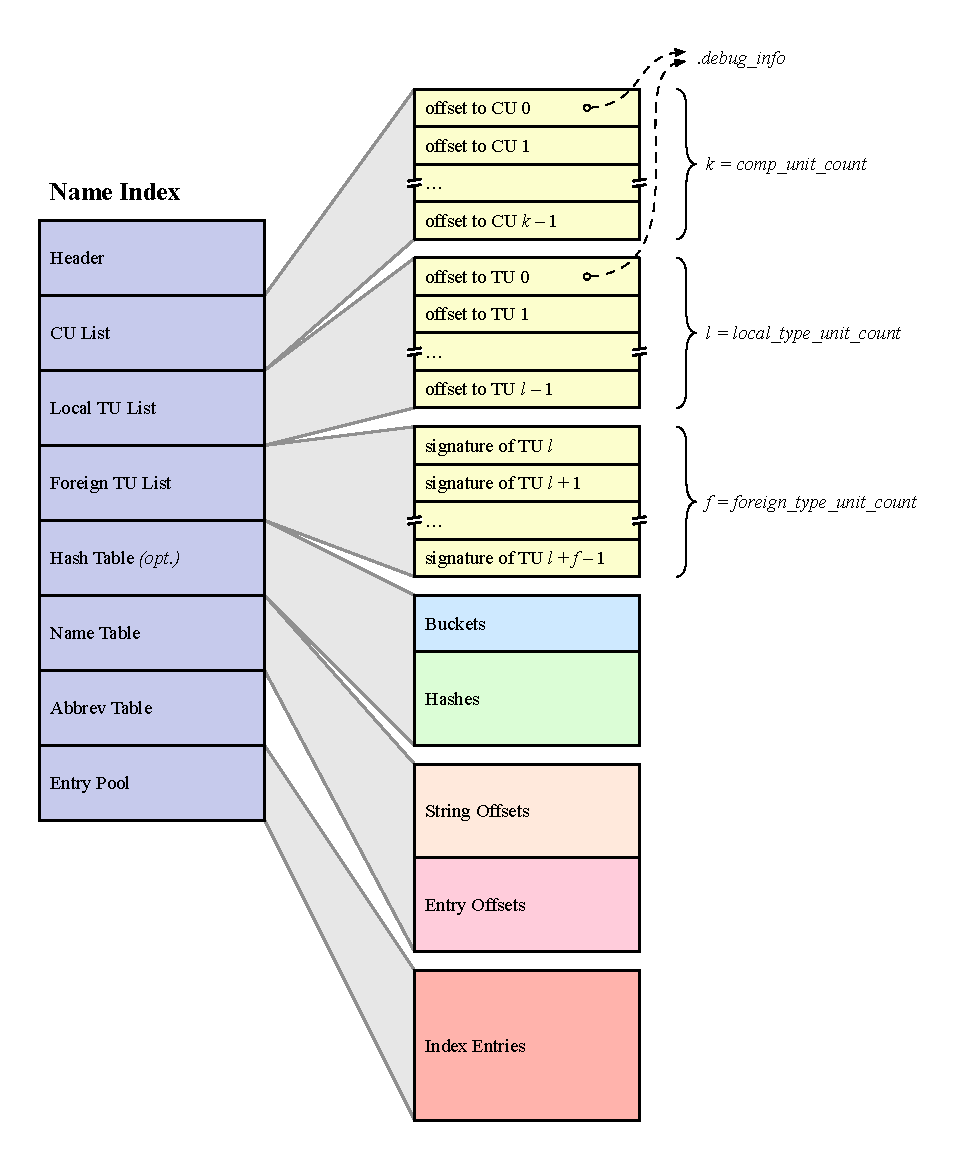
\includegraphics[keepaspectratio=true,scale=1.0]{name-index-drawings-6p1}

\begin{tikzpicture}[
  every node/.style={node font=\small, anchor=north west, text height=.8em, text depth=.2em, inner sep=4pt, outer ysep=0},
  caption/.style={node font=\small \bfseries, text width=90pt},
  overview/.style={draw, node font=\small, minimum height=28pt, text width=80pt},
  detail1/.style={draw, minimum height=14pt, text width=116pt},
  detail2/.style={draw, minimum height=28pt, text width=116pt},
  detail3/.style={draw, minimum height=48pt, text width=116pt},
  detail4/.style={draw, minimum height=72pt, text width=116pt},
  ellip/.style={draw, shape=broken rectangle, minimum height=14pt, text width=116pt},
  explode/.style={draw=black!50, fill=black!20, line join=bevel},
  header/.style={fill=headerblue},
  culist/.style={fill=cutuyellow},
  buckets/.style={fill=bucketsblue},
  hashes/.style={fill=hashesgreen},
  stroffsets/.style={fill=stroffsetspink},
  entryoffsets/.style={fill=entryoffsetspink},
  indexentries/.style={fill=indexentriesorange}
]

% Name Table Overview

\begin{scope}[start chain=going below, node distance=0]
  \node           [on chain,caption]  {Name Index};
  \node (header)  [on chain,overview,header] {Header};
  \node (culist)  [on chain,overview,header] {CU List};
  \node (ltulist) [on chain,overview,header] {Local TU List};
  \node (ftulist) [on chain,overview,header] {Foreign TU List};
  \node (hash)    [on chain,overview,header] {Hash Table};
  \node (names)   [on chain,overview,header] {Name Table};
  \node (abbrev)  [on chain,overview,header] {Abbrev Table};
  \node (pool)    [on chain,overview,header] {Entry Pool};
\end{scope}

% Exploded View of CU List

\begin{scope}[start chain=going below, node distance=0, shift={($(header.north east) + (72pt,18pt)$)}]
  \node (cu0) [on chain,detail1,culist] {offset to CU 0};
  \node (cu1) [on chain,detail1,culist] {offset to CU 1};
  \node (cu2) [on chain,ellip,culist]   {\dots};
  \node (cu3) [on chain,detail1,culist] {offset to CU $k - 1$};
\end{scope}

\begin{scope}[on background layer]
  \filldraw [explode] (culist.north east) -- (cu0.north west) -- (cu3.south west) -- (culist.south east) -- cycle;
\end{scope}

\path [decoration={brace,amplitude=6pt}] ([xshift=9pt]cu0.north east)
      [draw,decorate] -- ([xshift=9pt]cu3.south east)
      node [midway,right,inner xsep=9pt] {\texttt{comp\_unit\_count} $(= k)$};

% Exploded View of Local TU List

\begin{scope}[start chain=going below, node distance=0, shift={($(cu3.south west) + (0,-9pt)$)}]
  \node (ltu0) [on chain,detail1,culist] {offset to TU 0};
  \node (ltu1) [on chain,detail1,culist] {offset to TU 1};
  \node (ltu2) [on chain,ellip,culist]   {\dots};
  \node (ltu3) [on chain,detail1,culist] {offset to TU $t - 1$};
\end{scope}

\begin{scope}[on background layer]
  \filldraw [explode] (ltulist.north east) -- (ltu0.north west) -- (ltu3.south west) -- (ltulist.south east) -- cycle;
\end{scope}

\path [decoration={brace,amplitude=6pt}] ([xshift=9pt]ltu0.north east)
      [draw,decorate] -- ([xshift=9pt]ltu3.south east)
      node [midway,right,inner xsep=9pt] {\texttt{local\_type\_unit\_count} $(= t)$};

% Exploded View of Foreign TU List

\begin{scope}[start chain=going below, node distance=0, shift={($(ltu3.south west) + (0,-9pt)$)}]
  \node (ftu0) [on chain,detail1,culist] {signature of TU $t$};
  \node (ftu1) [on chain,detail1,culist] {signature of TU $t + 1$};
  \node (ftu2) [on chain,ellip,culist]   {\dots};
  \node (ftu3) [on chain,detail1,culist] {signature of TU $t + f - 1$};
\end{scope}

\begin{scope}[on background layer]
  \filldraw [explode] (ftulist.north east) -- (ftu0.north west) -- (ftu3.south west) -- (ftulist.south east) -- cycle;
\end{scope}

\path [decoration={brace,amplitude=6pt}] ([xshift=9pt]ftu0.north east)
      [draw,decorate] -- ([xshift=9pt]ftu3.south east)
      node [midway,right,inner xsep=9pt] {\texttt{foreign\_type\_unit\_count} $(= f)$};

% Exploded View of Hash Table

\begin{scope}[start chain=going below, node distance=0, shift={($(ftu3.south west) + (0,-9pt)$)}]
  \node (hash0) [on chain,detail2,buckets] {Buckets};
  \node (hash1) [on chain,detail3,hashes]  {Hashes};
\end{scope}

\begin{scope}[on background layer]
  \filldraw [explode] (hash.north east) -- (hash0.north west) -- (hash1.south west) -- (hash.south east) -- cycle;
\end{scope}

% Exploded View of Name Table

\begin{scope}[start chain=going below, node distance=0, shift={($(hash1.south west) + (0,-9pt)$)}]
  \node (name0) [on chain,detail3,stroffsets]   {String Offsets};
  \node (name1) [on chain,detail3,entryoffsets] {Entry Offsets};
\end{scope}

\begin{scope}[on background layer]
  \filldraw [explode] (names.north east) -- (name0.north west) -- (name1.south west) -- (names.south east) -- cycle;
\end{scope}

% Exploded View of Entry Pool

\begin{scope}[shift={($(name1.south west) + (0,-9pt)$)}]
  \node (pool0) [detail4,indexentries] {Index Entries};
\end{scope}

\begin{scope}[on background layer]
  \filldraw [explode] (pool.north east) -- (pool0.north west) -- (pool0.south west) -- (pool.south east) -- cycle;
\end{scope}

%
\path [decoration={brace,amplitude=6pt}] ([xshift=9pt]hash0.north east)
      [draw,decorate] -- ([xshift=9pt]pool0.south east)
      node [midway,right,inner xsep=9pt] {\textit{see figure part 2 on next page}};

% Arrows pointing to .debug_info

\begin{scope}[shift={($(cu0.north east) + (15pt,27pt)$)}]
  \node (debuginfo) {\textit{.debug\_info}};
\end{scope}

\path ([xshift=28pt]cu0.center) coordinate (p1);
\path ([xshift=14pt]p1) coordinate (c1);
\path ([yshift=2pt]debuginfo.west) coordinate (p2);
\path ([xshift=-14pt]p2) coordinate (c2);
\draw [dashed,{Circle[open]}-{Stealth[]}] (p1) .. controls (c1) and (c2) .. (p2);

\path ([xshift=28pt]ltu0.center) coordinate (p3);
\path ([xshift=60pt]p3) coordinate (c3);
\path ([yshift=-2pt]debuginfo.west) coordinate (p4);
\path ([shift={(-21pt,-7pt)}]p4) coordinate (c4);
\draw [dashed,{Circle[open]}-{Stealth[]}] (p3) .. controls (c3) and (c4) .. (p4);

\end{tikzpicture}

\caption{Name Index Layout}
\label{fig:nameindexlayoutpart1}
\end{center}
\end{figure}

\begin{figure}[p]
\figurepart{2}{2}
\begin{center}
%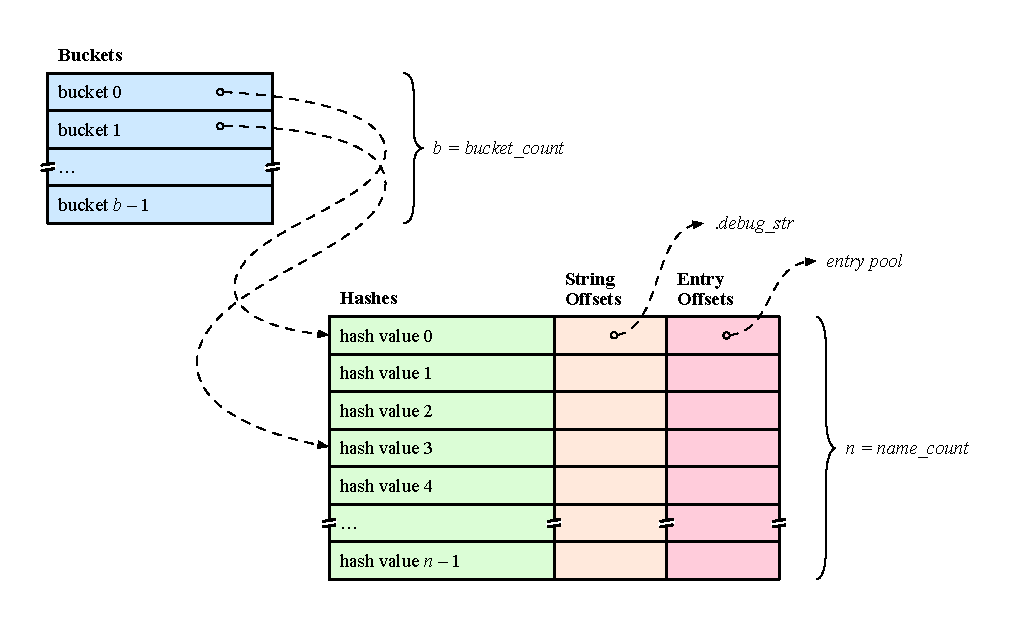
\includegraphics[keepaspectratio=true,scale=1.0]{name-index-drawings-6p2}

\begin{tikzpicture}[
  every node/.style={node font=\small, anchor=north west, text height=.8em, text depth=.2em, inner sep=4pt, outer ysep=0},
  % This diagram has a couple of two-line captions, so set the text depth
  % to make room for the second line.
  caption1/.style={node font=\small \bfseries, text depth=1.2em, text width=90pt},
  caption2/.style={node font=\small \bfseries, text depth=1.2em, text width=41pt},
  detail1/.style={draw, minimum height=14pt, text width=90pt},
  detail2/.style={draw, minimum height=14pt, text width=41pt},
  ellip1/.style={draw, shape=broken rectangle, minimum height=14pt, text width=90pt},
  ellip2/.style={draw, shape=broken rectangle, minimum height=14pt, text width=41pt},
  buckets/.style={fill=bucketsblue},
  hashes/.style={fill=hashesgreen},
  stroffsets/.style={fill=stroffsetspink},
  entryoffsets/.style={fill=entryoffsetspink}
]

% Buckets

\begin{scope}[start chain=going below, node distance=0]
  \node           [on chain,caption1]        {\\ Buckets};
  \node (bucket0) [on chain,detail1,buckets] {bucket 0};
  \node (bucket1) [on chain,detail1,buckets] {bucket 1};
  \node (bucket2) [on chain,ellip1,buckets]  {\dots};
  \node (bucket3) [on chain,detail1,buckets] {bucket $b - 1$};
\end{scope}

\path [decoration={brace,amplitude=6pt}] ([xshift=40pt]bucket0.north east)
      [draw,decorate] -- ([xshift=40pt]bucket3.south east)
      node [midway,right,inner xsep=9pt] {\texttt{bucket\_count} $(= b)$};

% Hashes

\begin{scope}[start chain=going below, node distance=0, shift={($(bucket3.south east) + (18pt,-24pt)$)}]
  \node (hashes) [on chain,caption1]       {\\ Hashes};
  \node (hash0)  [on chain,detail1,hashes] {hash value 1};
  \node (hash1)  [on chain,detail1,hashes] {hash value 2};
  \node (hash2)  [on chain,detail1,hashes] {hash value 3};
  \node (hash3)  [on chain,detail1,hashes] {hash value 4};
  \node (hash4)  [on chain,detail1,hashes] {hash value 5};
  \node (hash5)  [on chain,ellip1,hashes]  {\dots};
  \node (hash6)  [on chain,detail1,hashes] {hash value $n$};
\end{scope}

% String Offsets

\begin{scope}[start chain=going below, node distance=0, shift={($(hashes.north east)$)}]
  \node (strs) [on chain,caption2]           {String \\ Offsets};
  \node (str0) [on chain,detail2,stroffsets] {};
  \node (str1) [on chain,detail2,stroffsets] {};
  \node (str2) [on chain,detail2,stroffsets] {};
  \node (str3) [on chain,detail2,stroffsets] {};
  \node (str4) [on chain,detail2,stroffsets] {};
  \node (str5) [on chain,ellip2,stroffsets]  {};
  \node (str6) [on chain,detail2,stroffsets] {};
\end{scope}

% Entry Offsets

\begin{scope}[start chain=going below, node distance=0, shift={($(strs.north east)$)}]
  \node (entries) [on chain,caption2]             {Entry \\ Offsets};
  \node (entry0)  [on chain,detail2,entryoffsets] {};
  \node (entry1)  [on chain,detail2,entryoffsets] {};
  \node (entry2)  [on chain,detail2,entryoffsets] {};
  \node (entry3)  [on chain,detail2,entryoffsets] {};
  \node (entry4)  [on chain,detail2,entryoffsets] {};
  \node (entry5)  [on chain,ellip2,entryoffsets]  {};
  \node (entry6)  [on chain,detail2,entryoffsets] {};
\end{scope}

\path [decoration={brace,amplitude=6pt}] ([xshift=9pt]entry0.north east)
      [draw,decorate] -- ([xshift=9pt]entry6.south east)
      node [midway,right,inner xsep=9pt] {\begin{tabular}{c} 
                                          \texttt{name\_count} \\ 
                                                     $(= n)$ 
                                          \end{tabular}};

% Arrows pointing to .debug_str and entry pool

\path (str0.center) coordinate (p1);
\path ([xshift=18pt]p1) coordinate (c1);
\path ([shift={(36pt,45pt)}]p1) coordinate (p2);
\path ([xshift=-18pt]p2) coordinate (c2);
\draw [dashed,{Circle[open]}-{Stealth[]}] (p1) .. controls (c1) and (c2) .. (p2) node [anchor=west] {$.debug\_str$};

\path (entry0.center) coordinate (p3);
\path ([xshift=18pt]p3) coordinate (c3);
\path ([shift={(36pt,27pt)}]p3) coordinate (p4);
\path ([xshift=-18pt]p4) coordinate (c4);
\draw [dashed,{Circle[open]}-{Stealth[]}] (p3) .. controls (c3) and (c4) .. (p4) node [anchor=west] {$entry\ pool$};

% Arrows from buckets to hashes

\path ([xshift=24pt]bucket0.center) coordinate (p5);
\path ([xshift=130pt]p5) coordinate (c5);
\path ([xshift=-70pt]hash0.west) coordinate (c6);
\draw [dashed,{Circle[open]}-{Stealth[]}] (p5) .. controls (c5) and (c6) .. (hash0.west);

\path ([xshift=24pt]bucket1.center) coordinate (p7);
\path ([xshift=120pt]p7) coordinate (c7);
\path ([xshift=-144pt]hash3.west) coordinate (c8);
\draw [dashed,{Circle[open]}-{Stealth[]}] (p7) .. controls (c7) and (c8) .. (hash3.west);

\end{tikzpicture}

\vspace{15mm}

%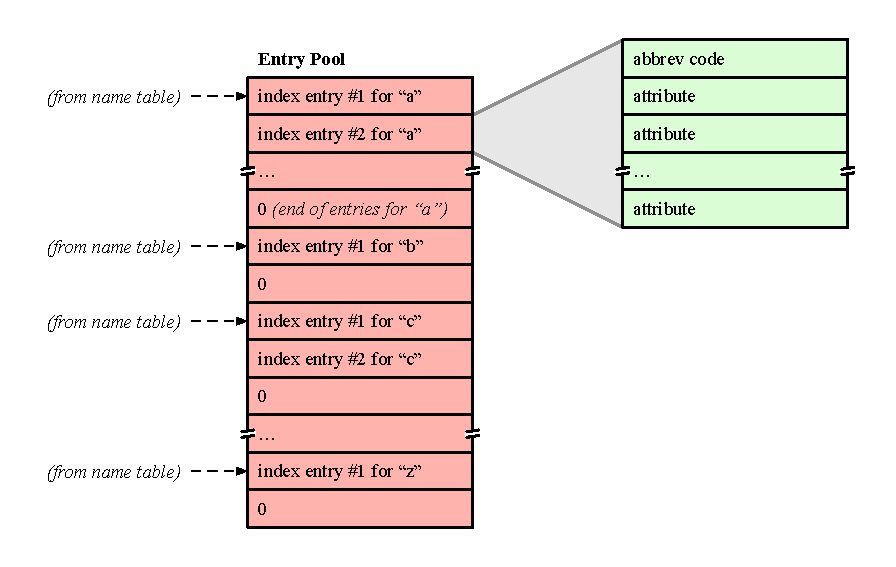
\includegraphics[keepaspectratio=true,scale=1.0]{name-index-drawings-6p3}
\begin{tikzpicture}[
  every node/.style={node font=\small, anchor=north west, text height=.8em, text depth=.2em, inner sep=4pt, outer ysep=0},
  caption/.style={node font=\small \bfseries, text width=120pt},
  detail/.style={draw, node font=\small, minimum height=14pt, text width=120pt},
  ellip/.style={draw, shape=broken rectangle, minimum height=14pt, text width=120pt},
  explode/.style={draw=black!50, fill=black!20, line join=bevel},
  indexentries/.style={fill=indexentriesorange}
]

% Entry Pool

\begin{scope}[start chain=going below, node distance=0]
  \node           [on chain,caption]             {Entry Pool};
  \node (entry0)  [on chain,detail,indexentries] {index entry \#1 for ``a''};
  \node (entry1)  [on chain,detail,indexentries] {index entry \#2 for ``a''};
  \node (entry2)  [on chain,ellip,indexentries]  {\dots};
  \node (entry3)  [on chain,detail,indexentries] {0 \textit{(end of entries for ``a'')}};
  \node (entry4)  [on chain,detail,indexentries] {index entry \#1 for ``b''};
  \node (entry5)  [on chain,detail,indexentries] {index entry \#2 for ``b''};
  \node (entry6)  [on chain,ellip,indexentries]  {\dots};
  \node (entry7)  [on chain,detail,indexentries] {0};
  \node (entry8)  [on chain,detail,indexentries] {index entry \#1 for ``c''};
  \node (entry9)  [on chain,ellip,indexentries]  {\dots};
\end{scope}

% Exploded Index Entry

\begin{scope}[start chain=going below, node distance=0, shift={($(entry1.north east) + (60pt,30pt)$)}]
  \node (abbrev) [on chain,detail,indexentries] {abbrev code};
  \node (attr1)  [on chain,detail,indexentries] {attribute};
  \node (attr2)  [on chain,detail,indexentries] {attribute};
  \node (attr3)  [on chain,ellip,indexentries]  {\dots};
  \node (attr4)  [on chain,detail,indexentries] {attribute};
\end{scope}

\begin{scope}[on background layer]
  \filldraw [explode] (entry1.north east) -- (abbrev.north west) -- (attr4.south west) -- (entry1.south east) -- cycle;
\end{scope}

% Arrows

\node (from1) [anchor=east] at ([xshift=-36pt]entry0.west) {\textit{(from name table)}};
\draw [dashed,-{Stealth[]}] (from1) -- (entry0.west);

\node (from2) [anchor=east] at ([xshift=-36pt]entry4.west) {\textit{(from name table)}};
\draw [dashed,-{Stealth[]}] (from2) -- (entry4.west);

\node (from2) [anchor=east] at ([xshift=-36pt]entry7.west) {\textit{(from name table)}};
\draw [dashed,-{Stealth[]}] (from2) -- (entry7.west);

\end{tikzpicture}

\vspace{3mm}
%\caption{Name Index Layout \textit{(concluded)}}
Figure~\ref{fig:nameindexlayoutpart1}: Name Index Layout \textit{(concluded)}
%\label{fig:nameindexlayoutpart2}
\end{center}
\end{figure}

The formats of the header and the hash lookup table are described
in Section \refersec{chap:datarepresentationofthenameindex}.

The list of CUs and the list of local TUs are each an array of
offsets, each of which is the offset of a compile unit or a type unit
in the \dotdebuginfo{} section. For a per-CU index, there is a single CU
entry, and there may be a TU entry for each type unit generated in the
same translation unit as the single CU. For a per-module index, there
will be one CU entry for each compile unit in the module, and one TU
entry for each unique type unit in the module. Each list is indexed
starting at 0.

The list of foreign TUs is an array of 64-bit (\DWFORMrefsigeight) type
signatures, representing types referenced by the index whose
definitions have been placed in a different object file (that is, a split
DWARF object). This list may be empty. 
The foreign TU list immediately follows the local TU list 
and they both use the same index, so that if there are $N$ local TU entries, 
the index for the first foreign TU is $N$.

The name table is logically a table with a row for each unique name in
the index, and two columns. The first column contains a reference to
the name, as a string. The second column contains the offset within
the entry pool of the list of index entries for the name.

\needlines{4}
The abbreviations table describes the formats of the entries in the
entry pool. Like the DWARF abbreviations table in the \dotdebugabbrev{}
section, it defines one or more abbreviation codes. Each abbreviation
code provides a DWARF tag value followed by a list of pairs that
defines an attribute and form code used by entries with that
abbreviation code.

The entry pool contains all the index entries, grouped by name. The
second column of the name list points to the first index entry for the
name, and all the index entries for that name are placed one after the
other.

Each index entry begins with an unsigned LEB128 abbreviation code.
The  abbreviation list for that code provides the DWARF tag value for
the entry as well as the set of attributes provided by the entry and
their forms.

\needlines{4}
The standard attributes are:
\begin{itemize}
\item Compilation Unit (CU), a reference to an entry in the list of
    CUs. In a per-CU index, index entries without this attribute
    implicitly refer to the single CU.

\item Type Unit (TU), a reference to an entry in the list of local
    or foreign TUs.

\item Debugging information entry offset within the CU or TU.

\item Parent debugging information entry, 
    a reference to the index entry for the parent.
    This is represented as the offset of the entry relative to
    the start of the entry pool.

\item Type hash, an 8-byte hash of the type declaration.

\end{itemize}

\needlines{6}
It is possible that an indexed debugging information entry
has a parent that is not
indexed (for example, if its parent does not have a name attribute). 
In such a case, a parent attribute may point to a nameless index
entry (that is, one that cannot be reached from any entry in the
name table), or it may point to the nearest ancestor that does
have an index entry.

A producer may define additional vendor-specific attributes, 
and a consumer will be able to ignore and skip over any attributes 
it is not prepared to handle.

\needlines{4}
When an index entry refers to a foreign type unit, it may have
attributes for both CU and (foreign) TU. For such entries, the CU
attribute gives the consumer a reference to the CU that may be used to
locate a \splitDWARFobjectfile{} that contains the type unit.

\textit{The type hash attribute, not to be confused with the type signature
for a TU, may be provided for type entries whose declarations are not
in a type unit, for the convenience of link-time or post-link
utilities that wish to de-duplicate type declarations across
compilation units. The type hash, however, is computed by the
same method as specified for type signatures.}

The last entry for each name is followed by a zero byte that
terminates the list. There may be gaps between the lists.

\subsubsection{Per-CU versus Per-Module Indexes}
\label{chap:percuvspermoduleindexes}
\textit{In a per-CU index, the CU list may have only a single entry, 
and index entries may omit the CU attribute. (Cross-module or link-time
optimization, however, may produce an object file with several compile
units in one object. A compiler in this case may produce a separate
index for each CU, or a combined index for all CUs. In the latter
case, index entries will require the CU attribute.) Most name table
entries may have only a single index entry for each, but sometimes a
name may be used in more than one context and will require multiple
index entries, each pointing to a different debugging information
entry.}

\textit{When linking object files containing per-CU indexes, the 
linker may choose to concatenate the indexes as ordinary sections, 
or it may choose to combine the input indexes into a single 
per-module index.}

\textit{A per-module index will contain a number of CUs, and each index 
entry contains a CU attribute or a TU attribute to identify which 
CU or TU contains the debugging information entry being indexed. When a
given name is used in multiple CUs or TUs, it will typically have a
series of index entries pointing to each CU or TU where it is declared. 
For example, an index entry for a \addtoindex{C++} namespace needs to
list each occurrence, since each CU may contribute additional names to
the namespace, and the consumer needs to find them all. On the
other hand, some index entries do not need to list more than one
definition; for example, with the one-definition rule in \addtoindex{C++},
duplicate entries for a function may be omitted, since the consumer
only needs to find one declaration. Likewise, a per-module index needs
to list only a single copy of a type declaration contained in a type
unit.}

\textit{For the benefit of link-time or post-link utilities that consume
per-CU indexes and produce a per-module index, the per-CU index
entries provide the tag encoding for the original debugging
information entry, and may provide a type hash for certain types that
may benefit from de-duplication. For example, the standard declaration
of the typedef \texttt{uint32\_t} is likely to occur in many CUs, but a
combined per-module index needs to retain only one; a user declaration
of a typedef \texttt{mytype} may refer to a different type at each
occurrence, and a combined per-module index retains each unique
declaration of that type.}


\subsubsection{Data Representation of the Name Index}
\label{chap:datarepresentationofthenameindex}
The name index is placed in a section named \dotdebugnames, and
consists of the eight parts described in the following sections.

\subsubsubsection{Section Header}
\label{chap:sectionheader}
The section header contains the following fields:
\begin{enumerate}[1. ]
\item \texttt{unit\_length} (\livelink{datarep:initiallengthvalues}{initial length}) \\
\addttindexx{unit\_length}
The length of this contribution to the name index section,
not including the length field itself.

\item \texttt{version} (\HFTuhalf) \\
A version number\addtoindexx{version number!name index table} 
(see Section \refersec{datarep:nameindextable}). 
This number is specific to the name index table and is
independent of the DWARF version number.

\item \textit{padding} (\HFTuhalf) \\
Reserved to DWARF (must be zero). 

\item \texttt{comp\_unit\_count} (\HFTuword) \\
The number of CUs in the CU list.

\item \texttt{local\_type\_unit\_count} (\HFTuword) \\
The number of TUs in the local TU list.

\item \texttt{foreign\_type\_unit\_count} (\HFTuword) \\
The number of TUs in the foreign TU list.

\item \texttt{bucket\_count} (\HFTuword) \\
The number of hash buckets in the hash lookup table. 
If there is no hash lookup table, this field contains 0.

\item \texttt{name\_count} (\HFTuword) \\
The number of unique names in the index.

\item \texttt{abbrev\_table\_size} (\HFTuword) \\
The size in bytes of the abbreviations table.

\item \texttt{augmentation\_string\_size} (\HFTuword) \\
The size in bytes of the augmentation string. This value is
rounded up to a multiple of 4.

\item \texttt{augmentation\_string} (\HFTaugstring) \\
A vendor-specific augmentation string, which provides additional 
information about the contents of this index. If provided, the string
begins with a 4-character vendor ID. The remainder of the
string is meant to be read by a cooperating consumer, and its
contents and interpretation are not specified here. The
string is padded with null characters to a multiple of
four bytes in length.

\textit{The presence of an unrecognised augmentation string may make it impossible
for a consumer to process data in the \dotdebugnames{} section.}

\end{enumerate}

\needlines{4}
\subsubsubsection{List of CUs}
The list of CUs immediately follows the header. Each entry in the 
list is an offset of the corresponding compilation unit
in the \dotdebuginfo{} section.
In the DWARF-32 format, a section offset is 4 bytes, 
while in the DWARF-64 format, a section offset is 8 bytes.

The total number of entries in the list is given by \texttt{comp\_unit\_count}.
There must be at least one CU.

\needlines{4}
\subsubsubsection{List of Local TUs}
The list of local TUs immediately follows the list of CUs. Each 
entry in the list is an offset of the corresponding type unit
in the \dotdebuginfo{} section. 
In the DWARF-32 format, a section offset is 4 bytes, 
while in the DWARF-64 format, a section offset is 8 bytes.

The total number of entries in the list is given by
\texttt{local\_type\_unit\_count}. This list may be empty.

\subsubsubsection{List of Foreign TUs}
The list of foreign TUs immediately follows the list of local TUs.
Each entry in the list is a 8-byte type signature (as described by
\DWFORMrefsigeight).

The number of entries in the list is given by \texttt{foreign\_type\_unit\_count}.
This list may be empty.

\needlines{4}
\subsubsubsection{Hash Lookup Table}
The optional hash lookup table immediately follows the list of type signatures.

The hash lookup table is actually two separate arrays: an array of
buckets, followed immediately by an array of hashes. The number of
entries in the buckets array is given by \texttt{bucket\_count}, and the number
of entries in the hashes array is given by \texttt{name\_count}. Each array
contains 4-byte unsigned integers.

\needlines{4}
Symbols are entered into the hash table by first computing a hash
value from the symbol name. The hash is computed 
using the "DJB" hash function\addtoindexx{DJB hash function} 
described in Section \refersec{datarep:nametablehashfunction}.
Given a hash value for the symbol,
the symbol is entered into a bucket whose index is the hash value
modulo \texttt{bucket\_count}. The buckets array is indexed starting at 0.

\bb
For the purposes of the hash computation, each symbol name should be
folded according to the simple case folding algorithm defined in the
"Caseless Matching" subsection of Section 5.18 ("Case Mappings") of
the \addtoindex{Unicode} Standard, Version 9.0.0. The original symbol 
name, as it appears in the source code, should be stored in the name 
table.

\textit{Thus, two symbols that differ only by case will hash to
the same slot, but the consumer will be able to distinguish the names
when appropriate.}

\textit{The simple case folding algorithm is further described
in the CaseFolding.txt file distributed with the \addtoindex{Unicode} 
Character Database. That file defines four classes of mappings: 
Common (C), Simple (S), Full (F), and Turkish (T). 
The hash computation specified here uses the C + S mappings only, 
which do not affect the total length of the string.}
\eb

Each bucket contains the index of an entry in the hashes array. The
hashes array is indexed starting at 1, and an empty bucket is
represented by the value 0.

\needlines{4}
The hashes array contains a sequence of the full hash values for each
symbol. All symbols that have the same index into the bucket list 
follow one another in the hashes array, and the indexed entry in 
the bucket list refers to the first symbol. 
When searching for a symbol, the search 
starts at the index given by the bucket, and continues either until a
matching symbol is found or until a hash value from a different bucket
is found. If two different symbol names produce the same hash value,
that hash value will occur twice in the hashes array. Thus, if a
matching hash value is found, but the name does not match, the search
continues visiting subsequent entries in the hashes table.

When a matching hash value is found in the hashes array, the index of
that entry in the hashes array is used to find the corresponding entry
in the name table.

\needlines{6}
\subsubsubsection{Name Table}
\label{chap:nametable}
The name table immediately follows the hash lookup table. It
consists of two arrays: an array of string offsets, followed
immediately by an array of entry offsets. The items in both
arrays are section offsets: 4-byte unsigned integers for the
DWARF-32 format or 8-byte unsigned integers for the DWARF-64
format. The string offsets in the first array refer to names in
the \dotdebugstr{} (or \dotdebugstrdwo) section. The entry offsets
in the second array refer to index entries, and are relative to
the start of the entry pool area.

These two arrays are indexed starting at 1, and correspond 
one-to-one with each other. The length of each array is
given by \texttt{name\_count}.

If there is a hash lookup table, the hashes array corresponds on
a one-to-one basis with the string offsets array and with the
entry offsets array.

\textit{If there is no hash lookup table, there is no ordering
requirement for the name table.}

\needlines{6}
\subsubsubsection{Abbreviations Table}
The abbreviations table immediately follows the name table. This table
consists of a series of abbreviation declarations. Its size is given
by \texttt{abbrev\_table\_size}.

Each abbreviation declaration defines the tag and other attributes for
a particular form of index entry. Each declaration starts with an
unsigned LEB128 number representing the abbreviation code itself. It
is this code that appears at the beginning of an index entry. The
abbreviation code must not be 0.

The abbreviation code is followed by another unsigned LEB128 number
that encodes the tag of the debugging information entry corresponding
to the index entry.

Following the tag encoding is a series of attribute specifications.
Each attribute consists of two parts: an unsigned LEB128 number that
represents the index attribute, and another unsigned LEB128 number
that represents the attribute's form (as described in 
Section \refersec{datarep:attributeencodings}). The series of attribute 
specifications ends with an entry containing 0 for the attribute and 
0 for the form.

The index attributes and their meanings are listed in 
Table \referfol{tab:indexattributeencodings}.

\begin{centering}
\setlength{\extrarowheight}{0.1cm}
\begin{longtable}{l|l}
  \caption{Index attribute encodings} \label{tab:indexattributeencodings}\\
  \hline \bfseries Attribute name &\bfseries Meaning \\ \hline
\endfirsthead
  \bfseries Attribute name &\bfseries Meaning \\ \hline
\endhead
  \hline \emph{Continued on next page}
\endfoot
  \hline
\endlastfoot
\DWIDXcompileunitTARG & Index of CU                                  \\
\DWIDXtypeunitTARG    & Index of TU (\mbox{local} or foreign)        \\
\DWIDXdieoffsetTARG   & Offset of DIE within CU or TU                \\
\DWIDXparentTARG      & Index of name \mbox{table} entry for parent  \\
\DWIDXtypehashTARG    & Hash of type \mbox{declaration}              \\
\end{longtable}
\end{centering}

The abbreviations table ends with an entry consisting of a single 0
byte for the abbreviation code. The size of the table given by
\texttt{abbrev\_table\_size} may include optional padding following the
terminating 0 byte.

\subsubsubsection{Entry Pool}
The entry pool immediately follows the abbreviations table. 
Each entry in the entry offsets array in the name table (see 
Section \ref{chap:nametable})
points to an offset in the entry pool, where a series
of index entries for that name is located.

\needlines{4}
Each index entry in the series begins with an abbreviation code, and is
followed by the attributes described by the abbreviation declaration
for that code. The last index entry in the series is followed by a
terminating entry whose abbreviation code is 0.

Gaps are not allowed between entries in a series (that is, the entries
for a single name must all be contiguous), but there may be gaps
between series.

\textit{For example, a producer/consumer combination may find
it useful to maintain alignment.}

The size of the entry pool is the remaining size of the contribution to
the index section, as defined by the \texttt{unit\_length} header field.

\subsection{Lookup by Address}
\label{chap:lookupbyaddress}
For \addtoindexx{lookup!by address}
lookup by address, a table is maintained in a separate
\addtoindexx{accelerated access!by address}
object file section called 
\dotdebugaranges{}. The table consists
of sets of variable length entries, each set describing the
portion of the program\textquoteright{}s address space that is covered by
a single compilation unit.

\needlines{4}
Each set begins with a header containing five values:
\begin{enumerate}[1. ]
\item \texttt{unit\_length} (\livelink{datarep:initiallengthvalues}{initial length}) \\
\addttindexx{unit\_length}
The length of this contribution to the address lookup section,
not including the length field itself.

\item \texttt{version} (\HFTuhalf) \\
A version number\addtoindexx{version number!address lookup table}
(see Section \refersec{datarep:addrssrangetable}). 
This number is specific to the address lookup table and is
independent of the DWARF version number.

\item \texttt{debug\_info\_offset} (section offset) \\
The offset from the
\addtoindexx{section offset!in .debug\_aranges header}
beginning of the \dotdebuginfo{} section of the
compilation unit header referenced by the set.

\item \texttt{address\_size} (\HFTubyte) \\
The \addtoindex{size of an address}
in bytes on
\addttindexx{address\_size}
the target architecture. For 
\addtoindexx{address space!segmented}
segmented addressing, this is
the size of the offset portion of the address.

\item \HFNsegmentselectorsize{} (\HFTubyte) \\
The size of a segment selector in
bytes on the target architecture. If the target system uses
a flat address space, this value is 0.

\end{enumerate}

This header is followed by a variable number of address range
descriptors. Each descriptor is a triple consisting of a
segment selector, the beginning address within that segment
of a range of text or data covered by some entry owned by
the corresponding compilation unit, followed by the non-zero
length of that range. A particular set is terminated by an
entry consisting of three zeroes. 
When the \HFNsegmentselectorsize{} value
is zero in the header, the segment selector is omitted so that
each descriptor is just a pair, including the terminating
entry. By scanning the table, a debugger can quickly decide
which compilation unit to look in to find the debugging
information for an object that has a given address.

\textit{If the range of addresses covered by the text and/or data
of a compilation unit is not contiguous, then there may be
multiple address range descriptors for that compilation unit.}


\section{Line Number Information}
\label{chap:linenumberinformation}
\textit{A source\dash level debugger needs to know how to
\addtoindexx{line number information|see{\textit{also} statement list attribute}}
associate locations in the source files with the corresponding
machine instruction addresses in the executable or the shared 
object files used by that executable object file. Such an
association makes it possible for the debugger user
to specify machine instruction addresses in terms of source
locations. This is done by specifying the line number
and the source file containing the statement. The debugger
can also use this information to display locations in terms
of the source files and to single step from line to line,
or statement to statement.}

Line number information generated for a compilation unit is
represented in the 
\dotdebugline{} section of an object file, and optionally
also in the \dotdebuglinestr{} section, and
is referenced by a corresponding compilation unit debugging
information entry 
(see Section \refersec{chap:fullandpartialcompilationunitentries}) 
in the \dotdebuginfo{} section.

\textit{Some computer architectures employ more than one instruction
set (for example, the ARM 
\addtoindexx{ARM instruction set architecture}
and 
MIPS architectures support
\addtoindexx{MIPS instruction set architecture}
a 32-bit as well as a 16-bit instruction set). Because the
instruction set is a function of the program counter, it is
convenient to encode the applicable instruction set in the
\dotdebugline{} section as well.}

\textit{If space were not a consideration, the information provided
in the \dotdebugline{} 
section could be represented as a large
matrix, with one row for each instruction in the emitted
object code. The matrix would have columns for:}
\begin{itemize}
\item \textit{the source file name}
\item \textit{the source line number}
\item \textit{the source column number}
\item \textit{whether this instruction is the beginning of a source statement}
\item \textit{whether this instruction is the beginning of a \addtoindex{basic block}}
\item \textit{and so on}
\end{itemize}
\textit{Such a matrix, however, would be impractically large. We
shrink it with two techniques. First, we delete from
the matrix each row whose file, line, source column and
discriminator\addttindexx{discriminator} 
is identical with that of its
predecessors. Any deleted row would never be the beginning of
a source statement. Second, we design a byte-coded language
for a state machine and store a stream of bytes in the object
file instead of the matrix. This language can be much more
compact than the matrix. To the line number information a 
consumer must \doublequote{run} the state machine
to generate the matrix for each compilation unit of interest.
The concept of an encoded matrix also leaves
room for expansion. In the future, columns can be added to the
matrix to encode other things that are related to individual
instruction addresses.}

\needlines{10}
\subsection{Definitions}
\label{chap:definitions}
The following terms are used in the description of the line
number information format:

\begin{longtable} {lP{9cm}}
state machine &
The hypothetical machine used by a consumer of the line number
information to expand the byte\dash coded 
instruction stream into a matrix of
line number information. \\

line number program &
A series of byte\dash coded 
line number information instructions representing
one compilation unit. \\

\addtoindex{basic block} &
 A sequence of instructions where only the first instruction may be a
branch target and only the last instruction may transfer control. A
subprogram invocation is defined to be an exit from a 
\addtoindex{basic block}.

\textit{A \addtoindex{basic block} does not 
necessarily correspond to a specific source code
construct.} \\

sequence &
A series of contiguous target machine instructions. One compilation unit
may emit multiple sequences (that is, not all instructions within a
compilation unit are assumed to be contiguous). \\
\end{longtable}

\needlines{8}
\subsection{State Machine Registers}
\label{chap:statemachineregisters}
The line number information state machine has a number of  
registers as shown in Table \referfol{tab:statemachineregisters}.

\begin{longtable}{l|P{9cm}}
  \caption{State machine registers } \label{tab:statemachineregisters} \\
  \hline \bfseries Register name&\bfseries Meaning\\ \hline
\endfirsthead
  \bfseries Register name&\bfseries Meaning\\ \hline
\endhead
  \hline \emph{Continued on next page}
\endfoot
  \hline
\endlastfoot
\addtoindexi{\texttt{address}}{address register!in line number machine}&
The program\dash counter value corresponding to a machine instruction
generated by the compiler. \\

\addttindex{op\_index} &
An unsigned integer representing the index of an operation within a VLIW
instruction. The index of the first operation is 0. For non-VLIW
architectures, this register will always be 0.  \\

\addttindex{file} &
An unsigned integer indicating the identity of the source file
corresponding to a machine instruction. \\

\addttindex{line} &
An unsigned integer indicating a source line number. Lines are numbered
beginning at 1. The compiler may emit the value 0 in cases where an
instruction cannot be attributed to any source line. \\

\addttindex{column} &
An unsigned integer indicating a column number within a source line.
Columns are numbered beginning at 1. The value 0 is reserved to indicate
that a statement begins at the \doublequote{left edge} of the line. \\

\addttindex{is\_stmt} &
A boolean indicating that the current instruction is a recommended
breakpoint location. A recommended breakpoint location 
is intended to \doublequote{represent} a line, a 
statement and/or a semantically distinct subpart of a
statement. \\

\addttindex{basic\_block}  &
A boolean indicating that the current instruction is the beginning of a
\addtoindex{basic block}. \\

\addttindex{end\_sequence} &
A boolean indicating that the current address is that of the first byte after
the end of a sequence of target machine instructions. 
\addttindex{end\_sequence}
terminates a sequence of lines; therefore other information in the same
row is not meaningful. \\

\addttindex{prologue\_end} &
A boolean indicating that the current address is one (of possibly many)
where execution should be suspended for a breakpoint at the entry of a
function. \\

\addttindex{epilogue\_begin} &
A boolean indicating that the current address is one (of possibly many)
where execution should be suspended for a breakpoint just prior to
the exit of a function. \\

\addttindex{isa} &
An unsigned integer whose value encodes the applicable
instruction set architecture for the current instruction.

\textit{The encoding of instruction sets should be shared by all
users of a given architecture. It is recommended that this
encoding be defined by the ABI authoring committee for each
architecture.} \\

\addttindex{discriminator} &
An unsigned integer identifying the block to which the
current instruction belongs. Discriminator values are assigned
arbitrarily by the DWARF producer and serve to distinguish
among multiple blocks that may all be associated with the
same source file, line, and column. Where only one block
exists for a given source position, the discriminator value
is be zero. \\
\end{longtable}

The \texttt{address} and \addttindex{op\_index} registers,
taken together, form an \addtoindex{operation pointer} that can 
reference any individual operation within the instruction stream.

At the beginning  of each sequence within a line number
program, the state of the registers is as show in Table
\refersec{tab:linenumberprograminitiastate}.
\begin{table}
\caption{Line number program initial state}
\label{tab:linenumberprograminitiastate}
\begin{center}
\begin{tabular}{l|p{9.5cm}}
\hline
\texttt{address} & 0 \\
\addttindex{op\_index} & 0 \\
\texttt{file} & 1 \\
\texttt{line} & 1 \\
\texttt{column} & 0 \\
\addttindex{is\_stmt} & determined by \addttindex{default\_is\_stmt} 
			in the line number program header \\
\addttindex{basic\_block}    & \doublequote{false} \addtoindexx{basic block} \\
\addttindex{end\_sequence}   & \doublequote{false} \\
\addttindex{prologue\_end}   & \doublequote{false} \\
\addttindex{epilogue\_begin} & \doublequote{false} \\
\addttindex{isa} & 0 \\
\addttindex{discriminator} & 0 \\
\hline
\end{tabular}
\end{center}
\vspace{5mm}
\end{table}

\textit{The 
\addttindex{isa} value 0 specifies that the instruction set is the
architecturally determined default instruction set. This may
be fixed by the ABI, or it may be specified by other means,
for example, by the object file description.}

\needlines{6}
\subsection{Line Number Program Instructions}
The state machine instructions in a line number program belong to one of three categories:

\begin{enumerate}[1. ]
\item special opcodes \\
These have a \HFTubyte{} opcode field and no operands.\vspace{1ex}

\textit{Most of the instructions in a 
line number program are special opcodes.}

\needlines{4}
\item standard opcodes \\
These have a \HFTubyte{} opcode field which may be followed by zero or more
\addtoindex{LEB128} operands (except for 
\mbox{\DWLNSfixedadvancepc,} see 
Section \refersec{chap:standardopcodes}).
The opcode implies the number of operands and their meanings, but the
line number program header also specifies the number of operands for
each standard opcode.

\needlines{4}
\item extended opcodes \\
These have a multiple byte format. The first byte is zero; the next bytes
are an unsigned LEB128\addtoindexx{LEB128!unsigned} integer giving the number of bytes in the
instruction itself (does not include the first zero byte or the size). The
remaining bytes are the instruction itself (which begins with a \HFTubyte{}
extended opcode). \\
\end{enumerate}


\subsection{The Line Number Program Header}
\label{chap:linenumberprogramheader}
The optimal encoding of line number information depends to a
certain degree upon the architecture of the target machine. The
line number program header provides information used by
consumers in decoding the line number program instructions for
a particular compilation unit and also provides information
used throughout the rest of the line number program.

The line number program for each compilation unit begins with
a header containing the following fields in order:

\begin{enumerate}[1. ]
\item \texttt{unit\_length} (\livelink{datarep:initiallengthvalues}{initial length})  \\
\addttindexx{unit\_length}
The size in bytes of the line number information for this
compilation unit, not including the length field itself
(see Section \refersec{datarep:initiallengthvalues}). 

\needlines{4}
\item \texttt{version} (\HFTuhalf) \\
A version number\addtoindexx{version number!line number information} 
(see Section \refersec{datarep:linenumberinformation}). 
This number is specific to
the line number information and is independent of the DWARF
version number. 

\item \texttt{address\_size} (\HFTubyte)\\
A 1-byte unsigned integer containing the size in bytes of an
address (or offset portion of an address for segmented addressing)
on the target system.
   
\textit{The \addttindex{address\_size} field is new in DWARF Version 5. 
It is needed to support the common practice of stripping all but 
the line number sections (\dotdebugline{} and \dotdebuglinestr{}) 
from an executable.}

\item \HFNsegmentselectorsize{} (\HFTubyte) \\
A 1-byte unsigned integer containing the size in bytes of a segment
selector on the target system.
   
\textit{The \HFNsegmentselectorsize{} field is new in DWARF Version 5. 
It is needed in combination with the \addttindex{address\_size} field 
to accurately characterize the address representation on the target 
system.}

\needlines{4}
\item \texttt{header\_length}  \\
The number of bytes following the \addttindex{header\_length} field to the
beginning of the first byte of the line number program itself.
In the \thirtytwobitdwarfformat, this is a 4-byte unsigned
length; in the \sixtyfourbitdwarfformat, this field is an
8-byte unsigned length 
(see Section \refersec{datarep:32bitand64bitdwarfformats}). 

\item \texttt{minimum\_instruction\_length} (\HFTubyte)  \\
\addttindexx{minimum\_instruction\_length}
The size in bytes of the smallest target machine
instruction. Line number program opcodes that alter
the \texttt{address} and \addttindex{op\_index}
registers use this and
\addttindex{maximum\_operations\_per\_instruction}
in their calculations. 

\needlines{9}
\item \texttt{maximum\_operations\_per\_instruction} (\HFTubyte) \\
The 
\addttindexx{maximum\_operations\_per\_instruction}
maximum number of individual operations that may be
encoded in an instruction. Line number program opcodes
that alter the \texttt{address} and 
\addttindex{op\_index} registers use this and
\addttindex{minimum\_instruction\_length} in their calculations.

For non-VLIW
architectures, this field is 1, the \addttindex{op\_index} register is always
0, and the \addtoindex{operation pointer} is simply the \texttt{address} register.

\needlines{4}
\item \texttt{default\_is\_stmt} (\HFTubyte) \\
\addttindexx{default\_is\_stmt}
The initial value of the \addttindex{is\_stmt} register.  

\textit{A simple approach
to building line number information when machine instructions
are emitted in an order corresponding to the source program
is to set \addttindex{default\_is\_stmt}
to \doublequote{true} and to not change the
value of the \addttindex{is\_stmt} register 
within the line number program.
One matrix entry is produced for each line that has code
generated for it. The effect is that every entry in the
matrix recommends the beginning of each represented line as
a breakpoint location. This is the traditional practice for
unoptimized code.}

\textit{A more sophisticated approach might involve multiple entries in
the matrix for a line number; in this case, at least one entry
(often but not necessarily only one) specifies a recommended
breakpoint location for the line number. \DWLNSnegatestmt{}
opcodes in the line number program control which matrix entries
constitute such a recommendation and 
\addttindex{default\_is\_stmt} might
be either \doublequote{true} or \doublequote{false.} This approach might be
used as part of support for debugging optimized code.}

\item \texttt{line\_base} (\HFTsbyte) \\
\addttindexx{line\_base}
This parameter affects the meaning of the special opcodes. See below.

\item \texttt{line\_range} (\HFTubyte) \\
\addttindexx{line\_range}
This parameter affects the meaning of the special opcodes. See below.

\needlines{4}
\item \texttt{opcode\_base} (\HFTubyte) \\
The 
\addttindexx{opcode\_base}
number assigned to the first special opcode.

\textit{Opcode base is typically one greater than the highest-numbered
\addttindexx{opcode\_base}
standard opcode defined for the specified version of the line
number information (12 in DWARF Versions 3, 4 and 5,
\addtoindexx{DWARF Version 3}
\addtoindexx{DWARF Version 4}
\addtoindexx{DWARF Version 5}
and 9 in
\addtoindexx{DWARF Version 2}
Version 2).  
If opcode\_base is less than the typical value,
\addttindexx{opcode\_base}
then standard opcode numbers greater than or equal to the
opcode base are not used in the line number table of this unit
(and the codes are treated as special opcodes). If \texttt{opcode\_base}
is greater than the typical value, then the numbers between
that of the highest standard opcode and the first special
opcode (not inclusive) are used for vendor specific extensions.}

\needlines{4}
\item \texttt{standard\_opcode\_lengths} (array of \HFTubyte) \\
\addttindexx{standard\_opcode\_lengths}
This array specifies the number of \addtoindex{LEB128} operands for each
of the standard opcodes. The first element of the array
corresponds to the opcode whose value is 1, and the last
element corresponds to the opcode whose value 
is \texttt{opcode\_base - 1}.

\textit{By increasing \texttt{opcode\_base}, and adding elements to this array,
\addttindexx{opcode\_base}
new standard opcodes can be added, while allowing consumers who
do not know about these new opcodes to be able to skip them.}

\textit{Codes for vendor specific extensions, if any, are described
just like standard opcodes.}

%%% Save the current enum counter so we can restart later
%%% End this enumeration so the following text is outdented to
%%% the left margin (because it applies to the many following
%%% items
\newcounter{saveenumi}
\setcounter{saveenumi}{\value{enumi}}
\end{enumerate}

\needlines{6}
\textit{The remaining fields provide information about the
source files used in the compilation. These fields
have been revised in \DWARFVersionV{} to support these
goals:}
\begin{itemize}
\item
    \textit{To allow new alternative means for a consumer to
    check that a file it can access is the same version
    as that used in the compilation.}
\item
    \textit{To allow a producer to collect file name strings
    in a new section (\dotdebuglinestr{}) that can be used
    to merge duplicate file name strings.}
\item
    \textit{To add the ability for producers to provide 
    vendor-defined information that can be skipped by a consumer
    that is unprepared to process it.}
\end{itemize}

\begin{enumerate}[1. ]
%%% Resume enumeration count where it left off above
\setcounter{enumi}{\value{saveenumi}}
\item \texttt{directory\_entry\_format\_count} (\HFTubyte) \\
\addttindexx{directory\_entry\_format\_count}
    A count of the number of entries that occur in the
    following \addttindex{directory\_entry\_format} field.

\needlines{8}
\item \texttt{directory\_entry\_format} (sequence of ULEB128 pairs) \\
\addttindexx{directory\_entry\_format}
    A sequence of directory entry format descriptions.
    Each description consists of a pair of ULEB128 values:
\begin{itemize}
\setlength{\itemsep}{0em}
\item A content type code (see 
Sections \refersec{chap:standardcontentdescriptions} and
\refersec{chap:vendordefinedcontentdescriptions}).

\item A form code using the attribute form codes
\end{itemize}

\needlines{4} 
\item \texttt{directories\_count} (ULEB128) \\
\addttindexx{directories\_count}
A count of the number of entries that occur in the
following directories field.

\needlines{4}    
\item \texttt{directories} (sequence of directory names) \\
\addttindexx{directories}
A sequence of directory names and optional related
information. Each entry is encoded as described
by the \addttindex{directory\_entry\_format} field.
   
Entries in this sequence describe each path that was
searched for included source files in this compilation,
including the compilation directory of the compilation.
(The paths include those directories specified by the
user for the compiler to search and those the compiler
searches without explicit direction.)
   
The first entry is the current directory of the compilation.
Each additional path entry is either a full path name or
is relative to the current directory of the compilation.
   
The line number program assigns a number (index) to each
of the directory entries in order, beginning with 0.
   
\textit{Prior to \DWARFVersionV, the current directory was not
represented in the directories field and a directory index
of 0 implicitly referred to that directory as found in the
\DWATcompdir{} attribute of the compilation unit 
debugging information entry. 
In \DWARFVersionV, the current directory is explicitly present
in the directories field. This is needed to support the
common practice of stripping all but the line number sections
(\dotdebugline{} and \dotdebuglinestr) from an executable.}

\textit{Note that if a \dotdebuglinestr{} section is present, 
both the compilation unit debugging information entry 
and the line number header can
share a single copy of the current directory name string.}

\item \texttt{file\_name\_entry\_format\_count} (\HFTubyte) \\
\addttindexx{file\_name\_entry\_format\_count}
A count of the number of file entry format entries that
occur in the following \addttindex{file\_name\_entry\_format} field. 
If this field is zero, then the \addttindex{file\_names\_count} field 
(see below) must also be zero.

\needlines{6}
\item \texttt{file\_name\_entry\_format} (sequence of ULEB128 pairs) \\
\addttindexx{file\_name\_entry\_format}
A sequence of file entry format descriptions.
Each description consists of a pair of ULEB128 values:
\begin{itemize}
\setlength{\itemsep}{0em}
\item A content type code (see below)
\item A form code using the attribute form codes
\end{itemize}

\item \texttt{file\_names\_count} (ULEB128) \\
\addttindexx{file\_names\_count}
A count of the number of file name entries that occur
in the following \addttindex{file\_names} field.

\needlines{4}
\item \texttt{file\_names} (sequence of file name entries) \\
\addttindexx{file\_names}
A sequence of file names and optional related
information. Each entry is encoded as described
by the \addttindex{file\_name\_entry\_format} field.
  
Entries in this sequence describe source files that
contribute to the line number information for this
compilation or is used in other contexts, such as in
a declaration coordinate or a macro file inclusion.
 
The first entry in the sequence is the primary source file 
whose file name exactly matches that given in the 
\DWATname{} attribute in the compilation unit 
debugging information entry.
   
The line number program references file names in this 
sequence beginning with 0, and uses those numbers instead 
of file names in the line number program that follows.

\textit{Prior to \DWARFVersionV, the current compilation 
file name was not represented in the \addttindex{file\_names}
field. In \DWARFVersionV, the current compilation file name 
is explicitly present and has index 0. This is needed to support 
the common practice of stripping all but the line number sections
(\dotdebugline{} and \dotdebuglinestr) from an executable.}

\textit{Note that if a \dotdebuglinestr{} section is present, 
both the compilation unit debugging information entry 
and the line number header can
share a single copy of the current file name string.}

\end{enumerate}

\needlines{8}
\subsubsection{Standard Content Descriptions}
\label{chap:standardcontentdescriptions}
DWARF-defined content type codes are used to indicate
the type of information that is represented in one
component of an include directory or file name description.
The following type codes are defined.
\begin{enumerate}[1. ]

\item  \DWLNCTpathTARG \\
The component is a null-terminated path name string.
If the associated form code is \DWFORMstring{}, then the
string occurs immediately in the containing \texttt{directories}
or \addttindex{file\_names} field. If the form code is \DWFORMlinestrp{},
\bb
\DWFORMstrp{} or \DWFORMstrpsup{},
\eb
then the string is included in the 
\bb
\dotdebuglinestr{}, \dotdebugstr{} or supplementary string section, respectively,
\eb
and its offset occurs immediately in the containing
\addttindex{directories} or \addttindex{file\_names} field.

In the 32-bit DWARF format, the representation of a
\DWFORMlinestrp{} value is a 4-byte unsigned offset; in the
64-bit DWARF format, it is an 8-byte unsigned offset (see
Section \refersec{datarep:32bitand64bitdwarfformats}).

\textit{Note that this use of \DWFORMlinestrp{} is similar to
\DWFORMstrp{} but refers to the \dotdebuglinestr{} section,
not \dotdebugstr. 
\bb
It is needed to support the common practice of stripping all but 
the line number sections (\dotdebugline{} and \dotdebuglinestr{}) 
from an executable.
\eb
}

In a \dotdebuglinedwo{} section, the form \DWFORMstrx{} may
also be used. This refers into the \dotdebugstroffsetsdwo{}
section (and indirectly also the \dotdebugstrdwo{} section)
because no \texttt{.debug\_line\_str\_offsets.dwo} or 
\texttt{.debug\_line\_str.dwo} sections exist or are defined for 
use in split objects. (The form \DWFORMstring{} may also be used, 
but this precludes the benefits of string sharing.)
   
\item \DWLNCTdirectoryindexTARG \\
The unsigned directory index represents an entry in the
directories field of the header. The index is 0 if
the file was found in the current directory of the compilation
(hence, the first directory in the directories field),
1 if it was found in the second directory in the directories
field, and so on.

This content code is always paired with one of \DWFORMdataone, 
\DWFORMdatatwo{} or \DWFORMudata.

\textit{The optimal form for a producer to use (which results in the
minimum size for the set of \addttindex{include\_index} fields) depends not only
on the number of directories in the directories
field, but potentially on the order in which those directories are
listed and the number of times each is used in the \addttindex{file\_names} field.}

\needlines{4}
\item \DWLNCTtimestampTARG \\
\DWLNCTtimestampNAME{} indicates that the value is the implementation-defined 
time of last modification of the file, or 0 if not available. 
It is always paired with one of the forms
\DWFORMudata, \DWFORMdatafour, \DWFORMdataeight{} or \DWFORMblock.
   
\item  \DWLNCTsizeTARG \\
\DWLNCTsizeNAME{} indicates that the value is the unsigned size of the
file in bytes, or 0 if not available. It is paired with one of the
forms \DWFORMudata, \DWFORMdataone, \DWFORMdatatwo, \DWFORMdatafour{}
or \DWFORMdataeight.
 
\item \DWLNCTMDfiveTARG \\
\DWLNCTMDfiveNAME{} indicates that the value is a 16-byte \MDfive{} digest
of the file contents. It is paired with form \DWFORMdatasixteen.
\end{enumerate}

\textit{An example that uses this line number header format
is found in Appendix \refersec{app:linenumberheaderexample}.}

\subsubsection{Vendor-defined Content Descriptions}
\label{chap:vendordefinedcontentdescriptions}
Vendor-defined content descriptions may be defined using content
type codes in the range \DWLNCTlouserNAME{} to \DWLNCThiuserNAME{}. Each
such code may be combined with one or more forms from the set:
\DWFORMblock, \DWFORMblockone, \DWFORMblocktwo, \DWFORMblockfour,
\DWFORMdataone, \DWFORMdatatwo, \DWFORMdatafour, \DWFORMdataeight,
\DWFORMdatasixteen,
\DWFORMflag, \DWFORMlinestrp, \DWFORMsdata, \DWFORMsecoffset,
\DWFORMstring, \DWFORMstrp, \DWFORMstrx{}  and \DWFORMudata.

\textit{If a consumer encounters a vendor-defined content type that
it does not understand, it should skip the content data as though
it were not present.}

\needlines{6}
\subsection{The Line Number Program}
\label{chap:linenumberprogram}
As stated before, the goal of a line number program is to build
a matrix representing one compilation unit, which may have
produced multiple sequences of target machine instructions.
Within a sequence, addresses and 
\addtoindex{operation pointer}s may only increase. 
(Line numbers may decrease in cases of pipeline
scheduling or other optimization.)

\needlines{4}
\subsubsection{Special Opcodes} 
\label{chap:specialopcodes}
Each \HFTubyte{} special opcode has the following effect on the state machine:

\begin{enumerate}[1. ]

\item  Add a signed integer to the \texttt{line} register.

\item  Modify the \addtoindex{operation pointer} by incrementing the
\texttt{address} and \addttindex{op\_index} registers as described below.

\item  Append a row to the matrix using the current values
of the state machine registers.

\item  Set the \addttindex{basic\_block} register to \doublequote{false.} \addtoindexx{basic block}
\item  Set the \addttindex{prologue\_end} register to \doublequote{false.}
\item  Set the \addttindex{epilogue\_begin} register to \doublequote{false.}
\item  Set the \addttindex{discriminator} register to 0.

\end{enumerate}

All of the special opcodes do those same seven things; they
differ from one another only in what values they add to the
\texttt{line}, \texttt{address} and \addttindex{op\_index} registers.


\textit{Instead of assigning a fixed meaning to each special opcode,
the line number program uses several parameters in the header
to configure the instruction set. There are two reasons
for this.  First, although the opcode space available for
special opcodes ranges from 13 through 255, the lower
bound may increase if one adds new standard opcodes. Thus, the
\texttt{opcode\_base} field of the line number program header gives the
value of the first special opcode. Second, the best choice of
special\dash opcode meanings depends on the target architecture. For
example, for a RISC machine where the compiler\dash generated code
interleaves instructions from different lines to schedule
the pipeline, it is important to be able to add a negative
value to the \texttt{line} register to express the fact that a later
instruction may have been emitted for an earlier source
line. For a machine where pipeline scheduling never occurs,
it is advantageous to trade away the ability to decrease
the \texttt{line} register (a standard opcode provides an alternate
way to decrease the line number) in return for the ability
to add larger positive values to the \texttt{address} register. To
permit this variety of strategies, the line number program
header defines a 
\addttindex{line\_base}
field that specifies the minimum
value which a special opcode can add to the line register
and a 
\addttindex{line\_range}
field that defines the range of values it
can add to the line register.}


A special opcode value is chosen based on the amount that needs
to be added to the \texttt{line}, \texttt{address} and \addttindex{op\_index} registers.
The maximum line increment for a special opcode is the value
of the 
\addttindex{line\_base}
field in the header, plus the value of the 
\addttindex{line\_range} field, minus 1 (line base + 
line range - 1). 
If the desired line increment is greater than the maximum
line increment, a standard opcode must be used instead of a
special opcode. The \addtoindex{operation advance} represents the number
of operations to skip when advancing the \addtoindex{operation pointer}.

\needlines{6}
The special opcode is then calculated using the following formula:
\begin{alltt}
  opcode = 
    (\textit{desired line increment} - \addttindex{line\_base}) +
      (\addttindex{line\_range} * \textit{operation advance}) + \addttindex{opcode\_base}
\end{alltt}
If the resulting opcode is greater than 255, a standard opcode
must be used instead.

\textit{When \addttindex{maximum\_operations\_per\_instruction} is 1, 
the operation advance is simply the address increment divided by the
\addttindex{minimum\_instruction\_length}.}

\needlines{6}
To decode a special opcode, subtract the \addttindex{opcode\_base} from
the opcode itself to give the \textit{adjusted opcode}. 
The \textit{operation advance} 
is the result of the adjusted opcode divided by the
\addttindex{line\_range}. The new \texttt{address} and 
\addttindex{op\_index} values are given by
\begin{alltt}
  \textit{adjusted opcode} = opcode \dash opcode\_base
  \textit{operation advance} = \textit{adjusted opcode} / line\_range

  new address = address +
    \addttindex{minimum\_instruction\_length} *
      ((\addttindex{op\_index} + \addtoindex{operation advance}) / \addttindex{maximum\_operations\_per\_instruction})

  new op\_index =
    (\addttindex{op\_index} + \addtoindex{operation advance}) \% \addttindex{maximum\_operations\_per\_instruction}
\end{alltt}

\textit{When the \addttindex{maximum\_operations\_per\_instruction} 
field is 1,
\texttt{op\_index} is always 0 and these calculations simplify to 
those given for addresses in \DWARFVersionIII{} and earlier.}

The amount to increment the line register is the 
\addttindex{line\_base} plus
the result of the 
\textit{\addtoindex{adjusted opcode}} modulo the 
\addttindex{line\_range}. That
is,

\begin{alltt}
  line increment = \addttindex{line\_base} + (\textit{adjusted opcode} \% \addttindex{line\_range})
\end{alltt}

\textit{See Appendix \refersec{app:linenumberspecialopcodeexample} for an example.}


\needlines{6}
\subsubsection{Standard Opcodes}
\label{chap:standardopcodes}

The standard opcodes, their applicable operands and the
actions performed by these opcodes are as follows:

\begin{enumerate}[1. ]

\item \textbf{\DWLNScopyTARG} \\
The \DWLNScopyNAME{} 
opcode takes no operands. It appends a row
to the matrix using the current values of the state machine
registers. Then it sets the \addttindex{discriminator} register to 0,
and sets the \addttindex{basic\_block}, 
\addttindex{prologue\_end} and 
\addttindex{epilogue\_begin}
registers to \doublequote{false.}

\needlines{5}
\item \textbf{\DWLNSadvancepcTARG} \\
The \DWLNSadvancepcNAME{} 
opcode takes a single unsigned LEB128\addtoindexx{LEB128!unsigned}
operand as the \addtoindex{operation advance} and modifies the \texttt{address}
and \addttindex{op\_index} registers as specified in 
Section \refersec{chap:specialopcodes}.

\item \textbf{\DWLNSadvancelineTARG} \\
The \DWLNSadvancelineNAME{} 
opcode takes a single signed LEB128\addtoindexx{LEB128!signed}
operand and adds that value to the \texttt{line} register of the
state machine.

\needlines{4}
\item \textbf{\DWLNSsetfileTARG} \\ 
The \DWLNSsetfileNAME{} opcode takes a single
unsigned LEB128\addtoindexx{LEB128!unsigned} 
operand and stores it in the \texttt{file} register
of the state machine.

\needlines{4}
\item \textbf{\DWLNSsetcolumnTARG} \\ 
The \DWLNSsetcolumnNAME{} opcode takes a
single unsigned LEB128\addtoindexx{LEB128!unsigned} operand 
and stores it in the \texttt{column}
register of the state machine.

\needlines{4}
\item \textbf{\DWLNSnegatestmtTARG} \\
The \DWLNSnegatestmtNAME{} opcode takes no
operands. It sets the \addttindex{is\_stmt} register of the state machine
to the logical negation of its current value.

\needlines{4}
\item \textbf{\DWLNSsetbasicblockTARG} \\
The \DWLNSsetbasicblockNAME{}
opcode
\addtoindexx{basic block}
takes no operands. 
It sets the \addttindex{basic\_block} register of the
state machine to \doublequote{true.}

\item \textbf{\DWLNSconstaddpcTARG} \\
The \DWLNSconstaddpcNAME{} opcode takes
no operands. It advances the \texttt{address} and \addttindex{op\_index} registers
by the increments corresponding to special opcode 255.

\textit{When the line number program needs to advance the \texttt{address}
by a small amount, it can use a single special opcode,
which occupies a single byte. When it needs to advance the
\texttt{address} by up to twice the range of the last special opcode,
it can use \DWLNSconstaddpc{} followed by a special opcode,
for a total of two bytes. Only if it needs to advance the
address by more than twice that range will it need to use
both \DWLNSadvancepc{} and a special opcode, requiring three
or more bytes.}

\item \textbf{\DWLNSfixedadvancepcTARG} \\ 
The \DWLNSfixedadvancepcNAME{} opcode
takes a single \HFTuhalf{} (unencoded) operand and adds it to the
\texttt{address} register of the state machine and sets the \addttindex{op\_index}
register to 0. This is the only standard opcode whose operand
is \textbf{not} a variable length number. It also does 
\textbf{not} multiply the
operand by the \addttindex{minimum\_instruction\_length} 
field of the header.

\textit{Some assemblers may not be able emit 
\DWLNSadvancepc{} or special opcodes because they cannot encode 
\addtoindex{LEB128} numbers or judge when
the computation of a special opcode overflows and requires
the use of \DWLNSadvancepc. Such assemblers, however, can
use \DWLNSfixedadvancepc{} instead, sacrificing compression.}

\needlines{6}
\item \textbf{\DWLNSsetprologueendTARG} \\
The \DWLNSsetprologueendNAME{}
opcode takes no operands. It sets the 
\addttindex{prologue\_end} register
to \doublequote{true.}

\textit{When a breakpoint is set on entry to a function, it is
generally desirable for execution to be suspended, not on the
very first instruction of the function, but rather at a point
after the function's frame has been set up, after any language
defined local declaration processing has been completed,
and before execution of the first statement of the function
begins. Debuggers generally cannot properly determine where
this point is. This command allows a compiler to communicate
the location(s) to use.}

\textit{In the case of optimized code, there may be more than one such
location; for example, the code might test for a special case
and make a fast exit prior to setting up the frame.}

\textit{Note that the function to which the 
\addtoindex{prologue end} applies cannot
be directly determined from the line number information alone;
it must be determined in combination with the subroutine
information entries of the compilation (including inlined
subroutines).}


\item \textbf{\DWLNSsetepiloguebeginTARG} \\
The \DWLNSsetepiloguebeginNAME{} opcode takes no operands. It
sets the \addttindex{epilogue\_begin} register to \doublequote{true.}

\textit{When a breakpoint is set on the exit of a function or execution
steps over the last executable statement of a function, it is
generally desirable to suspend execution after completion of
the last statement but prior to tearing down the frame (so that
local variables can still be examined). Debuggers generally
cannot properly determine where this point is. This command
allows a compiler to communicate the location(s) to use.}

\textit{Note that the function to which the 
\addtoindex{epilogue end} applies cannot
be directly determined from the line number information alone;
it must be determined in combination with the subroutine
information entries of the compilation (including inlined
subroutines).}

\textit{In the case of a trivial function, both 
\addtoindex{prologue end} and
\addtoindex{epilogue begin} may occur at the same address.}

\item \textbf{\DWLNSsetisaTARG} \\
The \DWLNSsetisaNAME{} opcode takes a single
unsigned LEB128\addtoindexx{LEB128!unsigned} operand and stores that value in the 
\addttindex{isa}
register of the state machine.
\end{enumerate}

\needlines{8}
\subsubsection{Extended Opcodes}
\label{chap:extendedopcodes}

The extended opcodes are as follows:

\begin{enumerate}[1. ]

\item \textbf{\DWLNEendsequenceTARG} \\
The \DWLNEendsequenceNAME{} opcode takes no operands. It sets the
\addttindex{end\_sequence}
register of the state machine to \doublequote{true} and
appends a row to the matrix using the current values of the
state-machine registers. Then it resets the registers to the
initial values specified above 
(see Section \refersec{chap:statemachineregisters}). 
Every line
number program sequence must end with a \DWLNEendsequence{}
instruction which creates a row whose address is that of the
byte after the last target machine instruction of the sequence.

\needlines{5}
\item \textbf{\DWLNEsetaddressTARG} \\
The \DWLNEsetaddressNAME{} opcode takes a single relocatable
address as an operand. The size of the operand is the size
of an address on the target machine. It sets the \texttt{address}
register to the value given by the relocatable address and
sets the \addttindex{op\_index} register to 0.

\textit{All of the other line number program opcodes that
affect the \texttt{address} register add a delta to it. This instruction
stores a relocatable value into it instead.}

\item \textbf{\DWLNEsetdiscriminatorTARG} \\
The \DWLNEsetdiscriminatorNAME{}
opcode takes a single
parameter, an unsigned LEB128\addtoindexx{LEB128!unsigned} 
integer. It sets the
\addttindex{discriminator} register to the new value.

\end{enumerate}

\textit{The DW\_LNE\_define\_file operation defined
in earlier versions of DWARF is deprecated in \DWARFVersionV.}
\addtoindexx{DW\_LNE\_define\_file  (deprecated)}

\textit{Appendix \refersec{app:linenumberprogramexample} 
gives some sample line number programs.}

\section{Macro Information}
\label{chap:macroinformation}
\textit{Some languages, such as 
\addtoindex{C} and 
\addtoindex{C++}, provide a way to replace
\addtoindexx{macro information}
text in the source program with macros defined either in the
source file itself, or in another file included by the source
file.  Because these macros are not themselves defined in the
target language, it is difficult to represent their definitions
using the standard language constructs of DWARF. The debugging
information therefore reflects the state of the source after
the macro definition has been expanded, rather than as the
programmer wrote it. The macro information table provides a way
of preserving the original source in the debugging information.}

As described in 
Section \refersec{chap:fullandpartialcompilationunitentries},
the macro information for a
given compilation unit is represented in the 
\dotdebugmacro{}
section of an object file. 

\needlines{4}
\textit{The \dotdebugmacro{} section is new in 
\DWARFVersionV, and supersedes the
\dotdebugmacinfo{} section of earlier DWARF versions. 
While \dotdebugmacro{} and \dotdebugmacinfo{}
sections cannot both occur in the same compilation unit, both may be found in the 
set of units that make up an executable or shared object file.}

\textit{The representation of debugging information in the \dotdebugmacinfo{} section is specified
in earlier versions of the DWARF standard. Note that the \dotdebugmacinfo{} section does not contain 
any headers and does not support sharing of strings or sharing of repeated macro sequences.}

The macro information for each compilation unit consists of one or
more macro units.  Each macro unit starts with a header
and is followed by a series of macro information entries or file
inclusion entries.  Each entry consists of an opcode followed by
zero or more operands. Each macro unit ends with an entry
containing an opcode of 0.

In all macro information entries,
the line number of the entry is encoded as an
unsigned LEB128 integer.

\needlines{6}
\subsection{Macro Information Header}
The macro information header contains the following fields:

\begin{enumerate}[1. ]
\item \texttt{version} (\HFTuhalf) \\
A version number (see Section \refersec{datarep:macroinformation}).
This number is specific to the macro information and is independent
of the DWARF version number.

\item \texttt{flags} (\HFTubyte) \\
The bits of the \texttt{flags} field are interpreted as a set
of flags, some of which may indicate that additional fields follow.

\needlines{4}
The following flags, beginning with the least significant bit, are defined:
\begin{itemize}
\item \HFNoffsetsizeflag \\
If the \HFNoffsetsizeflag{} is zero, the header is for a 32-bit 
DWARF format macro section and all offsets are 4 bytes long;
if it is one, the header is for a 64-bit DWARF format macro section 
and all offsets are 8 bytes long.

\item \addttindex{debug\_line\_offset\_flag} \\
If the \addttindex{debug\_line\_offset\_flag} is one, 
the \addttindex{debug\_line\_offset} field (see below) is present. 
If zero, that field is omitted.

\item \addttindex{opcode\_operands\_table\_flag} \\
If the \addttindex{opcode\_operands\_table\_flag} is one,
the \addttindex{opcode\_operands\_table} field (see below) is present.
If zero, that field is omitted.

\end{itemize}
All other flags are reserved by DWARF.

\item \addttindex{debug\_line\_offset} \\
An offset in the \dotdebugline{} section of the
beginning of the line number information in the containing
compilation, encoded as a 4-byte offset for a 32-bit DWARF 
format macro section and an 8-byte offset for a 64-bit DWARF format
macro section.  

\item \addttindex{opcode\_operands\_table} \\
An \texttt{opcode\_operands\_table} describing the operands 
of the macro information entry opcodes.

The macro information entries defined in this standard may, but need not, be
described in the table, while other user-defined entry opcodes used in the section
are described there.  Vendor extension entry opcodes are
allocated in the range from \DWMACROlouser{} to \DWMACROhiuser. Other
unassigned codes are reserved for future DWARF standards.

\needlines{4}
The table starts with a 1-byte \texttt{count} of the defined opcodes, followed by
an entry for each of those opcodes.  Each entry starts with a 1-byte unsigned
opcode number, followed by unsigned LEB128\addtoindexx{ULEB128} encoded number of operands
and for each operand there is a single unsigned byte describing the form in which
the operand is encoded.  The allowed forms are: 
\DWFORMblock, \DWFORMblockone, \DWFORMblocktwo, \DWFORMblockfour,
\DWFORMdataone, \DWFORMdatatwo, \DWFORMdatafour, \DWFORMdataeight, 
\DWFORMdatasixteen,  
\bb
\DWFORMflag, \DWFORMlinestrp, \DWFORMsdata, 
\eb
\DWFORMsecoffset, \DWFORMstring, \DWFORMstrp{}, 
\bb
\DWFORMstrpsup, \DWFORMstrx{} and \DWFORMudata.
\eb
\end{enumerate}

\subsection{Macro Information Entries}
\label{chap:macroinformationentries}
All macro information entries within a \dotdebugmacro{}
section for a given compilation unit appear in the same 
order in which the directives were processed by the 
compiler (after taking into account the effect of the
macro import directives).

\textit{The source file in which a macro information entry occurs
can be derived by interpreting the sequence of entries from the
beginning of the \dotdebugmacro{} section. \DWMACROstartfile{} and 
\DWMACROendfile{} indicate changes in the containing file.} 

\subsubsection{Define and Undefine Entries}
\label{chap:defineandundefineentries}
The define and undefine macro entries have multiple forms that
use different representations of their two operands.

While described in pairs below, the forms of define 
and undefine entries may be freely intermixed.

\begin{enumerate}[1. ]

\itembfnl{\DWMACROdefineTARG{}, \DWMACROundefTARG{}}
A \DWMACROdefineNAME{} or \DWMACROundefNAME{} entry has two
operands. The first operand encodes the source line number 
of the \texttt{\#define} or \texttt{\#undef} macro directive.
The second operand is a null-terminated character
string for the macro being defined or undefined. 

The contents of the operands are described below (see Sections 
\ref{chap:macrodefinestring} and \referfol{chap:macroundefinestring}).

\itembfnl{\DWMACROdefinestrpTARG{}, \DWMACROundefstrpTARG{}}
A \DWMACROdefinestrpNAME{} or \DWMACROundefstrpNAME{} 
entry has two operands.  The first operand encodes the source line number
of the \texttt{\#define} or \texttt{\#undef} macro directive. 
The second operand consists of an offset into a string table contained in
the \dotdebugstr{} section of the object file.  The size of the operand is
given in the header \HFNoffsetsizeflag{} field. 

The contents of the operands are described below (see Sections 
\ref{chap:macrodefinestring} and \referfol{chap:macroundefinestring}).

\itembfnl{\DWMACROdefinestrxTARG{}, \DWMACROundefstrxTARG{}}
A \DWMACROdefinestrxNAME{} or \DWMACROundefstrxNAME{} entry 
has two operands.  The first operand encodes the line number 
of the \texttt{\#define} or \texttt{\#undef} macro directive.
The second operand identifies a string; it is represented using an 
unsigned LEB128\addtoindexx{ULEB128} encoded value,
which is interpreted as a zero-based index into an array of offsets in the
\dotdebugstroffsets{} section. 

The contents of the operands are described below (see Sections 
\ref{chap:macrodefinestring} and \referfol{chap:macroundefinestring}).

\needlines{6}
\itembfnl{\DWMACROdefinesupTARG{}, \DWMACROundefsupTARG{}}
A \DWMACROdefinesupNAME{} or \DWMACROundefsupNAME{} entry 
has two operands.  The first operand encodes the line number 
of the \texttt{\#define} or \texttt{\#undef} macro directive.
The second operand identifies a string; it is represented as
an offset into a string table contained in the \dotdebugstr{} 
section of the \addtoindex{supplementary object file}.  
The size of the operand depends on the macro section header 
\HFNoffsetsizeflag{} field.  

The contents of the operands are described below (see Sections 
\ref{chap:macrodefinestring} and \referfol{chap:macroundefinestring}).

\end{enumerate}


\subsubsection{Macro Define String}
\label{chap:macrodefinestring}
In the case of a 
\DWMACROdefine{},
\DWMACROdefinestrp{},
\DWMACROdefinestrx{} or
\DWMACROdefinesup{}
entry, the value of the
second operand is the name of the macro symbol that is defined
at the indicated source line, followed immediately by the 
\addtoindex{macro formal parameter list}
including the surrounding parentheses (in
the case of a function-like macro) followed by the definition
string for the macro. If there is no formal parameter list,
then the name of the defined macro is followed immediately by
its definition string.

In the case of a function-like macro definition, no whitespace
characters appear between the name of the defined
macro and the following left parenthesis. Formal parameters
are separated by a comma without any whitespace.
Exactly one space
character separates the right parenthesis that terminates
the formal parameter list and the following definition string.

In the case of a \doublequote{normal} (that is, non-function-like) macro
definition, exactly one space character separates the
name of the defined macro from the following definition text.

\subsubsection{Macro Undefine String}
\label{chap:macroundefinestring}
In the case of a 
\DWMACROundef{},
\DWMACROundefstrp{},
\DWMACROundefstrx{} or
\DWMACROundefsup{}
entry, the value of the second string is the name of the pre-processor
symbol that is undefined at the indicated source line.

\subsubsection{Entries for Command Line Options}
\label{chap:entriesforcommandlineoptions}
\DWMACROdefineINDX{}\DWMACROdefinestrpINDX{}\DWMACROdefinestrxINDX
\DWMACROundefINDX{}\DWMACROundefstrpINDX{}\DWMACROundefstrxINDX
A DWARF producer
generates a define or undefine entry for
each pre-processor symbol which is defined or undefined by
some means other than such a directive
within the compiled source text. In particular, pre-processor
symbol definitions and undefinitions which occur as a
result of command line options (when invoking the compiler)
are represented by their own define and
undefine entries.

All such define and undefine entries representing compilation 
options appear before the first \DWMACROstartfile{} 
entry for that compilation unit
(see Section \referfol{chap:fileinclusionentries})
and encode the value 0 in their line number operands.

\subsection{File Inclusion Entries}
\label{chap:fileinclusionentries}

\subsubsection{Source Include Directives}
\label{chap:sourceincludedirectives}

The following directives describe a source
file inclusion directive (\texttt{\#include} in
\addtoindex{C}/\addtoindex{C++}) and the
ending of an included file.

\begin{enumerate}[1. ]

\itembfnl{\DWMACROstartfileTARG{}}
A \DWMACROstartfileNAME{} entry has two operands. The
first operand encodes the line number of the source line on
which the \texttt{\#include} macro directive occurs. 
The second operand encodes a source file name index. 

The source file name index is the file number in the 
line number information table for the compilation unit.

If a \DWMACROstartfileNAME{} entry is present, the header
contains a reference to the \dotdebugline{} section of 
the compilation.

\itembfnl{\DWMACROendfileTARG{}}
A \DWMACROendfileNAME{} entry has no operands. The presence of
the entry marks the end of the current source file inclusion.

\end{enumerate}

\needlines{4}
When providing macro information in an object file,
a producer generates \DWMACROstartfile{} and
\DWMACROendfile{} entries for the source file submitted to
the compiler for compilation. This \DWMACROstartfile{} entry
has the value 0 in its line number operand and references
the file entry in the line number information table for the
primary source file.

\subsubsection{Importation of Macro Units}
\label{chap:importationofmacrounits}
The import entries make it possible to replicate macro units.
The first form supports replication within the current compilation
and the second form supports replication across separate 
executable or shared object files.

\textit{Import entries do not reflect the source program
and, in fact, are not necessary at all. However, they do
provide a mechanism that can be used to reduce redundancy
in the macro information and thereby to save space.}

\begin{enumerate}[1. ]

\itembfnl{\DWMACROimportTARG{}}
A \DWMACROimportNAME{} entry has one operand, an offset into
another part of the \dotdebugmacro{} section that is
the beginning of a target macro unit. The size of the operand
depends on the header \HFNoffsetsizeflag{} field.  The
\DWMACROimportNAME{} entry instructs the consumer to
replicate the sequence of entries following the target macro 
header which begins at the given 
\dotdebugmacro{} offset, up to, but excluding,
the terminating entry with opcode \texttt{0},
as though it occurs in place of the import operation.

\itembfnl{\DWMACROimportsupTARG}
A \DWMACROimportsupNAME{} entry has one operand, an 
offset from the start of the \dotdebugmacro{} section in the 
\addtoindex{supplementary object file}.  
The size of the operand depends on the section header 
\HFNoffsetsizeflag{} field. 
Apart from the different location in which to find the macro unit,
this entry type is equivalent to \DWMACROimport. 

\textit{This entry type is aimed at sharing duplicate 
macro units between \dotdebugmacro{}
sections from different executable or shared object files.}  

\needlines{4}
From within the \dotdebugmacro{} section of the 
\addtoindex{supplementary object file}, \DWMACROdefinestrp{} 
and \DWMACROundefstrp{} entries refer to the
\dotdebugstr{} section of that same supplementary file;
similarly, \DWMACROimport{} entries refer to the 
\dotdebugmacro{} section of that same supplementary file.

\end{enumerate}


\needlines{6}
\section{Call Frame Information}
\label{chap:callframeinformation}
\addtoindexx{unwind|see{virtual unwind}}\addtoindexx{virtual unwind}

\textit{Debuggers often need to be able to view and modify the 
state of any subroutine activation that is
\addtoindexx{activation of call frame}
on the call stack. An activation consists of:}

\begin{itemize}
\item \textit{A code location that is within the
subroutine. This location is either the place where the program
stopped when the debugger got control (for example, a breakpoint), or
is a place where a subroutine made a call or was interrupted
by an asynchronous event (for example, a signal).}

\item \textit{An area of memory that is allocated on a stack called a
\doublequote{call frame.} The call frame is identified by an address
on the stack. We refer to this address as the Canonical
Frame Address or CFA. Typically, the CFA is defined to be the
value of the stack pointer at the call site in the previous
frame (which may be different from its value on entry to the
current frame).}

\item \textit{A set of registers that are in use by the subroutine
at the code location.}

\end{itemize}

\textit{Typically, a set of registers are designated to be preserved
across a call. If a callee wishes to use such a register, it
saves the value that the register had at entry time in its call
frame and restores it on exit. The code that allocates space
on the call frame stack and performs the save operation is
called the subroutine\textquoteright{s} \addtoindex{prologue}, and the code that performs
the restore operation and deallocates the frame is called its
\addtoindex{epilogue}. Typically, the 
\addtoindex{prologue} code is physically at the
beginning of a subroutine and the 
\addtoindex{epilogue} code is at the end.}

\textit{To be able to view or modify an activation that is not
on the top of the call frame stack, the debugger must
virtually unwind the stack of activations until
it finds the activation of interest.  A debugger virtually unwinds
a stack in steps. Starting with the current activation it
virtually restores any registers that were preserved by the
current activation and computes the predecessor\textquoteright{s} CFA and
code location. This has the logical effect of returning from
the current subroutine to its predecessor. We say that the
debugger virtually unwinds the stack because the actual state
of the target process is unchanged.}

\needlines{4}
\textit{The virtual unwind 
operation needs to know where registers are
saved and how to compute the predecessor\textquoteright{s} CFA and code
location. When considering an architecture-independent way
of encoding this information one has to consider a number of
special things:}

\begin{itemize} % bullet list

\item \textit{Prologue 
\addtoindexx{prologue}
and 
\addtoindex{epilogue} code is not always in 
distinct \nolink{blocks}
at the beginning and end of a subroutine. It is common
to duplicate the \addtoindex{epilogue} code 
at the site of each return
from the code. Sometimes a compiler breaks up the register
save/unsave operations and moves them into the body of the
subroutine to just where they are needed.}


\item \textit{Compilers use different ways to manage the call
frame. Sometimes they use a frame pointer register, sometimes
not.}

\item \textit{The algorithm to compute CFA changes as you progress through
the \addtoindex{prologue} 
and \addtoindex{epilogue code}. 
(By definition, the CFA value
does not change.)}

\item \textit{Some subroutines have no call frame.}

\item \textit{Sometimes a register is saved in another register that by
convention does not need to be saved.}

\item \textit{Some architectures have special instructions that perform
some or all of the register management in one instruction,
leaving special information on the stack that indicates how
registers are saved.}

\item \textit{Some architectures treat return address values specially. For
example, in one architecture, the call instruction guarantees
that the low order two bits will be zero and the return
instruction ignores those bits. This leaves two bits of
storage that are available to other uses that must be treated
specially.}

\end{itemize}


\needlines{6}
\subsection{Structure of Call Frame Information}
\label{chap:structureofcallframeinformation}

DWARF supports virtual unwinding by defining an architecture
independent basis for recording how subprograms save and restore
registers during their lifetimes. This basis must be augmented
on some machines with specific information that is defined by
an architecture specific ABI authoring committee, a hardware
vendor, or a compiler producer. The body defining a specific
augmentation is referred to below as the \doublequote{augmenter.}

\needlines{8}
Abstractly, this mechanism describes a very large table that
has the following structure:

\begin{verbatim}
        LOC CFA R0 R1 ... RN
        L0
        L1
        ...
        LN
\end{verbatim}


The first column indicates an address for every location
that contains code in a program. (In shared object files, this
is an object-relative offset.) The remaining columns contain
virtual unwinding rules that are associated with the indicated
location.

The CFA column defines the rule which computes the Canonical
Frame Address value; it may be either a register and a signed
offset that are added together, or a DWARF expression that
is evaluated.

\needlines{4}
The remaining columns are labelled by register number. This
includes some registers that have special designation on
some architectures such as the PC and the stack pointer
register. (The actual mapping of registers for a particular
architecture is defined by the augmenter.) The register columns
contain rules that describe whether a given register has been
saved and the rule to find the value for the register in the
previous frame.

\needlines{6}
The register rules are:

\begin{longtable}{lP{9cm}}
undefined 
&A register that has this rule has no recoverable value in the previous frame.
(By convention, it is not preserved by a callee.) \\

same value
&This register has not been modified from the previous frame. (By convention,
it is preserved by the callee, but the callee has not modified it.) \\

offset(N)
&The previous value of this register is saved at the address CFA+N where CFA
is the current CFA value and N is a signed offset.\\

val\_offset(N)
&The previous value of this register is the value CFA+N where CFA is the
current CFA value and N is a signed offset.\\

register(R)
&The previous value of this register is stored 
in another register numbered R.\\

expression(E)
&The previous value of this register is located at the address produced by
executing the DWARF expression E (see Section \refersec{chap:dwarfexpressions}).\\

val\_expression(E) 
&The previous value of this register is the value produced by executing the
DWARF expression E (see Section \refersec{chap:dwarfexpressions}).\\

architectural
&The rule is defined externally to this specification by the augmenter.\\

\end{longtable}

\textit{This table would be extremely large if actually constructed
as described. Most of the entries at any point in the table
are identical to the ones above them. The whole table can be
represented quite compactly by recording just the differences
starting at the beginning address of each subroutine in
the program.}

\needlines{4}
The virtual unwind information is encoded in a self-contained
section called 
\dotdebugframe{}.  Entries in a 
\dotdebugframe{} section
are aligned on a multiple of the address size relative to
the start of the section and come in two forms: a Common
\addtoindexx{common information entry}
Information Entry (CIE) and a 
\addtoindexx{frame description entry}
Frame Description Entry (FDE).

\textit{If the range of code addresses for a function is not
contiguous, there may be multiple CIEs and FDEs corresponding
to the parts of that function.}

\needlines{6}
A Common Information Entry holds information that is shared
among many Frame Description Entries. There is at least one
CIE in every non-empty \dotdebugframe{} section. A CIE contains
the following fields, in order:
\begin{enumerate}[1. ]
\item \HFNlength{} (\livelink{datarep:initiallengthvalues}{initial length})  \\
A constant that gives the number of bytes of the CIE structure,
not including the length field itself 
(see Section \refersec{datarep:initiallengthvalues}). 
The
size of the \texttt{length} field plus the value of \texttt{length} must be an
integral multiple of the address size.

\item  \HFNCIEid{} (4 or 8 bytes, see Section \refersec{datarep:32bitand64bitdwarfformats}) \\
A constant that is used to distinguish CIEs from FDEs.

\item  \HFNversion{} (\HFTubyte) \\
A version number\addtoindexx{version number!call frame information} 
(see Section \refersec{datarep:callframeinformation}). 
This number is specific to the call frame information
and is independent of the DWARF version number.

\needlines{8}
\item  \HFNaugmentation{} (\HFTaugstring) \\
A null-terminated UTF\dash 8 string that identifies the augmentation
to this CIE or to the FDEs that use it. If a reader encounters
an augmentation string that is unexpected, then only the
following fields can be read:


\begin{itemize}

\item CIE: \HFNlength, \HFNCIEid, \HFNversion, \HFNaugmentation

\item FDE: \HFNlength, \HFNCIEpointer, \HFNinitiallocation, \HFNaddressrange

\end{itemize}
If there is no augmentation, this value is a zero byte.

\needlines{5}
\textit{The augmentation string allows users to indicate that there
is additional target\dash specific information in the CIE or FDE
which is needed to virtually 
unwind a stack frame. For example, this
might be information about dynamically allocated data which
needs to be freed on exit from the routine.}

\textit{Because the \dotdebugframe{} section is useful independently of
any \dotdebuginfo{} section, the augmentation string always uses
UTF\dash 8 encoding.}

\needlines{4}
\item \HFNaddresssize{} (\HFTubyte) \\
The size of a target address in this CIE and any FDEs that
use it, in bytes. If a compilation unit exists for this frame,
its address size must match the address size here.

\item \HFNsegmentselectorsize{} (\HFTubyte) \\
The size of a segment selector in this CIE and any FDEs that
use it, in bytes.

\item \HFNcodealignmentfactor{} (unsigned LEB128) 
\addtoindexx{LEB128!unsigned}\addtoindexx{unsigned LEB128|see{LEB128, unsigned}}
\addtoindexx{code alignment factor} \\
A 
\addtoindexx{\textless caf\textgreater|see{code alignment factor}}
constant that is factored out of all advance location
instructions (see 
Section \refersec{chap:rowcreationinstructions}).
The resulting value is  
\mbox{\textit{(operand} * \HFNcodealignmentfactor)}.

\item  \HFNdataalignmentfactor{} (signed LEB128)
\addtoindexx{LEB128!signed}\addtoindexx{signed LEB128|see{LEB128, signed}} \\
\addtoindexx{data alignment factor}
A 
\addtoindexx{\textless daf\textgreater|see{data alignment factor}}
constant that is factored out of certain offset instructions
(see Sections \refersec{chap:cfadefinitioninstructions} and 
\refersec{chap:registerruleinstructions}).
The resulting value is  \textit{(operand} *
\HFNdataalignmentfactor).

\item  \HFNreturnaddressregister{} (unsigned LEB128)\addtoindexx{LEB128!unsigned} \\
An unsigned LEB128 constant that indicates which column in the
rule table represents the return address of the function. Note
that this column might not correspond to an actual machine
register.

\needlines{8}
\item \HFNinitialinstructions{} (array of \HFTubyte) \\
A sequence of rules that are interpreted to create the initial
setting of each column in the table.  

The default rule for
all columns before interpretation of the initial instructions
is the undefined rule. However, an ABI authoring body or a
compilation system authoring body may specify an alternate
default value for any or all columns.

\item \HFNpadding{} (array of \HFTubyte) \\
Enough \DWCFAnop{} instructions to make the size of this entry
match the length value above.
\end{enumerate}

\needlines{5}
An FDE contains the following fields, in order:
\begin{enumerate}[1. ]
\item \HFNlength{} (\livelink{datarep:initiallengthvalues}{initial length})  \\
A constant that gives the number of bytes of the header and
instruction stream for this function, not including the length
field itself 
(see Section \refersec{datarep:initiallengthvalues}). 
The size of the \texttt{length} field
plus the value of length must be an integral multiple of the
address size.

\item \HFNCIEpointer{} (4 or 8 bytes, see Section \refersec{datarep:32bitand64bitdwarfformats}) \\
A constant 
\addtoindexx{section offset!in FDE header}
offset into the \dotdebugframe{}
section that denotes
the CIE that is associated with this FDE.

\needlines{4}
\item  \HFNinitiallocation{} (segment selector and target address) \\
The address of the first location associated with this table
entry. 
If the \HFNsegmentselectorsize{} field of this FDE's CIE is non-zero,
the initial location is preceded by a segment selector of
the given length.

\needlines{4}
\item  \HFNaddressrange{} (target address) \\
The number 
\addtoindexx{target address}
of bytes of program instructions described by this entry.

\item \HFNinstructions{} (array of \HFTubyte) \\
A sequence of table defining instructions that are described 
in Section \refersec{chap:callframeinstructions}.

\needlines{4}
\item \HFNpadding{} (array of \HFTubyte) \\
Enough \DWCFAnop{} instructions 
to make the size of this entry match the \HFNlength{} value above.
\end{enumerate}

\needlines{8}
\subsection{Call Frame Instructions}
\label{chap:callframeinstructions}

Each call frame instruction is defined to take 0 or more
operands. Some of the operands may be encoded as part of the
opcode 
(see Section \refersec{datarep:callframeinformation}). 
The instructions are defined in
the following sections.

\needlines{8}
Some call frame instructions have operands that are encoded
as DWARF expressions 
(see Section \refersec{chap:generaloperations}). 
The following DWARF
operators cannot be used in such operands:


\begin{itemize}
\item
\DWOPaddrx, \DWOPcalltwo, \DWOPcallfour{}, \DWOPcallref, 
\DWOPconsttype, \DWOPconstx, \DWOPconvert, \DWOPdereftype, 
\DWOPregvaltype{} and \DWOPreinterpret{}
operators are 
not allowed in an operand of these instructions because
the call frame information must not depend on other
debug sections.

\needlines{5}
\item \DWOPpushobjectaddress{} is not meaningful in an operand
of these instructions because there is no object context to
provide a value to push.

\item \DWOPcallframecfa{} is not meaningful in an operand of
these instructions because its use would be circular.
\end{itemize}

\textit{Call frame instructions to which these restrictions apply
include \DWCFAdefcfaexpression, \DWCFAexpression{}
and \DWCFAvalexpression.}

\needlines{8}
\subsubsection{Row Creation Instructions}
\label{chap:rowcreationinstructions}
\begin{enumerate}[1. ]

\item \textbf{\DWCFAsetlocTARG} \\
The \DWCFAsetlocNAME{} instruction 
takes a single operand that
represents a target address. The required action is to create a
new table row using the specified address as the location. All
other values in the new row are initially identical to the
current row. The new location value is always greater than
the current one. 
If the \HFNsegmentselectorsize{} field of this FDE's 
\addtoindex{CIE}
is non-zero, the initial location is preceded by a segment
selector of the given length.

\needlines{4}
\item \textbf{\DWCFAadvancelocTARG} \\
The \DWCFAadvancelocNAME{} instruction takes a single operand (encoded
with the opcode) that represents a constant delta. The required
action is to create a new table row with a location value that
is computed by taking the current entry\textquoteright s location value
and adding the value of 
\textit{delta} * \addttindex{code\_alignment\_factor}. 
All other values in the new row are initially identical to the
current row

\needlines{6}
\item \textbf{\DWCFAadvanceloconeTARG{}} \\
The \DWCFAadvanceloconeNAME{} instruction takes a single \HFTubyte{}
operand that represents a constant delta. This instruction
is identical to \DWCFAadvanceloc{} except for the encoding
and size of the delta operand.

\item \textbf{\DWCFAadvanceloctwoTARG} \\
The \DWCFAadvanceloctwoNAME{} instruction takes a single \HFTuhalf{}
operand that represents a constant delta. This instruction
is identical to \DWCFAadvanceloc{} except for the encoding
and size of the delta operand.

\item \textbf{\DWCFAadvancelocfourTARG} \\
The \DWCFAadvancelocfourNAME{} instruction takes a single \HFTuword{}
operand that represents a constant delta. This instruction
is identical to \DWCFAadvanceloc{} except for the encoding
and size of the delta operand.

\end{enumerate}

\subsubsection{CFA Definition Instructions}
\label{chap:cfadefinitioninstructions}
\begin{enumerate}[1. ]

\item \textbf{\DWCFAdefcfaTARG} \\
The \DWCFAdefcfaNAME{}
instruction takes two unsigned LEB128\addtoindexx{LEB128!unsigned}
operands representing a register number and a (non-factored)
offset. The required action is to define the current CFA rule
to use the provided register and offset.

\needlines{6}
\item \textbf{\DWCFAdefcfasfTARG} \\
The \DWCFAdefcfasfNAME{} instruction takes two operands:
an unsigned LEB128 value\addtoindexx{LEB128!unsigned}
representing a register number and a
signed LEB128\addtoindexx{LEB128!signed} factored offset. This instruction is identical
to \DWCFAdefcfa{} except that the second operand is signed
and factored. The resulting offset is \textit{factored\_offset} *
\addttindex{data\_alignment\_factor}.


\item \textbf{\DWCFAdefcfaregisterTARG} \\
The \DWCFAdefcfaregisterNAME{} 
instruction takes a single
unsigned LEB128\addtoindexx{LEB128!unsigned} operand representing a register number. The
required action is to define the current CFA rule to use
the provided register (but to keep the old offset). This
operation is valid only if the current CFA rule is defined
to use a register and offset.


\needlines{5}
\item \textbf{\DWCFAdefcfaoffsetTARG} \\
The \DWCFAdefcfaoffsetNAME{} instruction takes a single
unsigned LEB128\addtoindexx{LEB128!unsigned} operand representing a (non-factored)
offset. The required action is to define the current CFA rule
to use the provided offset (but to keep the old register). This
operation is valid only if the current CFA rule is defined
to use a register and offset.

\needlines{6}
\item \textbf{\DWCFAdefcfaoffsetsfTARG} \\
The \DWCFAdefcfaoffsetsfNAME{} instruction takes a signed
LEB128\addtoindexx{LEB128!signed} operand representing a factored offset. This instruction
is identical to \DWCFAdefcfaoffset{} except that the
operand is signed and factored. The resulting offset is
\textit{factored\_offset} * \addttindex{data\_alignment\_factor}.
This operation
is valid only if the current CFA rule is defined to use a
register and offset.

\item \textbf{\DWCFAdefcfaexpressionTARG} \\
The \DWCFAdefcfaexpressionNAME{} instruction takes a 
\addtoindexx{exprloc class}
single operand encoded as a 
\DWFORMexprloc{} value representing a
DWARF expression. The required action is to establish that
expression as the means by which the current CFA is computed.

\textit{See Section \refersec{chap:callframeinstructions} 
regarding restrictions on the DWARF
expression operators that can be used.}

\end{enumerate}

\needlines{8}
\subsubsection{Register Rule Instructions}
\label{chap:registerruleinstructions}
\begin{enumerate}[1. ]

\item \textbf{\DWCFAundefinedTARG} \\
The \DWCFAundefinedNAME{} instruction takes a single unsigned
LEB128\addtoindexx{LEB128!unsigned} operand that represents a register number. The required
action is to set the rule for the specified register to
\doublequote{undefined.}

\item \textbf{\DWCFAsamevalueTARG} \\
The \DWCFAsamevalueNAME{} instruction takes a single unsigned
LEB128 operand\addtoindexx{LEB128!unsigned} that represents a register number. The required
action is to set the rule for the specified register to
\doublequote{same value.}

\item \textbf{\DWCFAoffsetTARG} \\
The \DWCFAoffsetNAME{} instruction takes two operands: a register
number (encoded with the opcode) and an unsigned LEB128\addtoindexx{LEB128!unsigned}
constant representing a factored offset. The required action
is to change the rule for the register indicated by the
register number to be an offset(N) rule where the value of
N is 
\textit{factored offset} * \addttindex{data\_alignment\_factor}.

\needlines{4}
\item \textbf{\DWCFAoffsetextendedTARG} \\
The \DWCFAoffsetextendedNAME{} 
instruction takes two unsigned LEB128\addtoindexx{LEB128!unsigned} 
operands representing a register number and a factored
offset. This instruction is identical to
\DWCFAoffset{} 
except for the encoding and size of the register operand.

\needlines{6}
\item \textbf{\DWCFAoffsetextendedsfTARG} \\
The \DWCFAoffsetextendedsfNAME{} 
instruction takes two operands:
an unsigned LEB128\addtoindexx{LEB128!unsigned} 
value representing a register number and a
signed LEB128 factored offset. This instruction is identical
to \DWCFAoffsetextended{} 
except that the second operand is
signed and factored. The resulting offset is 
\textit{factored\_offset} * \addttindex{data\_alignment\_factor}.

\needlines{4}
\item \textbf{\DWCFAvaloffsetTARG} \\
The \DWCFAvaloffsetNAME{} 
instruction takes two unsigned
LEB128 operands\addtoindexx{LEB128!unsigned} representing a register number and a
factored offset. The required action is to change the rule
for the register indicated by the register number to be a
val\_offset(N) rule where the value of N is 
\textit{factored\_offset} * \addttindex{data\_alignment\_factor}.

\needlines{6}
\item \textbf{\DWCFAvaloffsetsfTARG} \\
The \DWCFAvaloffsetsfNAME{} instruction takes two operands: an
unsigned LEB128\addtoindexx{LEB128!unsigned} value representing a register number and a
signed LEB128\addtoindexx{LEB128!signed} factored offset. This instruction is identical
to \DWCFAvaloffset{} except that the second operand is signed
and factored. The resulting offset is 
\textit{factored\_offset} * \addttindex{data\_alignment\_factor}.

\item \textbf{\DWCFAregisterTARG} \\
The \DWCFAregisterNAME{} 
instruction takes two unsigned LEB128\addtoindexx{LEB128!unsigned}
operands representing register numbers. The required action
is to set the rule for the first register to be register(R)
where R is the second register.

\item \textbf{\DWCFAexpressionTARG} \\
The \DWCFAexpressionNAME{} instruction takes two operands: an
unsigned LEB128\addtoindexx{LEB128!unsigned} 
value representing a register number, and
a \DWFORMblock{} 
value representing a DWARF expression. 
The
required action is to change the rule for the register
indicated by the register number to be an expression(E)
rule where E is the DWARF expression. That is, the DWARF
expression computes the address. The value of the CFA is
pushed on the DWARF evaluation stack prior to execution of
the DWARF expression.

\textit{See Section \refersec{chap:callframeinstructions} 
regarding restrictions on the DWARF
expression operators that can be used.}

\needlines{7}
\item \textbf{\DWCFAvalexpressionTARG} \\
The \DWCFAvalexpressionNAME{} instruction takes two operands:
an unsigned LEB128\addtoindexx{LEB128!unsigned} 
value representing a register number, and
a \DWFORMblock{} 
value representing a DWARF expression. The
required action is to change the rule for the register
indicated by the register number to be a val\_expression(E)
rule where E is the DWARF expression. That is, the DWARF
expression computes the value of the given register. The value
of the CFA is pushed on the DWARF evaluation stack prior to
execution of the DWARF expression.

\textit{See Section \refersec{chap:callframeinstructions} 
regarding restrictions on the DWARF
expression operators that can be used.}

\needlines{6}
\item \textbf{\DWCFArestoreTARG} \\
The \DWCFArestoreNAME{} instruction takes a single operand (encoded
with the opcode) that represents a register number. The
required action is to change the rule for the indicated
register to the rule assigned it by the \texttt{initial\_instructions}
in the CIE.

\needlines{5}
\item \textbf{\DWCFArestoreextendedTARG} \\
The \DWCFArestoreextendedNAME{}
instruction takes a single unsigned LEB128\addtoindexx{LEB128!unsigned} 
operand that represents a register number. This
instruction is identical to \DWCFArestore{} except for the
encoding and size of the register operand.

\end{enumerate}

\subsubsection{Row State Instructions}
\label{chap:rowstateinstructions}

\textit{The next two instructions provide the ability to stack and
retrieve complete register states. They may be useful, for
example, for a compiler that moves \addtoindex{epilogue} code 
into the
body of a function.}


\begin{enumerate}[1. ]

\item \textbf{\DWCFArememberstateTARG} \\
The \DWCFArememberstateNAME{} instruction takes no operands. The
required action is to push the set of rules for every register
onto an implicit stack.

\needlines{4}
\item \textbf{\DWCFArestorestateTARG} \\
The \DWCFArestorestateNAME{} instruction takes no operands. The
required action is to pop the set of rules off the implicit
stack and place them in the current row.

\end{enumerate}

\subsubsection{Padding Instruction}
\label{chap:paddinginstruction}
\begin{enumerate}[1. ]
\item \textbf{\DWCFAnopTARG} \\
The \DWCFAnopNAME{} instruction has no operands and no required
actions. It is used as padding to make a CIE or FDE an
appropriate size.

\end{enumerate}

\subsection{Call Frame Instruction Usage} 
\label{chap:callframeinstructionusage}

\textit{To determine the virtual unwind rule set for a given location
(L1), search through the FDE headers looking at the
\HFNinitiallocation{} and \HFNaddressrange{} values to see if L1 is
contained in the FDE. If so, then:}
\begin{enumerate}[1. ]

\item \textit{Initialize a register set by reading the
\HFNinitialinstructions{} field of the associated CIE.
Set L2 to the value of the \HFNinitiallocation{} field from the FDE header.}


\item \textit{Read and process the FDE's instruction
sequence until a \DWCFAadvanceloc, 
\DWCFAsetloc, or the
end of the instruction stream is encountered.}

\item \textit{ If a \DWCFAadvanceloc{} or \DWCFAsetloc{}
instruction is encountered, then compute a new location value
(L2). If L1 $\geq$ L2 then process the instruction and go back
to step 2.}

\needlines{6}
\item \textit{ The end of the instruction stream can be thought
of as a \DWCFAsetloc{} (\addttindex{initial\_location} + \addttindex{address\_range})
instruction. Note that the FDE is ill-formed if L2 is less
than L1.}

\end{enumerate}

\textit{The rules in the register set now apply to location L1.}

\textit{For an example, see 
Appendix \refersec{app:callframeinformationexample}.}



\subsection{Call Frame Calling Address}
\label{chap:callframecallingaddress}

\textit{When 
virtually unwinding frames, consumers frequently wish to obtain 
the address of the instruction which called a subroutine. This
information is not always provided. Typically, however,
one of the registers in the virtual unwind table is the
Return Address.}

If a Return Address register is defined in the virtual
unwind table, and its rule is undefined (for example, by
\DWCFAundefined), then there is no return address and no
call address, and the virtual unwind of stack activations
\addtoindexx{activation of call frame}
is complete.

\textit{In most cases the return address is in the same context as the
calling address, but that need not be the case, especially if
the producer knows in some way the call never will return. The
context of the 'return address' might be on a different line,
in a different lexical \livelink{chap:lexicalblock}{block}, 
or past the end of the calling
subroutine. If a consumer were to assume that it was in the
same context as the calling address, the 
virtual unwind might fail.}

\needlines{5}
\textit{For architectures with constant-length instructions where
the return address immediately follows the call instruction,
a simple solution is to subtract the length of an instruction
from the return address to obtain the calling instruction. For
architectures with variable-length instructions (for example, x86),
this is not possible. However, subtracting 1 from the return
address, although not guaranteed to provide the exact calling
address, generally will produce an address within the same
context as the calling address, and that usually is sufficient.}




\chapter{Data Representation}
\label{datarep:datarepresentation}

This section describes the binary representation of the
debugging information entry itself, of the attribute types
and of other fundamental elements described above.


\section{Vendor Extensibility}
\label{datarep:vendorextensibility}
\addtoindexx{vendor extensibility}
\addtoindexx{vendor specific extensions|see{vendor extensibility}}

To 
\addtoindexx{extensibility|see{vendor extensibility}}
reserve a portion of the DWARF name space and ranges of
enumeration values for use for vendor specific extensions,
special labels are reserved for tag names, attribute names,
base type encodings, location operations, language names,
calling conventions and call frame instructions.

The labels denoting the beginning and end of the reserved
\hypertarget{chap:DWXXXlohiuser}{}
value range for vendor specific extensions consist of the
appropriate prefix 
(\DWATlouserMARK{}\DWAThiuserMARK{}	DW\_AT,
\DWATElouserMARK{}\DWATEhiuserMARK{}	DW\_ATE, 
\DWCClouserMARK{}\DWCChiuserMARK{}	DW\_CC,
\DWCFAlouserMARK{}\DWCFAhiuserMARK{}	DW\_CFA 
\DWENDlouserMARK{}\DWENDhiuserMARK{}	DW\_END, 
\DWLANGlouserMARK{}\DWLANGhiuserMARK{}  DW\_LANG, 
\DWLNElouserMARK{}\DWLNEhiuserMARK{}	DW\_LNE, 
\DWMACROlouserMARK{}\DWMACROhiuserMARK{}DW\_MACRO,
\DWOPlouserMARK{}\DWOPhiuserMARK{}	DW\_OP or
\DWTAGlouserMARK{}\DWTAGhiuserMARK{}	DW\_TAG, 
respectively) followed by
\_lo\_user or \_hi\_user. 
Values in the  range between \textit{prefix}\_lo\_user 
and \textit{prefix}\_hi\_user inclusive,
are reserved for vendor specific extensions. Vendors may
use values in this range without conflicting with current or
future system\dash defined values. All other values are reserved
for use by the system.

\textit{For example, for DIE tags, the special
labels are \DWTAGlouserNAME{} and \DWTAGhiuserNAME.}

\textit{There may also be codes for vendor specific extensions
between the number of standard line number opcodes and
the first special line number opcode. However, since the
number of standard opcodes varies with the DWARF version,
the range for extensions is also version dependent. Thus,
\DWLNSlouserTARG{} and 
\DWLNShiuserTARG{} symbols are not defined.
}

Vendor defined tags, attributes, base type encodings, location
atoms, language names, line number actions, calling conventions
and call frame instructions, conventionally use the form
\text{prefix\_vendor\_id\_name}, where 
\textit{vendor\_id}\addtoindexx{vendor id} is some identifying
character sequence chosen so as to avoid conflicts with
other vendors.

To ensure that extensions added by one vendor may be safely
ignored by consumers that do not understand those extensions,
the following rules must be followed:
\begin{enumerate}[1. ]

\item New attributes are added in such a way that a
debugger may recognize the format of a new attribute value
without knowing the content of that attribute value.

\item The semantics of any new attributes do not alter
the semantics of previously existing attributes.

\item The semantics of any new tags do not conflict with
the semantics of previously existing tags.

\item New forms of attribute value are not added.

\end{enumerate}


\section{Reserved Values}
\label{datarep:reservedvalues}
\subsection{Error Values}
\label{datarep:errorvalues}
\addtoindexx{reserved values!error}

As 
\addtoindexx{error value}
a convenience for consumers of DWARF information, the value
0 is reserved in the encodings for attribute names, attribute
forms, base type encodings, location operations, languages,
line number program opcodes, macro information entries and tag
names to represent an error condition or unknown value. DWARF
does not specify names for these reserved values, because they
do not represent valid encodings for the given type and do
not appear in DWARF debugging information.


\subsection{Initial Length Values}
\label{datarep:initiallengthvalues}
\addtoindexx{reserved values!initial length}

An \livetarg{datarep:initiallengthvalues}{initial length} field 
\addtoindexx{initial length field|see{initial length}}
is one of the fields that occur at the beginning 
of those DWARF sections that have a header
(\dotdebugaranges{}, 
\dotdebuginfo{}, 
\dotdebugline{} and
\dotdebugnames{}) or the length field
that occurs at the beginning of the CIE and FDE structures
in the \dotdebugframe{} section.

\needlines{4}
In an \addtoindex{initial length} field, the values \wfffffffzero through
\wffffffff are reserved by DWARF to indicate some form of
extension relative to \DWARFVersionII; such values must not
be interpreted as a length field. The use of one such value,
\xffffffff, is defined below 
(see Section \refersec{datarep:32bitand64bitdwarfformats}); 
the use of
the other values is reserved for possible future extensions.



\section{Relocatable, Split, Executable, Shared and Package Object Files} 
\label{datarep:executableobjectsandsharedobjects}

\subsection{Relocatable Object Files}
\label{datarep:relocatableobjectfiles}
A DWARF producer (for example, a compiler) typically generates its
debugging information as part of a relocatable object file.
Relocatable object files are then combined by a linker to form an
executable file. During the linking process, the linker resolves
(binds) symbolic references between the various object files, and
relocates the contents of each object file into a combined virtual
address space.

The DWARF debugging information is placed in several sections (see
Appendix \refersec{app:debugsectionrelationshipsinformative}), and 
requires an object file format capable of
representing these separate sections. There are symbolic references
between these sections, and also between the debugging information
sections and the other sections that contain the text and data of the
program itself. Many of these references require relocation, and the
producer must emit the relocation information appropriate to the
object file format and the target processor architecture. These
references include the following:

\begin{itemize}
\item The compilation unit header (see Section 
\refersec{datarep:unitheaders}) in the \dotdebuginfo{}
section contains a reference to the \dotdebugabbrev{} table. This
reference requires a relocation so that after linking, it refers to
that contribution to the combined \dotdebugabbrev{} section in the
executable file.

\item Debugging information entries may have attributes with the form
\DWFORMaddr{} (see Section \refersec{datarep:attributeencodings}). 
These attributes represent locations
within the virtual address space of the program, and require
relocation.

\item Debugging information entries may have attributes with the form
\DWFORMsecoffset{} (see Section \refersec{datarep:attributeencodings}). 
These attributes refer to
debugging information in other debugging information sections within
the object file, and must be relocated during the linking process.
Exception: attributes whose values are relative to a base offset given
by \DWATrangesbase{} do not need relocation.

\item Debugging information entries may have attributes with the form
\DWFORMrefone, \DWFORMreftwo, \DWFORMreffour, \DWFORMrefeight, or
\DWFORMrefudata{} (see Section \refersec{datarep:attributeencodings}). 
These attributes refer to other
debugging information entries within the same compilation unit, and
are relative to the beginning of the current compilation unit. These
values do not need relocation.

\item Debugging information entries may have attributes with the form
\DWFORMrefaddr{} (see Section \refersec{datarep:attributeencodings}). 
These attributes refer to
debugging information entries that may be outside the current
compilation unit. These values require both symbolic binding and
relocation.

\item Debugging information entries may have attributes with the form
\DWFORMstrp{} (see Section \refersec{datarep:attributeencodings}). 
These attributes refer to strings in
the \dotdebugstr{} section. These values require relocation.

\item Entries in the \dotdebugloc{}, \dotdebugranges{}, and \dotdebugaranges{}
sections contain references to locations within the virtual address
space of the program, and require relocation.

\item In the \dotdebugline{} section, the operand of the \DWLNEsetaddress{}
opcode is a reference to a location within the virtual address space
of the program, and requires relocation.

\item The \dotdebugstroffsets{} section contains a list of string offsets,
each of which is an offset of a string in the \dotdebugstr{} section. Each
of these offsets requires relocation. Depending on the implementation,
these relocations may be implicit (that is, the producer may not need to
emit any explicit relocation information for these offsets).
\end{itemize}

\subsection{Split DWARF Object Files}
\label{datarep:splitdwarfobjectfiles}
\addtoindexx{split DWARF object file}
A DWARF producer may partition the debugging
information such that the majority of the debugging
information can remain in individual object files without
being processed by the linker. The first partition contains
debugging information that must still be processed by the linker,
and includes the following:
\begin{itemize}
\item
The line number tables, range tables, frame tables, and
accelerated access tables, in the usual sections:
\dotdebugline, \dotdebuglinestr, \dotdebugranges, \dotdebugframe,
\dotdebugnames{} and \dotdebugaranges,
respectively.
\needlines{4}
\item
An address table, in the \dotdebugaddr{} section. This table
contains all addresses and constants that require
link-time relocation, and items in the table can be
referenced indirectly from the debugging information via
the \DWFORMaddrx{} form, and by the \DWOPaddrx{} and
\DWOPconstx{} operators.
\item
A skeleton compilation unit, as described in Section
\refersec{chap:skeletoncompilationunitentries}, 
in the \dotdebuginfo{} section.
\item
An abbreviations table for the skeleton compilation unit,
in the \dotdebugabbrev{} section.
\item
A string table, in the \dotdebugstr{} section. The string
table is necessary only if the skeleton compilation unit
uses either indirect string form, \DWFORMstrp{} or
\DWFORMstrx.
\item
A string offsets table, in the \dotdebugstroffsets{}
section. The string offsets table is necessary only if
the skeleton compilation unit uses the \DWFORMstrx{} form.
\end{itemize}
The attributes contained in the skeleton compilation
unit can be used by a DWARF consumer to find the object file
or DWARF object file that contains the second partition.

The second partition contains the debugging information that
does not need to be processed by the linker. These sections
may be left in the object files and ignored by the linker
(that is, not combined and copied to the executable object), or
they may be placed by the producer in a separate DWARF object
file. This partition includes the following:
\begin{itemize}
\item
The full compilation unit, in the \dotdebuginfodwo{} section.
Attributes in debugging information entries may refer to
machine addresses indirectly using the \DWFORMaddrx{} form,
and location expressions may do so using the \DWOPaddrx{} and
\DWOPconstx{} forms. Attributes may refer to range table
entries with an offset relative to a base offset in the
range table for the compilation unit.

\item Separate type units, in the \dotdebuginfodwo{} section.

\item
Abbreviations table(s) for the compilation unit and type
units, in the \dotdebugabbrevdwo{} section.

\item Location lists, in the \dotdebuglocdwo{} section.

\item
A \addtoindex{specialized line number table} (for the type units), 
in the \dotdebuglinedwo{} section. This table
contains only the directory and filename lists needed to
interpret \DWATdeclfile{} attributes in the debugging
information entries.

\item Macro information, in the \dotdebugmacrodwo{} section.

\item A string table, in the \dotdebugstrdwo{} section.

\item A string offsets table, in the \dotdebugstroffsetsdwo{}
section.
\end{itemize}

Except where noted otherwise, all references in this document
to a debugging information section (for example, \dotdebuginfo),
applies also to the corresponding split DWARF section (for example,
\dotdebuginfodwo).

Split DWARF object files do not get linked with any other files,
therefore references between sections must not make use of
normal object file relocation information. 

\subsection{Executable Objects}
\label{chap:executableobjects}
The relocated addresses in the debugging information for an
executable object are virtual addresses.

\subsection{Shared Object Files}
\label{datarep:sharedobject Files}
The relocated
addresses in the debugging information for a shared object file
are offsets relative to the start of the lowest region of
memory loaded from that shared object file.

\needlines{4}
\textit{This requirement makes the debugging information for
shared object files position independent.  Virtual addresses in a
shared object file may be calculated by adding the offset to the
base address at which the object file was attached. This offset
is available in the run\dash time linker\textquoteright s data structures.}

\subsection{DWARF Package Files}
\label{datarep:dwarfpackagefiles}
\textit{Using \splitDWARFobjectfile{s} allows the developer to compile, 
link, and debug an application quickly with less link-time overhead,
but a more convenient format is needed for saving the debug
information for later debugging of a deployed application. A
DWARF package file can be used to collect the debugging
information from the object (or separate DWARF object) files
produced during the compilation of an application.}

\textit{The package file is typically placed in the same directory as the
application, and is given the same name with a \doublequote{\texttt{.dwp}}
extension.\addtoindexx{\texttt{.dwp} file extension}}

A DWARF package file is itself an object file, using the
\addtoindexx{package files}
\addtoindexx{DWARF package files}
same object file format (including \byteorder) as the
corresponding application binary. It consists only of a file
header, section table, a number of DWARF debug information
sections, and two index sections.

\needlines{5}
Each DWARF package file contains no more than one of each of the
following sections, copied from a set of object or DWARF object
files, and combined, section by section:
\begin{alltt}
    \dotdebuginfodwo
    \dotdebugabbrevdwo
    \dotdebuglinedwo
    \dotdebuglocdwo
    \dotdebugstroffsetsdwo
    \dotdebugstrdwo
    \dotdebugmacrodwo
\end{alltt}

The string table section in \dotdebugstrdwo{} contains all the
strings referenced from DWARF attributes using the form
\DWFORMstrx. Any attribute in a compilation unit or a type
unit using this form will refer to an entry in that unit's
contribution to the \dotdebugstroffsetsdwo{} section, which in turn
will provide the offset of a string in the \dotdebugstrdwo{}
section.

The DWARF package file also contains two index sections that
provide a fast way to locate debug information by compilation
unit signature (\DWATdwoid) for compilation units, or by type
signature for type units:
\begin{alltt}
    \dotdebugcuindex
    \dotdebugtuindex
\end{alltt}

\subsubsection{The Compilation Unit (CU) Index Section}
The \dotdebugcuindex{} section is a hashed lookup table that maps a
compilation unit signature to a set of contributions in the
various debug information sections. Each contribution is stored
as an offset within its corresponding section and a size.

Each \compunitset{} may contain contributions from the
following sections:
\begin{alltt}
    \dotdebuginfodwo{} (required)
    \dotdebugabbrevdwo{} (required)
    \dotdebuglinedwo
    \dotdebuglocdwo
    \dotdebugstroffsetsdwo
    \dotdebugmacrodwo
\end{alltt}

\textit{Note that a \compunitset{} is not able to represent \dotdebugmacinfo{}
information from \DWARFVersionIV{} or earlier formats.}

\subsubsection{The Type Unit (TU) Index Section}
The \dotdebugtuindex{} section is a hashed lookup table that maps a
type signature to a set of offsets into the various debug
information sections. Each contribution is stored as an offset
within its corresponding section and a size.

Each \typeunitset{} may contain contributions from the following
sections:
\begin{alltt}
    \dotdebuginfodwo{} (required) 
    \dotdebugabbrevdwo{} (required)
    \dotdebuglinedwo
    \dotdebugstroffsetsdwo
\end{alltt}

\subsubsection{Format of the CU and TU Index Sections}
Both index sections have the same format, and serve to map a
64-bit signature to a set of contributions to the debug sections.
Each index section begins with a header, followed by a hash table of
signatures, a parallel table of indexes, a table of offsets, and
a table of sizes. The index sections are aligned at 8-byte
boundaries in the DWARF package file.

\needlines{6}
The index section header contains the following fields:
\begin{enumerate}[1. ]
\item \texttt{version} (\HFTuhalf) \\
A version number
\addtoindexx{version number!CU index information} 
\addtoindexx{version number!TU index information}
(see Appendix \refersec{app:dwarfsectionversionnumbersinformative}). 
This number is specific to the CU and TU index information
and is independent of the DWARF version number.

The version number is \versiondotdebugcuindex.

\item \textit{padding} (\HFTuhalf) \\
Reserved to DWARF.

\item \texttt{column\_count} (\HFTuword) \\
The number of columns in the table of section counts that follows.
For brevity, the contents of this field is referred to as $C$ below.

\item \texttt{unit\_count} (\HFTuword) \\
The number of compilation units or type units in the index.
For brevity, the contents of this field is referred to as $U$ below.

\item \texttt{slot\_count} (\HFTuword) \\
The number of slots in the hash table.
For brevity, the contents of this field is referred to as $S$ below.

\end{enumerate}

\textit{We assume that $U$ and $S$ do not exceed $2^{32}$.}

The size of the hash table, $S$, must be $2^k$ such that:
\hspace{0.3cm}$2^k\ \ >\ \ 3*U/2$

The hash table begins at offset 16 in the section, and consists
of an array of $S$ 8-byte slots. Each slot contains a 64-bit
signature.
% (using the \byteorder{} of the application binary).

The parallel table of indices begins immediately after the hash table 
(at offset \mbox{$16 + 8 * S$} from the beginning of the section), and
consists of an array of $S$ 4-byte slots,
% (using the byte order of the application binary), 
corresponding 1-1 with slots in the hash
table. Each entry in the parallel table contains a row index into
the tables of offsets and sizes.

Unused slots in the hash table have 0 in both the hash table
entry and the parallel table entry. While 0 is a valid hash
value, the row index in a used slot will always be non-zero.

Given a 64-bit compilation unit signature or a type signature $X$,
an entry in the hash table is located as follows:
\begin{enumerate}[1. ]
\item Calculate a primary hash $H = X\ \&\ MASK(k)$, where $MASK(k)$ is a
    mask with the low-order $k$ bits all set to 1.

\item Calculate a secondary hash $H' = (((X>>32)\ \&\ MASK(k))\ |\ 1)$.

\item If the hash table entry at index $H$ matches the signature, use
    that entry. If the hash table entry at index $H$ is unused (all
    zeroes), terminate the search: the signature is not present
    in the table.

\item Let $H = (H + H')\ modulo\ S$. Repeat at Step 3.
\end{enumerate}

Because $S > U$, and $H'$ and $S$ are relatively prime, the search is
guaranteed to stop at an unused slot or find the match.

\needlines{4}
The table of offsets begins immediately following the parallel
table (at offset \mbox{$16 + 12 * S$} from the beginning of the section).
The table is a two-dimensional array of 4-byte words, 
%(using the byte order of the application binary), 
with $C$ columns and $U + 1$
rows, in row-major order. Each row in the array is indexed
starting from 0. The first row provides a key to the columns:
each column in this row provides a section identifier for a debug
section, and the offsets in the same column of subsequent rows
refer to that section. The section identifiers are shown in
Table \referfol{tab:dwarfpackagefilesectionidentifierencodings}.

\needlines{12}
\begin{centering}
\setlength{\extrarowheight}{0.1cm}
\begin{longtable}{l|c|l}
  \caption{DWARF package file section identifier \mbox{encodings}}
  \label{tab:dwarfpackagefilesectionidentifierencodings}
  \addtoindexx{DWARF package files!section identifier encodings} \\
  \hline \bfseries Section identifier &\bfseries Value &\bfseries Section \\ \hline
\endfirsthead
  \bfseries Section identifier &\bfseries Value &\bfseries Section\\ \hline
\endhead
  \hline \emph{Continued on next page}
\endfoot
  \hline
\endlastfoot
\DWSECTINFOTARG         & 1 & \dotdebuginfodwo \\
\textit{Reserved}       & 2 & \\
\DWSECTABBREVTARG       & 3 & \dotdebugabbrevdwo \\
\DWSECTLINETARG         & 4 & \dotdebuglinedwo \\
\DWSECTLOCTARG          & 5 & \dotdebuglocdwo \\
\DWSECTSTROFFSETSTARG   & 6 & \dotdebugstroffsetsdwo \\
%DWSECTMACINFO          &   & \dotdebugmacinfodwo \\
\DWSECTMACROTARG        & 7 & \dotdebugmacrodwo \\
\end{longtable}
\end{centering}

The offsets provided by the CU and TU index sections are the 
base offsets for the contributions made by each CU or TU to the
corresponding section in the package file. Each CU and TU header
contains a \HFNdebugabbrevoffset{} field, used to find the abbreviations
table for that CU or TU within the contribution to the
\dotdebugabbrevdwo{} section for that CU or TU, and are
interpreted as relative to the base offset given in the index
section. Likewise, offsets into \dotdebuglinedwo{} from
\DWATstmtlist{} attributes are interpreted as relative to
the base offset for \dotdebuglinedwo{}, and offsets into other debug
sections obtained from DWARF attributes are also 
interpreted as relative to the corresponding base offset.

The table of sizes begins immediately following the table of
offsets, and provides the sizes of the contributions made by each
CU or TU to the corresponding section in the package file. Like
the table of offsets, it is a two-dimensional array of 4-byte
words, with $C$ columns and $U$ rows, in row-major order. Each row in
the array is indexed starting from 1 (row 0 of the table of
offsets also serves as the key for the table of sizes).

\subsection{DWARF Supplementary Object Files}
\label{datarep:dwarfsupplemetaryobjectfiles}
In order to minimize the size of debugging information, it is possible
to move duplicate debug information entries, strings and macro entries from
several executables or shared object files into a separate 
\addtoindexi{\textit{supplementary object file}}{supplementary object file} by some
post-linking utility; the moved entries and strings can be then referenced
from the debugging information of each of those executable or shared object files.

\needlines{4}
A DWARF \addtoindex{supplementary object file} is itself an object file, 
using the same object
file format, \byteorder{}, and size as the corresponding application executables
or shared libraries. It consists only of a file header, section table, and
a number of DWARF debug information sections.  Both the 
\addtoindex{supplementary object file}
and all the executable or shared object files that reference entries or strings in that
file must contain a \dotdebugsup{} section that establishes the relationship.

The \dotdebugsup{} section contains:
\begin{enumerate}[1. ]
\item \texttt{version} (\HFTuhalf) \\
\addttindexx{version}
A 2-byte unsigned integer representing the version of the DWARF
information for the compilation unit (see Appendix G). The
value in this field is \versiondotdebugsup.

\item \texttt{is\_supplementary} (\HFTubyte) \\
\addttindexx{is\_supplementary}
A 1-byte unsigned integer, which contains the value 1 if it is
in the \addtoindex{supplementary object file} that other executable or 
shared object files refer to, or 0 if it is an executable or shared object 
referring to a \addtoindex{supplementary object file}.

\needlines{4}
\item \texttt{sup\_filename} (null terminated filename string) \\
\addttindexx{sup\_filename}
If \addttindex{is\_supplementary} is 0, this contains either an absolute 
filename for the \addtoindex{supplementary object file}, or a filename 
relative to the object file containing the \dotdebugsup{} section.  
If \addttindex{is\_supplementary} is 1, then \addttindex{sup\_filename}
is not needed and must be an empty string (a single null byte).

\needlines{4}
\item \texttt{sup\_checksum\_len} (unsigned LEB128) \\
\addttindexx{sup\_checksum\_len}
Length of the following \addttindex{sup\_checksum} field; 
his value can be 0 if no checksum is provided.


\item \texttt{sup\_checksum} (array of \HFTubyte) \\
\addttindexx{sup\_checksum}
Some checksum or cryptographic hash function of the \dotdebuginfo{}, 
\dotdebugstr{} and \dotdebugmacro{} sections of the 
\addtoindex{supplementary object file}, or some unique identifier
which the implementation can choose to verify that the supplementary 
section object file matches what the debug information in the executable 
or shared object file expects.
\end{enumerate}

Debug information entries that refer to an executable's or shared
object's addresses must \emph{not} be moved to supplementary files (the
addesses will likely not be the same). Similarly,
entries referenced from within location expressions or using loclistptr
form attributes must not be moved to a \addtoindex{supplementary object file}.

Executable or shared object file compilation units can use
\DWTAGimportedunit{} with \DWFORMrefsup{} form \DWATimport{} attribute
to import entries from the \addtoindex{supplementary object file}, other \DWFORMrefsup{}
attributes to refer to them and \DWFORMstrpsup{} form attributes to
refer to strings that are used by debug information of multiple
executables or shared object files.  Within the \addtoindex{supplementary object file}'s
debugging sections, form \DWFORMrefsup{} or \DWFORMstrpsup{} are
not used, and all reference forms referring to some other sections
refer to the local sections in the \addtoindex{supplementary object file}.

In macro information, \DWMACROdefinesup{} or
\DWMACROundefsup{} opcodes can refer to strings in the 
\dotdebugstr{} section of the \addtoindex{supplementary object file}, 
or \DWMACROimportsup{} 
can refer to \dotdebugmacro{} section entries.  Within the 
\dotdebugmacro{} section of a \addtoindex{supplementary object file}, 
\DWMACROdefinestrp{} and \DWMACROundefstrp{}
opcodes refer to the local \dotdebugstr{} section in that
supplementary file, not the one in
the executable or shared object file.


\needlines{6}
\section{32-Bit and 64-Bit DWARF Formats}
\label{datarep:32bitand64bitdwarfformats}
\hypertarget{datarep:xxbitdwffmt}{}
\addtoindexx{32-bit DWARF format}
\addtoindexx{64-bit DWARF format}
There are two closely related file formats. In the 32-bit DWARF
format, all values that represent lengths of DWARF sections
and offsets relative to the beginning of DWARF sections are
represented using four bytes. In the 64-bit DWARF format, all
values that represent lengths of DWARF sections and offsets
relative to the beginning of DWARF sections are represented
using eight bytes. A special convention applies to the initial
length field of certain DWARF sections, as well as the CIE and
FDE structures, so that the 32-bit and 64-bit DWARF formats
can coexist and be distinguished within a single linked object.

The differences between the 32- and 64-bit DWARF formats are
detailed in the following:
\begin{enumerate}[1. ]

\item  In the 32-bit DWARF format, an 
\addtoindex{initial length} field (see 
\addtoindexx{initial length!encoding}
Section \ref{datarep:initiallengthvalues} on page \pageref{datarep:initiallengthvalues})
is an unsigned 4-byte integer (which
must be less than \xfffffffzero); in the 64-bit DWARF format,
an \addtoindex{initial length} field is 12 bytes in size,
and has two parts:
\begin{itemize}
\item The first four bytes have the value \xffffffff.

\item  The following eight bytes contain the actual length
represented as an unsigned 8-byte integer.
\end{itemize}

\textit{This representation allows a DWARF consumer to dynamically
detect that a DWARF section contribution is using the 64-bit
format and to adapt its processing accordingly.}

\needlines{4}
\item Section offset and section length
\hypertarget{datarep:sectionoffsetlength}{} 
\addtoindexx{section length!use in headers}
fields that occur
\addtoindexx{section offset!use in headers}
in the headers of DWARF sections (other than initial length
\addtoindexx{initial length}
fields) are listed following. In the 32-bit DWARF format these
are 4-byte unsigned integer values; in the 64-bit DWARF format,
they are 8-byte unsigned integer values.

\begin{center}
\begin{tabular}{lll}
Section &Name & Role  \\ \hline
\dotdebugaranges{}   & \addttindex{debug\_info\_offset}   & offset in \dotdebuginfo{} \\
\dotdebugframe{}/CIE & \addttindex{CIE\_id}               & CIE distinguished value \\
\dotdebugframe{}/FDE & \addttindex{CIE\_pointer}          & offset in \dotdebugframe{} \\
\dotdebuginfo{}      & \addttindex{debug\_abbrev\_offset} & offset in \dotdebugabbrev{} \\
\dotdebugline{}      & \addttindex{header\_length}        & length of header itself \\
\dotdebugnames{}     & entry in array of CUs              & offset in \dotdebuginfo{} \\
                     & or local TUs                       & \\
\end{tabular}
\end{center}

\needlines{4}
The \texttt{CIE\_id} field in a CIE structure must be 64 bits because
it overlays the \texttt{CIE\_pointer} in a FDE structure; this implicit
union must be accessed to distinguish whether a CIE or FDE is
present, consequently, these two fields must exactly overlay
each other (both offset and size).

\item Within the body of the \dotdebuginfo{}
section, certain forms of attribute value depend on the choice
of DWARF format as follows. For the 32-bit DWARF format,
the value is a 4-byte unsigned integer; for the 64-bit DWARF
format, the value is an 8-byte unsigned integer.
\begin{center}
\begin{tabular}{lp{6cm}}
Form             & Role  \\ \hline
\DWFORMlinestrp  & offset in \dotdebuglinestr \\
\DWFORMrefaddr   & offset in \dotdebuginfo{} \\
\DWFORMrefsup    & offset in \dotdebuginfo{} section of a \mbox{supplementary} object file \\
                   \addtoindexx{supplementary object file}
\DWFORMsecoffset & offset in a section other than \\
		 & \dotdebuginfo{} or \dotdebugstr{} \\
\DWFORMstrp      & offset in \dotdebugstr{} \\
\DWFORMstrpsup   & offset in \dotdebugstr{} section of a \mbox{supplementary} object file \\
\DWOPcallref     & offset in \dotdebuginfo{} \\
\end{tabular}
\end{center}

\needlines{5}
\item Within the body of the \dotdebugline{} section, certain forms of content
description depend on the choice of DWARF format as follows: for the
32-bit DWARF format, the value is a 4-byte unsigned integer; for the
64-bit DWARF format, the value is a 8-byte unsigned integer.
\begin{center}
\begin{tabular}{lp{6cm}}
Form             & Role  \\ \hline
\DWFORMlinestrp  & offset in \dotdebuglinestr
\end{tabular}
\end{center}

\item Within the body of the \dotdebugnames{} 
sections, the representation of each entry in the array of
compilation units (CUs) and the array of local type units
(TUs), which represents an offset in the 
\dotdebuginfo{}
section, depends on the DWARF format as follows: in the
32-bit DWARF format, each entry is a 4-byte unsigned integer;
in the 64-bit DWARF format, it is a 8-byte unsigned integer.

\needlines{4}
\item In the body of the \dotdebugstroffsets{} and \dotdebugstroffsetsdwo{}
sections, the size of entries in the body depend on the DWARF
format as follows: in the 32-bit DWARF format, entries are 4-byte
unsigned integer values; in the 64-bit DWARF format, they are
8-byte unsigned integers.

\item In the body of the \dotdebugaddr{}, \dotdebugloc{} and \dotdebugranges{}
sections, the contents of the address size fields depends on the
DWARF format as follows: in the 32-bit DWARF format, these fields
contain 4; in the 64-bit DWARF format these fields contain 8.
\end{enumerate}


The 32-bit and 64-bit DWARF format conventions must \emph{not} be
intermixed within a single compilation unit.

\textit{Attribute values and section header fields that represent
addresses in the target program are not affected by these
rules.}

A DWARF consumer that supports the 64-bit DWARF format must
support executables in which some compilation units use the
32-bit format and others use the 64-bit format provided that
the combination links correctly (that is, provided that there
are no link\dash time errors due to truncation or overflow). (An
implementation is not required to guarantee detection and
reporting of all such errors.)

\textit{It is expected that DWARF producing compilers will \emph{not} use
the 64-bit format \emph{by default}. In most cases, the division of
even very large applications into a number of executable and
shared object files will suffice to assure that the DWARF sections
within each individual linked object are less than 4 GBytes
in size. However, for those cases where needed, the 64-bit
format allows the unusual case to be handled as well. Even
in this case, it is expected that only application supplied
objects will need to be compiled using the 64-bit format;
separate 32-bit format versions of system supplied shared
executable libraries can still be used.}



\section{Format of Debugging Information}
\label{datarep:formatofdebugginginformation}

For each compilation unit compiled with a DWARF producer,
a contribution is made to the \dotdebuginfo{} section of
the object file. Each such contribution consists of a
compilation unit header 
(see Section \refersec{datarep:compilationunitheader}) 
followed by a
single \DWTAGcompileunit{} or 
\DWTAGpartialunit{} debugging
information entry, together with its children.

For each type defined in a compilation unit, a separate
contribution may also be made to the 
\dotdebuginfo{} 
section of the object file. Each
such contribution consists of a 
\addtoindex{type unit} header 
(see Section \refersec{datarep:typeunitheader}) 
followed by a \DWTAGtypeunit{} entry, together with
its children.

Each debugging information entry begins with a code that
represents an entry in a separate 
\addtoindex{abbreviations table}. This
code is followed directly by a series of attribute values.

The appropriate entry in the 
\addtoindex{abbreviations table} guides the
interpretation of the information contained directly in the
\dotdebuginfo{} section.

\needlines{4}
Multiple debugging information entries may share the same
abbreviation table entry. Each compilation unit is associated
with a particular abbreviation table, but multiple compilation
units may share the same table.

\subsection{Unit Headers}
\label{datarep:unitheaders}
Unit headers contain a field, \addttindex{unit\_type}, whose value indicates the kind of
compilation unit that follows. The encodings for the unit type 
enumeration are shown in Table \refersec{tab:unitheaderunitkindencodings}.

\needlines{6}
\begin{centering}
\setlength{\extrarowheight}{0.1cm}
\begin{longtable}{l|c}
  \caption{Unit header unit type encodings}
  \label{tab:unitheaderunitkindencodings}
  \addtoindexx{unit header unit type encodings} \\
  \hline \bfseries Unit header unit type encodings&\bfseries Value \\ \hline
\endfirsthead
  \bfseries Unit header unit type encodings&\bfseries Value \\ \hline
\endhead
  \hline \emph{Continued on next page}
\endfoot
  \hline \ddag\ \textit{New in DWARF Version 5}
\endlastfoot
\DWUTcompileTARG~\ddag    &0x01 \\ 
\DWUTtypeTARG~\ddag       &0x02 \\ 
\DWUTpartialTARG~\ddag    &0x03 \\ \hline
\end{longtable}
\end{centering}

\needlines{5}
\subsubsection{Compilation Unit Header}
\label{datarep:compilationunitheader}
\begin{enumerate}[1. ]

\item \texttt{unit\_length} (\livelink{datarep:initiallengthvalues}{initial length}) \\
\addttindexx{unit\_length}
A 4-byte or 12-byte 
\addtoindexx{initial length}
unsigned integer representing the length
of the \dotdebuginfo{}
contribution for that compilation unit,
not including the length field itself. In the \thirtytwobitdwarfformat,
 this is a 4-byte unsigned integer (which must be less
than \xfffffffzero); in the \sixtyfourbitdwarfformat, this consists
of the 4-byte value \wffffffff followed by an 8-byte unsigned
integer that gives the actual length 
(see Section \refersec{datarep:32bitand64bitdwarfformats}).

\item  \texttt{version} (\HFTuhalf) \\
\addttindexx{version}
A 2-byte unsigned integer representing the version of the
DWARF information for the compilation unit \addtoindexx{version number!compilation unit} 
(see Appendix \refersec{app:dwarfsectionversionnumbersinformative}). 
The value in this field is \versiondotdebuginfo.

\needlines{4}
\item \texttt{unit\_type} (\HFTubyte) \\
\addttindexx{unit\_type}
A 1-byte unsigned integer identifying this unit as a compilation unit.
The value of this field is 
\DWUTcompile{} for a {normal compilation} unit or
\DWUTpartial{} for a {partial compilation} unit
(see Section \refersec{chap:normalandpartialcompilationunitentries}).

\textit{This field is new in \DWARFVersionV.}

\needlines{4}
\item \HFNdebugabbrevoffset{} (\livelink{datarep:sectionoffsetlength}{section offset}) \\
A 
\addtoindexx{section offset!in .debug\_info header}
4-byte or 8-byte unsigned offset into the 
\dotdebugabbrev{}
section. This offset associates the compilation unit with a
particular set of debugging information entry abbreviations. In
the \thirtytwobitdwarfformat, this is a 4-byte unsigned length;
in the \sixtyfourbitdwarfformat, this is an 8-byte unsigned length
(see Section \refersec{datarep:32bitand64bitdwarfformats}).

\item \texttt{address\_size} (\HFTubyte) \\
\addttindexx{address\_size}
A 1-byte unsigned integer representing the size in bytes of
an address on the target architecture. If the system uses
\addtoindexx{address space!segmented}
segmented addressing, this value represents the size of the
offset portion of an address.

\end{enumerate}

\subsubsection{Type Unit Header}
\label{datarep:typeunitheader}

The header for the series of debugging information entries
contributing to the description of a type that has been
placed in its own \addtoindex{type unit}, within the 
\dotdebuginfo{} section,
consists of the following information:
\begin{enumerate}[1. ]

\item \texttt{unit\_length} (\livelink{datarep:initiallengthvalues}{initial length}) \\
\addttindexx{unit\_length}
A 4-byte or 12-byte unsigned integer 
\addtoindexx{initial length}
representing the length
of the \dotdebuginfo{} contribution for that type unit,
not including the length field itself. In the \thirtytwobitdwarfformat, 
this is a 4-byte unsigned integer (which must be
less than \xfffffffzero); in the \sixtyfourbitdwarfformat, this
consists of the 4-byte value \wffffffff followed by an 
8-byte unsigned integer that gives the actual length
(see Section \refersec{datarep:32bitand64bitdwarfformats}).

\needlines{4}
\item  \texttt{version} (\HFTuhalf) \\
\addttindexx{version}
A 2-byte unsigned integer representing the version of the
DWARF information for the 
type unit\addtoindexx{version number!type unit} 
(see Appendix \refersec{app:dwarfsectionversionnumbersinformative}). 
The value in this field is \versiondotdebuginfo.

\item \texttt{unit\_type} (\HFTubyte) \\
\addttindexx{unit\_type}
A 1-byte unsigned integer identifying this unit as a type unit.
The value of this field is \DWUTtype{} for a type unit
(see Section \refersec{chap:typeunitentries}).

\textit{This field is new in \DWARFVersionV.}

\needlines{4}
\item \HFNdebugabbrevoffset{} (\livelink{datarep:sectionoffsetlength}{section offset}) \\
A 
\addtoindexx{section offset!in .debug\_info header}
4-byte or 8-byte unsigned offset into the 
\dotdebugabbrev{}
section. This offset associates the type unit with a
particular set of debugging information entry abbreviations. In
the \thirtytwobitdwarfformat, this is a 4-byte unsigned length;
in the \sixtyfourbitdwarfformat, this is an 8-byte unsigned length
(see Section \refersec{datarep:32bitand64bitdwarfformats}).

\needlines{4}
\item \texttt{address\_size} (\HFTubyte) \\
\addttindexx{address\_size}
A 1-byte unsigned integer representing the size 
\addtoindexx{size of an address}
in bytes of
an address on the target architecture. If the system uses
\addtoindexx{address space!segmented}
segmented addressing, this value represents the size of the
offset portion of an address.

\item \texttt{type\_signature} (8-byte unsigned integer) \\
\addttindexx{type\_signature}
\addtoindexx{type signature}
A unique 64-bit signature (see Section 
\refersec{datarep:typesignaturecomputation})
of the type described in this type
unit.  

\textit{An attribute that refers (using 
\DWFORMrefsigeight{}) to
the primary type contained in this 
\addtoindex{type unit} uses this value.}

\item \texttt{type\_offset} (\livelink{datarep:sectionoffsetlength}{section offset}) \\
\addttindexx{type\_offset}
A 4-byte or 8-byte unsigned offset 
\addtoindexx{section offset!in .debug\_info header}
relative to the beginning
of the \addtoindex{type unit} header.
This offset refers to the debugging
information entry that describes the type. Because the type
may be nested inside a namespace or other structures, and may
contain references to other types that have not been placed in
separate type units, it is not necessarily either the first or
the only entry in the type unit. In the \thirtytwobitdwarfformat,
this is a 4-byte unsigned length; in the \sixtyfourbitdwarfformat,
this is an 8-byte unsigned length
(see Section \refersec{datarep:32bitand64bitdwarfformats}).

\end{enumerate}

\subsection{Debugging Information Entry}
\label{datarep:debugginginformationentry}

Each debugging information entry begins with an 
unsigned LEB128\addtoindexx{LEB128!unsigned}
number containing the abbreviation code for the entry. This
code represents an entry within the abbreviations table
associated with the compilation unit containing this entry. The
abbreviation code is followed by a series of attribute values.

On some architectures, there are alignment constraints on
section boundaries. To make it easier to pad debugging
information sections to satisfy such constraints, the
abbreviation code 0 is reserved. Debugging information entries
consisting of only the abbreviation code 0 are considered
null entries.

\subsection{Abbreviations Tables}
\label{datarep:abbreviationstables}

The abbreviations tables for all compilation units
are contained in a separate object file section called
\dotdebugabbrev{}.
As mentioned before, multiple compilation
units may share the same abbreviations table.

The abbreviations table for a single compilation unit consists
of a series of abbreviation declarations. Each declaration
specifies the tag and attributes for a particular form of
debugging information entry. Each declaration begins with
an unsigned LEB128\addtoindexx{LEB128!unsigned}
number representing the abbreviation
code itself. It is this code that appears at the beginning
of a debugging information entry in the 
\dotdebuginfo{}
section. As described above, the abbreviation
code 0 is reserved for null debugging information entries. The
abbreviation code is followed by another unsigned LEB128\addtoindexx{LEB128!unsigned}
number that encodes the entry\textquoteright s tag. The encodings for the
tag names are given in 
Table \refersec{tab:tagencodings}.

\begin{centering}
\setlength{\extrarowheight}{0.1cm}
\begin{longtable}{l|c}
  \hline
  \caption{Tag encodings} \label{tab:tagencodings} \\
  \hline \bfseries Tag name&\bfseries Value\\ \hline
\endfirsthead
  \bfseries Tag name&\bfseries Value \\ \hline
\endhead
  \hline \emph{Continued on next page}
\endfoot
  \hline \ddag\ \textit{New in DWARF Version 5}
\endlastfoot
\DWTAGarraytype{} &0x01 \\
\DWTAGclasstype&0x02 \\
\DWTAGentrypoint&0x03 \\
\DWTAGenumerationtype&0x04 \\
\DWTAGformalparameter&0x05 \\
\DWTAGimporteddeclaration&0x08 \\
\DWTAGlabel&0x0a \\
\DWTAGlexicalblock&0x0b \\
\DWTAGmember&0x0d \\
\DWTAGpointertype&0x0f \\
\DWTAGreferencetype&0x10 \\
\DWTAGcompileunit&0x11 \\
\DWTAGstringtype&0x12 \\
\DWTAGstructuretype&0x13 \\
\DWTAGsubroutinetype&0x15 \\
\DWTAGtypedef&0x16 \\
\DWTAGuniontype&0x17 \\
\DWTAGunspecifiedparameters&0x18  \\
\DWTAGvariant&0x19  \\
\DWTAGcommonblock&0x1a  \\
\DWTAGcommoninclusion&0x1b  \\
\DWTAGinheritance&0x1c  \\
\DWTAGinlinedsubroutine&0x1d  \\
\DWTAGmodule&0x1e  \\
\DWTAGptrtomembertype&0x1f  \\
\DWTAGsettype&0x20  \\
\DWTAGsubrangetype&0x21  \\
\DWTAGwithstmt&0x22  \\
\DWTAGaccessdeclaration&0x23  \\
\DWTAGbasetype&0x24  \\
\DWTAGcatchblock&0x25  \\
\DWTAGconsttype&0x26  \\
\DWTAGconstant&0x27  \\
\DWTAGenumerator&0x28  \\
\DWTAGfiletype&0x29  \\
\DWTAGfriend&0x2a  \\
\DWTAGnamelist&0x2b    \\
\DWTAGnamelistitem&0x2c    \\
\DWTAGpackedtype&0x2d    \\
\DWTAGsubprogram&0x2e    \\
\DWTAGtemplatetypeparameter&0x2f    \\
\DWTAGtemplatevalueparameter&0x30    \\
\DWTAGthrowntype&0x31    \\
\DWTAGtryblock&0x32    \\
\DWTAGvariantpart&0x33    \\
\DWTAGvariable&0x34    \\
\DWTAGvolatiletype&0x35    \\
\DWTAGdwarfprocedure&0x36     \\
\DWTAGrestricttype&0x37      \\
\DWTAGinterfacetype&0x38      \\
\DWTAGnamespace&0x39      \\
\DWTAGimportedmodule&0x3a      \\
\DWTAGunspecifiedtype&0x3b      \\
\DWTAGpartialunit&0x3c      \\
\DWTAGimportedunit&0x3d      \\
\DWTAGcondition&\xiiif      \\
\DWTAGsharedtype&0x40      \\
\DWTAGtypeunit & 0x41      \\
\DWTAGrvaluereferencetype & 0x42      \\
\DWTAGtemplatealias & 0x43      \\
\DWTAGcoarraytype~\ddag & 0x44 \\
\DWTAGgenericsubrange~\ddag & 0x45 \\
\DWTAGdynamictype~\ddag & 0x46 \\
\DWTAGatomictype~\ddag & 0x47 \\
\DWTAGcallsite~\ddag & 0x48 \\
\DWTAGcallsiteparameter~\ddag & 0x49 \\
\DWTAGlouser&0x4080      \\
\DWTAGhiuser&\xffff      \\
\end{longtable}
\end{centering}

Following the tag encoding is a 1-byte value that determines
whether a debugging information entry using this abbreviation
has child entries or not. If the value is 
\DWCHILDRENyesTARG,
the next physically succeeding entry of any debugging
information entry using this abbreviation is the first
child of that entry. If the 1-byte value following the
abbreviation\textquoteright s tag encoding is 
\DWCHILDRENnoTARG, the next
physically succeeding entry of any debugging information entry
using this abbreviation is a sibling of that entry. (Either
the first child or sibling entries may be null entries). The
encodings for the child determination byte are given in 
Table \refersec{tab:childdeterminationencodings}
(As mentioned in 
Section \refersec{chap:relationshipofdebugginginformationentries}, 
each chain of sibling entries is terminated by a null entry.)

\needlines{6}
\begin{centering}
\setlength{\extrarowheight}{0.1cm}
\begin{longtable}{l|c}
  \caption{Child determination encodings}
  \label{tab:childdeterminationencodings}
  \addtoindexx{Child determination encodings} \\
  \hline \bfseries Children determination name&\bfseries Value \\ \hline
\endfirsthead
  \bfseries Children determination name&\bfseries Value \\ \hline
\endhead
  \hline \emph{Continued on next page}
\endfoot
  \hline
\endlastfoot
\DWCHILDRENno&0x00 \\ 
\DWCHILDRENyes&0x01 \\ \hline
\end{longtable}
\end{centering}

\needlines{4}
Finally, the child encoding is followed by a series of
attribute specifications. Each attribute specification
consists of two parts. The first part is an 
unsigned LEB128\addtoindexx{LEB128!unsigned}
number representing the attribute\textquoteright s name. 
The second part is an 
unsigned LEB128\addtoindexx{LEB128!unsigned} 
number representing the attribute\textquoteright s form. 
The series of attribute specifications ends with an
entry containing 0 for the name and 0 for the form.

The attribute form 
\DWFORMindirectTARG{} is a special case. For
attributes with this form, the attribute value itself in the
\dotdebuginfo{}
section begins with an unsigned
LEB128 number that represents its form. This allows producers
to choose forms for particular attributes 
\addtoindexx{abbreviations table!dynamic forms in}
dynamically,
without having to add a new entry to the abbreviations table.

The attribute form \DWFORMimplicitconstTARG{} is another special case.
For attributes with this form, the attribute specification contains 
a third part, which is a signed LEB128\addtoindexx{LEB128!signed} 
number. The value of this number is used as the value of the 
attribute, and no value is stored in the \dotdebuginfo{} section.

The abbreviations for a given compilation unit end with an
entry consisting of a 0 byte for the abbreviation code.

\textit{See 
Appendix \refersec{app:compilationunitsandabbreviationstableexample} 
for a depiction of the organization of the
debugging information.}

\needlines{12}
\subsection{Attribute Encodings}
\label{datarep:attributeencodings}

The encodings for the attribute names are given in 
Table \referfol{tab:attributeencodings}.

\begin{centering}
\setlength{\extrarowheight}{0.1cm}
\begin{longtable}{l|c|l}
  \caption{Attribute encodings} 
  \label{tab:attributeencodings} 
  \addtoindexx{attribute encodings} \\
  \hline \bfseries Attribute name&\bfseries Value &\bfseries Classes \\ \hline
\endfirsthead
  \bfseries Attribute name&\bfseries Value &\bfseries Classes\\ \hline
\endhead
  \hline \emph{Continued on next page}
\endfoot
  \hline \ddag\ \textit{New in DWARF Version 5}
\endlastfoot
\DWATsibling&0x01&\livelink{chap:classreference}{reference} 
            \addtoindexx{sibling attribute} \\
\DWATlocation&0x02&\livelink{chap:classexprloc}{exprloc}, 
        \livelink{chap:classloclistptr}{loclistptr}
            \addtoindexx{location attribute}   \\
\DWATname&0x03&\livelink{chap:classstring}{string} 
            \addtoindexx{name attribute} \\
\DWATordering&0x09&\livelink{chap:classconstant}{constant} 
            \addtoindexx{ordering attribute}  \\
\DWATbytesize&0x0b&\livelink{chap:classconstant}{constant}, 
        \livelink{chap:classexprloc}{exprloc}, 
        \livelink{chap:classreference}{reference}
            \addtoindexx{byte size attribute} \\
\textit{Reserved}&0x0c\footnote{Code 0x0c is reserved to allow backward compatible support of the 
                                       DW\_AT\_bit\_offset \mbox{attribute} which was 
                                       defined in \DWARFVersionIII{} and earlier.}
       &\livelink{chap:classconstant}{constant}, 
        \livelink{chap:classexprloc}{exprloc}, 
        \livelink{chap:classreference}{reference}
            \addtoindexx{bit offset attribute (Version 3)}
            \addtoindexx{DW\_AT\_bit\_offset (deprecated)}  \\
\DWATbitsize&0x0d&\livelink{chap:classconstant}{constant}, 
        \livelink{chap:classexprloc}{exprloc}, 
        \livelink{chap:classreference}{reference}   
            \addtoindexx{bit size attribute} \\
\DWATstmtlist&0x10&\livelink{chap:classlineptr}{lineptr} 
            \addtoindexx{statement list attribute} \\
\DWATlowpc&0x11&\livelink{chap:classaddress}{address} 
            \addtoindexx{low PC attribute}  \\
\DWAThighpc&0x12&\livelink{chap:classaddress}{address}, 
        \livelink{chap:classconstant}{constant}
            \addtoindexx{high PC attribute}  \\
\DWATlanguage&0x13&\livelink{chap:classconstant}{constant} 
            \addtoindexx{language attribute}  \\
\DWATdiscr&0x15&\livelink{chap:classreference}{reference} 
            \addtoindexx{discriminant attribute}  \\
\DWATdiscrvalue&0x16&\livelink{chap:classconstant}{constant} 
            \addtoindexx{discriminant value attribute}  \\
\DWATvisibility&0x17&\livelink{chap:classconstant}{constant} 
            \addtoindexx{visibility attribute} \\
\DWATimport&0x18&\livelink{chap:classreference}{reference} 
            \addtoindexx{import attribute}  \\
\DWATstringlength&0x19&\livelink{chap:classexprloc}{exprloc}, 
        \livelink{chap:classloclistptr}{loclistptr}
            \addtoindexx{string length attribute}  \\
\DWATcommonreference&0x1a&\livelink{chap:classreference}{reference} 
            \addtoindexx{common reference attribute}  \\
\DWATcompdir&0x1b&\livelink{chap:classstring}{string} 
            \addtoindexx{compilation directory attribute}  \\
\DWATconstvalue&0x1c&\livelink{chap:classblock}{block}, 
        \livelink{chap:classconstant}{constant}, 
        \livelink{chap:classstring}{string}
            \addtoindexx{constant value attribute} \\
\DWATcontainingtype&0x1d&\livelink{chap:classreference}{reference} 
            \addtoindexx{containing type attribute} \\
\DWATdefaultvalue&0x1e&\livelink{chap:classconstant}{constant}, 
        \livelink{chap:classreference}{reference}, 
        \livelink{chap:classflag}{flag}
            \addtoindexx{default value attribute} \\
\DWATinline&0x20&\livelink{chap:classconstant}{constant} 
            \addtoindexx{inline attribute}  \\
\DWATisoptional&0x21&\livelink{chap:classflag}{flag} 
            \addtoindexx{is optional attribute} \\
\DWATlowerbound&0x22&\livelink{chap:classconstant}{constant}, 
        \livelink{chap:classexprloc}{exprloc}, 
        \livelink{chap:classreference}{reference}
            \addtoindexx{lower bound attribute}  \\
\DWATproducer&0x25&\livelink{chap:classstring}{string}
            \addtoindexx{producer attribute}  \\
\DWATprototyped&0x27&\livelink{chap:classflag}{flag}
            \addtoindexx{prototyped attribute}  \\
\DWATreturnaddr&0x2a&\livelink{chap:classexprloc}{exprloc},
        \livelink{chap:classloclistptr}{loclistptr}
            \addtoindexx{return address attribute}  \\
\DWATstartscope&0x2c&\livelink{chap:classconstant}{constant}, 
        \livelink{chap:classrangelistptr}{rangelistptr}
            \addtoindexx{start scope attribute}  \\
\DWATbitstride&0x2e&\livelink{chap:classconstant}{constant},
        \livelink{chap:classexprloc}{exprloc}, 
        \livelink{chap:classreference}{reference}
            \addtoindexx{bit stride attribute}  \\
\DWATupperbound&0x2f&\livelink{chap:classconstant}{constant},
        \livelink{chap:classexprloc}{exprloc}, 
        \livelink{chap:classreference}{reference}
            \addtoindexx{upper bound attribute}  \\
\DWATabstractorigin&0x31&\livelink{chap:classreference}{reference} 
            \addtoindexx{abstract origin attribute}  \\
\DWATaccessibility&0x32&\livelink{chap:classconstant}{constant} 
            \addtoindexx{accessibility attribute}  \\
\DWATaddressclass&0x33&\livelink{chap:classconstant}{constant} 
            \addtoindexx{address class attribute}  \\
\DWATartificial&0x34&\livelink{chap:classflag}{flag} 
            \addtoindexx{artificial attribute}  \\
\DWATbasetypes&0x35&\livelink{chap:classreference}{reference} 
            \addtoindexx{base types attribute}  \\
\DWATcallingconvention&0x36&\livelink{chap:classconstant}{constant} 
        \addtoindexx{calling convention attribute} \\
\DWATcount&0x37&\livelink{chap:classconstant}{constant}, 
        \livelink{chap:classexprloc}{exprloc}, 
        \livelink{chap:classreference}{reference} 
            \addtoindexx{count attribute}  \\
\DWATdatamemberlocation&0x38&\livelink{chap:classconstant}{constant}, 
        \livelink{chap:classexprloc}{exprloc}, 
        \livelink{chap:classloclistptr}{loclistptr} 
            \addtoindexx{data member attribute}  \\
\DWATdeclcolumn&0x39&\livelink{chap:classconstant}{constant} 
            \addtoindexx{declaration column attribute}  \\
\DWATdeclfile&0x3a&\livelink{chap:classconstant}{constant} 
            \addtoindexx{declaration file attribute}  \\
\DWATdeclline&0x3b&\livelink{chap:classconstant}{constant} 
            \addtoindexx{declaration line attribute}  \\
\DWATdeclaration&0x3c&\livelink{chap:classflag}{flag} 
            \addtoindexx{declaration attribute}  \\
\DWATdiscrlist&0x3d&\livelink{chap:classblock}{block} 
            \addtoindexx{discriminant list attribute}  \\
\DWATencoding&0x3e&\livelink{chap:classconstant}{constant} 
            \addtoindexx{encoding attribute}  \\
\DWATexternal&\xiiif&\livelink{chap:classflag}{flag} 
            \addtoindexx{external attribute}  \\
\DWATframebase&0x40&\livelink{chap:classexprloc}{exprloc}, 
        \livelink{chap:classloclistptr}{loclistptr} 
            \addtoindexx{frame base attribute}  \\
\DWATfriend&0x41&\livelink{chap:classreference}{reference} 
            \addtoindexx{friend attribute}  \\
\DWATidentifiercase&0x42&\livelink{chap:classconstant}{constant} 
            \addtoindexx{identifier case attribute}  \\
\DWATmacroinfo\footnote{\raggedright Not used in \DWARFVersionV. 
                        Reserved for compatibility and coexistence
                        with prior DWARF versions.}
            &0x43&\livelink{chap:classmacptr}{macptr} 
            \addtoindexx{macro information attribute (legacy)!encoding}  \\
\DWATnamelistitem&0x44&\livelink{chap:classreference}{reference} 
            \addtoindexx{name list item attribute}  \\
\DWATpriority&0x45&\livelink{chap:classreference}{reference} 
            \addtoindexx{priority attribute}  \\
\DWATsegment&0x46&\livelink{chap:classexprloc}{exprloc}, 
        \livelink{chap:classloclistptr}{loclistptr} 
            \addtoindexx{segment attribute}  \\
\DWATspecification&0x47&\livelink{chap:classreference}{reference} 
        \addtoindexx{specification attribute}  \\
\DWATstaticlink&0x48&\livelink{chap:classexprloc}{exprloc}, 
        \livelink{chap:classloclistptr}{loclistptr} 
            \addtoindexx{static link attribute}  \\
\DWATtype&0x49&\livelink{chap:classreference}{reference} 
            \addtoindexx{type attribute}  \\
\DWATuselocation&0x4a&\livelink{chap:classexprloc}{exprloc}, 
        \livelink{chap:classloclistptr}{loclistptr} 
            \addtoindexx{location list attribute}  \\
\DWATvariableparameter&0x4b&\livelink{chap:classflag}{flag} 
            \addtoindexx{variable parameter attribute}  \\
\DWATvirtuality&0x4c&\livelink{chap:classconstant}{constant} 
            \addtoindexx{virtuality attribute}  \\
\DWATvtableelemlocation&0x4d&\livelink{chap:classexprloc}{exprloc}, 
        \livelink{chap:classloclistptr}{loclistptr} 
            \addtoindexx{vtable element location attribute}  \\
\DWATallocated&0x4e&\livelink{chap:classconstant}{constant}, 
        \livelink{chap:classexprloc}{exprloc}, 
        \livelink{chap:classreference}{reference} 
            \addtoindexx{allocated attribute}  \\
\DWATassociated&0x4f&\livelink{chap:classconstant}{constant}, 
        \livelink{chap:classexprloc}{exprloc}, 
        \livelink{chap:classreference}{reference} 
            \addtoindexx{associated attribute}  \\
\DWATdatalocation&0x50&\livelink{chap:classexprloc}{exprloc} 
        \addtoindexx{data location attribute}  \\
\DWATbytestride&0x51&\livelink{chap:classconstant}{constant}, 
        \livelink{chap:classexprloc}{exprloc}, 
        \livelink{chap:classreference}{reference} 
            \addtoindexx{byte stride attribute}  \\
\DWATentrypc&0x52&\livelink{chap:classaddress}{address}, 
        \livelink{chap:classconstant}{constant} 
            \addtoindexx{entry PC attribute}  \\
\DWATuseUTFeight&0x53&\livelink{chap:classflag}{flag} 
            \addtoindexx{use UTF8 attribute}\addtoindexx{UTF-8}  \\
\DWATextension&0x54&\livelink{chap:classreference}{reference} 
            \addtoindexx{extension attribute}  \\
\DWATranges&0x55&\livelink{chap:classrangelistptr}{rangelistptr} 
            \addtoindexx{ranges attribute}  \\
\DWATtrampoline&0x56&\livelink{chap:classaddress}{address}, 
        \livelink{chap:classflag}{flag}, 
        \livelink{chap:classreference}{reference}, 
        \livelink{chap:classstring}{string} 
            \addtoindexx{trampoline attribute}  \\
\DWATcallcolumn&0x57&\livelink{chap:classconstant}{constant} 
            \addtoindexx{call column attribute}  \\
\DWATcallfile&0x58&\livelink{chap:classconstant}{constant} 
            \addtoindexx{call file attribute}  \\
\DWATcallline&0x59&\livelink{chap:classconstant}{constant} 
            \addtoindexx{call line attribute}  \\
\DWATdescription&0x5a&\livelink{chap:classstring}{string} 
            \addtoindexx{description attribute}  \\
\DWATbinaryscale&0x5b&\livelink{chap:classconstant}{constant} 
            \addtoindexx{binary scale attribute}  \\
\DWATdecimalscale&0x5c&\livelink{chap:classconstant}{constant} 
            \addtoindexx{decimal scale attribute}  \\
\DWATsmall{} &0x5d&\livelink{chap:classreference}{reference} 
            \addtoindexx{small attribute}  \\
\DWATdecimalsign&0x5e&\livelink{chap:classconstant}{constant} 
            \addtoindexx{decimal scale attribute}  \\
\DWATdigitcount&0x5f&\livelink{chap:classconstant}{constant} 
            \addtoindexx{digit count attribute}  \\
\DWATpicturestring&0x60&\livelink{chap:classstring}{string} 
            \addtoindexx{picture string attribute}  \\
\DWATmutable&0x61&\livelink{chap:classflag}{flag} 
            \addtoindexx{mutable attribute}  \\
\DWATthreadsscaled&0x62&\livelink{chap:classflag}{flag} 
            \addtoindexx{thread scaled attribute}  \\
\DWATexplicit&0x63&\livelink{chap:classflag}{flag} 
            \addtoindexx{explicit attribute}  \\
\DWATobjectpointer&0x64&\livelink{chap:classreference}{reference} 
            \addtoindexx{object pointer attribute}  \\
\DWATendianity&0x65&\livelink{chap:classconstant}{constant} 
            \addtoindexx{endianity attribute}  \\
\DWATelemental&0x66&\livelink{chap:classflag}{flag} 
            \addtoindexx{elemental attribute}  \\
\DWATpure&0x67&\livelink{chap:classflag}{flag} 
            \addtoindexx{pure attribute}  \\
\DWATrecursive&0x68&\livelink{chap:classflag}{flag} 
            \addtoindexx{recursive attribute}  \\
\DWATsignature{} &0x69&\livelink{chap:classreference}{reference} 
            \addtoindexx{signature attribute}  \\ 
\DWATmainsubprogram{} &0x6a&\livelink{chap:classflag}{flag} 
            \addtoindexx{main subprogram attribute}  \\
\DWATdatabitoffset{} &0x6b&\livelink{chap:classconstant}{constant} 
            \addtoindexx{data bit offset attribute}  \\
\DWATconstexpr{} &0x6c&\livelink{chap:classflag}{flag} 
            \addtoindexx{constant expression attribute}  \\
\DWATenumclass{} &0x6d&\livelink{chap:classflag}{flag} 
            \addtoindexx{enumeration class attribute}  \\
\DWATlinkagename{} &0x6e&\livelink{chap:classstring}{string} 
            \addtoindexx{linkage name attribute}  \\
\DWATstringlengthbitsize{}~\ddag&0x6f&
		\livelink{chap:classconstant}{constant}
            \addtoindexx{string length attribute!size of length}  \\
\DWATstringlengthbytesize{}~\ddag&0x70&
		\livelink{chap:classconstant}{constant}
            \addtoindexx{string length attribute!size of length}  \\
\DWATrank~\ddag&0x71&
        \livelink{chap:classconstant}{constant},
        \livelink{chap:classexprloc}{exprloc}
            \addtoindexx{rank attribute}  \\
\DWATstroffsetsbase~\ddag&0x72&
		\livelinki{chap:classstroffsetsptr}{stroffsetsptr}{stroffsetsptr class}
            \addtoindexx{string offsets base!encoding}	\\
\DWATaddrbase~\ddag &0x73&
		\livelinki{chap:classaddrptr}{addrptr}{addrptr class}
            \addtoindexx{address table base!encoding} \\
\DWATrangesbase~\ddag&0x74&
		\livelinki{chap:classrangelistptr}{rangelistptr}{rangelistptr class}
            \addtoindexx{ranges base!encoding} \\
\DWATdwoid~\ddag &0x75&
		\livelink{chap:classconstant}{constant}
            \addtoindexx{split DWARF object file id!encoding} \\
\DWATdwoname~\ddag &0x76&
		\livelink{chap:classstring}{string}
            \addtoindexx{split DWARF object file name!encoding} \\
\DWATreference~\ddag &0x77&
        \livelink{chap:classflag}{flag} \\
\DWATrvaluereference~\ddag &0x78&
        \livelink{chap:classflag}{flag} \\
\DWATmacros~\ddag &0x79&\livelink{chap:classmacptr}{macptr} 
        \addtoindexx{macro information attribute}  \\
\DWATcallallcalls~\ddag &0x7a&\CLASSflag
        \addtoindexx{all calls summary attribute} \\
\DWATcallallsourcecalls~\ddag &0x7b &\CLASSflag
        \addtoindexx{all source calls summary attribute} \\
\DWATcallalltailcalls~\ddag &0x7c&\CLASSflag
        \addtoindexx{all tail calls summary attribute} \\
\DWATcallreturnpc~\ddag &0x7d &\CLASSaddress
        \addtoindexx{call return PC attribute} \\
\DWATcallvalue~\ddag &0x7e &\CLASSexprloc
        \addtoindexx{call value attribute} \\
\DWATcallorigin~\ddag &0x7f &\CLASSexprloc
        \addtoindexx{call origin attribute} \\
\DWATcallparameter~\ddag &0x80 &\CLASSreference
        \addtoindexx{call parameter attribute} \\
\DWATcallpc~\ddag &0x81 &\CLASSaddress
        \addtoindexx{call PC attribute} \\
\DWATcalltailcall~\ddag &0x82 &\CLASSflag
        \addtoindexx{call tail call attribute} \\
\DWATcalltarget~\ddag &0x83 &\CLASSexprloc
        \addtoindexx{call target attribute} \\
\DWATcalltargetclobbered~\ddag &0x84 &\CLASSexprloc
        \addtoindexx{call target clobbered attribute} \\
\DWATcalldatalocation~\ddag &0x85 &\CLASSexprloc
        \addtoindexx{call data location attribute} \\
\DWATcalldatavalue~\ddag &0x86 &\CLASSexprloc
        \addtoindexx{call data value attribute} \\
\DWATnoreturn~\ddag &0x87 &\CLASSflag 
        \addtoindexx{noreturn attribute} \\
\DWATalignment~\ddag &0x88 &\CLASSconstant 
        \addtoindexx{alignment attribute} \\
\DWATexportsymbols~\ddag &0x89 &\CLASSflag
        \addtoindexx{export symbols attribute} \\
\DWATdeleted~\ddag &0x8a &\CLASSflag \addtoindexx{deleted attribute} \\
\DWATdefaulted~\ddag &0x8b &\CLASSconstant \addtoindexx{defaulted attribute} \\
\DWATlouser&0x2000 & --- \addtoindexx{low user attribute encoding}  \\
\DWAThiuser&\xiiifff& --- \addtoindexx{high user attribute encoding}  \\

\end{longtable} 
\end{centering}

The attribute form governs how the value of the attribute is
encoded. There are nine classes of form, listed below. Each
class is a set of forms which have related representations
and which are given a common interpretation according to the
attribute in which the form is used.

Form \DWFORMsecoffsetTARG{} 
is a member of more 
\addtoindexx{rangelistptr class}
than 
\addtoindexx{macptr class}
one 
\addtoindexx{loclistptr class}
class,
\addtoindexx{lineptr class}
namely 
\CLASSaddrptr, 
\CLASSlineptr, 
\CLASSloclistptr, 
\CLASSmacptr,  
\CLASSrangelistptr{} or
\CLASSstroffsetsptr; 
the list of classes allowed by the applicable attribute in 
Table \refersec{tab:attributeencodings}
determines the class of the form.

In the form descriptions that follow, some forms are said
to depend in part on the value of an attribute of the
\definition{\associatedcompilationunit}:
\begin{itemize}
\item
In the case of a \splitDWARFobjectfile{}, the associated
compilation unit is the skeleton compilation unit corresponding 
to the containing unit.
\item Otherwise, the associated compilation unit 
is the containing unit.
\end{itemize}

\needlines{4}
Each possible form belongs to one or more of the following classes
(see Table \refersec{tab:classesofattributevalue} for a summary of
the purpose and general usage of each class):

\begin{itemize}
\item \livelinki{chap:classaddress}{address}{address class} \\
\livetarg{datarep:classaddress}{}
Represented as either:
\begin{itemize}
\item An object of appropriate size to hold an
address on the target machine 
(\DWFORMaddrTARG). 
The size is encoded in the compilation unit header 
(see Section \refersec{datarep:compilationunitheader}).
This address is relocatable in a relocatable object file and
is relocated in an executable file or shared object file.

\item An indirect index into a table of addresses (as 
described in the previous bullet) in the
\dotdebugaddr{} section (\DWFORMaddrxTARG). 
The representation of a \DWFORMaddrxNAME{} value is an unsigned
\addtoindex{LEB128} value, which is interpreted as a zero-based 
index into an array of addresses in the \dotdebugaddr{} section.
The index is relative to the value of the \DWATaddrbase{} attribute 
of the associated compilation unit.

\end{itemize}

\needlines{5}
\item \livelink{chap:classaddrptr}{addrptr} \\
\livetarg{datarep:classaddrptr}{}
This is an offset into the \dotdebugaddr{} section (\DWFORMsecoffset). It
consists of an offset from the beginning of the \dotdebugaddr{} section to the
beginning of the list of machine addresses information for the
referencing entity. It is relocatable in
a relocatable object file, and relocated in an executable or
shared object file. In the \thirtytwobitdwarfformat, this offset
is a 4-byte unsigned value; in the 64-bit DWARF
format, it is an 8-byte unsigned value (see Section
\refersec{datarep:32bitand64bitdwarfformats}).

\textit{This class is new in \DWARFVersionV.}

\needlines{4}
\item \livelink{chap:classblock}{block} \\
\livetarg{datarep:classblock}{}
Blocks come in four forms:

\begin{myindentpara}{1cm}
A 1-byte length followed by 0 to 255 contiguous information
bytes (\DWFORMblockoneTARG).
\end{myindentpara}

\begin{myindentpara}{1cm}
A 2-byte length followed by 0 to 65,535 contiguous information
bytes (\DWFORMblocktwoTARG).
\end{myindentpara}

\begin{myindentpara}{1cm}
A 4-byte length followed by 0 to 4,294,967,295 contiguous
information bytes (\DWFORMblockfourTARG).
\end{myindentpara}

\begin{myindentpara}{1cm}
An unsigned LEB128\addtoindexx{LEB128!unsigned}
length followed by the number of bytes
specified by the length (\DWFORMblockTARG).
\end{myindentpara}

In all forms, the length is the number of information bytes
that follow. The information bytes may contain any mixture
of relocated (or relocatable) addresses, references to other
debugging information entries or data bytes.

\item \livelinki{chap:classconstant}{constant}{constant class} \\
\livetarg{datarep:classconstant}{}
There are eight forms of constants. There are fixed length
constant data forms for one-, two-, four-, eight- and sixteen-byte values
(respectively, 
\DWFORMdataoneTARG, 
\DWFORMdatatwoTARG, 
\DWFORMdatafourTARG,
\DWFORMdataeightTARG{} and
\DWFORMdatasixteenTARG). 
There are also variable length constant
data forms encoded using LEB128 numbers (see below). 
Both signed (\DWFORMsdataTARG) and unsigned 
(\DWFORMudataTARG) variable length constants are available.
There is also an implicit constant (\DWFORMimplicitconst),
whose value is provided as part of the abbreviation
declaration.

\needlines{4}
The data in \DWFORMdataone, 
\DWFORMdatatwo, 
\DWFORMdatafour{}, 
\DWFORMdataeight{} and
\DWFORMdatasixteen{} 
can be anything. Depending on context, it may
be a signed integer, an unsigned integer, a floating\dash point
constant, or anything else. A consumer must use context to
know how to interpret the bits, which if they are target
machine data (such as an integer or floating-point constant)
will be in target machine \byteorder.

\textit{If one of the \DWFORMdataTARG\textless n\textgreater 
forms is used to represent a
signed or unsigned integer, it can be hard for a consumer
to discover the context necessary to determine which
interpretation is intended. Producers are therefore strongly
encouraged to use \DWFORMsdata{} or 
\DWFORMudata{} for signed and
unsigned integers respectively, rather than 
\DWFORMdata\textless n\textgreater.}

\needlines{4}
\item \livelinki{chap:classexprloc}{exprloc}{exprloc class} \\
\livetarg{datarep:classexprloc}{}
This is an unsigned LEB128\addtoindexx{LEB128!unsigned} length followed by the
number of information bytes specified by the length
(\DWFORMexprlocTARG). 
The information bytes contain a DWARF expression 
(see Section \refersec{chap:dwarfexpressions}) 
or location description 
(see Section \refersec{chap:locationdescriptions}).

\item \livelinki{chap:classflag}{flag}{flag class} \\
\livetarg{datarep:classflag}{}
A flag \addtoindexx{flag class}
is represented explicitly as a single byte of data
(\DWFORMflagTARG) or 
implicitly (\DWFORMflagpresentTARG). 
In the
first case, if the \nolink{flag} has value zero, it indicates the
absence of the attribute; if the \nolink{flag} has a non\dash zero value,
it indicates the presence of the attribute. In the second
case, the attribute is implicitly indicated as present, and
no value is encoded in the debugging information entry itself.

\item \livelinki{chap:classlineptr}{lineptr}{lineptr class} \\
\livetarg{datarep:classlineptr}{}
This is an offset into 
\addtoindexx{section offset!in class lineptr value}
the 
\dotdebugline{} or \dotdebuglinedwo{} section
(\DWFORMsecoffset).
It consists of an offset from the beginning of the 
\dotdebugline{}
section to the first byte of
the data making up the line number list for the compilation
unit. 
It is relocatable in a relocatable object file, and
relocated in an executable or shared object file. In the 
\thirtytwobitdwarfformat, this offset is a 4-byte unsigned value;
in the \sixtyfourbitdwarfformat, it is an 8-byte unsigned value
(see Section \refersec{datarep:32bitand64bitdwarfformats}).


\item \livelinki{chap:classloclistptr}{loclistptr}{loclistptr class} \\
\livetarg{datarep:classloclistptr}{}
This is an offset into the 
\dotdebugloc{}
section
(\DWFORMsecoffset). 
It consists of an offset from the
\addtoindexx{section offset!in class loclistptr value}
beginning of the 
\dotdebugloc{}
section to the first byte of
the data making up the 
\addtoindex{location list} for the compilation unit. 
It is relocatable in a relocatable object file, and
relocated in an executable or shared object file. In the 
\thirtytwobitdwarfformat, this offset is a 4-byte unsigned value;
in the \sixtyfourbitdwarfformat, it is an 8-byte unsigned value
(see Section \refersec{datarep:32bitand64bitdwarfformats}).


\item \livelinki{chap:classmacptr}{macptr}{macptr class} \\
\livetarg{datarep:classmacptr}{}
This is an 
\addtoindexx{section offset!in class macptr value}
offset into the 
\dotdebugmacro{} or \dotdebugmacrodwo{} section
(\DWFORMsecoffset). 
It consists of an offset from the beginning of the 
\dotdebugmacro{} or \dotdebugmacrodwo{} 
section to the the header making up the 
macro information list for the compilation unit. 
It is relocatable in a relocatable object file, and
relocated in an executable or shared object file. In the 
\thirtytwobitdwarfformat, this offset is a 4-byte unsigned value;
in the \sixtyfourbitdwarfformat, it is an 8-byte unsigned value
(see Section \refersec{datarep:32bitand64bitdwarfformats}).

\needlines{4}
\item \livelinki{chap:classrangelistptr}{rangelistptr}{rangelistptr class} \\
\livetarg{datarep:classrangelistptr}{}
This is an 
\addtoindexx{section offset!in class rangelistptr value}
offset into the \dotdebugranges{} section
(\DWFORMsecoffset). 
It consists of an
offset from the beginning of the 
\dotdebugranges{} section
to the beginning of the non\dash contiguous address ranges
information for the referencing entity.  
It is relocatable in
a relocatable object file, and relocated in an executable or
shared object file. In the \thirtytwobitdwarfformat, this offset
is a 4-byte unsigned value; in the 64-bit DWARF
format, it is an 8-byte unsigned value (see Section
\refersec{datarep:32bitand64bitdwarfformats}).
\end{itemize}

\textit{Because classes
\CLASSaddrptr, 
\CLASSlineptr, 
\CLASSloclistptr, 
\CLASSmacptr, 
\CLASSrangelistptr{} and
\CLASSstroffsetsptr{}
share a common representation, it is not possible for an
attribute to allow more than one of these classes}


\begin{itemize}
\item \livelinki{chap:classreference}{reference}{reference class} \\
\livetarg{datarep:classreference}{}
There are four types of reference.

The 
\addtoindexx{reference class}
first type of reference can identify any debugging
information entry within the containing unit. 
This type of
reference is an 
\addtoindexx{section offset!in class reference value}
offset from the first byte of the compilation
header for the compilation unit containing the reference. There
are five forms for this type of reference. There are fixed
length forms for one, two, four and eight byte offsets
(respectively,
\DWFORMrefnMARK 
\DWFORMrefoneTARG, 
\DWFORMreftwoTARG, 
\DWFORMreffourTARG,
and \DWFORMrefeightTARG). 
There is also an unsigned variable
length offset encoded form that uses 
unsigned LEB128\addtoindexx{LEB128!unsigned} numbers
(\DWFORMrefudataTARG). 
Because this type of reference is within
the containing compilation unit no relocation of the value
is required.

The second type of reference can identify any debugging
information entry within a 
\dotdebuginfo{} section; in particular,
it may refer to an entry in a different compilation unit
from the unit containing the reference, and may refer to an
entry in a different shared object file.  This type of reference
(\DWFORMrefaddrTARG) 
is an offset from the beginning of the
\dotdebuginfo{} 
section of the target executable or shared object file, or, for
references within a \addtoindex{supplementary object file}, 
an offset from the beginning of the local \dotdebuginfo{} section;
it is relocatable in a relocatable object file and frequently
relocated in an executable or shared object file. For
references from one shared object or static executable file
to another, the relocation and identification of the target
object must be performed by the consumer. In the 
\thirtytwobitdwarfformat, this offset is a 4-byte unsigned value; 
in the \sixtyfourbitdwarfformat, it is an 8-byte
unsigned value 
(see Section \refersec{datarep:32bitand64bitdwarfformats}).

\textit{A debugging information entry that may be referenced by
another compilation unit using 
\DWFORMrefaddr{} must have a global symbolic name.}

\textit{For a reference from one executable or shared object file to
another, the reference is resolved by the debugger to identify
the executable or shared object file and the offset into that
file\textquoteright s \dotdebuginfo{}
section in the same fashion as the run
time loader, either when the debug information is first read,
or when the reference is used.}

The third type of reference can identify any debugging
information type entry that has been placed in its own
\addtoindex{type unit}. This type of 
reference (\DWFORMrefsigeightTARG) is the
\addtoindexx{type signature}
64-bit type signature 
(see Section \refersec{datarep:typesignaturecomputation}) 
that was computed for the type. 

The fourth type of reference is a reference from within the 
\dotdebuginfo{} section of the executable or shared object file to
a debugging information entry in the \dotdebuginfo{} section of 
a \addtoindex{supplementary object file}.
This type of reference (\DWFORMrefsupTARG) is an offset from the 
beginning of the \dotdebuginfo{} section in the 
\addtoindex{supplementary object file}.

\textit{The use of compilation unit relative references will reduce the
number of link\dash time relocations and so speed up linking. The
use of the second, third and fourth type of reference allows for the
sharing of information, such as types, across compilation
units, while the fourth type further allows for sharing of information 
across compilation units from different executables or shared object files.}

\textit{A reference to any kind of compilation unit identifies the
debugging information entry for that unit, not the preceding
header.}

\needlines{4}
\item \livelinki{chap:classstring}{string}{string class} \\
\livetarg{datarep:classstring}{}
A string is a sequence of contiguous non\dash null bytes followed by
one null byte. 
\addtoindexx{string class}
A string may be represented: 
\begin{itemize}
\setlength{\itemsep}{0em}
\item immediately in the debugging information entry itself 
(\DWFORMstringTARG), 

\item as an 
\addtoindexx{section offset!in class string value}
offset into a string table contained in
the \dotdebugstr{} section of the object file (\DWFORMstrpTARG), 
the \dotdebuglinestr{} section of the object file (\DWFORMlinestrpTARG),
or as an offset into a string table contained in the
\dotdebugstr{} section of a \addtoindex{supplementary object file} 
(\DWFORMstrpsupTARG).  \DWFORMstrpsupNAME{} offsets from the \dotdebuginfo{}  
section of a \addtoindex{supplementary object file}
refer to the local \dotdebugstr{} section of that same file.
In the \thirtytwobitdwarfformat, the representation of a 
\DWFORMstrpNAME{}, \DWFORMstrpNAME{} or \DWFORMstrpsupNAME{}
value is a 4-byte unsigned offset; in the \sixtyfourbitdwarfformat,
it is an 8-byte unsigned offset 
(see Section \refersec{datarep:32bitand64bitdwarfformats}).

\needlines{4}
\item as an indirect offset into the string table using an 
index into a table of offsets contained in the 
\dotdebugstroffsets{} section of the object file (\DWFORMstrxTARG).
The representation of a \DWFORMstrxNAME{} value is an unsigned 
\addtoindex{LEB128} value, which is interpreted as a zero-based 
index into an array of offsets in the \dotdebugstroffsets{} section. 
The offset entries in the \dotdebugstroffsets{} section have the 
same representation as \DWFORMstrp{} values.
\end{itemize}
Any combination of these three forms may be used within a single compilation.

If the \DWATuseUTFeight{}
\addtoindexx{use UTF8 attribute}\addtoindexx{UTF-8} attribute is specified for the
compilation, partial, skeleton or type unit entry, string values are encoded using the
UTF\dash 8 (\addtoindex{Unicode} Transformation Format\dash 8) from the Universal
Character Set standard (ISO/IEC 10646\dash 1:1993).
\addtoindexx{ISO 10646 character set standard}
Otherwise, the string representation is unspecified.

\textit{The \addtoindex{Unicode} Standard Version 3 is fully compatible with
ISO/IEC 10646\dash 1:1993. 
\addtoindexx{ISO 10646 character set standard}
It contains all the same characters
and encoding points as ISO/IEC 10646, as well as additional
information about the characters and their use.}

\textit{Earlier versions of DWARF did not specify the representation
of strings; for compatibility, this version also does
not. However, the UTF\dash 8 representation is strongly recommended.}

\needlines{4}
\item \livelinki{chap:classstroffsetsptr}{stroffsetsptr}{stroffsetsptr class} \\
\livetarg{datarep:classstroffsetsptr}{}
This is an offset into the \dotdebugstroffsets{} section 
(\DWFORMsecoffset). It consists of an offset from the beginning of the 
\dotdebugstroffsets{} section to the
beginning of the string offsets information for the
referencing entity. It is relocatable in
a relocatable object file, and relocated in an executable or
shared object file. In the \thirtytwobitdwarfformat, this offset
is a 4-byte unsigned value; in the 64-bit DWARF
format, it is an 8-byte unsigned value (see Section
\refersec{datarep:32bitand64bitdwarfformats}).

\textit{This class is new in \DWARFVersionV.}

\end{itemize}

In no case does an attribute use one of the classes 
\CLASSaddrptr,
\CLASSlineptr,
\CLASSloclistptr, 
\CLASSmacptr, 
\CLASSrangelistptr{} or 
\CLASSstroffsetsptr{}
to point into either the
\dotdebuginfo{} or \dotdebugstr{} section.

The form encodings are listed in 
Table \referfol{tab:attributeformencodings}.

\needlines{8}
\begin{centering}
\setlength{\extrarowheight}{0.1cm}
\begin{longtable}{l|c|l}
  \caption{Attribute form encodings} \label{tab:attributeformencodings} \\
  \hline \bfseries Form name&\bfseries Value &\bfseries Classes \\ \hline
\endfirsthead
  \bfseries Form name&\bfseries Value &\bfseries Classes\\ \hline
\endhead
  \hline \emph{Continued on next page}
\endfoot
  \hline \ddag\ \textit{New in DWARF Version 5}
\endlastfoot

\DWFORMaddr &0x01&\livelink{chap:classaddress}{address}  \\
\textit{Reserved} &0x02& \\
\DWFORMblocktwo &0x03&\livelink{chap:classblock}{block} \\
\DWFORMblockfour &0x04&\livelink{chap:classblock}{block}  \\
\DWFORMdatatwo &0x05&\livelink{chap:classconstant}{constant} \\
\DWFORMdatafour &0x06&\livelink{chap:classconstant}{constant} \\
\DWFORMdataeight &0x07&\livelink{chap:classconstant}{constant} \\
\DWFORMstring&0x08&\livelink{chap:classstring}{string} \\
\DWFORMblock&0x09&\livelink{chap:classblock}{block} \\
\DWFORMblockone &0x0a&\livelink{chap:classblock}{block} \\
\DWFORMdataone &0x0b&\livelink{chap:classconstant}{constant} \\
\DWFORMflag&0x0c&\livelink{chap:classflag}{flag} \\
\DWFORMsdata&0x0d&\livelink{chap:classconstant}{constant}    \\
\DWFORMstrp&0x0e&\livelink{chap:classstring}{string}         \\
\DWFORMudata&0x0f&\livelink{chap:classconstant}{constant}         \\
\DWFORMrefaddr&0x10&\livelink{chap:classreference}{reference}         \\
\DWFORMrefone&0x11&\livelink{chap:classreference}{reference}          \\
\DWFORMreftwo&0x12&\livelink{chap:classreference}{reference}         \\
\DWFORMreffour&0x13&\livelink{chap:classreference}{reference}         \\
\DWFORMrefeight&0x14&\livelink{chap:classreference}{reference} \\
\DWFORMrefudata&0x15&\livelink{chap:classreference}{reference}  \\
\DWFORMindirect&0x16&(see Section \refersec{datarep:abbreviationstables}) \\
\DWFORMsecoffset{} &0x17& \CLASSaddrptr, \CLASSlineptr, \CLASSloclistptr, \\
                   &    & \CLASSmacptr, \CLASSrangelistptr, \CLASSstroffsetsptr \\
\DWFORMexprloc{} &0x18&\livelink{chap:classexprloc}{exprloc} \\
\DWFORMflagpresent{} &0x19&\livelink{chap:classflag}{flag} \\
\DWFORMstrx{} \ddag &0x1a&\livelink{chap:classstring}{string} \\
\DWFORMaddrx{} \ddag &0x1b&\livelink{chap:classaddress}{address} \\
\DWFORMrefsup{}~\ddag &0x1c &\livelink{chap:classreference}{reference} \\
\DWFORMstrpsup{}~\ddag &0x1d &\livelink{chap:classstring}{string} \\
\DWFORMdatasixteen~\ddag &0x1e &\CLASSconstant \\
\DWFORMlinestrp~\ddag &0x1f &\CLASSstring \\
\DWFORMrefsigeight &0x20 &\livelink{chap:classreference}{reference} \\
\DWFORMimplicitconst~\ddag &0x21 &\CLASSconstant \\
\end{longtable}
\end{centering}


\needlines{6}
\section{Variable Length Data}
\label{datarep:variablelengthdata}
\addtoindexx{variable length data|see {LEB128}}
Integers may be 
\addtoindexx{Little Endian Base 128|see{LEB128}}
encoded using \doublequote{Little Endian Base 128}
\addtoindexx{little-endian encoding|see{endian attribute}}
(LEB128) numbers. 
\addtoindexx{LEB128}
LEB128 is a scheme for encoding integers
densely that exploits the assumption that most integers are
small in magnitude.

\textit{This encoding is equally suitable whether the target machine
architecture represents data in big\dash\ endian or little\dash endian
\byteorder. It is \doublequote{little\dash endian} only in the sense that it
avoids using space to represent the \doublequote{big} end of an
unsigned integer, when the big end is all zeroes or sign
extension bits.}

Unsigned LEB128\addtoindexx{LEB128!unsigned} (\addtoindex{ULEB128}) 
numbers are encoded as follows:
\addtoindexx{LEB128!unsigned, encoding as}
start at the low order end of an unsigned integer and chop
it into 7-bit chunks. Place each chunk into the low order 7
bits of a byte. Typically, several of the high order bytes
will be zero; discard them. Emit the remaining bytes in a
stream, starting with the low order byte; set the high order
bit on each byte except the last emitted byte. The high bit
of zero on the last byte indicates to the decoder that it
has encountered the last byte.

The integer zero is a special case, consisting of a single
zero byte.

Table \refersec{tab:examplesofunsignedleb128encodings}
gives some examples of unsigned LEB128\addtoindexx{LEB128!unsigned}
numbers. The
0x80 in each case is the high order bit of the byte, indicating
that an additional byte follows.


The encoding for signed, two\textquoteright{s} complement LEB128 
(\addtoindex{SLEB128}) \addtoindexx{LEB128!signed, encoding as}
numbers is similar, except that the criterion for discarding
high order bytes is not whether they are zero, but whether
they consist entirely of sign extension bits. Consider the
4-byte integer -2. The three high level bytes of the number
are sign extension, thus LEB128 would represent it as a single
byte containing the low order 7 bits, with the high order
bit cleared to indicate the end of the byte stream. Note
that there is nothing within the LEB128 representation that
indicates whether an encoded number is signed or unsigned. The
decoder must know what type of number to expect. 
Table \refersec{tab:examplesofunsignedleb128encodings}
gives some examples of unsigned LEB128\addtoindexx{LEB128!unsigned}
numbers and Table \refersec{tab:examplesofsignedleb128encodings}
gives some examples of signed LEB128\addtoindexx{LEB128!signed} 
numbers.

\textit{Appendix \refersec{app:variablelengthdataencodingdecodinginformative} 
\addtoindexx{LEB128!examples}
gives algorithms for encoding and decoding these forms.}

\needlines{8}
\begin{centering}
\setlength{\extrarowheight}{0.1cm}
\begin{longtable}{c|c|c}
  \caption{Examples of unsigned LEB128 encodings}
  \label{tab:examplesofunsignedleb128encodings} 
  \addtoindexx{LEB128 encoding!examples}\addtoindexx{LEB128!unsigned} \\
  \hline \bfseries Number&\bfseries First byte &\bfseries Second byte \\ \hline
\endfirsthead
  \bfseries Number&\bfseries First Byte &\bfseries Second byte\\ \hline
\endhead
  \hline \emph{Continued on next page}
\endfoot
  \hline
\endlastfoot
2&2& --- \\
127&127& ---\\
128& 0 + 0x80 & 1 \\
129& 1 + 0x80 & 1 \\
%130& 2 + 0x80 & 1 \\
12857& 57 + 0x80 & 100 \\
\end{longtable}
\end{centering}



\begin{centering}
\setlength{\extrarowheight}{0.1cm}
\begin{longtable}{c|c|c}
  \caption{Examples of signed LEB128 encodings} 
  \label{tab:examplesofsignedleb128encodings} 
  \addtoindexx{LEB128!signed} \\
  \hline \bfseries Number&\bfseries First byte &\bfseries Second byte \\ \hline
\endfirsthead
  \bfseries Number&\bfseries First Byte &\bfseries Second byte\\ \hline
\endhead
  \hline \emph{Continued on next page}
\endfoot
  \hline
\endlastfoot
2&2& --- \\
-2&0x7e& ---\\
127& 127 + 0x80 & 0 \\
-127& 1 + 0x80 & 0x7f \\
128& 0 + 0x80 & 1 \\
-128& 0 + 0x80 & 0x7f \\
129& 1 + 0x80 & 1 \\
-129& 0x7f + 0x80 & 0x7e \\

\end{longtable}
\end{centering}



\section{DWARF Expressions and Location Descriptions}
\label{datarep:dwarfexpressionsandlocationdescriptions}
\subsection{DWARF Expressions}
\label{datarep:dwarfexpressions}

A 
\addtoindexx{DWARF expression!operator encoding}
DWARF expression is stored in a \nolink{block} of contiguous
bytes. The bytes form a sequence of operations. Each operation
is a 1-byte code that identifies that operation, followed by
zero or more bytes of additional data. The encodings for the
operations are described in 
Table \refersec{tab:dwarfoperationencodings}. 

\begin{centering}
\setlength{\extrarowheight}{0.1cm}
\begin{longtable}{l|c|c|l}
  \caption{DWARF operation encodings} \label{tab:dwarfoperationencodings} \\
  \hline & &\bfseries No. of  &\\ 
  \bfseries Operation&\bfseries Code &\bfseries Operands &\bfseries Notes\\ \hline
\endfirsthead
   & &\bfseries No. of &\\ 
  \bfseries Operation&\bfseries Code &\bfseries  Operands &\bfseries Notes\\ \hline
\endhead
  \hline \emph{Continued on next page}
\endfoot
  \hline \ddag\ \textit{New in DWARF Version 5}
\endlastfoot

\DWOPaddr&0x03&1 & constant address  \\ 
& & &(size is target specific) \\

\DWOPderef&0x06&0 & \\

\DWOPconstoneu&0x08&1&1-byte constant  \\
\DWOPconstones&0x09&1&1-byte constant   \\
\DWOPconsttwou&0x0a&1&2-byte constant   \\
\DWOPconsttwos&0x0b&1&2-byte constant   \\
\DWOPconstfouru&0x0c&1&4-byte constant    \\
\DWOPconstfours&0x0d&1&4-byte constant   \\
\DWOPconsteightu&0x0e&1&8-byte constant   \\
\DWOPconsteights&0x0f&1&8-byte constant   \\
\DWOPconstu&0x10&1&ULEB128 constant   \\
\DWOPconsts&0x11&1&SLEB128 constant   \\
\DWOPdup&0x12&0 &   \\
\DWOPdrop&0x13&0  &   \\
\DWOPover&0x14&0 &   \\
\DWOPpick&0x15&1&1-byte stack index   \\
\DWOPswap&0x16&0 &   \\
\DWOProt&0x17&0 &   \\
\DWOPxderef&0x18&0 &   \\
\DWOPabs&0x19&0 &   \\
\DWOPand&0x1a&0 &   \\
\DWOPdiv&0x1b&0 &   \\
\DWOPminus&0x1c&0 & \\
\DWOPmod&0x1d&0 & \\
\DWOPmul&0x1e&0 & \\
\DWOPneg&0x1f&0 & \\
\DWOPnot&0x20&0 & \\
\DWOPor&0x21&0 & \\
\DWOPplus&0x22&0 & \\
\DWOPplusuconst&0x23&1&ULEB128 addend \\
\DWOPshl&0x24&0 & \\
\DWOPshr&0x25&0 & \\
\DWOPshra&0x26&0 & \\
\DWOPxor&0x27&0 & \\

\DWOPbra&0x28&1 & signed 2-byte constant \\
\DWOPeq&0x29&0 & \\
\DWOPge&0x2a&0 & \\
\DWOPgt&0x2b&0 & \\
\DWOPle&0x2c&0 & \\
\DWOPlt&0x2d&0  & \\
\DWOPne&0x2e&0 & \\
\DWOPskip&0x2f&1&signed 2-byte constant \\ \hline

\DWOPlitzero & 0x30 & 0 & \\
\DWOPlitone  & 0x31 & 0& literals 0 .. 31 = \\
\ldots & & &\hspace{0.3cm}(\DWOPlitzero{} + literal) \\
\DWOPlitthirtyone & 0x4f & 0 & \\ \hline

\DWOPregzero & 0x50 & 0 & \\*
\DWOPregone  & 0x51 & 0&reg 0 .. 31 = \\*
\ldots & & &\hspace{0.3cm}(\DWOPregzero{} + regnum) \\*
\DWOPregthirtyone & 0x6f & 0 & \\ \hline

\DWOPbregzero & 0x70 &1 & SLEB128 offset \\*
\DWOPbregone  & 0x71 & 1 &base register 0 .. 31 = \\*
... & &              &\hspace{0.3cm}(\DWOPbregzero{} + regnum) \\*
\DWOPbregthirtyone & 0x8f & 1 & \\ \hline

\DWOPregx{} & 0x90 &1&ULEB128 register \\
\DWOPfbreg{} & 0x91&1&SLEB128 offset \\
\DWOPbregx{} & 0x92&2 &ULEB128 register, \\*
                  & & &SLEB128 offset \\
\DWOPpiece{} & 0x93 &1& ULEB128 size of piece \\
\DWOPderefsize{} & 0x94 &1& 1-byte size of data retrieved \\
\DWOPxderefsize{} & 0x95&1&1-byte size of data retrieved \\
\DWOPnop{} & 0x96 &0& \\

\DWOPpushobjectaddress&0x97&0 &  \\
\DWOPcalltwo&0x98&1& 2-byte offset of DIE \\
\DWOPcallfour&0x99&1& 4-byte offset of DIE \\
\DWOPcallref&0x9a&1& 4\dash\  or 8-byte offset of DIE \\
\DWOPformtlsaddress&0x9b &0& \\
\DWOPcallframecfa{} &0x9c &0& \\
\DWOPbitpiece&0x9d &2&ULEB128 size, \\*
                   &&&ULEB128 offset\\
\DWOPimplicitvalue{} &0x9e &2&ULEB128 size, \\*
                   &&&\nolink{block} of that size\\
\DWOPstackvalue{} &0x9f &0& \\
\DWOPimplicitpointer{}~\ddag &0xa0& 2 &4- or 8-byte offset of DIE, \\*
                              &&&SLEB128 constant offset \\
\DWOPaddrx~\ddag&0xa1&1&ULEB128 indirect address \\
\DWOPconstx~\ddag&0xa2&1&ULEB128 indirect constant   \\
\DWOPentryvalue~\ddag&0xa3&2&ULEB128 size, \\*
                   &&&\nolink{block} of that size\\
\DWOPconsttype~\ddag    & 0xa4 & 3 & ULEB128 type entry offset,\\*
                               & & & 1-byte size, \\*
                               & & & constant value \\
\DWOPregvaltype~\ddag   & 0xa5 & 2 & ULEB128 register number, \\*
                                 &&& ULEB128 constant offset \\
\DWOPdereftype~\ddag    & 0xa6 & 2 & 1-byte size, \\*
                                 &&& ULEB128 type entry offset \\
\DWOPxdereftype~\ddag   & 0xa7 & 2 & 1-byte size, \\*
                                 &&& ULEB128 type entry offset \\
\DWOPconvert~\ddag      & 0xa8 & 1 & ULEB128 type entry offset \\
\DWOPreinterpret~\ddag  & 0xa9 & 1 & ULEB128 type entry offset \\
\DWOPlouser{} &0xe0 && \\
\DWOPhiuser{} &\xff && \\

\end{longtable}
\end{centering}


\subsection{Location Descriptions}
\label{datarep:locationdescriptions}

A location description is used to compute the 
location of a variable or other entity.

\subsection{Location Lists}
\label{datarep:locationlists}

Each entry in a \addtoindex{location list} is either a location list entry,
a base address selection entry, or an 
\addtoindexx{end-of-list entry!in location list}
end-of-list entry.

\needlines{6}
\subsubsection{Location List Entries in Non-Split Objects}
A \addtoindex{location list} entry consists of two address offsets followed
by an unsigned 2-byte length, followed by a block of contiguous bytes
that contains a DWARF location description. The length
specifies the number of bytes in that block. The two offsets
are the same size as an address on the target machine.

\needlines{5}
A base address selection entry and an 
\addtoindexx{end-of-list entry!in location list}
end-of-list entry each
consist of two (constant or relocated) address offsets. The two
offsets are the same size as an address on the target machine.

For a \addtoindex{location list} to be specified, the base address of
\addtoindexx{base address selection entry!in location list}
the corresponding compilation unit must be defined 
(see Section \refersec{chap:normalandpartialcompilationunitentries}).

\subsubsection{Location List Entries in Split Objects}
\label{datarep:locationlistentriesinsplitobjects}
An alternate form for location list entries is used in split objects. 
Each entry begins with an unsigned 1-byte code that indicates the kind of entry
that follows. The encodings for these constants are given in
Table \refersec{tab:locationlistentryencodingvalues}.

\needlines{10}
\begin{centering}
\setlength{\extrarowheight}{0.1cm}
\begin{longtable}{l|c}
  \caption{Location list entry encoding values} \label{tab:locationlistentryencodingvalues} \\
  \hline \bfseries Location list entry encoding name&\bfseries Value \\ \hline
\endfirsthead
  \bfseries Location list entry encoding name&\bfseries Value\\ \hline
\endhead
  \hline \emph{Continued on next page}
\endfoot
  \hline
\endlastfoot
\DWLLEendoflistentry & 0x0 \\
\DWLLEbaseaddressselectionentry & 0x01 \\
\DWLLEstartendentry & 0x02 \\
\DWLLEstartlengthentry & 0x03 \\
\DWLLEoffsetpairentry & 0x04 \\
\end{longtable}
\end{centering}

\section{Base Type Attribute Encodings}
\label{datarep:basetypeattributeencodings}

The encodings of the 
\hypertarget{chap:DWATencodingencodingofbasetype}{}
constants used in the 
\DWATencodingDEFN{} attribute\addtoindexx{encoding attribute} 
are given in 
Table \refersec{tab:basetypeencodingvalues}

\begin{centering}
\setlength{\extrarowheight}{0.1cm}
\begin{longtable}{l|c}
  \caption{Base type encoding values} \label{tab:basetypeencodingvalues} \\
  \hline \bfseries Base type encoding name&\bfseries Value \\ \hline
\endfirsthead
  \bfseries Base type encoding name&\bfseries Value\\ \hline
\endhead
  \hline \emph{Continued on next page}
\endfoot
  \hline
  \ddag \ \textit{New in \DWARFVersionV}
\endlastfoot
\DWATEaddress&0x01 \\
\DWATEboolean&0x02 \\
\DWATEcomplexfloat&0x03 \\
\DWATEfloat&0x04 \\
\DWATEsigned&0x05 \\
\DWATEsignedchar&0x06 \\
\DWATEunsigned&0x07 \\
\DWATEunsignedchar&0x08 \\
\DWATEimaginaryfloat&0x09 \\
\DWATEpackeddecimal&0x0a \\
\DWATEnumericstring&0x0b \\
\DWATEedited&0x0c \\
\DWATEsignedfixed&0x0d \\
\DWATEunsignedfixed&0x0e \\
\DWATEdecimalfloat & 0x0f \\
\DWATEUTF{} & 0x10 \\
\DWATEUCS~\ddag   & 0x11 \\
\DWATEASCII~\ddag & 0x12 \\
\DWATElouser{} & 0x80 \\
\DWATEhiuser{} & \xff \\
\end{longtable}
\end{centering}

\needlines{4}
The encodings of the constants used in the 
\DWATdecimalsign{} attribute 
are given in 
Table \refersec{tab:decimalsignencodings}.

\begin{centering}
\setlength{\extrarowheight}{0.1cm}
\begin{longtable}{l|c}
  \caption{Decimal sign encodings} \label{tab:decimalsignencodings} \\
  \hline \bfseries Decimal sign code name&\bfseries Value \\ \hline
\endfirsthead
  \bfseries Decimal sign code name&\bfseries Value\\ \hline
\endhead
  \hline \emph{Continued on next page}
\endfoot
  \hline
\endlastfoot

\DWDSunsigned{} & 0x01  \\
\DWDSleadingoverpunch{} & 0x02  \\
\DWDStrailingoverpunch{} & 0x03  \\
\DWDSleadingseparate{} & 0x04  \\
\DWDStrailingseparate{} & 0x05  \\

\end{longtable}
\end{centering}

\needlines{9}
The encodings of the constants used in the 
\DWATendianity{} attribute are given in 
Table \refersec{tab:endianityencodings}.

\begin{centering}
\setlength{\extrarowheight}{0.1cm}
\begin{longtable}{l|c}
  \caption{Endianity encodings} \label{tab:endianityencodings}\\
  \hline \bfseries Endian code name&\bfseries Value \\ \hline
\endfirsthead
  \bfseries Endian code name&\bfseries Value\\ \hline
\endhead
  \hline \emph{Continued on next page}
\endfoot
  \hline
\endlastfoot

\DWENDdefault{}  & 0x00 \\
\DWENDbig{} & 0x01 \\
\DWENDlittle{} & 0x02 \\
\DWENDlouser{} & 0x40 \\
\DWENDhiuser{} & \xff \\

\end{longtable}
\end{centering}

\needlines{10}
\section{Accessibility Codes}
\label{datarep:accessibilitycodes}
The encodings of the constants used in the 
\DWATaccessibility{}
attribute 
\addtoindexx{accessibility attribute}
are given in 
Table \refersec{tab:accessibilityencodings}.

\begin{centering}
\setlength{\extrarowheight}{0.1cm}
\begin{longtable}{l|c}
  \caption{Accessibility encodings} \label{tab:accessibilityencodings}\\
  \hline \bfseries Accessibility code name&\bfseries Value \\ \hline
\endfirsthead
  \bfseries Accessibility code name&\bfseries Value\\ \hline
\endhead
  \hline \emph{Continued on next page}
\endfoot
  \hline
\endlastfoot

\DWACCESSpublic&0x01  \\
\DWACCESSprotected&0x02 \\
\DWACCESSprivate&0x03 \\

\end{longtable}
\end{centering}


\section{Visibility Codes}
\label{datarep:visibilitycodes}
The encodings of the constants used in the 
\DWATvisibility{} attribute are given in 
Table \refersec{tab:visibilityencodings}. 

\begin{centering}
\setlength{\extrarowheight}{0.1cm}
\begin{longtable}{l|c}
  \caption{Visibility encodings} \label{tab:visibilityencodings}\\
  \hline \bfseries Visibility code name&\bfseries Value \\ \hline
\endfirsthead
  \bfseries Visibility code name&\bfseries Value\\ \hline
\endhead
  \hline \emph{Continued on next page}
\endfoot
  \hline
\endlastfoot

\DWVISlocal&0x01 \\
\DWVISexported&0x02 \\
\DWVISqualified&0x03 \\

\end{longtable}
\end{centering}

\section{Virtuality Codes}
\label{datarep:vitualitycodes}

The encodings of the constants used in the 
\DWATvirtuality{} attribute are given in 
Table \refersec{tab:virtualityencodings}.

\begin{centering}
\setlength{\extrarowheight}{0.1cm}
\begin{longtable}{l|c}
  \caption{Virtuality encodings} \label{tab:virtualityencodings}\\
  \hline \bfseries Virtuality code name&\bfseries Value \\ \hline
\endfirsthead
  \bfseries Virtuality code name&\bfseries Value\\ \hline
\endhead
  \hline \emph{Continued on next page}
\endfoot
  \hline
\endlastfoot

\DWVIRTUALITYnone&0x00 \\
\DWVIRTUALITYvirtual&0x01 \\
\DWVIRTUALITYpurevirtual&0x02 \\

\end{longtable}
\end{centering}

\needlines{4}
The value 
\DWVIRTUALITYnone{} is equivalent to the absence of the 
\DWATvirtuality{}
attribute.

\section{Source Languages}
\label{datarep:sourcelanguages}

The encodings of the constants used 
\addtoindexx{language attribute, encoding}
in 
\addtoindexx{language name encoding}
the 
\DWATlanguage{}
attribute are given in 
Table \refersec{tab:languageencodings}.
Names marked with
% If we don't force a following space it looks odd
\dag \  
and their associated values are reserved, but the
languages they represent are not well supported. 
Table \refersec{tab:languageencodings}
also shows the 
\addtoindexx{lower bound attribute!default}
default lower bound, if any, assumed for
an omitted \DWATlowerbound{} attribute in the context of a
\DWTAGsubrangetype{} debugging information entry for each
defined language.

\begin{centering}
\setlength{\extrarowheight}{0.1cm}
\begin{longtable}{l|c|c}
  \caption{Language encodings} \label{tab:languageencodings}\\
  \hline \bfseries Language name&\bfseries Value &\bfseries Default Lower Bound \\ \hline
\endfirsthead
  \bfseries Language name&\bfseries Value &\bfseries Default Lower Bound\\ \hline
\endhead
  \hline \emph{Continued on next page}
\endfoot
  \hline
  \dag \ \textit{See text} \\ \ddag \ \textit{New in \DWARFVersionV}
\endlastfoot
\addtoindexx{ISO-defined language names}

\DWLANGCeightynine &0x0001 &0 \addtoindexx{C:1989 (ISO)}      \\
\DWLANGC{} &0x0002 &0  \addtoindexx{C!non-standard} \\
\DWLANGAdaeightythree{} \dag &0x0003 &1  \addtoindexx{Ada:1983 (ISO)}     \\
\DWLANGCplusplus{} &0x0004 &0 \addtoindexx{C++:1998 (ISO)}      \\
\DWLANGCobolseventyfour{} \dag &0x0005 &1 \addtoindexx{COBOL:1974 (ISO)}      \\
\DWLANGCoboleightyfive{} \dag &0x0006 &1 \addtoindexx{COBOL:1985 (ISO)}      \\
\DWLANGFortranseventyseven &0x0007 &1 \addtoindexx{FORTRAN:1977 (ISO)}      \\
\DWLANGFortranninety &0x0008 &1 \addtoindexx{Fortran:1990 (ISO)}      \\
\DWLANGPascaleightythree &0x0009 &1 \addtoindexx{Pascal:1983 (ISO)}      \\
\DWLANGModulatwo &0x000a &1 \addtoindexx{Modula-2:1996 (ISO)}      \\
\DWLANGJava &0x000b &0 \addtoindexx{Java}      \\
\DWLANGCninetynine &0x000c &0 \addtoindexx{C:1999 (ISO)}      \\
\DWLANGAdaninetyfive{} \dag &0x000d &1 \addtoindexx{Ada:1995 (ISO)}      \\
\DWLANGFortranninetyfive &0x000e &1 \addtoindexx{Fortran:1995 (ISO)}      \\
\DWLANGPLI{} \dag &0x000f &1 \addtoindexx{PL/I:1976 (ANSI)}\\
\DWLANGObjC{} &0x0010 &0 \addtoindexx{Objective C}\\
\DWLANGObjCplusplus{} &0x0011 &0 \addtoindexx{Objective C++}\\
\DWLANGUPC{} &0x0012 &0 \addtoindexx{UPC}\\
\DWLANGD{} &0x0013 &0 \addtoindexx{D language}\\
\DWLANGPython{} \dag &0x0014 &0 \addtoindexx{Python}\\
\DWLANGOpenCL{} \dag \ddag &0x0015 &0 \addtoindexx{OpenCL}\\
\DWLANGGo{} \dag \ddag &0x0016 &0 \addtoindexx{Go}\\
\DWLANGModulathree{} \dag \ddag &0x0017 &1 \addtoindexx{Modula-3}\\
\DWLANGHaskell{} \dag \ddag &0x0018 &0 \addtoindexx{Haskell}\\
\DWLANGCpluspluszerothree{} \ddag &0x0019 &0 \addtoindexx{C++:2003 (ISO)}\\
\DWLANGCpluspluseleven{} \ddag &0x001a &0 \addtoindexx{C++:2011 (ISO)}\\
\DWLANGOCaml{} \ddag &0x001b &0	\addtoindexx{OCaml}\\
\DWLANGRust{} \ddag &0x001c &0 \addtoindexx{Rust}\\
\DWLANGCeleven{} \ddag &0x001d &0 \addtoindexx{C:2011 (ISO)}\\
\DWLANGSwift{} \ddag &0x001e &0 \addtoindexx{Swift} \\
\DWLANGJulia{} \ddag &0x001f &1 \addtoindexx{Julia} \\
\DWLANGDylan{} \ddag &0x0020 &0 \addtoindexx{Dylan} \\
\DWLANGCplusplusfourteen{}~\ddag &0x0021 &0 \addtoindexx{C++:2014 (ISO)}     \\
\DWLANGFortranzerothree{}~\ddag  &0x0022 &1 \addtoindexx{Fortran:2004 (ISO)} \\
\DWLANGFortranzeroeight{}~\ddag  &0x0023 &1 \addtoindexx{Fortran:2010 (ISO)} \\
\DWLANGlouser{} &0x8000 & \\
\DWLANGhiuser{} &\xffff & \\

\end{longtable}
\end{centering}

\section{Address Class Encodings}
\label{datarep:addressclassencodings}

The value of the common 
\addtoindex{address class} encoding 
\DWADDRnone{} is 0.

\needlines{16}
\section{Identifier Case}
\label{datarep:identifiercase}

The encodings of the constants used in the 
\DWATidentifiercase{} attribute are given in 
Table \refersec{tab:identifiercaseencodings}.

\needlines{8}
\begin{centering}
\setlength{\extrarowheight}{0.1cm}
\begin{longtable}{l|c}
  \caption{Identifier case encodings} \label{tab:identifiercaseencodings}\\
  \hline \bfseries Identifier case name&\bfseries Value \\ \hline
\endfirsthead
  \bfseries Identifier case name&\bfseries Value\\ \hline
\endhead
  \hline \emph{Continued on next page}
\endfoot
  \hline
\endlastfoot
\DWIDcasesensitive&0x00     \\
\DWIDupcase&0x01     \\
\DWIDdowncase&0x02     \\
\DWIDcaseinsensitive&0x03     \\
\end{longtable}
\end{centering}

\section{Calling Convention Encodings}
\label{datarep:callingconventionencodings}
The encodings of the constants used in the 
\DWATcallingconvention{} attribute are given in
Table \refersec{tab:callingconventionencodings}.

\begin{centering}
\setlength{\extrarowheight}{0.1cm}
\begin{longtable}{l|c}
  \caption{Calling convention encodings} \label{tab:callingconventionencodings}\\
  \hline \bfseries Calling convention name&\bfseries Value \\ \hline
\endfirsthead
  \bfseries Calling convention name&\bfseries Value\\ \hline
\endhead
  \hline \emph{Continued on next page}
\endfoot
  \hline \ddag\ \textit{New in DWARF Version 5}
\endlastfoot

\DWCCnormal &0x01     \\
\DWCCprogram&0x02     \\
\DWCCnocall &0x03     \\
\DWCCpassbyreference~\ddag &0x04 \\
\DWCCpassbyvalue~\ddag     &0x05 \\
\DWCClouser &0x40     \\
\DWCChiuser&\xff     \\

\end{longtable}
\end{centering}

\needlines{12}
\section{Inline Codes}
\label{datarep:inlinecodes}

The encodings of the constants used in 
\addtoindexx{inline attribute}
the 
\DWATinline{} attribute are given in 
Table \refersec{tab:inlineencodings}.

\needlines{8}
\begin{centering}
\setlength{\extrarowheight}{0.1cm}
\begin{longtable}{l|c}
  \caption{Inline encodings} \label{tab:inlineencodings}\\
  \hline \bfseries Inline code name&\bfseries Value \\ \hline
\endfirsthead
  \bfseries Inline Code name&\bfseries Value\\ \hline
\endhead
  \hline \emph{Continued on next page}
\endfoot
  \hline
\endlastfoot

\DWINLnotinlined&0x00      \\
\DWINLinlined&0x01      \\
\DWINLdeclarednotinlined&0x02      \\
\DWINLdeclaredinlined&0x03      \\

\end{longtable}
\end{centering}

% this clearpage is ugly, but the following table came
% out oddly without it.

\section{Array Ordering}
\label{datarep:arrayordering}

The encodings of the constants used in the 
\DWATordering{} attribute are given in 
Table \refersec{tab:orderingencodings}.

\needlines{8}
\begin{centering}
\setlength{\extrarowheight}{0.1cm}
\begin{longtable}{l|c}
  \caption{Ordering encodings} \label{tab:orderingencodings}\\
  \hline \bfseries Ordering name&\bfseries Value \\ \hline
\endfirsthead
  \bfseries Ordering name&\bfseries Value\\ \hline
\endhead
  \hline \emph{Continued on next page}
\endfoot
  \hline
\endlastfoot

\DWORDrowmajor&0x00  \\
\DWORDcolmajor&0x01  \\

\end{longtable}
\end{centering}


\section{Discriminant Lists}
\label{datarep:discriminantlists}

The descriptors used in 
\addtoindexx{discriminant list attribute}
the 
\DWATdiscrlist{} attribute are 
encoded as 1-byte constants. The
defined values are given in 
Table \refersec{tab:discriminantdescriptorencodings}.

% Odd that the 'Name' field capitalized here, it is not caps elsewhere.
\begin{centering}
\setlength{\extrarowheight}{0.1cm}
\begin{longtable}{l|c}
  \caption{Discriminant descriptor encodings} \label{tab:discriminantdescriptorencodings}\\
  \hline \bfseries Descriptor name&\bfseries Value \\ \hline
\endfirsthead
  \bfseries Descriptor name&\bfseries Value\\ \hline
\endhead
  \hline \emph{Continued on next page}
\endfoot
  \hline
\endlastfoot

\DWDSClabel&0x00 \\
\DWDSCrange&0x01 \\

\end{longtable}
\end{centering}

\needlines{6}
\section{Name Index Table}
\label{datarep:nameindextable}
Each name index table in the \dotdebugnames{} section 
begins with a header consisting of:
\begin{enumerate}[1. ]
\item \texttt{unit\_length} (\livelink{datarep:initiallengthvalues}{initial length}) \\
\addttindexx{unit\_length}
A 4-byte or 12-byte initial length field that 
contains the size in bytes of this contribution to the \dotdebugnames{} 
section, not including the length field itself
(see Section \refersec{datarep:initiallengthvalues}).

\item \texttt{version} (\HFTuhalf) \\
A 2-byte version number\addtoindexx{version number!name index table} 
(see Appendix \refersec{app:dwarfsectionversionnumbersinformative}). 
This number is specific to the name index table and is
independent of the DWARF version number.

The value in this field is \versiondotdebugnames.

\item padding (\HFTuhalf) \\

\item \texttt{comp\_unit\_count} (\HFTuword) \\
The number of CUs in the CU list.

\item \texttt{local\_type\_unit\_count} (\HFTuword) \\
The number of TUs in the first TU list.

\item \texttt{foreign\_type\_unit\_count} (\HFTuword) \\
The number of TUs in the second TU list.

\item \texttt{bucket\_count} (\HFTuword) \\
The number of hash buckets in the hash lookup table. 
If there is no hash lookup table, this field contains 0.

\item \texttt{name\_count} (\HFTuword) \\
The number of unique names in the index.

\item \texttt{abbrev\_table\_size} (\HFTuword) \\
The size in bytes of the abbreviations table.

\item \texttt{augmentation\_string\_size} (\HFTuword) \\
The size in bytes of the augmentation string. This value is 
rounded up to a multiple of 4.

\item \texttt{augmentation\_string} (\HFTaugstring) \\
A vendor-specific augmentation string, which provides additional 
information about the contents of this index. If provided, the string
begins with a 4-character vendor ID. The remainder of the
string is meant to be read by a cooperating consumer, and its
contents and interpretation are not specified here. The
string is padded with null characters to a multiple of
four bytes in length.

\end{enumerate}

The name index attributes and their encodings are listed in Table \referfol{datarep:indexattributeencodings}.

\begin{centering}
\setlength{\extrarowheight}{0.1cm}
\begin{longtable}{l|c|l}
  \caption{Name index attribute encodings} \label{datarep:indexattributeencodings}\\
  \hline \bfseries Attribute name&\bfseries Value &\bfseries Form/Class \\ \hline
\endfirsthead
  \bfseries Attribute name&\bfseries Value &\bfseries Form/Class \\ \hline
\endhead
  \hline \emph{Continued on next page}
\endfoot
  \hline
  \ddag \ \textit{New in \DWARFVersionV}
\endlastfoot
\DWIDXcompileunit~\ddag & 1        & \CLASSconstant \\
\DWIDXtypeunit~\ddag    & 2        & \CLASSconstant \\
\DWIDXdieoffset~\ddag   & 3        & \CLASSreference \\
\DWIDXparent~\ddag      & 4        & \CLASSconstant \\
\DWIDXtypehash~\ddag    & 5        & \DWFORMdataeight \\
\DWIDXlouser~\ddag      & 0x2000   & \\
\DWIDXhiuser~\ddag      & \xiiifff & \\
\end{longtable}
\end{centering}

The abbreviations table ends with an entry consisting of a single 0
byte for the abbreviation code. The size of the table given by
\texttt{abbrev\_table\_size} may include optional padding following the
terminating 0 byte.

\section{Defaulted Member Encodings}
\hypertarget{datarep:defaultedmemberencodings}{}

The encodings of the constants used in the \DWATdefaulted{} attribute
are given in Table \referfol{datarep:defaultedattributeencodings}.

\begin{centering}
\setlength{\extrarowheight}{0.1cm}
\begin{longtable}{l|c}
  \caption{Defaulted attribute encodings} \label{datarep:defaultedattributeencodings} \\
  \hline \bfseries Defaulted name &\bfseries Value \\ \hline
\endfirsthead
  \bfseries Defaulted name &\bfseries Value \\ \hline
\endhead
  \hline \emph{Continued on next page}
\endfoot
  \hline
  \ddag~\textit{New in \DWARFVersionV}
\endlastfoot
\DWDEFAULTEDno~\ddag   & 0x00 \\
\DWDEFAULTEDinclass~\ddag       & 0x01 \\
\DWDEFAULTEDoutofclass~\ddag    & 0x02 \\
\end{longtable}
\end{centering}

\needlines{10}
\section{Address Range Table}
\label{datarep:addrssrangetable}

Each set of entries in the table of address ranges contained
in the \dotdebugaranges{}
section begins with a header containing:
\begin{enumerate}[1. ]
% FIXME The unit length text is not fully consistent across
% these tables.

\item \texttt{unit\_length} (\livelink{datarep:initiallengthvalues}{initial length}) \\
\addttindexx{unit\_length}
A 4-byte or 12-byte length containing the length of the
\addtoindexx{initial length}
set of entries for this compilation unit, not including the
length field itself. In the \thirtytwobitdwarfformat, this is a
4-byte unsigned integer (which must be less than \xfffffffzero);
in the \sixtyfourbitdwarfformat, this consists of the 4-byte value
\wffffffff followed by an 8-byte unsigned integer that gives
the actual length 
(see Section \refersec{datarep:32bitand64bitdwarfformats}).

\item version (\HFTuhalf) \\
A 2-byte version identifier representing the version of the
DWARF information for the address range table
(see Appendix \refersec{app:dwarfsectionversionnumbersinformative}).

This value in this field \addtoindexx{version number!address range table} is 2. 
 
\item debug\_info\_offset (\livelink{datarep:sectionoffsetlength}{section offset}) \\
A 
\addtoindexx{section offset!in .debug\_aranges header}
4-byte or 8-byte offset into the 
\dotdebuginfo{} section of
the compilation unit header. In the \thirtytwobitdwarfformat,
this is a 4-byte unsigned offset; in the \sixtyfourbitdwarfformat,
this is an 8-byte unsigned offset 
(see Section \refersec{datarep:32bitand64bitdwarfformats}).

\item \texttt{address\_size} (\HFTubyte) \\
A 1-byte unsigned integer containing the size in bytes of an
\addttindexx{address\_size}
address 
\addtoindexx{size of an address}
(or the offset portion of an address for segmented
\addtoindexx{address space!segmented}
addressing) on the target system.

\item \HFNsegmentselectorsize{} (\HFTubyte) \\
A 1-byte unsigned integer containing the size in bytes of a
segment selector on the target system.

\end{enumerate}

This header is followed by a series of tuples. Each tuple
consists of a segment, an address and a length. 
The segment selector
size is given by the \HFNsegmentselectorsize{} field of the header; the
address and length size are each given by the \addttindex{address\_size}
field of the header. 
The first tuple following the header in
each set begins at an offset that is a multiple of the size
of a single tuple (that is, the size of a segment selector
plus twice the \addtoindex{size of an address}). 
The header is padded, if
necessary, to that boundary. Each set of tuples is terminated
by a 0 for the segment, a 0 for the address and 0 for the
length. If the \HFNsegmentselectorsize{} field in the header is zero,
the segment selectors are omitted from all tuples, including
the terminating tuple.


\section{Line Number Information}
\label{datarep:linenumberinformation}

The \addtoindexi{version number}{version number!line number information}
in the line number program header is \versiondotdebugline{}
(see Appendix \refersec{app:dwarfsectionversionnumbersinformative}). 

The boolean values \doublequote{true} and \doublequote{false} 
used by the line number information program are encoded
as a single byte containing the value 0 
for \doublequote{false,} and a non-zero value for \doublequote{true.}

\needlines{10}
The encodings for the standard opcodes are given in 
\addtoindexx{line number opcodes!standard opcode encoding}
Table \refersec{tab:linenumberstandardopcodeencodings}.

\begin{centering}
\setlength{\extrarowheight}{0.1cm}
\begin{longtable}{l|c}
  \caption{Line number standard opcode encodings} \label{tab:linenumberstandardopcodeencodings}\\
  \hline \bfseries Opcode name&\bfseries Value \\ \hline
\endfirsthead
  \bfseries Opcode name&\bfseries Value\\ \hline
\endhead
  \hline \emph{Continued on next page}
\endfoot
  \hline
\endlastfoot

\DWLNScopy&0x01 \\
\DWLNSadvancepc&0x02 \\
\DWLNSadvanceline&0x03 \\
\DWLNSsetfile&0x04 \\
\DWLNSsetcolumn&0x05 \\
\DWLNSnegatestmt&0x06 \\
\DWLNSsetbasicblock&0x07 \\
\DWLNSconstaddpc&0x08 \\
\DWLNSfixedadvancepc&0x09 \\
\DWLNSsetprologueend&0x0a \\*
\DWLNSsetepiloguebegin&0x0b \\*
\DWLNSsetisa&0x0c \\*
\end{longtable}
\end{centering}

\clearpage
\needlines{12}
The encodings for the extended opcodes are given in 
\addtoindexx{line number opcodes!extended opcode encoding}
Table \refersec{tab:linenumberextendedopcodeencodings}.

\begin{centering}
\setlength{\extrarowheight}{0.1cm}
\begin{longtable}{l|c}
  \caption{Line number extended opcode encodings} \label{tab:linenumberextendedopcodeencodings}\\
  \hline \bfseries Opcode name&\bfseries Value \\ \hline
\endfirsthead
  \bfseries Opcode name&\bfseries Value\\ \hline
\endhead
  \hline \emph{Continued on next page}
\endfoot
  \hline %\ddag~\textit{New in DWARF Version 5}
\endlastfoot

\DWLNEendsequence	&0x01 \\
\DWLNEsetaddress	&0x02 \\
\textit{Reserved}	&0x03\footnote{Code 0x03 is reserved to allow backward compatible support of the 
                                       DW\_LNE\_define\_file operation which was defined in \DWARFVersionIV{} 
                                       and earlier.} \\
\DWLNEsetdiscriminator  &0x04 \\
\DWLNElouser		&0x80 \\
\DWLNEhiuser		&\xff \\

\end{longtable}
\end{centering}

\needlines{6}
The encodings for the line number header entry formats are given in 
\addtoindexx{line number opcodes!file entry format encoding}
Table \refersec{tab:linenumberheaderentryformatencodings}.

\begin{centering}
\setlength{\extrarowheight}{0.1cm}
\begin{longtable}{l|c}
  \caption{Line number header entry format \mbox{encodings}} \label{tab:linenumberheaderentryformatencodings}\\
  \hline \bfseries Line number header entry format name&\bfseries Value \\ \hline
\endfirsthead
  \bfseries Line number header entry format name&\bfseries Value\\ \hline
\endhead
  \hline \emph{Continued on next page}
\endfoot
  \hline \ddag~\textit{New in DWARF Version 5}
\endlastfoot
\DWLNCTpath~\ddag           & 0x1 \\
\DWLNCTdirectoryindex~\ddag & 0x2 \\
\DWLNCTtimestamp~\ddag      & 0x3 \\
\DWLNCTsize~\ddag           & 0x4 \\
\DWLNCTMDfive~\ddag         & 0x5 \\
\DWLNCTlouser~\ddag         & 0x2000 \\
\DWLNCThiuser~\ddag         & \xiiifff \\
\end{longtable}
\end{centering}

\needlines{6}
\section{Macro Information}
\label{datarep:macroinformation}
The \addtoindexi{version number}{version number!macro information}
in the macro information header is \versiondotdebugmacro{}
(see Appendix \refersec{app:dwarfsectionversionnumbersinformative}). 

The source line numbers and source file indices encoded in the
macro information section are represented as 
unsigned LEB128\addtoindexx{LEB128!unsigned} numbers.

\needlines{4}
The macro information entry type is encoded as a single unsigned byte. 
The encodings 
\addtoindexx{macro information entry types!encoding}
are given in 
Table \refersec{tab:macroinfoentrytypeencodings}.

\needlines{10}
\begin{centering}
\setlength{\extrarowheight}{0.1cm}
\begin{longtable}{l|c}
  \caption{Macro information entry type encodings} \label{tab:macroinfoentrytypeencodings}\\
  \hline \bfseries Macro information entry type name&\bfseries Value \\ \hline
\endfirsthead
  \bfseries Macro information entry type name&\bfseries Value\\ \hline
\endhead
  \hline \emph{Continued on next page}
\endfoot
  \hline \ddag~\textit{New in DWARF Version 5}
\endlastfoot

\DWMACROdefine~\ddag          &0x01 \\
\DWMACROundef~\ddag           &0x02 \\
\DWMACROstartfile~\ddag       &0x03 \\
\DWMACROendfile~\ddag         &0x04 \\
\DWMACROdefinestrp~\ddag      &0x05 \\
\DWMACROundefstrp~\ddag       &0x06 \\
\DWMACROimport~\ddag          &0x07 \\
\DWMACROdefinesup~\ddag       &0x08 \\
\DWMACROundefsup~\ddag        &0x09 \\
\DWMACROimportsup~\ddag       &0x0a \\
\DWMACROdefinestrx~\ddag      &0x0b \\
\DWMACROundefstrx~\ddag       &0x0c \\
\DWMACROlouser~\ddag          &0xe0 \\
\DWMACROhiuser~\ddag          &\xff \\

\end{longtable}
\end{centering}

\needlines{7}
\section{Call Frame Information}
\label{datarep:callframeinformation}

In the \thirtytwobitdwarfformat, the value of the CIE id in the
CIE header is \xffffffff; in the \sixtyfourbitdwarfformat, the
value is \xffffffffffffffff.

The value of the CIE \addtoindexi{version number}{version number!call frame information}
is 4 (see Appendix \refersec{app:dwarfsectionversionnumbersinformative}). 

Call frame instructions are encoded in one or more bytes. The
primary opcode is encoded in the high order two bits of
the first byte (that is, opcode = byte $\gg$ 6). An operand
or extended opcode may be encoded in the low order 6
bits. Additional operands are encoded in subsequent bytes.
The instructions and their encodings are presented in
Table \refersec{tab:callframeinstructionencodings}.

\begin{centering}
\setlength{\extrarowheight}{0.1cm}
\begin{longtable}{l|c|c|l|l}
  \caption{Call frame instruction encodings} \label{tab:callframeinstructionencodings} \\
  \hline &\bfseries High 2 &\bfseries Low 6 &  & \\
  \bfseries Instruction&\bfseries Bits &\bfseries Bits &\bfseries Operand 1 &\bfseries Operand 2\\ \hline
\endfirsthead
   & \bfseries High 2 &\bfseries Low 6 &  &\\
  \bfseries Instruction&\bfseries Bits &\bfseries Bits &\bfseries Operand 1 &\bfseries Operand 2\\ \hline
\endhead
  \hline \emph{Continued on next page}
\endfoot
  \hline
\endlastfoot

\DWCFAadvanceloc&0x1&delta & \\
\DWCFAoffset&0x2&register&ULEB128 offset \\
\DWCFArestore&0x3&register & & \\
\DWCFAnop&0&0 & & \\
\DWCFAsetloc&0&0x01&address & \\
\DWCFAadvancelocone&0&0x02&1-byte delta & \\
\DWCFAadvanceloctwo&0&0x03&2-byte delta & \\
\DWCFAadvancelocfour&0&0x04&4-byte delta & \\
\DWCFAoffsetextended&0&0x05&ULEB128 register&ULEB128 offset \\
\DWCFArestoreextended&0&0x06&ULEB128 register & \\
\DWCFAundefined&0&0x07&ULEB128 register & \\
\DWCFAsamevalue&0&0x08 &ULEB128 register & \\
\DWCFAregister&0&0x09&ULEB128 register &ULEB128 offset \\
\DWCFArememberstate&0&0x0a & & \\
\DWCFArestorestate&0&0x0b & & \\
\DWCFAdefcfa&0&0x0c &ULEB128 register&ULEB128 offset \\
\DWCFAdefcfaregister&0&0x0d&ULEB128 register & \\
\DWCFAdefcfaoffset&0&0x0e &ULEB128 offset & \\
\DWCFAdefcfaexpression&0&0x0f &BLOCK  \\
\DWCFAexpression&0&0x10&ULEB128 register & BLOCK \\

\DWCFAoffsetextendedsf&0&0x11&ULEB128 register&SLEB128 offset \\
\DWCFAdefcfasf&0&0x12&ULEB128 register&SLEB128 offset \\
\DWCFAdefcfaoffsetsf&0&0x13&SLEB128 offset & \\
\DWCFAvaloffset&0&0x14&ULEB128&ULEB128 \\
\DWCFAvaloffsetsf&0&0x15&ULEB128&SLEB128 \\
\DWCFAvalexpression&0&0x16&ULEB128&BLOCK  \\
\DWCFAlouser&0&0x1c   & & \\
\DWCFAhiuser&0&\xiiif & & \\
\end{longtable}
\end{centering}

\section{Non-contiguous Address Ranges}
\label{datarep:noncontiguousaddressranges}

Each entry in a \addtoindex{range list}
(see Section \refersec{chap:noncontiguousaddressranges})
is either a
\addtoindexx{base address selection entry!in range list}
range list entry, 
\addtoindexx{range list}
a base address selection entry, or an end-of-list entry.

A \addtoindex{range list} entry consists of two relative addresses. The
addresses are the same size as addresses on the target machine.

\needlines{4}
A base address selection entry and an 
\addtoindexx{end-of-list entry!in range list}
end-of-list entry each
\addtoindexx{base address selection entry!in range list}
consist of two (constant or relocated) addresses. The two
addresses are the same size as addresses on the target machine.

For a \addtoindex{range list} to be specified, the base address of the
\addtoindexx{base address selection entry!in range list}
corresponding compilation unit must be defined 
(see Section \refersec{chap:normalandpartialcompilationunitentries}).

\needlines{6}
\section{String Offsets Table}
\label{chap:stringoffsetstable}
Each set of entries in the string offsets table contained in the
\dotdebugstroffsets{} or \dotdebugstroffsetsdwo{}
section begins with a header containing:
\begin{enumerate}[1. ]
\item \texttt{unit\_length} (\livelink{datarep:initiallengthvalues}{initial length}) \\
\addttindexx{unit\_length}
A 4-byte or 12-byte length containing the length of
the set of entries for this compilation unit, not
including the length field itself. In the 32-bit
DWARF format, this is a 4-byte unsigned integer
(which must be less than \xfffffffzero); in the 64-bit
DWARF format, this consists of the 4-byte value
\wffffffff followed by an 8-byte unsigned integer
that gives the actual length (see 
Section \refersec{datarep:32bitand64bitdwarfformats}).

%\needlines{4}
\item  \texttt{version} (\HFTuhalf) \\
A 2-byte version identifier containing the value
\versiondotdebugstroffsets{} 
(see Appendix \refersec{app:dwarfsectionversionnumbersinformative}).

\item \texttt{padding} (\HFTuhalf) \\
\end{enumerate}

This header is followed by a series of string table offsets
that have the same representation as \DWFORMstrp.
For the 32-bit DWARF format, each offset is 4 bytes long; for
the 64-bit DWARF format, each offset is 8 bytes long.

The \DWATstroffsetsbase{} attribute points to the first
entry following the header. The entries are indexed
sequentially from this base entry, starting from 0.

\section{Address Table}
\label{chap:addresstable}
Each set of entries in the address table contained in the
\dotdebugaddr{} section begins with a header containing:
\begin{enumerate}[1. ]
\item \texttt{unit\_length} (\livelink{datarep:initiallengthvalues}{initial length}) \\
\addttindexx{unit\_length}
A 4-byte or 12-byte length containing the length of
the set of entries for this compilation unit, not
including the length field itself. In the 32-bit
DWARF format, this is a 4-byte unsigned integer
(which must be less than \xfffffffzero); in the 64-bit
DWARF format, this consists of the 4-byte value
\wffffffff followed by an 8-byte unsigned integer
that gives the actual length (see 
Section \refersec{datarep:32bitand64bitdwarfformats}).

\needlines{4}
\item  \texttt{version} (\HFTuhalf) \\
A 2-byte version identifier containing the value
\versiondotdebugaddr{} 
(see Appendix \refersec{app:dwarfsectionversionnumbersinformative}).

\needlines{4}
\item	\texttt{address\_size} (\HFTubyte) \\
A 1-byte unsigned integer containing the size in
bytes of an address (or the offset portion of an
address for segmented addressing) on the target
system.

\needlines{4}
\item	\HFNsegmentselectorsize{} (\HFTubyte) \\
A 1-byte unsigned integer containing the size in
bytes of a segment selector on the target system.
\end{enumerate}

This header is followed by a series of segment/address pairs.
The segment size is given by the \HFNsegmentselectorsize{} field of the
header, and the address size is given by the \addttindex{address\_size}
field of the header. If the \HFNsegmentselectorsize{} field in the header
is zero, the entries consist only of an addresses.

The \DWATaddrbase{} attribute points to the first entry
following the header. The entries are indexed sequentially
from this base entry, starting from 0.

\needlines{10}
\section{Range List Table}
\label{app:rangelisttable}
Each set of entries in the range list table contained in the
\dotdebugranges{} section begins with a header containing:
\begin{enumerate}[1. ]
\item \texttt{unit\_length} (\livelink{datarep:initiallengthvalues}{initial length}) \\
\addttindexx{unit\_length}
A 4-byte or 12-byte length containing the length of
the set of entries for this compilation unit, not
including the length field itself. In the 32-bit
DWARF format, this is a 4-byte unsigned integer
(which must be less than \xfffffffzero); in the 64-bit
DWARF format, this consists of the 4-byte value
\wffffffff followed by an 8-byte unsigned integer
that gives the actual length (see 
Section \refersec{datarep:32bitand64bitdwarfformats}).

\needlines{4}
\item  \texttt{version} (\HFTuhalf) \\
A 2-byte version identifier containing the value
\versiondotdebugranges{} 
(see Appendix \refersec{app:dwarfsectionversionnumbersinformative}).

\needlines{4}
\item	\texttt{address\_size} (\HFTubyte) \\
A 1-byte unsigned integer containing the size in
bytes of an address (or the offset portion of an
address for segmented addressing) on the target
system.

\needlines{4}
\item	\HFNsegmentselectorsize{} (\HFTubyte) \\
A 1-byte unsigned integer containing the size in
bytes of a segment selector on the target system.
\end{enumerate}

This header is followed by a series of range list entries as
described in Section \refersec{chap:noncontiguousaddressranges}.
The segment size is given by the
\HFNsegmentselectorsize{} field of the header, and the address size is
given by the \addttindex{address\_size} field of the header. If the
\HFNsegmentselectorsize{} field in the header is zero, the segment
selector is omitted from the range list entries.

The \DWATrangesbase{} attribute points to the first entry
following the header. The entries are referenced by a byte
offset relative to this base address.


\section{Location List Table}
\label{datarep:locationlisttable}
Each set of entries in the location list table contained in the
\dotdebugloc{} or \dotdebuglocdwo{} sections begins with a header containing:
\begin{enumerate}[1. ]
\item \texttt{unit\_length} (\livelink{datarep:initiallengthvalues}{initial length}) \\
\addttindexx{unit\_length}
A 4-byte or 12-byte length containing the length of
the set of entries for this compilation unit, not
including the length field itself. In the 32-bit
DWARF format, this is a 4-byte unsigned integer
(which must be less than \xfffffffzero); in the 64-bit
DWARF format, this consists of the 4-byte value
\wffffffff followed by an 8-byte unsigned integer
that gives the actual length (see 
Section \refersec{datarep:32bitand64bitdwarfformats}).

\needlines{4}
\item  \texttt{version} (\HFTuhalf) \\
A 2-byte version identifier containing the value
\versiondotdebugloc{} 
(see Appendix \refersec{app:dwarfsectionversionnumbersinformative}).

\needlines{5}
\item	\texttt{address\_size} (\HFTubyte) \\
A 1-byte unsigned integer containing the size in
bytes of an address (or the offset portion of an
address for segmented addressing) on the target
system.

\needlines{4}
\item	\HFNsegmentselectorsize{} (\HFTubyte) \\
A 1-byte unsigned integer containing the size in
bytes of a segment selector on the target system.
\end{enumerate}

This header is followed by a series of location list entries as
described in Section \refersec{chap:locationlists}.
The segment size is given by the
\HFNsegmentselectorsize{} field of the header, and the address size is
given by the \HFNaddresssize{} field of the header. If the
\HFNsegmentselectorsize{} field in the header is zero, the segment
selector is omitted from range list entries.

The entries are referenced by a byte offset relative to the first
location list following this header.

\needlines{6}
\section{Dependencies and Constraints}
\label{datarep:dependenciesandconstraints}
The debugging information in this format is intended to
exist in sections of an object file, or an equivalent
separate file or database, having names beginning with
the prefix ".debug\_" (see Appendix 
\refersec{app:dwarfsectionversionnumbersinformative}
for a complete list of such names). 
Except as specifically specified, this information is not 
aligned on 2-, 4- or 8-byte boundaries. Consequently:

\begin{itemize}
\item For the \thirtytwobitdwarfformat{} and a target architecture with
32-bit addresses, an assembler or compiler must provide a way
to produce 2-byte and 4-byte quantities without alignment
restrictions, and the linker must be able to relocate a
4-byte address or 
\addtoindexx{section offset!alignment of}
section offset that occurs at an arbitrary
alignment.

\item For the \thirtytwobitdwarfformat{} and a target architecture with
64-bit addresses, an assembler or compiler must provide a
way to produce 2-byte, 4-byte and 8-byte quantities without
alignment restrictions, and the linker must be able to relocate
an 8-byte address or 4-byte 
\addtoindexx{section offset!alignment of}
section offset that occurs at an
arbitrary alignment.

\item For the \sixtyfourbitdwarfformat{} and a target architecture with
32-bit addresses, an assembler or compiler must provide a
way to produce 2-byte, 4-byte and 8-byte quantities without
alignment restrictions, and the linker must be able to relocate
a 4-byte address or 8-byte 
\addtoindexx{section offset!alignment of}
section offset that occurs at an
arbitrary alignment.

\textit{It is expected that this will be required only for very large
32-bit programs or by those architectures which support
a mix of 32-bit and 64-bit code and data within the same
executable object.}

\item For the \sixtyfourbitdwarfformat{} and a target architecture with
64-bit addresses, an assembler or compiler must provide a
way to produce 2-byte, 4-byte and 8-byte quantities without
alignment restrictions, and the linker must be able to
relocate an 8-byte address or 
\addtoindexx{section offset!alignment of}
section offset that occurs at
an arbitrary alignment.
\end{itemize}

\needlines{10}
\section{Integer Representation Names}
\label{datarep:integerrepresentationnames}
The sizes of the integers used in the lookup by name, lookup
by address, line number, call frame information and other sections
are given in
Table \ref{tab:integerrepresentationnames}.

\needlines{12}
\begin{centering}
\setlength{\extrarowheight}{0.1cm}
\begin{longtable}{c|l}
  \caption{Integer representation names} \label{tab:integerrepresentationnames}\\
  \hline \bfseries Representation name&\bfseries Representation \\ \hline
\endfirsthead
  \bfseries Representation name&\bfseries Representation\\ \hline
\endhead
  \hline \emph{Continued on next page}
\endfoot
  \hline
\endlastfoot

\HFTsbyte&  signed, 1-byte integer \\
\HFTubyte&unsigned, 1-byte integer \\
\HFTuhalf&unsigned, 2-byte integer \\
\HFTuword&unsigned, 4-byte integer \\

\end{longtable}
\end{centering}

\needlines{6}
\section{Type Signature Computation}
\label{datarep:typesignaturecomputation}

A type signature is computed only by the DWARF producer;
\addtoindexx{type signature!computation}
it is used by a DWARF consumer to resolve type references to
the type definitions that are contained in 
\addtoindexx{type unit}
type units.

\needlines{4}
The type signature for a type T0 is formed from the 
\MDfive{}\footnote{\livetarg{def:MDfive}{MD5} Message Digest Algorithm, 
R.L. Rivest, RFC 1321, April 1992}
hash of a flattened description of the type. The flattened
description of the type is a byte sequence derived from the
DWARF encoding of the type as follows:
\begin{enumerate}[1. ]

\item Start with an empty sequence S and a list V of visited
types, where V is initialized to a list containing the type
T0 as its single element. Elements in V are indexed from 1,
so that V[1] is T0.

\item If the debugging information entry represents a type that
is nested inside another type or a namespace, append to S
the type\textquoteright s context as follows: For each surrounding type
or namespace, beginning with the outermost such construct,
append the letter 'C', the DWARF tag of the construct, and
the name (taken from 
\addtoindexx{name attribute}
the \DWATname{} attribute) of the type
\addtoindexx{name attribute}
or namespace (including its trailing null byte).

\item  Append to S the letter 'D', followed by the DWARF tag of
the debugging information entry.

\item For each of the attributes in
Table \refersec{tab:attributesusedintypesignaturecomputation}
that are present in
the debugging information entry, in the order listed,
append to S a marker letter (see below), the DWARF attribute
code, and the attribute value.

\begin{table}[ht]
\caption{Attributes used in type signature computation}
\label{tab:attributesusedintypesignaturecomputation}
\simplerule[\textwidth]
\begin{center}
\autocols[0pt]{c}{2}{l}{
\DWATname,
\DWATaccessibility,
\DWATaddressclass,
\DWATalignment,
\DWATallocated,
\DWATartificial,
\DWATassociated,
\DWATbinaryscale,
%\DWATbitoffset,
\DWATbitsize,
\DWATbitstride,
\DWATbytesize,
\DWATbytestride,
\DWATconstexpr,
\DWATconstvalue,
\DWATcontainingtype,
\DWATcount,
\DWATdatabitoffset,
\DWATdatalocation,
\DWATdatamemberlocation,
\DWATdecimalscale,
\DWATdecimalsign,
\DWATdefaultvalue,
\DWATdigitcount,
\DWATdiscr,
\DWATdiscrlist,
\DWATdiscrvalue,
\DWATencoding,
\DWATendianity,
\DWATenumclass,
\DWATexplicit,
\DWATisoptional,
\DWATlocation,
\DWATlowerbound,
\DWATmutable,
\DWATordering,
\DWATpicturestring,
\DWATprototyped,
\DWATrank,
\DWATreference,
\DWATrvaluereference,
\DWATsmall,
\DWATsegment,
\DWATstringlength,
\DWATstringlengthbitsize,
\DWATstringlengthbytesize,
\DWATthreadsscaled,
\DWATupperbound,
\DWATuselocation,
\DWATuseUTFeight,
\DWATvariableparameter,
\DWATvirtuality,
\DWATvisibility,
\DWATvtableelemlocation
}
\end{center}
\simplerule[\textwidth]
\end{table}

Note that except for the initial 
\DWATname{} attribute,
\addtoindexx{name attribute}
attributes are appended in order according to the alphabetical
spelling of their identifier.

If an implementation defines any vendor-specific attributes,
any such attributes that are essential to the definition of
the type are also included at the end of the above list,
in their own alphabetical suborder.

An attribute that refers to another type entry T is processed
as follows: (a) If T is in the list V at some V[x], use the
letter 'R' as the marker and use the unsigned LEB128\addtoindexx{LEB128!unsigned}
encoding of x as the attribute value; otherwise, (b) use the letter 'T'
as the marker, process the type T recursively by performing
Steps 2 through 7, and use the result as the attribute value.

Other attribute values use the letter 'A' as the marker, and
the value consists of the form code (encoded as an unsigned
LEB128 value) followed by the encoding of the value according
to the form code. To ensure reproducibility of the signature,
the set of forms used in the signature computation is limited
to the following: 
\DWFORMsdata, 
\DWFORMflag, 
\DWFORMstring,
\DWFORMexprloc,
and \DWFORMblock.

\needlines{4}
\item If the tag in Step 3 is one of \DWTAGpointertype,
\DWTAGreferencetype, 
\DWTAGrvaluereferencetype,
\DWTAGptrtomembertype, 
or \DWTAGfriend, and the referenced
type (via the \DWATtype{} or 
\DWATfriend{} attribute) has a
\DWATname{} attribute, append to S the letter 'N', the DWARF
attribute code (\DWATtype{} or 
\DWATfriend), the context of
the type (according to the method in Step 2), the letter 'E',
and the name of the type. For \DWTAGfriend, if the referenced
entry is a \DWTAGsubprogram, the context is omitted and the
name to be used is the ABI-specific name of the subprogram
(for example, the mangled linker name).


\item If the tag in Step 3 is not one of \DWTAGpointertype,
\DWTAGreferencetype, 
\DWTAGrvaluereferencetype,
\DWTAGptrtomembertype, or 
\DWTAGfriend, but has
a \DWATtype{} attribute, or if the referenced type (via
the \DWATtype{} or 
\DWATfriend{} attribute) does not have a
\DWATname{} attribute, the attribute is processed according to
the method in Step 4 for an attribute that refers to another
type entry.


\item Visit each child C of the debugging information
entry as follows: If C is a nested type entry or a member
function entry, and has 
a \DWATname{} attribute, append to
\addtoindexx{name attribute}
S the letter 'S', the tag of C, and its name; otherwise,
process C recursively by performing Steps 3 through 7,
appending the result to S. Following the last child (or if
there are no children), append a zero byte.
\end{enumerate}



For the purposes of this algorithm, if a debugging information
entry S has a 
\DWATspecification{} 
attribute that refers to
another entry D (which has a 
\DWATdeclaration{} 
attribute),
then S inherits the attributes and children of D, and S is
processed as if those attributes and children were present in
the entry S. Exception: if a particular attribute is found in
both S and D, the attribute in S is used and the corresponding
one in D is ignored.

\needlines{4}
DWARF tag and attribute codes are appended to the sequence
as unsigned LEB128\addtoindexx{LEB128!unsigned} values, 
using the values defined earlier in this chapter.

\textit{A grammar describing this computation may be found in
Appendix \refersec{app:typesignaturecomputationgrammar}.
}

\textit{An attribute that refers to another type entry is
recursively processed or replaced with the name of the
referent (in Step 4, 5 or 6). If neither treatment applies to
an attribute that references another type entry, the entry
that contains that attribute is not suitable for a
separate \addtoindex{type unit}.}

\textit{If a debugging information entry contains an attribute from
the list above that would require an unsupported form, that
entry is not suitable for a separate 
\addtoindex{type unit}.}

\textit{A type is suitable for a separate 
\addtoindex{type unit} only
if all of the type entries that it contains or refers to in
Steps 6 and 7 are themselves suitable for a separate
\addtoindex{type unit}.}

\needlines{4}
Where the DWARF producer may reasonably choose two or more
different forms for a given attribute, it should choose
the simplest possible form in computing the signature. (For
example, a constant value should be preferred to a location
expression when possible.)

Once the string S has been formed from the DWARF encoding,
an \MDfive{} hash is computed for the string and the 
least significant 64 bits are taken as the type signature.

\textit{The string S is intended to be a flattened representation of
the type that uniquely identifies that type (that is, a different
type is highly unlikely to produce the same string).}

\needlines{6}
\textit{A debugging information entry is not be placed in a
separate \addtoindex{type unit}
if any of the following apply:}

\begin{itemize}

\item \textit{The entry has an attribute whose value is a location
expression, and the location expression contains a reference to
another debugging information entry (for example, a \DWOPcallref{}
operator), as it is unlikely that the entry will remain
identical across compilation units.}

\item \textit{The entry has an attribute whose value refers
to a code location or a \addtoindex{location list}.}

\item \textit{The entry has an attribute whose value refers
to another debugging information entry that does not represent
a type.}
\end{itemize}


\needlines{4}
\textit{Certain attributes are not included in the type signature:}

\begin{itemize}
\item \textit{The \DWATdeclaration{} attribute is not included because it
indicates that the debugging information entry represents an
incomplete declaration, and incomplete declarations should
not be placed in 
\addtoindexx{type unit}
separate type units.}

\item \textit{The \DWATdescription{} attribute is not included because
it does not provide any information unique to the defining
declaration of the type.}

\item \textit{The \DWATdeclfile, 
\DWATdeclline, and
\DWATdeclcolumn{} attributes are not included because they
may vary from one source file to the next, and would prevent
two otherwise identical type declarations from producing the
same \MDfive{} hash.}

\item \textit{The \DWATobjectpointer{} attribute is not included 
because the information it provides is not necessary for the 
computation of a unique type signature.}

\end{itemize}

\textit{Nested types and some types referred to by a debugging 
information entry are encoded by name rather than by recursively 
encoding the type to allow for cases where a complete definition 
of the type might not be available in all compilation units.}

\needlines{4}
\textit{If a type definition contains the definition of a member function, 
it cannot be moved as is into a type unit, because the member function 
contains attributes that are unique to that compilation unit. 
Such a type definition can be moved to a type unit by rewriting the DIE tree, 
moving the member function declaration into a separate declaration tree, 
and replacing the function definition in the type with a non-defining 
declaration of the function (as if the function had been defined out of 
line).}

An example that illustrates the computation of an \MDfive{} hash may be found in 
Appendix \refersec{app:usingtypeunits}.

\section{Name Table Hash Function}
\label{datarep:nametablehashfunction}
The hash function used for hashing name strings in the accelerated 
access name index table (see Section \refersec{chap:acceleratedaccess})
is defined in \addtoindex{C} as shown in 
Figure \referfol{fig:nametablehashfunctiondefinition}.\footnote{
This hash function is sometimes informally known as the 
"\addtoindex{DJB hash function}" or the "\addtoindex{Berstein hash function}"
(see, for example, 
\hrefself{http://en.wikipedia.org/wiki/List\_of\_hash\_functions} or
\hrefself{http://stackoverflow.com/questions/10696223/reason-for-5381-number-in-djb-hash-function)}.} 

\begin{figure}[here]
\begin{lstlisting}

unsigned long \* must be a 32-bit integer type *\
    hash(unsigned char *str)
    {
        unsigned long hash = 5381;
        int c;

        while (c = *str++)
            hash = hash * 33 + c;

        return hash;
    }

\end{lstlisting}
\caption{Name Table Hash Function Definition}
\label{fig:nametablehashfunctiondefinition}
\end{figure}

    \emptypage
%  The \appendix toggles us into appendix chapters
\appendix
\chapter[Attributes by Tag (Informative)]{Attributes by Tag Value (Informative)}
\label{chap:attributesbytagvalueinformative}

The list below enumerates the attributes that are
most applicable to each type of debugging information
entry. DWARF does not in general require that a given
debugging information entry contain a particular attribute
or set of attributes. Instead, a DWARF producer is free to
generate any, all, or none of the attributes described in the
text as being applicable to a given entry. Other attributes
(both those defined within this document but not explicitly
associated with the entry in question, and new, vendor-defined
ones) may also appear in a given debugging information
entry. Therefore, the list may be taken as instructive, but
cannot be considered definitive.  

In the following table,
\addtoindex{DECL}
\livetarg{chap:DECL} 
means include all three of the
\addtoindex{declaration coordinates} 
\addtoindexx{declaration coordinates|see {DW\_AT\_decl\_file, DW\_AT\_decl\_line, DW\_AT\_decl\_column}}
\livelink{chap:DWATdeclcolumn}{DW\_AT\_decl\_column},
\livelink{chap:DWATdeclfile}{DW\_AT\_decl\_file}, and 
\livelink{chap:DWATdeclline}{DW\_AT\_decl\_line}.

\label{tab:attributesbytag}
\setlength{\extrarowheight}{0.1cm}
\begin{longtable}{l|p{8cm}}
  \caption{Attributes by tag value} \\
  \hline \bfseries TAG Name&\bfseries Applicable Attributes\\ \hline
\endfirsthead
  \bfseries TAG name&\bfseries Applicable Attributes \\ \hline
\endhead
  \hline \emph{Continued on next page}
\endfoot
  \hline
\endlastfoot

\livelink{chap:DWTAGaccessdeclaration}{DW\_TAG\_access\_declaration} 
&\livelink{chap:DECL}{DECL} \\
&\livelink{chap:DWATaccessibility}{DW\_AT\_accessibility} \\
&\livelink{chap:DWATdescription}{DW\_AT\_description} \\
&\livelink{chap:DWATname}{DW\_AT\_name} \\
&\livelink{chap:DWATsibling}{DW\_AT\_sibling} \\

\hline
\livelink{chap:DWTAGarraytype}{DW\_TAG\_array\_type}
&\livelink{chap:DECL}{DECL} \\
&\livelink{chap:DWATabstractorigin}{DW\_AT\_abstract\_origin} \\
&\livelink{chap:DWATaccessibility}{DW\_AT\_accessibility} \\
&\livelink{chap:DWATallocated}{DW\_AT\_allocated} \\
&\livelink{chap:DWATassociated}{DW\_AT\_associated} \\
&\livelink{chap:DWATbitsize}{DW\_AT\_bit\_size} \\
&\livelink{chap:DWATbitstride}{DW\_AT\_bit\_stride} \\
&\livelink{chap:DWATbytesize}{DW\_AT\_byte\_size} \\
&\livelink{chap:DWATdatalocation}{DW\_AT\_data\_location} \\
&\livelink{chap:DWATdeclaration}{DW\_AT\_declaration} \\
&\livelink{chap:DWATdescription}{DW\_AT\_description} \\
&\livelink{chap:DWATname}{DW\_AT\_name} \\
&\livelink{chap:DWATordering}{DW\_AT\_ordering} \\
&\livelink{chap:DWATsibling}{DW\_AT\_sibling} \\
&\livelink{chap:DWATspecification}{DW\_AT\_specification} \\
&\livelink{chap:DWATstartscope}{DW\_AT\_start\_scope} \\
&\livelink{chap:DWATtype}{DW\_AT\_type} \\
&\livelink{chap:DWATvisibility}{DW\_AT\_visibility} \\

\hline
\livelink{chap:DWTAGbasetype}{DW\_TAG\_base\_type}
&\livelink{chap:DECL}{DECL} \\
&\livelink{chap:DWATallocated}{DW\_AT\_allocated} \\
&\livelink{chap:DWATassociated}{DW\_AT\_associated} \\
&\livelink{chap:DWATbinaryscale}{DW\_AT\_binary\_scale} \\
&\livelink{chap:DWATbitoffset}{DW\_AT\_bit\_offset} \\
&\livelink{chap:DWATbitsize}{DW\_AT\_bit\_size} \\
&\livelink{chap:DWATbytesize}{DW\_AT\_byte\_size} \\
&\livelink{chap:DWATdatabitoffset}{DW\_AT\_data\_bit\_offset} \\
&\livelink{chap:DWATdatalocation}{DW\_AT\_data\_location} \\
&\livelink{chap:DWATdecimalscale}{DW\_AT\_decimal\_scale} \\
&\livelink{chap:DWATdecimalsign}{DW\_AT\_decimal\_sign} \\
&\livelink{chap:DWATdescription}{DW\_AT\_description} \\
&\livelink{chap:DWATdigitcount}{DW\_AT\_digit\_count} \\
&\livelink{chap:DWATencoding}{DW\_AT\_encoding} \\
&\livelink{chap:DWATendianity}{DW\_AT\_endianity} \\
&\livelink{chap:DWATname}{DW\_AT\_name} \\
&\livelink{chap:DWATpicturestring}{DW\_AT\_picture\_string} \\
&\livelink{chap:DWATsibling}{DW\_AT\_sibling} \\
&\livelink{chap:DWATsmall}{DW\_AT\_small} \\

\hline
\livelink{chap:DWTAGcatchblock}{DW\_TAG\_catch\_block}
&\livelink{chap:DECL}{DECL} \\*
&\livelink{chap:DWATabstractorigin}{DW\_AT\_abstract\_origin} \\
&\livelink{chap:DWAThighpc}{DW\_AT\_high\_pc} \\
&\livelink{chap:DWATlowpc}{DW\_AT\_low\_pc} \\
&\livelink{chap:DWATranges}{DW\_AT\_ranges} \\
&\livelink{chap:DWATsegment}{DW\_AT\_segment} \\
&\livelink{chap:DWATsibling}{DW\_AT\_sibling} \\

\hline
\livelink{chap:DWTAGclasstype}{DW\_TAG\_class\_type}
&\livelink{chap:DECL}{DECL} \\
&\livelink{chap:DWATabstractorigin}{DW\_AT\_abstract\_origin} \\
&\livelink{chap:DWATaccessibility}{DW\_AT\_accessibility} \\
&\livelink{chap:DWATallocated}{DW\_AT\_allocated} \\
&\livelink{chap:DWATassociated}{DW\_AT\_associated} \\
&\livelink{chap:DWATbitsize}{DW\_AT\_bit\_size} \\
&\livelink{chap:DWATbytesize}{DW\_AT\_byte\_size} \\
&\livelink{chap:DWATdatalocation}{DW\_AT\_data\_location} \\
&\livelink{chap:DWATdeclaration}{DW\_AT\_declaration} \\
&\livelink{chap:DWATdescription}{DW\_AT\_description} \\
&\livelink{chap:DWATname}{DW\_AT\_name} \\
&\livelink{chap:DWATsibling}{DW\_AT\_sibling} \\
&\livelink{chap:DWATsignature}{DW\_AT\_signature} \\
&\livelink{chap:DWATspecification}{DW\_AT\_specification} \\
&\livelink{chap:DWATstartscope}{DW\_AT\_start\_scope} \\
&\livelink{chap:DWATvisibility}{DW\_AT\_visibility} \\

\hline
\livelink{chap:DWTAGcommonblock}{DW\_TAG\_common\_block}
&\livelink{chap:DECL}{DECL} \\
&\livelink{chap:DWATdeclaration}{DW\_AT\_declaration} \\
&\livelink{chap:DWATdescription}{DW\_AT\_description} \\
&\livelink{chap:DWATlinkagename}{DW\_AT\_linkage\_name} \\
&\livelink{chap:DWATlocation}{DW\_AT\_location} \\
&\livelink{chap:DWATname}{DW\_AT\_name} \\
&\livelink{chap:DWATsegment}{DW\_AT\_segment} \\
&\livelink{chap:DWATsibling}{DW\_AT\_sibling} \\
&\livelink{chap:DWATvisibility}{DW\_AT\_visibility} \\

\hline
\livelink{chap:DWTAGcommoninclusion}{DW\_TAG\_common\_inclusion}
&\livelink{chap:DECL}{DECL} \\
&\livelink{chap:DWATcommonreference}{DW\_AT\_common\_reference} \\
&\livelink{chap:DWATdeclaration}{DW\_AT\_declaration} \\
&\livelink{chap:DWATsibling}{DW\_AT\_sibling} \\
&\livelink{chap:DWATvisibility}{DW\_AT\_visibility} \\

\hline
\livelink{chap:DWTAGcompileunit}{DW\_TAG\_compile\_unit}
&\livelink{chap:DWATbasetypes}{DW\_AT\_base\_types} \\
&\livelink{chap:DWATcompdir}{DW\_AT\_comp\_dir} \\
&\livelink{chap:DWATidentifiercase}{DW\_AT\_identifier\_case} \\
&\livelink{chap:DWAThighpc}{DW\_AT\_high\_pc} \\
&\livelink{chap:DWATlanguage}{DW\_AT\_language} \\
&\livelink{chap:DWATlowpc}{DW\_AT\_low\_pc} \\
&\livelink{chap:DWATmacroinfo}{DW\_AT\_macro\_info} \\
&\livelink{chap:DWATmainsubprogram}{DW\_AT\_main\_subprogram} \\
&\livelink{chap:DWATname}{DW\_AT\_name} \\
&\livelink{chap:DWATproducer}{DW\_AT\_producer} \\
&\livelink{chap:DWATranges}{DW\_AT\_ranges} \\
&\livelink{chap:DWATsegment}{DW\_AT\_segment} \\
&\livelink{chap:DWATstmtlist}{DW\_AT\_stmt\_list} \\
&\livelink{chap:DWATuseUTF8}{DW\_AT\_use\_UTF8} \\

\hline
\livelink{chap:DWTAGcondition}{DW\_TAG\_condition}
&\livelink{chap:DECL}{DECL} \\
&\livelink{chap:DWATname}{DW\_AT\_name} \\
&\livelink{chap:DWATsibling}{DW\_AT\_sibling} \\

\hline
\livelink{chap:DWTAGconsttype}{DW\_TAG\_const\_type}
&\livelink{chap:DWATallocated}{DW\_AT\_allocated} \\
&\livelink{chap:DWATassociated}{DW\_AT\_associated} \\
&\livelink{chap:DWATdatalocation}{DW\_AT\_data\_location} \\
&\livelink{chap:DWATname}{DW\_AT\_name} \\
&\livelink{chap:DWATsibling}{DW\_AT\_sibling} \\
&\livelink{chap:DWATtype}{DW\_AT\_type} \\

\hline
\livelink{chap:DWTAGconstant}{DW\_TAG\_constant}
&\livelink{chap:DECL}{DECL} \\
&\livelink{chap:DWATaccessibility}{DW\_AT\_accessibility} \\
&\livelink{chap:DWATconstvalue}{DW\_AT\_const\_value} \\
&\livelink{chap:DWATdeclaration}{DW\_AT\_declaration} \\
&\livelink{chap:DWATdescription}{DW\_AT\_description} \\
&\livelink{chap:DWATendianity}{DW\_AT\_endianity} \\
&\livelink{chap:DWATexternal}{DW\_AT\_external} \\
&\livelink{chap:DWATlinkagename}{DW\_AT\_linkage\_name} \\
&\livelink{chap:DWATname}{DW\_AT\_name} \\
&\livelink{chap:DWATsibling}{DW\_AT\_sibling} \\
&\livelink{chap:DWATstartscope}{DW\_AT\_start\_scope} \\
&\livelink{chap:DWATtype}{DW\_AT\_type} \\
&\livelink{chap:DWATvisibility}{DW\_AT\_visibility} \\

\hline
\livelink{chap:DWTAGdwarfprocedure}{DW\_TAG\_dwarf\_procedure}
&\livelink{chap:DWATlocation}{DW\_AT\_location} \\

\hline
\livelink{chap:DWTAGentrypoint}{DW\_TAG\_entry\_point}
&\livelink{chap:DECL}{DECL} \\
&\livelink{chap:DWATaddressclass}{DW\_AT\_address\_class} \\
&\livelink{chap:DWATdescription}{DW\_AT\_description} \\
&\livelink{chap:DWATframebase}{DW\_AT\_frame\_base} \\
&\livelink{chap:DWATlinkagename}{DW\_AT\_linkage\_name} \\
&\livelink{chap:DWATlowpc}{DW\_AT\_low\_pc} \\
&\livelink{chap:DWATname}{DW\_AT\_name} \\
&\livelink{chap:DWATreturnaddr}{DW\_AT\_return\_addr} \\
&\livelink{chap:DWATsegment}{DW\_AT\_segment} \\
&\livelink{chap:DWATsibling}{DW\_AT\_sibling} \\
&\livelink{chap:DWATstaticlink}{DW\_AT\_static\_link} \\
&\livelink{chap:DWATtype}{DW\_AT\_type} \\

\hline
\livelink{chap:DWTAGenumerationtype}{DW\_TAG\_enumeration\_type}
&\livelink{chap:DECL}{DECL} \\
&\livelink{chap:DWATabstractorigin}{DW\_AT\_abstract\_origin} \\
&\livelink{chap:DWATaccessibility}{DW\_AT\_accessibility} \\
&\livelink{chap:DWATallocated}{DW\_AT\_allocated} \\
&\livelink{chap:DWATassociated}{DW\_AT\_associated} \\
&\livelink{chap:DWATbitsize}{DW\_AT\_bit\_size} \\
&\livelink{chap:DWATbitstride}{DW\_AT\_bit\_stride} \\
&\livelink{chap:DWATbytesize}{DW\_AT\_byte\_size} \\
&\livelink{chap:DWATbytestride}{DW\_AT\_byte\_stride} \\
&\livelink{chap:DWATdatalocation}{DW\_AT\_data\_location} \\
&\livelink{chap:DWATdeclaration}{DW\_AT\_declaration} \\
&\livelink{chap:DWATdescription}{DW\_AT\_description} \\
&\livelink{chap:DWATenumclass}{DW\_AT\_enum\_class} \\
&\livelink{chap:DWATname}{DW\_AT\_name} \\
&\livelink{chap:DWATsibling}{DW\_AT\_sibling} \\
&\livelink{chap:DWATsignature}{DW\_AT\_signature} \\
&\livelink{chap:DWATspecification}{DW\_AT\_specification} \\
&\livelink{chap:DWATstartscope}{DW\_AT\_start\_scope} \\
&\livelink{chap:DWATtype}{DW\_AT\_type} \\
&\livelink{chap:DWATvisibility}{DW\_AT\_visibility} \\

\hline
\livelink{chap:DWTAGenumerator}{DW\_TAG\_enumerator}
&\livelink{chap:DECL}{DECL} \\
&\livelink{chap:DWATconstvalue}{DW\_AT\_const\_value} \\
&\livelink{chap:DWATdescription}{DW\_AT\_description} \\
&\livelink{chap:DWATname}{DW\_AT\_name} \\
&\livelink{chap:DWATsibling}{DW\_AT\_sibling} \\

\hline
\livelink{chap:DWTAGfiletype}{DW\_TAG\_file\_type}
&\livelink{chap:DECL}{DECL} \\
&\livelink{chap:DWATabstractorigin}{DW\_AT\_abstract\_origin} \\
&\livelink{chap:DWATallocated}{DW\_AT\_allocated} \\
&\livelink{chap:DWATassociated}{DW\_AT\_associated} \\
&\livelink{chap:DWATbitsize}{DW\_AT\_bit\_size} \\
&\livelink{chap:DWATbytesize}{DW\_AT\_byte\_size} \\
&\livelink{chap:DWATdatalocation}{DW\_AT\_data\_location} \\
&\livelink{chap:DWATdescription}{DW\_AT\_description} \\
&\livelink{chap:DWATname}{DW\_AT\_name} \\
&\livelink{chap:DWATsibling}{DW\_AT\_sibling} \\
&\livelink{chap:DWATstartscope}{DW\_AT\_start\_scope} \\
&\livelink{chap:DWATtype}{DW\_AT\_type} \\
&\livelink{chap:DWATvisibility}{DW\_AT\_visibility} \\

\hline
\livelink{chap:DWTAGformalparameter}{DW\_TAG\_formal\_parameter}
&\livelink{chap:DECL}{DECL} \\
&\livelink{chap:DWATabstractorigin}{DW\_AT\_abstract\_origin} \\
&\livelink{chap:DWATartificial}{DW\_AT\_artificial} \\
&\livelink{chap:DWATconstvalue}{DW\_AT\_const\_value} \\
&\livelink{chap:DWATdefaultvalue}{DW\_AT\_default\_value} \\
&\livelink{chap:DWATdescription}{DW\_AT\_description} \\
&\livelink{chap:DWATendianity}{DW\_AT\_endianity} \\
&\livelink{chap:DWATisoptional}{DW\_AT\_is\_optional} \\
&\livelink{chap:DWATlocation}{DW\_AT\_location} \\
&\livelink{chap:DWATname}{DW\_AT\_name} \\
&\livelink{chap:DWATsegment}{DW\_AT\_segment} \\
&\livelink{chap:DWATsibling}{DW\_AT\_sibling} \\
&\livelink{chap:DWATtype}{DW\_AT\_type} \\
&\livelink{chap:DWATvariableparameter}{DW\_AT\_variable\_parameter} \\

\hline
\livelink{chap:DWTAGfriend}{DW\_TAG\_friend}
&\livelink{chap:DECL}{DECL} \\
&\livelink{chap:DWATabstractorigin}{DW\_AT\_abstract\_origin} \\
&\livelink{chap:DWATfriend}{DW\_AT\_friend} \\
&\livelink{chap:DWATsibling}{DW\_AT\_sibling} \\

\hline
\livelink{chap:DWTAGimporteddeclaration}{DW\_TAG\_imported\_declaration}
&\livelink{chap:DECL}{DECL} \\
&\livelink{chap:DWATaccessibility}{DW\_AT\_accessibility} \\
&\livelink{chap:DWATdescription}{DW\_AT\_description} \\
&\livelink{chap:DWATimport}{DW\_AT\_import} \\
&\livelink{chap:DWATname}{DW\_AT\_name} \\
&\livelink{chap:DWATsibling}{DW\_AT\_sibling} \\
&\livelink{chap:DWATstartscope}{DW\_AT\_start\_scope} \\

\hline
\livelink{chap:DWTAGimportedmodule}{DW\_TAG\_imported\_module}
&\livelink{chap:DECL}{DECL} \\
&\livelink{chap:DWATimport}{DW\_AT\_import} \\
&\livelink{chap:DWATsibling}{DW\_AT\_sibling} \\
&\livelink{chap:DWATstartscope}{DW\_AT\_start\_scope} \\

\hline
\livelink{chap:DWTAGimportedunit}{DW\_TAG\_imported\_unit}
&\livelink{chap:DWATimport}{DW\_AT\_import} \\

\hline
\livelink{chap:DWTAGinheritance}{DW\_TAG\_inheritance}
&\livelink{chap:DECL}{DECL} \\
&\livelink{chap:DWATaccessibility}{DW\_AT\_accessibility} \\
&\livelink{chap:DWATdatamemberlocation}{DW\_AT\_data\_member\_location} \\
&\livelink{chap:DWATsibling}{DW\_AT\_sibling} \\
&\livelink{chap:DWATtype}{DW\_AT\_type} \\
&\livelink{chap:DWATvirtuality}{DW\_AT\_virtuality} \\

\hline
\livelink{chap:DWTAGinlinedsubroutine}{DW\_TAG\_inlined\_subroutine}
&\livelink{chap:DWATabstractorigin}{DW\_AT\_abstract\_origin} \\
&\livelink{chap:DWATcallcolumn}{DW\_AT\_call\_column} \\
&\livelink{chap:DWATcallfile}{DW\_AT\_call\_file} \\
&\livelink{chap:DWATcallline}{DW\_AT\_call\_line} \\
&\livelink{chap:DWATconstexpr}{DW\_AT\_const\_expr} \\
&\livelink{chap:DWATentrypc}{DW\_AT\_entry\_pc} \\
&\livelink{chap:DWAThighpc}{DW\_AT\_high\_pc} \\
&\livelink{chap:DWATlowpc}{DW\_AT\_low\_pc} \\
&\livelink{chap:DWATranges}{DW\_AT\_ranges} \\
&\livelink{chap:DWATreturnaddr}{DW\_AT\_return\_addr} \\
&\livelink{chap:DWATsegment}{DW\_AT\_segment} \\
&\livelink{chap:DWATsibling}{DW\_AT\_sibling} \\
&\livelink{chap:DWATstartscope}{DW\_AT\_start\_scope} \\
&\livelink{chap:DWATtrampoline}{DW\_AT\_trampoline} \\

\hline
\livelink{chap:DWTAGinterfacetype}{DW\_TAG\_interface\_type}
&\livelink{chap:DECL}{DECL} \\
&\livelink{chap:DWATaccessibility}{DW\_AT\_accessibility} \\
&\livelink{chap:DWATdescription}{DW\_AT\_description} \\
&\livelink{chap:DWATname}{DW\_AT\_name} \\
&\livelink{chap:DWATsibling}{DW\_AT\_sibling} \\
&\livelink{chap:DWATstartscope}{DW\_AT\_start\_scope} \\

\hline
\livelink{chap:DWTAGlabel}{DW\_TAG\_label}
&\livelink{chap:DECL}{DECL} \\
&\livelink{chap:DWATabstractorigin}{DW\_AT\_abstract\_origin} \\
&\livelink{chap:DWATdescription}{DW\_AT\_description} \\
&\livelink{chap:DWATlowpc}{DW\_AT\_low\_pc} \\
&\livelink{chap:DWATname}{DW\_AT\_name} \\
&\livelink{chap:DWATsegment}{DW\_AT\_segment} \\
&\livelink{chap:DWATstartscope}{DW\_AT\_start\_scope} \\
&\livelink{chap:DWATsibling}{DW\_AT\_sibling} \\

\hline
\livelink{chap:DWTAGlexicalblock}{DW\_TAG\_lexical\_block}
&\livelink{chap:DECL}{DECL} \\
&\livelink{chap:DWATabstractorigin}{DW\_AT\_abstract\_origin} \\
&\livelink{chap:DWATdescription}{DW\_AT\_description} \\
&\livelink{chap:DWAThighpc}{DW\_AT\_high\_pc} \\
&\livelink{chap:DWATlowpc}{DW\_AT\_low\_pc} \\
&\livelink{chap:DWATname}{DW\_AT\_name} \\
&\livelink{chap:DWATranges}{DW\_AT\_ranges} \\
&\livelink{chap:DWATsegment}{DW\_AT\_segment} \\
&\livelink{chap:DWATsibling}{DW\_AT\_sibling} \\

\hline
\livelink{chap:DWTAGmember}{DW\_TAG\_member}
&\livelink{chap:DECL}{DECL} \\
&\livelink{chap:DWATaccessibility}{DW\_AT\_accessibility} \\
&\livelink{chap:DWATbitoffset}{DW\_AT\_bit\_offset} \\
&\livelink{chap:DWATbitsize}{DW\_AT\_bit\_size} \\
&\livelink{chap:DWATbytesize}{DW\_AT\_byte\_size} \\
&\livelink{chap:DWATdatabitoffset}{DW\_AT\_data\_bit\_offset} \\
&\livelink{chap:DWATdatamemberlocation}{DW\_AT\_data\_member\_location} \\
&\livelink{chap:DWATdeclaration}{DW\_AT\_declaration} \\
&\livelink{chap:DWATdescription}{DW\_AT\_description} \\
&\livelink{chap:DWATmutable}{DW\_AT\_mutable} \\
&\livelink{chap:DWATname}{DW\_AT\_name} \\
&\livelink{chap:DWATsibling}{DW\_AT\_sibling} \\
&\livelink{chap:DWATtype}{DW\_AT\_type} \\
&\livelink{chap:DWATvisibility}{DW\_AT\_visibility} \\

\hline
\livelink{chap:DWTAGmodule}{DW\_TAG\_module}
&\livelink{chap:DECL}{DECL} \\
&\livelink{chap:DWATaccessibility}{DW\_AT\_accessibility} \\
&\livelink{chap:DWATdeclaration}{DW\_AT\_declaration} \\
&\livelink{chap:DWATdescription}{DW\_AT\_description} \\
&\livelink{chap:DWATentrypc}{DW\_AT\_entry\_pc} \\
&\livelink{chap:DWAThighpc}{DW\_AT\_high\_pc} \\
&\livelink{chap:DWATlowpc}{DW\_AT\_low\_pc} \\
&\livelink{chap:DWATname}{DW\_AT\_name} \\
&\livelink{chap:DWATpriority}{DW\_AT\_priority} \\
&\livelink{chap:DWATranges}{DW\_AT\_ranges} \\
&\livelink{chap:DWATsegment}{DW\_AT\_segment} \\
&\livelink{chap:DWATsibling}{DW\_AT\_sibling} \\*
&\livelink{chap:DWATspecification}{DW\_AT\_specification} \\*
&\livelink{chap:DWATvisibility}{DW\_AT\_visibility} \\

\hline
\livelink{chap:DWTAGnamelist}{DW\_TAG\_namelist}
&\livelink{chap:DECL}{DECL} \\
&\livelink{chap:DWATabstractorigin}{DW\_AT\_abstract\_origin} \\
&\livelink{chap:DWATaccessibility}{DW\_AT\_accessibility} \\
&\livelink{chap:DWATdeclaration}{DW\_AT\_declaration} \\
&\livelink{chap:DWATname}{DW\_AT\_name} \\
&\livelink{chap:DWATsibling}{DW\_AT\_sibling} \\
&\livelink{chap:DWATvisibility}{DW\_AT\_visibility} \\

\hline
\livelink{chap:DWTAGnamelistitem}{DW\_TAG\_namelist\_item}
&\livelink{chap:DECL}{DECL} \\
&\livelink{chap:DWATnamelistitem}{DW\_AT\_namelist\_item} \\
&\livelink{chap:DWATsibling}{DW\_AT\_sibling} \\

\hline
\livelink{chap:DWTAGnamespace}{DW\_TAG\_namespace}
&\livelink{chap:DECL}{DECL} \\
&\livelink{chap:DWATdescription}{DW\_AT\_description} \\
&\livelink{chap:DWATextension}{DW\_AT\_extension} \\
&\livelink{chap:DWATname}{DW\_AT\_name} \\
&\livelink{chap:DWATsibling}{DW\_AT\_sibling} \\
&\livelink{chap:DWATstartscope}{DW\_AT\_start\_scope} \\

\hline
\livelink{chap:DWTAGpackedtype}{DW\_TAG\_packed\_type}
&\livelink{chap:DWATallocated}{DW\_AT\_allocated} \\
&\livelink{chap:DWATassociated}{DW\_AT\_associated} \\
&\livelink{chap:DWATdatalocation}{DW\_AT\_data\_location} \\
&\livelink{chap:DWATname}{DW\_AT\_name} \\
&\livelink{chap:DWATsibling}{DW\_AT\_sibling} \\
&\livelink{chap:DWATtype}{DW\_AT\_type} \\

\hline
\livelink{chap:DWTAGpartialunit}{DW\_TAG\_partial\_unit}
&\livelink{chap:DWATbasetypes}{DW\_AT\_base\_types}  \\  
&\livelink{chap:DWATcompdir}{DW\_AT\_comp\_dir}  \\
&\livelink{chap:DWATdescription}{DW\_AT\_description}  \\
&\livelink{chap:DWATidentifiercase}{DW\_AT\_identifier\_case}  \\
&\livelink{chap:DWAThighpc}{DW\_AT\_high\_pc}  \\
&\livelink{chap:DWATlanguage}{DW\_AT\_language}  \\
&\livelink{chap:DWATlowpc}{DW\_AT\_low\_pc}  \\
&\livelink{chap:DWATmacroinfo}{DW\_AT\_macro\_info}  \\
&\livelink{chap:DWATmainsubprogram}{DW\_AT\_main\_subprogram}  \\
&\livelink{chap:DWATname}{DW\_AT\_name}  \\
&\livelink{chap:DWATproducer}{DW\_AT\_producer}  \\
&\livelink{chap:DWATranges}{DW\_AT\_ranges}  \\
&\livelink{chap:DWATsegment}{DW\_AT\_segment}  \\
&\livelink{chap:DWATstmtlist}{DW\_AT\_stmt\_list}  \\
&\livelink{chap:DWATuseUTF8}{DW\_AT\_use\_UTF8}  \\

\hline
\livelink{chap:DWTAGpointertype}{DW\_TAG\_pointer\_type}
&\livelink{chap:DECL}{DECL}  \\
&\livelink{chap:DWATaddressclass}{DW\_AT\_address\_class}  \\
&\livelink{chap:DWATallocated}{DW\_AT\_allocated}  \\
&\livelink{chap:DWATassociated}{DW\_AT\_associated}  \\
&\livelink{chap:DWATdatalocation}{DW\_AT\_data\_location}  \\
&\livelink{chap:DWATname}{DW\_AT\_name}  \\
&\livelink{chap:DWATsibling}{DW\_AT\_sibling}  \\
&\livelink{chap:DWATtype}{DW\_AT\_type}  \\

\hline
\livelink{chap:DWTAGptrtomembertype}{DW\_TAG\_ptr\_to\_member\_type}
&\livelink{chap:DECL}{DECL}  \\
&\livelink{chap:DWATabstractorigin}{DW\_AT\_abstract\_origin}  \\
&\livelink{chap:DWATaddressclass}{DW\_AT\_address\_class}  \\
&\livelink{chap:DWATallocated}{DW\_AT\_allocated}  \\
&\livelink{chap:DWATassociated}{DW\_AT\_associated}  \\
&\livelink{chap:DWATcontainingtype}{DW\_AT\_containing\_type}  \\
&\livelink{chap:DWATdatalocation}{DW\_AT\_data\_location}  \\
&\livelink{chap:DWATdeclaration}{DW\_AT\_declaration}  \\
&\livelink{chap:DWATdescription}{DW\_AT\_description}  \\
&\livelink{chap:DWATname}{DW\_AT\_name}  \\
&\livelink{chap:DWATsibling}{DW\_AT\_sibling}  \\
&\livelink{chap:DWATtype}{DW\_AT\_type}  \\
&\livelink{chap:DWATuselocation}{DW\_AT\_use\_location}  \\
&\livelink{chap:DWATvisibility}{DW\_AT\_visibility}  \\

\hline
\livelink{chap:DWTAGreferencetype}{DW\_TAG\_reference\_type}
&\livelink{chap:DWATaddressclass}{DW\_AT\_address\_class}  \\*
&\livelink{chap:DWATallocated}{DW\_AT\_allocated}  \\*
&\livelink{chap:DWATassociated}{DW\_AT\_associated}  \\
&\livelink{chap:DWATdatalocation}{DW\_AT\_data\_location}  \\
&\livelink{chap:DWATname}{DW\_AT\_name}  \\
&\livelink{chap:DWATsibling}{DW\_AT\_sibling}  \\
&\livelink{chap:DWATtype}{DW\_AT\_type}  \\

\hline
\livelink{chap:DWTAGrestricttype}{DW\_TAG\_restrict\_type}
&\livelink{chap:DWATallocated}{DW\_AT\_allocated}  \\
&\livelink{chap:DWATassociated}{DW\_AT\_associated}  \\
&\livelink{chap:DWATdatalocation}{DW\_AT\_data\_location}  \\
&\livelink{chap:DWATname}{DW\_AT\_name}  \\
&\livelink{chap:DWATsibling}{DW\_AT\_sibling}  \\
&\livelink{chap:DWATtype}{DW\_AT\_type}  \\

\hline
\livelink{chap:DWTAGrvaluereferencetype}{DW\_TAG\_rvalue\_reference\_type}
&\livelink{chap:DECL}{DECL}  \\
&\livelink{chap:DWATaddressclass}{DW\_AT\_address\_class}  \\
&\livelink{chap:DWATallocated}{DW\_AT\_allocated}  \\
&\livelink{chap:DWATassociated}{DW\_AT\_associated}  \\
&\livelink{chap:DWATdatalocation}{DW\_AT\_data\_location}  \\
&\livelink{chap:DWATname}{DW\_AT\_name}  \\
&\livelink{chap:DWATsibling}{DW\_AT\_sibling}  \\
&\livelink{chap:DWATtype}{DW\_AT\_type}  \\

\hline
\livelink{chap:DWTAGsettype}{DW\_TAG\_set\_type}
&\livelink{chap:DECL}{DECL}  \\
&\livelink{chap:DWATabstractorigin}{DW\_AT\_abstract\_origin}  \\
&\livelink{chap:DWATaccessibility}{DW\_AT\_accessibility}  \\
&\livelink{chap:DWATallocated}{DW\_AT\_allocated}  \\
&\livelink{chap:DWATassociated}{DW\_AT\_associated}  \\
&\livelink{chap:DWATbitsize}{DW\_AT\_bit\_size}  \\
&\livelink{chap:DWATbytesize}{DW\_AT\_byte\_size}  \\
&\livelink{chap:DWATdatalocation}{DW\_AT\_data\_location}  \\
&\livelink{chap:DWATdeclaration}{DW\_AT\_declaration}  \\
&\livelink{chap:DWATdescription}{DW\_AT\_description}  \\
&\livelink{chap:DWATname}{DW\_AT\_name}  \\
&\livelink{chap:DWATstartscope}{DW\_AT\_start\_scope}  \\
&\livelink{chap:DWATsibling}{DW\_AT\_sibling}  \\
&\livelink{chap:DWATtype}{DW\_AT\_type}  \\
&\livelink{chap:DWATvisibility}{DW\_AT\_visibility}  \\

\hline
\livelink{chap:DWTAGsharedtype}{DW\_TAG\_shared\_type}
&\livelink{chap:DWATallocated}{DW\_AT\_allocated}  \\
&\livelink{chap:DWATassociated}{DW\_AT\_associated}  \\
&\livelink{chap:DWATcount}{DW\_AT\_count}  \\
&\livelink{chap:DWATdatalocation}{DW\_AT\_data\_location}  \\
&\livelink{chap:DWATname}{DW\_AT\_name}  \\
&\livelink{chap:DWATsibling}{DW\_AT\_sibling}  \\
&\livelink{chap:DWATtype}{DW\_AT\_type}  \\

\hline
\livelink{chap:DWTAGstringtype}{DW\_TAG\_string\_type}
&\livelink{chap:DECL}{DECL}  \\
&\livelink{chap:DWATabstractorigin}{DW\_AT\_abstract\_origin}  \\
&\livelink{chap:DWATaccessibility}{DW\_AT\_accessibility}  \\
&\livelink{chap:DWATallocated}{DW\_AT\_allocated}  \\
&\livelink{chap:DWATassociated}{DW\_AT\_associated}  \\
&\livelink{chap:DWATbitsize}{DW\_AT\_bit\_size}  \\
&\livelink{chap:DWATbytesize}{DW\_AT\_byte\_size}  \\
&\livelink{chap:DWATdatalocation}{DW\_AT\_data\_location}  \\
&\livelink{chap:DWATdeclaration}{DW\_AT\_declaration}  \\
&\livelink{chap:DWATdescription}{DW\_AT\_description}  \\
&\livelink{chap:DWATname}{DW\_AT\_name}  \\
&\livelink{chap:DWATsibling}{DW\_AT\_sibling}  \\
&\livelink{chap:DWATstartscope}{DW\_AT\_start\_scope}  \\
&\livelink{chap:DWATstringlength}{DW\_AT\_string\_length}  \\
&\livelink{chap:DWATvisibility}{DW\_AT\_visibility}  \\

\hline
\livelink{chap:DWTAGstructuretype}{DW\_TAG\_structure\_type}
&\livelink{chap:DECL}{DECL}  \\
&\livelink{chap:DWATabstractorigin}{DW\_AT\_abstract\_origin}  \\
&\livelink{chap:DWATaccessibility}{DW\_AT\_accessibility}  \\
&\livelink{chap:DWATallocated}{DW\_AT\_allocated}  \\
&\livelink{chap:DWATassociated}{DW\_AT\_associated}  \\
&\livelink{chap:DWATbitsize}{DW\_AT\_bit\_size}  \\
&\livelink{chap:DWATbytesize}{DW\_AT\_byte\_size}  \\
&\livelink{chap:DWATdatalocation}{DW\_AT\_data\_location}  \\
&\livelink{chap:DWATdeclaration}{DW\_AT\_declaration}  \\
&\livelink{chap:DWATdescription}{DW\_AT\_description}  \\
&\livelink{chap:DWATname}{DW\_AT\_name}  \\
&\livelink{chap:DWATsibling}{DW\_AT\_sibling}  \\
&\livelink{chap:DWATsignature}{DW\_AT\_signature}  \\
&\livelink{chap:DWATspecification}{DW\_AT\_specification}  \\
&\livelink{chap:DWATstartscope}{DW\_AT\_start\_scope}  \\
&\livelink{chap:DWATvisibility}{DW\_AT\_visibility}  \\

\hline
\livelink{chap:DWTAGsubprogram}{DW\_TAG\_subprogram}
&\livelink{chap:DECL}{DECL}  \\
&\livelink{chap:DWATabstractorigin}{DW\_AT\_abstract\_origin}  \\
&\livelink{chap:DWATaccessibility}{DW\_AT\_accessibility}  \\
&\livelink{chap:DWATaddressclass}{DW\_AT\_address\_class}  \\
&\livelink{chap:DWATartificial}{DW\_AT\_artificial}  \\
&\livelink{chap:DWATcallingconvention}{DW\_AT\_calling\_convention}  \\
&\livelink{chap:DWATdeclaration}{DW\_AT\_declaration}  \\
&\livelink{chap:DWATdescription}{DW\_AT\_description}  \\
&\livelink{chap:DWATelemental}{DW\_AT\_elemental}  \\
&\livelink{chap:DWATentrypc}{DW\_AT\_entry\_pc}  \\
&\livelink{chap:DWATexplicit}{DW\_AT\_explicit}  \\
&\livelink{chap:DWATexternal}{DW\_AT\_external}  \\
&\livelink{chap:DWATframebase}{DW\_AT\_frame\_base}  \\
&\livelink{chap:DWAThighpc}{DW\_AT\_high\_pc}  \\
&\livelink{chap:DWATinline}{DW\_AT\_inline}  \\
&\livelink{chap:DWATlinkagename}{DW\_AT\_linkage\_name}  \\
&\livelink{chap:DWATlowpc}{DW\_AT\_low\_pc}  \\
&\livelink{chap:DWATmainsubprogram}{DW\_AT\_main\_subprogram}  \\
&\livelink{chap:DWATname}{DW\_AT\_name}  \\
&\livelink{chap:DWATobjectpointer}{DW\_AT\_object\_pointer}  \\
&\livelink{chap:DWATprototyped}{DW\_AT\_prototyped}  \\
&\livelink{chap:DWATpure}{DW\_AT\_pure}  \\
&\livelink{chap:DWATranges}{DW\_AT\_ranges}  \\
&\livelink{chap:DWATrecursive}{DW\_AT\_recursive}  \\
&\livelink{chap:DWATreturnaddr}{DW\_AT\_return\_addr}  \\
&\livelink{chap:DWATsegment}{DW\_AT\_segment}  \\
&\livelink{chap:DWATsibling}{DW\_AT\_sibling}  \\
&\livelink{chap:DWATspecification}{DW\_AT\_specification}  \\
&\livelink{chap:DWATstartscope}{DW\_AT\_start\_scope}  \\
&\livelink{chap:DWATstaticlink}{DW\_AT\_static\_link}  \\
&\livelink{chap:DWATtrampoline}{DW\_AT\_trampoline}  \\
&\livelink{chap:DWATtype}{DW\_AT\_type}  \\
&\livelink{chap:DWATvisibility}{DW\_AT\_visibility}  \\
&\livelink{chap:DWATvirtuality}{DW\_AT\_virtuality}  \\
&\livelink{chap:DWATvtableelemlocation}{DW\_AT\_vtable\_elem\_location}  \\

\hline
\livelink{chap:DWTAGsubrangetype}{DW\_TAG\_subrange\_type}
&\livelink{chap:DECL}{DECL}  \\
&\livelink{chap:DWATabstractorigin}{DW\_AT\_abstract\_origin}  \\
&\livelink{chap:DWATaccessibility}{DW\_AT\_accessibility}  \\
&\livelink{chap:DWATallocated}{DW\_AT\_allocated}  \\
&\livelink{chap:DWATassociated}{DW\_AT\_associated}  \\
&\livelink{chap:DWATbitsize}{DW\_AT\_bit\_size}  \\
&\livelink{chap:DWATbitstride}{DW\_AT\_bit\_stride}  \\
&\livelink{chap:DWATbytesize}{DW\_AT\_byte\_size}  \\
&\livelink{chap:DWATbytestride}{DW\_AT\_byte\_stride}  \\
&\livelink{chap:DWATcount}{DW\_AT\_count}  \\
&\livelink{chap:DWATdatalocation}{DW\_AT\_data\_location}  \\
&\livelink{chap:DWATdeclaration}{DW\_AT\_declaration}  \\
&\livelink{chap:DWATdescription}{DW\_AT\_description}  \\
&\livelink{chap:DWATlowerbound}{DW\_AT\_lower\_bound}  \\
&\livelink{chap:DWATname}{DW\_AT\_name}  \\
&\livelink{chap:DWATsibling}{DW\_AT\_sibling}  \\
&\livelink{chap:DWATthreadsscaled}{DW\_AT\_threads\_scaled}  \\
&\livelink{chap:DWATtype}{DW\_AT\_type}  \\*
&\livelink{chap:DWATupperbound}{DW\_AT\_upper\_bound}  \\*
&\livelink{chap:DWATvisibility}{DW\_AT\_visibility}  \\

\hline
\livelink{chap:DWTAGsubroutinetype}{DW\_TAG\_subroutine\_type}
&\livelink{chap:DECL}{DECL}  \\
&\livelink{chap:DWATabstractorigin}{DW\_AT\_abstract\_origin}  \\
&\livelink{chap:DWATaccessibility}{DW\_AT\_accessibility}  \\
&\livelink{chap:DWATaddressclass}{DW\_AT\_address\_class}  \\
&\livelink{chap:DWATallocated}{DW\_AT\_allocated}  \\
&\livelink{chap:DWATassociated}{DW\_AT\_associated}  \\
&\livelink{chap:DWATdatalocation}{DW\_AT\_data\_location}  \\
&\livelink{chap:DWATdeclaration}{DW\_AT\_declaration}  \\
&\livelink{chap:DWATdescription}{DW\_AT\_description}  \\
&\livelink{chap:DWATname}{DW\_AT\_name}  \\
&\livelink{chap:DWATprototyped}{DW\_AT\_prototyped}  \\
&\livelink{chap:DWATsibling}{DW\_AT\_sibling}  \\
&\livelink{chap:DWATstartscope}{DW\_AT\_start\_scope}  \\
&\livelink{chap:DWATtype}{DW\_AT\_type}  \\
&\livelink{chap:DWATvisibility}{DW\_AT\_visibility}  \\

\hline
\livelink{chap:DWTAGtemplatealias}{DW\_TAG\_template\_alias}
&\livelink{chap:DECL}{DECL}   \\
&\livelink{chap:DWATabstractorigin}{DW\_AT\_abstract\_origin}   \\
&\livelink{chap:DWATaccessibility}{DW\_AT\_accessibility}   \\
&\livelink{chap:DWATallocated}{DW\_AT\_allocated}   \\
&\livelink{chap:DWATassociated}{DW\_AT\_associated}   \\
&\livelink{chap:DWATdatalocation}{DW\_AT\_data\_location}   \\
&\livelink{chap:DWATdeclaration}{DW\_AT\_declaration}   \\
&\livelink{chap:DWATdescription}{DW\_AT\_description}   \\
&\livelink{chap:DWATname}{DW\_AT\_name}   \\
&\livelink{chap:DWATsibling}{DW\_AT\_sibling}   \\
&\livelink{chap:DWATsignature}{DW\_AT\_signature}   \\
&\livelink{chap:DWATstartscope}{DW\_AT\_start\_scope}   \\
&\livelink{chap:DWATtype}{DW\_AT\_type}   \\
&\livelink{chap:DWATvisibility}{DW\_AT\_visibility}   \\

\hline
\livelink{chap:DWTAGtemplatetypeparameter}{DW\_TAG\_template\_type\_parameter}
&\livelink{chap:DECL}{DECL}   \\
&\livelink{chap:DWATdescription}{DW\_AT\_description}   \\
&\livelink{chap:DWATname}{DW\_AT\_name}   \\
&\livelink{chap:DWATsibling}{DW\_AT\_sibling}   \\
&\livelink{chap:DWATtype}{DW\_AT\_type}   \\

\hline
\livelink{chap:DWTAGtemplatevalueparameter}{DW\_TAG\_template\_value\_parameter} 
&\livelink{chap:DECL}{DECL}   \\
&\livelink{chap:DWATconstvalue}{DW\_AT\_const\_value}   \\
&\livelink{chap:DWATdescription}{DW\_AT\_description}   \\
&\livelink{chap:DWATname}{DW\_AT\_name}   \\
&\livelink{chap:DWATsibling}{DW\_AT\_sibling}   \\
&\livelink{chap:DWATtype}{DW\_AT\_type}   \\

\hline
\livelink{chap:DWTAGthrowntype}{DW\_TAG\_thrown\_type}
&\livelink{chap:DECL}{DECL}   \\
&\livelink{chap:DWATallocated}{DW\_AT\_allocated}   \\
&\livelink{chap:DWATassociated}{DW\_AT\_associated}   \\
&\livelink{chap:DWATdatalocation}{DW\_AT\_data\_location}   \\
&\livelink{chap:DWATsibling}{DW\_AT\_sibling}   \\
&\livelink{chap:DWATtype}{DW\_AT\_type}   \\

\hline
\livelink{chap:DWTAGtryblock}{DW\_TAG\_try\_block}
&\livelink{chap:DECL}{DECL}   \\
&\livelink{chap:DWATabstractorigin}{DW\_AT\_abstract\_origin}   \\
&\livelink{chap:DWAThighpc}{DW\_AT\_high\_pc}   \\
&\livelink{chap:DWATlowpc}{DW\_AT\_low\_pc}   \\
&\livelink{chap:DWATranges}{DW\_AT\_ranges}   \\
&\livelink{chap:DWATsegment}{DW\_AT\_segment}   \\
&\livelink{chap:DWATsibling}{DW\_AT\_sibling}   \\

\hline
\livelink{chap:DWTAGtypedef}{DW\_TAG\_typedef}
&\livelink{chap:DECL}{DECL}   \\
&\livelink{chap:DWATabstractorigin}{DW\_AT\_abstract\_origin}   \\
&\livelink{chap:DWATaccessibility}{DW\_AT\_accessibility}   \\
&\livelink{chap:DWATallocated}{DW\_AT\_allocated}   \\
&\livelink{chap:DWATassociated}{DW\_AT\_associated}   \\
&\livelink{chap:DWATdatalocation}{DW\_AT\_data\_location}   \\
&\livelink{chap:DWATdeclaration}{DW\_AT\_declaration}   \\
&\livelink{chap:DWATdescription}{DW\_AT\_description}   \\
&\livelink{chap:DWATname}{DW\_AT\_name}   \\
&\livelink{chap:DWATsibling}{DW\_AT\_sibling}   \\
&\livelink{chap:DWATstartscope}{DW\_AT\_start\_scope}   \\
&\livelink{chap:DWATtype}{DW\_AT\_type}   \\
&\livelink{chap:DWATvisibility}{DW\_AT\_visibility}   \\

\hline
\livelink{chap:DWTAGtypeunit}{DW\_TAG\_type\_unit}
&\livelink{chap:DWATlanguage}{DW\_AT\_language}   \\

\hline
\livelink{chap:DWTAGuniontype}{DW\_TAG\_union\_type}
&\livelink{chap:DECL}{DECL}   \\
&\livelink{chap:DWATabstractorigin}{DW\_AT\_abstract\_origin}   \\
&\livelink{chap:DWATaccessibility}{DW\_AT\_accessibility}   \\
&\livelink{chap:DWATallocated}{DW\_AT\_allocated}   \\
&\livelink{chap:DWATassociated}{DW\_AT\_associated}   \\
&\livelink{chap:DWATbitsize}{DW\_AT\_bit\_size}   \\
&\livelink{chap:DWATbytesize}{DW\_AT\_byte\_size}   \\
&\livelink{chap:DWATdatalocation}{DW\_AT\_data\_location}   \\
&\livelink{chap:DWATdeclaration}{DW\_AT\_declaration}   \\
&\livelink{chap:DWATdescription}{DW\_AT\_description}   \\
&\livelink{chap:DWATname}{DW\_AT\_name}   \\
&\livelink{chap:DWATsibling}{DW\_AT\_sibling}   \\
&\livelink{chap:DWATsignature}{DW\_AT\_signature}   \\
&\livelink{chap:DWATspecification}{DW\_AT\_specification}   \\
&\livelink{chap:DWATstartscope}{DW\_AT\_start\_scope}   \\
&\livelink{chap:DWATvisibility}{DW\_AT\_visibility}   \\

\hline
\livelink{chap:DWTAGunspecifiedparameters}{DW\_TAG\_unspecified\_parameters}
&\livelink{chap:DECL}{DECL}   \\
&\livelink{chap:DWATabstractorigin}{DW\_AT\_abstract\_origin}   \\
&\livelink{chap:DWATartificial}{DW\_AT\_artificial}   \\
&\livelink{chap:DWATsibling}{DW\_AT\_sibling}   \\

\hline
\livelink{chap:DWTAGunspecifiedtype}{DW\_TAG\_unspecified\_type}
&\livelink{chap:DECL}{DECL}   \\
&\livelink{chap:DWATdescription}{DW\_AT\_description}   \\
&\livelink{chap:DWATname}{DW\_AT\_name}    \\

\hline
\livelink{chap:DWTAGvariable}{DW\_TAG\_variable}
&\livelink{chap:DECL}{DECL}    \\
&\livelink{chap:DWATabstractorigin}{DW\_AT\_abstract\_origin}    \\
&\livelink{chap:DWATaccessibility}{DW\_AT\_accessibility}    \\
&\livelink{chap:DWATconstexpr}{DW\_AT\_const\_expr}    \\
&\livelink{chap:DWATconstvalue}{DW\_AT\_const\_value}    \\
&\livelink{chap:DWATdeclaration}{DW\_AT\_declaration}    \\
&\livelink{chap:DWATdescription}{DW\_AT\_description}    \\
&\livelink{chap:DWATendianity}{DW\_AT\_endianity}    \\
&\livelink{chap:DWATexternal}{DW\_AT\_external}    \\
&\livelink{chap:DWATlinkagename}{DW\_AT\_linkage\_name}    \\
&\livelink{chap:DWATlocation}{DW\_AT\_location}    \\
&\livelink{chap:DWATname}{DW\_AT\_name}    \\
&\livelink{chap:DWATsegment}{DW\_AT\_segment}    \\
&\livelink{chap:DWATsibling}{DW\_AT\_sibling}    \\
&\livelink{chap:DWATspecification}{DW\_AT\_specification}    \\
&\livelink{chap:DWATstartscope}{DW\_AT\_start\_scope}    \\
&\livelink{chap:DWATtype}{DW\_AT\_type}    \\
&\livelink{chap:DWATvisibility}{DW\_AT\_visibility}    \\

\hline
\livelink{chap:DWTAGvariant}{DW\_TAG\_variant}
&\livelink{chap:DECL}{DECL}    \\
&\livelink{chap:DWATaccessibility}{DW\_AT\_accessibility}   \\
&\livelink{chap:DWATabstractorigin}{DW\_AT\_abstract\_origin}   \\
&\livelink{chap:DWATdeclaration}{DW\_AT\_declaration}   \\
&\livelink{chap:DWATdiscrlist}{DW\_AT\_discr\_list}   \\
&\livelink{chap:DWATdiscrvalue}{DW\_AT\_discr\_value}   \\
&\livelink{chap:DWATsibling}{DW\_AT\_sibling}   \\

\hline
\livelink{chap:DWTAGvariantpart}{DW\_TAG\_variant\_part}
&\livelink{chap:DECL}{DECL}   \\
&\livelink{chap:DWATabstractorigin}{DW\_AT\_abstract\_origin}   \\
&\livelink{chap:DWATaccessibility}{DW\_AT\_accessibility}   \\
&\livelink{chap:DWATdeclaration}{DW\_AT\_declaration}   \\
&\livelink{chap:DWATdiscr}{DW\_AT\_discr}   \\
&\livelink{chap:DWATsibling}{DW\_AT\_sibling}   \\
&\livelink{chap:DWATtype}{DW\_AT\_type}   \\

\hline
\livelink{chap:DWTAGvolatiletype}{DW\_TAG\_volatile\_type}  
&\livelink{chap:DWATallocated}{DW\_AT\_allocated}   \\
&\livelink{chap:DWATassociated}{DW\_AT\_associated}    \\
&\livelink{chap:DWATdatalocation}{DW\_AT\_data\_location}    \\
&\livelink{chap:DWATname}{DW\_AT\_name}    \\
&\livelink{chap:DWATsibling}{DW\_AT\_sibling}    \\
&\livelink{chap:DWATtype}{DW\_AT\_type}    \\

\hline
\livelink{chap:DWTAGwithstmt}{DW\_TAG\_with\_stmt}
&\livelink{chap:DWATaccessibility}{DW\_AT\_accessibility}    \\*
&\livelink{chap:DWATaddressclass}{DW\_AT\_address\_class}    \\*
&\livelink{chap:DWATdeclaration}{DW\_AT\_declaration}    \\*
&\livelink{chap:DWAThighpc}{DW\_AT\_high\_pc}    \\*
&\livelink{chap:DWATlocation}{DW\_AT\_location}    \\*
&\livelink{chap:DWATlowpc}{DW\_AT\_low\_pc}    \\*
&\livelink{chap:DWATranges}{DW\_AT\_ranges}    \\*
&\livelink{chap:DWATsegment}{DW\_AT\_segment}    \\*
&\livelink{chap:DWATsibling}{DW\_AT\_sibling}    \\*
&\livelink{chap:DWATtype}{DW\_AT\_type}    \\*
&\livelink{chap:DWATvisibility}{DW\_AT\_visibility}    \\*
\end{longtable}

\chapter{Debug Section Relationships (Informative)}
\label{app:debugsectionrelationshipsinformative}
%
DWARF information is organized into multiple program sections, 
each of which holds a particular kind of information. In some 
cases, information in one section refers to information in one 
or more of the others. These relationships are illustrated by 
the diagram and associated notes on the following pages.
\vspace{0.3in}

\setlength\maxovaldiam{80pt}
\thicklines
\begin{picture}(0,0)
\footnotesize
  \put(10,0) { \addtoindex{.debug\_aranges} }
  \put(40,0) { \circle{80}}
  \put(180,0) { \addtoindex{.debug\_frame} }
  \put(210,0) { \circle{80}}
  \put(350,0) { \addtoindex{.debug\_abbrev} }
  \put(380,0) { \circle{80}}

  \put(40,-40){\line(0,-1){30}}
  \put(-10,-90){\framebox(110,20){To compilation unit (a)} }
  \put(40,-90){\vector(0,-1){35}}

  \put(350,-90) { \addtoindex{.debug\_str} }
  \put(380,-90) {\circle{80}}

  \put(10,-180) { \addtoindex{.debug\_info} }
  \put(40,-180) {\circle{100}}
  \put(10,-195) { \addtoindex{.debug\_types} }


  \put(350,-180) { \addtoindex{.debug\_loc} }
  \put(380,-180) {\circle{80}}

  \put(350,-270) { \addtoindex{.debug\_ranges} }
  \put(380,-270) {\circle{80}}

  \put(80,-140){\line(3, 2){90}}
  \put(170,-90){\framebox(110,20){To abbreviations (c)} }
  \put(280,-70){\vector( 2, 1){70}}

  \put(90,-150){\line(2, 1){100}}
  \put(190,-120){\framebox(110,20){\livelink{chap:DWFORMstrp}{DW\-\_FORM\-\_strp} (d)} }
  \put(300,-100){\vector( 4, 1){35}}

  \put(190,-140){\vector(-2, -1){100}}
  \put(190,-150){\framebox(110,20){\livelink{chap:DWOPcallref}{DW\-\_OP\-\_call\-\_ref}(e)} }
  \put(300,-150){\line(4,-1){40}}

  \put(90,-195){\line(7,2){95}}
  \put(190,-180){\framebox(110,20){\livelink{chap:DWATlocation}{DW\-\_AT\-\_location}(f)} }
  \put(300,-180){\vector(1,0){40}}

  \put(90,-195){\line(7,-2){95}}
  \put(190,-230){\framebox(110,20){\livelink{chap:DWATranges}{DW\-\_AT\-\_ranges} (g)} }
  \put(300,-230){\vector(4,-3){40}}

  \put(85,-200){\line(3,-2){95}}
  \put(180,-270){\framebox(110,20){\livelink{chap:DWATmacroinfo}{DW\-\_AT\-\_macro\-\_info} (h)} }
  \put(230,-270){\vector(3,-2){110}}

  \put(85,-200){\line(1,-1){80}}
  \put(120,-300){\framebox(110,20){\livelink{chap:DWATstmtlist}{DW\-\_AT\-\_stmt\-\_list} (i)} }
  \put(180,-300){\vector(1,-2){10}}

  \put(40,-250){\vector(0,1){15}}
  \put(-10,-270){\framebox(110,20){To compilation unit (b)} }
  \put(40,-320){\line(0,1){50}}

  \put(0,-360) { \addtoindex{.debug\_pubnames} }
  \put(0,-375) { \addtoindex{.debug\_pubtypes} } 
  \put(40, -360) { \circle{80}}
  \put(175,-360) { \addtoindex{.debug\_line} }
  \put(210,-360) { \circle{80}}
  \put(350,-360) { \addtoindex{.debug\_macinfo} }
  \put(380,-360) { \circle{80}}

\end{picture}

\clearpage
\begin{centering}
   \textbf{Notes}
\end{centering}
\begin{enumerate}[(a)]  
\item  \addtoindex{.debug\_aranges}  \\
The debug\_info\_offset value in
the header is
the offset in the \addtoindex{.debug\_info} section of the
corresponding compilation unit header (not the compilation
unit entry).

%b
\item \addtoindex{.debug\_pubnames} and \addtoindex{.debug\_pubtypes} \\
The debug\_info\_offset value in the header is the offset in the
\addtoindex{.debug\_info} section of the 
corresponding compilation unit header (not
the compilation unit entry). Each pubname/pubtype has the offset (within
the corresponding compilation unit) of the applicable debugging
information entry.

%c
\item \addtoindex{.debug\_info} and \addtoindex{.debug\_types} \\
The debug\_abbrev\_offset value in the header is the offset in the
\addtoindex{.debug\_abbrev} 
section of the abbreviations for that compilation unit.

%d
\item  \addtoindex{.debug\_info} and \addtoindex{.debug\_types} \\
Attribute values of class string may have form 
\livelink{chap:DWFORMstrp}{DW\-\_FORM\-\_strp}, whose
value is the offset in the \addtoindex{.debug\_str}
section of the corresponding string.

%e
\item \addtoindex{.debug\_loc} \\
The operand of the \livelink{chap:DWOPcallref}{DW\-\_OP\-\_call\-\_ref} 
DWARF expression operator is the
offset of a debugging information entry in the 
\addtoindex{.debug\_info} section.

%f
\item \addtoindex{.debug\_info} \\
An attribute value of class \livelink{chap:loclistptr}{loclistptr} 
(specifically form
\livelink{chap:DWFORMsecoffset}{DW\-\_FORM\-\_sec\-\_offset}) 
is an offset within the \addtoindex{.debug\_loc} 
section of a
\addtoindex{location list}.

%g
\item \addtoindex{.debug\_info} \\
An attribute value of class \livelink{chap:rangelistptr}{rangelistptr} 
(specifically form
\livelink{chap:DWFORMsecoffset}{DW\-\_FORM\-\_sec\-\_offset}) 
is an offset within the \addtoindex{.debug\_ranges} section of
a range list.

%h
\item \addtoindex{.debug\_info} \\
An attribute value of class 
\livelink{chap:macptr}{macptr} (specifically form
\livelink{chap:DWFORMsecoffset}{DW\-\_FORM\-\_sec\-\_offset}) is an 
offset within the 
\addtoindex{.debug\_macinfo} section
of the beginning of the macro information for the referencing unit.

%i
\item \addtoindex{.debug\_info} \\
An attribute value of class 
\livelink{chap:lineptr}{lineptr} (specifically form
\livelink{chap:DWFORMsecoffset}{DW\-\_FORM\-\_sec\-\_offset}) 
is an offset in the 
\addtoindex{.debug\_line} section of the
beginning of the line number information for the referencing unit.
\end{enumerate}


\chapter[Encoding/Decoding (Informative)]{Variable Length Data: Encoding/Decoding (Informative)}
\label{app:variablelengthdataencodingdecodinginformative}
\addtoindexx{LEB128 encoding!algorithms}

Here are algorithms expressed in a C-like pseudo-code to
encode and decode signed and unsigned numbers in LEB128
representation.

\begin{figure}[here]
\caption{Algorithm to encode an unsigned integer}
\addtoindexx{LEB128!unsigned, encoding as}
\begin{lstlisting}
do
{
    byte = low order 7 bits of value;
    value >>= 7;
    if (value != 0) /* more bytes to come */
        set high order bit of byte;
    emit byte;
} while (value != 0);
\end{lstlisting}
\end{figure}

\begin{figure}[here]
\caption{Algorithm to encode a signed integer}
\addtoindexx{LEB128!signed, encoding as}
\begin{lstlisting}
more = 1;
negative = (value < 0);
size = no. of bits in signed integer;
while(more)
{
    byte = low order 7 bits of value;
    value >>= 7;
    /* the following is unnecessary if the
      * implementation of >>= uses an arithmetic rather
      * than logical shift for a signed left operand
      */
    if (negative)
        /* sign extend */
        value |= - (1 <<(size - 7));
    /* sign bit of byte is second high order bit (0x40) */
    if ((value == 0 && sign bit of byte is clear) ||
        (value == -1 && sign bit of byte is set))
        more = 0;
    else
        set high order bit of byte;
    emit byte;
}
\end{lstlisting}
\end{figure}

\begin{figure}[here]
\caption{Algorithm to decode an unsigned LEB128 integer}
\addtoindexx{LEB128!unsigned, decoding of}
\begin{lstlisting}
result = 0;
shift = 0;
while(true)
{
    byte = next byte in input;
    result |= (low order 7 bits of byte << shift);
    if (high order bit of byte == 0)
        break;
    shift += 7;
}
\end{lstlisting}
\end{figure}

\begin{figure}[here]
\caption{Algorithm to decode a signed LEB128 integer}
\addtoindexx{LEB128!signed, decoding of}
\begin{lstlisting}
result = 0;
shift = 0;
size = number of bits in signed integer;
while(true)
{
    byte = next byte in input;
    result |= (low order 7 bits of byte << shift);
    shift += 7;
    /* sign bit of byte is second high order bit (0x40) */
    if (high order bit of byte == 0)
        break;
}
if ((shift <size) \&\& (sign bit of byte is set))
    /* sign extend */
    result |= - (1 << shift);
\end{lstlisting}
\end{figure}
      \emptypage
\chapter{Examples (Informative)}
\label{app:examplesinformative}

The following sections provide examples that illustrate
various aspects of the DWARF debugging information format.


\section{General Description Examples}
\label{app:generaldescriptionexamples}


\subsection{Compilation Units and Abbreviations Table Example}
\label{app:compilationunitsandabbreviationstableexample}

Figure \refersec{fig:compilationunitsandabbreviationstable}
depicts the relationship of the abbreviations tables contained
\addtoindexx{abbreviations table!example}
\addtoindexx{\texttt{.debug\_abbrev}!example}
\addtoindexx{\texttt{.debug\_info}!example}
in the \dotdebugabbrev{}
section to the information contained in
the \dotdebuginfo{}
section. Values are given in symbolic form,
where possible.

The figure corresponds to the following two trivial source files:

File myfile.c
\begin{nlnlisting}
typedef char* POINTER;
\end{nlnlisting}
File myfile2.c
\begin{nlnlisting}
typedef char* strp;
\end{nlnlisting}

% Ensures we get the following float out before we go on.
\clearpage
%%%
%%% Be VERY careful about editing this figure! Both vertical
%%% and horizontal spacing are critical to achieving the
%%% desired effect. But this is very fragile!
%%%
\begin{figure}[ht]
%\centering
%\setlength{\linewidth}{1.1\linewidth}
\begin{minipage}[t]{0.03\linewidth}
\flushright
\scriptsize
% Note: alltt is used to step down the needed number of lines to the labels
\begin{alltt}




















\textit{e1:}




\textit{e2:}
\end{alltt}
\end{minipage}
%
\begin{minipage}[t]{0.38\linewidth}
\centering
Compilation Unit \#1: \dotdebuginfo{}
\begin{framed}
\scriptsize
\begin{alltt}
\textit{length}
4
\textit{a1 (abbreviations table offset)}
4
\vspace{0.01cm}
\hrule
1
"myfile.c"
"Best Compiler Corp, V1.3"
"/home/mydir/src"
\DWLNAMEC
0x0
0x55
\DWFORMsecoffset
0x0
\vspace{0.01cm}
\hrule
2
"char"
\DWATEunsignedchar
1
\vspace{0.01cm}
\hrule
3
\textit{e1  (debug info offset)}
\vspace{0.01cm}
\hrule
4
"POINTER"
\textit{e2  (debug info offset)}
\hrule
\vspace{0.01cm}
0
\end{alltt}
%
%
\end{framed}
Compilation Unit \#2: \dotdebuginfo{}
\begin{framed}
\scriptsize
\begin{alltt}
\textit{length}
4
\textit{a1 (abbreviations table offset)}
4
\vspace{0.01cm}
\hrule
...
\vspace{0.01cm}
\hrule
4
"strp"
\textit{e2  (debug info offset)}
\vspace{0.01cm}
\hrule
...
\end{alltt}
%
%
\end{framed}
\end{minipage}
\hfill 
% Place the label for the abbreviation table
\begin{minipage}[t]{0.03\linewidth}
\flushright
\scriptsize
% Note: alltt is used to step down the needed number of lines to the label
\begin{alltt}





\textit{a1:}
\end{alltt}
\end{minipage}
%
\begin{minipage}[t]{0.41\linewidth}
\centering
Abbreviation Table: \dotdebugabbrev{}
\begin{framed}
\scriptsize
\begin{alltt}\vspace{0.06cm}
1
\DWTAGcompileunit
\DWCHILDRENyes
\DWATname       \DWFORMstring
\DWATproducer   \DWFORMstring
\DWATcompdir   \DWFORMstring
\DWATlanguagename \DWFORMdataone
\DWATlowpc     \DWFORMaddr
\DWAThighpc    \DWFORMdataone
\DWATstmtlist  \DWFORMindirect
0
\vspace{0.01cm}
\hrule
2
\DWTAGbasetype
\DWCHILDRENno
\DWATname       \DWFORMstring
\DWATencoding   \DWFORMdataone
\DWATbytesize  \DWFORMdataone
0
\vspace{0.01cm}
\hrule
3
\DWTAGpointertype
\DWCHILDRENno
\DWATtype       \DWFORMreffour
0
\vspace{0.01cm}
\hrule
4
\DWTAGtypedef
\DWCHILDRENno
\DWATname      \DWFORMstring
\DWATtype      \DWFORMrefaddr
0
\vspace{0.01cm}
\hrule
0
\end{alltt}
\end{framed}
\end{minipage}

\vspace{0.2cm}
\caption{Compilation units and abbreviations table} \label{fig:compilationunitsandabbreviationstable}
\end{figure}

% Ensures we get the above float out before we go on.
\clearpage

\subsection{DWARF Stack Operation Examples}
\label{app:dwarfstackoperationexamples}
\textit {The 
\addtoindexx{DWARF expression!examples}
stack operations defined in 
Section \refersec{chap:stackoperations}.
are fairly conventional, but the following
examples illustrate their behavior graphically.}

\begin{longtable}[c]{rrcrr} 
\multicolumn{2}{c}{Before} & Operation & \multicolumn{2}{c}{After} \\
\hline
\endhead
\endfoot
0& 17& \DWOPdup{} &0 &17 \\*
1&   29& &  1 & 17 \\*
2& 1000 & & 2 & 29\\*
& & &         3&1000\\

& & & & \\
0 & 17 & \DWOPdrop{} & 0 & 29 \\*
1 &29  &            & 1 & 1000 \\*
2 &1000& & &          \\

& & & & \\
0 & 17 & \DWOPpick, 2 & 0 & 1000 \\*
1 & 29 & & 1&17 \\*
2 &1000& &2&29 \\*
  &    & &3&1000 \\

& & & & \\
0&17& \DWOPover&0&29 \\*
1&29& &  1&17 \\*
2&1000 & & 2&29\\*
 &     & & 3&1000 \\

& & & & \\
0&17& \DWOPswap{} &0&29 \\*
1&29& &  1&17 \\*
2&1000 & & 2&1000 \\

& & & & \\
0&17&\DWOProt{} & 0 &29 \\*
1&29 & & 1 & 1000 \\*
2& 1000 & &  2 & 17 \\
\end{longtable}

\subsection{DWARF Location Description Examples}
\label{app:dwarflocationdescriptionexamples}

Following are examples of DWARF operations used to form location descriptions:

\newcommand{\descriptionitemnl}[1]
        {\vspace{0.3\baselineskip}\item[#1]\mbox{}\\\vspace{0.5\baselineskip}}


\begin{description}
\descriptionitemnl{\DWOPregthree}
The value is in register 3.

\descriptionitemnl{\DWOPregx{} 54}
The value is in register 54.

\descriptionitemnl{\DWOPaddr{} 0x80d0045c}
The value of a static variable is at machine address 0x80d0045c.

\descriptionitemnl{\DWOPbregeleven{} 44}
Add 44 to the value in register 11 to get the address of an automatic
variable instance.

\needlines{4}
\descriptionitemnl{\DWOPfbreg{} -50}
Given a \DWATframebase{} value of
\doublequote{\DWOPbregthirtyone{} 64,} this example
computes the address of a local variable that is -50 bytes from a
logical frame pointer that is computed by adding 64 to the current
stack pointer (register 31).

\descriptionitemnl{\DWOPbregx{} 54 32 \DWOPderef}
A call-by-reference parameter whose address is in the word 32 bytes
from where register 54 points.

\descriptionitemnl{\DWOPplusuconst{} 4}
A structure member is four bytes from the start of the structure
instance. The base address is assumed to be already on the stack.

\descriptionitemnl{\DWOPregthree{} \DWOPpiece{} 4 \DWOPregten{} \DWOPpiece{} 2}
A variable whose first four bytes reside in register 3 and whose next
two bytes reside in register 10.

\needlines{4}
\descriptionitemnl{\DWOPregzero{} \DWOPpiece{} 4 \DWOPpiece{} 4 \DWOPfbreg{} -12 \DWOPpiece{} 4 }
\vspace{-2\parsep}
A twelve byte value whose first four bytes reside in register zero,
whose middle four bytes are unavailable (perhaps due to optimization),
and whose last four bytes are in memory, 12 bytes before the frame
base.

\descriptionitemnl{\DWOPbregone{} 0 \DWOPbregtwo{} 0 \DWOPplus{} \DWOPstackvalue{} }
Add the contents of r1 and r2 to compute a value. This value is the
\doublequote{contents} of an otherwise anonymous location.

\needlines{4}
\descriptionitemnl{\DWOPlitone{} \DWOPstackvalue{} \DWOPpiece{} 4 \DWOPbregthree{} 0 \DWOPbregfour{} 0}
\vspace{-3\parsep}\descriptionitemnl{
\hspace{0.5cm}\DWOPplus{} \DWOPstackvalue{} \DWOPpiece{} 4 }
The object value is found in an anonymous (virtual) location whose
value consists of two parts, given in memory address order: the 4 byte
value 1 followed by the four byte value computed from the sum of the
contents of r3 and r4.

\descriptionitemnl{\DWOPentryvalue{} 2 \DWOPbregone{} 0 }
The value register 1 contained upon entering the current subprogram is 
pushed on the stack.

\descriptionitemnl{\DWOPentryvalue{} 1 \DWOPregone{} }
Same as the previous example
(push the value register 1 contained upon entering the current subprogram)
but use the more compact register location description.

\descriptionitemnl{\DWOPentryvalue{} 2 \DWOPbregone{} 0 \DWOPstackvalue }
The value register 1 contained upon entering the current subprogram is 
pushed on the stack. This value is the
\doublequote{contents} of an otherwise anonymous location.

\descriptionitemnl{\DWOPentryvalue{} 1 \DWOPregone{} \DWOPstackvalue }
Same as the previous example (push the value register 1 contained
upon entering the current subprogram) but use the more compact
register location description.

\needlines{6}
\descriptionitemnl{\DWOPentryvalue{} 3 \DWOPbregfour{} 16 \DWOPderef{} \DWOPstackvalue }
Add 16 to the value register 4 had upon entering the current subprogram
to form an address and then push the value of the memory location at that address.
This value is the \doublequote{contents} of an otherwise anonymous location.

\descriptionitemnl{\DWOPentryvalue{} 1 \DWOPregfive{} \DWOPplusuconst{} 16 }
The address of the memory location is calculated by adding 16 to the value
contained in register 5 upon entering the current subprogram.

\textit{Note that unlike the previous \DWOPentryvalue{} examples, this one does not end
with \DWOPstackvalue.{}}

\descriptionitemnl{\DWOPregzero{} \DWOPbitpiece{} 1 31 \DWOPbitpiece{} 7 0 \DWOPregone{} }
\vspace{-1\parsep}\descriptionitemnl{
\hspace{0.5cm}\DWOPpiece{} 1 }
A variable whose first bit resides in the 31st bit of register 0, whose next 
seven bits are undefined and whose second byte resides in register 1.
\end{description}

%\clearpage
\section{Aggregate Examples}
\label{app:aggregateexamples}

The following examples illustrate how to represent some of
the more complicated forms of array and record aggregates
using DWARF.

\subsection{Fortran Simple Array Example}
\label{app:fortranarrayexample}
Consider the \addtoindex{Fortran array}\addtoindexx{Fortran 90} source fragment in 
\addtoindexx{array type entry!examples}
Figure \referfol{fig:fortranarrayexamplesourcefragment}.

\begin{figure}[ht]
\begin{nlnlisting}
        TYPE array_ptr
        REAL :: myvar
        REAL, DIMENSION (:), POINTER :: ap
        END TYPE array_ptr
        TYPE(array_ptr), ALLOCATABLE, DIMENSION(:) :: arrayvar
        ALLOCATE(arrayvar(20))
        DO I = 1, 20
            ALLOCATE(arrayvar(i)%ap(i+10))
        END DO
\end{nlnlisting}
\caption{Fortran array example: source fragment} 
\label{fig:fortranarrayexamplesourcefragment}
\end{figure}

For allocatable and pointer arrays, it is essentially required
by the\addtoindex{Fortran array} semantics that each array 
consist of two parts, which we here call 1) the 
descriptor\addtoindexx{descriptor!array}\addtoindexx{array!descriptor for}
and 2) the raw
data. (A descriptor has often been called a dope vector in
other contexts, although it is often a structure of some kind
rather than a simple vector.) Because there are two parts,
and because the lifetime of the descriptor is necessarily
longer than and includes that of the raw data, there must be
an address somewhere in the descriptor that points to the
raw data when, in fact, there is some (that is, when 
the \doublequote{variable} is allocated or associated).

For concreteness, suppose that a descriptor looks something
like the C structure in 
Figure \refersec{fig:fortranarrayexampledescriptorrepresentation}.
Note, however, that it is
a property of the design that 1) a debugger needs no builtin
knowledge of this structure and 2) there does not need to
be an explicit representation of this structure in the DWARF
input to the debugger.

\begin{figure}[ht]
\begin{nlnlisting}
struct desc {
    long el_len;       // Element length
    void * base;       // Address of raw data
    int ptr_assoc : 1; // Pointer is associated flag
    int ptr_alloc : 1; // Pointer is allocated flag
    int num_dims  : 6; // Number of dimensions
    struct dims_str {  // For each dimension...  
        long low_bound;
        long upper_bound;
        long stride;
    } dims[63];
};
\end{nlnlisting}
\caption{Fortran array example: descriptor representation}
\label{fig:fortranarrayexampledescriptorrepresentation}
\end{figure}


In practice, of course, a \doublequote{real} descriptor will have
dimension substructures only for as many dimensions as are
specified in the \texttt{num\_dims} component. Let us use the notation
\texttt{desc\textless n\textgreater}   
to indicate a specialization of the \texttt{desc} struct in
which \texttt{n} is the bound for the \texttt{dims} component as well as the
contents of the \texttt{num\_dims} component.

Because the arrays considered here come in two parts, it is
necessary to distinguish the parts carefully. In particular,
the \doublequote{address of the variable} or equivalently, the \doublequote{base
address of the object} \emph{always} refers to the descriptor. For
arrays that do not come in two parts, an implementation can
provide a descriptor anyway, thereby giving it two parts. (This
may be convenient for general runtime support unrelated to
debugging.) In this case the above vocabulary applies as
stated. Alternatively, an implementation can do without a
descriptor, in which case the \doublequote{address of the variable,}
or equivalently the \doublequote{base address of the object}, refers
to the \doublequote{raw data} (the real data, the only thing around
that can be the object).

If an object has a descriptor, then the DWARF type for that
object will have a 
\DWATdatalocation{} 
attribute. If an object
does not have a descriptor, then usually the DWARF type for the
object will not have a 
\DWATdatalocation{} attribute. 
(See the following
\addtoindex{Ada} example for a case where the type for an object without
a descriptor does have a 
\DWATdatalocation{} attribute. In
that case the object doubles as its own descriptor.)

\needlines{6}
The \addtoindex{Fortran} derived type \texttt{array\_ptr} can now be re-described
in C-like terms that expose some of the representation as in
\par % Needed to end paragraph before listing so that it gets a line number
\begin{nlnlisting}
struct array_ptr {
    float myvar;
    desc<1> ap;
};
\end{nlnlisting}

Similarly for variable \texttt{arrayvar}:
\par % Needed to end paragraph before listing so that it gets a line number
\begin{nlnlisting}
desc<1> arrayvar;
\end{nlnlisting}

\textit{
Recall that \texttt{desc\textless 1\textgreater} 
indicates the 1\dash dimensional version of \texttt{desc}.
}

Finally, the following notation is useful:
\begin{enumerate}[1. ]
\item  sizeof(type): size in bytes of entities of the given type
\item offset(type, comp): offset in bytes of the comp component
within an entity of the given type
\end{enumerate}

The DWARF description is shown 
\addtoindexx{Fortran 90}
in Figure \refersec{fig:fortranarrayexampledwarfdescription}.

\begin{figure}[ht]
\figurepart{1}{2}
\begin{dwflisting}
\begin{alltt}
! Description for type of 'ap'
!
1\$: \DWTAGarraytype
        ! No name, default (Fortran) ordering, default stride
        \DWATtype(reference to REAL)
        \DWATassociated(expression=    ! Test 'ptr\_assoc' \nolink{flag}
            \DWOPpushobjectaddress
            \DWOPlitn                ! where n == offset(ptr\_assoc)
            \DWOPplus
            \DWOPderef
            \DWOPlitone                  ! mask for 'ptr\_assoc' \nolink{flag}
            \DWOPand)
        \DWATdatalocation(expression= ! Get raw data address
            \DWOPpushobjectaddress
            \DWOPlitn                ! where n == offset(base)
            \DWOPplus
            \DWOPderef)                ! Type of index of array 'ap'
2\$:     \DWTAGsubrangetype
            ! No name, default stride
            \DWATtype(reference to INTEGER)
            \DWATlowerbound(expression=
                \DWOPpushobjectaddress
                \DWOPlitn             ! where n ==
                                         !   offset(desc, dims) +
                                         !   offset(dims\_str, lower\_bound)
                \DWOPplus
                \DWOPderef)
            \DWATupperbound(expression=
                \DWOPpushobjectaddress
                \DWOPlitn            ! where n ==
                                        !   offset(desc, dims) +
                                        !   offset(dims\_str, upper\_bound)
                \DWOPplus
                \DWOPderef)
            !  Note: for the m'th dimension, the second operator becomes
            !  \DWOPlitn where
            !       n == offset(desc, dims)          +
            !                (m-1)*sizeof(dims\_str)  +
            !                 offset(dims\_str, [lower|upper]\_bound)
            !  That is, the expression does not get longer for each successive 
            !  dimension (other than to express the larger offsets involved).
\end{alltt}
\end{dwflisting}
\caption{Fortran array example: DWARF description}
\label{fig:fortranarrayexampledwarfdescription}
\end{figure}

\begin{figure}
\figurepart{2}{2}
\begin{dwflisting}
\begin{alltt}
3\$: \DWTAGstructuretype
        \DWATname("array\_ptr")
        \DWATbytesize(constant sizeof(REAL) + sizeof(desc<1>))
4\$:     \DWTAGmember
            \DWATname("myvar")
            \DWATtype(reference to REAL)
            \DWATdatamemberlocation(constant 0)
5\$:     \DWTAGmember
            \DWATname("ap");
            \DWATtype(reference to 1\$)
            \DWATdatamemberlocation(constant sizeof(REAL))
6\$: \DWTAGarraytype
        ! No name, default (Fortran) ordering, default stride
        \DWATtype(reference to 3\$)
        \DWATallocated(expression=       ! Test 'ptr\_alloc' \nolink{flag}
            \DWOPpushobjectaddress
            \DWOPlitn                  ! where n == offset(ptr\_alloc)
            \DWOPplus
            \DWOPderef
            \DWOPlittwo                    ! Mask for 'ptr\_alloc' \nolink{flag}
            \DWOPand)
        \DWATdatalocation(expression=   ! Get raw data address
            \DWOPpushobjectaddress
            \DWOPlitn                  ! where n == offset(base)
            \DWOPplus
            \DWOPderef)
7\$:     \DWTAGsubrangetype
            ! No name, default stride
            \DWATtype(reference to INTEGER)
            \DWATlowerbound(expression=
                \DWOPpushobjectaddress
                \DWOPlitn              ! where n == ...
                \DWOPplus
                \DWOPderef)
            \DWATupperbound(expression=
                \DWOPpushobjectaddress
                \DWOPlitn              ! where n == ...
                \DWOPplus
                \DWOPderef)
8\$: \DWTAGvariable
        \DWATname("arrayvar")
        \DWATtype(reference to 6\$)
        \DWATlocation(expression=
            ...as appropriate...)       ! Assume static allocation
\end{alltt}
\end{dwflisting}
\begin{center}
\vspace{3mm}
Figure~\ref{fig:fortranarrayexampledwarfdescription}: Fortran array example: DWARF description \textit{(concluded)}
\end{center}
\end{figure}

Suppose 
\addtoindexx{Fortran array example}
the program is stopped immediately following completion
of the do loop. Suppose further that the user enters the
following debug command:
\par % Needed to end paragraph before listing so that it gets a line number
\vspace{2mm}
\begin{nlnlisting}
debug> print arrayvar(5)%ap(2)
\end{nlnlisting}

Interpretation of this expression proceeds as follows:
\begin{enumerate}[1. ]

\item Lookup name \texttt{arrayvar}. We find that it is a variable,
whose type is given by the unnamed type at 6\$. Notice that
the type is an array type.


\item Find the 5$^{th}$ element of that array object. To do array
indexing requires several pieces of information:
\begin{enumerate}[a) ]

\item  the address of the array data

\item the lower bounds of the array \\
% Using plain [] here gives trouble.
\lbrack To check that 5 is within bounds would require the upper
bound too, but we will skip that for this example. \rbrack

\item the stride 

\end{enumerate}

For a), check for a 
\DWATdatalocation{} attribute. 
Since there is one, go execute the expression, whose result is
the address needed. The object address used in this case
is the object we are working on, namely the variable named
\texttt{arrayvar}, whose address was found in step 1. (Had there been
no \DWATdatalocation{} attribute, the desired address would
be the same as the address from step 1.)

For b), for each dimension of the array (only one
in this case), go interpret the usual lower bound
attribute. Again this is an expression, which again begins
with \DWOPpushobjectaddress. This object is 
\textbf{still} \texttt{arrayvar},
from step 1, because we have not begun to actually perform
any indexing yet.

For c), the default stride applies. Since there is no
\DWATbytestride{} attribute, use the size of the array element
type, which is the size of type \texttt{array\_ptr} (at 3\$).

\clearpage

Having acquired all the necessary data, perform the indexing
operation in the usual manner--which has nothing to do with
any of the attributes involved up to now. Those just provide
the actual values used in the indexing step.

The result is an object within the memory that was dynamically
allocated for \texttt{arrayvar}.

\item  Find the \texttt{ap} component of the object just identified,
whose type is \texttt{array\_ptr}.

This is a conventional record component lookup and
interpretation. It happens that the \texttt{ap} component in this case
begins at offset 4 from the beginning of the containing object.
Component \texttt{ap} has the unnamed array type defined at 1\$ in the
symbol table.

\item  Find the second element of the array object found in step 3. 
To do array indexing requires
several pieces of information:
\begin{enumerate}[a) ]
\item  the address of the array storage

\item  the lower bounds of the array \\
% Using plain [] here gives trouble.
\lbrack To check that 2 is within bounds we would require the upper
bound too, but we will skip that for this example \rbrack

\item  the stride

\end{enumerate}
\end{enumerate}

This is just like step 2), so the details are omitted. Recall
that because the DWARF type 1\$ has a \DWATdatalocation,
the address that results from step 4) is that of a
descriptor, and that address is the address pushed by the
\DWOPpushobjectaddress{} operations in 1\$ and 2\$.

Note: we happen to be accessing a pointer array here instead
of an allocatable array; but because there is a common
underlying representation, the mechanics are the same. There
could be completely different descriptor arrangements and the
mechanics would still be the same---only the stack machines
would be different.

%\needlines{8}
\subsection{Fortran Coarray Examples}
\label{app:Fortrancoarrayexamples}

\subsubsection{Fortran Scalar Coarray Example}
The \addtoindex{Fortran} scalar coarray example
\addtoindexx{coarray!example}\addtoindexx{scalar coarray|see{coarray}}
in Figure \refersec{fig:Fortranscalarcoarraysourcefragment} can be described as 
illustrated in Figure \refersec{fig:FortranscalarcoarrayDWARFdescription}.

\begin{figure}[!ht]
\begin{nlnlisting}
        INTEGER x[*]
\end{nlnlisting}
\caption{Fortran scalar coarray: source fragment}
\label{fig:Fortranscalarcoarraysourcefragment}
\end{figure}

\begin{figure}[!ht]
\begin{dwflisting}
\begin{alltt}
10\$:  \DWTAGcoarraytype
          \DWATtype(reference to INTEGER)
          \DWTAGsubrangetype                ! Note omitted upper bound
          \DWATlowerbound(constant 1)       ! Can be omitted (default is 1)

11\$:  \DWTAGvariable
          \DWATname("x")
          \DWATtype(reference to coarray type at 10\$)
\end{alltt}
\end{dwflisting}
\caption{Fortran scalar coarray: DWARF description}
\label{fig:FortranscalarcoarrayDWARFdescription}
\end{figure}

\needlines{6}
\subsubsection{Fortran Array Coarray Example}
The \addtoindex{Fortran} (simple) array coarray example
\addtoindexx{coarray!example}\addtoindexx{array coarray|see{coarray}}
in Figure \refersec{fig:Fortranarraycoarraysourcefragment} can be described as 
illustrated in Figure \refersec{fig:FortranarraycoarrayDWARFdescription}.

\begin{figure}[ht]
\begin{nlnlisting}
        INTEGER x(10)[*]
\end{nlnlisting}
\caption{Fortran array coarray: source fragment}
\label{fig:Fortranarraycoarraysourcefragment}
\end{figure}

\begin{figure}[ht]
\begin{dwflisting}
\begin{alltt}
10\$:  \DWTAGarraytype
          \DWATordering(\DWORDcolmajor)
          \DWATtype(reference to INTEGER)
11\$:      \DWTAGsubrangetype
            ! \textit{DW\_AT\_lower\_bound(constant 1)}   ! Omitted (default is 1)
              \DWATupperbound(constant 10)

12\$:  \DWTAGcoarraytype
          \DWATtype(reference to array type at 10\$)
13\$:      \DWTAGsubrangetype                ! Note omitted upper \& lower bounds

14$:  \DWTAGvariable
          \DWATname("x")
          \DWATtype(reference to coarray type at 12\$)
\end{alltt}
\end{dwflisting}
\caption{Fortran array coarray: DWARF description}
\label{fig:FortranarraycoarrayDWARFdescription}
\end{figure}

\needlines{6}
\subsubsection{Fortran Multidimensional Coarray Example}
The \addtoindex{Fortran} multidimensional coarray of a multidimensional array example
\addtoindexx{coarray!example}\addtoindexx{array coarray|see{coarray}}
in Figure \refersec{fig:Fortranmultidimensionalcoarraysourcefragment} can be described as 
illustrated in Figure \referfol{fig:FortranmultidimensionalcoarrayDWARFdescription}.

\begin{figure}[ht]
\begin{nlnlisting}
        INTEGER x(10,11,12)[2,3,*]
\end{nlnlisting}
\caption{Fortran multidimensional coarray: source fragment}
\label{fig:Fortranmultidimensionalcoarraysourcefragment}
\end{figure}

\begin{figure}[ht]
\begin{dwflisting}
\begin{alltt}

10\$:  \DWTAGarraytype                ! Note omitted lower bounds (default to 1)
          \DWATordering(\DWORDcolmajor)
          \DWATtype(reference to INTEGER)
11\$:      \DWTAGsubrangetype
              \DWATupperbound(constant 10)
12\$:      \DWTAGsubrangetype
              \DWATupperbound(constant 11)
13\$:      \DWTAGsubrangetype
              \DWATupperbound(constant 12)

14\$:  \DWTAGcoarraytype              ! Note omitted lower bounds (default to 1)
          \DWATtype(reference to array_type at 10\$)
15\$:      \DWTAGsubrangetype
              \DWATupperbound(constant 2)
16\$:      \DWTAGsubrangetype
              \DWATupperbound(constant 3)
17\$:      \DWTAGsubrangetype         ! Note omitted upper (\& lower) bound

18\$:  \DWTAGvariable
          \DWATname("x")
          \DWATtype(reference to coarray type at 14\$)
        
\end{alltt}
\end{dwflisting}
\caption{Fortran multidimensional coarray: DWARF description}
\label{fig:FortranmultidimensionalcoarrayDWARFdescription}
\end{figure}


\clearpage
\subsection{Fortran 2008 Assumed-rank Array Example}
\label{app:assumedrankexample}
\addtoindexx{array!assumed-rank}
Consider the example in Figure~\ref{fig:assumedrankdecl}, which shows
an assumed-rank array in Fortran~2008 with
supplement~29113:\footnote{Technical Specification ISO/IEC TS
  29113:2012 \emph{Further Interoperability of Fortran with C}}

\begin{figure}[!ht]
\begin{nlnlisting}
  SUBROUTINE Foo(x)
    REAL :: x(..)

    ! x has n dimensions
  
  END SUBROUTINE
\end{nlnlisting}
\caption{Declaration of a Fortran 2008 assumed-rank array}
\label{fig:assumedrankdecl}
\end{figure}

Let's assume the Fortran compiler used an array descriptor that
(in \addtoindex{C}) looks
like the one shown in Figure~\ref{fig:arraydesc}.

\begin{figure}[!ht]
\begin{nlnlisting}
  struct array_descriptor {
    void *base_addr;
    int rank;
    struct dim dims[]; 
  }

  struct dim {
     int lower_bound;
     int upper_bound;
     int stride;
     int flags;
  }
\end{nlnlisting}
\caption{One of many possible layouts for an array descriptor}
\label{fig:arraydesc}
\end{figure}

The DWARF type for the array \emph{x} can be described as shown in
Figure~\refersec{fig:assumedrankdwarf}.

\begin{figure}[!ht]
\begin{dwflisting}
\begin{alltt}
10\$:  \DWTAGarraytype
          \DWATtype(reference to real)
          \DWATrank(expression=
              \DWOPpushobjectaddress
              \DWOPlitn                        ! offset of rank in descriptor
              \DWOPplus
              \DWOPderef)
          \DWATdatalocation(expression=
              \DWOPpushobjectaddress
              \DWOPlitn                        ! offset of data in descriptor
              \DWOPplus
              \DWOPderef)
11\$:     \DWTAGgenericsubrange
              \DWATtype(reference to integer)
              \DWATlowerbound(expression=
              !   Looks up the lower bound of dimension i.
              !   Operation                       ! Stack effect
              !   (implicit)                      ! i
                  \DWOPlitn                    ! i sizeof(dim)
                  \DWOPmul                       ! dim[i]
                  \DWOPlitn                    ! dim[i] offsetof(dim)
                  \DWOPplus                      ! dim[i]+offset
                  \DWOPpushobjectaddress       ! dim[i]+offsetof(dim) objptr
                  \DWOPplus                      ! objptr.dim[i]
                  \DWOPlitn                    ! objptr.dim[i] offsetof(lb)
                  \DWOPplus                      ! objptr.dim[i].lowerbound
                  \DWOPderef)                    ! *objptr.dim[i].lowerbound
              \DWATupperbound(expression=
              !   Looks up the upper bound of dimension i.
                  \DWOPlitn                    ! sizeof(dim)
                  \DWOPmul
                  \DWOPlitn                    ! offsetof(dim)
                  \DWOPplus
                  \DWOPpushobjectaddress
                  \DWOPplus
                  \DWOPlitn                    ! offset of upperbound in dim
                  \DWOPplus
                  \DWOPderef)
              \DWATbytestride(expression=
              !   Looks up the byte stride of dimension i.
                  ...
              !   (analogous to \DWATupperboundNAME)
                  )
\end{alltt}
\end{dwflisting}
\caption{Sample DWARF for the array descriptor in Figure~\ref{fig:arraydesc}}
\label{fig:assumedrankdwarf}
\end{figure}

The layout of the array descriptor is not specified by the Fortran
standard unless the array is explicitly marked as \addtoindex{C-interoperable}. To
get the bounds of an assumed-rank array, the expressions in the
\DWTAGgenericsubrange{}
entry need to be evaluated for each of the
\DWATrank{} dimensions as shown by the pseudocode in
Figure~\refersec{fig:assumedrankdwarfparser}.

\begin{figure}[!ht]
\begin{nlnlisting}
    typedef struct {
        int lower, upper, stride;
    } dims_t;

    typedef struct {
        int rank;
    struct dims_t *dims;
    } array_t;

    array_t get_dynamic_array_dims(DW_TAG_array a) {
      array_t result;

      // Evaluate the DW_AT_rank expression to get the 
      //    number of dimensions.
      dwarf_stack_t stack;
      dwarf_eval(stack, a.rank_expr);
      result.rank = dwarf_pop(stack); 
      result.dims = new dims_t[rank];

      // Iterate over all dimensions and find their bounds.
      for (int i = 0; i < result.rank; i++) {
        // Evaluate the generic subrange's DW_AT_lower 
        //    expression for dimension i.
        dwarf_push(stack, i);
        assert( stack.size == 1 );
        dwarf_eval(stack, a.generic_subrange.lower_expr);
        result.dims[i].lower = dwarf_pop(stack);
        assert( stack.size == 0 );

        dwarf_push(stack, i);
        dwarf_eval(stack, a.generic_subrange.upper_expr);
        result.dims[i].upper = dwarf_pop(stack);
    
        dwarf_push(stack, i);
        dwarf_eval(stack, a.generic_subrange.byte_stride_expr);
        result.dims[i].stride = dwarf_pop(stack);
      }
      return result;
    }
\end{nlnlisting}
\caption{How to interpret the DWARF from Figure~\ref{fig:assumedrankdwarf}}
\label{fig:assumedrankdwarfparser}
\end{figure}


\clearpage
\subsection{Fortran Dynamic Type Example}
\label{app:fortrandynamictypeexample}
Consider the \addtoindex{Fortran 90} example of dynamic properties in 
Figure \refersec{fig:fortrandynamictypeexamplesource}.
This can be represented in DWARF as illustrated in 
Figure \refersec{fig:fortrandynamictypeexampledwarfdescription}.
Note that unnamed dynamic types are used to avoid replicating
the full description of the underlying type \texttt{dt} that is shared by
several variables.

\begin{figure}[ht]
\begin{nlnlisting}
	PROGRAM Sample
     
        TYPE :: dt (l)
            INTEGER, LEN :: l
            INTEGER :: arr(l)
        END TYPE

        INTEGER :: n = 4
        CONTAINS

        SUBROUTINE S()
            TYPE (dt(n))               :: t1
            TYPE (dt(n)), pointer      :: t2
            TYPE (dt(n)), allocatable  :: t3, t4
        END SUBROUTINE
     
        END Sample
\end{nlnlisting}
\caption{Fortran dynamic type example: source}
\label{fig:fortrandynamictypeexamplesource}
\end{figure}

\begin{figure}[ht]
\begin{dwflisting}
\begin{alltt}
11$:    \DWTAGstructuretype
            \DWATname("dt")
            \DWTAGmember
                ...
			...

13$:    \DWTAGdynamictype             ! plain version
            \DWATdatalocation (dwarf expression to locate raw data)
            \DWATtype (11$)

14$:    \DWTAGdynamictype             ! 'pointer' version
            \DWATdatalocation (dwarf expression to locate raw data)
            \DWATassociated (dwarf expression to test if associated)
            \DWATtype (11$)

15$:    \DWTAGdynamictype             ! 'allocatable' version
            \DWATdatalocation (dwarf expression to locate raw data)
            \DWATallocated (dwarf expression to test is allocated)
            \DWATtype (11$)

16$:    \DWTAGvariable
            \DWATname ("t1")
            \DWATtype (13$)
            \DWATlocation (dwarf expression to locate descriptor)
17$:    \DWTAGvariable
            \DWATname ("t2")
            \DWATtype (14$)
            \DWATlocation (dwarf expression to locate descriptor)
18$:    \DWTAGvariable
            \DWATname ("t3")
            \DWATtype (15$)
            \DWATlocation (dwarf expression to locate descriptor)
19$:    \DWTAGvariable
            \DWATname ("t4")
            \DWATtype (15$)
            \DWATlocation (dwarf expression to locate descriptor)
\end{alltt}
\end{dwflisting}
\caption{Fortran dynamic type example: DWARF description}
\label{fig:fortrandynamictypeexampledwarfdescription}
\end{figure}

\clearpage
\subsection{C/C++ Anonymous Structure Example}
\label{app:ccxxanonymousstructureexample}
\addtoindexx{anonymous structure}
An example of a \addtoindex{C}/\addtoindex{C++} structure is shown in
Figure \ref{fig:anonymousstructureexamplesourcefragment}. 
For this source, the DWARF description in 
Figure \ref{fig:anonymousstructureexampledwarfdescription}
is appropriate. In this example, \texttt{b} is referenced as if it 
were defined in the enclosing structure \texttt{foo}.

\begin{figure}[ht]
\begin{nlnlisting}
struct foo {
    int a;
    struct {
        int b;
    };
} x;

void bar(void)
{
    struct foo t;
    t.a = 1;
    t.b = 2;
}

\end{nlnlisting}
\caption{Anonymous structure example: source fragment}
\label{fig:anonymousstructureexamplesourcefragment}
\end{figure}

\begin{figure}[ht]
\begin{dwflisting}
\begin{alltt}
1$:   \DWTAGstructuretype  
          \DWATname("foo")
2$:       \DWTAGmember
              \DWATname("a")
3$:       \DWTAGstructuretype
              \DWATexportsymbols
4$:           \DWTAGmember
                  \DWATname("b")
\end{alltt}
\end{dwflisting}
\caption{Anonymous structure example: DWARF description}
\label{fig:anonymousstructureexampledwarfdescription}
\end{figure}

\subsection{Ada Example}
\label{app:adaexample}
Figure \refersec{fig:adaexamplesourcefragment}
illustrates two kinds of \addtoindex{Ada} 
parameterized array, one embedded in a record.

\begin{figure}[ht]
\begin{nlnlisting}
M : INTEGER := <exp>;
VEC1 : array (1..M) of INTEGER;
subtype TEENY is INTEGER range 1..100;
type ARR is array (INTEGER range <>) of INTEGER;
type REC2(N : TEENY := 100) is record
    VEC2 : ARR(1..N);
end record;

OBJ2B : REC2;
\end{nlnlisting}
\caption{Ada example: source fragment}
\label{fig:adaexamplesourcefragment}
\end{figure}

\texttt{VEC1} illustrates an (unnamed) array type where the upper bound
of the first and only dimension is determined at runtime. 
\addtoindex{Ada}
semantics require that the value of an array bound is fixed at
the time the array type is elaborated (where \textit{elaboration} refers
to the runtime executable aspects of type processing). For
the purposes of this example, we assume that there are no
other assignments to \texttt{M} so that it safe for the \texttt{REC1} type
description to refer directly to that variable (rather than
a compiler-generated copy).

\texttt{REC2} illustrates another array type (the unnamed type of
component \texttt{VEC2}) where the upper bound of the first and only
bound is also determined at runtime. In this case, the upper
bound is contained in a discriminant of the containing record
type. (A \textit{discriminant} is a component of a record whose value
cannot be changed independently of the rest of the record
because that value is potentially used in the specification
of other components of the record.)

The DWARF description is shown in 
Figure \refersec{fig:adaexampledwarfdescription}.


Interesting aspects about this example are:
\begin{enumerate}[1. ]
\item The array \texttt{VEC2} is \doublequote{immediately} contained within structure
\texttt{REC2} (there is no intermediate descriptor or indirection),
which is reflected in the absence of a \DWATdatalocation{}
attribute on the array type at 28\$.

\item One of the bounds of \texttt{VEC2} is nonetheless dynamic and part of
the same containing record. It is described as a reference to
a member, and the location of the upper bound is determined
as for any member. That is, the location is determined using
an address calculation relative to the base of the containing
object.  

A consumer must notice that the referenced bound is a
member of the same containing object and implicitly push the
base address of the containing object just as for accessing
a data member generally.

\item The lack of a subtype concept in DWARF means that DWARF types
serve the role of subtypes and must replicate information from
the parent type. For this reason, DWARF for
the unconstrained array type \texttt{ARR} is not needed for the purposes
of this example and therefore is not shown.
\end{enumerate}

\begin{figure}[p]
\begin{dwflisting}
\begin{alltt}
11\$:  \DWTAGvariable
          \DWATname("M")
          \DWATtype(reference to INTEGER)
12\$:  \DWTAGarraytype
          ! No name, default (\addtoindex{Ada}) order, default stride
          \DWATtype(reference to INTEGER)
13\$:      \DWTAGsubrangetype
              \DWATtype(reference to INTEGER)
              \DWATlowerbound(constant 1)
              \DWATupperbound(reference to variable M at 11\$)
14\$:  \DWTAGvariable
          \DWATname("VEC1")
          \DWATtype(reference to array type at 12\$)
      . . .
21\$:  \DWTAGsubrangetype
          \DWATname("TEENY")
          \DWATtype(reference to INTEGER)
          \DWATlowerbound(constant 1)
          \DWATupperbound(constant 100)
      . . .
26\$:  \DWTAGstructuretype
          \DWATname("REC2")
27\$:      \DWTAGmember
              \DWATname("N")
              \DWATtype(reference to subtype TEENY at 21\$)
              \DWATdatamemberlocation(constant 0)
28\$:      \DWTAGarraytype
              ! No name, default (\addtoindex{Ada}) order, default stride
              ! Default data location
              \DWATtype(reference to INTEGER)
29\$:          \DWTAGsubrangetype
                  \DWATtype(reference to subrange TEENY at 21\$)
                  \DWATlowerbound(constant 1)
                  \DWATupperbound(reference to member N at 27\$)
30\$:      \DWTAGmember
              \DWATname("VEC2")
              \DWATtype(reference to array "subtype" at 28\$)
              \DWATdatamemberlocation(machine=
                  \DWOPlitn                ! where n == offset(REC2, VEC2)
                  \DWOPplus)
      . . .
41\$:  \DWTAGvariable
          \DWATname("OBJ2B")
          \DWATtype(reference to REC2 at 26\$)
          \DWATlocation(...as appropriate...)
\end{alltt}
\end{dwflisting}
\caption{Ada example: DWARF description}
\label{fig:adaexampledwarfdescription}
\end{figure}

\clearpage

\subsection{Pascal Example}
\label{app:pascalexample}
The Pascal \addtoindexx{Pascal example} source in 
Figure \referfol{fig:packedrecordexamplesourcefragment}
is used to illustrate the representation of packed unaligned
\addtoindex{bit fields}.

\begin{figure}[ht]
\begin{nlnlisting}
TYPE T : PACKED RECORD                  { bit size is 2   }
         F5 : BOOLEAN;                  { bit offset is 0 }
         F6 : BOOLEAN;                  { bit offset is 1 }
         END;
VAR V :  PACKED RECORD
         F1 : BOOLEAN;                  { bit offset is 0 }
         F2 : PACKED RECORD             { bit offset is 1 }
              F3 : INTEGER;             { bit offset is 0 in F2, 
                                          1 in V }
              END;
         F4 : PACKED ARRAY [0..1] OF T; { bit offset is 33 }
         F7 : T;                        { bit offset is 37 }
         END;
\end{nlnlisting}
\caption{Packed record example: source fragment}
\label{fig:packedrecordexamplesourcefragment}
\end{figure}

The DWARF representation in 
Figure \refersec{fig:packedrecordexampledwarfdescription} 
is appropriate. 
\DWTAGpackedtype{} entries could be added to
better represent the source, but these do not otherwise affect
the example and are omitted for clarity. Note that this same
representation applies to both typical big- and 
little-endian
architectures using the conventions described in 
Section \refersec{chap:datamemberentries}.

\begin{figure}[ht]
\figurepart{1}{2}
\begin{dwflisting}
\begin{alltt}
10\$:  \DWTAGbasetype
          \DWATname("BOOLEAN")
              ...
11\$:  \DWTAGbasetype
          \DWATname("INTEGER")
              ...
20\$:  \DWTAGstructuretype
          \DWATname("T")
          \DWATbitsize(2)
          \DWTAGmember
              \DWATname("F5")
              \DWATtype(reference to 10$)
              \DWATdatabitoffset(0)        ! may be omitted
              \DWATbitsize(1)
\end{alltt}
\end{dwflisting}
\caption{Packed record example: DWARF description}
\label{fig:packedrecordexampledwarfdescription}
\end{figure}

\begin{figure}[ht]
\figurepart{2}{2}
\begin{dwflisting}
\begin{alltt}
          \DWTAGmember
              \DWATname("F6")
              \DWATtype(reference to 10$)
              \DWATdatabitoffset(1)
              \DWATbitsize(1)
21\$:  \DWTAGstructuretype                  ! anonymous type for F2
          \DWTAGmember
              \DWATname("F3")
              \DWATtype(reference to 11\$)
22\$:  \DWTAGarraytype                      ! anonymous type for F4
          \DWATtype(reference to 20\$)
          \DWTAGsubrangetype
              \DWATtype(reference to 11\$)
              \DWATlowerbound(0)
              \DWATupperbound(1)
          \DWATbitstride(2)
          \DWATbitsize(4) \addtoindexx{bit size attribute}
23\$:  \DWTAGstructuretype                  ! anonymous type for V
          \DWATbitsize(39) \addtoindexx{bit size attribute}
          \DWTAGmember
              \DWATname("F1")
              \DWATtype(reference to 10\$)
              \DWATdatabitoffset(0)        ! may be omitted
              \DWATbitsize(1) ! may be omitted
          \DWTAGmember
              \DWATname("F2")
              \DWATtype(reference to 21\$)
              \DWATdatabitoffset(1)
              \DWATbitsize(32) ! may be omitted
          \DWTAGmember
              \DWATname("F4")
              \DWATtype(reference to 22\$)
              \DWATdatabitoffset(33)
              \DWATbitsize(4) ! may be omitted
          \DWTAGmember
              \DWATname("F7")
              \DWATtype(reference to 20\$)    ! type T
              \DWATdatabitoffset(37)
              \DWATbitsize(2) \addtoindexx{bit size attribute}              ! may be omitted
       \DWTAGvariable
          \DWATname("V")
          \DWATtype(reference to 23\$)
          \DWATlocation(...)
          ...
\end{alltt}
\end{dwflisting}
\begin{center}
\vspace{3mm}
Figure~\ref{fig:packedrecordexampledwarfdescription}: Packed record example: DWARF description \textit{(concluded)}
\end{center}
\end{figure}

\clearpage
\subsection{C/C++ Bit-Field Examples}
\label{app:ccppbitfieldexamples}
\textit{Bit fields\addtoindexx{bit fields} in \addtoindex{C} 
and \addtoindex{C++} typically require the use of the
\DWATdatabitoffset{}\addtoindexx{data bit offset}
and \DWATbitsize{}\addtoindexx{data bit size} attributes.}

\needlines{6}
\textit{This Standard uses the following bit numbering and direction
conventions in examples. These conventions are for illustrative
purposes and other conventions may apply on particular
architectures.}
\begin{itemize}
\item \textit{For big-endian architectures, bit offsets are
counted from high-order to low-order bits within a byte (or
larger storage unit); in this case, the bit offset identifies
the high-order bit of the object.}

\item \textit{For little-endian architectures, bit offsets are
counted from low-order to high-order bits within a byte (or
larger storage unit); in this case, the bit offset identifies
the low-order bit of the object.}
\end{itemize}

\textit{In either case, the bit so identified is defined as the 
\addtoindexx{beginning of an object}
beginning of the object.}

\needlines{5}
This section illustrates one possible representation of the 
following \addtoindex{C} structure definition in both big- 
and little-endian \byteorder{s}:
\par % Needed to end paragraph before listing so that it gets a line number
\begin{nlnlisting}
struct S {
    int j:5;
    int k:6;
    int m:5;
    int n:8;
};
\end{nlnlisting}

Figures \ref{fig:bigendiandatabitoffsets} and
\refersec{fig:littleendiandatabitoffsets}
show the structure layout
and data bit offsets for example big- and little-endian
architectures, respectively. Both diagrams show a structure
that begins at address A and whose size is four bytes. Also,
high order bits are to the left and low order bits are to
the right.

\begin{figure}[ht]
\begin{dwflisting}
\begin{verbatim}

    j:0
    k:5
    m:11
    n:16

    Addresses increase ->
    |       A       |     A + 1     |    A + 2      |    A + 3      | 

    Data bit offsets increase ->
    +---------------+---------------+---------------+---------------+
    |0     4|5         10|11      15|16           23|24           31|
    |   j   |     k      | m        |        n      |       <pad>   |
    |       |            |          |               |               | 
    +---------------------------------------------------------------+ 

\end{verbatim}
\end{dwflisting}
\caption{Big-endian data bit offsets}
\label{fig:bigendiandatabitoffsets}
\end{figure}

\begin{figure}[ht]
\begin{dwflisting}
\begin{verbatim}

    j:0
    k:5
    m:11
    n:16
                                               <- Addresses increase
    |     A + 3     |     A + 2     |    A + 1      |       A       | 

                                        <-  Data bit offsets increase 
    +---------------+---------------+---------------+---------------+
    |31           24|23           16|15     11|10       5|4        0|
    |     <pad>     |        n      |    m    |    k     |     j    |
    |               |               |         |          |          |
    +---------------------------------------------------------------+

\end{verbatim}
\end{dwflisting}
\caption{Little-endian data bit offsets}
\label{fig:littleendiandatabitoffsets}
\end{figure}

\needlines{4}
Note that data member bit offsets in this example are the
same for both big- and little-endian architectures even
though the fields are allocated in different directions
(high-order to low-order versus low-order to high-order);
the bit naming conventions for memory and/or registers of
the target architecture may or may not make this seem natural.

\clearpage
\section{Namespace Examples}
\label{app:namespaceexamples}

The \addtoindex{C++} example in 
Figure \refersec{fig:namespaceexample1sourcefragment}
is used 
\addtoindexx{namespace (C++)!example}
to illustrate the representation of namespaces.
The DWARF representation in 
Figure \refersec{fig:namespaceexample1dwarfdescription}
is appropriate.

\begin{figure}[ht]
\begin{nlnlisting}
namespace {
    int i;
}
namespace A {
    namespace B {
        int j;
        int   myfunc (int a);
        float myfunc (float f) { return f - 2.0; }
        int   myfunc2(int a)   { return a + 2; }
    }
}
namespace Y {
    using A::B::j;         // (1) using declaration
    int foo;
}
using A::B::j;             // (2) using declaration
namespace Foo = A::B;      // (3) namespace alias
using Foo::myfunc;         // (4) using declaration
using namespace Foo;       // (5) using directive
namespace A {
    namespace B {
        using namespace Y; // (6) using directive
        int k;
    }
}
int Foo::myfunc(int a)
{
    i = 3;
    j = 4;
    return myfunc2(3) + j + i + a + 2;
}
\end{nlnlisting}
\caption{Namespace example \#1: source fragment}
\label{fig:namespaceexample1sourcefragment}
\end{figure}


\begin{figure}[p]
\figurepart{1}{2}
\begin{dwflisting}
\begin{alltt}

1\$:   \DWTAGbasetype
          \DWATname("int")
          ...
2\$:   \DWTAGbasetype
          \DWATname("float")
          ...
6\$:   \DWTAGnamespace
          ! no \DWATname attribute
          \DWATexportsymbols              ! Implied by C++, but can be explicit
          \DWTAGvariable
              \DWATname("i")
              \DWATtype(reference to 1\$)
              \DWATlocation ...
              ...
10\$:  \DWTAGnamespace
          \DWATname("A")
20\$:      \DWTAGnamespace
              \DWATname("B")
30\$:          \DWTAGvariable
                  \DWATname("j")
                  \DWATtype(reference to 1\$)
                  \DWATlocation ...
                  ...
34\$:          \DWTAGsubprogram
                  \DWATname("myfunc")
                  \DWATtype(reference to 1\$)
                  ...
36\$:          \DWTAGsubprogram
                  \DWATname("myfunc")
                  \DWATtype(reference to 2\$)
                  ...
38\$:          \DWTAGsubprogram
                  \DWATname("myfunc2")
                  \DWATlowpc ...
                  \DWAThighpc ...
                  \DWATtype(reference to 1\$)
                  ...
\end{alltt}
\end{dwflisting}
\caption{Namespace example \#1: DWARF description}
\label{fig:namespaceexample1dwarfdescription}
\end{figure}

\begin{figure}
\figurepart{2}{2}
\begin{dwflisting}
\begin{alltt}
40\$:  \DWTAGnamespace
          \DWATname("Y")
          \DWTAGimporteddeclaration            ! (1) using-declaration
              \DWATimport(reference to 30\$)
          \DWTAGvariable
              \DWATname("foo")
              \DWATtype(reference to 1\$)
              \DWATlocation ...
              ...
      \DWTAGimporteddeclaration                ! (2) using declaration
          \DWATimport(reference to 30\$)
      \DWTAGimporteddeclaration                ! (3) namespace alias
          \DWATname("Foo")
          \DWATimport(reference to 20\$)
      \DWTAGimporteddeclaration                ! (4) using declaration
          \DWATimport(reference to 34\$)         !     - part 1
      \DWTAGimporteddeclaration                ! (4) using declaration
          \DWATimport(reference to 36\$)         !     - part 2
      \DWTAGimportedmodule                     ! (5) using directive
          \DWATimport(reference to 20\$)
      \DWTAGnamespace
          \DWATextension(reference to 10\$)
          \DWTAGnamespace
              \DWATextension(reference to 20\$)
              \DWTAGimportedmodule             ! (6) using directive
                  \DWATimport(reference to 40\$)
              \DWTAGvariable
                  \DWATname("k")
                  \DWATtype(reference to 1\$)
                  \DWATlocation ...
                  ...
60\$:  \DWTAGsubprogram
          \DWATspecification(reference to 34\$)
          \DWATlowpc ...
          \DWAThighpc ...
          ...
\end{alltt}
\end{dwflisting}
\begin{center}
\vspace{3mm}
Figure~\ref{fig:namespaceexample1dwarfdescription}: Namespace example \#1: DWARF description \textit{(concluded)}
\end{center}
\end{figure}

\clearpage
As a further namespace example, consider the inlined namespace shown in
Figure \refersec{fig:namespaceexample2sourcefragment}. For this source,
the DWARF description in Figure \ref{fig:namespaceexample2dwarfdescription}
is appropriate. In this example, \texttt{a} may be referenced either as a member of 
the fully qualified namespace \texttt{A::B}, or as if it were defined
in the enclosing namespace, \texttt{A}.

\begin{figure}[ht]
\begin{nlnlisting}
namespace A {
    inline namespace B {   // (1) inline namespace
        int a;
    }
}

void foo (void)
{
    using A::B::a;
    a = 1;
}

void bar (void)
{
    using A::a;
    a = 2;
}
\end{nlnlisting}
\caption{Namespace example \#2: source fragment}
\label{fig:namespaceexample2sourcefragment}
\end{figure}

\begin{figure}[ht]
\begin{dwflisting}
\begin{alltt}
1$:   \DWTAGnamespace
          \DWATname("A")       
2$:       \DWTAGnamespace
              \DWATname("B")      
              \DWATexportsymbols     
3$:           \DWTAGvariable
                  \DWATname("a")       
\end{alltt}
\end{dwflisting}
\caption{Namespace example \#2: DWARF description}
\label{fig:namespaceexample2dwarfdescription}
\end{figure}

\clearpage
\section{Member Function Examples}
\label{app:memberfunctionexample}
\addtoindexx{member function example}
Consider the member function example fragment in 
Figure \refersec{fig:memberfunctionexamplesourcefragment}.
The DWARF representation in 
Figure \refersec{fig:memberfunctionexampledwarfdescription}
is appropriate.

\begin{figure}[ht]
\begin{nlnlisting}
class A
{
    void func1(int x1);
    void func2() const;
    static void func3(int x3);
};
void A::func1(int x) {}
\end{nlnlisting}
\caption{Member function example: source fragment}
\label{fig:memberfunctionexamplesourcefragment}
\end{figure}

\begin{figure}[ht]
\figurepart{1}{2}
\begin{dwflisting}
\begin{alltt}

2\$: \DWTAGbasetype
        \DWATname("int")
        ...
3\$: \DWTAGclasstype
        \DWATname("A")
        ...
4\$:     \DWTAGpointertype
            \DWATtype(reference to 3\$)
            ...
5\$:     \DWTAGconsttype
            \DWATtype(reference to 3\$)
            ...
6\$:     \DWTAGpointertype
            \DWATtype(reference to 5\$)
            ...

7\$:     \DWTAGsubprogram
            \DWATdeclaration
            \DWATname("func1")
            \DWATobjectpointer(reference to 8\$) \addtoindexx{object pointer attribute}
                ! References a formal parameter in this 
                ! member function
            ...

\end{alltt}
\end{dwflisting}
\caption{Member function example: DWARF description}
\label{fig:memberfunctionexampledwarfdescription}
\end{figure}

\begin{figure}[p]
\figurepart{2}{2}
\begin{dwflisting}
\begin{alltt}

8\$:         \DWTAGformalparameter
                \DWATartificial(true)
                \DWATname("this")
                \DWATtype(reference to 4\$)
                    ! Makes type of 'this' as 'A*' =>
                    ! func1 has not been marked const 
                    ! or volatile
                \DWATlocation ...
                ...
9\$:         \DWTAGformalparameter
                \DWATname(x1)
                \DWATtype(reference to 2\$)
                ...
10\$:    \DWTAGsubprogram
            \DWATdeclaration
            \DWATname("func2")
            \DWATobjectpointer(reference to 11\$) \addtoindexx{object pointer attribute}
            ! References a formal parameter in this 
            ! member function
            ...
11\$:        \DWTAGformalparameter
                \DWATartificial(true)
                \DWATname("this")
                \DWATtype(reference to 6\$)
                ! Makes type of 'this' as 'A const*' =>
                !     func2 marked as const
                \DWATlocation ...
                ...
12\$:    \DWTAGsubprogram
            \DWATdeclaration
            \DWATname("func3")
            ...
                ! No object pointer reference formal parameter
                ! implies func3 is static
13\$:        \DWTAGformalparameter
                \DWATname(x3)
                \DWATtype(reference to 2\$)
                ...

\end{alltt}
\end{dwflisting}
\begin{center}
\vspace{3mm}
Figure~\ref{fig:memberfunctionexampledwarfdescription}: Member function example: DWARF description \textit{(concluded)}
\end{center}
\end{figure}

\clearpage
As a further example illustrating \&- and \&\&-qualification
of member functions, 
consider the member function example fragment in 
Figure \refersec{fig:memberfunctionrefqualexamplesourcefragment}.
The DWARF representation in 
Figure \refersec{fig:memberfunctionrefqualexampledwarfdescription}
is appropriate.

\begin{figure}[ht]
\begin{nlnlisting}
class A {
public:
    void f() const &&;
};
   
void g() {
    A a;
    // The type of pointer is "void (A::*)() const &&".
    auto pointer_to_member_function = &A::f;
}
\end{nlnlisting}
\caption{Reference- and rvalue-reference-qualification example: source \mbox{fragment}}
\label{fig:memberfunctionrefqualexamplesourcefragment}
\end{figure}

\begin{figure}[ht]
%\figurepart{1}{2}
\begin{dwflisting}
\begin{alltt}

100$:   \DWTAGclasstype
            \DWATname("A")
            \DWTAGsubprogram
                \DWATname("f")
                \DWATrvaluereference(0x01)
                \DWTAGformalparameter
                    \DWATtype({ref to 200$})     ! to const A*
                    \DWATartificial(0x01)

200$:   ! const A*
        \DWTAGpointertype
            \DWATtype({ref to 300$})             ! to const A

300$:   ! const A
        \DWTAGconsttype
            \DWATtype({ref to 100$})             ! to class A

400$:   ! mfptr
        \DWTAGptrtomembertype
            \DWATtype({ref to 500$})             ! to functype
            \DWATcontainingtype({ref to 100$})  ! to class A

500$:   ! functype
        \DWTAGsubroutinetype
            \DWATrvaluereference(0x01)
            \DWTAGformalparameter
                \DWATtype({ref to 200$})         ! to const A*
                \DWATartificial(0x01)

600$:   \DWTAGsubprogram
            \DWATname("g")
            \DWTAGvariable
                \DWATname("a")
                \DWATtype({ref to 100$})         ! to class A
            \DWTAGvariable
                \DWATname("pointer_to_member_function")
                \DWATtype({ref to 400$})
         
\end{alltt}
\end{dwflisting}
% The extra ~ at the end of the following caption is present to get the entry in the
% List of Figures to wrap the page number properly (to align the numbers)...
\caption{Reference- and rvalue-reference-qualification example: DWARF \mbox{description} ~}
\label{fig:memberfunctionrefqualexampledwarfdescription}
\end{figure}


\clearpage
\section{Line Number Examples}
\label{app:linenumberexamples}

\subsection{Line Number Header Example}
\label{app:linenumberheaderexample}

The information found in a \DWARFVersionIV{} line number 
header can be encoded in a \DWARFVersionV{} header
as shown in Figure \refersec{fig:preV5LNCTusingV5}.

\begin{figure}[ht]
\begin{dwflisting}
\begin{alltt}
  Field           Field Name                      Value(s)
  Number
     1    \textit{Same as in Version 4}            ...
     2    version                         5
     3    \textit{Not present in Version 4}        -
     4    \textit{Not present in Version 4}        -
   5-12   \textit{Same as in Version 4}            ...
    13    \HFNdirectoryentryformatcount{}    1
    14    \HFNdirectoryentryformat{}          \DWLNCTpath, \DWFORMstring
    15    \HFNdirectoriescount{}               <n>
    16    \HFNdirectories{}                     <n>*<null terminated string>
    17    \HFNfilenameentryformatcount{}    4
    18    \HFNfilenameentryformat{}          \DWLNCTpath, \DWFORMstring,
                                          \DWLNCTdirectoryindex, \DWFORMudata,
                                          \DWLNCTtimestamp, \DWFORMudata,
                                          \DWLNCTsize, \DWFORMudata
    19    \HFNfilenamescount{}                <m>
    20    \HFNfilenames{}                      <m>*\{<null terminated string>, <index>, 
                                               <timestamp>, <size>\}
\end{alltt}
\end{dwflisting}
\begin{centering}
\caption{Pre-\DWARFVersionV{} line number program header information \mbox{encoded} using \DWARFVersionV}
\label{fig:preV5LNCTusingV5}
\end{centering}
\end{figure}

\subsection{Line Number Special Opcode Example}
\label{app:linenumberspecialopcodeexample}
Suppose the line number header includes the following 
(header fields not needed are not shown):
\begin{center}
\begin{nolinenumbersenv}
\begin{tabular}{lr}
    \addttindex{opcode\_base} & 13 \\
    \addttindex{line\_base}   & -3 \\
    \addttindex{line\_range}  & 12 \\
    \addttindex{minimum\_instruction\_length} &          1 \\
    \addttindex{maximum\_operations\_per\_instruction} & 1 \\
\end{tabular}
\end{nolinenumbersenv}
\end{center}
This means that
we can use a special opcode whenever two successive rows in
the matrix have source line numbers differing by any value
within the range \mbox{[-3, 8]} and (because of the limited number
of opcodes available) when the difference between addresses
is within the range [0, 20].
The resulting opcode mapping is shown in
Figure \refersec{fig:examplelinenumberspecialopcodemapping}.

Note in the bottom row of the figure that not all line advances are 
available for the maximum \addtoindex{operation advance}.

\begin{figure}[ht]
\begin{alltt}
                        Line Advance
   Operation  
     Advance    -3  -2  -1   0   1   2   3   4   5   6   7   8
   ---------   -----------------------------------------------
           0    13  14  15  16  17  18  19  20  21  22  23  24
           1    25  26  27  28  29  30  31  32  33  34  35  36
           2    37  38  39  40  41  42  43  44  45  46  47  48
           3    49  50  51  52  53  54  55  56  57  58  59  60
           4    61  62  63  64  65  66  67  68  69  70  71  72
           5    73  74  75  76  77  78  79  80  81  82  83  84
           6    85  86  87  88  89  90  91  92  93  94  95  96
           7    97  98  99 100 101 102 103 104 105 106 107 108
           8   109 110 111 112 113 114 115 116 117 118 119 120
           9   121 122 123 124 125 126 127 128 129 130 131 132
          10   133 134 135 136 137 138 139 140 141 142 143 144
          11   145 146 147 148 149 150 151 152 153 154 155 156
          12   157 158 159 160 161 162 163 164 165 166 167 168
          13   169 170 171 172 173 174 175 176 177 178 179 180
          14   181 182 183 184 185 186 187 188 189 190 191 192
          15   193 194 195 196 197 198 199 200 201 202 203 204
          16   205 206 207 208 209 210 211 212 213 214 215 216
          17   217 218 219 220 221 222 223 224 225 226 227 228 
          18   229 230 231 232 233 234 235 236 237 238 239 240 
          19   241 242 243 244 245 246 247 248 249 250 251 252
          20   253 254 255
          
\end{alltt}
\caption{Example line number special opcode mapping}
\label{fig:examplelinenumberspecialopcodemapping}
\end{figure}

There is no requirement that the expression 
255 - \addttindex{line\_base} + 1 be an integral multiple of
\addttindex{line\_range}.


\clearpage
\subsection{Line Number Program Example}
\label{app:linenumberprogramexample}

Consider the simple source file and the resulting machine
code for the Intel 8086 processor in 
Figure \refersec{fig:linenumberprogramexamplemachinecode}.

\begin{figure}[ht]
\begin{nlnlisting}
1: int
2: main()
    0x239: push pb
    0x23a: mov bp,sp
3: {
4: printf("Omit needless words\n");
    0x23c: mov ax,0xaa
    0x23f: push ax
    0x240: call _printf
    0x243: pop cx
5: exit(0);
    0x244: xor ax,ax
    0x246: push ax
    0x247: call _exit
    0x24a: pop cx
6: }
    0x24b: pop bp
    0x24c: ret
7: 0x24d:
\end{nlnlisting}
\caption{Line number program example: machine code}
\label{fig:linenumberprogramexamplemachinecode}
\end{figure}

Suppose the line number program header includes the 
same values and resulting encoding illustrated in the 
previous Section \refersec{app:linenumberspecialopcodeexample}.

Table \refersec{tab:linenumberprogramexampleoneencoding}
shows one encoding of the line number program, which occupies
12 bytes.

\newpage
\begin{centering}
\setlength{\extrarowheight}{0.1cm}
\begin{longtable}{l|l|l}
  \caption{Line number program example: one \mbox{encoding}}
  \label{tab:linenumberprogramexampleoneencoding} \\
  \hline \bfseries Opcode &\bfseries Operand &\bfseries Byte Stream \\ \hline
\endfirsthead
  \bfseries Opcode &\bfseries Operand &\bfseries Byte Stream\\ \hline
\endhead
  \hline \emph{Continued on next page}
\endfoot
  \hline
  \multicolumn{3}{l}{\parbox{4.5in}{\vspace{2mm}
  \dag~The opcode notation SPECIAL(\textit{m},\textit{n}) indicates 
       the special \mbox{opcode} generated for a line advance of \textit{m} 
       and an operation advance of \textit{n}.}}
\endlastfoot
\DWLNSadvancepc&LEB128(0x239)&0x2, 0xb9, 0x04 \\
SPECIAL\dag~(2, 0)& & 0x12~~(18$_{10}$)  \\
SPECIAL\dag~(2, 3)& & 0x36~~(54$_{10}$) \\
SPECIAL\dag~(1, 8)& & 0x71~~(113$_{10}$) \\
SPECIAL\dag~(1, 7)& & 0x65~~(101$_{10}$) \\
\DWLNSadvancepc&LEB128(2)&0x2, 0x2 \\
\DWLNEendsequence{} &&0x0, 0x1, 0x1 \\
\end{longtable}
\end{centering}


Table \refersec{tab:linenumberprogramexamplealternateencoding}
shows an alternate 
encoding of the same program using 
standard opcodes to advance
the program counter; 
this encoding occupies 22 bytes.

\begin{centering}
\setlength{\extrarowheight}{0.1cm}
\begin{longtable}{l|l|l}
  \caption{Line number program example: alternate encoding} 
  \label{tab:linenumberprogramexamplealternateencoding} \\
  \hline \bfseries Opcode &\bfseries Operand &\bfseries Byte Stream \\ \hline
\endfirsthead
  \bfseries Opcode &\bfseries Operand &\bfseries Byte Stream\\ \hline
\endhead
  \hline \emph{Continued on next page}
\endfoot
  \hline
  \multicolumn{3}{l}{\parbox{4.5in}{\vspace{2mm}
    \dag~SPECIAL is defined the same as in the preceding Table
          \ref{tab:linenumberprogramexampleoneencoding}.}}
\endlastfoot
\DWLNSfixedadvancepc&0x239&0x9, 0x39, 0x2        \\
SPECIAL\dag~(2, 0) && 0x12~~(18$_{10}$)        \\
\DWLNSfixedadvancepc&0x3&0x9, 0x3, 0x0        \\
SPECIAL\dag~(2, 0) && 0x12~~(18$_{10}$)        \\
\DWLNSfixedadvancepc&0x8&0x9, 0x8, 0x0        \\
SPECIAL\dag~(1, 0) && 0x11~~(17$_{10}$)        \\
\DWLNSfixedadvancepc&0x7&0x9, 0x7, 0x0        \\
SPECIAL\dag~(1, 0) && 0x11~~(17$_{10}$)        \\
\DWLNSfixedadvancepc&0x2&0x9, 0x2, 0x0        \\
\DWLNEendsequence&&0x0, 0x1, 0x1        \\
\end{longtable}
\end{centering}


\needlines{6}
\section{Call Frame Information Example}
\label{app:callframeinformationexample}

The following example uses a hypothetical RISC machine in
the style of the Motorola 88000.
\begin{itemize}
\item Memory is byte addressed.

\item Instructions are all 4 bytes each and word aligned.

\item Instruction operands are typically of the form:
\begin{alltt}
    <destination.reg>, <source.reg>, <constant>
\end{alltt}

\item The address for the load and store instructions is computed
by adding the contents of the
source register with the constant.

\item There are eight 4-byte registers:
\par
\begin{nolinenumbersenv}
\begin{tabular}{p{5mm}l}
   & R0 always 0 \\
   & R1 holds return address on call \\
   & R2-R3 temp registers (not preserved on call) \\
   & R4-R6 preserved on call \\
   & R7 stack pointer \\
\end{tabular}
\end{nolinenumbersenv}

\item  The stack grows in the negative direction.

\item The architectural ABI committee specifies that the
stack pointer (R7) is the same as the CFA

\end{itemize}

Figure \referfol{fig:callframeinformationexamplemachinecodefragments}
shows two code fragments from a subroutine called
foo that uses a frame pointer (in addition to the stack
pointer). The first column values are byte addresses. 
% The \space is so we get a space after >
\textless fs\textgreater\ denotes the stack frame size in bytes, namely 12.


\begin{figure}[ht]
\begin{nlnlisting}
       ;; start prologue
foo    sub   R7, R7, <fs>        ; Allocate frame
foo+4  store R1, R7, (<fs>-4)    ; Save the return address
foo+8  store R6, R7, (<fs>-8)    ; Save R6
foo+12 add   R6, R7, 0           ; R6 is now the Frame ptr
foo+16 store R4, R6, (<fs>-12)   ; Save a preserved reg
       ;; This subroutine does not change R5
       ...
       ;; Start epilogue (R7 is returned to entry value)
foo+64 load  R4, R6, (<fs>-12)   ; Restore R4
foo+68 load  R6, R7, (<fs>-8)    ; Restore R6
foo+72 load  R1, R7, (<fs>-4)    ; Restore return address
foo+76 add   R7, R7, <fs>        ; Deallocate frame
foo+80 jump  R1                  ; Return
foo+84
\end{nlnlisting}
\caption{Call frame information example: machine code fragments}
\label{fig:callframeinformationexamplemachinecodefragments}
\end{figure}


An abstract table 
(see Section \refersec{chap:structureofcallframeinformation}) 
for the foo subroutine is shown in 
Table \referfol{tab:callframeinformationexampleconceptualmatrix}.
Corresponding fragments from the
\dotdebugframe{} section are shown in 
Table \refersec{tab:callframeinformationexamplecommoninformationentryencoding}.

The following notations apply in 
Table \refersec{tab:callframeinformationexampleconceptualmatrix}:
\par
\begin{nolinenumbersenv}
\begin{tabular}{p{5mm}l}
&1.  R8 is the return address \\
&2.  s = same\_value rule \\
&3.  u = undefined rule \\
&4.  rN = register(N) rule \\
&5.  cN = offset(N) rule \\
&6.  a = architectural rule \\
\end{tabular}
\end{nolinenumbersenv}

\begin{centering}
\setlength{\extrarowheight}{0.1cm}
\begin{longtable}{l|llllllllll}
  \caption{Call frame information example: conceptual matrix} 
  \label{tab:callframeinformationexampleconceptualmatrix} \\
  \hline \bfseries Location & \bfseries CFA & \bfseries R0 & \bfseries R1 & \bfseries R2 & \bfseries R3 & \bfseries R4 & \bfseries R5 & \bfseries R6 & \bfseries R7 & \bfseries R8 \\ \hline
\endfirsthead
  \bfseries Location &\bfseries CFA &\bfseries R0 & \bfseries R1 & \bfseries R2 &\bfseries R3 &\bfseries R4 &\bfseries R5 &\bfseries R6 &\bfseries R7 &\bfseries R8\\ \hline
\endhead
  \hline \emph{Continued on next page}
\endfoot
  \hline
\endlastfoot
foo&[R7]+0&s&u&u&u&s&s&s&a&r1 \\
foo+4&[R7]+fs&s&u&u&u&s&s&s&a&r1 \\
foo+8&[R7]+fs&s&u&u&u&s&s&s&a&c-4 \\
foo+12&[R7]+fs&s&u&u&u&s&s&c-8&a&c-4 \\
foo+16&[R6]+fs&s&u&u&u&s&s&c-8&a&c-4 \\
foo+20&[R6]+fs&s&u&u&u&c-12&s&c-8&a&c-4 \\
...&&&&&&&&&& \\
foo+64&[R6]+fs&s&u&u&u&c-12&s&c-8&a&c-4 \\
foo+68&[R6]+fs&s&u&u&u&s&s&c-8&a&c-4  \\
foo+72&[R7]+fs&s&u&u&u&s&s&s&a&c-4  \\
foo+76&[R7]+fs&s&u&u&u&s&s&s&a&r1 \\
foo+80&[R7]+0&s&u&u&u&s&s&s&a&r1 \\
\end{longtable}
\end{centering}

\clearpage      % ?????

\begin{centering}
\setlength{\extrarowheight}{0.1cm}
\begin{longtable}{l|ll}
  \caption{Call frame information example: common information entry encoding} 
  \label{tab:callframeinformationexamplecommoninformationentryencoding} 
  \\
  \hline \bfseries Address &\bfseries Value &\bfseries Comment \\ \hline
\endfirsthead
  \bfseries Address &\bfseries Value &\bfseries Comment \\ \hline
\endhead
  \hline \emph{Continued on next page}
\endfoot
  \hline
\endlastfoot
cie&36&length    \\
cie+4&\xffffffff&CIE\_id    \\
cie+8&4&version    \\
cie+9&0&augmentation     \\
cie+10&4&address size    \\
cie+11&0&segment size    \\
cie+12&4&code\_alignment\_factor, \textless caf \textgreater    \\
cie+13&-4&data\_alignment\_factor, \textless daf \textgreater    \\
cie+14&8&R8 is the return addr.    \\
cie+15&\DWCFAdefcfa{} (7, 0)&CFA = [R7]+0    \\
cie+18&\DWCFAsamevalue{} (0)&R0 not modified (=0)    \\
cie+20&\DWCFAundefined{} (1)&R1 scratch    \\
cie+22&\DWCFAundefined{} (2)&R2 scratch    \\
cie+24&\DWCFAundefined{} (3)&R3 scratch    \\
cie+26&\DWCFAsamevalue{} (4)&R4 preserve    \\
cie+28&\DWCFAsamevalue{} (5)&R5 preserve    \\
cie+30&\DWCFAsamevalue{} (6)&R6 preserve    \\
cie+32&\DWCFAsamevalue{} (7)&R7 preserve    \\
cie+34&\DWCFAregister{} (8, 1)&R8 is in R1    \\
cie+37&\DWCFAnop{} &padding    \\
cie+38&\DWCFAnop{} &padding \\
cie+39& \DWCFAnop&padding  \\
cie+40 &&  \\
\end{longtable}
\end{centering}

\needlines{10}
\begin{centering}
\setlength{\extrarowheight}{0.1cm}
\begin{longtable}{l|ll}
  \caption{Call frame information example: frame description entry encoding} 
  \label{tab:callframeinformationexampleframedescriptionentryencoding} \\
  \hline \bfseries Address &\bfseries Value &\bfseries Comment\dag \\ \hline
\endfirsthead
  \bfseries Address &\bfseries Value &\bfseries Comment\dag \\ \hline
\endhead
  \hline \emph{Continued on next page}
\endfoot
  \hline
\endlastfoot
fde&40&length \\
fde+4&cie&CIE\_ptr \\
fde+8&foo&initial\_location \\
fde+12&84&address\_range \\
fde+16&\DWCFAadvanceloc(1)&instructions \\
fde+17&\DWCFAdefcfaoffset(12)& \textless fs\textgreater \\
fde+19&\DWCFAadvanceloc(1)&4/\textless caf\textgreater \\
fde+20&\DWCFAoffset(8,1)&-4/\textless daf\textgreater (2nd parameter) \\
fde+22&\DWCFAadvanceloc(1)& \\
fde+23&\DWCFAoffset(6,2)&-8/\textless daf\textgreater (2nd parameter)  \\
fde+25&\DWCFAadvanceloc(1) & \\
fde+26&\DWCFAdefcfaregister(6) & \\
fde+28&\DWCFAadvanceloc(1) & \\
fde+29&\DWCFAoffset(4,3)&-12/\textless daf\textgreater (2nd parameter) \\
fde+31&\DWCFAadvanceloc(12)&44/\textless caf\textgreater \\
fde+32&\DWCFArestore(4)& \\
fde+33&\DWCFAadvanceloc(1) & \\
fde+34&\DWCFArestore(6) & \\
fde+35&\DWCFAdefcfaregister(7)  & \\
fde+37&\DWCFAadvanceloc(1) & \\
fde+38&\DWCFArestore(8) &\\
fde+39&\DWCFAadvanceloc(1) &\\
fde+40&\DWCFAdefcfaoffset(0)  &\\
fde+42&\DWCFAnop&padding \\
fde+43&\DWCFAnop&padding \\
fde+44 && \\
\end{longtable}
\dag The following notations apply:
\texttt{<fs> =} frame size,
\texttt{<caf> =} code alignment factor, and 
\texttt{<daf> =} data alignment factor.
\end{centering}

\needlines{6}
\section{Inlining Examples}
\label{app:inliningexamples}
The pseudo\dash source in 
Figure \referfol{fig:inliningexamplespseudosourcefragment}
is used to illustrate the
\addtoindexx{inlined subprogram call!examples}
use of DWARF to describe inlined subroutine calls. This
example involves a nested subprogram \texttt{INNER} that makes uplevel
references to the formal parameter and local variable of the
containing subprogram \texttt{OUTER}.

\begin{figure}[ht]
\begin{nlnlisting}
inline procedure OUTER (OUTER_FORMAL : integer) =
    begin
    OUTER_LOCAL : integer;
    procedure INNER (INNER_FORMAL : integer) =
        begin
        INNER_LOCAL : integer;
        print(INNER_FORMAL + OUTER_LOCAL);
        end;
    INNER(OUTER_LOCAL);
    ...
    INNER(31);
    end;
! Call OUTER
!
OUTER(7);
\end{nlnlisting}
\caption{Inlining examples: pseudo-source fragmment} 
\label{fig:inliningexamplespseudosourcefragment}
\end{figure}


There are several approaches that a compiler might take to
inlining for this sort of example. This presentation considers
three such approaches, all of which involve inline expansion
of subprogram \texttt{OUTER}. (If \texttt{OUTER} is not inlined, the inlining
reduces to a simpler single level subset of the two level
approaches considered here.)

The approaches are:
\begin{enumerate}[1. ]
\item  Inline both \texttt{OUTER} and \texttt{INNER} in all cases

\item Inline \texttt{OUTER}, multiple \texttt{INNER}s \\
Treat \texttt{INNER} as a non-inlinable part of \texttt{OUTER}, compile and
call a distinct normal version of \texttt{INNER} defined within each
inlining of \texttt{OUTER}.

\item Inline \texttt{OUTER}, one \texttt{INNER} \\
Compile \texttt{INNER} as a single normal subprogram which is called
from every inlining of \texttt{OUTER}.
\end{enumerate}

This discussion does not consider why a compiler might choose
one of these approaches; it considers only how to describe
the result.

In the examples that follow in this section, the debugging
information entries are given mnemonic labels of the following
form
\begin{verbatim}
    <io>.<ac>.<n>.<s>
\end{verbatim}
where
\begin{description}
\item[\textless io\textgreater]
is either \texttt{INNER} or \texttt{OUTER} to indicate to which
subprogram the debugging information entry applies, 
\item[\textless ac\textgreater]
is either AI or CI to indicate \doublequote{abstract instance} or
\doublequote{concrete instance} respectively, 
\item[\textless n\textgreater]
is the number of the
alternative being considered, and 
\item[\textless s\textgreater]
is a sequence number that
distinguishes the individual entries. 
\end{description}
There is no implication
that symbolic labels, nor any particular naming convention,
are required in actual use.

For conciseness, declaration coordinates and call coordinates are omitted.

\subsection{Alternative \#1: inline both OUTER and INNER}
\label{app:inlinebothouterandinner}

A suitable abstract instance for an alternative where both
\texttt{OUTER} and \texttt{INNER} are always inlined is shown in 
Figure \refersec{fig:inliningexample1abstractinstance}.

Notice in 
Figure \ref{fig:inliningexample1abstractinstance} 
that the debugging information entry for
\texttt{INNER} (labelled \texttt{INNER.AI.1.1\$}) is nested in (is a child of)
that for \texttt{OUTER} (labelled \texttt{OUTER.AI.1.1\$}). Nonetheless, the
abstract instance tree for \texttt{INNER} is considered to be separate
and distinct from that for \texttt{OUTER}.

The call of \texttt{OUTER} shown in 
Figure \refersec{fig:inliningexamplespseudosourcefragment}
might be described as
shown in 
Figure \refersec{fig:inliningexample1concreteinstance}.


\begin{figure}[p]
\begin{dwflisting}
\begin{alltt}
    ! Abstract instance for OUTER
    ! \addtoindexx{abstract instance!example}
OUTER.AI.1.1\$:
    \DWTAGsubprogram
        \DWATname("OUTER")
        \DWATinline(\DWINLdeclaredinlined)
        ! No low/high PCs
OUTER.AI.1.2\$:
        \DWTAGformalparameter
            \DWATname("OUTER\_FORMAL")
            \DWATtype(reference to integer)
            ! No location
OUTER.AI.1.3\$:
        \DWTAGvariable
            \DWATname("OUTER\_LOCAL")
            \DWATtype(reference to integer)
            ! No location
        !
        ! Abstract instance for INNER
        !
INNER.AI.1.1\$:
        \DWTAGsubprogram
            \DWATname("INNER")
            \DWATinline(\DWINLdeclaredinlined)
            ! No low/high PCs
INNER.AI.1.2\$:
            \DWTAGformalparameter
                \DWATname("INNER\_FORMAL")
                \DWATtype(reference to integer)
                ! No location
INNER.AI.1.3\$:
            \DWTAGvariable
                \DWATname("INNER\_LOCAL")
                \DWATtype(reference to integer)
                ! No location
            ...
            0
        ! No \DWTAGinlinedsubroutine (concrete instance)
        ! for INNER corresponding to calls of INNER
        ...
        0
\end{alltt}
\end{dwflisting}
\caption{Inlining example \#1: abstract instance}
\label{fig:inliningexample1abstractinstance}
\end{figure}

\begin{figure}[p]
\begin{dwflisting}
\begin{alltt}
! Concrete instance for call "OUTER(7)"
! \addtoindexx{concrete instance!example}
OUTER.CI.1.1\$:
    \DWTAGinlinedsubroutine
        ! No name
        \DWATabstractorigin(reference to OUTER.AI.1.1\$)
        \DWATlowpc(...)
        \DWAThighpc(...)
OUTER.CI.1.2\$:
        \DWTAGformalparameter
            ! No name
            \DWATabstractorigin(reference to OUTER.AI.1.2\$)
            \DWATconstvalue(7)
OUTER.CI.1.3\$:
        \DWTAGvariable
            ! No name
            \DWATabstractorigin(reference to OUTER.AI.1.3\$)
            \DWATlocation(...)
        !
        ! No \DWTAGsubprogram (abstract instance) for INNER
        !
        ! Concrete instance for call INNER(OUTER\_LOCAL)
        !
INNER.CI.1.1\$:
        \DWTAGinlinedsubroutine
            ! No name
            \DWATabstractorigin(reference to INNER.AI.1.1\$)
            \DWATlowpc(...)
            \DWAThighpc(...)
            \DWATstaticlink(...)
INNER.CI.1.2\$:
            \DWTAGformalparameter
                ! No name
                \DWATabstractorigin(reference to INNER.AI.1.2\$)
                \DWATlocation(...)
INNER.CI.1.3\$:
            \DWTAGvariable
                ! No name
                \DWATabstractorigin(reference to INNER.AI.1.3\$)
                \DWATlocation(...)
            ...
            0
        ! Another concrete instance of INNER within OUTER
        ! for the call "INNER(31)"
        ...
        0
\end{alltt}
\end{dwflisting}
\caption{Inlining example \#1: concrete instance}
\label{fig:inliningexample1concreteinstance}
\end{figure}

\subsection{Alternative \#2: Inline OUTER, multiple INNERs}
\label{app:inlineoutermultiipleinners}


In the second alternative we assume that subprogram \texttt{INNER}
is not inlinable for some reason, but subprogram \texttt{OUTER} is
inlinable. 
\addtoindexx{concrete instance!example}
Each concrete inlined instance of \texttt{OUTER} has its
own normal instance of \texttt{INNER}. 
The abstract instance for \texttt{OUTER},
\addtoindexx{abstract instance!example}
which includes \texttt{INNER}, is shown in 
Figure \refersec{fig:inliningexample2abstractinstance}.

Note that the debugging information in 
Figure \ref{fig:inliningexample2abstractinstance}
differs from that in 
Figure \refersec{fig:inliningexample1abstractinstance}
in that \texttt{INNER} lacks a 
\DWATinline{} attribute
and therefore is not a distinct abstract instance. \texttt{INNER}
is merely an out\dash of\dash line routine that is part of \texttt{OUTER}\textquoteright s
abstract instance. This is reflected in the Figure by
\addtoindexx{abstract instance!example}
the fact that the labels for \texttt{INNER} use the substring \texttt{OUTER}
instead of \texttt{INNER}.

A resulting 
\addtoindexx{concrete instance!example}
concrete inlined instance of \texttt{OUTER} is shown in
Figure \refersec{fig:inliningexample2concreteinstance}.

Notice in 
Figure \ref{fig:inliningexample2concreteinstance}
that \texttt{OUTER} is expanded as a concrete
\addtoindexx{concrete instance!example}
inlined instance, and that \texttt{INNER} is nested within it as a
concrete out\dash of\dash line subprogram. Because \texttt{INNER} is cloned
for each inline expansion of \texttt{OUTER}, only the invariant
attributes of \texttt{INNER} 
(for example, \DWATname) are specified
in the abstract instance of \texttt{OUTER}, and the low\dash level,
\addtoindexx{abstract instance!example}
instance\dash specific attributes of \texttt{INNER} (for example,
\DWATlowpc) are specified in 
each concrete instance of \texttt{OUTER}.
\addtoindexx{concrete instance!example}

The several calls of \texttt{INNER} within \texttt{OUTER} are compiled as normal
calls to the instance of \texttt{INNER} that is specific to the same
instance of \texttt{OUTER} that contains the calls.

\begin{figure}[t]
\begin{dwflisting}
\begin{alltt}
    ! Abstract instance for OUTER
    ! \addtoindex{abstract instance}
OUTER.AI.2.1\$:
    \DWTAGsubprogram
        \DWATname("OUTER")
        \DWATinline(\DWINLdeclaredinlined)
        ! No low/high PCs
OUTER.AI.2.2\$:
        \DWTAGformalparameter
            \DWATname("OUTER\_FORMAL")
            \DWATtype(reference to integer)
            ! No location
OUTER.AI.2.3\$:
        \DWTAGvariable
            \DWATname("OUTER\_LOCAL")
            \DWATtype(reference to integer)
            ! No location
        !
        ! Nested out-of-line INNER subprogram
        !
OUTER.AI.2.4\$:
        \DWTAGsubprogram
            \DWATname("INNER")
            ! No \DWATinline
            ! No low/high PCs, frame\_base, etc.
OUTER.AI.2.5\$:
            \DWTAGformalparameter
                \DWATname("INNER\_FORMAL")
                \DWATtype(reference to integer)
                ! No location
OUTER.AI.2.6\$:
            \DWTAGvariable
                \DWATname("INNER\_LOCAL")
                \DWATtype(reference to integer)
                ! No location
            ...
            0
        ...
        0
\end{alltt}
\end{dwflisting}
\caption{Inlining example \#2: abstract instance}
\label{fig:inliningexample2abstractinstance}
\end{figure}

\begin{figure}[t]
\begin{dwflisting}
\begin{alltt}

    ! Concrete instance for call "OUTER(7)"
    !
OUTER.CI.2.1\$:
    \DWTAGinlinedsubroutine
        ! No name
        \DWATabstractorigin(reference to OUTER.AI.2.1\$)
        \DWATlowpc(...)
        \DWAThighpc(...)
OUTER.CI.2.2\$:
        \DWTAGformalparameter
            ! No name
            \DWATabstractorigin(reference to OUTER.AI.2.2\$)
            \DWATlocation(...)
OUTER.CI.2.3\$:
        \DWTAGvariable
            ! No name
            \DWATabstractorigin(reference to OUTER.AI.2.3\$)
            \DWATlocation(...)
        !
        ! Nested out-of-line INNER subprogram
        !
OUTER.CI.2.4\$:
        \DWTAGsubprogram
            ! No name
            \DWATabstractorigin(reference to OUTER.AI.2.4\$)
            \DWATlowpc(...)
            \DWAThighpc(...)
            \DWATframebase(...)
            \DWATstaticlink(...)
OUTER.CI.2.5\$:
            \DWTAGformalparameter
                ! No name
                \DWATabstractorigin(reference to OUTER.AI.2.5\$)
                \DWATlocation(...)
OUTER.CI.2.6\$:
            \DWTAGvariable
                ! No name
                \DWATabstractorigin(reference to OUTER.AT.2.6\$)
                \DWATlocation(...)
            ...
            0
        ...
        0
\end{alltt}
\end{dwflisting}
\caption{Inlining example \#2: concrete instance}
\label{fig:inliningexample2concreteinstance}
\end{figure}

\subsection{Alternative \#3: inline OUTER, one normal INNER}
\label{app:inlineouteronenormalinner}

In the third approach, one normal subprogram for \texttt{INNER} is
compiled which is called from all concrete inlined instances of
\addtoindexx{concrete instance!example}
\addtoindexx{abstract instance!example}
\texttt{OUTER}. The abstract instance for \texttt{OUTER} is shown in 
Figure \refersec{fig:inliningexample3abstractinstance}.

The most distinctive aspect of that Figure is that subprogram
\texttt{INNER} exists only within the abstract instance of \texttt{OUTER},
and not in \texttt{OUTER}\textquoteright s concrete instance. In the abstract
\addtoindexx{concrete instance!example}
\addtoindexx{abstract instance!example}
instance of \texttt{OUTER}, the description of \texttt{INNER} has the full
complement of attributes that would be expected for a
normal subprogram. 
While attributes such as 
\DWATlowpc,
\DWAThighpc, 
\DWATlocation,
and so on, typically are omitted
\addtoindexx{high PC attribute}
from 
\addtoindexx{low PC attribute}
an 
\addtoindexx{location attribute}
abstract instance because they are not invariant across
instances of the containing abstract instance, in this case
those same attributes are included precisely because they are
invariant -- there is only one subprogram \texttt{INNER} to be described
and every description is the same.

A concrete inlined instance of \texttt{OUTER} is illustrated in
Figure \refersec{fig:inliningexample3concreteinstance}.

Notice in 
Figure \ref{fig:inliningexample3concreteinstance}
that there is no DWARF representation for
\texttt{INNER} at all; the representation of \texttt{INNER} does not vary across
instances of \texttt{OUTER} and the abstract instance of \texttt{OUTER} includes
the complete description of \texttt{INNER}, so that the description of
\texttt{INNER} may be (and for reasons of space efficiency, should be)
omitted from each 
\addtoindexx{concrete instance!example}
concrete instance of \texttt{OUTER}.

There is one aspect of this approach that is problematical from
the DWARF perspective. The single compiled instance of \texttt{INNER}
is assumed to access up\dash level variables of \texttt{OUTER}; however,
those variables may well occur at varying positions within
the frames that contain the 
\addtoindexx{concrete instance!example}
concrete inlined instances. A
compiler might implement this in several ways, including the
use of additional compiler-generated parameters that provide
reference parameters for the up\dash level variables, or a 
compiler-generated static link like parameter that points to the group
of up\dash level entities, among other possibilities. In either of
these cases, the DWARF description for the location attribute
of each uplevel variable needs to be different if accessed
from within \texttt{INNER} compared to when accessed from within the
instances of \texttt{OUTER}. An implementation is likely to require
vendor\dash specific DWARF attributes and/or debugging information
entries to describe such cases.

Note that in \addtoindex{C++}, a member function of a class defined within
a function definition does not require any vendor\dash specific
extensions because the \addtoindex{C++} language disallows access to
entities that would give rise to this problem. (Neither \texttt{extern}
variables nor \texttt{static} members require any form of static link
for accessing purposes.)

\begin{figure}[t]
\begin{dwflisting}
\begin{alltt}
    ! Abstract instance for OUTER
    ! \addtoindexx{abstract instance!example}
OUTER.AI.3.1\$:
    \DWTAGsubprogram
        \DWATname("OUTER")
        \DWATinline(\DWINLdeclaredinlined)
        ! No low/high PCs
OUTER.AI.3.2\$:
        \DWTAGformalparameter
            \DWATname("OUTER\_FORMAL")
            \DWATtype(reference to integer)
            ! No location
OUTER.AI.3.3\$:
        \DWTAGvariable
            \DWATname("OUTER\_LOCAL")
            \DWATtype(reference to integer)
            ! No location
        !
        ! Normal INNER
        !
OUTER.AI.3.4\$:
        \DWTAGsubprogram
            \DWATname("INNER")
            \DWATlowpc(...)
            \DWAThighpc(...)
            \DWATframebase(...)
            \DWATstaticlink(...)
OUTER.AI.3.5\$:
            \DWTAGformalparameter
                \DWATname("INNER\_FORMAL")
                \DWATtype(reference to integer)
                \DWATlocation(...)
OUTER.AI.3.6\$:
            \DWTAGvariable
                \DWATname("INNER\_LOCAL")
                \DWATtype(reference to integer)
                \DWATlocation(...)
            ...
            0
        ...
        0
\end{alltt}
\end{dwflisting}
\caption{Inlining example \#3: abstract instance}
\label{fig:inliningexample3abstractinstance}
\end{figure}

\clearpage
\begin{figure}[t]
\begin{dwflisting}
\begin{alltt}
    ! Concrete instance for call "OUTER(7)"
    ! \addtoindexx{concrete instance!example}
OUTER.CI.3.1\$:
    \DWTAGinlinedsubroutine
        ! No name
        \DWATabstractorigin(reference to OUTER.AI.3.1\$)
        \DWATlowpc(...)
        \DWAThighpc(...)
        \DWATframebase(...)
OUTER.CI.3.2\$:
        \DWTAGformalparameter
            ! No name
            \DWATabstractorigin(reference to OUTER.AI.3.2\$)
            ! No type
            \DWATlocation(...)
OUTER.CI.3.3\$:
        \DWTAGvariable
            ! No name
            \DWATabstractorigin(reference to OUTER.AI.3.3\$)
            ! No type
            \DWATlocation(...)
        ! No \DWTAGsubprogram for "INNER"
        ...
        0
\end{alltt}
\end{dwflisting}
\caption{Inlining example \#3: concrete instance}
\label{fig:inliningexample3concreteinstance}
\end{figure}

\vspace*{0.4\baselineskip}
\section{Constant Expression Example}
\label{app:constantexpressionexample}
\addtoindex{C++} generalizes the notion of constant expressions to include
constant expression user-defined literals and functions.
The constant declarations in Figure \refersec{fig:constantexpressionscsource}
can be represented as illustrated in 
Figure \refersec{fig:constantexpressionsdwarfdescription}.

\begin{figure}[ht]
\begin{nlnlisting}
constexpr double mass = 9.8;
constexpr int square (int x) { return x * x; }
float arr[square(9)]; // square() called and inlined
\end{nlnlisting}
\caption{Constant expressions: C++ source} \label{fig:constantexpressionscsource}
\end{figure}

\begin{figure}[!ht]
\begin{dwflisting}
\begin{alltt}
        ! For variable mass
        !
1\$:     \DWTAGconsttype
            \DWATtype(reference to "double")
2\$:     \DWTAGvariable
            \DWATname("mass")
            \DWATtype(reference to 1\$)
            \DWATconstexpr(true)
            \DWATconstvalue(9.8)
        ! Abstract instance for square
        !
10\$:    \DWTAGsubprogram
            \DWATname("square")
            \DWATtype(reference to "int")
            \DWATinline(\DWINLinlined)
11\$:        \DWTAGformalparameter
                \DWATname("x")
                \DWATtype(reference to "int")
        ! Concrete instance for square(9)
        ! \addtoindexx{concrete instance!example}
20\$:    \DWTAGinlinedsubroutine
            \DWATabstractorigin(reference to 10\$)
            \DWATconstexpr(present)
            \DWATconstvalue(81)
            \DWTAGformalparameter
                \DWATabstractorigin(reference to 11\$)
                \DWATconstvalue(9)
        ! Anonymous array type for arr
        !
30\$:    \DWTAGarraytype
            \DWATtype(reference to "float")
            \DWATbytesize(324) ! 81*4
            \DWTAGsubrangetype
                \DWATtype(reference to "int")
                \DWATupperbound(reference to 20\$)
        ! Variable arr
        !
40\$:    \DWTAGvariable
            \DWATname("arr")
            \DWATtype(reference to 30\$)
\end{alltt}
\end{dwflisting}
\caption{Constant expressions: DWARF description}
\label{fig:constantexpressionsdwarfdescription}
\end{figure}

\clearpage
\section{Unicode Character Example}
\label{app:unicodecharacterexample}
\addtoindexx{Unicode|see {\textit{also} UTF-8}}
The \addtoindex{Unicode} character encodings in
Figure \refersec{fig:unicodecharacterexamplesource}
can be described in DWARF as illustrated in 
Figure \refersec{fig:unicodecharacterexampledwarfdescription}.

\begin{figure}[!ht]
\begin{nlnlisting}
// C++ source
//
char16_t chr_a = u'h';
char32_t chr_b = U'h';
\end{nlnlisting}
\caption{Unicode character example: source}
\label{fig:unicodecharacterexamplesource}
\end{figure}

\begin{figure}[ht]
\begin{dwflisting}
\begin{alltt}

! DWARF description
!
1\$: \DWTAGbasetype
        \DWATname("char16\_t")
        \DWATencoding(\DWATEUTF)
        \DWATbytesize(2)
2\$: \DWTAGbasetype
        \DWATname("char32\_t")
        \DWATencoding(\DWATEUTF)
        \DWATbytesize(4)
3\$: \DWTAGvariable
        \DWATname("chr\_a")
        \DWATtype(reference to 1\$)
4\$: \DWTAGvariable
        \DWATname("chr\_b")
        \DWATtype(reference to 2\$)
\end{alltt}
\end{dwflisting}
\caption{Unicode character example: DWARF description}
\label{fig:unicodecharacterexampledwarfdescription}
\end{figure}

\clearpage
\section{Type-Safe Enumeration Example}
\label{app:typesafeenumerationexample}

The \addtoindex{C++} type\dash safe enumerations in
\addtoindexx{type-safe enumeration}
Figure \refersec{fig:ctypesafeenumerationexamplesource}
can be described in DWARF as illustrated in 
Figure \refersec{fig:ctypesafeenumerationexampledwarf}.

\begin{figure}[ht]
\begin{nlnlisting}
// C++ source
//
enum class E { E1, E2=100 };
E e1;
\end{nlnlisting}
\caption{Type-safe enumeration example: source}
\label{fig:ctypesafeenumerationexamplesource}
\end{figure}

\begin{figure}[ht]
\begin{dwflisting}
\begin{alltt}
! DWARF description
!
11\$:  \DWTAGenumerationtype
          \DWATname("E")
          \DWATtype(reference to "int")
          \DWATenumclass(present)
12\$:      \DWTAGenumerator
              \DWATname("E1")
              \DWATconstvalue(0)
13\$:      \DWTAGenumerator
              \DWATname("E2")
              \DWATconstvalue(100)
14\$:  \DWTAGvariable
          \DWATname("e1")
          \DWATtype(reference to 11\$)
\end{alltt}
\end{dwflisting}
\caption{Type-safe enumeration example: DWARF description}
\label{fig:ctypesafeenumerationexampledwarf}
\end{figure}


\clearpage
\section{Template Examples}
\label{app:templateexample}

The \addtoindex{C++} template example in
Figure \refersec{fig:ctemplateexample1source}
can be described in DWARF as illustrated in 
Figure \refersec{fig:ctemplateexample1dwarf}.

\begin{figure}[ht]
\begin{nlnlisting}
// C++ source
//
template<class T>
struct wrapper {
    T comp;
};
wrapper<int> obj;
\end{nlnlisting}
\caption{C++ template example \#1: source}
\label{fig:ctemplateexample1source}
\end{figure}

\begin{figure}[ht]
\begin{dwflisting}
\begin{alltt}
! DWARF description
!
11\$:  \DWTAGstructuretype
          \DWATname("wrapper")
12\$:      \DWTAGtemplatetypeparameter
              \DWATname("T")
              \DWATtype(reference to "int")
13\$:      \DWTAGmember
              \DWATname("comp")
              \DWATtype(reference to 12\$)
14\$:  \DWTAGvariable
          \DWATname("obj")
          \DWATtype(reference to 11\$)
\end{alltt}
\end{dwflisting}
\caption{C++ template example \#1: DWARF description}
\label{fig:ctemplateexample1dwarf}
\end{figure}

The actual type of the component \texttt{comp} is \texttt{int}, but in the DWARF
the type references the
\DWTAGtemplatetypeparameter{}
for \texttt{T}, which in turn references \texttt{int}. This implies that in the
original template comp was of type \texttt{T} and that was replaced
with \texttt{int} in the instance. 

\needlines{10}
There exist situations where it is
not possible for the DWARF to imply anything about the nature
of the original template. 
Consider the \addtoindex{C++} template source in
Figure \refersec{fig:ctemplateexample2source}
and the DWARF that can describe it in
Figure \refersec{fig:ctemplateexample2dwarf}.

\begin{figure}[!ht]
\begin{nlnlisting}
// C++ source
//
    template<class T>
    struct wrapper {
        T comp;
    };
    template<class U>
    void consume(wrapper<U> formal)
    {
        ...
    }
    wrapper<int> obj;
    consume(obj);
\end{nlnlisting}
\caption{C++ template example \#2: source}
\label{fig:ctemplateexample2source}
\end{figure}

\begin{figure}[ht]
\begin{dwflisting}
\begin{alltt}
! DWARF description
!
11\$:  \DWTAGstructuretype
          \DWATname("wrapper")
12\$:      \DWTAGtemplatetypeparameter
              \DWATname("T")
              \DWATtype(reference to "int")
13\$:      \DWTAGmember
              \DWATname("comp")
              \DWATtype(reference to 12\$)
14\$:  \DWTAGvariable
          \DWATname("obj")
          \DWATtype(reference to 11\$)
21\$:  \DWTAGsubprogram
          \DWATname("consume")
22\$:      \DWTAGtemplatetypeparameter
              \DWATname("U")
              \DWATtype(reference to "int")
23\$:      \DWTAGformalparameter
              \DWATname("formal")
              \DWATtype(reference to 11\$)
\end{alltt}
\end{dwflisting}
\caption{C++ template example \#2: DWARF description}
\label{fig:ctemplateexample2dwarf}
\end{figure}

In the \DWTAGsubprogram{} 
entry for the instance of consume, \texttt{U} is described as \texttt{int}. 
The type of formal is \texttt{wrapper\textless U\textgreater} in
the source. DWARF only represents instantiations of templates;
there is no entry which represents \texttt{wrapper\textless U\textgreater} 
which is neither
a template parameter nor a template instantiation. The type
of formal is described as \texttt{wrapper\textless int\textgreater},
the instantiation of \texttt{wrapper\textless U\textgreater},
in the \DWATtype{} attribute at 
23\$. 
There is no
description of the relationship between template type parameter
\texttt{T} at 12\$ and \texttt{U} at 22\$ which was used to instantiate
\texttt{wrapper\textless U\textgreater}.

A consequence of this is that the DWARF information would
not distinguish between the existing example and one where
the formal parameter of \texttt{consume} were declared in the source to be
\texttt{wrapper\textless int\textgreater}.


\section{Template Alias Examples}
\label{app:templatealiasexample}

The \addtoindex{C++} template alias shown in
Figure \refersec{fig:ctemplatealiasexample1source}
can be described in DWARF as illustrated 
\addtoindexx{template alias example} in 
Figure \refersec{fig:ctemplatealiasexample1dwarf}.

\begin{figure}[ht]
\begin{nlnlisting}
// C++ source, template alias example 1
//
template<typename T, typename U>
struct Alpha {
    T tango;
    U uniform;
};
template<typename V> using Beta = Alpha<V,V>;
Beta<long> b;
\end{nlnlisting}
\caption{C++ template alias example \#1: source}
\label{fig:ctemplatealiasexample1source}
\end{figure}

\clearpage
\begin{figure}[ht]
\addtoindexx{template alias example 1}
\begin{dwflisting}
\begin{alltt}
! DWARF representation for variable 'b'
!
20\$:  \DWTAGstructuretype
          \DWATname("Alpha")
21\$:      \DWTAGtemplatetypeparameter
              \DWATname("T")
              \DWATtype(reference to "long")
22\$:      \DWTAGtemplatetypeparameter
              \DWATname("U")
              \DWATtype(reference to "long")
23\$:      \DWTAGmember
              \DWATname("tango")
              \DWATtype(reference to 21\$)
24\$:      \DWTAGmember
              \DWATname("uniform")
              \DWATtype(reference to 22\$)
25\$:  \DWTAGtemplatealias
          \DWATname("Beta")
          \DWATtype(reference to 20\$)
26\$:      \DWTAGtemplatetypeparameter
              \DWATname("V")
              \DWATtype(reference to "long")
27\$:  \DWTAGvariable
          \DWATname("b")
          \DWATtype(reference to 25\$)
\end{alltt}
\end{dwflisting}
\caption{C++ template alias example \#1: DWARF description}
\label{fig:ctemplatealiasexample1dwarf}
\end{figure}

\vspace*{0.7\baselineskip}
Similarly, the \addtoindex{C++} template alias shown in
Figure \refersec{fig:ctemplatealiasexample2source}
can be described in DWARF as illustrated 
\addtoindexx{template alias example} in 
Figure \refersec{fig:ctemplatealiasexample2dwarf}.

\begin{figure}[ht]
\begin{nlnlisting}
// C++ source, template alias example 2
//
template<class TX> struct X { };
template<class TY> struct Y { };
template<class T> using Z = Y<T>;
X<Y<int>> y;
X<Z<int>> z;
\end{nlnlisting}
\caption{C++ template alias example \#2: source}
\label{fig:ctemplatealiasexample2source}
\end{figure}

\begin{figure}[ht]
\addtoindexx{template alias example 2}
\begin{dwflisting}
\begin{alltt}
! DWARF representation for X<Y<int>>
!
30\$:  \DWTAGstructuretype
          \DWATname("Y")
31\$:      \DWTAGtemplatetypeparameter
              \DWATname("TY")
              \DWATtype(reference to "int")
32\$:  \DWTAGstructuretype
          \DWATname("X")
33\$:      \DWTAGtemplatetypeparameter
              \DWATname("TX")
              \DWATtype(reference to 30\$)
!
! DWARF representation for X<Z<int>>
!
40\$:  \DWTAGtemplatealias
          \DWATname("Z")
          \DWATtype(reference to 30\$)
41\$:      \DWTAGtemplatetypeparameter
              \DWATname("T")
              \DWATtype(reference to "int")
42\$:  \DWTAGstructuretype
          \DWATname("X")
43\$:      \DWTAGtemplatetypeparameter
              \DWATname("TX")
              \DWATtype(reference to 40\$)
!
! Note that 32\$ and 42\$ are actually the same type
!
50\$:  \DWTAGvariable
          \DWATname("y")
          \DWATtype(reference to \$32)
51\$:  \DWTAGvariable
          \DWATname("z")
          \DWATtype(reference to \$42)
\end{alltt}
\end{dwflisting}
\caption{C++ template alias example \#2: DWARF description}
\label{fig:ctemplatealiasexample2dwarf}
\end{figure}

\clearpage
\section{Implicit Pointer Examples}
\label{app:implicitpointerexamples}
If the compiler determines that the value of an object is
constant (either throughout the program, or within a specific
range), 
\bb
the compiler
\eb
may choose to materialize that constant only when
used, rather than store it in memory or in a register. The
\DWOPimplicitvalue{} operation can be used to describe such a
value. Sometimes, the value may not be constant, but still can be
easily rematerialized when needed. A DWARF expression terminating
in \DWOPstackvalue{} can be used for this case. The compiler may
also eliminate a pointer value where the target of the pointer
resides in memory, and the \DWOPstackvalue{} operator may be used
to rematerialize that pointer value. In other cases, the compiler
will eliminate a pointer to an object that itself needs to be
materialized. Since the location of such an object cannot be
represented as a memory address, a DWARF expression cannot give
either the location or the actual value or a pointer variable
that would refer to that object. The \DWOPimplicitpointer{}
operation can be used to describe the pointer, and the debugging
information entry to which its first operand refers describes the
value of the dereferenced object. A DWARF consumer will not be
able to show the location or the value of the pointer variable,
but it will be able to show the value of the dereferenced
pointer.

Consider the \addtoindex{C} source shown in 
Figure \refersec{fig:cimplicitpointerexample1source}.
Assume that the function \texttt{foo} is not inlined,
that the argument x is passed in register 5, and that the
function \texttt{foo} is optimized by the compiler into just 
an increment of the volatile variable \texttt{v}. Given these
assumptions a possible DWARF description is shown in
Figure \refersec{fig:cimplicitpointerexample1dwarf}.

\begin{figure}[ht]
\begin{nlnlisting}
struct S { short a; char b, c; };
volatile int v;
void foo (int x)
{
    struct S s = { x, x + 2, x + 3 };
    char *p = &s.b;
    s.a++;
    v++;
}
int main ()
{
    foo (v+1);
    return 0;
}
\end{nlnlisting}
\caption{C implicit pointer example \#1: source}
\label{fig:cimplicitpointerexample1source}
\end{figure}

\begin{figure}[ht]
\addtoindexx{implicit pointer example}
\begin{dwflisting}
\begin{alltt}
1\$:   \DWTAGstructuretype
          \DWATname("S")
          \DWATbytesize(4)
10\$:      \DWTAGmember
              \DWATname("a")
              \DWATtype(reference to "short int")
              \DWATdatamemberlocation(constant 0)
11\$:      \DWTAGmember
              \DWATname("b")
              \DWATtype(reference to "char")
              \DWATdatamemberlocation(constant 2)
12\$:      \DWTAGmember
              \DWATname("c")
              \DWATtype(reference to "char")
              \DWATdatamemberlocation(constant 3)
2\$:   \DWTAGsubprogram
          \DWATname("foo")
20\$:      \DWTAGformalparameter
              \DWATname("x")
              \DWATtype(reference to "int")
              \DWATlocation(\DWOPregfive)
21\$:      \DWTAGvariable
              \DWATname("s")
              \DWATtype(reference to S at 1\$)
              \DWATlocation(expression=
                  \DWOPbregfive(1) \DWOPstackvalue \DWOPpiece(2)
                  \DWOPbregfive(2) \DWOPstackvalue \DWOPpiece(1)
                  \DWOPbregfive(3) \DWOPstackvalue \DWOPpiece(1))
22\$:      \DWTAGvariable
              \DWATname("p")
              \DWATtype(reference to "char *")
              \DWATlocation(expression=
                  \DWOPimplicitpointer(reference to 21\$, 2))
\end{alltt}
\end{dwflisting}
\caption{C implicit pointer example \#1: DWARF description}
\label{fig:cimplicitpointerexample1dwarf}
\end{figure}

In Figure \refersec{fig:cimplicitpointerexample1dwarf},
even though variables \texttt{s} and \texttt{p} are both optimized 
away completely, this DWARF description still allows a debugger to 
print the value of the variable \texttt{s}, namely \texttt{(2, 3, 4)}. 
Similarly, because the variable \texttt{s} does not live in
memory, there is nothing to print for the value of \texttt{p}, but the 
debugger should still be able to show that \texttt{p[0]} is 3, 
\texttt{p[1]} is 4, \texttt{p[-1]} is 0 and \texttt{p[-2]} is 2.

\needlines{6}
As a further example, consider the C source 
shown in Figure \refersec{fig:cimplicitpointerexample2source}. Make
the following assumptions about how the code is compiled:
\begin{itemize}
\item The function \texttt{foo} is inlined
into function \texttt{main}
\item The body of the main function is optimized to just
three blocks of instructions which each increment the volatile
variable \texttt{v}, followed by a block of instructions to return 0 from
the function
\item Label \texttt{label0} is at the start of the main
function, \texttt{label1} follows the first \texttt{v++} block, 
\texttt{label2} follows the second \texttt{v++} block and 
\texttt{label3} is at the end of the main function
\item Variable \texttt{b} is optimized away completely, as it isn't used
\item The string literal \texttt{"opq"} is optimized away as well
\end{itemize}
Given these assumptions a possible DWARF description is shown in
Figure \refersec{fig:cimplicitpointerexample2dwarf}.

\begin{figure}[ht]
\begin{dwflisting}
\begin{alltt}

static const char *b = "opq";
volatile int v;
static inline void foo (int *p)
\{
    (*p)++;
    v++;
    p++;
    (*p)++;
    v++;
\}

int main ()
\{
label0:
    int a[2] = { 1, 2 };
    v++;
label1:
    foo (a);
label2:
    return a[0] + a[1] - 5;
label3:
\}

\end{alltt}
\end{dwflisting}
\caption{C implicit pointer example \#2: source}
\label{fig:cimplicitpointerexample2source}
\end{figure}

\begin{figure}[ht]
\addtoindexx{implicit pointer example}
\begin{dwflisting}
\begin{alltt}
1\$:   \DWTAGvariable
          \DWATname("b")
          \DWATtype(reference to "const char *")
          \DWATlocation(expression=
              \DWOPimplicitpointer(reference to 2$, 0))
2\$:   \DWTAGdwarfprocedure
          \DWATlocation(expression=
              \DWOPimplicitvalue(4, \{'o', 'p', 'q', '\textbackslash{}0'\}))
3\$:   \DWTAGsubprogram
          \DWATname("foo")
          \DWATinline(\DWINLdeclaredinlined)
30\$:      \DWTAGformalparameter
              \DWATname("p")
              \DWATtype(reference to "int *")
4\$:   \DWTAGsubprogram
          \DWATname("main")
40\$:     	\DWTAGvariable
              \DWATname("a")
              \DWATtype(reference to "int[2]")
              \DWATlocation(location list 98$)
41\$:      \DWTAGinlinedsubroutine
              \DWATabstractorigin(reference to 3$)
42\$:          \DWTAGformalparameter
                  \DWATabstractorigin(reference to 30$)
                  \DWATlocation(location list 99$)

! .debug_loclists section
98\$:  \DWLLEstartend[<label0 in main> .. <label1 in main>)
          \DWOPlitone \DWOPstackvalue \DWOPpiece(4)
          \DWOPlittwo \DWOPstackvalue \DWOPpiece(4)
      \DWLLEstartend[<label1 in main> .. <label2 in main>)
          \DWOPlittwo \DWOPstackvalue \DWOPpiece(4)
          \DWOPlittwo \DWOPstackvalue \DWOPpiece(4)
      \DWLLEstartend[<label2 in main> .. <label3 in main>)
          \DWOPlittwo \DWOPstackvalue \DWOPpiece(4)
          \DWOPlitthree \DWOPstackvalue \DWOPpiece(4)
      \DWLLEendoflist
99\$:  \DWLLEstartend[<label1 in main> .. <label2 in main>)
          \DWOPimplicitpointer(reference to 40\$, 0)
      \DWLLEstartend[<label2 in main> .. <label3 in main>)
          \DWOPimplicitpointer(reference to 40\$, 4)
      \DWLLEendoflist
\end{alltt}
\end{dwflisting}
\caption{C implicit pointer example \#2: DWARF description}
\label{fig:cimplicitpointerexample2dwarf}
\end{figure}

\clearpage
\section{String Type Examples}
\label{app:stringtypeexamples}
Consider the \addtoindex{Fortran 2003} string type example source in
Figure \referfol{fig:stringtypeexamplesource}. The DWARF representation in
Figure \refersec{fig:stringtypeexampledwarf} is appropriate.

\begin{figure}[ht]
\addtoindexx{ISO 10646 character set standard}
\begin{nlnlisting}
        program character_kind
            use iso_fortran_env
            implicit none
            integer, parameter :: ascii = 
                selected_char_kind ("ascii")
            integer, parameter :: ucs4  = 
                selected_char_kind ('ISO_10646')
            character(kind=ascii, len=26) :: alphabet
            character(kind=ucs4,  len=30) :: hello_world
            character (len=*), parameter :: all_digits="0123456789"
              
            alphabet = ascii_"abcdefghijklmnopqrstuvwxyz"
            hello_world = ucs4_'Hello World and Ni Hao -- ' &
                          // char (int (z'4F60'), ucs4)     &
                          // char (int (z'597D'), ucs4)
              
            write (*,*) alphabet
            write (*,*) all_digits
              
            open (output_unit, encoding='UTF-8')
            write (*,*) trim (hello_world)
        end program character_kind
\end{nlnlisting}
\caption{String type example: source}
\label{fig:stringtypeexamplesource}
\end{figure}

\begin{figure}[ht]
\begin{dwflisting}
\begin{alltt}

1\$: \DWTAGbasetype
        \DWATencoding (\DWATEASCII)

2\$: \DWTAGbasetype
        \DWATencoding (\DWATEUCS)
        \DWATbytesize (4)

3\$: \DWTAGstringtype
        \DWATbytesize (10)

4\$: \DWTAGconsttype
        \DWATtype (reference to 3\$)
      
5\$: \DWTAGstringtype
        \DWATtype (1\$)
        \DWATstringlength ( ... )
        \DWATstringlengthbytesize ( ... )
        \DWATdatalocation ( ... )
      
6\$: \DWTAGstringtype
        \DWATtype (2\$)
        \DWATstringlength ( ... )
        \DWATstringlengthbytesize ( ... )
        \DWATdatalocation ( ... )

7\$: \DWTAGvariable
        \DWATname (alphabet)
        \DWATtype (5\$)
        \DWATlocation ( ... )

8\$: \DWTAGconstant
        \DWATname (all\_digits)
        \DWATtype (4\$)
        \DWATconstvalue ( ... )

9\$: \DWTAGvariable
        \DWATname (hello\_world)
        \DWATtype (6\$)
        \DWATlocation ( ... )
        
\end{alltt}
\end{dwflisting}
\caption{String type example: DWARF representation}
\label{fig:stringtypeexampledwarf}
\end{figure}

\clearpage
\section{Call Site Examples}
\label{app:callsiteexamples}
The following examples use a hypothetical machine which: 
\begin{itemize}
\item
Passes the first argument in register 0, the second in register 1, and the third in register 2.
\item
Keeps the stack pointer is register 3.
\item
Has one call preserved register 4.
\item
Returns a function value in register 0.
\end{itemize}

\subsection{Call Site Example \#1 (C)}
Consider the \addtoindex{C} source in Figure \referfol{fig:callsiteexample1source}.

\begin{figure}[ht]
\begin{nlnlisting}

extern void fn1 (long int, long int, long int);

long int
fn2 (long int a, long int b, long int c) 
{
    long int q = 2 * a;
    fn1 (5, 6, 7); 
    return 0;
}
 
long int
fn3 (long int x, long int (*fn4) (long int *))
{
    long int v, w, w2, z;
    w = (*fn4) (&w2);
    v = (*fn4) (&w2);
    z = fn2 (1, v + 1, w);
    {
        int v1 = v + 4;
        z += fn2 (w, v * 2, x);
    }
    return z;
}
\end{nlnlisting}
\caption{Call Site Example \#1: Source}
\label{fig:callsiteexample1source}
\end{figure}

Possible generated code for this source is shown using a suggestive 
pseudo-\linebreak[0]assembly notation in Figure \refersec{fig:callsiteexample1code}.

\begin{figure}[ht]
\begin{nlnlisting}
fn2:
L1:
    %reg2 = 7   ! Load the 3rd argument to fn1
    %reg1 = 6   ! Load the 2nd argument to fn1
    %reg0 = 5   ! Load the 1st argument to fn1
L2:
    call fn1
    %reg0 = 0   ! Load the return value from the function
    return
L3:
fn3:
    ! Decrease stack pointer to reserve local stack frame
    %reg3 = %reg3 - 32
    [%reg3] = %reg4       ! Save the call preserved register to
                          !   stack
    [%reg3 + 8] = %reg0   ! Preserve the x argument value
    [%reg3 + 16] = %reg1  ! Preserve the fn4 argument value
    %reg0 = %reg3 + 24    ! Load address of w2 as argument
    call %reg1            ! Call fn4 (indirect call)
L6:
    %reg2 = [%reg3 + 16]  ! Load the fn4 argument value
    [%reg3 + 16] = %reg0  ! Save the result of the first call (w)
    %reg0 = %reg3 + 24    ! Load address of w2 as argument
    call %reg2            ! Call fn4 (indirect call)
L7:
    %reg4 = %reg0         ! Save the result of the second call (v) 
                          !   into register.
    %reg2 = [%reg3 + 16]  ! Load 3rd argument to fn2 (w)
    %reg1 = %reg4 + 1     ! Compute 2nd argument to fn2 (v + 1)
    %reg0 = 1             ! Load 1st argument to fn2
    call fn2
L4:
    %reg2 = [%reg3 + 8]   ! Load the 3rd argument to fn2 (x)
    [%reg3 + 8] = %reg0   ! Save the result of the 3rd call (z)
    %reg0 = [%reg3 + 16]  ! Load the 1st argument to fn2 (w)
    %reg1 = %reg4 + %reg4 ! Compute the 2nd argument to fn2 (v * 2)
    call fn2
L5:
    %reg2 = [%reg3 + 8]   ! Load the value of z from the stack
    %reg0 = %reg0 + %reg2 ! Add result from the 4th call to it
L8:
    %reg4 = [%reg3]       ! Restore original value of call preserved 
                          !   register
    %reg3 = %reg3 + 32    ! Leave stack frame
    return
\end{nlnlisting}
\caption{Call Site Example \#1: Code}
\label{fig:callsiteexample1code}
\end{figure}

\clearpage
The location list for variable \texttt{a} in function \texttt{fn2}
might look like the following 
(where the notation \doublequote{\textit{Range} [\texttt{m .. n)}} 
specifies the range of addresses from \texttt{m} through but not 
including \texttt{n} over which the following
location description applies):

\nolinenumbers
\begin{dwflisting}
\begin{alltt}

    ! Before the assignment to register 0, the argument a is live in register 0
    !
    \textit{Range} [L1 .. L2) 
        \DWOPregzero

    ! Afterwards, it is not. The value can perhaps be looked up in the caller
    !
    \textit{Range} [L2 .. L3) 
        \DWOPentryvalue 1 \DWOPregzero \DWOPstackvalue
    \textit{End-of-list}

\end{alltt}
\end{dwflisting}

\vspace*{0.7\baselineskip}
\condlinenumbers
Similarly, the variable \texttt{q} in \texttt{fn2} then might have this location list:
\par\nolinenumbers
\begin{dwflisting}
\begin{alltt}

    ! Before the assignment to register 0, the value of q can be computed as 
    ! two times the contents of register 0
    !
    \textit{Range} [L1 .. L2)
        \DWOPlittwo \DWOPbregzero 0 \DWOPmul \DWOPstackvalue

    ! Afterwards. it is not. It can be computed from the original value of 
    ! the first parameter, multiplied by two
    !
    \textit{Range} [L2 .. L3)
        \DWOPlittwo \DWOPentryvalue 1 \DWOPregzero \DWOPmul \DWOPstackvalue
    \textit{End-of-list}

\end{alltt}
\end{dwflisting}

\vspace*{0.7\baselineskip}
\condlinenumbers
Variables \texttt{b} and \texttt{c} each have a location list similar to 
that for variable \texttt{a},
except for a different label between the two ranges and they
use \DWOPregone{} and \DWOPregtwo{}, respectively, instead of \DWOPregzero.


The call sites for all the calls in function \texttt{fn3} are children of the
\DWTAGsubprogram{} entry for \texttt{fn3} (or of its \DWTAGlexicalblock{} entry
if there is any for the whole function). 
This is shown in Figure \refersec{fig:callsiteexample1dwarf}.

\begin{figure}[ht]
\figurepart{1}{2}
\begin{dwflisting}
\begin{alltt}
    \DWTAGcallsite
        \DWATcallreturnpc(L6) ! First indirect call to (*fn4) in fn3.
        ! The address of the call is preserved across the call in memory at
        ! stack pointer + 16 bytes.
        \DWATcalltarget(\DWOPbregthree{} 16 \DWOPderef)
        \DWTAGcallsiteparameter
            \DWATlocation(\DWOPregzero)
            ! Value of the first parameter is equal to stack pointer + 24 bytes.
            \DWATcallvalue(\DWOPbregthree{} 24)
    \DWTAGcallsite
        \DWATcallreturnpc(L7) ! Second indirect call to (*fn4) in fn3.
        ! The address of the call is not preserved across the call anywhere, but
        ! could be perhaps looked up in fn3's caller.
        \DWATcalltarget(\DWOPentryvalue{} 1 \DWOPregone)
        \DWTAGcallsiteparameter
            \DWATlocation(\DWOPregzero)
            \DWATcallvalue(\DWOPbregthree{} 24)
    \DWTAGcallsite
        \DWATcallreturnpc(L4) ! 3rd call in fn3, direct call to fn2
        \DWATcallorigin(reference to fn2 DW_TAG_subprogram)
        \DWTAGcallsiteparameter
            \DWATcallparameter(reference to formal parameter a in subprogram fn2)
            \DWATlocation(\DWOPregzero)
            ! First parameter to fn2 is constant 1
            \DWATcallvalue(\DWOPlitone)
        \DWTAGcallsiteparameter
            \DWATcallparameter(reference to formal parameter b in subprogram fn2)
            \DWATlocation(\DWOPregone)
            ! Second parameter to fn2 can be computed as the value of the call
            !   preserved register 4 in the fn3 function plus one
            \DWATcallvalue(\DWOPbregfour{} 1)
        \DWTAGcallsiteparameter
            \DWATcallparameter(reference to formal parameter c in subprogram fn2)
            \DWATlocation(\DWOPregtwo)
            ! Third parameter's value is preserved in memory at fn3's stack pointer
            !   plus 16 bytes
            \DWATcallvalue(\DWOPbregthree{} 16 \DWOPderef)
\end{alltt}
\end{dwflisting}
\caption{Call site example \#1: DWARF encoding}
\label{fig:callsiteexample1dwarf}
\end{figure}

\begin{figure}
\figurepart{2}{2}
\begin{dwflisting}
\begin{alltt}
\DWTAGlexicalblock
    \DWATlowpc(L4)
    \DWAThighpc(L8)
    \DWTAGvariable
        \DWATname("v1")
        \DWATtype(reference to int)
        ! Value of the v1 variable can be computed as value of register 4 plus 4
        \DWATlocation(\DWOPbregfour{} 4 \DWOPstackvalue)
    \DWTAGcallsite
        \DWATcallreturnpc(L5) ! 4th call in fn3, direct call to fn2
        \DWATcalltarget(reference to subprogram fn2)
        \DWTAGcallsiteparameter
            \DWATcallparameter(reference to formal parameter a in subprogram fn2)
            \DWATlocation(\DWOPregzero)
            ! Value of the 1st argument is preserved in memory at fn3's stack 
            !   pointer + 16 bytes.
            \DWATcallvalue(\DWOPbregthree{} 16 \DWOPderef)
        \DWTAGcallsiteparameter
            \DWATcallparameter(reference to formal parameter b in subprogram fn2)
            \DWATlocation(\DWOPregone)
            ! Value of the 2nd argument can be computed using the preserved 
            !   register 4 multiplied by 2
            \DWATcallvalue(\DWOPlittwo{} \DWOPregfour{} 0 \DWOPmul)
        \DWTAGcallsiteparameter
            \DWATcallparameter(reference to formal parameter c in subprogram fn2)
            \DWATlocation(\DWOPregtwo)
            ! Value of the 3rd argument is not preserved, but could be perhaps 
            ! computed from the value passed fn3's caller.
            \DWATcallvalue(\DWOPentryvalue{} 1 \DWOPregzero)
\end{alltt}
\end{dwflisting}
\begin{center}
\vspace{3mm}
Figure~\ref{fig:callsiteexample1dwarf} Call site example \#1: DWARF encoding \textit{(concluded)}
\end{center}
\end{figure}

\clearpage
\subsection{Call Site Example \#2 (Fortran)}
Consider the \addtoindex{Fortran} source in 
Figure \refersec{fig:callsiteexample2source}
which is used to illustrate how Fortran's \doublequote{pass by reference}
parameters can be handled.

\begin{figure}[ht]
\begin{nlnlisting}
subroutine fn4 (n)
    integer :: n, x
    x = n
    n = n / 2
    call fn6
end subroutine
subroutine fn5 (n)
    interface fn4
        subroutine fn4 (n)
            integer :: n
        end subroutine
    end interface fn4
    integer :: n, x
    call fn4 (n)
    x = 5
    call fn4 (x)
end subroutine fn5
\end{nlnlisting}
\caption{Call site example \#2: source}
\label{fig:callsiteexample2source}
\end{figure}

\clearpage
Possible generated code for this source is shown using a suggestive 
pseudo-\linebreak[0]assembly notation in Figure \refersec{fig:callsiteexample2code}.
\par % Needed to end paragraph before listing so that it gets a line number
\begin{figure}[ht]
\begin{nlnlisting}

fn4:
    %reg2 = [%reg0]   ! Load value of n (passed by reference)
    %reg2 = %reg2 / 2 ! Divide by 2
    [%reg0] = %reg2   ! Update value of n
    call fn6          ! Call some other function
    return

fn5:
    %reg3 = %reg3 - 8 ! Decrease stack pointer to create stack frame
    call fn4          ! Call fn4 with the same argument by reference 
                      !   as fn5 has been called with
L9:
    [%reg3] = 5       ! Pass value of 5 by reference to fn4
    %reg0 = %reg3     ! Put address of the value 5 on the stack
                      !   into 1st argument register
    call fn4
L10:
    %reg3 = %reg3 + 8 ! Leave stack frame
    return
    
\end{nlnlisting}
\caption{Call site example \#2: code}
\label{fig:callsiteexample2code}
\end{figure}

The location description for variable \texttt{x} in function 
\texttt{fn4} might be:
\par % Needed to end paragraph before listing so that it gets a line number
\begin{nlnlisting}
    DW_OP_entry_value 4 DW_OP_breg0 0 DW_OP_deref_size 4 DW_OP_stack_value
\end{nlnlisting}

The call sites in (just) function \texttt{fn5} might be as shown in 
Figure \refersec{fig:callsiteexample2dwarf}.

\begin{figure}[ht]
\begin{dwflisting}
\begin{alltt}

\DWTAGcallsite
    \DWATcallreturnpc(L9)                       ! First call to fn4
    \DWATcallorigin(reference to subprogram fn4)
    \DWTAGcallsiteparameter
        \DWATcallparameter(reference to formal parameter n in subprogram fn4)
        \DWATlocation(\DWOPregzero)
        ! The value of register 0 at the time of the call can be perhaps 
        !   looked up in fn5's caller
        \DWATcallvalue(\DWOPentryvalue{} 1 \DWOPregzero)
        ! DW_AT_call_data_location(DW_OP_push_object_address) ! left out, implicit
        ! And the actual value of the parameter can be also perhaps looked up in
        ! fn5's caller
        \DWATcalldatavalue(\DWOPentryvalue{} 4 \DWOPbregzero{} 0 \DWOPderefsize 4)
        
\DWTAGcallsite
    \DWATcallreturnpc(L10)                      ! Second call to fn4
    \DWATcallorigin(reference to subprogram fn4)
    \DWTAGcallsiteparameter
        \DWATcallparameter(reference to formal parameter n in subprogram fn4)
        \DWATlocation(\DWOPregzero)
        ! The value of register 0 at the time of the call is equal to the stack
        ! pointer value in fn5
        \DWATcallvalue(\DWOPbregthree{} 0)
        ! DW_AT_call_data_location(DW_OP_push_object_address) ! left out, implicit
        ! And the value passed by reference is constant 5
        \DWATcalldatavalue(\DWOPlitfive)
        
\end{alltt}
\end{dwflisting}
\caption{Call site example \#2: DWARF encoding}
\label{fig:callsiteexample2dwarf}
\end{figure}


\clearpage
\section{Macro Example}
\label{macroexample}
Consider the \addtoindex{C} source in Figure 
\referfol{ref:macroexamplesource} which is used to illustrate the
DWARF encoding of macro information (see Section \refersec{chap:macroinformation}).

\begin{figure}[ht]
\textit{File a.c}
\begin{nlnlisting}
#include "a.h"
#define FUNCTION_LIKE_MACRO(x) 4+x
#include "b.h"
\end{nlnlisting}
\vspace{7mm}
\textit{File a.h}
\begin{nlnlisting}
#define LONGER_MACRO 1
#define B 2
#include "b.h"
#define B 3
\end{nlnlisting}
\vspace{7mm}
\textit{File b.h}
\begin{nlnlisting}
#undef B
#define D 3
#define FUNCTION_LIKE_MACRO(x) 4+x
\end{nlnlisting}
\caption{Macro example: source}
\label{ref:macroexamplesource}
\end{figure}

Two possible encodings are shown. The first, in 
Figure \refersec{fig:macroexamplesimpledwarfencoding}, is perhaps the simplest
possible encoding. It includes all macro information from the
main source file (\texttt{a.c}) as well as its two included files
(\texttt{a.h} and \texttt{b.h}) in a single macro unit. Further,
all strings are included as immediate operands of the macro
operators (that is, there is no string pooling). The size
of the macro unit is 160 bytes.

The second encoding, in 
Figure \refersec{fig:macroexampledsharablewarfencoding},
saves space in two ways:
\begin{enumerate}[1. ]
\item Longer strings are pooled by storing them in the
\dotdebugstr{} section where they can be referenced more than
once.

\item Macro information entries contained in included files
are represented as separate macro units which are then
imported for each \texttt{\#include} directive.

\end{enumerate}
The combined size of the three macro units and their referenced
strings is 129 bytes.

\begin{figure}
\begin{dwflisting}
\begin{alltt}

! *** Section \dotdebugmacro{} contents
! Macro unit for "a.c"
0$h:    Version:        5
        Flags:          2
            \HFNoffsetsizeflag: 0           ! 4-byte offsets
            \HFNdebuglineoffsetflag: 1     ! Line number offset present
            \HFNopcodeoperandstableflag: 0 ! No extensions
        Offset in \dotdebugline{} section: 0  ! Line number offset
0$m:    \DWMACROstartfile, 0, 0     ! Implicit Line: 0, File: 0 "a.c"
        \DWMACROstartfile, 1, 1     ! #include Line: 1, File: 1 "a.h"
        \DWMACROdefine, 1, "LONGER\_MACRO 1"
                                      ! #define Line: 1, String: "LONGER\_MACRO 1"  
        \DWMACROdefine, 2, "B 2"     ! #define Line: 2, String: "B 2"  
        \DWMACROstartfile, 3, 2     ! #include Line: 3, File: 2 "b.h" 
        \DWMACROundef, 1, "B"        ! #undef Line: 1, String: "b" 
        \DWMACROdefine 2, "D 3"      ! #define Line: 2, String: "D 3"
        \DWMACROdefine, 3, "FUNCTION\_LIKE\_MACRO(x) 4+x"
                                      ! #define Line: 3, 
                                      !   String: "FUNCTION\_LIKE\_MACRO(x) 4+x"
        \DWMACROendfile{}             ! End "b.h" -> back to "a.h"
        \DWMACROdefine, 4, "B 3"     ! #define Line: 4, String: "B 3"
        \DWMACROendfile{}             ! End "a.h" -> back to "a.c"
        \DWMACROdefine, 2, "FUNCTION\_LIKE\_MACRO(x) 4+x"
                                      ! #define Line: 2, 
                                      !   String: "FUNCTION\_LIKE\_MACRO(x) 4+x"
        \DWMACROstartfile, 3, 2     ! #include Line: 3, File: 2 "b.h" 
        \DWMACROundef, 1, "B"        ! #undef Line: 1, String: "b" 
        \DWMACROdefine, 2, "D 3"     ! #define Line: 2, String: "D 3"
        \DWMACROdefine, 3, "FUNCTION\_LIKE\_MACRO(x) 4+x"
                                      ! #define Line: 3, 
                                      !   String: "FUNCTION\_LIKE\_MACRO(x) 4+x"
        \DWMACROendfile{}             ! End "b.h" -> back to "a.c"
        \DWMACROendfile{}             ! End "a.c" -> back to ""
        0                             ! End macro unit
\end{alltt}
\end{dwflisting}
\caption{Macro example: simple DWARF encoding}
\label{fig:macroexamplesimpledwarfencoding}
\end{figure}


\begin{figure}
\begin{dwflisting}
\begin{alltt}
! *** Section \dotdebugmacro{} contents
! Macro unit for "a.c"
0$h:    Version:        5
        Flags:          2
            \HFNoffsetsizeflag: 0           ! 4-byte offsets
            \HFNdebuglineoffsetflag: 1     ! Line number offset present
            \HFNopcodeoperandstableflag: 0 ! No extensions
        Offset in \dotdebugline{} section: 0  ! Line number offset
0$m:    \DWMACROstartfile, 0, 0     ! Implicit Line: 0, File: 0 "a.c"
        \DWMACROstartfile, 1, 1     ! #include Line: 1, File: 1 "a.h"
        \DWMACROimport, i$1h         ! Import unit at i$1h (lines 1-2)
        \DWMACROstartfile, 3, 2     ! #include Line: 3, File: 2 "b.h" 
        \DWMACROimport, i$2h         ! Import unit i$2h (lines all)
        \DWMACROendfile{}             ! End "b.h" -> back to "a.h"
        \DWMACROdefine, 4, "B 3"     ! #define Line: 4, String: "B 3"
        \DWMACROendfile{}             ! End "a.h" -> back to "a.c"
        \DWMACROdefine, 2, s$1       ! #define Line: 3, 
                                      !   String: "FUNCTION\_LIKE\_MACRO(x) 4+x"
        \DWMACROstartfile, 3, 2     ! #include Line: 3, File: 2 "b.h" 
        \DWMACROimport, i$2h         ! Import unit i$2h (lines all)
        \DWMACROendfile{}             ! End "b.h" -> back to "a.c"
        \DWMACROendfile{}             ! End "a.c" -> back to ""
        0                             ! End macro unit
! Macro unit for "a.h" lines 1-2
i$1h:   Version:        5
        Flags:          0
            \HFNoffsetsizeflag: 0           ! 4-byte offsets
            \HFNdebuglineoffsetflag: 0     ! No line number offset
            \HFNopcodeoperandstableflag: 0 ! No extensions
i$1m:   \DWMACROdefinestrp, 1, s$2  ! #define Line: 1, String: "LONGER\_MACRO 1"  
        \DWMACROdefine, 2, "B 2"     ! #define Line: 2, String: "B 2"  
        0                             ! End macro unit
! Macro unit for "b.h"
i$2h:   Version:        5
        Flags:          0
            \HFNoffsetsizeflag: 0           ! 4-byte offsets
            \HFNdebuglineoffsetflag: 0     ! No line number offset
            \HFNopcodeoperandstableflag: 0 ! No extensions
i$2m:   \DWMACROundef, 1, "B"        ! #undef Line: 1, String: "B" 
        \DWMACROdefine, 2, "D 3"     ! #define Line: 2, String: "D 3"
        \DWMACROdefinestrp, 3, s$1  ! #define Line: 3, 
                                      !   String: "FUNCTION\_LIKE\_MACRO(x) 4+x"
        0                             ! End macro unit
! *** Section \dotdebugstr{} contents
s$1:    String: "FUNCTION\_LIKE\_MACRO(x) 4+x"
s$2:    String: "LONGER\_MACRO 1"
\end{alltt}
\end{dwflisting}
\caption{Macro example: sharable DWARF encoding}
\label{fig:macroexampledsharablewarfencoding}
\end{figure}

\needlines{4}
A number of observations are worth mentioning:
\begin{itemize}
\item
Strings that are the same size as a reference or less are
better represented as immediate operands. Strings longer
than twice the size of a reference are better stored in the
string table if there are at least two references.

\item
There is a trade-off between the size of the macro information
of a file and the number of times it is included when evaluating
whether to create a separate macro unit. However, the amount
of overhead (the size of a macro header) needed to represent a
unit as well as the size of the operation to import a macro unit
are both small.

\item
A macro unit need not describe all of the macro information in
a file. For example, in Figure \ref{fig:macroexampledsharablewarfencoding}
the second macro unit (beginning at \texttt{i\$1h}) includes macros
from just the first two lines of file \texttt{a.h}.

\item
An implementation may be able to share macro units across object
files (not shown in this example). To support this, it may be
advantageous to create macro units in cases where they do not
offer an advantage in a single compilation of itself.

\needlines{6}
\item
The header of a macro unit that contains a \DWMACROstartfile{}
operation must include a reference to the compilation line number 
header to allow interpretation of the file number operands in
those commands. However, the presence of those offsets complicates
or may preclude sharing across compilations.

\end{itemize}
\chapter[Compression (Informative)]{DWARF Compression and Duplicate Elimination (Informative)}
\label{app:dwarfcompressionandduplicateeliminationinformative}

% It seemed difficult to get close to the same layout and 
% captioning as DWARF4 here with figures as they moved (floated)
% making it hard to follow.  Hence this uses fewer figures.

DWARF 
\addtoindexx{DWARF compression}
can 
\addtoindexx{DWARF duplicate elimination}
use a lot of disk space.

This is especially true for \addtoindex{C++}, where the depth and complexity
of headers can mean that many, many (possibly thousands of)
declarations are repeated in every compilation unit. \addtoindex{C++}
templates can also mean that some functions and their DWARF
descriptions get duplicated.

This Appendix describes techniques for using the DWARF
representation in combination with features and characteristics
of some common object file representations to reduce redundancy
without losing information. It is worth emphasizing that none
of these techniques are necessary to provide a complete and
accurate DWARF description; they are solely concerned with
reducing the size of DWARF information.

The techniques described here depend more directly and more
obviously on object file concepts and linker mechanisms than
most other parts of DWARF. While the presentation tends to
use the vocabulary of specific systems, this is primarily to
aid in describing the techniques by appealing to well\dash known
terminology. These techniques can be employed on any system
that supports certain general functional capabilities
(described below).


\section{Using Compilation Units}
\label{app:usingcompilationunits}

\subsection{Overview}
The general approach is to break up the debug information of
a compilation into separate normal and partial compilation
units, each consisting of one or more sections. By arranging
that a sufficiently similar partitioning occurs in other
compilations, a suitable system linker can delete redundant
groups of sections when combining object files.

\textit{The following uses some traditional section naming here
but aside from the DWARF sections, the names are just meant
to suggest traditional contents as a way of explaining the
approach, not to be limiting.}

A traditional relocatable object output file
from a single compilation might contain sections 
named:
\begin{alltt}
    \dotdata{}
    \dottext{}
    \dotdebuginfo{}
    \dotdebugabbrev{}
    \dotdebugline{}
    \dotdebugaranges{}
\end{alltt}
A relocatable object file from a compilation system 
attempting duplicate DWARF elimination might
contain sections as in:

\begin{alltt}
    \dotdata{}
    \dottext{}
    \dotdebuginfo{}
    \dotdebugabbrev{}
    \dotdebugline{}
    \dotdebugaranges{}
\end{alltt}

followed (or preceded, the order is not significant) 
by a series of 
\addtoindexx{section group}
section groups:
\begin{alltt}
==== Section group 1
    \dotdebuginfo{}
    \dotdebugabbrev{}
    \dotdebugline{}
==== ...
==== Section group N
    \dotdebuginfo{}
    \dotdebugabbrev{}
    \dotdebugline{}
\end{alltt}

where each \addtoindex{section group} might or might not contain executable
code (\dottext{} sections) or data (\dotdata{} sections).

\needlines{6}
A \textit{\addtoindex{section group}} is a named set 
of section contributions
within an object file with the property that the entire set
of section contributions must be retained or discarded as a
whole; no partial elimination is allowed. Section groups can
generally be handled by a linker in two ways:
\begin{enumerate}[1. ]

\item Given multiple identical (duplicate) section groups,
\addtoindexx{section group}
one of them is chosen to be kept and used, while the rest
are discarded.

\item Given a \addtoindex{section group} 
that is not referenced from any
section outside of the \addtoindex{section group}, 
the section group
is discarded.

\end{enumerate}


Which handling applies may be indicated by the 
\addtoindex{section group}
itself and/or selection of certain linker options.

For example, if a linker determines that 
\addtoindex{section group} 1
from A.o and 
\addtoindex{section group} 3 from B.o are identical, it could
discard one group and arrange that all references in A.o and
B.o apply to the remaining one of the two identical section
groups. This saves space.

An important part of making it possible to \doublequote{redirect}
references to the surviving 
\addtoindex{section group} is the use of
consistently chosen linker global symbols for referring to
locations within each 
\addtoindex{section group}.
It follows that references
are simply to external names and the linker already knows
how to match up references and definitions.

What is minimally needed from the object file format and system
linker (outside of DWARF itself, and normal object/linker
facilities such as simple relocations) are:
\begin{enumerate}[1. ]

\item A means to reference the \dotdebuginfo{} information 
of one compilation unit from the \dotdebuginfo{} section of 
another compilation unit (\DWFORMrefaddr{} provides this).

\item A means to combine multiple contributions to specific sections
(for example, \dotdebuginfo{}) into a single object file.

\item  A means to identify a \addtoindex{section group} 
(giving it a name).

\item A means to indicate which sections go together to make
up a \addtoindex{section group}, so that the group can be 
treated as a unit (kept or discarded).

\item  A means to indicate how each \addtoindex{section group} 
should be processed by the linker.

\end{enumerate}

\textit{The notion of section and section contribution used here
corresponds closely to the similarly named concepts in the
ELF object file representation. 
The notion of \addtoindex{section group} is
an abstraction of common extensions of the ELF representation
widely known as 
\doublequote{\COMDAT{}s} or \doublequote{\COMDAT{} sections.} (Other
object file representations provide \COMDAT{}\dash style mechanisms as
well.) There are several variations in the \COMDAT{} schemes in
common use, any of which should be sufficient for the purposes
of the 
\addtoindexx{duplication elimination|see{DWARF duplicate elimination}}
DWARF duplicate elimination techniques described here.}

\subsection{Naming and Usage Considerations}
\label{app:namingandusageconsiderations}

A precise description of the means of deriving names usable
by the linker to access DWARF entities is not part of this
specification. Nonetheless, an outline of a usable approach
is given here to make this more understandable and to guide
implementors.

Implementations should clearly document their naming conventions.

In the following, it will be helpful to refer to the examples
in 
Figure \ref{fig:duplicateeliminationexample1csource}
through 
Figure \ref{fig:duplicateeliminationexample2companiondwarf}
of 
Section \refersec{app:examples}.

\textbf{Section Group Names}

Section groups must have a \addtoindex{section group} name.
\addtoindexx{section group!name}
For the subsequent 
\addtoindex{C++} example, a name like
\begin{alltt}
    <producer-prefix>.<file-designator>.<gid-number>
\end{alltt}
will suffice, where

\begin{description}

\item  [\textless producer\dash prefix\textgreater] 
is some string specific to the
producer, which has a language\dash designation embedded in the
name when appropriate. (Alternatively, the language name
could be embedded in the 
\textless gid\dash number\textgreater).


\item  [\textless file\dash designator\textgreater]
names the file, such as wa.h in
the example.


\item  [\textless gid\dash number\textgreater]
is a string generated to identify the
specific wa.h header file in such a way that

\begin{itemize}

\item  a 'matching' output from another compile generates
the same 
\textless gid\dash number\textgreater,
and

\item  a non-matching output (say because of \texttt{\#defines})
generates a different 
\textless gid\dash number\textgreater.
\end{itemize}

\end{description}

\textit{It may be useful to think of a 
\textless gid\dash number\textgreater
as a kind
of \doublequote{digital signature} that allows a fast test for the
equality of two 
\addtoindexx{section group}
section groups.}

So, for example, the \addtoindex{section group} 
corresponding to file wa.h
above is given the name \texttt{my.compiler.company.cpp.wa.h.123456}.


\needlines{4}
\textbf{Debugging Information Entry Names}

Global labels for 
\addtoindexx{debugging information entry!ownership relation}
debugging information entries (the need for which is explained
below) within a \addtoindex{section group}
can be given names of the form

\begin{alltt}
    <prefix>.<file-designator>.<gid-number>.<die-number>
\end{alltt}

such as

\begin{alltt}
    my.compiler.company.wa.h.123456.987
\end{alltt}

where
\begin{description}
\item [\textless prefix\textgreater]  
distinguishes this as a DWARF debug info name, and should identify the producer
and, when appropriate, the language.
\item [\textless file\dash designator\textgreater]  
and 
\texttt{\textless gid\dash number\textgreater} 
are as above.

\item  [\textless die\dash number\textgreater]
could be a number sequentially assigned 
to entities (tokens, perhaps) found
during compilation.

\end{description}

In general, every point in the 
\addtoindexx{section group}
section group 
\dotdebuginfo{} that
could be referenced from outside by \emph{any} compilation unit must
normally have an external name generated for it in the linker
symbol table, whether the current compilation references all
those points or not.

\textit{The completeness of the set of names generated is a
quality-of-implementation issue.}

It is up to the producer to ensure that if 
\textless die\dash numbers\textgreater\ 
in separate compilations would not match properly then a
distinct 
\textless gid\dash number\textgreater\ 
is generated.

Note that only 
\addtoindexx{section group}
section groups that are designated as
duplicate\dash removal\dash applies actually require the
\begin{alltt}
    <prefix>.<file-designator>.<gid-number>.<die-number>
\end{alltt}
external labels for debugging information entries as all other
\addtoindex{section group} sections can use 'local' labels 
(section\dash relative
relocations).

(This is a consequence of separate compilation, not a rule
imposed by this document.)

\textit{Local labels use references with form \DWFORMreffour{}
or 
\DWFORMrefeight. 
(These are affected by relocations
so 
\DWFORMrefudata, 
\DWFORMrefone{} and 
\DWFORMreftwo{} are
normally not usable and 
\DWFORMrefaddr{} is not necessary
for a local label.)}


\subsubsection{Use of \addtoindex{DW\_TAG\_compile\_unit} versus 
\addtoindex{DW\_TAG\_partial\_unit}}

A \addtoindex{section group} compilation unit that uses 
\DWTAGcompileunit{}
is like any other compilation unit, in that its contents
are evaluated by consumers as though it were an ordinary
compilation unit.

An \#include directive appearing outside any other
declarations is a good candidate to be represented using
\DWTAGcompileunit. 
However, an \#include appearing inside
a \addtoindex{C++} namespace declaration or a function, for example, is
not a good candidate because the entities included are not
necessarily file level entities.

This also applies to \addtoindex{Fortran} INCLUDE lines when declarations
are included into a subprogram or module context.

Consequently a compiler must use \DWTAGpartialunit{} (instead
of \DWTAGcompileunit) 
in a \addtoindex{section group} 
whenever the section group 
contents are not necessarily globally visible. 
This
directs consumers to ignore that compilation unit when scanning
top level declarations and definitions.

The \DWTAGpartialunit{} compilation unit will be referenced
from elsewhere and the referencing locations give the
appropriate context for interpreting the partial compilation
unit.

A \DWTAGpartialunit{} entry may have, as appropriate, any of
the attributes assigned to a \DWTAGcompileunit.


\subsubsection{Use of DW\_TAG\_imported\_unit}

A \DWTAGimportedunit{} debugging information entry has an
\DWATimport{} attribute referencing a \DWTAGcompileunit{} or
\DWTAGpartialunit{} debugging information entry.

A \DWTAGimportedunit{} debugging information entry refers
to a 
\DWTAGcompileunit{} or 
\DWTAGpartialunit{} debugging
information entry to specify that the 
\DWTAGcompileunit{} or
\DWTAGpartialunit{} contents logically appear at the point
of the 
\DWTAGimportedunit{} entry.


\subsubsection{Use of DW\_FORM\_ref\_addr}

Use 
\DWFORMrefaddr{} to reference from one compilation
unit's debugging information entries to those of another
compilation unit.

\needlines{4}
When referencing into a removable \addtoindex{section group}
\dotdebuginfo{}
from another \dotdebuginfo{} (from anywhere), the
\begin{alltt}
    <prefix>.<file-designator>.<gid-number>.<die-number>
\end{alltt}
name should be used for an external symbol and a relocation
generated based on that name.

\needlines{4}
\textit{When referencing into a 
\addtoindexx{section group}
non-section group 
\dotdebuginfo{},
from another \dotdebuginfo{} (from anywhere) 
\DWFORMrefaddr{} is
still the form to be used, but a section\dash relative relocation
generated by use of a non-exported name (often called an
\doublequote{internal name}) may be used for references within the
same object file.}

\subsection{Examples}
\label{app:examples}

This section provides several 
\addtoindexx{DWARF duplicate elimination!examples}
examples in order to have a
concrete basis for discussion.

In these examples, the focus is on the arrangement of DWARF
information into sections (specifically the 
\dotdebuginfo{}
section) and the naming conventions used to achieve references
into 
\addtoindexx{section group}
section groups. 
In practice, all of the examples that
follow involve DWARF sections other than just 
\dotdebuginfo{}
(for example, \dotdebugline{}, 
\dotdebugaranges{}, or others);
however, only the \dotdebuginfo{}
section is shown to keep the
examples compact and easier to read.

The grouping of sections into a named set is shown, but the means for achieving this in terms of
the underlying object language is not (and varies from system to system).

\subsubsection{C++ Example}

The \addtoindex{C++} source 
\addtoindexx{DWARF duplicate elimination!examples}
in 
Figure \refersec{fig:duplicateeliminationexample1csource}
is used to illustrate the DWARF
representation intended to allow duplicate elimination.

\begin{figure}[ht]
\textit{File wa.h}
\begin{nlnlisting}
struct A {
   int i;
};
\end{nlnlisting}
\textit{File wa.c}
\begin{nlnlisting}
#include "wa.h";
int
f(A &a)
{
    return a.i + 2;
}
\end{nlnlisting}
\caption{Duplicate elimination example \#1: C++ Source}
\label{fig:duplicateeliminationexample1csource}
\end{figure}

Figure \refersec{fig:duplicateeliminationexample1dwarfsectiongroup}
shows the \addtoindex{section group} corresponding to the included file 
wa.h.

\begin{figure}
\begin{dwflisting}
% FIXME: the DWFORMrefn could use rethinking
\begin{alltt}
==== Section group name:
    my.compiler.company.cpp.wa.h.123456
== section \dotdebuginfo{}
DW.cpp.wa.h.123456.1:     ! linker global symbol
    \DWTAGcompileunit
        \DWATlanguage(\DWLANGCplusplus)
        ...  ! other unit attributes
DW.cpp.wa.h.123456.2:     ! linker global symbol
    \DWTAGbasetype
        \DWATname("int")
DW.cpp.wa.h.123456.3:     ! linker global symbol
    \DWTAGstructuretype
        \DWATname("A")
DW.cpp.wa.h.123456.4:     ! linker global symbol
        \DWTAGmember
        \DWATname("i")
        \DWATtype(\DWFORMrefn to DW.cpp.wa.h.123456.2)
            ! (This is a local reference, so the more
            ! compact form \DWFORMrefn 
            ! for n = 1,2,4, or 8 can be used)
\end{alltt}
\end{dwflisting}
\vspace{2mm}
\caption{Duplicate elimination example \#1: DWARF section group} 
\label{fig:duplicateeliminationexample1dwarfsectiongroup}
\end{figure}

Figure \refersec{fig:duplicateeliminationexample1primarycompilationunit}
shows the \doublequote{normal} DWARF sections, which are not part of
any \addtoindex{section group}, 
and how they make use of the information
in the \addtoindex{section group} shown above.

\begin{figure}
\begin{dwflisting}
\begin{alltt}
== section \dottext{}
    [generated code for function f]
== section \dotdebuginfo{}
    \DWTAGcompileunit
.L1:                           ! local (non-linker) symbol
        \DWTAGreferencetype
            \DWATtype(reference to DW.cpp.wa.h.123456.3)
        \DWTAGsubprogram
            \DWATname("f")
            \DWATtype(reference to DW.cpp.wa.h.123456.2)
            \DWTAGvariable
                \DWATname("a")
                \DWATtype(reference to .L1)
        ...
\end{alltt}
\end{dwflisting}
\caption{Duplicate elimination example \#1: primary compilation unit} 
\label{fig:duplicateeliminationexample1primarycompilationunit}
\end{figure}

\needlines{4}
This example uses \DWTAGcompileunit{} 
for the \addtoindex{section group},
implying that the contents of the compilation unit are
globally visible (in accordance with 
\addtoindex{C++} language rules).
\DWTAGpartialunit{} 
is not needed for the same reason.

\needlines{6}
\subsubsection{C Example}

The \addtoindex{C++} example 
\addtoindexx{DWARF duplicate elimination!examples}
in this Section might appear to be equally
valid as a \addtoindex{C} example. However, for \addtoindex{C} 
it is prudent to include a \DWTAGimportedunit{}
in the primary unit 
(see Figure \refersec{fig:duplicateeliminationexample1primarycompilationunit})
as well as an \DWATimport{} attribute that refers to the proper unit
in the \addtoindex{section group}.

\needlines{4}
\textit{The \addtoindex{C} rules for consistency of global (file scope) symbols
across compilations are less strict than for \addtoindex{C++}; inclusion
of the import unit attribute assures that the declarations of
the proper \addtoindex{section group} are considered before declarations
from other compilations.}


\subsubsection{Fortran Example}


For a \addtoindex{Fortran}
\addtoindexx{DWARF duplicate elimination!examples}
example, consider 
Figure \refersec{fig:duplicateeliminationexample2fortransource}.

\begin{figure}[ht]
\textit{File CommonStuff.f\hspace{1pt}h}
\addtoindexx{Fortran}
\begin{nlnlisting}
IMPLICIT INTEGER(A-Z)
COMMON /Common1/ C(100)
PARAMETER(SEVEN = 7)
\end{nlnlisting}

\textit{File Func.f}
\begin{nlnlisting}
FUNCTION FOO (N)
INCLUDE 'CommonStuff.fh'
FOO = C(N + SEVEN)
RETURN
END
\end{nlnlisting}
\caption{Duplicate elimination example \#2: Fortran source} 
\label{fig:duplicateeliminationexample2fortransource}
\end{figure}


Figure \refersec{fig:duplicateeliminationexample2dwarfsectiongroup}
shows the \addtoindex{section group}
corresponding to the included file 
\addtoindexx{Fortran example}
CommonStuff.fh.

\begin{figure}
\begin{dwflisting}
\begin{alltt}
==== Section group name:

    my.f90.company.f90.CommonStuff.fh.654321

== section \dotdebuginfo{}

DW.myf90.CommonStuff.fh.654321.1:    ! linker global symbol
    \DWTAGpartialunit
        ! ...compilation unit attributes, including...
        \DWATlanguage(\DWLANGFortranninety)
        \DWATidentifiercase(\DWIDcaseinsensitive)

DW.myf90.CommonStuff.fh.654321.2:    ! linker global symbol
3\$: \DWTAGarraytype
        ! unnamed
        \DWATtype(reference to DW.f90.F90\$main.f.2)
            ! base type INTEGER
        \DWTAGsubrangetype
            \DWATtype(reference to DW.f90.F90\$main.f.2)
                ! base type INTEGER)
            \DWATlowerbound(constant 1)
            \DWATupperbound(constant 100)

DW.myf90.CommonStuff.fh.654321.3:    ! linker global symbol
    \DWTAGcommonblock
        \DWATname("Common1")
        \DWATlocation(Address of common \nolink{block} Common1)
        \DWTAGvariable
            \DWATname("C")
            \DWATtype(reference to 3\$)
            \DWATlocation(address of C)

DW.myf90.CommonStuff.fh.654321.4:    ! linker global symbol
    \DWTAGconstant
        \DWATname("SEVEN")
        \DWATtype(reference to DW.f90.F90\$main.f.2)
            ! base type INTEGER
        \DWATconstvalue(constant 7)
\end{alltt}
\end{dwflisting}
\caption{Duplicate elimination example \#2: DWARF section group}
\label{fig:duplicateeliminationexample2dwarfsectiongroup}
\end{figure}

Figure \refersec{fig:duplicateeliminationexample2primaryunit}
shows the sections for the primary compilation unit.

\begin{figure}
\begin{dwflisting}
\begin{alltt}
== section \dottext{}
    [code for function Foo]

== section \dotdebuginfo{}
    \DWTAGcompileunit
        \DWTAGsubprogram
            \DWATname("Foo")
            \DWATtype(reference to DW.f90.F90\$main.f.2)
                ! base type INTEGER
            \DWTAGimportedunit
                \DWATimport(reference to
                    DW.myf90.CommonStuff.fh.654321.1)
            \DWTAGcommoninclusion ! For Common1
                \DWATcommonreference(reference to
                    DW.myf90.CommonStuff.fh.654321.3)
            \DWTAGvariable ! For function result
                \DWATname("Foo")
                    \DWATtype(reference to DW.f90.F90\$main.f.2)
                        ! base type INTEGER
\end{alltt}
\end{dwflisting}
\caption{Duplicate elimination example \#2: primary unit}
\label{fig:duplicateeliminationexample2primaryunit}
\end{figure}

A companion main program is shown in 
Figure \refersec{fig:duplicateeliminationexample2companionsource}

\begin{figure}
\textit{File Main.f} 
\begin{nlnlisting}
INCLUDE 'CommonStuff.fh'
C(50) = 8
PRINT *, 'Result = ', FOO(50 - SEVEN)
END
\end{nlnlisting}
\caption{Duplicate elimination example \#2: companion source }
\label{fig:duplicateeliminationexample2companionsource}
\end{figure}

\needlines{3}
That main program results in an object file that
contained a duplicate of the \addtoindex{section group} named
\texttt{my.f90.company.f90.CommonStuff.fh.654321} 
corresponding to the
included file as well as the remainder of the main subprogram
as shown in 
Figure \refersec{fig:duplicateeliminationexample2companiondwarf}.

\begin{figure}
\begin{dwflisting}
\begin{alltt}
== section \dotdebuginfo{}
    \DWTAGcompileunit
        \DWATname(F90\$main)
        \DWTAGbasetype
            \DWATname("INTEGER")
            \DWATencoding(\DWATEsigned)
            \DWATbytesize(...)

        \DWTAGbasetype
            ...
        ...  ! other base types
        \DWTAGsubprogram
            \DWATname("F90\$main")
            \DWTAGimportedunit
                \DWATimport(reference to
                    DW.myf90.CommonStuff.fh.654321.1)
            \DWTAGcommoninclusion ! for Common1
                \DWATcommonreference(reference to
                    DW.myf90.CommonStuff.fh.654321.3)
            ...
\end{alltt}
\end{dwflisting}
\caption{Duplicate elimination example \#2: companion DWARF }
\label{fig:duplicateeliminationexample2companiondwarf}
\end{figure}

This example uses \DWTAGpartialunit{} for the \addtoindex{section group}
because the included declarations are not independently
visible as global entities.


\section{Using Type Units}
\label{app:usingtypeunits}

A large portion of debug information is type information, and
in a typical compilation environment, many types are duplicated
many times. One method of controlling the amount of duplication
is separating each type into a separate 
\COMDAT{} \dotdebuginfo{} section
and arranging for the linker to recognize and eliminate
duplicates at the individual type level.

Using this technique, each substantial type definition is
placed in its own individual section, while the remainder
of the DWARF information (non-type information, incomplete
type declarations, and definitions of trivial types) is
placed in the usual debug information section. In a typical
implementation, the relocatable object file may contain one
of each of these debug sections:

\begin{alltt}
\dotdebugabbrev{}
\dotdebuginfo{}
\dotdebugline{}
\end{alltt}

and any number of additional \COMDAT{} \dotdebuginfo{} sections
containing type units.

\needlines{5}
As discussed in the previous section 
(Section \refersec{app:usingcompilationunits}), 
many
linkers today support the concept of a \COMDAT{} group or
linkonce section. The general idea is that a \doublequote{key} can be
attached to a section or a group of sections, and the linker
will include only one copy of a \addtoindex{section group}
(or individual section) for any given key. 
For \COMDAT{} \dotdebuginfo{} sections, the
key is the \addtoindex{type signature}
formed from the algorithm given in
Section \refersec{datarep:typesignaturecomputation}.

\subsection{Signature Computation Example}
\label{app:signaturecomputationexample}

As an example, 
\addtoindexx{type signature!example computation}
consider a \addtoindex{C++} header file 
containing the type definitions shown
in Figure \refersec{fig:typesignatureexamplescsource}.

\begin{figure}[ht]
\begin{nlnlisting}
namespace N {

    struct B;

    struct C {
        int x;
        int y;
    };

    class A {
    public:
        A(int v);
        int v();
    private:
        int v_;
        struct A *next;
        struct B *bp;
        struct C c;
    };
}
\end{nlnlisting}
\caption{Type signature examples: C++ source}
\label{fig:typesignatureexamplescsource}
\end{figure}

Next, consider one possible representation of the DWARF
information that describes the type \doublequote{struct C} as shown
in 
\refersec{fig:typesignaturecomputation1dwarfrepresentation}.

\begin{figure}
\begin{dwflisting}
% We keep the : (colon) away from the attribute so tokenizing in the python tools
% does not result in adding : into the attribute name.
\begin{alltt}
  \DWTAGtypeunit
      \DWATlanguage : \DWLANGCplusplus (4)
    \DWTAGnamespace
        \DWATname : "N"
L1:
      \DWTAGstructuretype
          \DWATname : "C"
          \DWATbytesize : 8
          \DWATdeclfile : 1
          \DWATdeclline : 5
        \DWTAGmember
            \DWATname : "x"
            \DWATdeclfile : 1
            \DWATdeclline : 6
            \DWATtype : reference to L2
            \DWATdatamemberlocation : 0
        \DWTAGmember
            \DWATname : "y"
            \DWATdeclfile : 1
            \DWATdeclline : 7
            \DWATtype : reference to L2
            \DWATdatamemberlocation : 4
L2:
     \DWTAGbasetype
         \DWATbytesize : 4
         \DWATencoding : \DWATEsigned
         \DWATname : "int"
\end{alltt}
\end{dwflisting}
\caption{Type signature computation \#1: DWARF representation}
\label{fig:typesignaturecomputation1dwarfrepresentation}
\end{figure}

\needlines{3}
In computing a signature for the type \texttt{N::C}, flatten the type
\addtoindexx{type signature}
description into a byte stream according to the procedure
outlined in 
Section \refersec{datarep:typesignaturecomputation}.
The result is shown in 
Figure \refersec{fig:typesignaturecomputation1flattenedbytestream}.

\begin{figure}
\begin{dwflisting}
\begin{alltt}
// Step 2: 'C' \DWTAGnamespace "N"
0x43 0x39 0x4e 0x00
// Step 3: 'D' \DWTAGstructuretype
0x44 0x13
// Step 4: 'A' \DWATname \DWFORMstring "C"
0x41 0x03 0x08 0x43 0x00
// Step 4: 'A' \DWATbytesize \DWFORMsdata 8
0x41 0x0b 0x0d 0x08
// Step 7: First child ("x")
    // Step 3: 'D' \DWTAGmember
    0x44 0x0d
    // Step 4: 'A' \DWATname \DWFORMstring "x"
    0x41 0x03 0x08 0x78 0x00
    // Step 4: 'A' \DWATdatamemberlocation \DWFORMsdata 0
    0x41 0x38 0x0d 0x00
    // Step 6: 'T' \DWATtype (type \#2)
    0x54 0x49
        // Step 3: 'D' \DWTAGbasetype
        0x44 0x24
        // Step 4: 'A' \DWATname \DWFORMstring "int"
        0x41 0x03 0x08 0x69 0x6e 0x74 0x00
        // Step 4: 'A' \DWATbytesize \DWFORMsdata 4
        0x41 0x0b 0x0d 0x04
        // Step 4: 'A' \DWATencoding \DWFORMsdata \DWATEsigned
        0x41 0x3e 0x0d 0x05
        // Step 7: End of \DWTAGbasetype "int"
        0x00
    // Step 7: End of \DWTAGmember "x"
    0x00
// Step 7: Second child ("y")
    // Step 3: 'D' \DWTAGmember
    0x44 0x0d
    // Step 4: 'A' \DWATname \DWFORMstring "y"
    0x41 0x03 0x08 0x79 0x00
    // Step 4: 'A' \DWATdatamemberlocation \DWFORMsdata 4
    0x41 0x38 0x0d 0x04
    // Step 6: 'R' \DWATtype (type \#2)
    0x52 0x49 0x02
    // Step 7: End of \DWTAGmember "y"
    0x00
// Step 7: End of \DWTAGstructuretype "C"
0x00
\end{alltt}
\end{dwflisting}
\caption{Type signature computation \#1: flattened byte stream}
\label{fig:typesignaturecomputation1flattenedbytestream}
\end{figure}

\needlines{4}
Running an \MDfive{} hash over this byte stream, and taking the
low\dash order 64 bits, yields the final signature: 
0xd28081e8 dcf5070a.

Next, consider a representation of the DWARF information that
describes the type \doublequote{class A} as shown in 
Figure \refersec{fig:typesignaturecomputation2dwarfrepresentation}.

\begin{figure}
\figurepart{1}{2}
\begin{dwflisting}
\begin{alltt}
  \DWTAGtypeunit
      \DWATlanguage : \DWLANGCplusplus (4)
    \DWTAGnamespace
        \DWATname : "N"
L1:
        \DWTAGclasstype
             \DWATname : "A"
             \DWATbytesize : 20
             \DWATdeclfile : 1
             \DWATdeclline : 10
           \DWTAGmember
                \DWATname : "v\_"
                \DWATdeclfile : 1
                \DWATdeclline : 15
                \DWATtype : reference to L2
                \DWATdatamemberlocation : 0
                \DWATaccessibility : \DWACCESSprivate
          \DWTAGmember
               \DWATname : "next"
               \DWATdeclfile : 1
               \DWATdeclline : 16
               \DWATtype : reference to L3
               \DWATdatamemberlocation : 4
               \DWATaccessibility : \DWACCESSprivate
          \DWTAGmember
               \DWATname : "bp"
               \DWATdeclfile : 1
               \DWATdeclline : 17
               \DWATtype : reference to L4
               \DWATdatamemberlocation : 8
               \DWATaccessibility : \DWACCESSprivate
          \DWTAGmember
               \DWATname : "c"
               \DWATdeclfile : 1
               \DWATdeclline : 18
               \DWATtype : 0xd28081e8 dcf5070a (signature for struct C)
               \DWATdatamemberlocation : 12
               \DWATaccessibility : \DWACCESSprivate
\end{alltt}
\end{dwflisting}
\caption{Type signature computation \#2: DWARF representation}
\label{fig:typesignaturecomputation2dwarfrepresentation}
\end{figure}

\begin{figure}
\figurepart{2}{2}
\begin{dwflisting}
\begin{alltt}
      \DWTAGsubprogram
           \DWATexternal : 1
           \DWATname : "A"
           \DWATdeclfile : 1
           \DWATdeclline : 12
           \DWATdeclaration : 1
        \DWTAGformalparameter
           \DWATtype : reference to L3
           \DWATartificial : 1
        \DWTAGformalparameter
           \DWATtype : reference to L2
       \DWTAGsubprogram
           \DWATexternal : 1
           \DWATname : "v"
           \DWATdeclfile : 1
           \DWATdeclline : 13
           \DWATtype : reference to L2
           \DWATdeclaration : 1
         \DWTAGformalparameter
           \DWATtype : reference to L3
           \DWATartificial : 1
L2:
    \DWTAGbasetype
         \DWATbytesize : 4
         \DWATencoding : \DWATEsigned
         \DWATname : "int"
L3:
    \DWTAGpointertype
         \DWATtype : reference to L1
L4:
    \DWTAGpointertype
         \DWATtype : reference to L5
    \DWTAGnamespace
         \DWATname : "N"
L5:
       \DWTAGstructuretype
           \DWATname : "B"
           \DWATdeclaration : 1
\end{alltt}
\end{dwflisting}
\begin{center}
\vspace{3mm}
Figure~\ref{fig:typesignaturecomputation2dwarfrepresentation}: Type signature computation \#2: DWARF representation \textit{(concluded)}
\end{center}
\end{figure}

In this example, the structure types \texttt{N::A} and \texttt{N::C} have each
been placed in separate 
\addtoindexx{type unit}
type units.  For \texttt{N::A}, the actual
definition of the type begins at label L1. The definition
involves references to the \texttt{int} base type and to two pointer
types. The information for each of these referenced types is
also included in this \addtoindex{type unit}, 
since base types and pointer
types are trivial types that are not worth the overhead of a
separate \addtoindex{type unit}. 
The last pointer type contains a reference
to an incomplete type \texttt{N::B}, which is also included here as
a declaration, since the complete type is unknown and its
signature is therefore unavailable. There is also a reference
to \texttt{N::C}, using 
\DWFORMrefsigeight{} to refer to the type signature
\addtoindexx{type signature} for that type.

\begin{figure}
\figurepart{1}{3}
\begin{dwflisting}
% DWARF4 had a \DWATnamespace{} below, 
% but this error is fixed here to be \DWTAGnamespace.
\begin{alltt}
// Step 2: 'C' \DWTAGnamespace "N"
0x43 0x39 0x4e 0x00
// Step 3: 'D' \DWTAGclasstype
0x44 0x02
// Step 4: 'A' \DWATname \DWFORMstring "A"
0x41 0x03 0x08 0x41 0x00
// Step 4: 'A' \DWATbytesize \DWFORMsdata 20
0x41 0x0b 0x0d 0x14
// Step 7: First child ("v\_")
    // Step 3: 'D' \DWTAGmember
    0x44 0x0d
    // Step 4: 'A' \DWATname \DWFORMstring "v\_"
    0x41 0x03 0x08 0x76 0x5f 0x00
    // Step 4: 'A' \DWATaccessibility \DWFORMsdata \DWACCESSprivate
    0x41 0x32 0x0d 0x03
    // Step 4: 'A' \DWATdatamemberlocation \DWFORMsdata 0
    0x41 0x38 0x0d 0x00
    // Step 6: 'T' \DWATtype (type \#2)
    0x54 0x49
        // Step 3: 'D' \DWTAGbasetype
        0x44 0x24
        // Step 4: 'A' \DWATname \DWFORMstring "int"
        0x41 0x03 0x08 0x69 0x6e 0x74 0x00
        // Step 4: 'A' \DWATbytesize \DWFORMsdata 4
        0x41 0x0b 0x0d 0x04
        // Step 4: 'A' \DWATencoding \DWFORMsdata \DWATEsigned
        0x41 0x3e 0x0d 0x05
        // Step 7: End of \DWTAGbasetype "int"
        0x00
    // Step 7: End of \DWTAGmember "v\_"
    0x00
// Step 7: Second child ("next")
    // Step 3: 'D' \DWTAGmember
    0x44 0x0d
    // Step 4: 'A' \DWATname \DWFORMstring "next"
    0x41 0x03 0x08 0x6e 0x65 0x78 0x74 0x00
    // Step 4: 'A' \DWATaccessibility \DWFORMsdata \DWACCESSprivate
    0x41 0x32 0x0d 0x03
    // Step 4: 'A' \DWATdatamemberlocation \DWFORMsdata 4
    0x41 0x38 0x0d 0x04
\end{alltt}
\end{dwflisting}
\caption{Type signature example \#2: flattened byte stream}
\label{fig:typesignatureexample2flattenedbytestream}
\end{figure}

\begin{figure}
\figurepart{2}{3}
\begin{dwflisting}
\begin{alltt}    
    // Step 6: 'T' \DWATtype (type \#3)
    0x54 0x49
        // Step 3: 'D' \DWTAGpointertype
        0x44 0x0f
        // Step 5: 'N' \DWATtype
        0x4e 0x49
        // Step 5: 'C' \DWTAGnamespace "N" 'E'
        0x43 0x39 0x4e 0x00 0x45
        // Step 5: "A"
        0x41 0x00
        // Step 7: End of \DWTAGpointertype
        0x00
    // Step 7: End of \DWTAGmember "next"
    0x00
// Step 7: Third child ("bp")
    // Step 3: 'D' \DWTAGmember
    0x44 0x0d
    // Step 4: 'A' \DWATname \DWFORMstring "bp"
    0x41 0x03 0x08 0x62 0x70 0x00
    // Step 4: 'A' \DWATaccessibility \DWFORMsdata \DWACCESSprivate
    0x41 0x32 0x0d 0x03
    // Step 4: 'A' \DWATdatamemberlocation \DWFORMsdata 8
    0x41 0x38 0x0d 0x08
    // Step 6: 'T' \DWATtype (type \#4)
    0x54 0x49
        // Step 3: 'D' \DWTAGpointertype
        0x44 0x0f
        // Step 5: 'N' \DWATtype
        0x4e 0x49
        // Step 5: 'C' \DWTAGnamespace "N" 'E'
        0x43 0x39 0x4e 0x00 0x45
        // Step 5: "B"
        0x42 0x00
        // Step 7: End of \DWTAGpointertype
        0x00
    // Step 7: End of \DWTAGmember "next"
    0x00
// Step 7: Fourth child ("c")
    // Step 3: 'D' \DWTAGmember
    0x44 0x0d
    // Step 4: 'A' \DWATname \DWFORMstring "c"
    0x41 0x03 0x08 0x63 0x00
    // Step 4: 'A' \DWATaccessibility \DWFORMsdata \DWACCESSprivate
    0x41 0x32 0x0d 0x03
\end{alltt}
\end{dwflisting}
\begin{center}
\vspace{3mm}
Figure~\ref{fig:typesignatureexample2flattenedbytestream}: Type signature example \#2: flattened byte stream \textit{(continued)}
\end{center}
\end{figure}
    
\begin{figure}
\figurepart{3}{3}
\begin{dwflisting}
\begin{alltt}
    // Step 4: 'A' \DWATdatamemberlocation \DWFORMsdata 12
    0x41 0x38 0x0d 0x0c
    // Step 6: 'T' \DWATtype (type \#5)
    0x54 0x49
        // Step 2: 'C' \DWTAGnamespace "N"
        0x43 0x39 0x4e 0x00
        // Step 3: 'D' \DWTAGstructuretype
        0x44 0x13
        // Step 4: 'A' \DWATname \DWFORMstring "C"
        0x41 0x03 0x08 0x43 0x00
        // Step 4: 'A' \DWATbytesize \DWFORMsdata 8
        0x41 0x0b 0x0d 0x08
        // Step 7: First child ("x")
            // Step 3: 'D' \DWTAGmember
            0x44 0x0d
            // Step 4: 'A' \DWATname \DWFORMstring "x"
            0x41 0x03 0x08 0x78 0x00
            // Step 4: 'A' \DWATdatamemberlocation \DWFORMsdata 0
            0x41 0x38 0x0d 0x00
            // Step 6: 'R' \DWATtype (type \#2)
            0x52 0x49 0x02
            // Step 7: End of \DWTAGmember "x"
            0x00
        // Step 7: Second child ("y")
            // Step 3: 'D' \DWTAGmember
            0x44 0x0d
            // Step 4: 'A' \DWATname \DWFORMstring "y"
            0x41 0x03 0x08 0x79 0x00
            // Step 4: 'A' \DWATdatamemberlocation \DWFORMsdata 4
            0x41 0x38 0x0d 0x04
            // Step 6: 'R' \DWATtype (type \#2)
            0x52 0x49 0x02
            // Step 7: End of \DWTAGmember "y"
            0x00
        // Step 7: End of \DWTAGstructuretype "C"
        0x00
    // Step 7: End of \DWTAGmember "c"
    0x00
// Step 7: Fifth child ("A")
    // Step 3: 'S' \DWTAGsubprogram "A"
    0x53 0x2e 0x41 0x00
// Step 7: Sixth child ("v")
    // Step 3: 'S' \DWTAGsubprogram "v"
    0x53 0x2e 0x76 0x00
// Step 7: End of \DWTAGstructuretype "A"
0x00
\end{alltt}
\end{dwflisting}
\begin{center}
\vspace{3mm}
Figure~\ref{fig:typesignatureexample2flattenedbytestream}: Type signature example \#2: flattened byte stream \textit{(concluded)}
\end{center}
\end{figure}

In computing a signature for the type \texttt{N::A}, flatten the type
description into a byte stream according to the procedure
outlined in 
Section \refersec{datarep:typesignaturecomputation}.
The result is shown in 
Figure \refersec{fig:typesignatureexample2flattenedbytestream}.

Running an \MDfive{} hash over this byte stream, and taking the
low-order 64 bits, yields the final signature: 0xd6d160f5
5589f6e9.

A source file that includes this header file may declare a
variable of type \texttt{N::A}, and its DWARF information may look
like that shown in 
Figure \refersec{fig:typesignatureexampleusage}.

\begin{figure}[ht]
\begin{dwflisting}
\begin{alltt}
  \DWTAGcompileunit
  ...
  \DWTAGsubprogram
    ...
    \DWTAGvariable
      \DWATname : "a"
      \DWATtype : (signature) 0xd6d160f5 5589f6e9
      \DWATlocation : ...
    ...
\end{alltt}
\end{dwflisting}
\caption{Type signature example usage}
\label{fig:typesignatureexampleusage}
\end{figure}

\subsection{Type Signature Computation Grammar}
\label{app:typesignaturecomputationgrammar}

Figure \refersec{fig:typesignaturecomputationgrammar}
\addtoindexx{type signature!computation grammar}
presents a semi-formal grammar that may aid in understanding
how the bytes of the flattened type description are formed
during the type signature computation algorithm of
Section \refersec{datarep:typesignaturecomputation}. 

\begin{figure}[ht]
\begin{dwflisting}
%FIXME: The index entries here with \addtoindexx are ineffective.
\begin{alltt}
signature
    : opt-context debug-entry attributes children
opt-context               // Step 2
    : 'C' tag-code string opt-context
    : empty
debug-entry               // Step 3
    : 'D' tag-code
attributes                // Steps 4, 5, 6
    : attribute attributes
    : empty
attribute
    : 'A' at-code form-encoded-value     // Normal attributes
    : 'N' at-code opt-context 'E' string // Reference to type by name
    : 'R' at-code back-ref               // Back-reference to visited type
    : 'T' at-code signature              // Recursive type
children                 //  Step 7
    : child children
    : '\textbackslash{}0'
child
    : 'S' tag-code string
    : signature
tag-code
    : <ULEB128>
at-code
    : <ULEB128>
form-encoded-value
    : \DWFORMsdata value \addtoindexx{constant class}
    : \DWFORMflag value \addtoindexx{flag class}
    : \DWFORMstring string \addtoindexx{string class}
    : \DWFORMblock \nolink{block} \addtoindexx{block class}
\DWFORMstring \addtoindexx{string class}
    : '\textbackslash{}x08'
\DWFORMblock  \addtoindexx{block class}
    : '\textbackslash{}x09'
\DWFORMflag \addtoindexx{flag class}
    : '\textbackslash{}x0c'
\DWFORMsdata \addtoindexx{constant class}
    : '\textbackslash{}x0d'
value
    : <SLEB128>
\nolink{block}
    : <ULEB128> <fixed-length-block> // The ULEB128 gives the length of the \nolink{block}
back-ref
    : <ULEB128>
string
    : <null-terminated-string>
empty
    :
\end{alltt}
\end{dwflisting}
\caption{Type signature computation grammar}
\label{fig:typesignaturecomputationgrammar}
\end{figure}

\clearpage
\subsection{Declarations Completing Non-Defining Declarations}
\label{app:declarationscompletingnondefiningdeclarations}
Consider a compilation unit that contains a definition of the member
function \texttt{N::A::v()} from 
Figure \refersec{fig:typesignatureexamplescsource}. 
A possible representation of the
debug information for this function in the compilation unit is shown
in Figure \refersec{fig:completingedeclarationofamemberfunctiondwarf}.

\begin{figure}[ht]
\begin{dwflisting}
\begin{alltt}
  \DWTAGnamespace
      \DWATname{} : "N"
L1:
    \DWTAGclasstype
        \DWATname{} : "A"
        \DWATdeclaration{} : true
        \DWATsignature{} : 0xd6d160f5 5589f6e9
L2:
      \DWTAGsubprogram
          \DWATexternal{} : 1
          \DWATname{} : "v"
          \DWATdeclfile{} : 1
          \DWATdeclline{} : 13
          \DWATtype{} : reference to L3
          \DWATdeclaration{} : 1
        \DWTAGformalparameter
            \DWATtype{} : reference to L4
            \DWATartificial{} : 1
...
L3:
  \DWTAGbasetype
      \DWATbytesize{} : 4
      \DWATencoding{} : \DWATEsigned
      \DWATname{} : "int"
...
L4:
  \DWTAGpointertype
      \DWATtype{} : reference to L1
...
  \DWTAGsubprogram
      \DWATspecification{} : reference to L2
      \DWATdeclfile{} : 2
      \DWATdeclline{} : 25
      \DWATlowpc{} : ...
      \DWAThighpc{} : ...
    \DWTAGlexicalblock
    ...
...
\end{alltt}
\end{dwflisting}
\caption{Completing declaration of a member function: DWARF \mbox{encoding}}
\label{fig:completingedeclarationofamemberfunctiondwarf}
\end{figure}


\clearpage
\section{Summary of Compression Techniques}
\label{app:summaryofcompressiontechniques}
\subsection{\#include compression}
\label{app:includecompression}

\addtoindex{C++} has a much greater 
problem than 
\addtoindex{C} with the number and
size of the headers included and the amount of data in each,
but even with \addtoindex{C} 
there is substantial header file information
duplication.

A reasonable approach is to put each header file in its own
\addtoindex{section group}, using the naming rules mentioned above. The
section groups are marked to ensure duplicate removal.

All data instances and code instances (even if they came
from the header files above) are put 
\addtoindexx{section group}
into non-section group
sections such as the base object file 
\dotdebuginfo{} section.

\subsection{Eliminating function duplication}
\label{app:eliminatingfunctionduplication}


Function templates (C++) result in code for the same template
instantiation being compiled into multiple archives or
relocatable object files. The linker wants to keep only one of a
given entity. The DWARF description, and everything else for
this function, should be reduced to just a single copy.

\needlines{5}
For each such code group (function template in this example)
the compiler assigns a name for the group which will match
all other instantiations of this function but match nothing
else. 
The 
\addtoindexx{section group}
section groups are marked to ensure duplicate
removal, so that the second and subsequent definitions seen
by the static linker are simply discarded.


References to other 
\dotdebuginfo{} sections follow the approach
suggested above, but the naming rule is slightly
different in that the \texttt{\textless file-designator\textgreater} 
should be interpreted as a \texttt{\textless file-designator\textgreater}.


\subsection{Single-function-per-DWARF-compilation-unit}
\label{app:singlefunctionperdwarfcompilationunit}

Section groups can help make it easy for a linker to completely
remove unused functions.

Such 
\addtoindexx{section group}
section groups are not marked for duplicate removal,
since the functions are not duplicates of anything.

Each function is given a compilation unit and a section
group. Each such compilation unit is complete, with its own
text, data, and DWARF sections.

There will also be a compilation unit that has the file\dash level
declarations and definitions. Other per\dash function compilation
unit DWARF information (\dotdebuginfo{}) points to this common
file\dash level compilation unit using 
\DWTAGimportedunit.

Section groups can use \DWFORMrefaddr{} and internal labels
(section\dash relative relocations) to refer to the main object
file sections, as the 
\addtoindexx{section group}
section groups here are either deleted
as unused or kept. There is no possibility (aside from error)
of a group from some other compilation being used in place
of one of these groups.


\subsection{Inlining and out-of-line-instances}
\label{app:inliningandoutoflineinstances}

Abstract instances
\addtoindexx{abstract instance}
\addtoindexx{concrete out-of-line instance}
and concrete-out-of-line instances may be
put in distinct compilation units using 
\addtoindexx{section group}
section groups. 
This
makes possible some useful duplicate DWARF elimination.

\textit{No special provision for eliminating class duplication
resulting from template instantiation is made here, though
nothing prevents eliminating such duplicates using section
groups.}


\subsection{Separate Type Units}
\label{app:separatetypeunits}

Each complete declaration of a globally-visible type can be
\addtoindexx{type unit}
placed in its own separate type section, with a group key
derived from the type signature. The linker can then remove
all duplicate type declarations based on the key.



\chapter[Section Version Numbers (Informative)]{DWARF Section Version Numbers (Informative)}
\label{app:dwarfsectionversionnumbersinformative}
\addtoindexx{version number!summary by section}

% The table format looks rather different that V4 and earlier
% as latex took up too much space and left no room for V5
% or later.  The new format uses space more efficiently.

Most DWARF sections have a version number in the section
header. This version number is not tied to the DWARF standard
revision numbers, but instead is incremented when incompatible
changes to that section are made. The DWARF standard that
a producer is following is not explicitly encoded in the
file. Version numbers in the section headers are represented
as two byte unsigned integers. 

Table \refersec{tab:sectionversionnumbers}
shows what version
numbers are in use for each section. In that table:
\begin{itemize}
\setlength{\itemsep}{0em}
\item  \doublequote{V2} means \addtoindex{DWARF Version 2}, published July 27, 1993.
\item  \doublequote{V3} means \addtoindex{DWARF Version 3}, published December 20, 2005.
\item  \doublequote{V4} means \addtoindex{DWARF Version 4}, published June 10, 2010.
\item  \doublequote{V5} means \addtoindex{DWARF Version 5}\footnote{Higher numbers are reserved for future use.}, published 
			\ifthenelse{\boolean{isdraft}}{\textit{<to be determined>}}{\docdate}.
\end{itemize}

There are sections with no version number encoded in them;
they are only accessed via the 
\dotdebuginfo{} 
sections and so an incompatible change in those sections'
format would be represented by a change in the 
\dotdebuginfo{} section version number.

\needlines{10}
\begin{centering}
\setlength{\extrarowheight}{0.1cm}
\begin{longtable}{lcccc}
  \caption{Section version numbers} \label{tab:sectionversionnumbers} \\
  \hline 
  \bfseries Section Name &\bfseries V2 &\bfseries V3 &\bfseries V4 
                         &\bfseries V5 \\ 
  \hline
\endfirsthead
   \bfseries Section Name &\bfseries V2 &\bfseries V3 &\bfseries V4 &\bfseries V5 \\ \hline
\endhead
  \hline \emph{Continued on next page}
\endfoot
  \hline
\endlastfoot
\dotdebugabbrev{}   & * & * & * & * \\
\dotdebugaddr{}	    & - & - & - & 5 \\
\dotdebugaranges{}  & 2 & 2 & 2 & 2 \\
\dotdebugframe{}\footnote{\textit{For the \dotdebugframe{} section, version 2 is unused.}}
                    & 1 & 3 & 4 & 4 \\
\dotdebuginfo{}     & 2 & 3 & 4 & 5 \\
\dotdebugline{}     & 2 & 3 & 4 & 5 \\
\bbeb\dotdebuglinestr{}  & - & - & - & * \\
\dotdebugloc{}      & * & * & * & - \\
\dotdebugloclists{} & - & - & - & 5 \\
\dotdebugmacinfo{}  & * & * & * & - \\*
\dotdebugmacro{}    & - & - & - & 5 \\
\dotdebugnames{}    & - & - & - & 5 \\
\dotdebugpubnames{} & 2 & 2 & 2 & - \\
\dotdebugpubtypes{} & - & 2 & 2 & - \\
\dotdebugranges{}   & - & * & * & - \\
\dotdebugrnglists{} & - & - & - & 5 \\
\dotdebugstr{}      & * & * & * & * \\
\dotdebugstroffsets & - & - & - & 5 \\
\dotdebugsup        & - & - & - & 5 \\
\dotdebugtypes{}    & - & - & 4 & - \\
\\
\hspace{3.5cm}\textit{(split object sections)}
\\
\dotdebugabbrevdwo  & - & - & - & * \\
\dotdebuginfodwo    & - & - & - & 5 \\
\dotdebuglinedwo    & - & - & - & 5 \\
\dotdebugloclistsdwo& - & - & - & 5 \\
\dotdebugmacrodwo   & - & - & - & 5 \\
\dotdebugrnglistsdwo& - & - & - & 5 \\

\dotdebugstrdwo     & - & - & - & * \\
\dotdebugstroffsetsdwo 
                    & - & - & - & 5 \\

\hspace{3.5cm}\textit{(package file sections)}
\\
\dotdebugcuindex{}  & - & - & - & 5 \\
\dotdebugtuindex{}  & - & - & - & 5 \\
\end{longtable}
\end{centering}

\needlines{8}
Notes:
\begin{itemize}
\item  \doublequote{*} means that a version number is not applicable
(the section does not include a header or the section's header does not include a version).
\item  \doublequote{-} means that the section was not defined in that
version of the DWARF standard.
\item  The version numbers for corresponding .debug\_<kind> and .debug\_<kind>.dwo 
sections are the same.
\end{itemize}



\chapter{GNU Free Documentation License}
\label{app:gnufreedocumentationlicense}
\begin{centering}
Version 1.3, 3 November 2008

Copyright \copyright 2000, 2001, 2002, 2007, 2008 Free Software Foundation, Inc.

http://fsf.org/

\end{centering}
\vspace{0.1in}
Everyone is permitted to copy and distribute verbatim copies of this
license document, but changing it is not allowed.
\vspace{0.1in}

\textbf{\Large{PREAMBLE}} \\
The purpose of this License is to make a manual, textbook,
or other functional and useful document
\doublequote{free} in the sense of
freedom: to assure everyone the effective freedom to copy
and redistribute it, with or without modifying it, either
commercially or noncommercially. Secondarily, this License
preserves for the author and publisher a way to get credit
for their work, while not being considered responsible for
modifications made by others.

This License is a kind of \doublequote{copyleft,} which means that
derivative works of the document must themselves be free in
the same sense. It complements the GNU General Public License,
which is a copyleft license designed for free software.

We have designed this License in order to use it for
manuals for free software, because free software needs free
documentation: a free program should come with manuals
providing the same freedoms that the software does. But
this License is not limited to software manuals; it can be
used for any textual work, regardless of subject matter or
whether it is published as a printed book. We recommend this
License principally for works whose purpose is instruction
or reference.

\section{APPLICABILITY AND DEFINITIONS}
\label{gnu:applicabilityanddefinitions}
This License applies to any manual or other work, in any
medium, that contains a notice placed by the copyright
holder saying it can be distributed under the terms of this
License. Such a notice grants a world-wide, royalty-free
license, unlimited in duration, to use that work under
the conditions stated herein. The \doublequote{Document}, below,
refers to any such manual or work. Any member of the public
is a licensee, and is addressed as \doublequote{you.} You accept the
license if you copy, modify or distribute the work in a way
requiring permission under copyright law.

A \doublequote{Modified Version} of the Document means any work
containing the Document or a portion of it, either copied
verbatim, or with modifications and/or translated into
another language.

A \doublequote{Secondary Section} is a named appendix or a
front-matter section of the Document that deals exclusively
with the relationship of the publishers or authors of the
Document to the Document\textquoteright s overall subject (or to related
matters) and contains nothing that could fall directly
within that overall subject. (Thus, if the Document is in
part a textbook of mathematics, a Secondary Section may not
explain any mathematics.) The relationship could be a matter
of historical connection with the subject or with related
matters, or of legal, commercial, philosophical, ethical or
political position regarding them.

The \doublequote{Invariant Sections} are certain Secondary Sections
whose titles are designated, as being those of Invariant
Sections, in the notice that says that the Document is
released under this License. If a section does not fit the
above definition of Secondary then it is not allowed to
be designated as Invariant. The Document may contain zero
Invariant Sections. If the Document does not identify any
Invariant Sections then there are none.

The \doublequote{Cover Texts} are certain short passages of text
that are listed, as Front-Cover Texts or Back-Cover Texts,
in the notice that says that the Document is released under
this License. A Front-Cover Text may be at most 5 words,
and a Back-Cover Text may be at most 25 words.

A \doublequote{Transparent} copy of the Document means a
machine-readable copy, represented in a format whose
specification is available to the general public, that is
suitable for revising the document straightforwardly with
generic text editors or (for images composed of pixels)
generic paint programs or (for drawings) some widely
available drawing editor, and that is suitable for input to
text formatters or for automatic translation to a variety of
formats suitable for input to text formatters. A copy made in
an otherwise Transparent file format whose markup, or absence
of markup, has been arranged to thwart or discourage subsequent
modification by readers is not Transparent. An image format is
not Transparent if used for any substantial amount of text. A
copy that is not \doublequote{Transparent} is called \doublequote{Opaque.}

Examples of suitable formats for Transparent copies include
plain ASCII without markup, Texinfo input format, LaTeX
input format, SGML or XML using a publicly available DTD, and
standard-conforming simple HTML, PostScript or PDF designed
for human modification. Examples of transparent image formats
include PNG, XCF and JPG. Opaque formats include proprietary
formats that can be read and edited only by proprietary word
processors, SGML or XML for which the DTD and/or processing
tools are not generally available, and the machine-generated
HTML, PostScript or PDF produced by some word processors for
output purposes only.

The \doublequote{Title Page} means, for a printed book, the title
page itself, plus such following pages as are needed to hold,
legibly, the material this License requires to appear in the
title page. For works in formats which do not have any title
page as such, \doublequote{Title Page} means the text near the most
prominent appearance of the work\textquoteright s title, preceding the
beginning of the body of the text.

The \doublequote{publisher} means any person or entity that distributes
copies of the Document to the public.

A section \doublequote{Entitled XYZ} means a named subunit of the
Document whose title either is precisely XYZ or contains
XYZ in parentheses following text that translates XYZ in
another language. (Here XYZ stands for a specific section
name mentioned below, such as \doublequote{Acknowledgements,}
\doublequote{Dedications,} \doublequote{Endorsements,} or \doublequote{History.}) To
\doublequote{Preserve the Title} of such a section when you modify
the Document means that it remains a section \doublequote{Entitled
XYZ} according to this definition.

The Document may include Warranty Disclaimers next to
the notice which states that this License applies to the
Document. These Warranty Disclaimers are considered to be
included by reference in this License, but only as regards
disclaiming warranties: any other implication that these
Warranty Disclaimers may have is void and has no effect on
the meaning of this License.

\section{VERBATIM COPYING}
\label{gnu:verbatimcopying}
You may copy and distribute the Document in any medium, either
commercially or noncommercially, provided that this License,
the copyright notices, and the license notice saying this
License applies to the Document are reproduced in all copies,
and that you add no other conditions whatsoever to those of
this License. You may not use technical measures to obstruct
or control the reading or further copying of the copies you
make or distribute. However, you may accept compensation in
exchange for copies. If you distribute a large enough number
of copies you must also follow the conditions in
section \ref{gnu:copyinginquantity}.

You may also lend copies, under the same conditions stated
above, and you may publicly display copies.


\section{COPYING IN QUANTITY}
\label{gnu:copyinginquantity}
If you publish printed copies (or copies in media that commonly
have printed covers) of the Document, numbering more than 100,
and the Document\textquoteright s license notice requires Cover Texts,
you must enclose the copies in covers that carry, clearly and
legibly, all these Cover Texts: Front-Cover Texts on the front
cover, and Back-Cover Texts on the back cover. Both covers
must also clearly and legibly identify you as the publisher
of these copies. The front cover must present the full title
with all words of the title equally prominent and visible. You
may add other material on the covers in addition. Copying with
changes limited to the covers, as long as they preserve the
title of the Document and satisfy these conditions, can be
treated as verbatim copying in other respects.

If the required texts for either cover are too voluminous to
fit legibly, you should put the first ones listed (as many
as fit reasonably) on the actual cover, and continue the rest
onto adjacent pages.

If you publish or distribute Opaque copies of the
Document numbering more than 100, you must either include
a machine-readable Transparent copy along with each Opaque
copy, or state in or with each Opaque copy a computer-network
location from which the general network-using public has access
to download using public-standard network protocols a complete
Transparent copy of the Document, free of added material. If
you use the latter option, you must take reasonably prudent
steps, when you begin distribution of Opaque copies in
quantity, to ensure that this Transparent copy will remain
thus accessible at the stated location until at least one year
after the last time you distribute an Opaque copy (directly
or through your agents or retailers) of that edition to
the public.

It is requested, but not required, that you contact the authors
of the Document well before redistributing any large number of
copies, to give them a chance to provide you with an updated
version of the Document.


\section{MODIFICATIONS}
\label{gnu:modifications}
You may copy and distribute a Modified Version of the Document
under the conditions of sections \ref{gnu:verbatimcopying} and
\ref{gnu:copyinginquantity} above, provided that
you release the Modified Version under precisely this License,
with the Modified Version filling the role of the Document,
thus licensing distribution and modification of the Modified
Version to whoever possesses a copy of it. In addition,
you must do these things in the Modified Version:
\begin{enumerate}[A.]
\item    Use in the Title Page (and on the covers, if any)
a title distinct from that of the Document, and from those of
previous versions (which should, if there were any, be listed
in the History section of the Document). You may use the same
title as a previous version if the original publisher of that
version gives permission.

\item    List on the Title Page, as authors, one or more
persons or entities responsible for authorship of the
modifications in the Modified Version, together with at least
five of the principal authors of the Document (all of its
principal authors, if it has fewer than five), unless they
release you from this requirement.

\item    State on the Title page the name of the publisher of the Modified Version, as the publisher.

\item    Preserve all the copyright notices of the Document.

\item    Add an appropriate copyright notice for your
modifications adjacent to the other copyright notices.

\item    Include, immediately after the copyright notices,
a license notice giving the public permission to use the
Modified Version under the terms of this License, in the form
shown in the Addendum below.

\item    Preserve in that license notice the full lists of
Invariant Sections and required Cover Texts given in the
Document\textquoteright s license notice.

\item    Include an unaltered copy of this License.

\item    Preserve the section Entitled \doublequote{History,} Preserve
its Title, and add to it an item stating at least the title,
year, new authors, and publisher of the Modified Version
as given on the Title Page. If there is no section Entitled
\doublequote{History} in the Document, create one stating the title,
year, authors, and publisher of the Document as given on its
Title Page, then add an item describing the Modified Version
as stated in the previous sentence.

\item    Preserve the network location, if any, given in
the Document for public access to a Transparent copy of the
Document, and likewise the network locations given in the
Document for previous versions it was based on. These may be
placed in the \doublequote{History} section. You may omit a network
location for a work that was published at least four years
before the Document itself, or if the original publisher of
the version it refers to gives permission.

\item For any section Entitled \doublequote{Acknowledgements}
or \doublequote{Dedications}, Preserve the Title of the section,
and preserve in the section all the substance and tone of
each of the contributor acknowledgements and/or dedications
given therein.

\item    Preserve all the Invariant Sections of the Document,
unaltered in their text and in their titles. Section numbers or
the equivalent are not considered part of the section titles.

\item    Delete any section Entitled \doublequote{Endorsements}. Such
a section may not be included in the Modified Version.

\item    Do not retitle any existing section to be Entitled
\doublequote{Endorsements} or to conflict in title with any Invariant
Section.

\item    Preserve any Warranty Disclaimers.
\end{enumerate}

If the Modified Version includes new front-matter sections
or appendices that qualify as Secondary Sections and contain
no material copied from the Document, you may at your option
designate some or all of these sections as invariant. To do
this, add their titles to the list of Invariant Sections in
the Modified Version\textquoteright s license notice. These titles must
be distinct from any other section titles.

You may add a section Entitled \doublequote{Endorsements,} provided
it contains nothing but endorsements of your Modified Version
by various parties\textemdash for example, statements of peer review
or that the text has been approved by an organization as the
authoritative definition of a standard.

You may add a passage of up to five words as a Front-Cover
Text, and a passage of up to 25 words as a Back-Cover Text,
to the end of the list of Cover Texts in the Modified
Version. Only one passage of Front-Cover Text and one of
Back-Cover Text may be added by (or through arrangements
made by) any one entity. If the Document already includes a
cover text for the same cover, previously added by you or by
arrangement made by the same entity you are acting on behalf
of, you may not add another; but you may replace the old one,
on explicit permission from the previous publisher that added
the old one.

The author(s) and publisher(s) of the Document do not by this
License give permission to use their names for publicity for
or to assert or imply endorsement of any Modified Version.

\section{COMBINING DOCUMENTS}
\label{gnu:combiningdocuments}
You may combine the Document with other documents released
under this License, under the terms defined in section \ref{gnu:combiningdocuments}
above for modified versions, provided that you include in
the combination all of the Invariant Sections of all of the
original documents, unmodified, and list them all as Invariant
Sections of your combined work in its license notice, and
that you preserve all their Warranty Disclaimers.

The combined work need only contain one copy of this License,
and multiple identical Invariant Sections may be replaced with
a single copy. If there are multiple Invariant Sections with
the same name but different contents, make the title of each
such section unique by adding at the end of it, in parentheses,
the name of the original author or publisher of that section
if known, or else a unique number. Make the same adjustment
to the section titles in the list of Invariant Sections in
the license notice of the combined work.

In the combination, you must combine any sections Entitled
\doublequote{History} in the various original documents, forming
one section Entitled \doublequote{History;} likewise combine any
sections Entitled \doublequote{Acknowledgements,} and any sections
Entitled \doublequote{Dedications.} You must delete all sections
Entitled \doublequote{Endorsements.}

\section{COLLECTIONS OF DOCUMENTS}
\label{gnu:collectionsofdocuments}
You may make a collection consisting of the Document and
other documents released under this License, and replace the
individual copies of this License in the various documents
with a single copy that is included in the collection, provided
that you follow the rules of this License for verbatim copying
of each of the documents in all other respects.

You may extract a single document from such a collection, and
distribute it individually under this License, provided you
insert a copy of this License into the extracted document,
and follow this License in all other respects regarding
verbatim copying of that document.

\section{AGGREGATION WITH INDEPENDENT WORKS}
\label{gnu:aggregationwithindependentworks}
A compilation of the Document or its derivatives with
other separate and independent documents or works, in
or on a volume of a storage or distribution medium, is
called an \doublequote{aggregate} if the copyright resulting from
the compilation is not used to limit the legal rights of
the compilation\textquoteright s users beyond what the individual works
permit. When the Document is included in an aggregate, this
License does not apply to the other works in the aggregate
which are not themselves derivative works of the Document.

If the Cover Text requirement of section \ref{gnu:copyinginquantity}  is applicable to
these copies of the Document, then if the Document is less
than one half of the entire aggregate, the Document\textquoteright s Cover
Texts may be placed on covers that bracket the Document within
the aggregate, or the electronic equivalent of covers if the
Document is in electronic form. Otherwise they must appear
on printed covers that bracket the whole aggregate.


\section{TRANSLATION}
\label{gnu:translation}
Translation is considered a kind of modification, so you may
distribute translations of the Document under the terms of
section \ref{gnu:modifications}. Replacing Invariant Sections with translations
requires special permission from their copyright holders,
but you may include translations of some or all Invariant
Sections in addition to the original versions of these
Invariant Sections. You may include a translation of this
License, and all the license notices in the Document, and
any Warranty Disclaimers, provided that you also include the
original English version of this License and the original
versions of those notices and disclaimers. In case of a
disagreement between the translation and the original version
of this License or a notice or disclaimer, the original
version will prevail.

If a section in the Document is Entitled
\doublequote{Acknowledgements}, \doublequote{Dedications}, or \doublequote{History},
the requirement (section \ref{gnu:modifications}) to Preserve
its Title (section \ref{gnu:applicabilityanddefinitions})
will typically require changing the actual title.

\section{TERMINATION}
\label{gnu:termination}
You may not copy, modify, sublicense, or distribute the
Document except as expressly provided under this License. Any
attempt otherwise to copy, modify, sublicense, or distribute
it is void, and will automatically terminate your rights
under this License.

However, if you cease all violation of this License, then your
license from a particular copyright holder is reinstated (a)
provisionally, unless and until the copyright holder explicitly
and finally terminates your license, and (b) permanently,
if the copyright holder fails to notify you of the violation
by some reasonable means prior to 60 days after the cessation.

Moreover, your license from a particular copyright holder is
reinstated permanently if the copyright holder notifies you
of the violation by some reasonable means, this is the first
time you have received notice of violation of this License
(for any work) from that copyright holder, and you cure the
violation prior to 30 days after your receipt of the notice.

Termination of your rights under this section does not
terminate the licenses of parties who have received copies
or rights from you under this License. If your rights have
been terminated and not permanently reinstated, receipt of
a copy of some or all of the same material does not give you
any rights to use it.

\section{FUTURE REVISIONS OF THIS LICENSE}
\label{gnu:futurerevisionsofthislicense}
The Free Software Foundation may publish new, revised
versions of the GNU Free Documentation License from time to
time. Such new versions will be similar in spirit to the
present version, but may differ in detail to address new
problems or concerns. See http://www.gnu.org/copyleft/.

Each version of the License is given a distinguishing version
number. If the Document specifies that a particular numbered
version of this License \doublequote{or any later version} applies to
it, you have the option of following the terms and conditions
either of that specified version or of any later version
that has been published (not as a draft) by the Free Software
Foundation. If the Document does not specify a version number
of this License, you may choose any version ever published
(not as a draft) by the Free Software Foundation. If the
Document specifies that a proxy can decide which future
versions of this License can be used, that proxy\textquoteright s public
statement of acceptance of a version permanently authorizes
you to choose that version for the Document.

\section{RELICENSING}
\label{gnu:relicensing}
\doublequote{Massive Multiauthor Collaboration Site} (or \doublequote{MMC
Site}) means any World Wide Web server that publishes
copyrightable works and also provides prominent facilities for
anybody to edit those works. A public wiki that anybody can
edit is an example of such a server. A \doublequote{Massive Multiauthor
Collaboration} (or \doublequote{MMC}) contained in the site means
any set of copyrightable works thus published on the MMC site.

\doublequote{CC-BY-SA} means the Creative Commons Attribution-Share
Alike 3.0 license published by Creative Commons Corporation, a
not-for-profit corporation with a principal place of business
in San Francisco, California, as well as future copyleft
versions of that license published by that same organization.

\doublequote{Incorporate} means to publish or republish a Document,
in whole or in part, as part of another Document.

An MMC is \doublequote{eligible for relicensing} if it is licensed
under this License, and if all works that were first
published under this License somewhere other than this MMC,
and subsequently incorporated in whole or in part into the
MMC, (1) had no cover texts or invariant sections, and (2)
were thus incorporated prior to November 1, 2008.

The operator of an MMC Site may republish an MMC contained in
the site under CC-BY-SA on the same site at any time before
August 1, 2009, provided the MMC is eligible for relicensing.

\vspace{0.7cm}
\textbf{\Large{ADDENDUM: How to use this License for your documents}}

To use this License in a document you have written, include
a copy of the License in the document and put the following
copyright and license notices just after the title page:

\begin{myindentpara}{2cm}
Copyright (C)  YEAR  YOUR NAME.

Permission is granted to copy, distribute and/or modify this document
under the terms of the GNU Free Documentation License, Version 1.3
or any later version published by the Free Software Foundation;
with no Invariant Sections, no Front-Cover Texts, and no Back-Cover
Texts.

A copy of the license is included in the section entitled \doublequote{GNU
Free Documentation License.}
\end{myindentpara}

If you have Invariant Sections, Front-Cover Texts and
Back-Cover Texts, replace the \doublequote{with\dots Texts.} line
with this:


\begin{myindentpara}{2cm}
with the Invariant Sections being LIST THEIR TITLES, with
the Front-Cover Texts being LIST, and with the Back-Cover Texts
being LIST.
\end{myindentpara}

If you have Invariant Sections without Cover Texts, or some
other combination of the three, merge those two alternatives
to suit the situation.

If your document contains nontrivial examples of program code,
we recommend releasing these examples in parallel under your
choice of free software license, such as the GNU General
Public License, to permit their use in free software.

\printindex
\end{document}
